% Options for packages loaded elsewhere
\PassOptionsToPackage{unicode}{hyperref}
\PassOptionsToPackage{hyphens}{url}
\PassOptionsToPackage{dvipsnames,svgnames,x11names}{xcolor}
%
\documentclass[
]{krantz}
\usepackage{amsmath,amssymb}
\usepackage{iftex}
\ifPDFTeX
  \usepackage[T1]{fontenc}
  \usepackage[utf8]{inputenc}
  \usepackage{textcomp} % provide euro and other symbols
\else % if luatex or xetex
  \usepackage{unicode-math} % this also loads fontspec
  \defaultfontfeatures{Scale=MatchLowercase}
  \defaultfontfeatures[\rmfamily]{Ligatures=TeX,Scale=1}
\fi
\usepackage{lmodern}
\ifPDFTeX\else
  % xetex/luatex font selection
\fi
% Use upquote if available, for straight quotes in verbatim environments
\IfFileExists{upquote.sty}{\usepackage{upquote}}{}
\IfFileExists{microtype.sty}{% use microtype if available
  \usepackage[]{microtype}
  \UseMicrotypeSet[protrusion]{basicmath} % disable protrusion for tt fonts
}{}
\makeatletter
\@ifundefined{KOMAClassName}{% if non-KOMA class
  \IfFileExists{parskip.sty}{%
    \usepackage{parskip}
  }{% else
    \setlength{\parindent}{0pt}
    \setlength{\parskip}{6pt plus 2pt minus 1pt}}
}{% if KOMA class
  \KOMAoptions{parskip=half}}
\makeatother
\usepackage{xcolor}
\usepackage{color}
\usepackage{fancyvrb}
\newcommand{\VerbBar}{|}
\newcommand{\VERB}{\Verb[commandchars=\\\{\}]}
\DefineVerbatimEnvironment{Highlighting}{Verbatim}{commandchars=\\\{\}}
% Add ',fontsize=\small' for more characters per line
\usepackage{framed}
\definecolor{shadecolor}{RGB}{248,248,248}
\newenvironment{Shaded}{\begin{snugshade}}{\end{snugshade}}
\newcommand{\AlertTok}[1]{\textcolor[rgb]{0.33,0.33,0.33}{#1}}
\newcommand{\AnnotationTok}[1]{\textcolor[rgb]{0.37,0.37,0.37}{\textbf{\textit{#1}}}}
\newcommand{\AttributeTok}[1]{\textcolor[rgb]{0.27,0.27,0.27}{#1}}
\newcommand{\BaseNTok}[1]{\textcolor[rgb]{0.06,0.06,0.06}{#1}}
\newcommand{\BuiltInTok}[1]{#1}
\newcommand{\CharTok}[1]{\textcolor[rgb]{0.5,0.5,0.5}{#1}}
\newcommand{\CommentTok}[1]{\textcolor[rgb]{0.37,0.37,0.37}{\textit{#1}}}
\newcommand{\CommentVarTok}[1]{\textcolor[rgb]{0.37,0.37,0.37}{\textbf{\textit{#1}}}}
\newcommand{\ConstantTok}[1]{\textcolor[rgb]{0.37,0.37,0.37}{#1}}
\newcommand{\ControlFlowTok}[1]{\textcolor[rgb]{0.27,0.27,0.27}{\textbf{#1}}}
\newcommand{\DataTypeTok}[1]{\textcolor[rgb]{0.27,0.27,0.27}{#1}}
\newcommand{\DecValTok}[1]{\textcolor[rgb]{0.06,0.06,0.06}{#1}}
\newcommand{\DocumentationTok}[1]{\textcolor[rgb]{0.37,0.37,0.37}{\textbf{\textit{#1}}}}
\newcommand{\ErrorTok}[1]{\textcolor[rgb]{0.14,0.14,0.14}{\textbf{#1}}}
\newcommand{\ExtensionTok}[1]{#1}
\newcommand{\FloatTok}[1]{\textcolor[rgb]{0.06,0.06,0.06}{#1}}
\newcommand{\FunctionTok}[1]{\textcolor[rgb]{0.27,0.27,0.27}{\textbf{#1}}}
\newcommand{\ImportTok}[1]{#1}
\newcommand{\InformationTok}[1]{\textcolor[rgb]{0.37,0.37,0.37}{\textbf{\textit{#1}}}}
\newcommand{\KeywordTok}[1]{\textcolor[rgb]{0.27,0.27,0.27}{\textbf{#1}}}
\newcommand{\NormalTok}[1]{#1}
\newcommand{\OperatorTok}[1]{\textcolor[rgb]{0.43,0.43,0.43}{\textbf{#1}}}
\newcommand{\OtherTok}[1]{\textcolor[rgb]{0.37,0.37,0.37}{#1}}
\newcommand{\PreprocessorTok}[1]{\textcolor[rgb]{0.37,0.37,0.37}{\textit{#1}}}
\newcommand{\RegionMarkerTok}[1]{#1}
\newcommand{\SpecialCharTok}[1]{\textcolor[rgb]{0.43,0.43,0.43}{\textbf{#1}}}
\newcommand{\SpecialStringTok}[1]{\textcolor[rgb]{0.5,0.5,0.5}{#1}}
\newcommand{\StringTok}[1]{\textcolor[rgb]{0.5,0.5,0.5}{#1}}
\newcommand{\VariableTok}[1]{\textcolor[rgb]{0,0,0}{#1}}
\newcommand{\VerbatimStringTok}[1]{\textcolor[rgb]{0.5,0.5,0.5}{#1}}
\newcommand{\WarningTok}[1]{\textcolor[rgb]{0.37,0.37,0.37}{\textbf{\textit{#1}}}}
\usepackage{longtable,booktabs,array}
\usepackage{calc} % for calculating minipage widths
% Correct order of tables after \paragraph or \subparagraph
\usepackage{etoolbox}
\makeatletter
\patchcmd\longtable{\par}{\if@noskipsec\mbox{}\fi\par}{}{}
\makeatother
% Allow footnotes in longtable head/foot
\IfFileExists{footnotehyper.sty}{\usepackage{footnotehyper}}{\usepackage{footnote}}
\makesavenoteenv{longtable}
\usepackage{graphicx}
\makeatletter
\def\maxwidth{\ifdim\Gin@nat@width>\linewidth\linewidth\else\Gin@nat@width\fi}
\def\maxheight{\ifdim\Gin@nat@height>\textheight\textheight\else\Gin@nat@height\fi}
\makeatother
% Scale images if necessary, so that they will not overflow the page
% margins by default, and it is still possible to overwrite the defaults
% using explicit options in \includegraphics[width, height, ...]{}
\setkeys{Gin}{width=\maxwidth,height=\maxheight,keepaspectratio}
% Set default figure placement to htbp
\makeatletter
\def\fps@figure{htbp}
\makeatother
\setlength{\emergencystretch}{3em} % prevent overfull lines
\providecommand{\tightlist}{%
  \setlength{\itemsep}{0pt}\setlength{\parskip}{0pt}}
\setcounter{secnumdepth}{5}
\usepackage{setspace}
\usepackage{booktabs}
\usepackage{longtable}
\usepackage[bf,singlelinecheck=off]{caption}

\usepackage{framed,color}
\definecolor{shadecolor}{RGB}{248,248,248}

\renewcommand{\textfraction}{0.05}
\renewcommand{\topfraction}{0.8}
\renewcommand{\bottomfraction}{0.8}
\renewcommand{\floatpagefraction}{0.75}

\renewenvironment{quote}{\begin{VF}}{\end{VF}}
\usepackage{hyperref}
\let\oldhref\href
\renewcommand{\href}[2]{#2\footnote{\url{#1}}}

\makeatletter
\newenvironment{kframe}{%
\medskip{}
\setlength{\fboxsep}{.8em}
 \def\at@end@of@kframe{}%
 \ifinner\ifhmode%
  \def\at@end@of@kframe{\end{minipage}}%
  \begin{minipage}{\columnwidth}%
 \fi\fi%
 \def\FrameCommand##1{\hskip\@totalleftmargin \hskip-\fboxsep
 \colorbox{shadecolor}{##1}\hskip-\fboxsep
     % There is no \\@totalrightmargin, so:
     \hskip-\linewidth \hskip-\@totalleftmargin \hskip\columnwidth}%
 \MakeFramed {\advance\hsize-\width
   \@totalleftmargin\z@ \linewidth\hsize
   \@setminipage}}%
 {\par\unskip\endMakeFramed%
 \at@end@of@kframe}
\makeatother

\newenvironment{rmdblock}[1]
  {
  \begin{itemize}
  \renewcommand{\labelitemi}{
    \raisebox{-.7\height}[0pt][0pt]{
      {\setkeys{Gin}{width=3em,keepaspectratio}\includegraphics{images/#1}}
    }
  }
  \setlength{\fboxsep}{1em}
  \begin{kframe}
  \item
  }
  {
  \end{kframe}
  \end{itemize}
  }
\newenvironment{rmdnote}
  {\begin{rmdblock}{note}}
  {\end{rmdblock}}
\newenvironment{rmdcaution}
  {\begin{rmdblock}{caution}}
  {\end{rmdblock}}
\newenvironment{rmdimportant}
  {\begin{rmdblock}{important}}
  {\end{rmdblock}}
\newenvironment{rmdtip}
  {\begin{rmdblock}{tip}}
  {\end{rmdblock}}
\newenvironment{rmdwarning}
  {\begin{rmdblock}{warning}}
  {\end{rmdblock}}


\renewenvironment{Shaded}{\begin{kframe}}{\end{kframe}}

\usepackage{makeidx}
\makeindex

\urlstyle{tt}

\usepackage{amsthm}
\makeatletter
\def\thm@space@setup{%
  \thm@preskip=8pt plus 2pt minus 4pt
  \thm@postskip=\thm@preskip
}
\makeatother

\frontmatter
\ifLuaTeX
  \usepackage{selnolig}  % disable illegal ligatures
\fi
\usepackage[]{natbib}
\bibliographystyle{apalike}
\usepackage{bookmark}
\IfFileExists{xurl.sty}{\usepackage{xurl}}{} % add URL line breaks if available
\urlstyle{same}
\hypersetup{
  pdftitle={Welcome!},
  pdfauthor={David J. Stanley},
  colorlinks=true,
  linkcolor={Maroon},
  filecolor={Maroon},
  citecolor={Blue},
  urlcolor={Blue},
  pdfcreator={LaTeX via pandoc}}

\title{Welcome!}
\author{David J. Stanley}
\date{2025-05-07}

\begin{document}
\maketitle

% you may need to leave a few empty pages before the dedication page

%\cleardoublepage\newpage\thispagestyle{empty}\null
%\cleardoublepage\newpage\thispagestyle{empty}\null
%\cleardoublepage\newpage
\thispagestyle{empty}

\begin{center}
To my students,

from whom I've learned so much about teaching.
%\includegraphics{images/dedication.pdf}
\end{center}

\setlength{\abovedisplayskip}{-5pt}
\setlength{\abovedisplayshortskip}{-5pt}

{
\hypersetup{linkcolor=}
\setcounter{tocdepth}{2}
\tableofcontents
}
\listoffigures
\listoftables
\chapter*{Course:}\label{course}


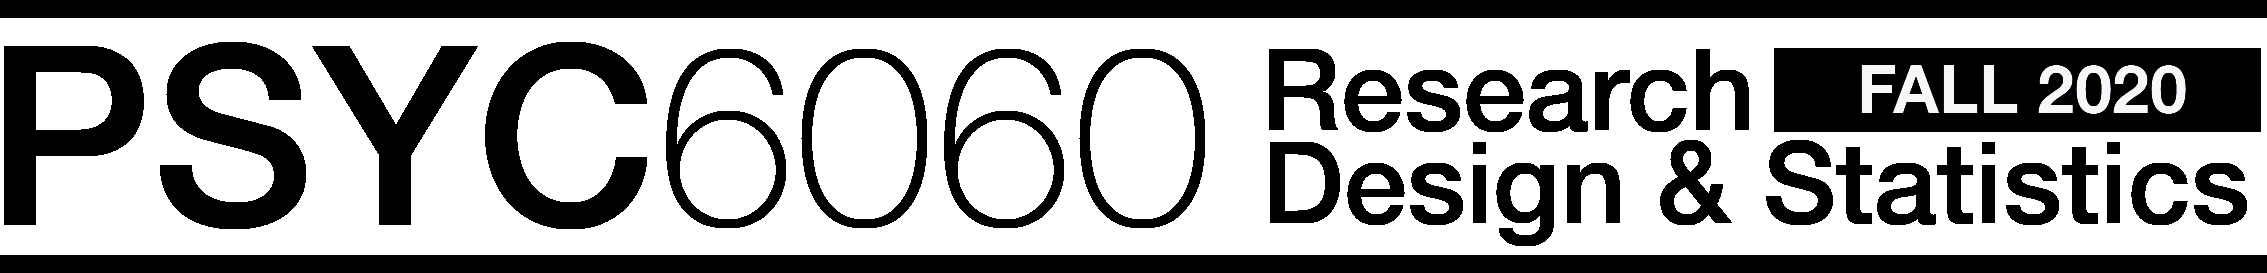
\includegraphics[width=1\linewidth]{header_6060}

These notes are a resource for students in my PSYC 6060 class. The notes are a subset of material that I am creating for a public domain statistics book to be released sometime in the distant future.

\chapter*{About the Author}\label{about-the-author}


David J. Stanley is an Associate Professor of Industrial \& Organizational Psychology in Canada. He obtained a BA in \href{https://uwaterloo.ca/psychology/}{Psychology}, with a Minor in \href{https://uwaterloo.ca/math/}{Statistics}, from University of Waterloo and his PhD in \href{https://psychology.uwo.ca}{Psychology} from Western University in London, Ontario. David has published articles in Advances in Methods and Practices in Psychological Science, Organizational Research Methods, Journal of Applied Psychology, Perspectives in Psychological Science, Journal of Business and Psychology, Journal of Vocational Behaviour, Journal of Personality and Social Psychology, Behavior Research Methods, Industrial and Organizational Psychology, and Emotion among other journals. David also created the \href{https://CRAN.R-project.org/package=apaTables}{apaTables} \emph{R} package that has more than 350,000 downloads.

\mainmatter

\chapter{Introduction}\label{introduction}

Welcome! In this guide, we will teach you about statistics using the statistical software R with the interface provided by R Studio. The purpose of this chapter to is provide you with a set of activities that get you up-and-running in R quickly so get a sense of how it works. In later chapters we will revisit these same topics in more detail.

\section{A focus on workflow}\label{a-focus-on-workflow}

An important part of this guide is training you in a workflow that will avoid many problems than can occur when using R.

\section{R works with plug-ins}\label{r-works-with-plug-ins}

R is a statistical language with many plug-ins called \textbf{packages} that you will use for analyses. You can think of R as being like your smartphone. To do things with your phone you need \textbf{an App} (R equivalent: a \emph{package}) from the App Store (R equivalent: \emph{CRAN}). Apps need to be \textbf{downloaded} (R equivalent: \emph{install.packages}) before you can use them. To use the app you need \textbf{Open} it (R equivalent: \emph{library command}). These similarities are illustrated in Table \ref{tab:appstore} below.

\begin{table}

\caption{\label{tab:appstore}R packages are similar to smart phone apps (Kim, 2018)}
\centering
\begin{tabular}[t]{ll}
\toprule
Smart Phone Terminology & R Terminology\\
\midrule
App & package\\
App Store & CRAN\\
Download App from App Store & install.packages("apaTables" , dependencies = TRUE)\\
Open App & library("apaTables")\\
\bottomrule
\end{tabular}
\end{table}

\section{Software Choice}\label{software-choice}

The software for this course is free and runs on Mac or PC/Windows. If you do not have a Mac or PC but instead are working with a tablet - contact the instructor during office hours.

\subsection{Mac}\label{mac}

On a Mac you need to download and install R and RStudio. The RStudio software is a ``front end'' for using R. Although you need to download and install both - you will only ever load RStudio.

\subsubsection{Mac Download R}\label{mac-download-r}

\begin{itemize}
\item
  Go to this \href{https://cloud.r-project.org}{link} to download the latest version of R. On the screen that appears select ``Download R for (Mac) OS X''.
\item
  On the next screen you will see something like the image below. However, the number (4.0.3) will be different you. Download this file.
\end{itemize}

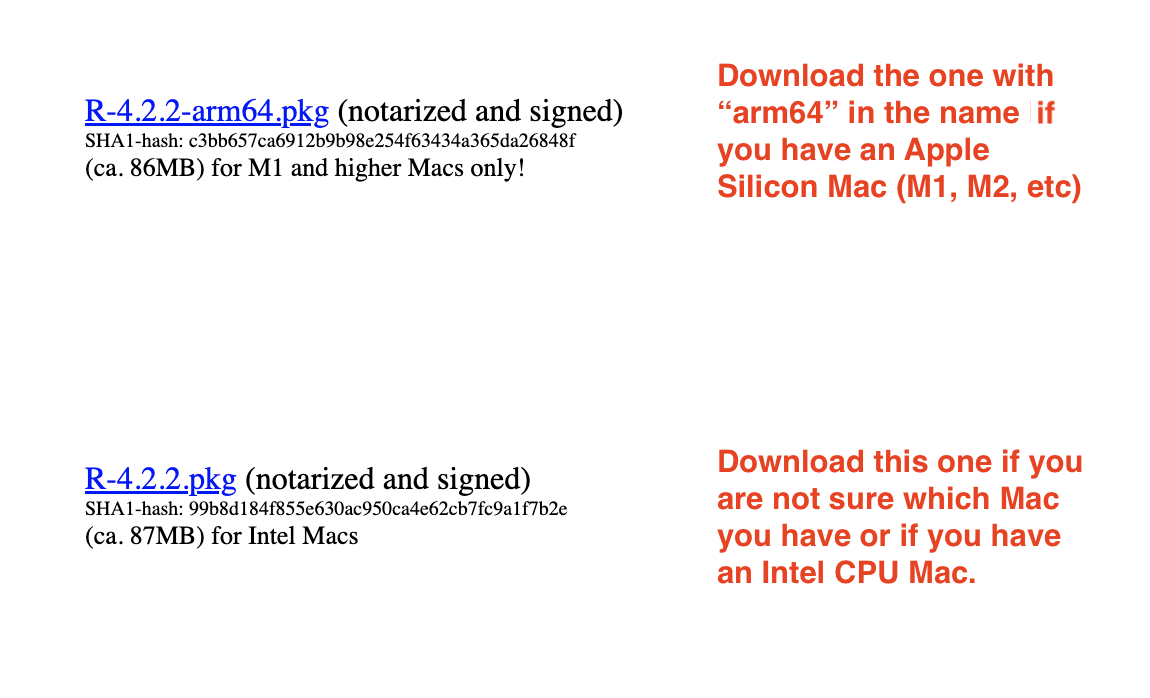
\includegraphics[width=0.75\linewidth]{ch_introduction/images/screenshot_mac_r}

\begin{itemize}
\item
  Run the file you just downloaded to install R.
\item
  Remember you will never run R - you just need it installed so you can use RStudio.
\item
  Now install RStudio (see below)
\end{itemize}

\subsubsection{Mac Download RStudio}\label{mac-download-rstudio}

After installing R you will install RStudio. This is the software you will actually use in this course.

\begin{itemize}
\tightlist
\item
  Go to this \href{https://posit.co/download/rstudio-desktop/}{link} to download the latest version of RStudio. On the page that appears scroll down until you see the following:
\end{itemize}

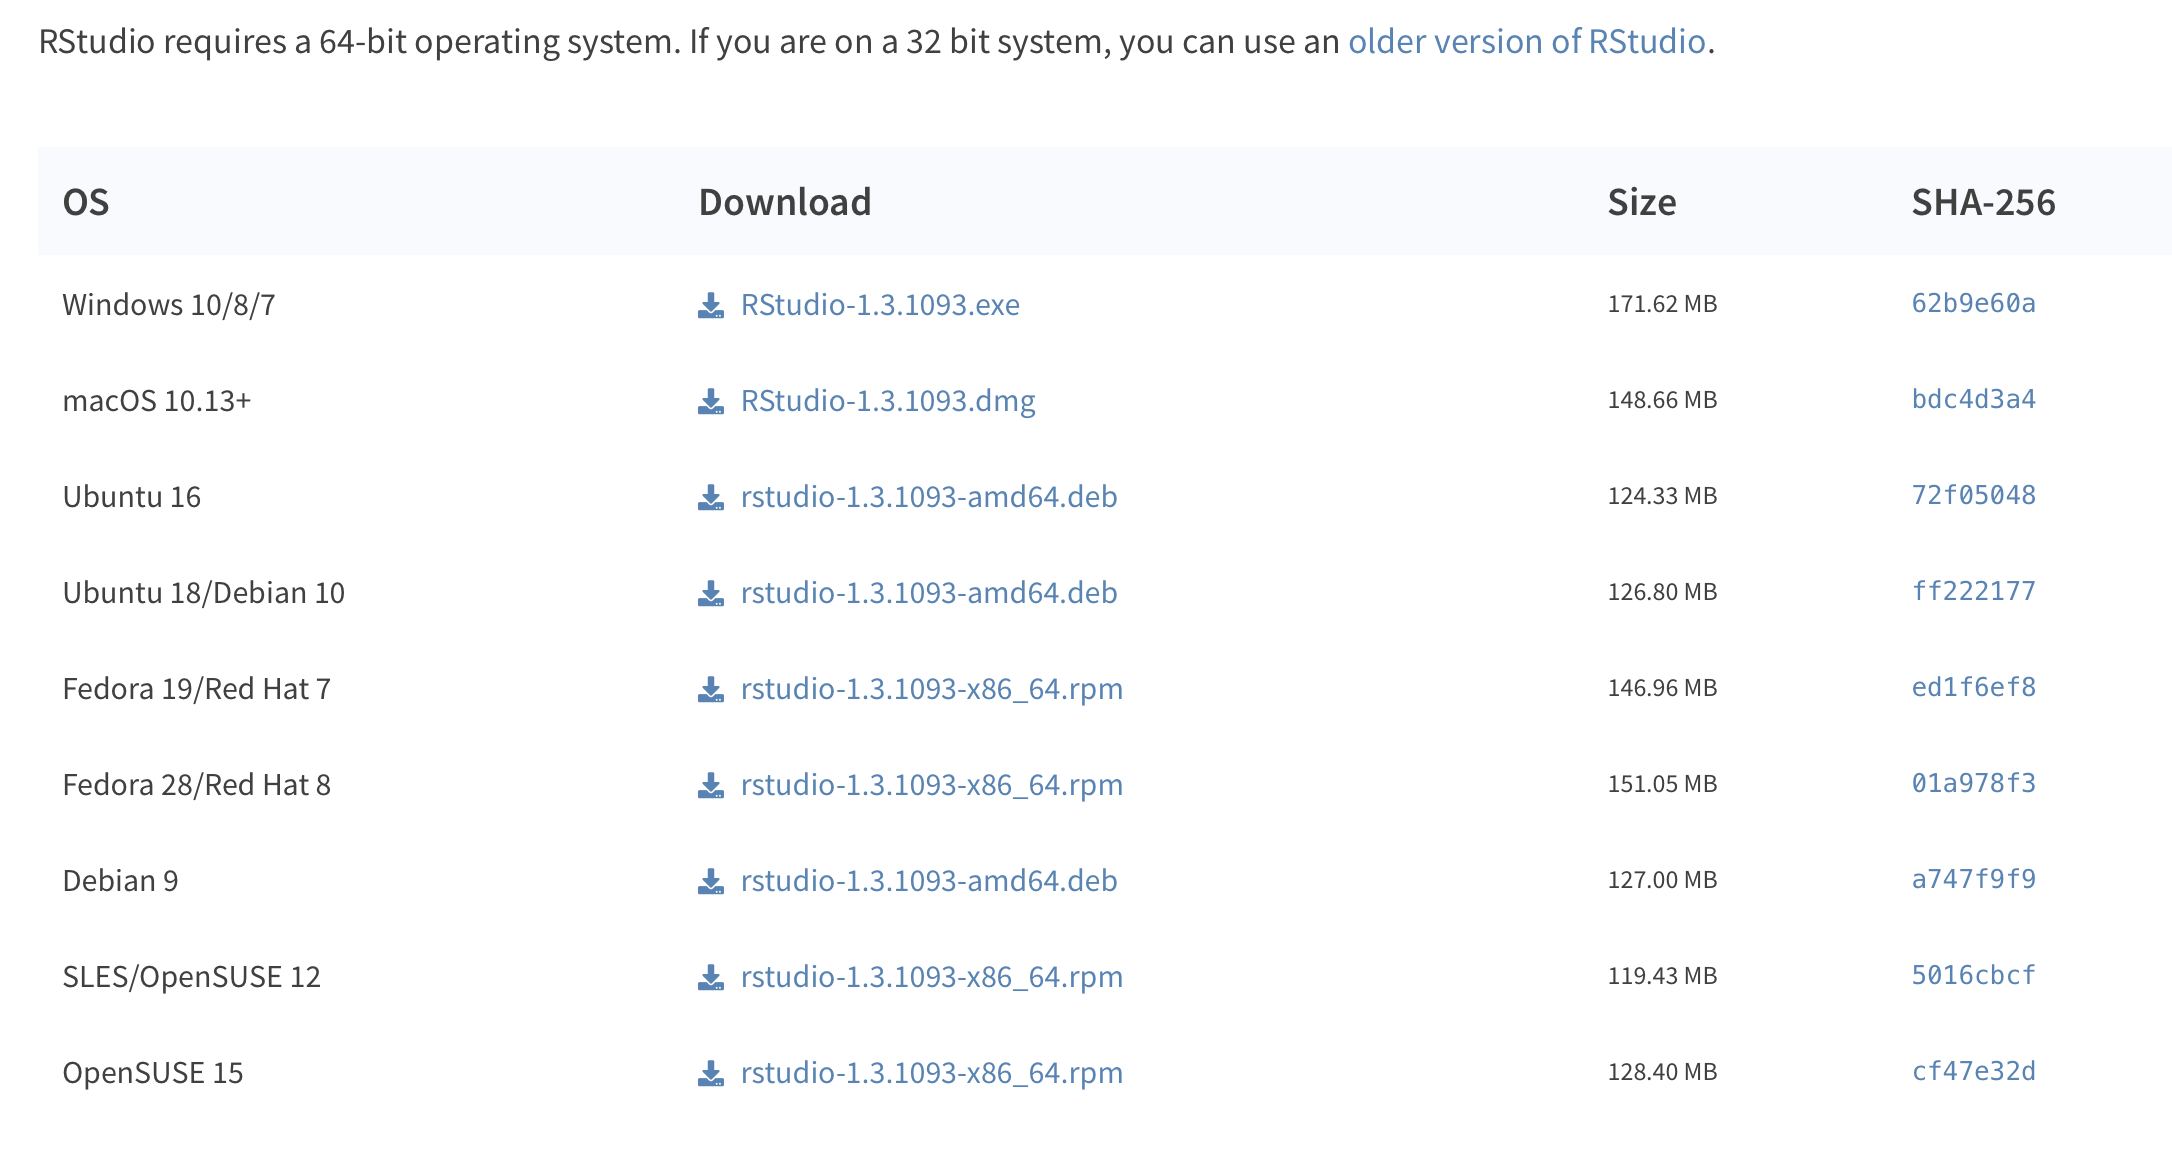
\includegraphics[width=0.75\linewidth]{ch_introduction/images/screenshot_rstudio}

\begin{itemize}
\item
  Look at the line for Mac users and download the file. Here it is: RStudio-1.3.1093.dmg your numbers will be different - but this is the file you need. Download it.
\item
  Open the file you downloaded. You should see something like the screenshot below. Drag the RStudio icon to the Applications folder to install it.
\end{itemize}

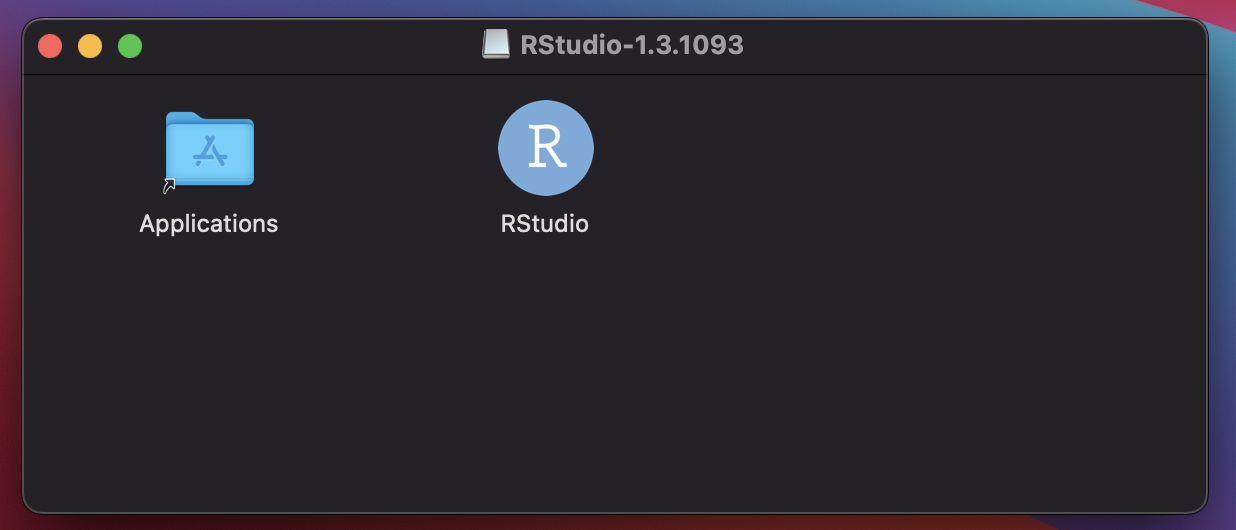
\includegraphics[width=0.75\linewidth]{ch_introduction/images/screenshot_dmg}

\begin{itemize}
\tightlist
\item
  In the future, when you want to run RStudio you should do so from the Applications folder. You can access the Applications folder using the Menu shown below. This will open the applications folder.
\end{itemize}

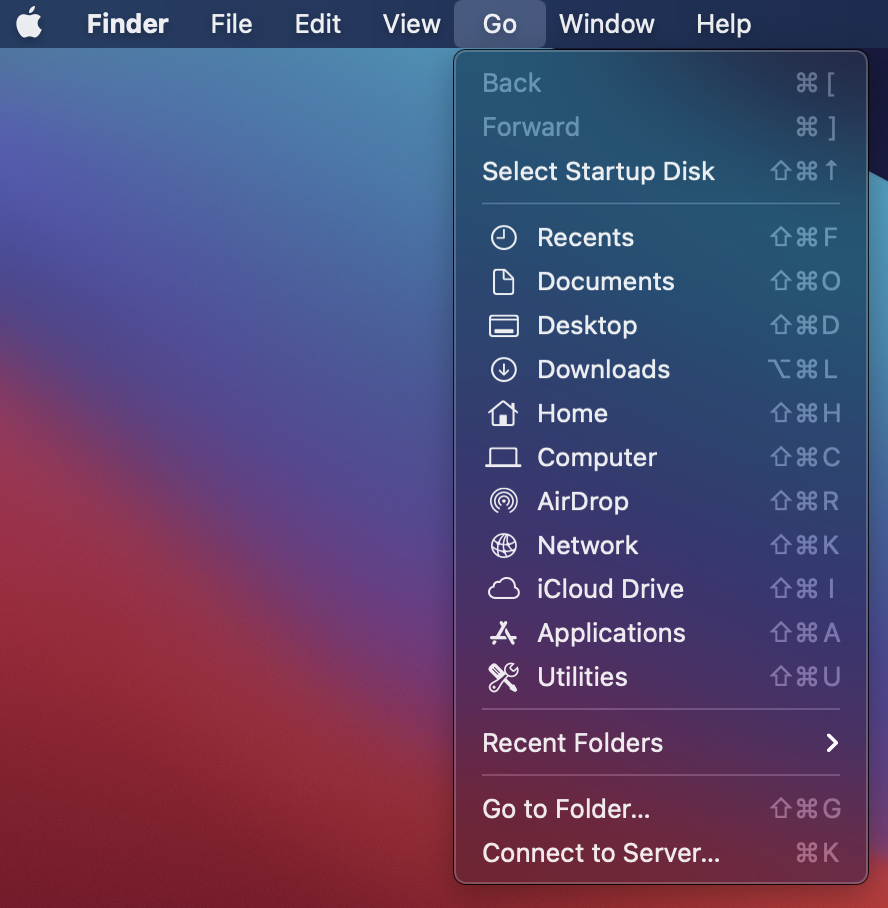
\includegraphics[width=0.35\linewidth]{ch_introduction/images/screenshot_applications}

\begin{itemize}
\tightlist
\item
  In the Applications folder there is now an RStudio icon. Click this icon to run RStudio each time you use it. You can also drag the RStudio icon in the Applications folder to the Dock for easy access if you prefer.
\end{itemize}

\subsection{PC}\label{pc}

\subsubsection{PC Download R}\label{pc-download-r}

\begin{itemize}
\item
  Go to this \href{https://cloud.r-project.org}{link} to download the latest version of R. On the screen that appears select ``Download R for Windows''.
\item
  On the next screen you will see something like the image below. Select ``base''.
\end{itemize}

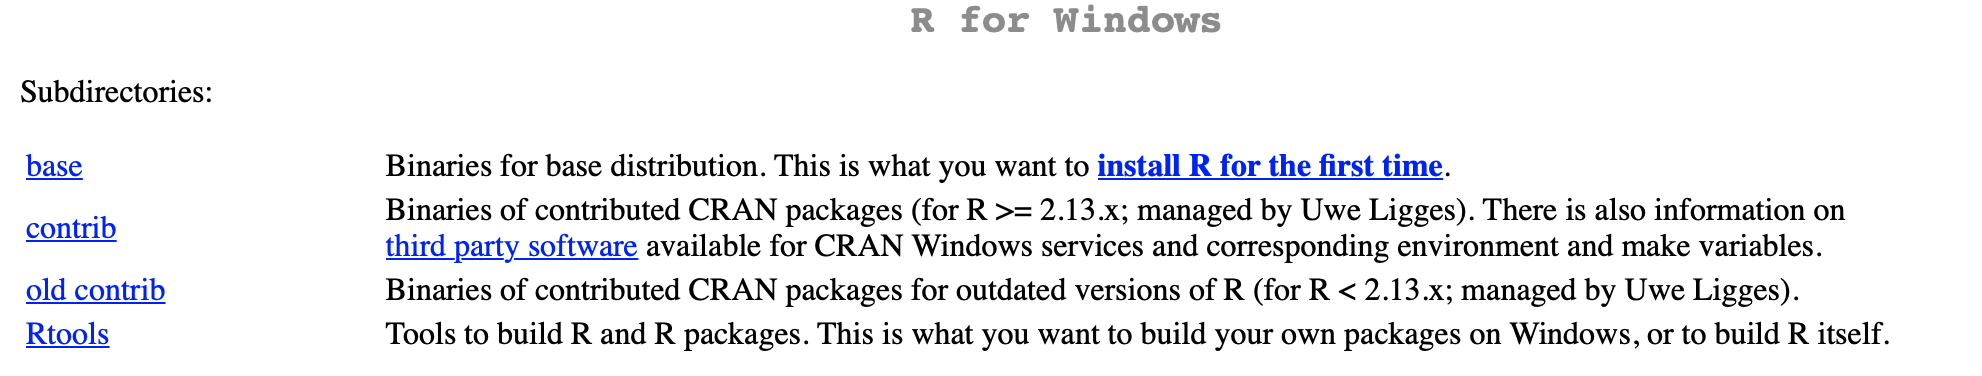
\includegraphics[width=0.75\linewidth]{ch_introduction/images/screenshot_pc_r}

\begin{itemize}
\tightlist
\item
  On the next screen you will see something like the image below. As before the specific file numbers will differ for you. Select ``Download R 4.0.3 for Windows'' and download it.
\end{itemize}

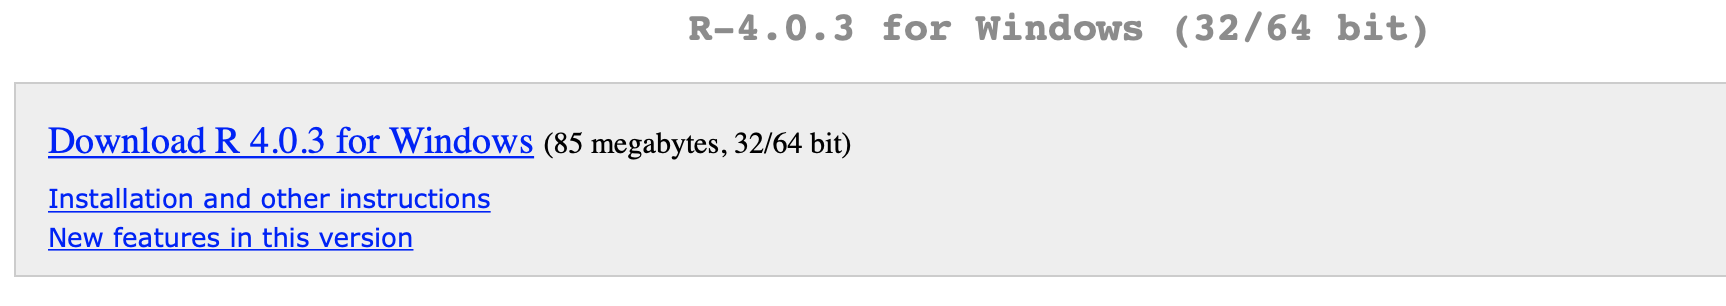
\includegraphics[width=0.75\linewidth]{ch_introduction/images/screenshot_pc_base}

\begin{itemize}
\item
  Run the file you just downloaded to install R.
\item
  Remember you will never run R - you just need it installed so you can use RStudio.
\item
  Now install RStudio
\end{itemize}

\subsubsection{PC Download RStudio}\label{pc-download-rstudio}

After installing R you will install RStudio. This is the software you will actually use in this course.

\begin{itemize}
\tightlist
\item
  Go to this \href{https://posit.co/download/rstudio-desktop/}{link} to download the latest version of RStudio. On the page that appears scroll down until you see the following:
\end{itemize}

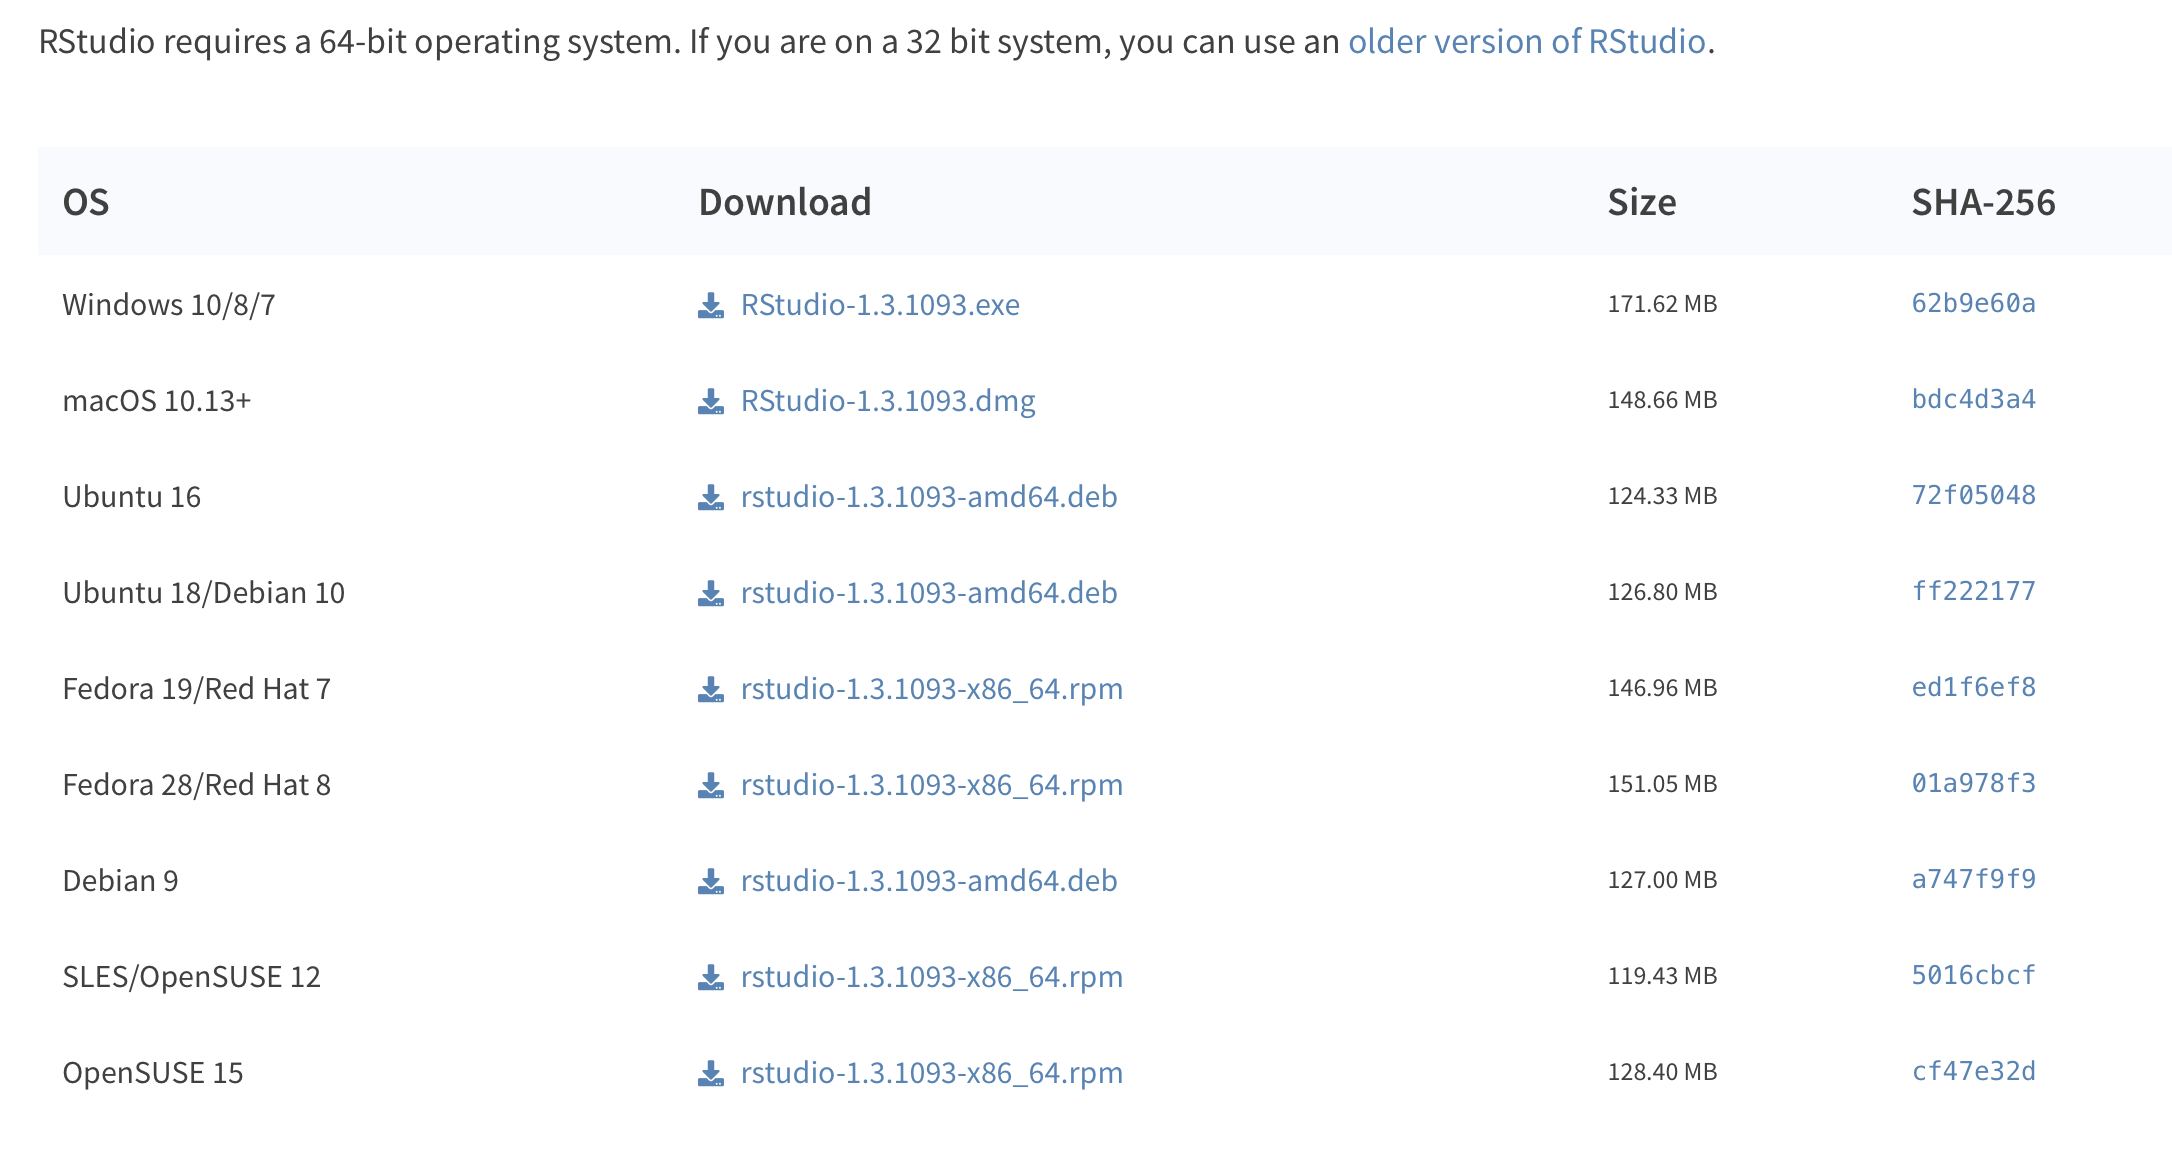
\includegraphics[width=0.75\linewidth]{ch_introduction/images/screenshot_rstudio}

\begin{itemize}
\item
  Look at the line for ``Windows 10/8/7'' users and download the file. Here it is: RStudio-1.3.1093.exe your numbers will be different - but this is the file you need. Download it.
\item
  Open the file you downloaded and run it to install RStudio.
\item
  In the future you will only use RStudio to access use R.
\end{itemize}

\section{Run RStudio not R}\label{run-rstudio-not-r}

As noted above, in the future you will run RStudio to use R. That is, you click the icon below to use RStudio moving forward. On macOs make sure it is the icon in the Applications folder. On Windows make sure it is the icon in the Program Files folder.


\includegraphics[width=0.3\linewidth]{ch_introduction/images/rstudio_icon}

\section{RStudio configuration, First run only}\label{rstudio-configuration-first-run-only}

Prior using RStudio it is important it to configure it properly to avoid problems getting your code to work. Therefore, the very first time you run RStudio you should configure it correctly.

As illustrated below, go to the Tools menu and select Global Options\ldots{}

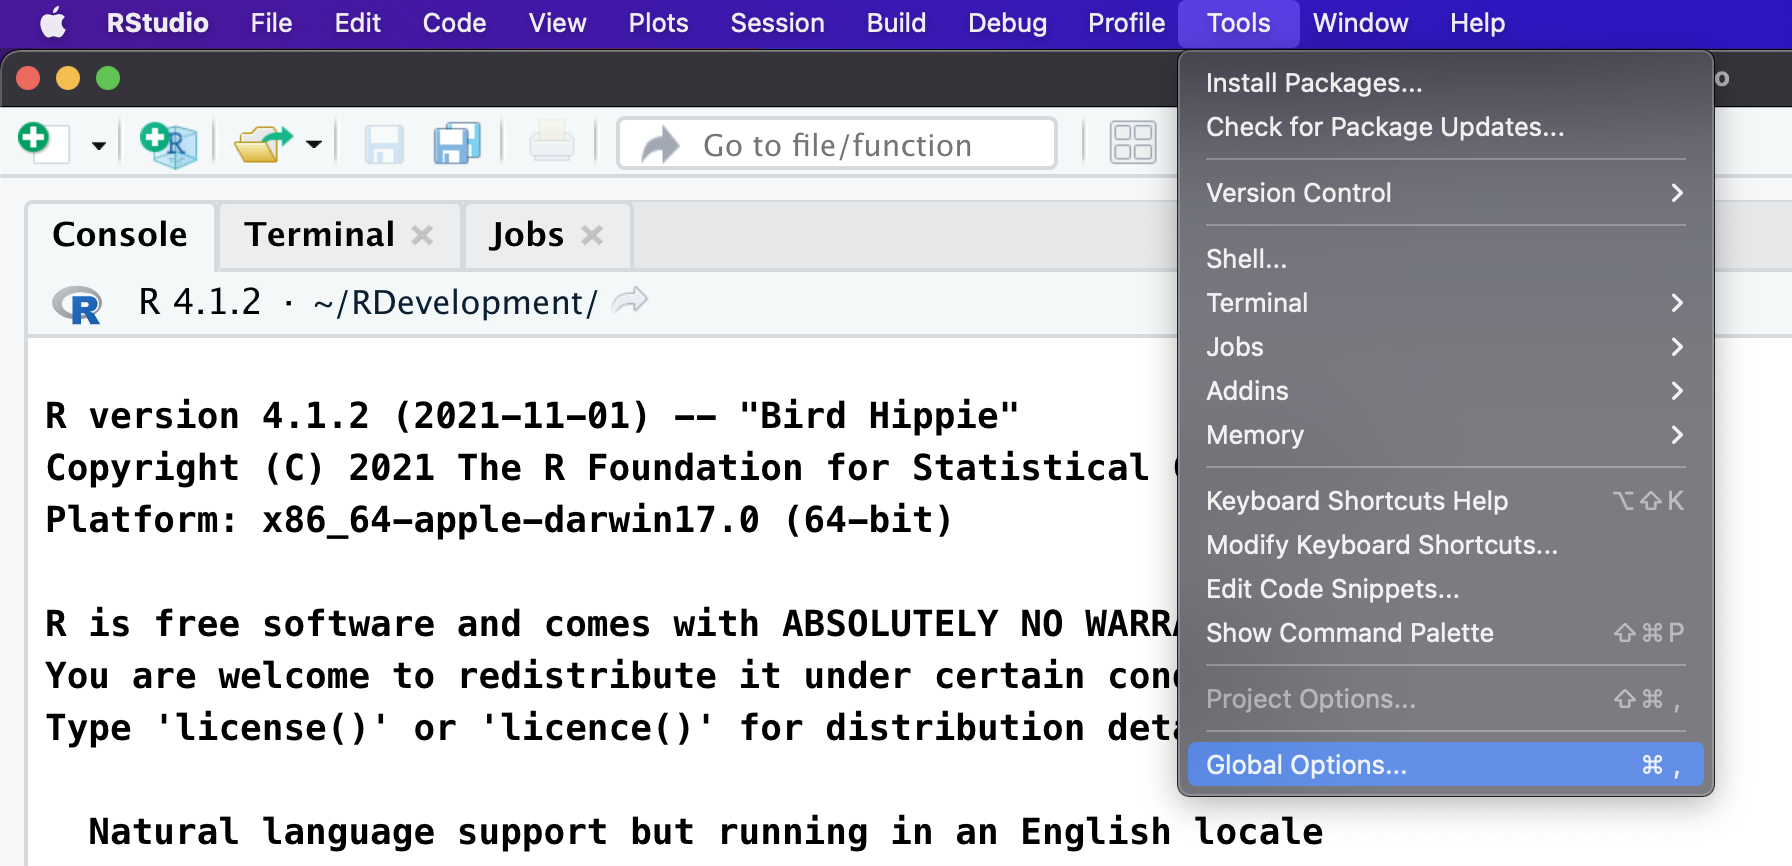
\includegraphics[width=0.7\linewidth]{ch_introduction/images/screenshot_global_menu}

Next, ensure General is selected on the left side. Then ensure that ``Restore .RData into workspace at startup'' is not checked. I repeat, NOT CHECKED. Also, make sure that ``Save workspace to .RData on exit'' is set to NEVER. Then click the OK button at the bottom of the window.

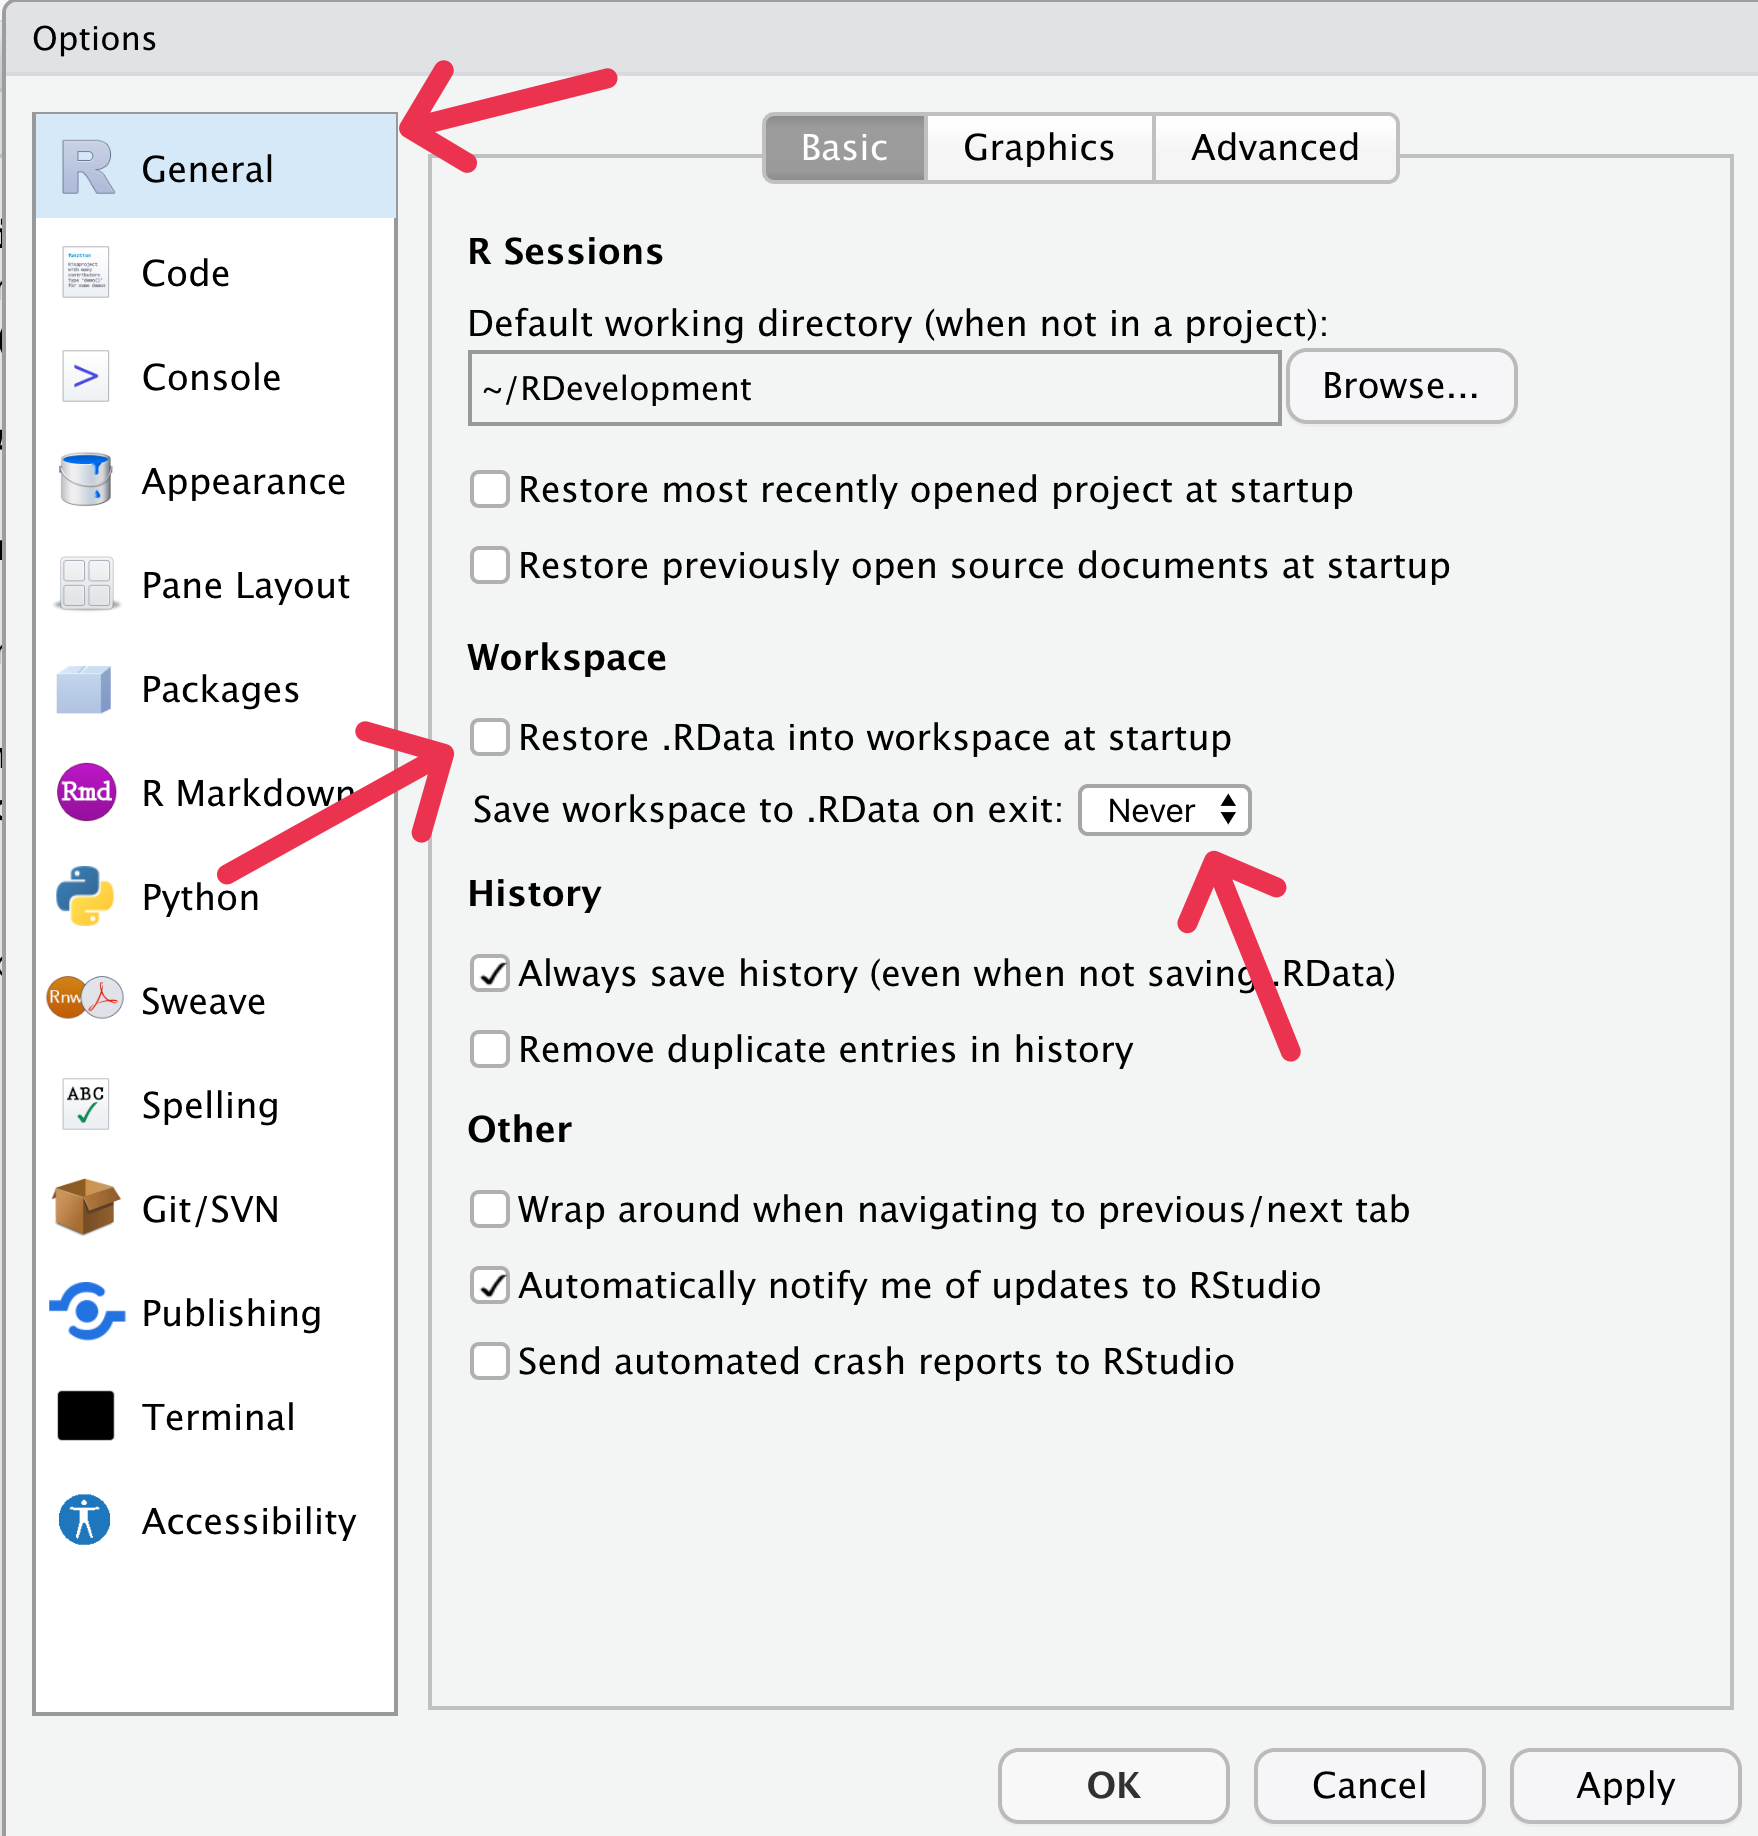
\includegraphics[width=0.7\linewidth]{ch_introduction/images/screenshot_global_details}

\section{Begin with an RStudio Project}\label{begin-with-an-rstudio-project}

It can be hard to keep track of files you use and create when using RStudio. Therefore, you should always use an RStudio Project to keep track of things. This is basically just a Folder on your computer that RStudio associates with a particular task. Later in this introduction to RStudio we will use the file data\_okcupid.csv. Right now we will set up a Project to make it easier to use that file.

\begin{enumerate}
\def\labelenumi{\arabic{enumi}.}
\item
  Create a folder on your computer called ``psyc6060\_project\_1''. Be sure you know where you create this folder so you can find it again easily.
\item
  Download the \url{data_okcupid.csv} file. \textbf{NOTE:You must get this file from your Downloads folder. For many people (on macOS) the file may Open in Numbers - then they are tempted to save it from Numbers. This will not work. Just close Numbers. Then retrieve the file from you Downloads folder.}
\item
  Place the data\_okcupid.csv file into the psyc6060\_project\_1 folder.
\item
  Load RStudio.
\item
  Go to the File menu and select ``New Project\ldots{}''
\item
  You will see the window below. Select ``Existing Directory''.
\end{enumerate}

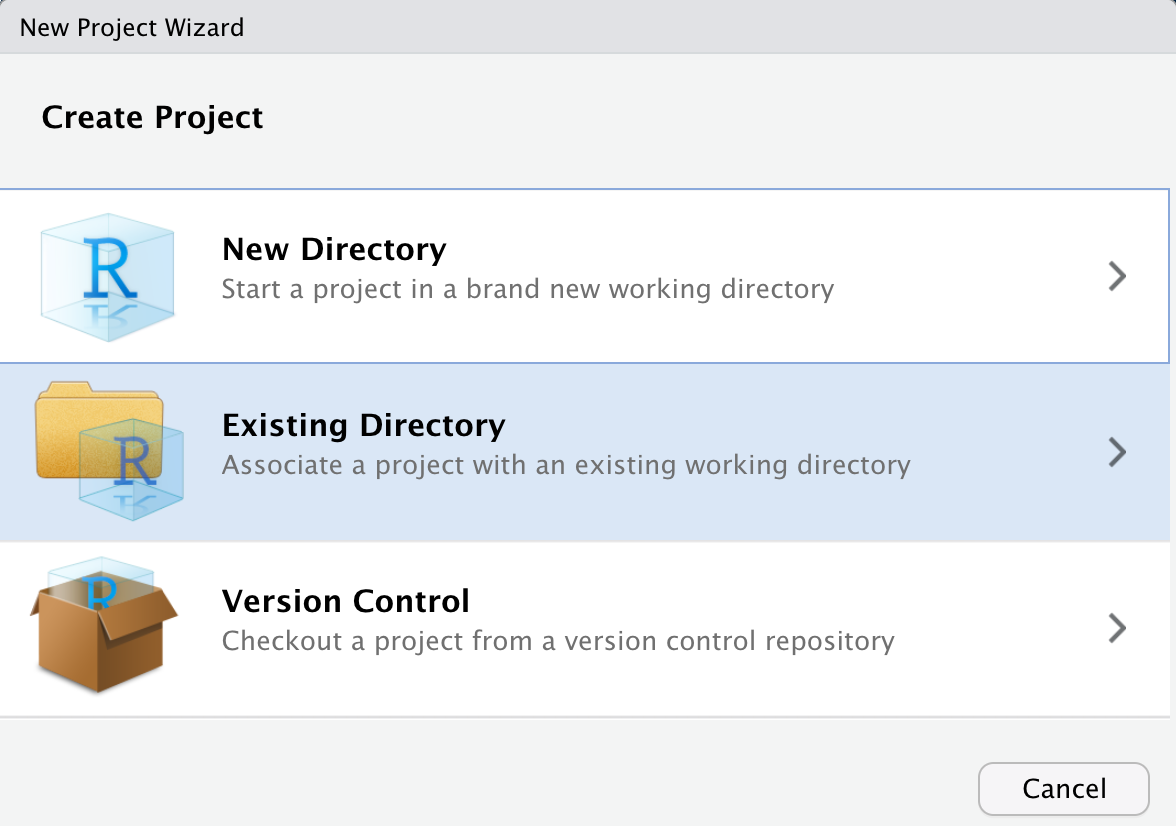
\includegraphics[width=0.5\linewidth]{ch_introduction/images/screenshot_new_project}

\begin{enumerate}
\def\labelenumi{\arabic{enumi}.}
\setcounter{enumi}{6}
\tightlist
\item
  You will see the window below. Click the ``Browse'' button and then locate the folder you created. Once this is done click the ``Create Project'' button.
\end{enumerate}

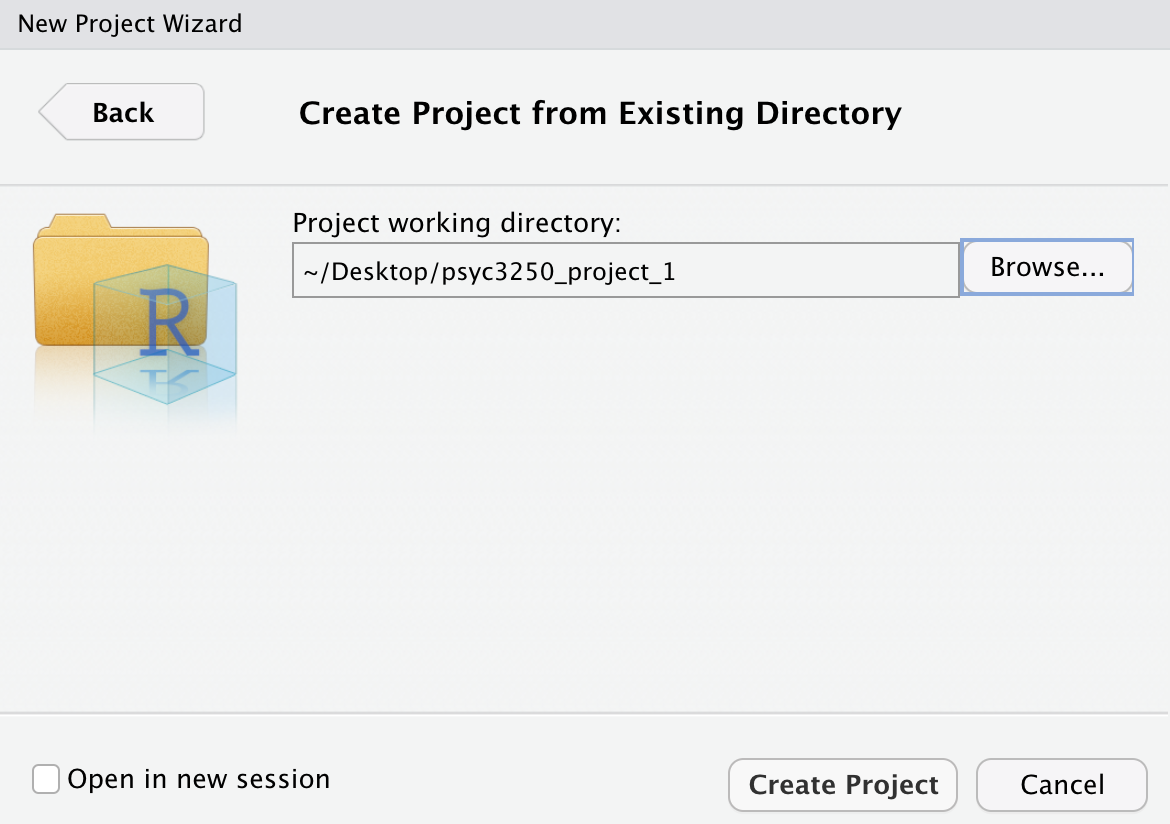
\includegraphics[width=0.5\linewidth]{ch_introduction/images/screenshot_create_project}

\begin{enumerate}
\def\labelenumi{\arabic{enumi}.}
\setcounter{enumi}{7}
\tightlist
\item
  You're ready to begin. Follow this process of creating an RStudio project for each class project/activity.
\end{enumerate}

\section{Exploring the R Studio Interface}\label{exploring-the-r-studio-interface}

Once you have opened (or created) a Project folder, you are presented with the R Studio interface. There are a few key elements to the user interface that are illustrated in Figure \ref{fig:interface} In the lower right of the screen you can see the a panel with several tabs (i.e., Files, Plots, Packages, etc) that I will refer to as the Files pane. You look in this pane to see all the files associated with your project. On the left side of the screen is the Console which is an interactive pane where you type and obtain results in real time. I've placed two large grey blocks on the screen with text to more clearly identify the Console and Files panes. Not shown in this figure is the Script panel where we can store our commands for later reuse.

\begin{figure}
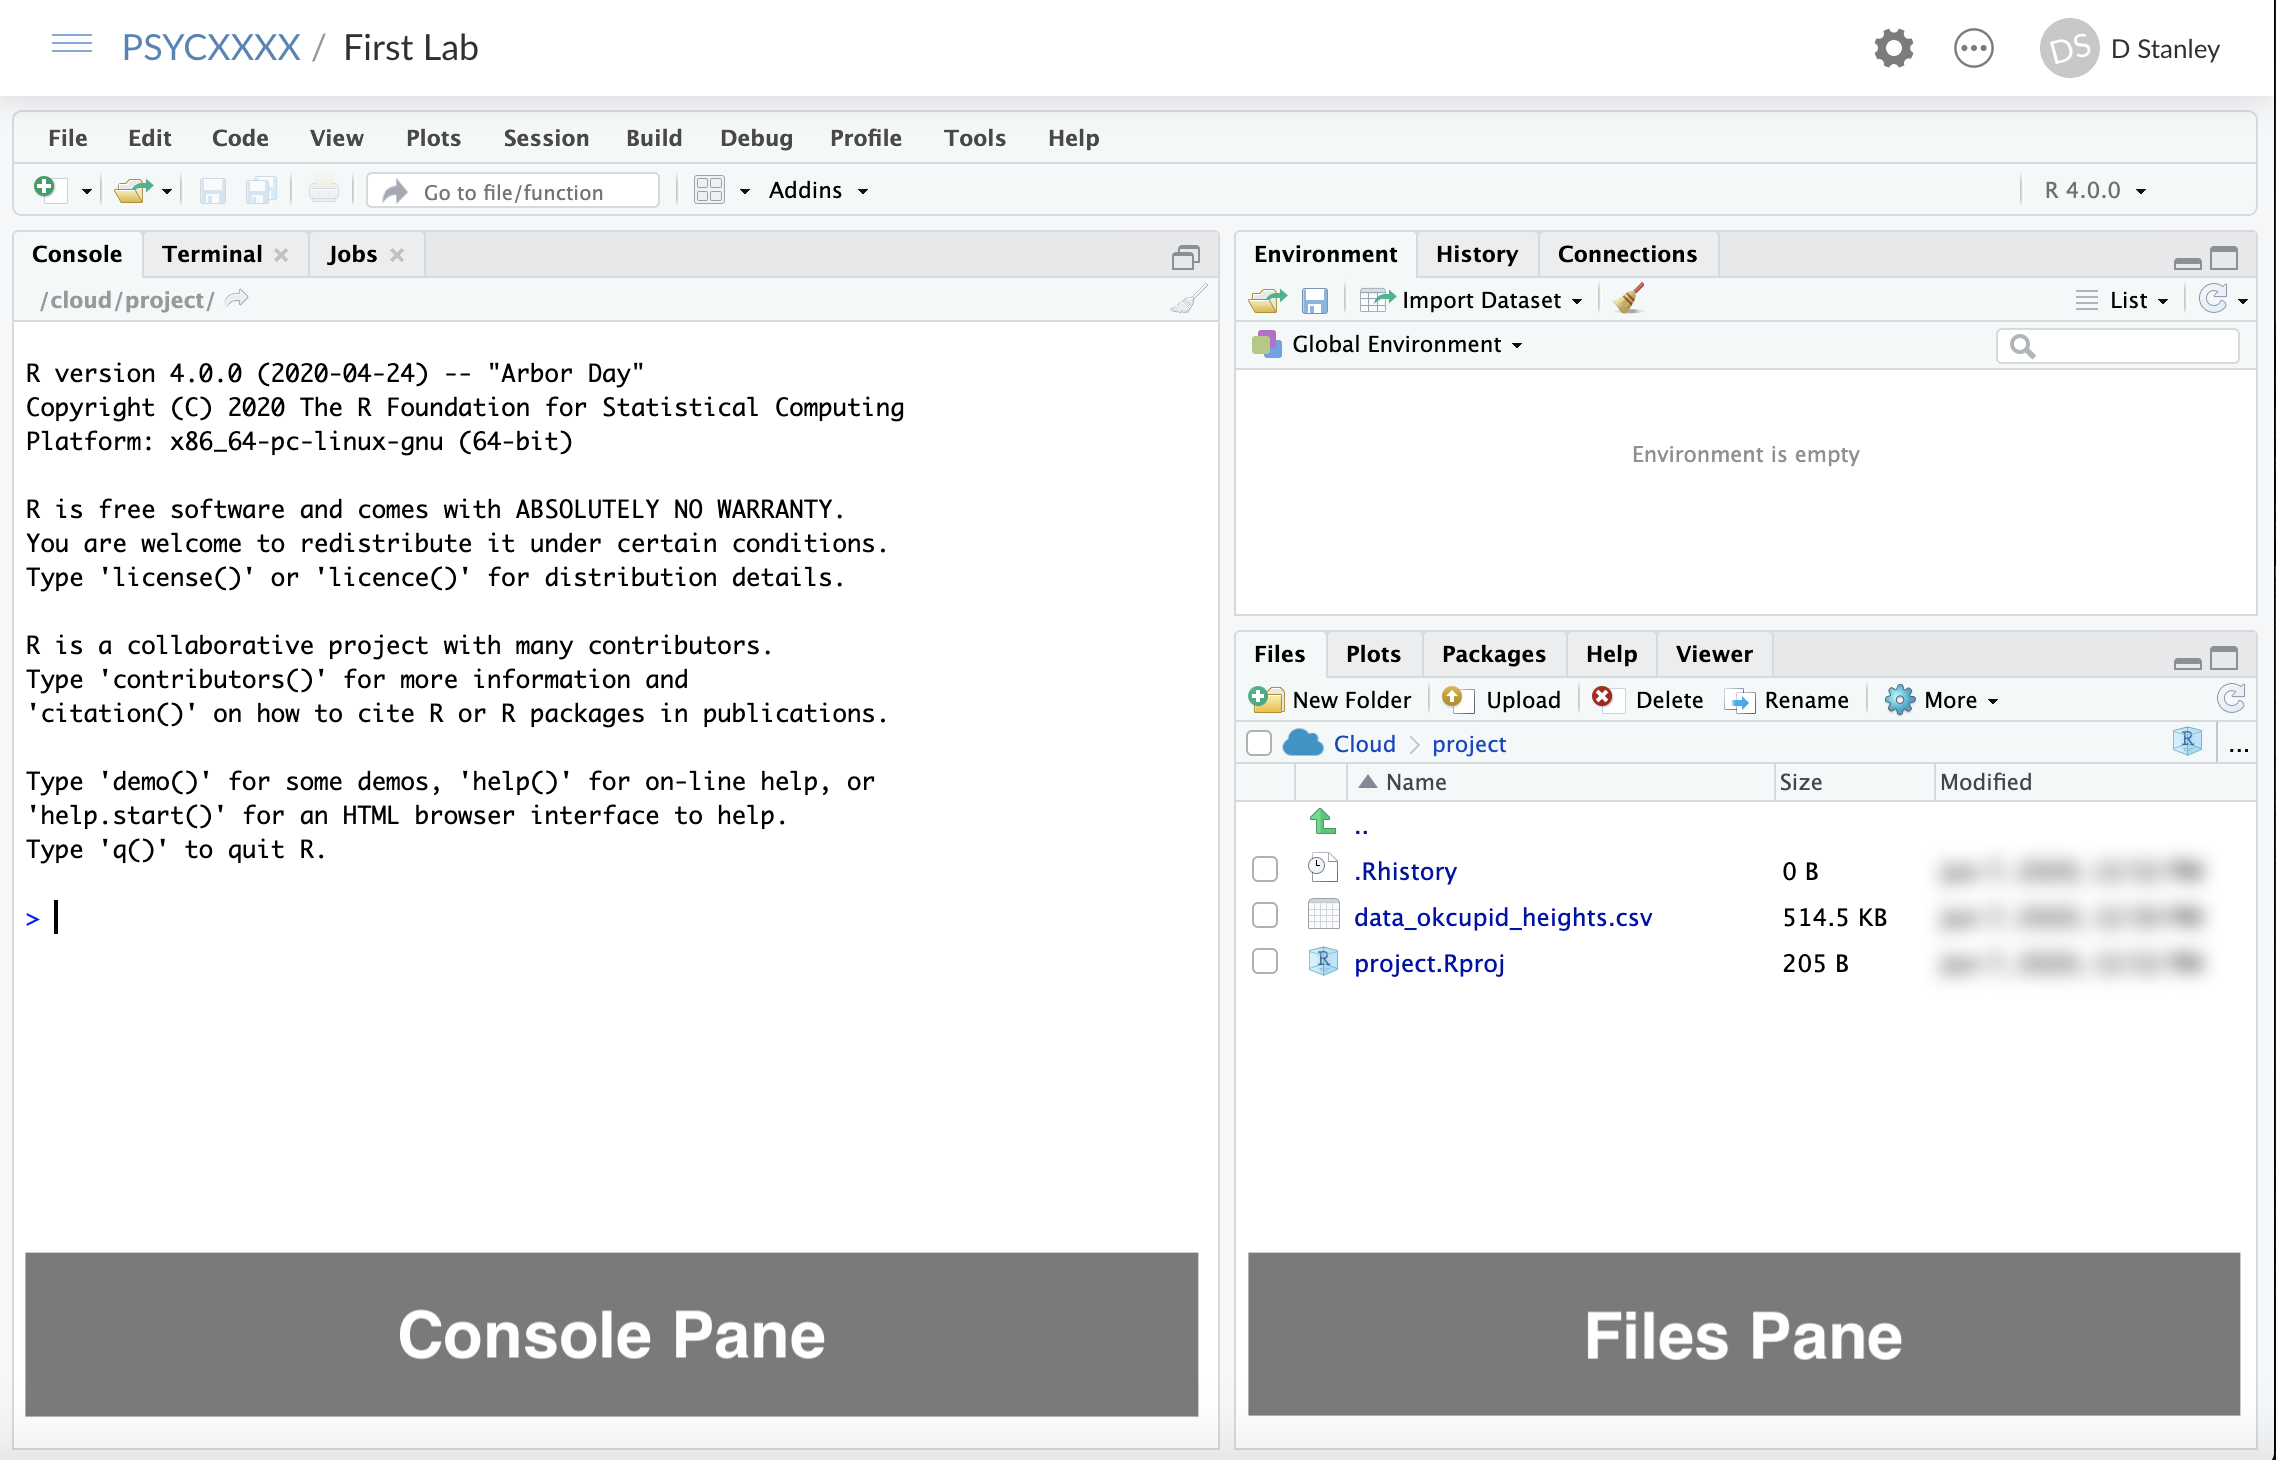
\includegraphics[width=0.7\linewidth]{ch_introduction/images/screenshot_interface} \caption{R Studio interface}\label{fig:interface}
\end{figure}

\subsection{Console panel}\label{console-panel}

When you first start R, the Console panel is on the left side of the screen. Sometimes there are two panels on the left side (one above the other); if so, the Console panel is the lower one (and labeled accordingly). We can use R a bit like a calculator. Try typing the following into the Console window: 8 + 6 + 7 + 5. You can see that R immediately produced the result on a line preceded by two hashtags (\#\#).

\begin{Shaded}
\begin{Highlighting}[]
\DecValTok{8} \SpecialCharTok{+} \DecValTok{6} \SpecialCharTok{+} \DecValTok{7} \SpecialCharTok{+} \DecValTok{5}
\end{Highlighting}
\end{Shaded}

\begin{verbatim}
## [1] 26
\end{verbatim}

We can also put the result into a variable to store it. Later we can use the print command to see that result. In the example below we add the numbers 3, 0, and 9 and store the result in the variable my\_sum. The text ``\textless-'' indicate you are putting what is on the right side of the arrow into the variable on the left side of the arrow. You can think of a variable as cup into which you can put different things. In this case, imagine a real-world cup with my\_sum written on the outside and inside the cup we have stored the sum of 3, 0, and 9 (i.e., 12).

\begin{Shaded}
\begin{Highlighting}[]
\NormalTok{my\_sum }\OtherTok{\textless{}{-}} \DecValTok{3} \SpecialCharTok{+} \DecValTok{0} \SpecialCharTok{+} \DecValTok{9}
\end{Highlighting}
\end{Shaded}

We can inspect the contents of the my\_sum variable (i.e., my\_sum cup) with the print command:

\begin{Shaded}
\begin{Highlighting}[]
\FunctionTok{print}\NormalTok{(my\_sum)}
\end{Highlighting}
\end{Shaded}

\begin{verbatim}
## [1] 12
\end{verbatim}

Variable are very useful in R. We will use them to store a single number, an entire data set,
the results of an analysis, or anything else.

\subsection{Script Panel}\label{script-panel}

Although you can use R with just with the Console panel, it's a better idea to use scripts via the Script panel - not visible yet. Scripts are just text files with the commands you use stored in them. You can run a script (as you will see below) using the Run or Source buttons located in the top right of the Script panel.

Scripts are valuable because if you need to run an analysis a second time you don't have to type the command in a second time. You can run the script again and again without retyping your commands. More importantly though, the script provides a record of your analyses.

A common problem in science is that after an article is published, the authors can't reproduce the numbers in the paper. You can read more about the important problem in a surprising article in the journal \href{https://molecularbrain.biomedcentral.com/articles/10.1186/s13041-020-0552-2}{Molecular Brain}. In this article an editor reports how a request for the data underlying articles resulted in the wrong data for 40 out of 41 papers. Long story short -- keep track of the data and scripts you use for your paper. In a later chapter, it's generally poor practice to manipulate or modify or analyze your data using any menu driven software because this approach does not provide a record of what you have done.

\section{Writing your first script}\label{writing-your-first-script}

\subsection{Create the script file}\label{create-the-script-file}

Create a script in your R Studio project by using the menu File \textgreater{} New File \textgreater{} R Script.

Save the file with an appropriate name using the File menu. The file will be saved in your Project folder. A common, and good, convention for naming is to start all script names with the word ``script'' and separate words with an underscore. You might save this first script file with the name ``script\_my\_first\_one.R''. The advantage of beginning all script files with the word script is that when you look at your list of files alphabetically, all the script files will cluster together. Likewise, it's a good idea to save all data files such that they begin with ``data\_''. This way all the data files will cluster together in your directory view as well. You can see there is already a data file with this convention called ``data\_okcupid.csv''.

You can see as discussed previously, we are trying to instill an effective workflow as you learn R. Using a good naming convention (that is consistent with what others use) is part of the workflow. When you write your scripts it's a good idea to follow the \href{https://style.tidyverse.org}{tidyverse style guide} for script names, variable name, file names, and more.

\subsection{Add a comment to your script}\label{add-a-comment-to-your-script}

In the previous section you created your first script. We begin by adding a comment to the script. A comment is something that will be read by humans rather than the computer/R. You make comments for other people that will read your code and need to understand what you have done. However, realize that you are also making comments for your future self as illustrated in an \href{https://xkcd.com/1421/}{XKCD cartoon}.

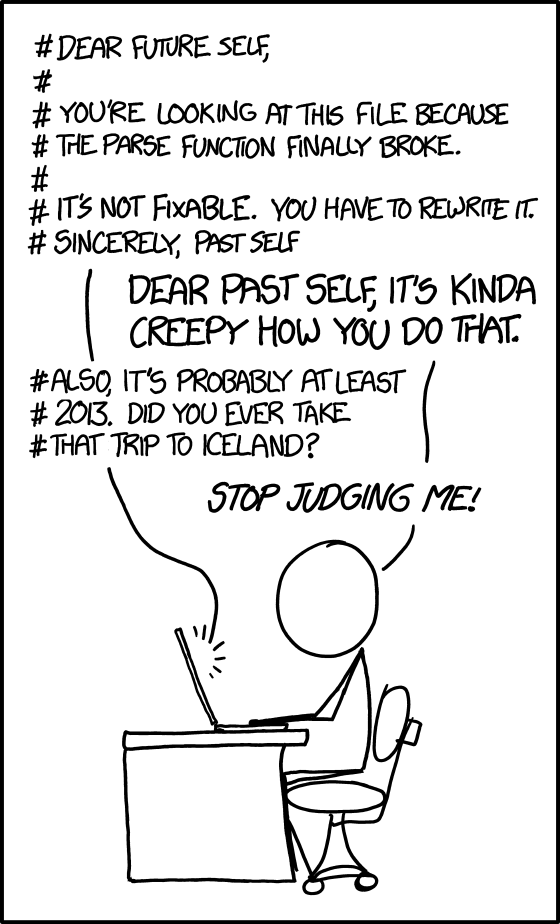
\includegraphics[width=0.4\linewidth]{ch_introduction/images/future_self_2x}

A good way to start every script is with a comment that includes the date of your script (or even better when you installed your packages, more on this later). Like smartphone apps, packages are updated regularly. Sometimes after a package is updated it will no longer work with an older script. Fortunately, the \href{https://cran.r-project.org/web/packages/checkpoint/index.html}{checkpoint package}\index{R Studio Cloud} lets users role back the clock and use older versions of packages. Adding a comment with the date of your script will help future users (including you) to use your script with the same version of the package used when you wrote the script. Dating your script is an important part of an effective and reproducible workflow.

\begin{Shaded}
\begin{Highlighting}[]
\CommentTok{\# Code written on: YYYY/MM/DD }
\CommentTok{\# By: John Smith}
\end{Highlighting}
\end{Shaded}

Moving forward, I suggest you use comments to make your own personal notes in your own code as your write it. Note that in the above comment I used the internationally accepted date format\index{date format} order Year/Month/Day created by the \href{https://www.iso.org/home.html}{International Organization for Standardization} (ISO). Some people use the mnemonic \emph{You're My Dream} to remember the \textbf{Y}ear \textbf{M}onth \textbf{D}ay order. Wikipedia provides more information about this \href{https://en.wikipedia.org/wiki/ISO_8601}{International Date Format (ISO 8601)}. An \href{https://xkcd.com/1179/}{XKCD} cartoon highlights the ISO date format:

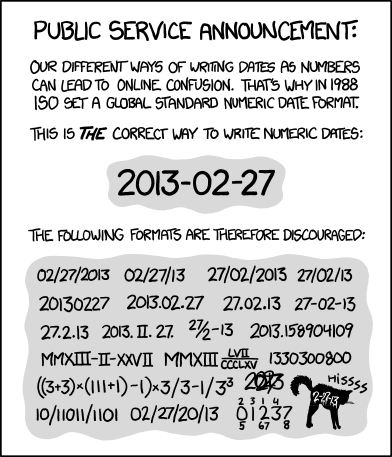
\includegraphics[width=0.4\linewidth]{ch_introduction/images/iso8601}

\subsection{Background about the tidyverse}\label{background-about-the-tidyverse}

There are generally two broad ways of using R, the older way and the newer way. Using R the older way is referred to as using base R. A more modern approach to using R is the tidyverse\index{tidyverse}. The tidyverse represents a collection of packages the work together to give R a modern workflow. These packages do many things to help the data analyst (loading data, rearranging data, graphing, etc.). We will use the tidyverse approach to R in this guide.

A noted the tidyverse is a collection of packages. Each package adds new commands to R. The number of packages and correspondingly the number of new commands added to R by the tidyverse is large. Below is a list of the tidyverse packages:

\begin{verbatim}
##  [1] "broom"         "conflicted"    "cli"          
##  [4] "dbplyr"        "dplyr"         "dtplyr"       
##  [7] "forcats"       "ggplot2"       "googledrive"  
## [10] "googlesheets4" "haven"         "hms"          
## [13] "httr"          "jsonlite"      "lubridate"    
## [16] "magrittr"      "modelr"        "pillar"       
## [19] "purrr"         "ragg"          "readr"        
## [22] "readxl"        "reprex"        "rlang"        
## [25] "rstudioapi"    "rvest"         "stringr"      
## [28] "tibble"        "tidyr"         "xml2"         
## [31] "tidyverse"
\end{verbatim}

Before you can use a package it needs to be installed -- this is the same as downloading an app from the App Store. Normally, you can install a \textbf{single} packages with the install.packages command. Previously, you needed run an install.package command for every package in the tidyverse as illustrated below (though we no longer use this approach).

\begin{Shaded}
\begin{Highlighting}[]
\CommentTok{\# The old way of installing the tidyverse packages}
\CommentTok{\# Like downloading apps from the app store}

\FunctionTok{install.packages}\NormalTok{(}\StringTok{"broom"}\NormalTok{, }\AttributeTok{dep =} \ConstantTok{TRUE}\NormalTok{)}
\FunctionTok{install.packages}\NormalTok{(}\StringTok{"cli"}\NormalTok{, }\AttributeTok{dep =} \ConstantTok{TRUE}\NormalTok{)}
\FunctionTok{install.packages}\NormalTok{(}\StringTok{"ggplot"}\NormalTok{, }\AttributeTok{dep =} \ConstantTok{TRUE}\NormalTok{)}
\CommentTok{\# etc}
\end{Highlighting}
\end{Shaded}

Fortunately, the tidyverse packages can now by installed with a single install.packages command. Specifically, the install.packages command below will install all of the packages listed above.

\begin{Shaded}
\begin{Highlighting}[]
\FunctionTok{install.packages}\NormalTok{(}\StringTok{"tidyverse"}\NormalTok{, }\AttributeTok{dep =} \ConstantTok{TRUE}\NormalTok{)}
\end{Highlighting}
\end{Shaded}

\subsubsection{Warnings regarding install.packages()}\label{warnings-regarding-install.packages}

\begin{enumerate}
\def\labelenumi{\arabic{enumi}.}
\item
  Prior to running install.packages() ALWAYS use Session \textgreater{} Restart R. Failure to do so could corrupt the R installation on your computer.
\item
  The install.packages() command should NEVER be put in a script. ALWAYS run install.packages() from the Console not your script.
\end{enumerate}

\subsection{Add library(tidyverse) to your script}\label{add-librarytidyverse-to-your-script}

The tidyverse is now installed, so we need to activate it. We do that with the library command. Put the library line below at the top of your script file (below your comment):

\begin{Shaded}
\begin{Highlighting}[]
\CommentTok{\# Code written on: YYYY/MM/DD }
\CommentTok{\# By: John Smith}
\FunctionTok{library}\NormalTok{(tidyverse)}
\end{Highlighting}
\end{Shaded}

\subsection{Activate tidyverse auto-complete for your script}\label{activate-tidyverse-auto-complete-for-your-script}

Select the library(tidyverse) text with your mouse/track-pad so that it is highlighted. Then click the Run button in the upper right of the Script panel. Doing this ``runs'' the selected text. After you click the Run button you should see text like the following the Console panel:

\begin{verbatim}
## -- Attaching core tidyverse packages -------------------------- tidyverse 2.0.0 --
## v dplyr     1.1.4     v readr     2.1.5
## v forcats   1.0.0     v stringr   1.5.1
## v ggplot2   3.5.1     v tibble    3.2.1
## v lubridate 1.9.4     v tidyr     1.3.1
## v purrr     1.0.4     
## -- Conflicts -------------------------------------------- tidyverse_conflicts() --
## x dplyr::filter() masks stats::filter()
## x dplyr::lag()    masks stats::lag()
## i Use the conflicted package (<http://conflicted.r-lib.org/>) to force all conflicts to become errors
\end{verbatim}

When you use library(tidyverse) to activate the tidyverse you activate the most commonly used subset of the tidyverse packages. In the output you see checkmarks beside names of the tidyverse packages you have activated.

By activating these packages you have added new commands to R that you will use. Sometimes these packages replace older versions of commands in R. The ``Conflicts'' section in the output shows you where the packages you activated replaced older R commands with newer R commands. You can activate the other tidyverse package by running a library command for each package -- if needed. No need to do so now.

Most importantly, running the library(tidyverse) prior to entering the rest of your script allows R Studio to present auto-complete options when typing your text. Remember to start each script with the library(tidyverse) command and then Run it so you get the autocomplete options for the rest of the commands your enter.

\section{Loading your data}\label{loading-your-data}

\subsection{Use read\_csv (not read.csv) to open files.}\label{use-read_csv-not-read.csv-to-open-files.}

If you inspect the Files pane on the right of the screen you see the \textbf{data\_okcupid.csv} data file in our project directory. We will load this data with the commands below. If you followed the steps above, you should have auto-complete for the tidyverse commands you type for now in -- in the current R session. Enter the command below into your script. As your start to type read\_csv you will likely be presented with an auto-complete option. You can use the arrow keys to move up and down the list of options to select the one you want - then press tab to select it.

Once your command looks like the one below select the text and click on the ``Run'' button.

\begin{Shaded}
\begin{Highlighting}[]
\NormalTok{okcupid\_profiles }\OtherTok{\textless{}{-}} \FunctionTok{read\_csv}\NormalTok{(}\AttributeTok{file =} \StringTok{"data\_okcupid.csv"}\NormalTok{)}
\end{Highlighting}
\end{Shaded}

\begin{verbatim}
## Rows: 59946 Columns: 6
## -- Column specification ----------------------------------------------------------
## Delimiter: ","
## chr (4): diet, pets, sex, status
## dbl (2): age, height
## 
## i Use `spec()` to retrieve the full column specification for this data.
## i Specify the column types or set `show_col_types = FALSE` to quiet this message.
\end{verbatim}

The output indicates that you have loaded a data file and the type of data in each column. The sex column is of type col\_character which indicates it contains text/letters. Most of the columns are of the type character. The age and height columns contain numbers are correspondingly indicated to be the type col\_double. The label col\_double indicates that a column of numbers represented in R with \href{https://en.wikipedia.org/wiki/Double-precision_floating-point_format}{high precision}. There are other ways of representing numbers in R but this is the type we will see/use most often.

\section{Checking out your data}\label{checking-out-your-data}

There many ways of viewing the actual data you loaded. A few of these are illustrated now.

\subsection{view(): See a spreadsheet view of your data}\label{view-see-a-spreadsheet-view-of-your-data}

You can inspect your data in a spreadsheet view by using the view command. Do NOT add this command to your script file -- EVER. Adding it to the script can cause substantial problems. Type this command in the Console.

\begin{Shaded}
\begin{Highlighting}[]
\FunctionTok{view}\NormalTok{(okcupid\_profiles)}
\end{Highlighting}
\end{Shaded}

\subsection{print(): See you data in the Console}\label{print-see-you-data-in-the-console}

You can inspect the first few rows of your data with the print() command. It is OK to add a print command to your script. Try the print() command below in the Console:

\begin{Shaded}
\begin{Highlighting}[]
\FunctionTok{print}\NormalTok{(okcupid\_profiles)}
\end{Highlighting}
\end{Shaded}

\begin{verbatim}
## # A tibble: 59,946 x 6
##      age diet              height pets          sex   status
##    <dbl> <chr>              <dbl> <chr>         <chr> <chr> 
##  1    22 strictly anything     75 likes dogs a~ m     single
##  2    35 mostly other          70 likes dogs a~ m     single
##  3    38 anything              68 has cats      m     avail~
##  4    23 vegetarian            71 likes cats    m     single
##  5    29 <NA>                  66 likes dogs a~ m     single
##  6    29 mostly anything       67 likes cats    m     single
##  7    32 strictly anything     65 likes dogs a~ f     single
##  8    31 mostly anything       65 likes dogs a~ f     single
##  9    24 strictly anything     67 likes dogs a~ f     single
## 10    37 mostly anything       65 likes dogs a~ m     single
## # i 59,936 more rows
\end{verbatim}

\subsection{head(): Check out the first few rows of data}\label{head-check-out-the-first-few-rows-of-data}

You can inspect the first few rows of your data with the head() command. Try the command below in the Console:

\begin{Shaded}
\begin{Highlighting}[]
\FunctionTok{head}\NormalTok{(okcupid\_profiles)}
\end{Highlighting}
\end{Shaded}

\begin{verbatim}
## # A tibble: 6 x 6
##     age diet              height pets           sex   status
##   <dbl> <chr>              <dbl> <chr>          <chr> <chr> 
## 1    22 strictly anything     75 likes dogs an~ m     single
## 2    35 mostly other          70 likes dogs an~ m     single
## 3    38 anything              68 has cats       m     avail~
## 4    23 vegetarian            71 likes cats     m     single
## 5    29 <NA>                  66 likes dogs an~ m     single
## 6    29 mostly anything       67 likes cats     m     single
\end{verbatim}

You can be even more specific and indicate you only want the first three row of your data with the head() command. Try the command below in the Console:

\begin{Shaded}
\begin{Highlighting}[]
\FunctionTok{head}\NormalTok{(okcupid\_profiles, }\DecValTok{3}\NormalTok{)}
\end{Highlighting}
\end{Shaded}

\begin{verbatim}
## # A tibble: 3 x 6
##     age diet              height pets           sex   status
##   <dbl> <chr>              <dbl> <chr>          <chr> <chr> 
## 1    22 strictly anything     75 likes dogs an~ m     single
## 2    35 mostly other          70 likes dogs an~ m     single
## 3    38 anything              68 has cats       m     avail~
\end{verbatim}

\subsection{tail(): Check out the last few rows of data}\label{tail-check-out-the-last-few-rows-of-data}

You can inspect the last few rows of your data with the tail() command. Try the command below in the Console:

\begin{Shaded}
\begin{Highlighting}[]
\FunctionTok{tail}\NormalTok{(okcupid\_profiles)}
\end{Highlighting}
\end{Shaded}

\begin{verbatim}
## # A tibble: 6 x 6
##     age diet            height pets             sex   status
##   <dbl> <chr>            <dbl> <chr>            <chr> <chr> 
## 1    31 <NA>                62 likes dogs       f     single
## 2    59 <NA>                62 has dogs         f     single
## 3    24 mostly anything     72 likes dogs and ~ m     single
## 4    42 mostly anything     71 <NA>             m     single
## 5    27 mostly anything     73 likes dogs and ~ m     single
## 6    39 <NA>                68 likes dogs and ~ m     single
\end{verbatim}

You can be even more specific and indicate you only want the last three row of your data with the tail() command. Try the command below in the Console:

\begin{Shaded}
\begin{Highlighting}[]
\FunctionTok{tail}\NormalTok{(okcupid\_profiles, }\DecValTok{3}\NormalTok{)}
\end{Highlighting}
\end{Shaded}

\begin{verbatim}
## # A tibble: 3 x 6
##     age diet            height pets             sex   status
##   <dbl> <chr>            <dbl> <chr>            <chr> <chr> 
## 1    42 mostly anything     71 <NA>             m     single
## 2    27 mostly anything     73 likes dogs and ~ m     single
## 3    39 <NA>                68 likes dogs and ~ m     single
\end{verbatim}

\subsection{summary(): Quick summaries}\label{summary-quick-summaries}

You can a short summary of your data with the summary() command. Note that we will use the summary() command in many places in the guide. The output of the summary() command changes depending on what you give it - that is put inside the brackets. You can give the summary() command many things such as data, the results of a regression analysis, etc.

Try the command below in the Console. You will see that summary() gives the mean and median for each of the numeric variables (age and height).

\begin{Shaded}
\begin{Highlighting}[]
\FunctionTok{summary}\NormalTok{(okcupid\_profiles)}
\end{Highlighting}
\end{Shaded}

\begin{verbatim}
##       age            diet               height    
##  Min.   : 18.0   Length:59946       Min.   : 1.0  
##  1st Qu.: 26.0   Class :character   1st Qu.:66.0  
##  Median : 30.0   Mode  :character   Median :68.0  
##  Mean   : 32.3                      Mean   :68.3  
##  3rd Qu.: 37.0                      3rd Qu.:71.0  
##  Max.   :110.0                      Max.   :95.0  
##                                     NA's   :3     
##      pets               sex               status         
##  Length:59946       Length:59946       Length:59946      
##  Class :character   Class :character   Class :character  
##  Mode  :character   Mode  :character   Mode  :character  
##                                                          
##                                                          
##                                                          
## 
\end{verbatim}

\section{\texorpdfstring{Run \emph{vs.} Source with Echo \emph{vs.} Source}{Run vs. Source with Echo vs. Source}}\label{run-vs.-source-with-echo-vs.-source}

There are different ways of running commands in R. So far you have used two of these. You can enter them into the Console as we have done already. Or you can put them in your script select the text and click the Run button. There are four ways of running commands in your script.

You can:

\begin{enumerate}
\def\labelenumi{\arabic{enumi}.}
\tightlist
\item
  Console: Enter commands directly
\item
  Script: Select the command(s) and press the Run button.
\item
  Script: Source (Without Echo)
\item
  Script: Source With Echo
\end{enumerate}

Two of these approaches involve using the Source button, see Figure \ref{fig:sourcebutton}. You bring up the options for the Source button, illustrated in this figure, by clicking on the small arrow to the right of the word Source.

\begin{figure}
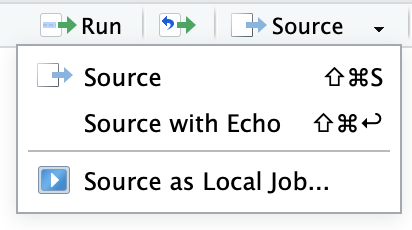
\includegraphics[width=0.35\linewidth]{ch_introduction/images/screenshot_source} \caption{Source button options}\label{fig:sourcebutton}
\end{figure}

\subsection{Run select text}\label{run-select-text}

The Run button will run the text you highlight and present the relevant output. You have used this command a fair amount already.

I strongly suggest you ONLY use the Run button when testing a command to make sure it works or to debug a script. Or to run library(tidyverse) as you start working on your script so that you get the autocomplete options.

In general, you should always try to execute your R Scripts using the Source with Echo command (preceded by a Restart, see below). This ensures your script will work beginning to end for you in the future and for others that attempt to use it. Using the Run button in an ad lib basis can create output that is not reproducible.

\subsection{Source (without Echo)}\label{source-without-echo}

Source (without Echo) is not designed for the typical analysis workflow. It is mostly helpful when you run simulations. When you run Source (without Echo) much of the output you would wish to read is suppressed. In general, avoid this option. If you use it, you often won't see what you want to see in the output.

\subsection{Source with Echo}\label{source-with-echo}

The Source with Echo command runs all of the contents of a script and presents the output in the R console. This is the approach you should use to running your scripts in most cases.

Prior to running Source with Echo (or just Source), it's always a good idea to restart R. This makes sure you clear the computer memory of any errors from any previous runs.

So you should do the following EVERY time you run your script.

\begin{enumerate}
\def\labelenumi{\arabic{enumi}.}
\tightlist
\item
  Use the menu item: \textbf{Session \textgreater{} Restart R}
\item
  Click the down arrow beside the Source button, and click on Source With Echo
\end{enumerate}

This will clear potentially problematic previous stats, run the script commands, and display the output in the Console. Moving forward we will use this approach for running scripts. Once you have used Source with Echo once, you can just click the Source button and it will use Source with Echo automatically (without the need to use the pull down option for selecting Source with Echo).

\begin{rmdcaution}
Using Restart R before you run a script, or R code in general, is a critical workflow tip.
\end{rmdcaution}

\section{Trying Source with Echo}\label{trying-source-with-echo}

Put the head(), tail(), and summary() command we used previously into your script. Then save your script using using the File \textgreater{} Save menu. You script should appear as below.

\begin{Shaded}
\begin{Highlighting}[]
\CommentTok{\# Code written on: YYYY/MM/DD }
\CommentTok{\# By: John Smith}
\FunctionTok{library}\NormalTok{(tidyverse)}

\NormalTok{okcupid\_profiles }\OtherTok{\textless{}{-}} \FunctionTok{read\_csv}\NormalTok{(}\AttributeTok{file =} \StringTok{"data\_okcupid.csv"}\NormalTok{)}

\FunctionTok{head}\NormalTok{(okcupid\_profiles)}

\FunctionTok{tail}\NormalTok{(okcupid\_profiles)}

\FunctionTok{summary}\NormalTok{(okcupid\_profiles)}
\end{Highlighting}
\end{Shaded}

Now do the following:

\begin{enumerate}
\def\labelenumi{\arabic{enumi}.}
\tightlist
\item
  Use the menu item: \textbf{Session \textgreater{} Restart R}
\item
  Click the down arrow beside the Source button, and click on Source With Echo
\end{enumerate}

You should see the output below:

\begin{Shaded}
\begin{Highlighting}[]
\CommentTok{\# Code written on: YYYY/MM/DD }
\CommentTok{\# By: John Smith}
\FunctionTok{library}\NormalTok{(tidyverse)}

\NormalTok{okcupid\_profiles }\OtherTok{\textless{}{-}} \FunctionTok{read\_csv}\NormalTok{(}\AttributeTok{file =} \StringTok{"data\_okcupid.csv"}\NormalTok{)}
\end{Highlighting}
\end{Shaded}

\begin{verbatim}
## Rows: 59946 Columns: 6
## -- Column specification ----------------------------------------------------------
## Delimiter: ","
## chr (4): diet, pets, sex, status
## dbl (2): age, height
## 
## i Use `spec()` to retrieve the full column specification for this data.
## i Specify the column types or set `show_col_types = FALSE` to quiet this message.
\end{verbatim}

\begin{Shaded}
\begin{Highlighting}[]
\FunctionTok{head}\NormalTok{(okcupid\_profiles)}
\end{Highlighting}
\end{Shaded}

\begin{verbatim}
## # A tibble: 6 x 6
##     age diet              height pets           sex   status
##   <dbl> <chr>              <dbl> <chr>          <chr> <chr> 
## 1    22 strictly anything     75 likes dogs an~ m     single
## 2    35 mostly other          70 likes dogs an~ m     single
## 3    38 anything              68 has cats       m     avail~
## 4    23 vegetarian            71 likes cats     m     single
## 5    29 <NA>                  66 likes dogs an~ m     single
## 6    29 mostly anything       67 likes cats     m     single
\end{verbatim}

\begin{Shaded}
\begin{Highlighting}[]
\FunctionTok{tail}\NormalTok{(okcupid\_profiles)}
\end{Highlighting}
\end{Shaded}

\begin{verbatim}
## # A tibble: 6 x 6
##     age diet            height pets             sex   status
##   <dbl> <chr>            <dbl> <chr>            <chr> <chr> 
## 1    31 <NA>                62 likes dogs       f     single
## 2    59 <NA>                62 has dogs         f     single
## 3    24 mostly anything     72 likes dogs and ~ m     single
## 4    42 mostly anything     71 <NA>             m     single
## 5    27 mostly anything     73 likes dogs and ~ m     single
## 6    39 <NA>                68 likes dogs and ~ m     single
\end{verbatim}

\begin{Shaded}
\begin{Highlighting}[]
\FunctionTok{summary}\NormalTok{(okcupid\_profiles)}
\end{Highlighting}
\end{Shaded}

\begin{verbatim}
##       age            diet               height    
##  Min.   : 18.0   Length:59946       Min.   : 1.0  
##  1st Qu.: 26.0   Class :character   1st Qu.:66.0  
##  Median : 30.0   Mode  :character   Median :68.0  
##  Mean   : 32.3                      Mean   :68.3  
##  3rd Qu.: 37.0                      3rd Qu.:71.0  
##  Max.   :110.0                      Max.   :95.0  
##                                     NA's   :3     
##      pets               sex               status         
##  Length:59946       Length:59946       Length:59946      
##  Class :character   Class :character   Class :character  
##  Mode  :character   Mode  :character   Mode  :character  
##                                                          
##                                                          
##                                                          
## 
\end{verbatim}

Congratulations you just ran your first script!

\section{A few key points about}\label{a-few-key-points-about}

Sometimes you will need to send a command additional information. Moreover, that information often needs to be grouped together into a vector or a list before you can send it to the command. We'll learn more about doing so in the future but here is a quick over view of vectors and lists to provide a foundation for future chapters.

\subsubsection{Vector of numbers}\label{vector-of-numbers}

We can create a vector of only numbers using the ``c'' function - which you can think of as being short for ``combine'' (or concatenate). In the commands below we create a vector of a few even numbers called ``even\_numbers''.

\begin{Shaded}
\begin{Highlighting}[]
\NormalTok{even\_numbers }\OtherTok{\textless{}{-}} \FunctionTok{c}\NormalTok{(}\DecValTok{2}\NormalTok{, }\DecValTok{4}\NormalTok{, }\DecValTok{6}\NormalTok{, }\DecValTok{8}\NormalTok{, }\DecValTok{10}\NormalTok{)}
\end{Highlighting}
\end{Shaded}

\begin{Shaded}
\begin{Highlighting}[]
\FunctionTok{print}\NormalTok{(even\_numbers)}
\end{Highlighting}
\end{Shaded}

\begin{verbatim}
## [1]  2  4  6  8 10
\end{verbatim}

We can obtain the second number in the vector using the following notation:

\begin{Shaded}
\begin{Highlighting}[]
\FunctionTok{print}\NormalTok{(even\_numbers[}\DecValTok{2}\NormalTok{])}
\end{Highlighting}
\end{Shaded}

\begin{verbatim}
## [1] 4
\end{verbatim}

\subsubsection{Vector of characters}\label{vector-of-characters}

We can also create vectors using only characters. Note that I use \textbf{SHIFT RETURN} after each comma to move to the next line.

\begin{Shaded}
\begin{Highlighting}[]
\NormalTok{favourite\_things }\OtherTok{\textless{}{-}} \FunctionTok{c}\NormalTok{(}\StringTok{"copper kettles"}\NormalTok{,}
                      \StringTok{"woolen mittens"}\NormalTok{,}
                      \StringTok{"brown paper packages"}\NormalTok{)}
\end{Highlighting}
\end{Shaded}

\begin{Shaded}
\begin{Highlighting}[]
\FunctionTok{print}\NormalTok{(favourite\_things)}
\end{Highlighting}
\end{Shaded}

\begin{verbatim}
## [1] "copper kettles"       "woolen mittens"      
## [3] "brown paper packages"
\end{verbatim}

As before, can obtain the second item in the vector using the following notation:

\begin{Shaded}
\begin{Highlighting}[]
\FunctionTok{print}\NormalTok{(favourite\_things[}\DecValTok{2}\NormalTok{])}
\end{Highlighting}
\end{Shaded}

\begin{verbatim}
## [1] "woolen mittens"
\end{verbatim}

\subsection{Lists}\label{lists}

Lists are similar to vectors in that you can create them and access items by their numeric position. Vectors must be all characters or all numbers. Lists can be a mix of characters or numbers. Most importantly items in lists can be accessed by their label. Note that I use \textbf{SHIFT RETURN} after each comma to move to the next line in the code below.

\begin{Shaded}
\begin{Highlighting}[]
\NormalTok{my\_list }\OtherTok{\textless{}{-}} \FunctionTok{list}\NormalTok{(}\AttributeTok{last\_name =} \StringTok{"Smith"}\NormalTok{,}
                \AttributeTok{first\_name =} \StringTok{"John"}\NormalTok{,}
                \AttributeTok{office\_number =} \DecValTok{1913}\NormalTok{)}

\FunctionTok{print}\NormalTok{(my\_list)}
\end{Highlighting}
\end{Shaded}

\begin{verbatim}
## $last_name
## [1] "Smith"
## 
## $first_name
## [1] "John"
## 
## $office_number
## [1] 1913
\end{verbatim}

You can access an item in a list using double brackets:

\begin{Shaded}
\begin{Highlighting}[]
\FunctionTok{print}\NormalTok{(my\_list[}\DecValTok{2}\NormalTok{])}
\end{Highlighting}
\end{Shaded}

\begin{verbatim}
## $first_name
## [1] "John"
\end{verbatim}

You can access an item in a list by its label/name using the dollar sign:

\begin{Shaded}
\begin{Highlighting}[]
\FunctionTok{print}\NormalTok{(my\_list}\SpecialCharTok{$}\NormalTok{last\_name)}
\end{Highlighting}
\end{Shaded}

\begin{verbatim}
## [1] "Smith"
\end{verbatim}

\begin{Shaded}
\begin{Highlighting}[]
\FunctionTok{print}\NormalTok{(my\_list}\SpecialCharTok{$}\NormalTok{office\_number)}
\end{Highlighting}
\end{Shaded}

\begin{verbatim}
## [1] 1913
\end{verbatim}

\section{Revisiting read\_csv()}\label{revisiting-read_csv}

In the text above we learned about vectors of characters. This information can be used handle missing values in the read\_csv() command. Consider a data set where for many participants we did not get a response to a question. We might have that represented in various ways within the data file. The value for that question might simply be omitted (i.e., represented by nothing -- ``\,``), represented by NA for not available, or maybe simply be something like -777.

When we load data with read\_csv() we can indicate to the computer how missing values are represented. This ensures the computer sees something like -777 as a missing value rather than an actual value. We do so in the read\_csv() command below using the \textbf{na} argument (not available). Note: use SHIFT-RETURN or SHIFT-ENTER to move the next line within the read\_csv() command. Failure to indicate the missing value codes within read\_csv() will result in incorrect answers in most scenarios with missing data.

\begin{Shaded}
\begin{Highlighting}[]
\NormalTok{okcupid\_profiles }\OtherTok{\textless{}{-}} \FunctionTok{read\_csv}\NormalTok{(}\AttributeTok{file =} \StringTok{"data\_okcupid.csv"}\NormalTok{,}
                             \AttributeTok{na =} \FunctionTok{c}\NormalTok{(}\StringTok{""}\NormalTok{, }\StringTok{"NA"}\NormalTok{, }\StringTok{"{-}777"}\NormalTok{))}
\end{Highlighting}
\end{Shaded}

\section{That's it!}\label{thats-it}

Congratulations! You've reached the end of the introduction to R. Take a break, have a cookie, and read some more about R tomorrow!

\chapter{Handling Data with the Tidyverse}\label{handling-data-with-the-tidyverse}

A key component of doing statistics in the modern world is managing/wrangling or cleaning data to make it ready for analysis. Indeed, some estimate that those who do data science spend 80\% of their time engaged in cleaning data. Although this specific percentage \href{https://blog.ldodds.com/2020/01/31/do-data-scientists-spend-80-of-their-time-cleaning-data-turns-out-no/}{may not be accurate} it does accurately reflect the fact that data scientists do spend a substantial portion of their time preparing data for analysis. Many complain about this fact but as \href{https://blog.ldodds.com/2020/01/31/do-data-scientists-spend-80-of-their-time-cleaning-data-turns-out-no/}{Leigh Dodds} points out ``I would argue that spending time working with data. To transform, explore and understand it better is absolutely what data scientists should be doing. This is the medium they are working in.''

In this chapter we focus on teaching you foundational skills for data preparation. The skills taught in this chapter largely revolve around using the tidyverse packages to manage data that will eventually help with data cleaning in the \href{https://dstanley4.github.io/psyc6060bookdown/an-emphasis-on-workflow.html}{Workflow} and \href{https://dstanley4.github.io/psyc6060bookdown/qualtrics.html}{Qualtrics} chapters. There are some additional resources you may want to consult as you learn these tidyverse skills:

\begin{itemize}
\item
  \href{https://r4ds.had.co.nz}{R for Data Science book}. This is an excellent free online book! But it does reflect an exploratory analysis mindset compared to the confirmatory mindset we typically use in Psychological science.
\item
  You may find a \href{https://www.rstudio.com/resources/cheatsheets/}{cheatsheet} helpful. Specifically, the \href{https://rstudio.github.io/cheatsheets/data-transformation.pdf}{Data Transformation} cheatsheet.
\item
  \href{https://www.tidyverse.org}{tidyverse website}
\end{itemize}

\section{Required}\label{required}

The data files below are used in this chapter. Right click to save each file.

\begin{longtable}[]{@{}l@{}}
\toprule\noalign{}
Required Data \\
\midrule\noalign{}
\endhead
\bottomrule\noalign{}
\endlastfoot
\url{data_okcupid.csv} \\
\url{data_experiment.csv} \\
\end{longtable}

The following CRAN packages must be installed:

\begin{longtable}[]{@{}l@{}}
\toprule\noalign{}
Required CRAN Packages \\
\midrule\noalign{}
\endhead
\bottomrule\noalign{}
\endlastfoot
tidyverse \\
\end{longtable}

\section{Objective}\label{objective}

The objective of this chapter is to familiarize you with some key commands in the tidyverse. These commands are used in isolation of each other for the most part. In the next chapter we will use these commands in a more coordinated way as we load a data set and move it from raw data to data that is ready for analysis (i.e., analytic data). You can start this project by Starting the class assignment on R Studio Cloud that corresponds to the chapter name.

\section{Using the Console}\label{using-the-console}

All of the commands in this chapter should be typed into the Console within R. If you see a command split over multiple lines, use SHIFT-RETURN (macOS) or SHIFT-ENTER (Windows) to move the next line that is part of the same command.

\section{Basic tidyverse commands}\label{basic-tidyverse-commands}

If you inspect the Files tab on the lower-right panel in R Studio you will see the file data\_okcupid.csv. The code below loads that file. Recall you should type this code into the R Console.

\begin{Shaded}
\begin{Highlighting}[]
\FunctionTok{library}\NormalTok{(tidyverse)}
\NormalTok{okcupid\_profiles }\OtherTok{\textless{}{-}} \FunctionTok{read\_csv}\NormalTok{(}\StringTok{"data\_okcupid.csv"}\NormalTok{)}
\end{Highlighting}
\end{Shaded}

You can see the first few rows of the data using the print() command. Each row presents a person whereas each column represents a variable. If you have a large number of columns you will only see the first several columns with this approach to viewing your data.

\begin{Shaded}
\begin{Highlighting}[]
\FunctionTok{print}\NormalTok{(okcupid\_profiles)}
\end{Highlighting}
\end{Shaded}

\begin{verbatim}
## # A tibble: 59,946 x 6
##      age diet              height pets          sex   status
##    <dbl> <chr>              <dbl> <chr>         <chr> <chr> 
##  1    22 strictly anything     75 likes dogs a~ m     single
##  2    35 mostly other          70 likes dogs a~ m     single
##  3    38 anything              68 has cats      m     avail~
##  4    23 vegetarian            71 likes cats    m     single
##  5    29 <NA>                  66 likes dogs a~ m     single
##  6    29 mostly anything       67 likes cats    m     single
##  7    32 strictly anything     65 likes dogs a~ f     single
##  8    31 mostly anything       65 likes dogs a~ f     single
##  9    24 strictly anything     67 likes dogs a~ f     single
## 10    37 mostly anything       65 likes dogs a~ m     single
## # i 59,936 more rows
\end{verbatim}

But it's also helpful just to see a list of the columns in the data with the glimpse() command:

\begin{Shaded}
\begin{Highlighting}[]
\FunctionTok{glimpse}\NormalTok{(okcupid\_profiles)}
\end{Highlighting}
\end{Shaded}

\begin{verbatim}
## Rows: 59,946
## Columns: 6
## $ age    <dbl> 22, 35, 38, 23, 29, 29, 32, 31, 24, 37, 35,~
## $ diet   <chr> "strictly anything", "mostly other", "anyth~
## $ height <dbl> 75, 70, 68, 71, 66, 67, 65, 65, 67, 65, 70,~
## $ pets   <chr> "likes dogs and likes cats", "likes dogs an~
## $ sex    <chr> "m", "m", "m", "m", "m", "m", "f", "f", "f"~
## $ status <chr> "single", "single", "available", "single", ~
\end{verbatim}

The glimpse() command is useful because it quickly allows you to see all of the columns. Moreover, it allows you to see the type for each column. Types were briefly discussed in the last chapter. Notice in the output beside each column name that some columns are labeled ``dbl'' which is short for double -- a type of numeric column. Other columns are labeled ``chr'' which is short for character - meaning the columns contain characters. These designations will become important in the next chapter as we prepare data for analysis.

\subsection{decimals}\label{decimals}

Often the tidyverse doesn't show the desired number of digits - this means too few digits after each decimal. You can set the desired number of total digits (before/after the decimal) with the options(pillar.sigfig = 3) command. Three is the default - but probably too low for our purposes. We'll begin with this value of 3 but change it later to 6 in the summarise() section.

\begin{Shaded}
\begin{Highlighting}[]
\CommentTok{\#default value for digits}
\FunctionTok{options}\NormalTok{(}\AttributeTok{pillar.sigfig =} \DecValTok{3}\NormalTok{)}

\CommentTok{\#suggested value you set in your script at the top}
\FunctionTok{options}\NormalTok{(}\AttributeTok{pillar.sigfig =} \DecValTok{6}\NormalTok{)}
\end{Highlighting}
\end{Shaded}

\subsection{select()}\label{select}

The select() command allows you to obtain a subset of the columns in your data. The commands below can be used to obtain the age and height columns. You can read the command as: take the okcupid\_profiles data and then select the age and height columns. The ``\%\textgreater\%'' symbol can be read as ``and then''. You can see that this code prints out the data with just the age and height columns. Remember, use SHIFT-ENTER or SHIFT-RETURN to move to the next line in the block of code.

\begin{Shaded}
\begin{Highlighting}[]
\NormalTok{okcupid\_profiles }\SpecialCharTok{\%\textgreater{}\%} 
  \FunctionTok{select}\NormalTok{(age, height)}
\end{Highlighting}
\end{Shaded}

\begin{verbatim}
## # A tibble: 59,946 x 2
##      age height
##    <dbl>  <dbl>
##  1    22     75
##  2    35     70
##  3    38     68
##  4    23     71
##  5    29     66
##  6    29     67
##  7    32     65
##  8    31     65
##  9    24     67
## 10    37     65
## # i 59,936 more rows
\end{verbatim}

Of course, it's usually of little help to just print the subset of the data. It's better to store it in a new data. In the command below we store the resulting data in a new data set called new\_data.

\begin{Shaded}
\begin{Highlighting}[]
\NormalTok{new\_data }\OtherTok{\textless{}{-}}\NormalTok{ okcupid\_profiles }\SpecialCharTok{\%\textgreater{}\%} 
  \FunctionTok{select}\NormalTok{(age, height)}
\end{Highlighting}
\end{Shaded}

The glimpse() command shows us that only the age and height columns are in new\_data.

\begin{Shaded}
\begin{Highlighting}[]
\FunctionTok{glimpse}\NormalTok{(new\_data)}
\end{Highlighting}
\end{Shaded}

\begin{verbatim}
## Rows: 59,946
## Columns: 2
## $ age    <dbl> 22, 35, 38, 23, 29, 29, 32, 31, 24, 37, 35,~
## $ height <dbl> 75, 70, 68, 71, 66, 67, 65, 65, 67, 65, 70,~
\end{verbatim}

In the above example we indicated the columns we wanted to retain from the okcupid\_profiles data using the select() command. However, we can also indicate the columns we want to drop from okcupid\_profiles using a minus sign (-) in front of the columns we specify in the select() command.

\begin{Shaded}
\begin{Highlighting}[]
\NormalTok{new\_data }\OtherTok{\textless{}{-}}\NormalTok{ okcupid\_profiles }\SpecialCharTok{\%\textgreater{}\%} \FunctionTok{select}\NormalTok{(}\SpecialCharTok{{-}}\NormalTok{age, }\SpecialCharTok{{-}}\NormalTok{height)}
\end{Highlighting}
\end{Shaded}

The glimpse() command shows us that we kept all the columns except the age and height columns when we created new\_data.

\begin{Shaded}
\begin{Highlighting}[]
\FunctionTok{glimpse}\NormalTok{(new\_data)}
\end{Highlighting}
\end{Shaded}

\begin{verbatim}
## Rows: 59,946
## Columns: 4
## $ diet   <chr> "strictly anything", "mostly other", "anyth~
## $ pets   <chr> "likes dogs and likes cats", "likes dogs an~
## $ sex    <chr> "m", "m", "m", "m", "m", "m", "f", "f", "f"~
## $ status <chr> "single", "single", "available", "single", ~
\end{verbatim}

\subsection{summarise()}\label{summarise}

The summarise() command can be used to generate descriptive statistics for a specified column. You can easily calculate column descriptive statistics using the corresponding commands for mean(), sd(), min(), max(), among others. In the example below we calculate the mean for the age column.

In the code below, mean(age, na.rm = TRUE), indicates to R that it should calculate the mean of the age column. The na.rm indicates how missing values should be handled. The na stands for not available; in R missing values are classified as Not Available or NA. The rm stands for remove. Consequently, na.rm is asking: ``Should we remove missing values when calculating the mean?'' The TRUE indicates that yes, missing values should be removed when calculating the mean. The result of this calculation is placed into a variable labelled age\_mean, though we could have used any label we wanted instead of age\_mean. We see that the mean of the age column is, with rounding, 32.3.

\begin{Shaded}
\begin{Highlighting}[]
\NormalTok{okcupid\_profiles }\SpecialCharTok{\%\textgreater{}\%} 
  \FunctionTok{summarise}\NormalTok{(}\AttributeTok{age\_mean =} \FunctionTok{mean}\NormalTok{(age, }\AttributeTok{na.rm =} \ConstantTok{TRUE}\NormalTok{))}
\end{Highlighting}
\end{Shaded}

\begin{verbatim}
## # A tibble: 1 x 1
##   age_mean
##      <dbl>
## 1     32.3
\end{verbatim}

More than one calculation can occur in the same summarise() command. You can easily add the calculation for the standared deviation with the sd() command.

\begin{Shaded}
\begin{Highlighting}[]
\NormalTok{okcupid\_profiles }\SpecialCharTok{\%\textgreater{}\%} 
  \FunctionTok{summarise}\NormalTok{(}\AttributeTok{age\_mean =} \FunctionTok{mean}\NormalTok{(age, }\AttributeTok{na.rm =} \ConstantTok{TRUE}\NormalTok{),}
            \AttributeTok{age\_sd =} \FunctionTok{sd}\NormalTok{(age, }\AttributeTok{na.rm =} \ConstantTok{TRUE}\NormalTok{))}
\end{Highlighting}
\end{Shaded}

\begin{verbatim}
## # A tibble: 1 x 2
##   age_mean age_sd
##      <dbl>  <dbl>
## 1     32.3   9.45
\end{verbatim}

Often this process does too much rounding. We can get more exact results changing the number of decimals with the options(pillar.sigfig = 6) command before our analysis. See the difference below. Now we see more digits. I encourage you to sue this command at the top of your script. The default is options(pillar.sigfig = 3) I suggest you use options(pillar.sigfig = 6) or higher.

\begin{Shaded}
\begin{Highlighting}[]
\CommentTok{\#NOTICE: We have increased the number of digits in the output}
\FunctionTok{options}\NormalTok{(}\AttributeTok{pillar.sigfig =} \DecValTok{6}\NormalTok{)}

\NormalTok{okcupid\_profiles }\SpecialCharTok{\%\textgreater{}\%} 
  \FunctionTok{summarise}\NormalTok{(}\AttributeTok{age\_mean =} \FunctionTok{mean}\NormalTok{(age, }\AttributeTok{na.rm =} \ConstantTok{TRUE}\NormalTok{),}
            \AttributeTok{age\_sd =} \FunctionTok{sd}\NormalTok{(age, }\AttributeTok{na.rm =} \ConstantTok{TRUE}\NormalTok{))}
\end{Highlighting}
\end{Shaded}

\begin{verbatim}
## # A tibble: 1 x 2
##   age_mean  age_sd
##      <dbl>   <dbl>
## 1  32.3403 9.45278
\end{verbatim}

\subsection{filter()}\label{filter}

The filter() command allows you to obtain a subset of the rows in your data. In the example below we create a new data set with just the males from the original data.

Notice the structure of the original data below in the glimpse() output. There is a column called sex that uses m and f to indicate male and female, respectively. Also notice that there are 59946 rows in the okcupid\_profiles data.

\begin{Shaded}
\begin{Highlighting}[]
\FunctionTok{glimpse}\NormalTok{(okcupid\_profiles)}
\end{Highlighting}
\end{Shaded}

\begin{verbatim}
## Rows: 59,946
## Columns: 6
## $ age    <dbl> 22, 35, 38, 23, 29, 29, 32, 31, 24, 37, 35,~
## $ diet   <chr> "strictly anything", "mostly other", "anyth~
## $ height <dbl> 75, 70, 68, 71, 66, 67, 65, 65, 67, 65, 70,~
## $ pets   <chr> "likes dogs and likes cats", "likes dogs an~
## $ sex    <chr> "m", "m", "m", "m", "m", "m", "f", "f", "f"~
## $ status <chr> "single", "single", "available", "single", ~
\end{verbatim}

We use the filter command to select a subset of the rows based on the content of any column. In this case the sex column is used to obtain a subset of the rows; the rows with the value ``m'' are obtained. Notice the double equals sign is used to indicate ``equal to''. The reason a double equals sign is used here (instead of a single equals sign) is to distinguish it from the use of the single equals sign in the summarise command above. In the summarise command above, the single equal sign was used to indicate ``assign to''. That is, assign to age\_mean the mean of the column age after it is calculated. A single equals sign indicates ``assign to'' whereas a double equals sign indicates ``is equal to''.

\begin{Shaded}
\begin{Highlighting}[]
\NormalTok{okcupid\_males }\OtherTok{\textless{}{-}}\NormalTok{ okcupid\_profiles }\SpecialCharTok{\%\textgreater{}\%}
  \FunctionTok{filter}\NormalTok{(sex }\SpecialCharTok{==} \StringTok{"m"}\NormalTok{)}
\end{Highlighting}
\end{Shaded}

We use glimpse() to inspect these all male data. Notice that only the letter m is in the sex column - indicating only males are in the data set. Also notice that there are 35829 rows in the okcupid\_males data - fewer people because males are a subset of the total number of rows.

\begin{Shaded}
\begin{Highlighting}[]
\FunctionTok{glimpse}\NormalTok{(okcupid\_males)}
\end{Highlighting}
\end{Shaded}

\begin{verbatim}
## Rows: 35,829
## Columns: 6
## $ age    <dbl> 22, 35, 38, 23, 29, 29, 37, 35, 28, 24, 33,~
## $ diet   <chr> "strictly anything", "mostly other", "anyth~
## $ height <dbl> 75, 70, 68, 71, 66, 67, 65, 70, 72, 72, 70,~
## $ pets   <chr> "likes dogs and likes cats", "likes dogs an~
## $ sex    <chr> "m", "m", "m", "m", "m", "m", "m", "m", "m"~
## $ status <chr> "single", "single", "available", "single", ~
\end{verbatim}

The filter command can be combined with the summarise command to get the descriptive statistics for males without the hassle of creating new data. This is again done using the \%\textgreater\% ``and then'' operator.

\begin{Shaded}
\begin{Highlighting}[]
\NormalTok{okcupid\_profiles }\SpecialCharTok{\%\textgreater{}\%}
  \FunctionTok{filter}\NormalTok{(sex }\SpecialCharTok{==} \StringTok{"m"}\NormalTok{) }\SpecialCharTok{\%\textgreater{}\%}
  \FunctionTok{summarise}\NormalTok{(}\AttributeTok{age\_mean =} \FunctionTok{mean}\NormalTok{(age, }\AttributeTok{na.rm =} \ConstantTok{TRUE}\NormalTok{),}
            \AttributeTok{age\_sd =} \FunctionTok{sd}\NormalTok{(age, }\AttributeTok{na.rm =} \ConstantTok{TRUE}\NormalTok{))}
\end{Highlighting}
\end{Shaded}

\begin{verbatim}
## # A tibble: 1 x 2
##   age_mean  age_sd
##      <dbl>   <dbl>
## 1  32.0186 9.03288
\end{verbatim}

We see that for the 35829 males the mean age is 32.0 and the standard deviation is 9.0.

Likewise, we can obtain the descriptive statistics for females with only a slight modification, changing m to f in the filter command:

\begin{Shaded}
\begin{Highlighting}[]
\NormalTok{okcupid\_profiles }\SpecialCharTok{\%\textgreater{}\%}
  \FunctionTok{filter}\NormalTok{(sex }\SpecialCharTok{==} \StringTok{"f"}\NormalTok{) }\SpecialCharTok{\%\textgreater{}\%}
  \FunctionTok{summarise}\NormalTok{(}\AttributeTok{age\_mean =} \FunctionTok{mean}\NormalTok{(age, }\AttributeTok{na.rm =} \ConstantTok{TRUE}\NormalTok{),}
            \AttributeTok{age\_sd =} \FunctionTok{sd}\NormalTok{(age, }\AttributeTok{na.rm =} \ConstantTok{TRUE}\NormalTok{))}
\end{Highlighting}
\end{Shaded}

\begin{verbatim}
## # A tibble: 1 x 2
##   age_mean  age_sd
##      <dbl>   <dbl>
## 1  32.8182 10.0254
\end{verbatim}

We see that for the 24117 females the mean age is 32.8 and the standard deviation is 10.0.

\subsection{group\_by()}\label{group_by}

The process we used with the filter command would quickly become onerous if we had many subgroups for a column. Consequently, it's often better to use the group() command to calculate descriptive statistics for the levels (e.g., male/female) of a variable. By telling the computer to group\_by() sex the summarise command is run separately for every level of sex (i.e., m and f).

\begin{Shaded}
\begin{Highlighting}[]
\NormalTok{okcupid\_profiles }\SpecialCharTok{\%\textgreater{}\%}
  \FunctionTok{group\_by}\NormalTok{(sex) }\SpecialCharTok{\%\textgreater{}\%}
  \FunctionTok{summarise}\NormalTok{(}\AttributeTok{age\_mean =} \FunctionTok{mean}\NormalTok{(age, }\AttributeTok{na.rm =} \ConstantTok{TRUE}\NormalTok{),}
            \AttributeTok{age\_sd =} \FunctionTok{sd}\NormalTok{(age, }\AttributeTok{na.rm =} \ConstantTok{TRUE}\NormalTok{)) }
\end{Highlighting}
\end{Shaded}

\begin{verbatim}
## # A tibble: 2 x 3
##   sex   age_mean   age_sd
##   <chr>    <dbl>    <dbl>
## 1 f      32.8182 10.0254 
## 2 m      32.0186  9.03288
\end{verbatim}

Fortunately, it's possible to use more than one grouping variable with the group\_by() command. In the code below we group by sex and status (i.e., dating status).

\begin{Shaded}
\begin{Highlighting}[]
\NormalTok{okcupid\_profiles }\SpecialCharTok{\%\textgreater{}\%}
  \FunctionTok{group\_by}\NormalTok{(sex, status) }\SpecialCharTok{\%\textgreater{}\%}
  \FunctionTok{summarise}\NormalTok{(}\AttributeTok{age\_mean =} \FunctionTok{mean}\NormalTok{(age, }\AttributeTok{na.rm =} \ConstantTok{TRUE}\NormalTok{),}
            \AttributeTok{age\_sd =} \FunctionTok{sd}\NormalTok{(age, }\AttributeTok{na.rm =} \ConstantTok{TRUE}\NormalTok{)) }
\end{Highlighting}
\end{Shaded}

\begin{verbatim}
## `summarise()` has grouped output by 'sex'. You can override using the `.groups`
## argument.
\end{verbatim}

\begin{verbatim}
## # A tibble: 10 x 4
## # Groups:   sex [2]
##    sex   status         age_mean   age_sd
##    <chr> <chr>             <dbl>    <dbl>
##  1 f     available       32.2378  8.53559
##  2 f     married         33.7111  8.13493
##  3 f     seeing someone  28.0748  6.44038
##  4 f     single          33.0440 10.1549 
##  5 f     unknown         27.75    5.90903
##  6 m     available       34.7543  9.40181
##  7 m     married         38.68   10.0785 
##  8 m     seeing someone  30.8115  7.06094
##  9 m     single          31.9214  9.03813
## 10 m     unknown         40.6667  8.86942
\end{verbatim}

The resulting output provide for age the mean and standard deviation for every combination of sex and dating status. The first five rows provide output for females at every level of dating status whereas the subsequent five rows provide output for males at every level of dating status.

\subsection{mutate()}\label{mutate}

The mutate() command can be used to calculate a new column in a data. In the example below we calculate a new column called age\_centered which is the new version of the age\_column where the mean of the column has been removed from every value. This is merely an example of the many different types of calculations we can perform to create a new column using mutate().

\begin{Shaded}
\begin{Highlighting}[]
\NormalTok{okcupid\_profiles }\OtherTok{\textless{}{-}}\NormalTok{ okcupid\_profiles }\SpecialCharTok{\%\textgreater{}\%}
  \FunctionTok{mutate}\NormalTok{(}\AttributeTok{age\_centered =}\NormalTok{ age }\SpecialCharTok{{-}} \FunctionTok{mean}\NormalTok{(age, }\AttributeTok{na.rm =} \ConstantTok{TRUE}\NormalTok{))}
\end{Highlighting}
\end{Shaded}

Notice that the glimpse() command reveals that after we use the mutate() command there is a new column called age\_centered.

\begin{Shaded}
\begin{Highlighting}[]
\FunctionTok{glimpse}\NormalTok{(okcupid\_profiles)}
\end{Highlighting}
\end{Shaded}

\begin{verbatim}
## Rows: 59,946
## Columns: 7
## $ age          <dbl> 22, 35, 38, 23, 29, 29, 32, 31, 24, 3~
## $ diet         <chr> "strictly anything", "mostly other", ~
## $ height       <dbl> 75, 70, 68, 71, 66, 67, 65, 65, 67, 6~
## $ pets         <chr> "likes dogs and likes cats", "likes d~
## $ sex          <chr> "m", "m", "m", "m", "m", "m", "f", "f~
## $ status       <chr> "single", "single", "available", "sin~
## $ age_centered <dbl> -10.3403, 2.6597, 5.6597, -9.3403, -3~
\end{verbatim}

\section{Advanced tidyverse commands}\label{advanced-tidyverse-commands}

In this advanced selection we revisit the commands from the basic tidyverse section but use more complicated code to either select or apply an action to more than one column at a time. We will indicate the columns that we want to select or apply an action to using: starts\_with(), ends\_with(), contains(), matches(), or where(). The first four of these are used to indicate columns based on column names. In contrast, the last command, where(), is used to indicate the columns based on the column type (numeric, character, factor, etc.).

We will review all five commands for indicating the columns we want in the select() selection below. Following that we will, for brevity, typically use only one of the five commands when illustrating how they work with summarise() and mutate().

We begin by loading a new data.

\begin{Shaded}
\begin{Highlighting}[]
\FunctionTok{library}\NormalTok{(tidyverse)}
\NormalTok{data\_exp }\OtherTok{\textless{}{-}} \FunctionTok{read\_csv}\NormalTok{(}\StringTok{"data\_experiment.csv"}\NormalTok{)}
\end{Highlighting}
\end{Shaded}

\begin{verbatim}
## Rows: 6 Columns: 6
## -- Column specification ----------------------------------------------------------
## Delimiter: ","
## chr (1): sex
## dbl (5): id, t1_vomit, t1_aggression, t2_vomit, t2_aggre...
## 
## i Use `spec()` to retrieve the full column specification for this data.
## i Specify the column types or set `show_col_types = FALSE` to quiet this message.
\end{verbatim}

The glimpse() command reveals that this is a small data set where every row represents one rat. The sex of the rat is recorded as well as, for each of two time points, a rating of vomiting and aggression.

\begin{Shaded}
\begin{Highlighting}[]
\FunctionTok{glimpse}\NormalTok{(data\_exp)}
\end{Highlighting}
\end{Shaded}

\begin{verbatim}
## Rows: 6
## Columns: 6
## $ id            <dbl> 1, 2, 3, 4, 5, 6
## $ sex           <chr> "male", "female", "male", "female", ~
## $ t1_vomit      <dbl> 3, 2, 0, 3, 2, 1
## $ t1_aggression <dbl> 5, 6, 4, 7, 3, 8
## $ t2_vomit      <dbl> 2, 1, 1, 2, 1, 2
## $ t2_aggression <dbl> 6, 7, 6, 7, 5, 8
\end{verbatim}

\subsection{select()}\label{select-1}

\subsubsection{select() using column name}\label{select-using-column-name}

\paragraph{starts\_with()}\label{starts_with}

starts\_with() allows us to select columns based on how the column name begins. Here we put the columns that begin with ``t1'' into a new data called data\_time1.

\begin{Shaded}
\begin{Highlighting}[]
\NormalTok{data\_time1 }\OtherTok{\textless{}{-}}\NormalTok{ data\_exp }\SpecialCharTok{\%\textgreater{}\%} 
  \FunctionTok{select}\NormalTok{(}\FunctionTok{starts\_with}\NormalTok{(}\StringTok{"t1"}\NormalTok{))}
\end{Highlighting}
\end{Shaded}

The glimpse command shows us the new data only contains the columns that begin with ``t1''

\begin{Shaded}
\begin{Highlighting}[]
\FunctionTok{glimpse}\NormalTok{(data\_time1)}
\end{Highlighting}
\end{Shaded}

\begin{verbatim}
## Rows: 6
## Columns: 2
## $ t1_vomit      <dbl> 3, 2, 0, 3, 2, 1
## $ t1_aggression <dbl> 5, 6, 4, 7, 3, 8
\end{verbatim}

\paragraph{ends\_with()}\label{ends_with}

ends\_with() allows us to select columns based on how the column name ends. Here we put the columns that end with ``aggression'' into a new data set called data\_aggression.

\begin{Shaded}
\begin{Highlighting}[]
\NormalTok{data\_aggression }\OtherTok{\textless{}{-}}\NormalTok{ data\_exp }\SpecialCharTok{\%\textgreater{}\%} 
  \FunctionTok{select}\NormalTok{(}\FunctionTok{ends\_with}\NormalTok{(}\StringTok{"aggression"}\NormalTok{))}
\end{Highlighting}
\end{Shaded}

\begin{Shaded}
\begin{Highlighting}[]
\FunctionTok{glimpse}\NormalTok{(data\_aggression)}
\end{Highlighting}
\end{Shaded}

\begin{verbatim}
## Rows: 6
## Columns: 2
## $ t1_aggression <dbl> 5, 6, 4, 7, 3, 8
## $ t2_aggression <dbl> 6, 7, 6, 7, 5, 8
\end{verbatim}

\paragraph{contains()}\label{contains}

contains() allows us to select columns based on the contents of the column name. Here we put the columns that have ``\_'' in the name into a new data set called new\_data.

\begin{Shaded}
\begin{Highlighting}[]
\NormalTok{new\_data }\OtherTok{\textless{}{-}}\NormalTok{ data\_exp }\SpecialCharTok{\%\textgreater{}\%} 
  \FunctionTok{select}\NormalTok{(}\FunctionTok{contains}\NormalTok{(}\StringTok{"\_"}\NormalTok{))}
\end{Highlighting}
\end{Shaded}

\begin{Shaded}
\begin{Highlighting}[]
\FunctionTok{glimpse}\NormalTok{(new\_data)}
\end{Highlighting}
\end{Shaded}

\begin{verbatim}
## Rows: 6
## Columns: 4
## $ t1_vomit      <dbl> 3, 2, 0, 3, 2, 1
## $ t1_aggression <dbl> 5, 6, 4, 7, 3, 8
## $ t2_vomit      <dbl> 2, 1, 1, 2, 1, 2
## $ t2_aggression <dbl> 6, 7, 6, 7, 5, 8
\end{verbatim}

\paragraph{matches()}\label{matches}

It's also possible to use \emph{regex} (i.e., a \emph{regular expression}) to select columns. Regex is a powerful way to specify search/matching requirements for text - in this case the text of column names. An explanation of regex is beyond the scope of this chapter. Nonetheless the example below uses regex to select any column with an underscore in the column name followed by any character. The result is the same as the above for the contains() command. However, the matches() command is more flexible than the contains() command and can take into account substantially more complicated situations.

\begin{Shaded}
\begin{Highlighting}[]
\NormalTok{data\_matched }\OtherTok{\textless{}{-}}\NormalTok{ data\_exp }\SpecialCharTok{\%\textgreater{}\%} 
  \FunctionTok{select}\NormalTok{(}\FunctionTok{matches}\NormalTok{(}\StringTok{"(\_.)"}\NormalTok{))}
\end{Highlighting}
\end{Shaded}

You can see the columns selected using regex:

\begin{Shaded}
\begin{Highlighting}[]
\FunctionTok{glimpse}\NormalTok{(data\_matched)}
\end{Highlighting}
\end{Shaded}

\begin{verbatim}
## Rows: 6
## Columns: 4
## $ t1_vomit      <dbl> 3, 2, 0, 3, 2, 1
## $ t1_aggression <dbl> 5, 6, 4, 7, 3, 8
## $ t2_vomit      <dbl> 2, 1, 1, 2, 1, 2
## $ t2_aggression <dbl> 6, 7, 6, 7, 5, 8
\end{verbatim}

You can learn about regex at \href{https://regexone.com}{RegexOne} and test your regex specification at \href{https://regex101.com}{Regex101}. Ideally though, as we discuss in the next chapter, you can use naming conventions that are sufficiently thoughtful that you don't need regex, or only rarely. The reason for this is that regex can be challenging to use. As Twitter user @ThatJenPerson noted ``Regex is like tequila: use it to try to solve a problem and now you have two problems.'' Nonetheless, at one or two points in the future we will use regex to solve a problem (but not tequila).

\subsubsection{select() using column type}\label{select-using-column-type}

In many cases we will want to select or perform an action on a column based on whether the column is a numeric, character, or factor column (indicated in glimpse output as dbl, chr, and fct, respectively). We will learn more about factors later in this chapter. Each of these column types can be selected by using is.numeric, is.character, or is.factor, respectively, in combination with the where() command.

We can select numeric columns using where() and is.numeric:

\begin{Shaded}
\begin{Highlighting}[]
\NormalTok{data\_numeric\_columns }\OtherTok{\textless{}{-}}\NormalTok{ data\_exp }\SpecialCharTok{\%\textgreater{}\%} 
  \FunctionTok{select}\NormalTok{(}\FunctionTok{where}\NormalTok{(is.numeric))}
\end{Highlighting}
\end{Shaded}

You can see the new data contains only the numeric columns:

\begin{Shaded}
\begin{Highlighting}[]
\FunctionTok{glimpse}\NormalTok{(data\_numeric\_columns)}
\end{Highlighting}
\end{Shaded}

\begin{verbatim}
## Rows: 6
## Columns: 5
## $ id            <dbl> 1, 2, 3, 4, 5, 6
## $ t1_vomit      <dbl> 3, 2, 0, 3, 2, 1
## $ t1_aggression <dbl> 5, 6, 4, 7, 3, 8
## $ t2_vomit      <dbl> 2, 1, 1, 2, 1, 2
## $ t2_aggression <dbl> 6, 7, 6, 7, 5, 8
\end{verbatim}

We can select character (i.e., chr) columns using where() and is.character:

\begin{Shaded}
\begin{Highlighting}[]
\NormalTok{data\_character\_columns }\OtherTok{\textless{}{-}}\NormalTok{ data\_exp }\SpecialCharTok{\%\textgreater{}\%} 
  \FunctionTok{select}\NormalTok{(}\FunctionTok{where}\NormalTok{(is.character))}
\end{Highlighting}
\end{Shaded}

You can see the new data contains only the character columns:

\begin{Shaded}
\begin{Highlighting}[]
\FunctionTok{glimpse}\NormalTok{(data\_character\_columns)}
\end{Highlighting}
\end{Shaded}

\begin{verbatim}
## Rows: 6
## Columns: 1
## $ sex <chr> "male", "female", "male", "female", "male", "f~
\end{verbatim}

In a future chapter you will see how we can select factors using the where() command.

\subsection{summarise()}\label{summarise-1}

The summarise() command can summarise multiple columns when combined with starts\_with(), ends\_with(), contains(), matches(), and where(). However, to use these powerful tools for indicating columns with the summarise command we need the help of the across() command (i.e., across multiple columns).

If we want to obtain the mean of all the columns that start with ``t1'' we use the commands below. The across command requires that we indicate the columns we want via the .cols argument and the command/function we want to run on those columns via the .fns argument. In the example below, we also add na.rm = TRUE at the end; this is something we send to the mean command to let it know how we want to handle missing data.

\begin{Shaded}
\begin{Highlighting}[]
\NormalTok{data\_exp }\SpecialCharTok{\%\textgreater{}\%}
  \FunctionTok{summarise}\NormalTok{(}\FunctionTok{across}\NormalTok{(}\AttributeTok{.cols =} \FunctionTok{starts\_with}\NormalTok{(}\StringTok{"t1"}\NormalTok{), }
                   \AttributeTok{.fns =}\NormalTok{ \textbackslash{}(x) }\FunctionTok{mean}\NormalTok{(x, }\AttributeTok{na.rm =} \ConstantTok{TRUE}\NormalTok{)))}
\end{Highlighting}
\end{Shaded}

\begin{verbatim}
## # A tibble: 1 x 2
##   t1_vomit t1_aggression
##      <dbl>         <dbl>
## 1  1.83333           5.5
\end{verbatim}

If you want to get more sophisticated, you can also add this .names argument below which tells R to call label each output mean by the column name followed by ``\_mean''.

\begin{Shaded}
\begin{Highlighting}[]
\NormalTok{data\_exp }\SpecialCharTok{\%\textgreater{}\%}
  \FunctionTok{summarise}\NormalTok{(}\FunctionTok{across}\NormalTok{(}\AttributeTok{.cols =} \FunctionTok{starts\_with}\NormalTok{(}\StringTok{"t1"}\NormalTok{), }
                   \AttributeTok{.fns =}\NormalTok{ \textbackslash{}(x) }\FunctionTok{mean}\NormalTok{(x, }\AttributeTok{na.rm =} \ConstantTok{TRUE}\NormalTok{))) }
\end{Highlighting}
\end{Shaded}

\begin{verbatim}
## # A tibble: 1 x 2
##   t1_vomit t1_aggression
##      <dbl>         <dbl>
## 1  1.83333           5.5
\end{verbatim}

Often you want to calculate more than one statistic for each column. For example, you might want the mean, standard deviation, min, and max. These statistics can be calculated via the mean, sd, min, and max commands, respectively. However, you need to create a list with the statistics you desire.

Below we create a list of the descriptive statistics we desire called desired\_statistics, but you can use any name you want. This list only needs to be specified once, but we will repeat it in the examples below for clarity.

\begin{Shaded}
\begin{Highlighting}[]
\NormalTok{desired\_descriptives }\OtherTok{\textless{}{-}} \FunctionTok{list}\NormalTok{(}
  \AttributeTok{mean =} \SpecialCharTok{\textasciitilde{}}\FunctionTok{mean}\NormalTok{(.x, }\AttributeTok{na.rm =} \ConstantTok{TRUE}\NormalTok{),}
  \AttributeTok{sd =} \SpecialCharTok{\textasciitilde{}}\FunctionTok{sd}\NormalTok{(.x, }\AttributeTok{na.rm =} \ConstantTok{TRUE}\NormalTok{)}
\NormalTok{)}
\end{Highlighting}
\end{Shaded}

Once you have created the list of descriptive statistics you want you can run the command below to obtain those statistics. However, as you will see the output is too wide to be helpful.

\begin{Shaded}
\begin{Highlighting}[]
\NormalTok{data\_exp }\SpecialCharTok{\%\textgreater{}\%}
  \FunctionTok{summarise}\NormalTok{(}\FunctionTok{across}\NormalTok{(}\AttributeTok{.cols =} \FunctionTok{starts\_with}\NormalTok{(}\StringTok{"t1"}\NormalTok{), }
                   \AttributeTok{.fns =}\NormalTok{ desired\_descriptives)) }
\end{Highlighting}
\end{Shaded}

\begin{verbatim}
## # A tibble: 1 x 4
##   t1_vomit_mean t1_vomit_sd t1_aggression_mean
##           <dbl>       <dbl>              <dbl>
## 1       1.83333     1.16905                5.5
## # i 1 more variable: t1_aggression_sd <dbl>
\end{verbatim}

Consequently, we add the t() command (i.e., transpose command) to the end of the summarise request to get a more readable list of statistics:

\begin{Shaded}
\begin{Highlighting}[]
\NormalTok{desired\_descriptives }\OtherTok{\textless{}{-}} \FunctionTok{list}\NormalTok{(}
  \AttributeTok{mean =} \SpecialCharTok{\textasciitilde{}}\FunctionTok{mean}\NormalTok{(.x, }\AttributeTok{na.rm =} \ConstantTok{TRUE}\NormalTok{),}
  \AttributeTok{sd =} \SpecialCharTok{\textasciitilde{}}\FunctionTok{sd}\NormalTok{(.x, }\AttributeTok{na.rm =} \ConstantTok{TRUE}\NormalTok{)}
\NormalTok{)}

\NormalTok{data\_exp }\SpecialCharTok{\%\textgreater{}\%}
  \FunctionTok{summarise}\NormalTok{(}\FunctionTok{across}\NormalTok{(}\AttributeTok{.cols =} \FunctionTok{starts\_with}\NormalTok{(}\StringTok{"t1"}\NormalTok{), }
                   \AttributeTok{.fns =}\NormalTok{ desired\_descriptives)) }\SpecialCharTok{\%\textgreater{}\%}
  \FunctionTok{t}\NormalTok{() }
\end{Highlighting}
\end{Shaded}

\begin{verbatim}
##                     [,1]
## t1_vomit_mean      1.833
## t1_vomit_sd        1.169
## t1_aggression_mean 5.500
## t1_aggression_sd   1.871
\end{verbatim}

Note that in the across command above we could also have used: ends\_with(), contains(), matches(), or where().

\subsection{mutate()}\label{mutate-1}

The mutate() command can also be applied to multiple columns using the across() command. However, sometimes we need to embed our calculation in a custom function. Below is a custom function called make\_centered. This custom function takes the values in a column and subtracts the column mean from each value in the column. This is the same task we did previous using the mutate() command in the basic tidyverse section.

\begin{Shaded}
\begin{Highlighting}[]
\NormalTok{make\_centered }\OtherTok{\textless{}{-}} \ControlFlowTok{function}\NormalTok{(values) \{}
\NormalTok{  values\_out }\OtherTok{\textless{}{-}}\NormalTok{ values }\SpecialCharTok{{-}} \FunctionTok{mean}\NormalTok{(values, }\AttributeTok{na.rm =} \ConstantTok{TRUE}\NormalTok{)}
  \FunctionTok{return}\NormalTok{(values\_out)}
\NormalTok{\}}
\end{Highlighting}
\end{Shaded}

The glimpse() command shows us all the column names. Also notice the values in the agresssion columns are integers.

\begin{Shaded}
\begin{Highlighting}[]
\FunctionTok{glimpse}\NormalTok{(data\_exp)}
\end{Highlighting}
\end{Shaded}

\begin{verbatim}
## Rows: 6
## Columns: 6
## $ id            <dbl> 1, 2, 3, 4, 5, 6
## $ sex           <chr> "male", "female", "male", "female", ~
## $ t1_vomit      <dbl> 3, 2, 0, 3, 2, 1
## $ t1_aggression <dbl> 5, 6, 4, 7, 3, 8
## $ t2_vomit      <dbl> 2, 1, 1, 2, 1, 2
## $ t2_aggression <dbl> 6, 7, 6, 7, 5, 8
\end{verbatim}

We combine the mutate() command, with the across() command, and our custom make\_centered() command below. The command ``centers'' or subtracts the mean from any column that ends with ``aggression''.

\begin{Shaded}
\begin{Highlighting}[]
\NormalTok{data\_exp }\OtherTok{\textless{}{-}}\NormalTok{ data\_exp }\SpecialCharTok{\%\textgreater{}\%} 
  \FunctionTok{mutate}\NormalTok{(}\FunctionTok{across}\NormalTok{(}\AttributeTok{.cols =} \FunctionTok{ends\_with}\NormalTok{(}\StringTok{"aggression"}\NormalTok{), }
                \AttributeTok{.fns =}\NormalTok{ make\_centered))}
\end{Highlighting}
\end{Shaded}

You can see via the glimpse() output that the contents of all the columns that end with ``aggression'' have changed. Every value in each of these columns has had the column mean subtracted from it.

\begin{Shaded}
\begin{Highlighting}[]
\FunctionTok{glimpse}\NormalTok{(data\_exp)}
\end{Highlighting}
\end{Shaded}

\begin{verbatim}
## Rows: 6
## Columns: 6
## $ id            <dbl> 1, 2, 3, 4, 5, 6
## $ sex           <chr> "male", "female", "male", "female", ~
## $ t1_vomit      <dbl> 3, 2, 0, 3, 2, 1
## $ t1_aggression <dbl> -0.5, 0.5, -1.5, 1.5, -2.5, 2.5
## $ t2_vomit      <dbl> 2, 1, 1, 2, 1, 2
## $ t2_aggression <dbl> -0.5, 0.5, -0.5, 0.5, -1.5, 1.5
\end{verbatim}

Note that in the across() command above, we could also have used: starts\_with(), contains(), matches(), or where().

\subsubsection{mutate() within rows}\label{mutate-within-rows}

Researchers often want to average within rows and across columns to create a new column. That is, for each participant (i.e., rat in the current data) we might want to calculate a vomit score that is the average of the two time points (that we will call vomit\_avg).

To average within rows (and across columns) we use the rowwise() command to inform R of our intent. However, after we do the necessary calculations we have to shut off the rowwise() calculation state by using the ungroup() command. As well, when we are averaging within rows we have to use c\_across() instead of across(). The commands below create a new column called vomit\_avg which is the average of the vomit ratings across both times. As before, we also include na.rm = TRUE so the computer drops missing values (if present) when calculating the mean.

\begin{Shaded}
\begin{Highlighting}[]
\NormalTok{data\_exp }\OtherTok{\textless{}{-}}\NormalTok{ data\_exp }\SpecialCharTok{\%\textgreater{}\%} 
  \FunctionTok{rowwise}\NormalTok{() }\SpecialCharTok{\%\textgreater{}\%} 
  \FunctionTok{mutate}\NormalTok{(}\AttributeTok{vomit\_avg =} \FunctionTok{mean}\NormalTok{( }\FunctionTok{c\_across}\NormalTok{(}\AttributeTok{cols =} \FunctionTok{ends\_with}\NormalTok{(}\StringTok{"vomit"}\NormalTok{)),}
                           \AttributeTok{na.rm =} \ConstantTok{TRUE}\NormalTok{)) }\SpecialCharTok{\%\textgreater{}\%}
  \FunctionTok{ungroup}\NormalTok{()}
\end{Highlighting}
\end{Shaded}

You can see the new column we created with the glimpse() command:

\begin{Shaded}
\begin{Highlighting}[]
\FunctionTok{glimpse}\NormalTok{(data\_exp)}
\end{Highlighting}
\end{Shaded}

\begin{verbatim}
## Rows: 6
## Columns: 7
## $ id            <dbl> 1, 2, 3, 4, 5, 6
## $ sex           <chr> "male", "female", "male", "female", ~
## $ t1_vomit      <dbl> 3, 2, 0, 3, 2, 1
## $ t1_aggression <dbl> -0.5, 0.5, -1.5, 1.5, -2.5, 2.5
## $ t2_vomit      <dbl> 2, 1, 1, 2, 1, 2
## $ t2_aggression <dbl> -0.5, 0.5, -0.5, 0.5, -1.5, 1.5
## $ vomit_avg     <dbl> 2.5, 1.5, 0.5, 2.5, 1.5, 1.5
\end{verbatim}

The print() command could make it easier to see that the new column is the average of the other two, but if we use the print() command below it wouldn't work. Why? There are too many columns in the data set, so only the first few columns are shown.

\begin{Shaded}
\begin{Highlighting}[]
\FunctionTok{print}\NormalTok{(data\_exp)}
\end{Highlighting}
\end{Shaded}

To see that the new column, vomit\_avg, is the average of the other vomit columns we use the select command before print(). This prints only the relvant columns. When this is done, it's easy to see how the values in the vomit\_avg column are the mean of the other two columns.

\begin{Shaded}
\begin{Highlighting}[]
\NormalTok{data\_exp }\SpecialCharTok{\%\textgreater{}\%}
  \FunctionTok{select}\NormalTok{(}\FunctionTok{contains}\NormalTok{(}\StringTok{"vomit"}\NormalTok{)) }\SpecialCharTok{\%\textgreater{}\%}
  \FunctionTok{print}\NormalTok{()}
\end{Highlighting}
\end{Shaded}

\begin{verbatim}
## # A tibble: 6 x 3
##   t1_vomit t2_vomit vomit_avg
##      <dbl>    <dbl>     <dbl>
## 1        3        2       2.5
## 2        2        1       1.5
## 3        0        1       0.5
## 4        3        2       2.5
## 5        2        1       1.5
## 6        1        2       1.5
\end{verbatim}

\subsubsection{mutate() within rows using column names}\label{mutate-within-rows-using-column-names}

Sometimes it can be difficult to use one of the advanced select commands to obtain the columns you need to average across. The advanced commands like ends\_with() and starts\_with() can sometimes include columns you don't want. The command below is equivalent to the one above, however, we explicitly name the variables we want to average across.

\begin{Shaded}
\begin{Highlighting}[]
\NormalTok{data\_exp }\OtherTok{\textless{}{-}}\NormalTok{ data\_exp }\SpecialCharTok{\%\textgreater{}\%} 
  \FunctionTok{rowwise}\NormalTok{() }\SpecialCharTok{\%\textgreater{}\%} 
  \FunctionTok{mutate}\NormalTok{(}\AttributeTok{vomit\_avg =} \FunctionTok{mean}\NormalTok{( }\FunctionTok{c\_across}\NormalTok{(}\AttributeTok{cols =} \FunctionTok{c}\NormalTok{(t1\_vomit, t2\_vomit)),}
                           \AttributeTok{na.rm =} \ConstantTok{TRUE}\NormalTok{)) }\SpecialCharTok{\%\textgreater{}\%}
  \FunctionTok{ungroup}\NormalTok{()}
\end{Highlighting}
\end{Shaded}

You can use print() to confirm we get the same result:

\begin{Shaded}
\begin{Highlighting}[]
\NormalTok{data\_exp }\SpecialCharTok{\%\textgreater{}\%}
  \FunctionTok{select}\NormalTok{(}\FunctionTok{contains}\NormalTok{(}\StringTok{"vomit"}\NormalTok{)) }\SpecialCharTok{\%\textgreater{}\%}
  \FunctionTok{print}\NormalTok{()}
\end{Highlighting}
\end{Shaded}

\begin{verbatim}
## # A tibble: 6 x 3
##   t1_vomit t2_vomit vomit_avg
##      <dbl>    <dbl>     <dbl>
## 1        3        2       2.5
## 2        2        1       1.5
## 3        0        1       0.5
## 4        3        2       2.5
## 5        2        1       1.5
## 6        1        2       1.5
\end{verbatim}

\subsubsection{mutate() for factors}\label{mutate-for-factors}

It is critical that you indicate to R that categorical variables are in fact categorical variables. In R, categorical variables are referred to as factors. For humans, a factor like sex has three possible levels: female, male, intersex.

An inspection of the glimpse() command output reveals that the sex column has the type character - as indicated by ``chr''. Also notice, as you inspect this output, that we use words (e.g., female) to indicate the sex in the column rather than a number to represent a female participant (e.g., 2). This is the preferred, but less common, approach to entering data.

\begin{Shaded}
\begin{Highlighting}[]
\FunctionTok{glimpse}\NormalTok{(data\_exp)}
\end{Highlighting}
\end{Shaded}

\begin{verbatim}
## Rows: 6
## Columns: 7
## $ id            <dbl> 1, 2, 3, 4, 5, 6
## $ sex           <chr> "male", "female", "male", "female", ~
## $ t1_vomit      <dbl> 3, 2, 0, 3, 2, 1
## $ t1_aggression <dbl> -0.5, 0.5, -1.5, 1.5, -2.5, 2.5
## $ t2_vomit      <dbl> 2, 1, 1, 2, 1, 2
## $ t2_aggression <dbl> -0.5, 0.5, -0.5, 0.5, -1.5, 1.5
## $ vomit_avg     <dbl> 2.5, 1.5, 0.5, 2.5, 1.5, 1.5
\end{verbatim}

We need to convert the sex column to a factor in order for R to handle it appropriately in analyses. Failure to indicate the column is a factor column could result in R conducting all the analyses and presenting incorrect results. Consequently, it is critical that we covert the column to a factor. Fortunately, that is easily done using the as\_factor() command (there is also an as.factor command if as\_factor won't work for some reason).

We convert the sex column to a factor with this code:

\begin{Shaded}
\begin{Highlighting}[]
\NormalTok{data\_exp }\OtherTok{\textless{}{-}}\NormalTok{ data\_exp }\SpecialCharTok{\%\textgreater{}\%}
  \FunctionTok{mutate}\NormalTok{(}\AttributeTok{sex =} \FunctionTok{as\_factor}\NormalTok{(sex))}
\end{Highlighting}
\end{Shaded}

You can confirm this worked with the glimpse() command:

\begin{Shaded}
\begin{Highlighting}[]
\FunctionTok{glimpse}\NormalTok{(data\_exp)}
\end{Highlighting}
\end{Shaded}

\begin{verbatim}
## Rows: 6
## Columns: 7
## $ id            <dbl> 1, 2, 3, 4, 5, 6
## $ sex           <fct> male, female, male, female, male, fe~
## $ t1_vomit      <dbl> 3, 2, 0, 3, 2, 1
## $ t1_aggression <dbl> -0.5, 0.5, -1.5, 1.5, -2.5, 2.5
## $ t2_vomit      <dbl> 2, 1, 1, 2, 1, 2
## $ t2_aggression <dbl> -0.5, 0.5, -0.5, 0.5, -1.5, 1.5
## $ vomit_avg     <dbl> 2.5, 1.5, 0.5, 2.5, 1.5, 1.5
\end{verbatim}

If you entered your data using words for each level of sex (e.g., male, female) you're done at this point. However, if you used numbers to represent each level of sex in your data, there is one more step. Imagine your data was entered in a poorly advised manner, such that 1 was used to indicate male, 2 was used to indicate female, and 3 was used to indicate intersex. If this was the case, you need to indicate to R what each of those values represent. We do that with the code below.

\begin{Shaded}
\begin{Highlighting}[]
\NormalTok{data\_exp }\OtherTok{\textless{}{-}}\NormalTok{ data\_exp }\SpecialCharTok{\%\textgreater{}\%}
  \FunctionTok{mutate}\NormalTok{(}\AttributeTok{sex =} \FunctionTok{fct\_recode}\NormalTok{(sex,}
                          \AttributeTok{male =} \StringTok{"1"}\NormalTok{,}
                          \AttributeTok{female =} \StringTok{"2"}\NormalTok{,}
                          \AttributeTok{intersex =} \StringTok{"3"}\NormalTok{))}
\end{Highlighting}
\end{Shaded}

\section{Using help}\label{using-help}

In order to become efficient at analyzing data using R, you will need to become adapt at reading and understanding the help files associated with each command. After you have activated a package using the library command (e.g., library(tidyverse)) you can access the help page for every command in that package. To access the help page simply type a question mark followed by the command you want to know how to use (no space between them). The code below brings up the help page for the select() command. Notice that we put the library() command first - just a reminder that this needs to be done prior to using help for that package. Try the commands below in the Console:

\begin{Shaded}
\begin{Highlighting}[]
\FunctionTok{library}\NormalTok{(tidyverse)}
\NormalTok{?select}
\end{Highlighting}
\end{Shaded}

Examine the page that appears on the Help tab in the panel in the lower right of your screen. Read through the help file comparing what you read there to what we have learned about the select command. Notice how the help file tells you about the argument that you sent into the select() command, and also what the select() command returns when it receives those commands. Pay particular attention to the examples near the bottom of the help page. At the very bottom of the help page you will see {[}Package dplyr version 1.0.0 Index{]}. This tells you the select() command is from the dplyr package (part of the tidyverse). Notice that the word ``Index'' is underlined. Click on the word Index. You will be presented with list of other commands in the dplyr package.

As you become more experienced with R help pages, this is how you will learn to use new commands. Examine the help pages for the commands below by typing a question mark into the Console followed by the command name. Note that for filter and starts\_with you will be presented with a menu instead of help page. This typically occurs because the command is in more than one package. If this does occur, read through the options you are presented with to try and figure out which one you wanted. Typically, you want the first option. If you're not sure, try one. If it's not what you want, use the back arrow in the Help panel to go back and pick another one.

\begin{itemize}
\tightlist
\item
  mutate
\item
  filter
\item
  starts\_with
\end{itemize}

\section{Base R vs tidyverse}\label{base-r-vs-tidyverse}

All of the commands used to this point in the chapter have been the tidyverse approach to using R. That is the approach we will normally use. However, it's important to note that there is another way of using R, called base R.

Sometimes students have problems with their code when they mix and match these approaches using a bit of both. We will be using the tidyverse approach to using R but on the internet you will often see sample code that uses the older base R approach. A bit of background knowledge is helpful for understanding why we do things one way (e.g., read\_csv with the tidyverse) instead of another (e.g., read.csv with base R).

\subsection{Tibbles vs.~data frames}\label{tibbles-vs.-data-frames}

When you load data into R, it is typically represented in one of two formats inside the computer - depending on the command you used. The original format for representing a data set in R is the data frame. You will see this term used frequently when you read about R. When you load data using read.csv(), your data is loaded into a data frame in the computer. That is, your data is represented in the memory of the computer in a particular format and structure called a data frame. This contrasts with the newer tidyverse approach to representing data in the computer called a tibble - which is just a newer more advanced version of the data frame.

\subsection{read.csv() and data frames}\label{read.csv-and-data-frames}

When you read data into R using the command read.csv() (with a period) you load the data into a data frame (base R).

\begin{Shaded}
\begin{Highlighting}[]
\NormalTok{my\_dataframe }\OtherTok{\textless{}{-}} \FunctionTok{read.csv}\NormalTok{(}\AttributeTok{file =} \StringTok{"data\_okcupid.csv"}\NormalTok{)}
\end{Highlighting}
\end{Shaded}

Notice that when you print a data frame it does not show you the number of rows or columns above the data like our example did with the okcupid\_profiles data. Likewise, it does not show you the type of data in each column (e.g., dbl, fct, chr). It also presents all of your data rather than just the first few rows (as the tibble does). As a result, in the output below, we show only the first 10 rows of the output - because all the rows are printed in your Console with a data frame (too much to show here).

\begin{Shaded}
\begin{Highlighting}[]
\FunctionTok{print}\NormalTok{(my\_dataframe)}
\end{Highlighting}
\end{Shaded}

\begin{verbatim}
##    age              diet height                      pets
## 1   22 strictly anything     75 likes dogs and likes cats
## 2   35      mostly other     70 likes dogs and likes cats
## 3   38          anything     68                  has cats
## 4   23        vegetarian     71                likes cats
## 5   29              <NA>     66 likes dogs and likes cats
## 6   29   mostly anything     67                likes cats
## 7   32 strictly anything     65 likes dogs and likes cats
## 8   31   mostly anything     65 likes dogs and likes cats
## 9   24 strictly anything     67 likes dogs and likes cats
## 10  37   mostly anything     65 likes dogs and likes cats
##    sex    status
## 1    m    single
## 2    m    single
## 3    m available
## 4    m    single
## 5    m    single
## 6    m    single
## 7    f    single
## 8    f    single
## 9    f    single
## 10   m    single
\end{verbatim}

\subsection{read\_csv() and tibbles}\label{read_csv-and-tibbles}

When you read data into R using the command read\_csv() (with an underscore) you load the data into a tibble (tidyverse).

\begin{Shaded}
\begin{Highlighting}[]
\NormalTok{my\_tibble }\OtherTok{\textless{}{-}} \FunctionTok{read\_csv}\NormalTok{(}\AttributeTok{file =} \StringTok{"data\_okcupid.csv"}\NormalTok{)}
\end{Highlighting}
\end{Shaded}

\begin{verbatim}
## Rows: 59946 Columns: 6
## -- Column specification ----------------------------------------------------------
## Delimiter: ","
## chr (4): diet, pets, sex, status
## dbl (2): age, height
## 
## i Use `spec()` to retrieve the full column specification for this data.
## i Specify the column types or set `show_col_types = FALSE` to quiet this message.
\end{verbatim}

The tibble is modern version of the data frame. Notice that when you print a tibble it DOES show you the number of rows and columns. As well, it shows you the type of data in each column. Importantly, the tibble only provides the first few rows of output so it doesn't fill your screen.

\begin{Shaded}
\begin{Highlighting}[]
\FunctionTok{print}\NormalTok{(my\_tibble)}
\end{Highlighting}
\end{Shaded}

\begin{verbatim}
## # A tibble: 59,946 x 6
##      age diet              height pets          sex   status
##    <dbl> <chr>              <dbl> <chr>         <chr> <chr> 
##  1    22 strictly anything     75 likes dogs a~ m     single
##  2    35 mostly other          70 likes dogs a~ m     single
##  3    38 anything              68 has cats      m     avail~
##  4    23 vegetarian            71 likes cats    m     single
##  5    29 <NA>                  66 likes dogs a~ m     single
##  6    29 mostly anything       67 likes cats    m     single
##  7    32 strictly anything     65 likes dogs a~ f     single
##  8    31 mostly anything       65 likes dogs a~ f     single
##  9    24 strictly anything     67 likes dogs a~ f     single
## 10    37 mostly anything       65 likes dogs a~ m     single
## # i 59,936 more rows
\end{verbatim}

In short, you should always use tibbles (i.e., use read\_csv() not read.csv()). The differences between data frames and tibbles run deeper than the superficial output provided here. On some rare occasions an old package or command may not work with a tibble so you need to make it a data frame. You can do so with the commands below. We will flag these rare occurances to you when they occur.

\begin{Shaded}
\begin{Highlighting}[]
\CommentTok{\# Create a data frame from a tibble}
\NormalTok{new\_dataframe }\OtherTok{\textless{}{-}} \FunctionTok{as.data.frame}\NormalTok{(my\_tibble)}
\end{Highlighting}
\end{Shaded}

\chapter{Graphing}\label{graphing}

A great part of learning R is learning how to use ggplot2 which is part of the tidyverse. One way to learn ggplot2 is via the \href{https://ggplot2-book.org/index.html}{free ggplot book} - I encourage you to check it out. You might also check out this ggplot2 \href{https://rstudio.github.io/cheatsheets/data-visualization.pdf}{cheatsheet}. As well, you might consult this \href{https://tuowang.rbind.io/post/2021-04-25-color-in-ggplot2/}{blog} to learn more about how themes and colors are handled in ggplot2. In this chapter we merely provide a brief overview of how ggplot2 works. You can also consult this free book on \href{https://clauswilke.com/dataviz/}{data visualization techniques}.

\section{Required}\label{required-1}

The data files below are used in this chapter. Right click to save each file.

\begin{longtable}[]{@{}l@{}}
\toprule\noalign{}
Required Data \\
\midrule\noalign{}
\endhead
\bottomrule\noalign{}
\endlastfoot
\url{data_movies.csv} \\
\end{longtable}

The following packages CRAN must be installed:

\begin{longtable}[]{@{}l@{}}
\toprule\noalign{}
Required CRAN Packages \\
\midrule\noalign{}
\endhead
\bottomrule\noalign{}
\endlastfoot
tidyverse \\
RColorBrewer \\
remotes \\
\end{longtable}

The following GitHub packages must be installed:

\begin{longtable}[]{@{}l@{}}
\toprule\noalign{}
Required GitHub Packages \\
\midrule\noalign{}
\endhead
\bottomrule\noalign{}
\endlastfoot
dill/emoGG \\
\end{longtable}

After the remotes package is installed, it can be used to install a package from GitHub:

\begin{Shaded}
\begin{Highlighting}[]
\NormalTok{remotes}\SpecialCharTok{::}\FunctionTok{install\_github}\NormalTok{(}\StringTok{"dill/emoGG"}\NormalTok{)}
\end{Highlighting}
\end{Shaded}

\section{Data}\label{data}

To learn about making graphs using the tidyverse we use movie ratings and box office data obtained at the time of writing. Movie ratings were obtained from the \href{https://www.imdb.com}{IMDB} and \href{https://www.rottentomatoes.com}{RottenTomatoes}. Box office data (in millions of dollars) was obtained from \href{https://www.boxofficemojo.com}{Box Office Mojo}. If you enjoy learning about movies these are all excellent sites.

We begin by loading data\_movies.csv using read\_csv(), not read.csv():

\begin{Shaded}
\begin{Highlighting}[]
\NormalTok{movie\_data }\OtherTok{\textless{}{-}} \FunctionTok{read\_csv}\NormalTok{(}\StringTok{"data\_movies.csv"}\NormalTok{)}
\end{Highlighting}
\end{Shaded}

Next we inspect movie\_data using the print() command. We see that each row of the data set corresponds to a superhero movie.

\begin{Shaded}
\begin{Highlighting}[]
\FunctionTok{print}\NormalTok{(movie\_data)}
\end{Highlighting}
\end{Shaded}

\begin{verbatim}
## # A tibble: 8 x 7
##   title       short_title  year  imdb tomatoes_aud boxoffice
##   <chr>       <chr>       <dbl> <dbl>        <dbl>     <dbl>
## 1 Iron Man    Iron         2008   7.9           96       585
## 2 Thor Ragna~ Thor         2017   7.9           93       854
## 3 Avengers I~ AV3          2018   8.5           91      2048
## 4 Avengers E~ AV4          2019   8.7           91      2744
## 5 Man of Ste~ Sup          2013   7.1           75       668
## 6 Batman v S~ BvS          2015   6.5           63       873
## 7 Justice Le~ JL           2017   6.5           72       657
## 8 Wonder Wom~ WW           2017   7.5           88       821
## # i 1 more variable: studio <chr>
\end{verbatim}

Next we use glimpse() to see the columns.

\begin{Shaded}
\begin{Highlighting}[]
\FunctionTok{glimpse}\NormalTok{(movie\_data)}
\end{Highlighting}
\end{Shaded}

\begin{verbatim}
## Rows: 8
## Columns: 7
## $ title        <chr> "Iron Man", "Thor Ragnarok", "Avenger~
## $ short_title  <chr> "Iron", "Thor", "AV3", "AV4", "Sup", ~
## $ year         <dbl> 2008, 2017, 2018, 2019, 2013, 2015, 2~
## $ imdb         <dbl> 7.9, 7.9, 8.5, 8.7, 7.1, 6.5, 6.5, 7.5
## $ tomatoes_aud <dbl> 96, 93, 91, 91, 75, 63, 72, 88
## $ boxoffice    <dbl> 585, 854, 2048, 2744, 668, 873, 657, ~
## $ studio       <chr> "Marvel", "Marvel", "Marvel", "Marvel~
\end{verbatim}

The title and short\_title columns provide the full title and short title for each movie. Additionally, the IMDB rating, the Rotten Tomatoes Audience rating, and the Box Office Mojo revenue numbers are provided in the imdb, tomatoes\_aud, and boxoffice columns, respectively. Finally, the last column, studio, indicates the studio that made the movie (Marvel or DC).

It is extremely important for graphing and analyses that you tell R which columns are composed of categorical variables. We do that using the as\_factor command. The as\_factor command turns a column into a categorical column. We use the mutate command to replace the original column with the column that has been defined as a categorical variable using as\_factor.

\begin{Shaded}
\begin{Highlighting}[]
\NormalTok{movie\_data }\OtherTok{\textless{}{-}}\NormalTok{ movie\_data }\SpecialCharTok{\%\textgreater{}\%} 
  \FunctionTok{mutate}\NormalTok{(}\FunctionTok{across}\NormalTok{(}\AttributeTok{.cols =} \FunctionTok{where}\NormalTok{(is.character), }
                \AttributeTok{.fns =}\NormalTok{ as\_factor))}
\end{Highlighting}
\end{Shaded}

We can confirm the column type has changed by using the glimpse() command again and examing the column types:

\begin{Shaded}
\begin{Highlighting}[]
\FunctionTok{glimpse}\NormalTok{(movie\_data)}
\end{Highlighting}
\end{Shaded}

\begin{verbatim}
## Rows: 8
## Columns: 7
## $ title        <fct> Iron Man, Thor Ragnarok, Avengers Inf~
## $ short_title  <fct> Iron, Thor, AV3, AV4, Sup, BvS, JL, WW
## $ year         <dbl> 2008, 2017, 2018, 2019, 2013, 2015, 2~
## $ imdb         <dbl> 7.9, 7.9, 8.5, 8.7, 7.1, 6.5, 6.5, 7.5
## $ tomatoes_aud <dbl> 96, 93, 91, 91, 75, 63, 72, 88
## $ boxoffice    <dbl> 585, 854, 2048, 2744, 668, 873, 657, ~
## $ studio       <fct> Marvel, Marvel, Marvel, Marvel, DC, D~
\end{verbatim}

\section{Graph basics}\label{graph-basics}

In this section we teach you how to make a graph from first principles to form a foundation for understanding how the tidyverse graphing command ggplot() works. Note, however, that the approach used for creating a graph in this section is for teaching purposes only. Later we will make graphs in a typical, and more efficient, manner.

We start a graph using the ggplot() command. The ggplot() command creates an empty template for the graph. After creating the template we have to add content (like bars) to the graph using the geom\_col() command. We can also add text using the geom\_text() command.

Commands that plot information on the graph, such as geom\_col(), need to know what data set to use to create the graph. We specify the data set to use via the \textbf{data} argument. For example, we use ``data = movie\_data'' to tell a command which data set to use.

Additionally, graphing commands, such as geom\_col(), must know the columns/variables to use within that data set when plotting the graph. Specifically, commands need to know which variable/column will vary over the x- and y-axes. We can indicate these columns via the \textbf{mapping} argument. For example, we use ``mapping = aes(x = short\_title, y = boxoffice)'' to tell ggplot() that we should use the column short\_title along the x-axis and the column boxoffice when determining heights on the y-axis. This information is nested within the aes() command which is short for aesthetic. You are telling ggplot() about the aesthetics for the graph (i.e., which columns to use for the x- and y-axes) using the aes() command. There are a larger number of aesthetics that you can specify within the aes() command (e.g., color, fill, linetype, etc.).

In the examples that follow we tell each command (geom\_col, geom\_text) which data set and columns to use via the \textbf{data} and \textbf{mapping} arguments.

Use geom\_col() to put each boxoffice column value into a bar.

\begin{Shaded}
\begin{Highlighting}[]
\NormalTok{my\_graph }\OtherTok{\textless{}{-}} \FunctionTok{ggplot}\NormalTok{() }\SpecialCharTok{+}
  \FunctionTok{geom\_col}\NormalTok{(}\AttributeTok{data =}\NormalTok{ movie\_data,}
           \AttributeTok{mapping =} \FunctionTok{aes}\NormalTok{(}\AttributeTok{x =}\NormalTok{ short\_title, }
                         \AttributeTok{y =}\NormalTok{ boxoffice))}

\FunctionTok{print}\NormalTok{(my\_graph)}
\end{Highlighting}
\end{Shaded}

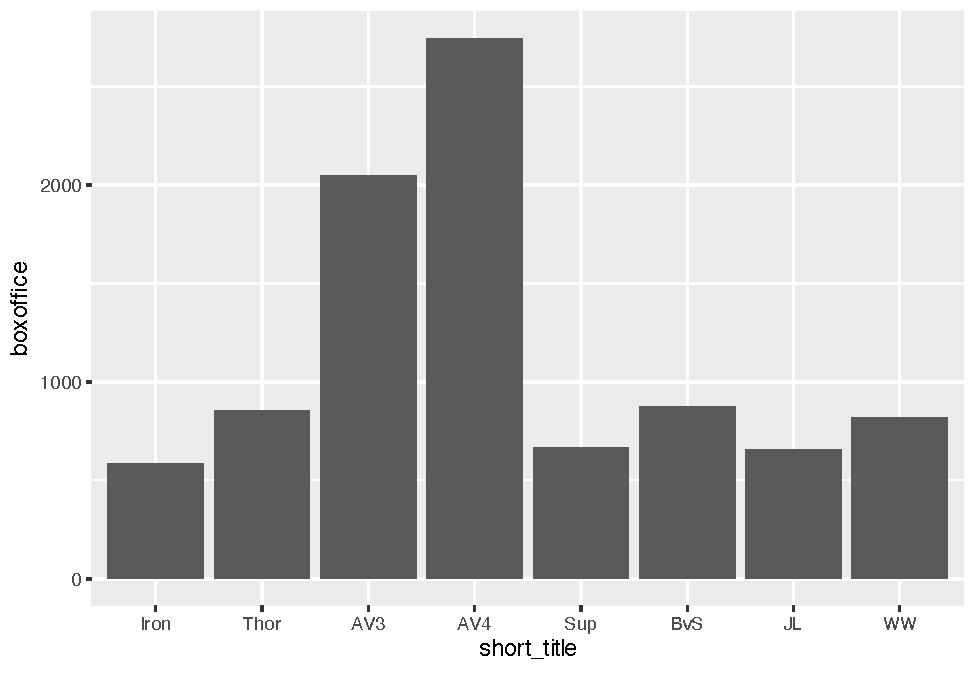
\includegraphics[width=0.65\linewidth]{bookdown_files/figure-latex/unnamed-chunk-114-1}

Next, we want to put the boxoffice revenue above each bar so it easier to interpret. In R terms, we are putting a label above each bar. We want the contents for the labels to come from the boxoffice column. Therefore, we add the geom\_text() command below:

\begin{Shaded}
\begin{Highlighting}[]
\NormalTok{my\_graph }\OtherTok{\textless{}{-}} \FunctionTok{ggplot}\NormalTok{() }\SpecialCharTok{+}
  \FunctionTok{geom\_col}\NormalTok{(}\AttributeTok{data =}\NormalTok{ movie\_data,}
           \AttributeTok{mapping =} \FunctionTok{aes}\NormalTok{(}\AttributeTok{x =}\NormalTok{ short\_title, }
                         \AttributeTok{y =}\NormalTok{ boxoffice)) }\SpecialCharTok{+}
  \FunctionTok{geom\_text}\NormalTok{(}\AttributeTok{data =}\NormalTok{ movie\_data, }
           \AttributeTok{mapping =} \FunctionTok{aes}\NormalTok{(}\AttributeTok{x =}\NormalTok{ short\_title, }
                         \AttributeTok{y =}\NormalTok{ boxoffice, }
                         \AttributeTok{label =}\NormalTok{ boxoffice))}
\FunctionTok{print}\NormalTok{(my\_graph)}
\end{Highlighting}
\end{Shaded}

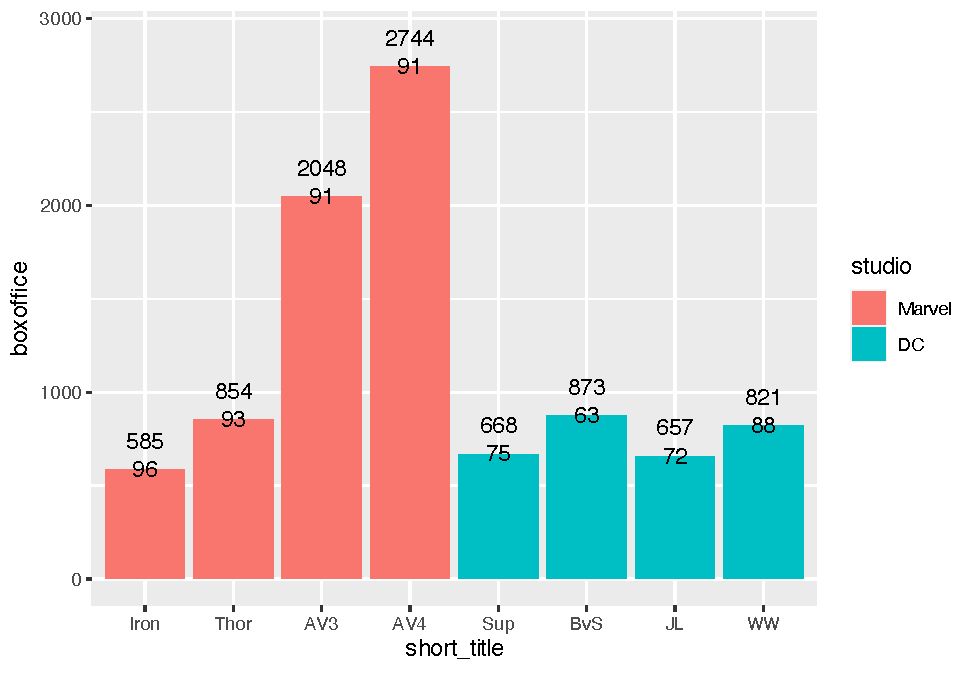
\includegraphics[width=0.65\linewidth]{bookdown_files/figure-latex/unnamed-chunk-115-1}

Unfortunately, when we position the text at the exact height of each column it overlaps with the column making it difficult to read. We fix this on the next page using nudge\_y.

We can nudge each label higher on the y-axis using the \emph{nudge\_y} command. In the above code, we nudge it up 150 units. Since nudge\_y uses the values on the y-axis we are nudging the labels up by 150 million on the y-axis.

\begin{Shaded}
\begin{Highlighting}[]
\NormalTok{my\_graph }\OtherTok{\textless{}{-}} \FunctionTok{ggplot}\NormalTok{() }\SpecialCharTok{+}
  \FunctionTok{geom\_col}\NormalTok{(}\AttributeTok{data =}\NormalTok{ movie\_data,}
           \AttributeTok{mapping =} \FunctionTok{aes}\NormalTok{(}\AttributeTok{x =}\NormalTok{ short\_title, }
                         \AttributeTok{y =}\NormalTok{ boxoffice)) }\SpecialCharTok{+}
  \FunctionTok{geom\_text}\NormalTok{(}\AttributeTok{data =}\NormalTok{ movie\_data, }
           \AttributeTok{mapping =} \FunctionTok{aes}\NormalTok{(}\AttributeTok{x =}\NormalTok{ short\_title, }
                         \AttributeTok{y =}\NormalTok{ boxoffice, }
                         \AttributeTok{label =}\NormalTok{ boxoffice),}
           \AttributeTok{nudge\_y =} \DecValTok{150}\NormalTok{)}

\FunctionTok{print}\NormalTok{(my\_graph)}
\end{Highlighting}
\end{Shaded}

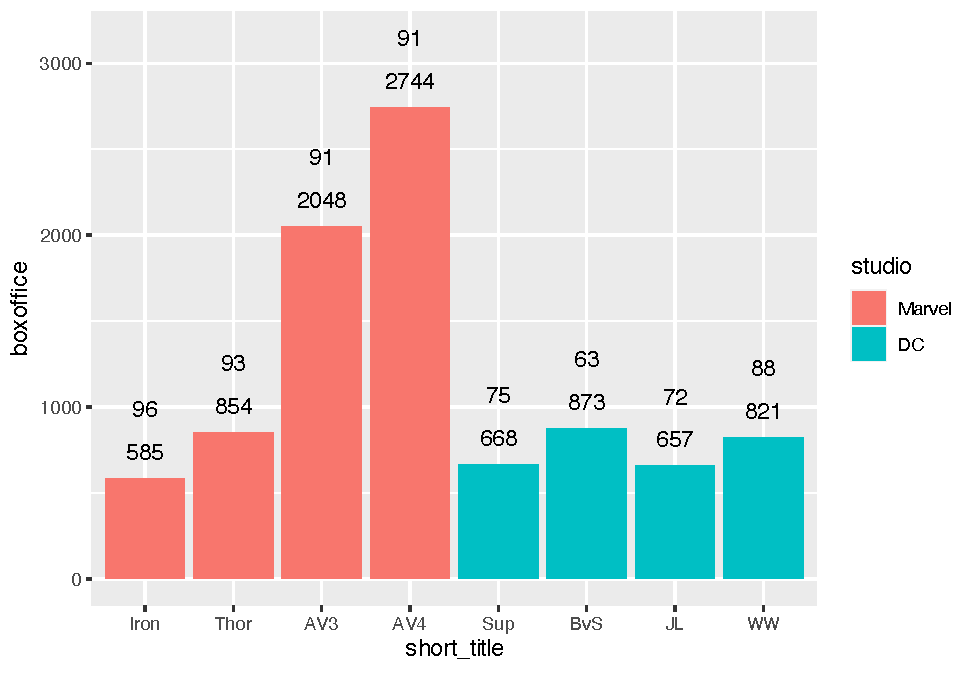
\includegraphics[width=0.65\linewidth]{bookdown_files/figure-latex/unnamed-chunk-116-1}

\section{Graphing efficiently}\label{graphing-efficiently}

You may have noticed that creating the graphs the way we did above required repeating the data and mapping assignments within each command (e.g., geom\_text, geom\_col). Fortunately, we can use a shortcut and specify the data and mapping only once in the ggplot() command. Once we do that, the contents of the mapping argument are invisibly copied into each subsequent command (e.g., geom\_col, geom\_text). In this way, we only have to specify the data and the mapping once.

Examine the code below and compare it to the code above. Notice how in the geom\_col() command we don't have anything specified -- the data and mapping from the ggplot command are used. Likewise, notice how in the geom\_text() command we only specify the arguments we need that are different from those in the ggplot command. In this case, that means simply adding the nudge\_y = 150 to the geom\_text command.

\begin{Shaded}
\begin{Highlighting}[]
\NormalTok{my\_graph }\OtherTok{\textless{}{-}} \FunctionTok{ggplot}\NormalTok{(}\AttributeTok{data =}\NormalTok{ movie\_data,}
           \AttributeTok{mapping =} \FunctionTok{aes}\NormalTok{(}\AttributeTok{x =}\NormalTok{ short\_title,}
                         \AttributeTok{y =}\NormalTok{ boxoffice,}
                         \AttributeTok{label =}\NormalTok{ boxoffice)) }\SpecialCharTok{+}
  \FunctionTok{geom\_col}\NormalTok{() }\SpecialCharTok{+}
  \FunctionTok{geom\_text}\NormalTok{(}\AttributeTok{nudge\_y =} \DecValTok{150}\NormalTok{) }

\FunctionTok{print}\NormalTok{(my\_graph)}
\end{Highlighting}
\end{Shaded}

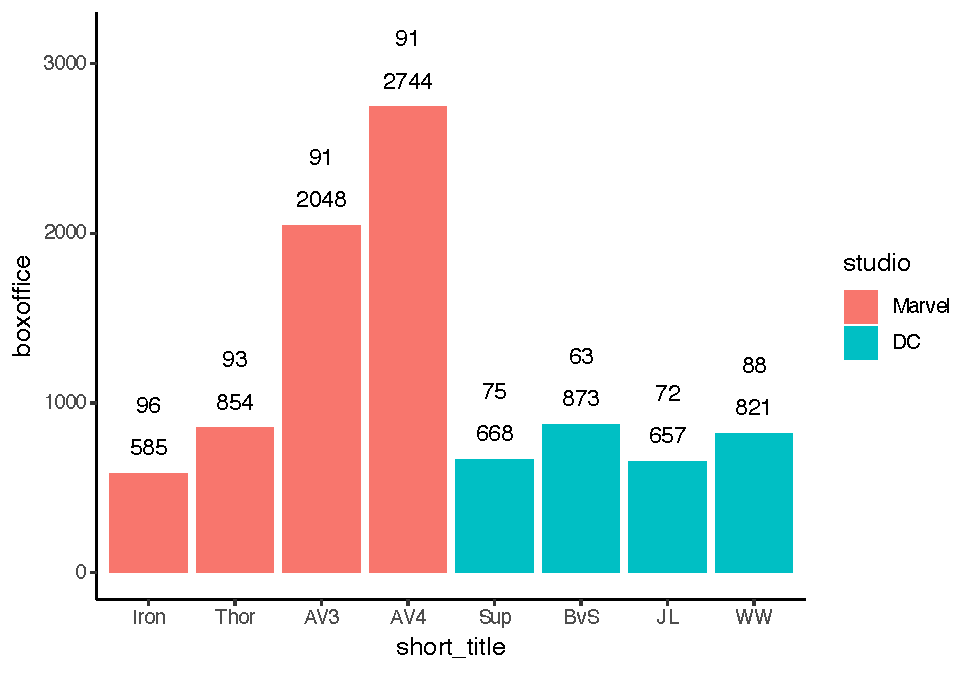
\includegraphics[width=0.65\linewidth]{bookdown_files/figure-latex/unnamed-chunk-117-1}

\section{Aesthetics}\label{aesthetics}

Exactly how does that aesthetic, aes(), command work? What happens when we put the data and mapping in the ggplot() command instead of the specific commands such as geom\_col()? When we put data and the mapping arguments in the ggplot() command we set those attributes for the entire graph. To understand this, you need to know that ggplot uses an internal data set that we will call the ``black box'' data set (i.e., inside the \href{https://en.wikipedia.org/wiki/Black_box}{black box} of ggplot). To create a graph ggplot maps/copies columns from your data set (e.g., movie\_data) to an internal data set. This internal data set is then used to create the graph. Figure \ref{fig:showmap} below illustrates what is happening ``inside the black box'' when you create the graph using the code above.

\begin{figure}
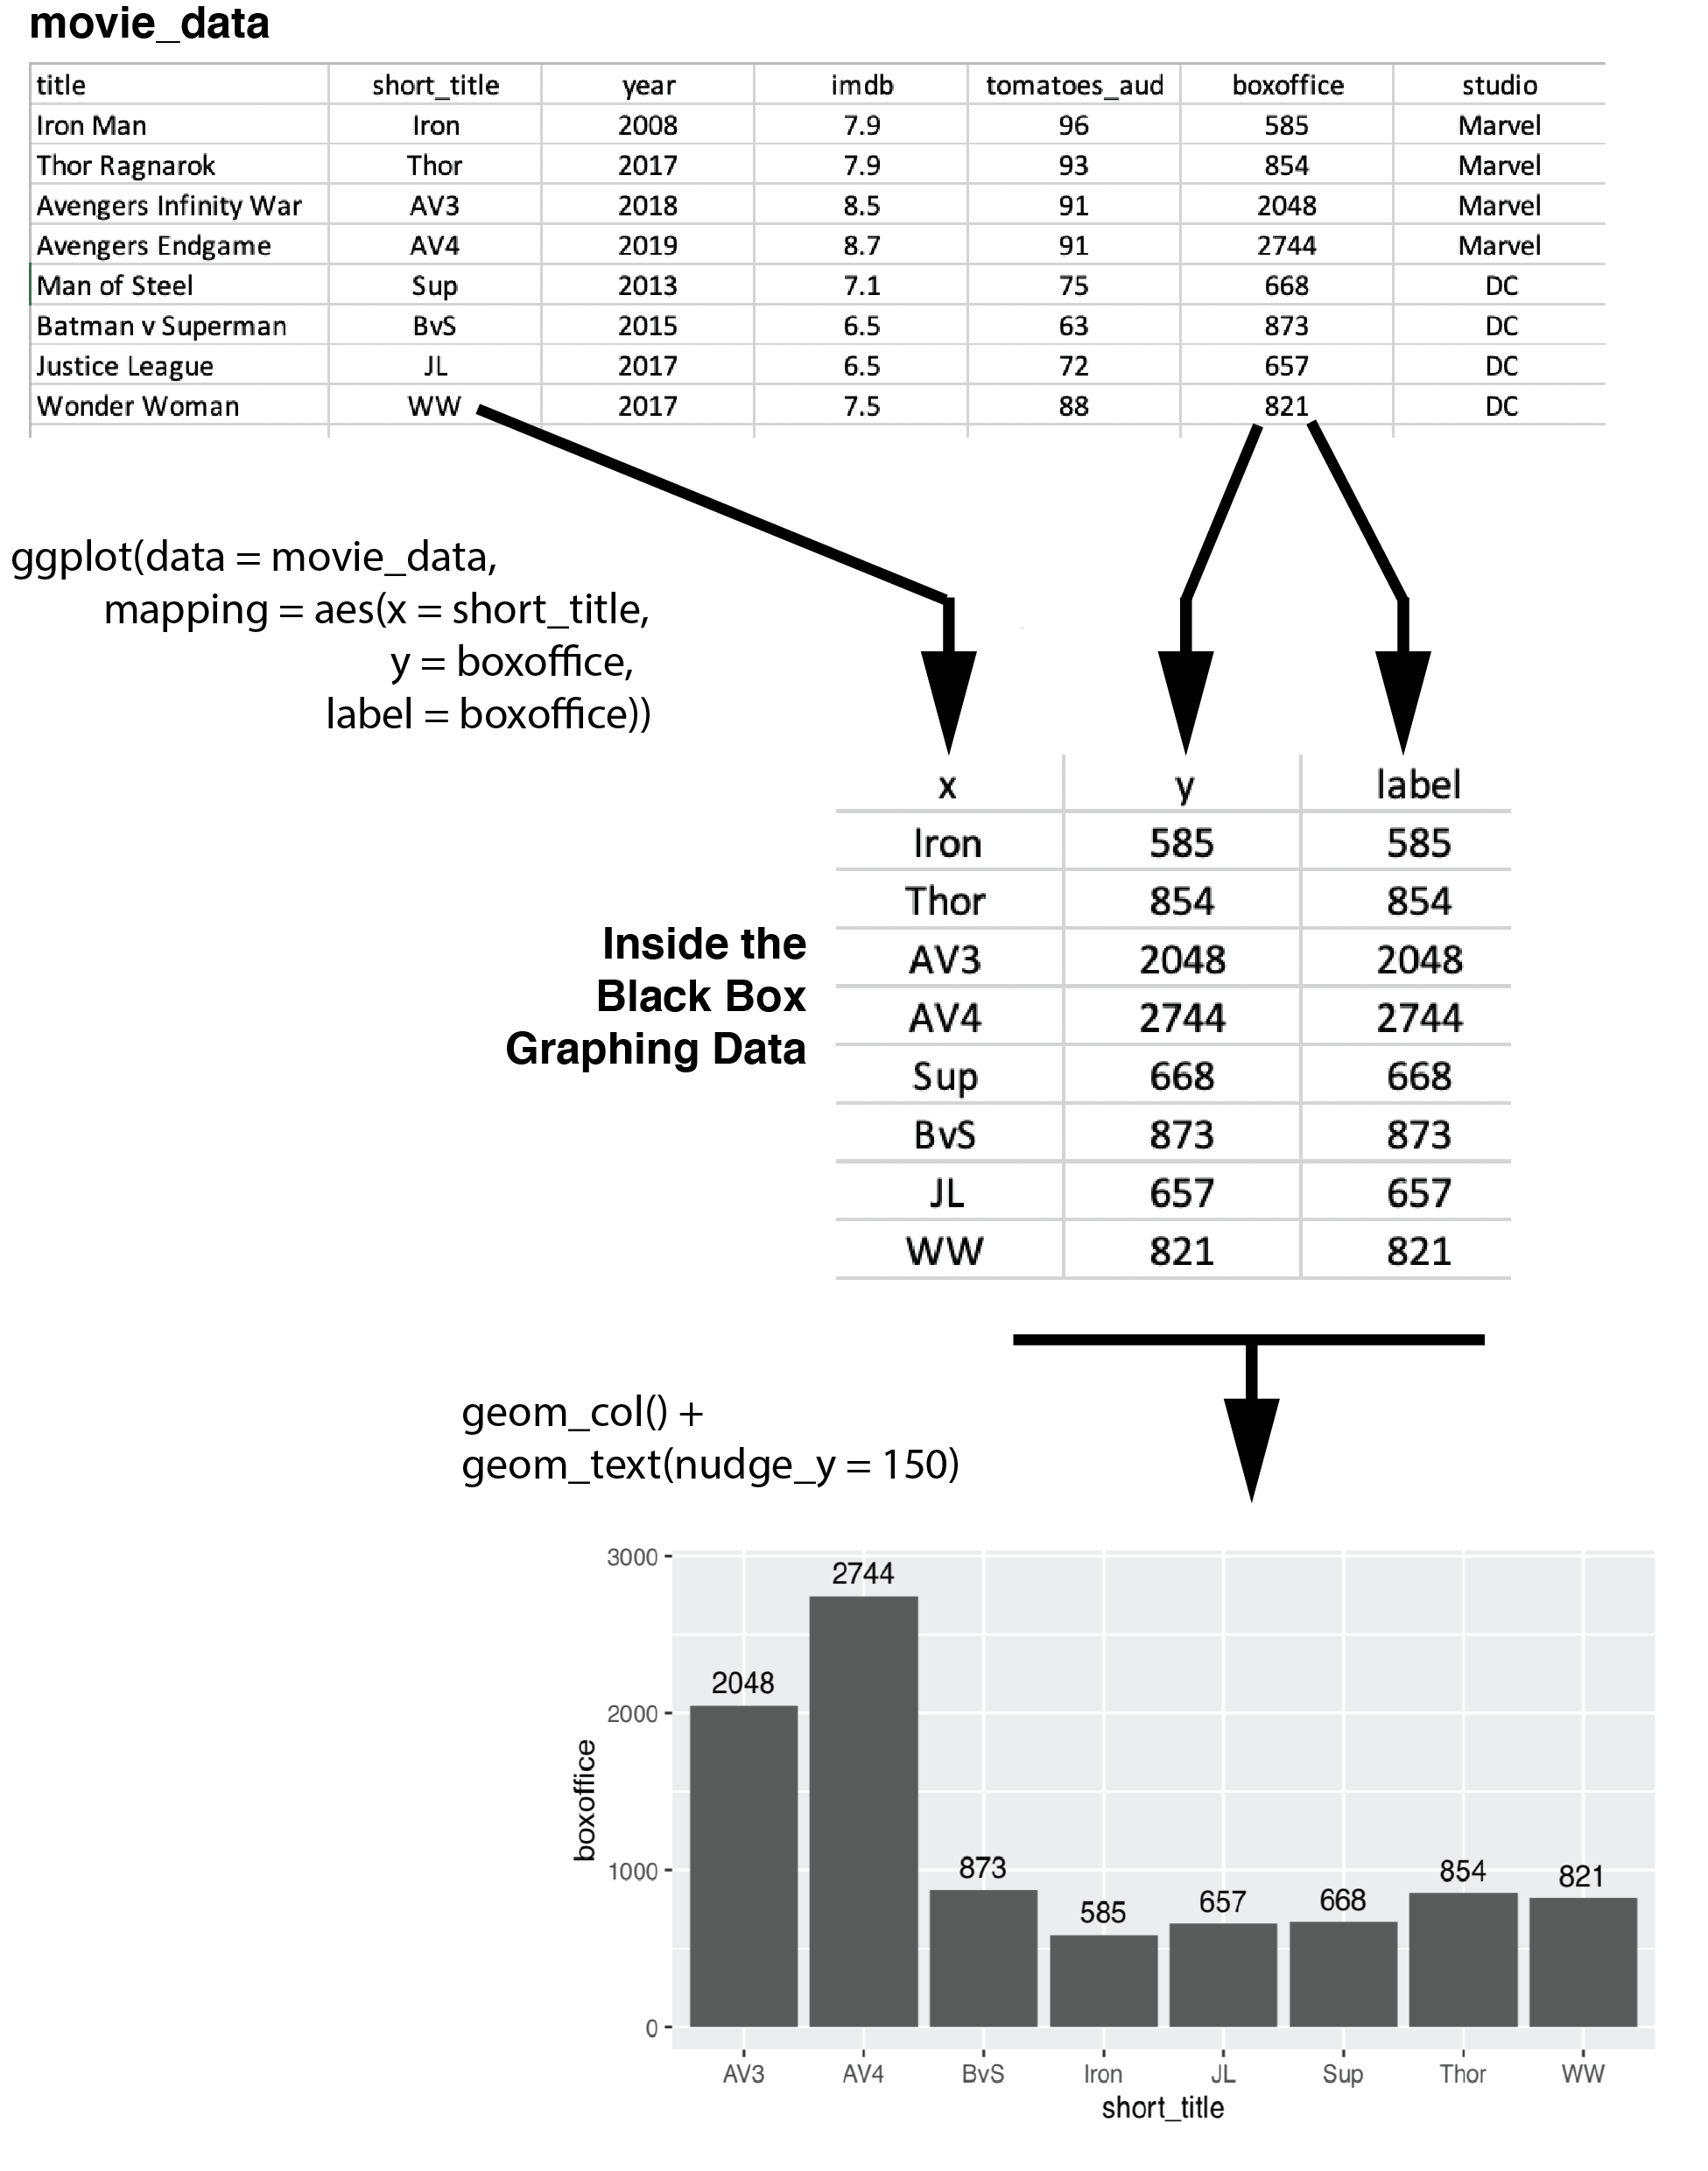
\includegraphics[width=0.7\linewidth]{ch_graphing/images/mapping} \caption{Internal data structure for ggplot}\label{fig:showmap}
\end{figure}

\subsection{Fill color}\label{fill-color}

You might want to influence the color of the bars in the graph such that the bars for Marvel and DC movies have different colors. That's easy to do with the aes() command. We simply tell aes() that the \textbf{fill} color of any object in the graph should be determined by the studio column. Simply adding ``fill = studio'' to the aes() command changes the colors of the bars -- and any other object on the graph for which fill would be relevant. The internal workings are illustrated in Figure \ref{fig:addfill}.

\begin{Shaded}
\begin{Highlighting}[]
\NormalTok{my\_graph }\OtherTok{\textless{}{-}} \FunctionTok{ggplot}\NormalTok{(}\AttributeTok{data =}\NormalTok{ movie\_data,}
           \AttributeTok{mapping =} \FunctionTok{aes}\NormalTok{(}\AttributeTok{x =}\NormalTok{ short\_title,}
                         \AttributeTok{y =}\NormalTok{ boxoffice,}
                         \AttributeTok{label =}\NormalTok{ boxoffice,}
                         \AttributeTok{fill =}\NormalTok{ studio )) }\SpecialCharTok{+}
  \FunctionTok{geom\_col}\NormalTok{() }\SpecialCharTok{+}
  \FunctionTok{geom\_text}\NormalTok{(}\AttributeTok{nudge\_y =} \DecValTok{150}\NormalTok{) }

\FunctionTok{print}\NormalTok{(my\_graph)}
\end{Highlighting}
\end{Shaded}

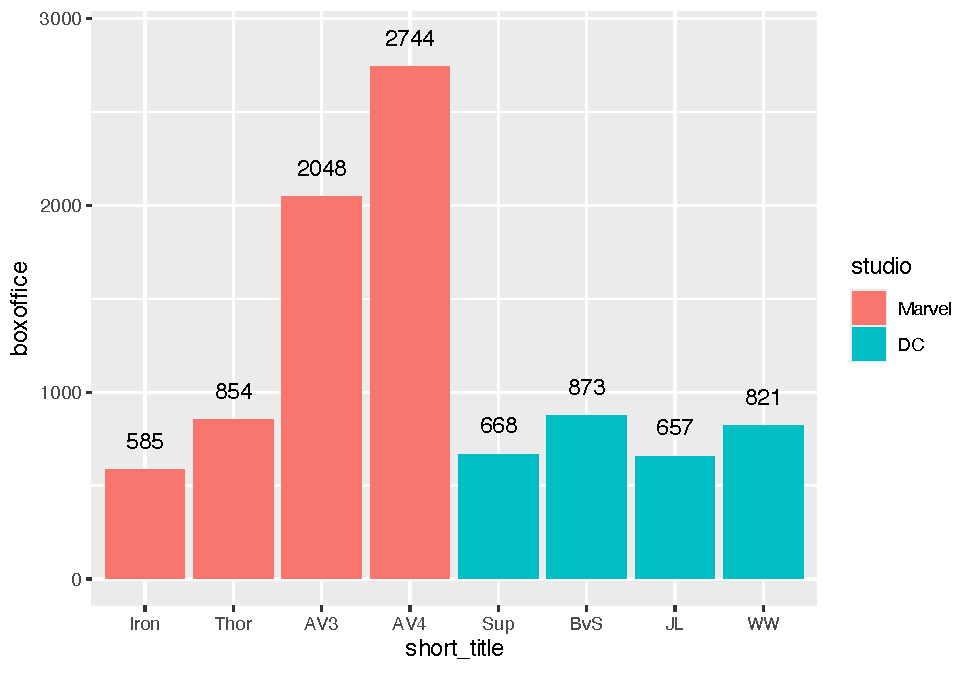
\includegraphics[width=0.65\linewidth]{bookdown_files/figure-latex/unnamed-chunk-118-1}

\begin{figure}
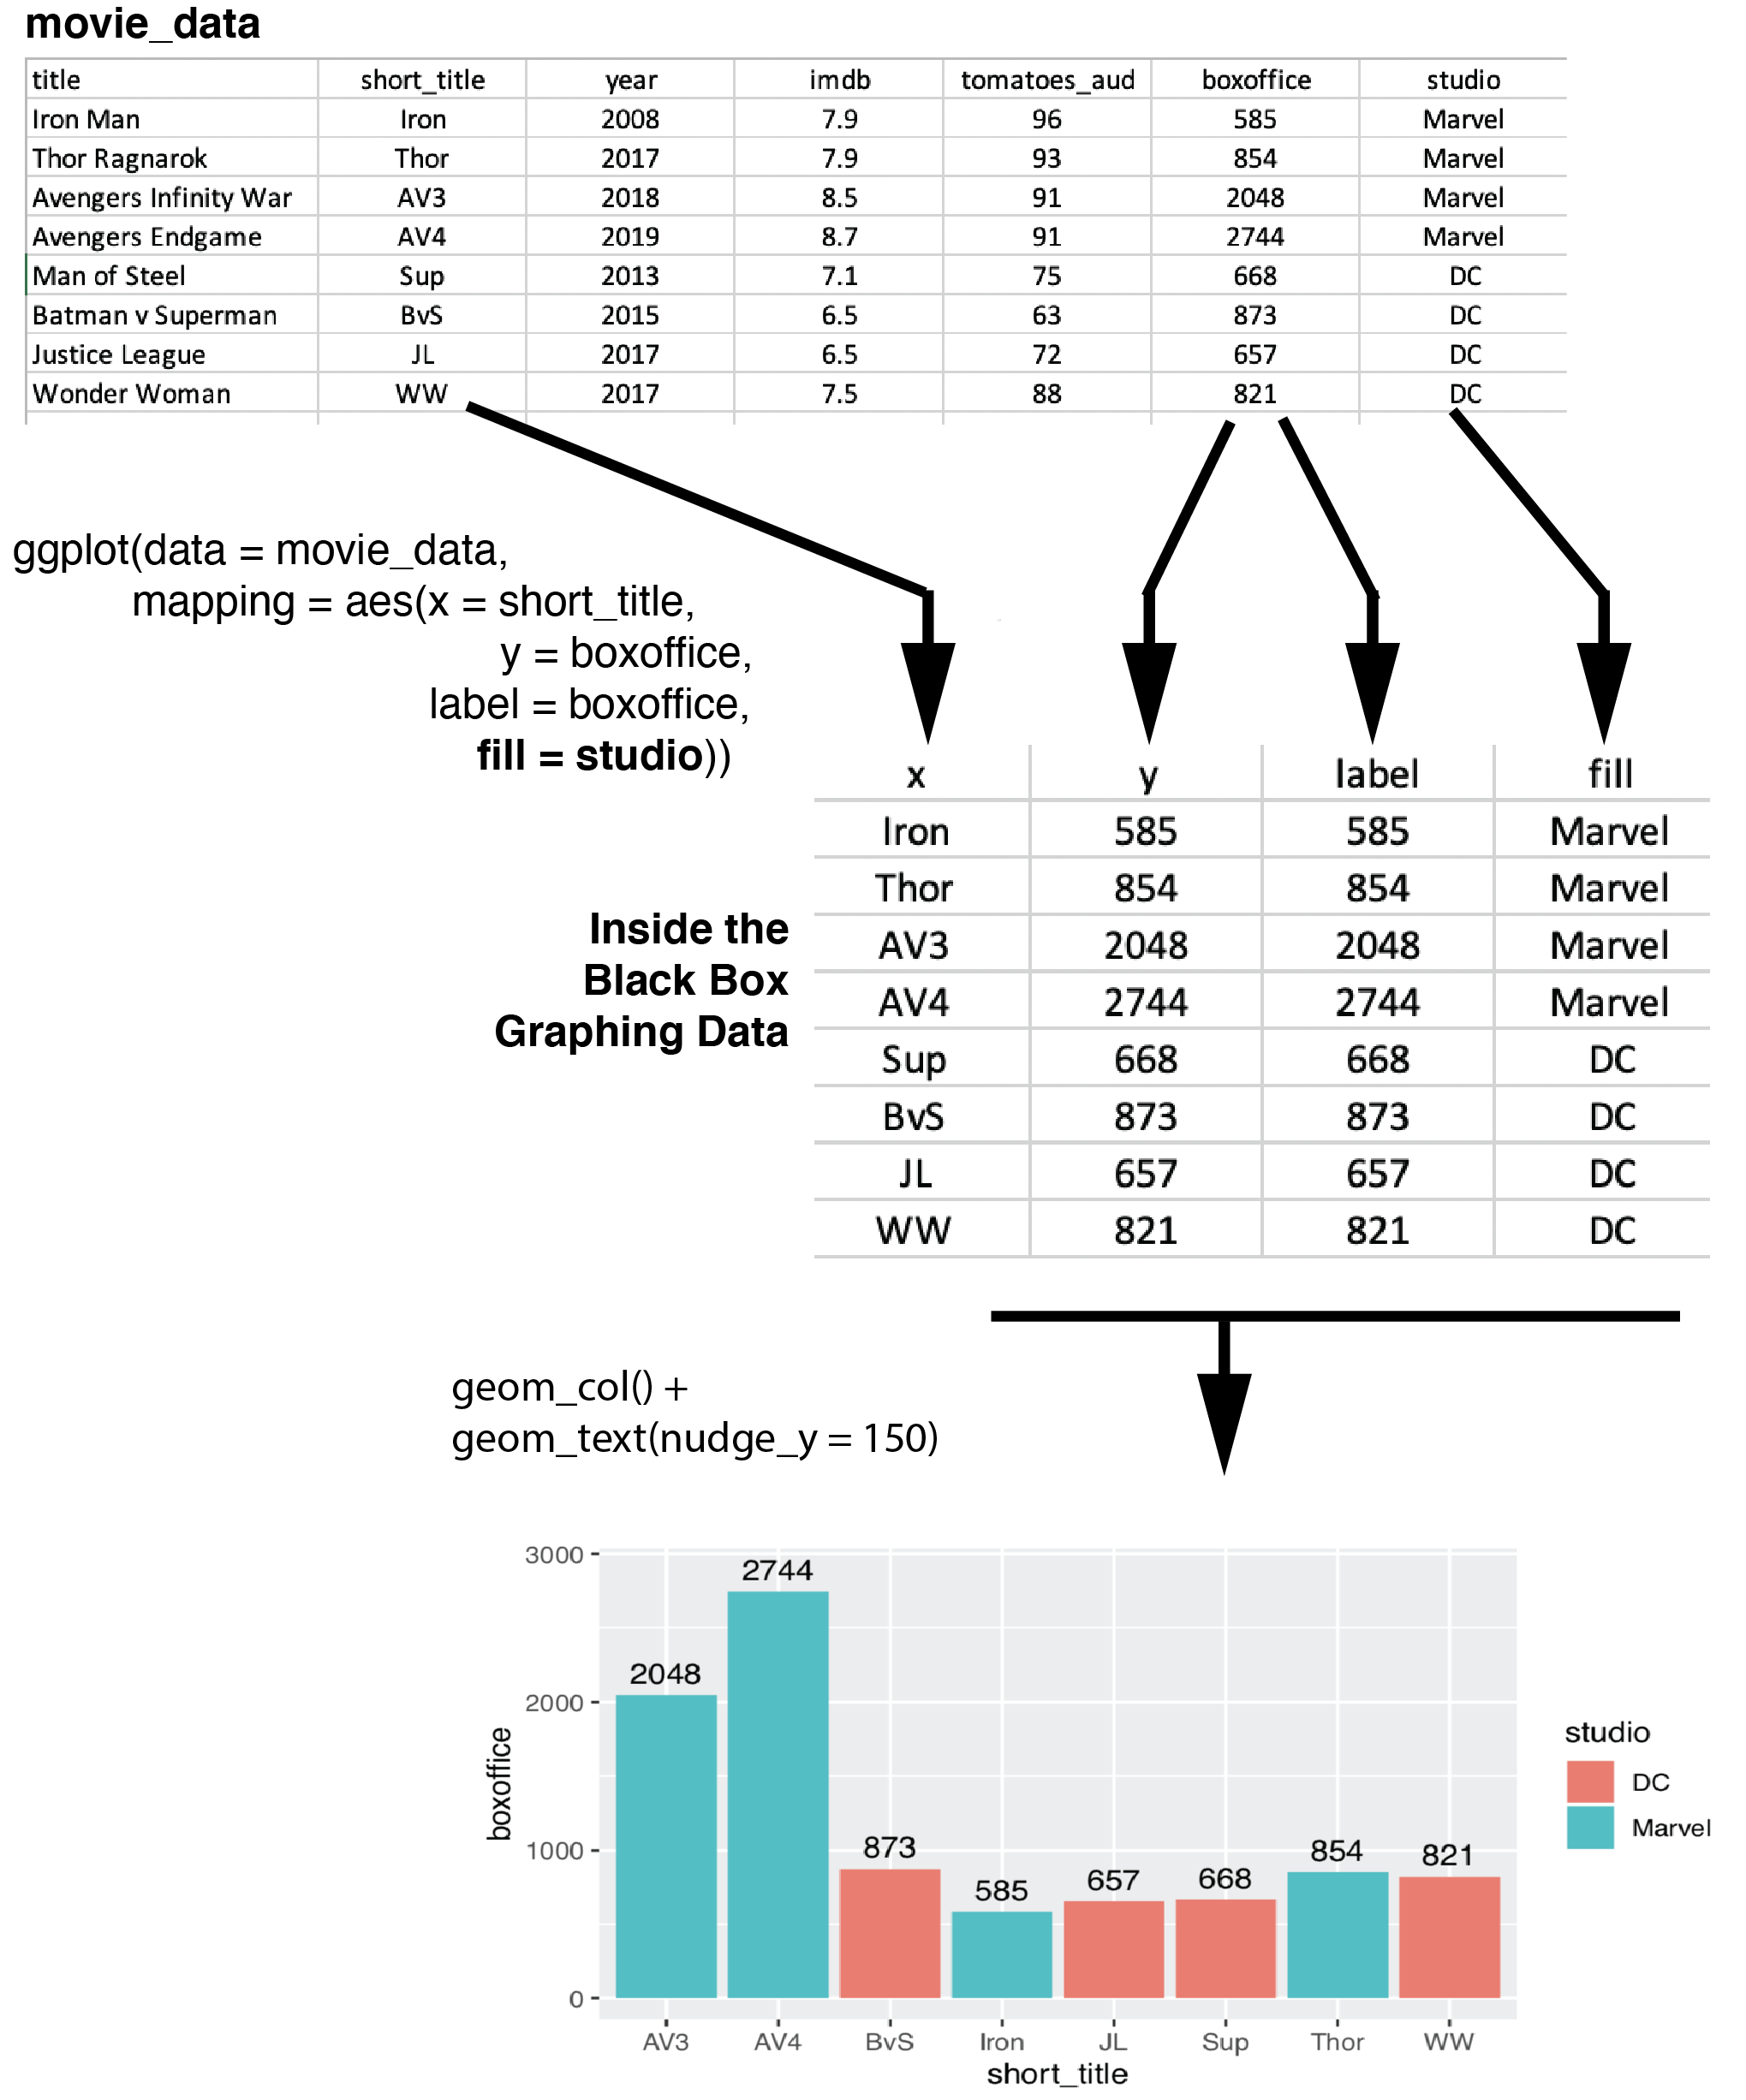
\includegraphics[width=0.7\linewidth]{ch_graphing/images/mapping_fill} \caption{Adding a fill column to the internal data}\label{fig:addfill}
\end{figure}

\subsection{Overriding aes()}\label{overriding-aes}

Just because you specify something in the ggplot() command doesn't mean that you are ``stuck with it'' for all your subsequent commands. Recall how at the start of this exercise we specified the data and the mapping for each geom\_col() and geom\_text() individually. We can still do that.

Now we want to add the Rotten Tomatoes Audience score for each movie above the box office revenue. But if we use geom\_text(), like we did before, it will plot the same boxoffice information because of ``label = boxoffice'' in the aes() specification within ggplot(). We want the new geom\_text() command to plot different text; that is, we want it to use ``label = tomatoes\_aud''.

Fortunately, if we simply put ``mapping = aes(label = tomatoes\_aud)'' within the new geom\_text() command we get the desired information on the graph. The mapping/aes arguments within geom\_text() override the mapping/aes arguments within ggplot(). Or more accurately, the new geom\_text() command creates its own version of the internal data set in which the label column is filled with information from tomatoes\_aud.

\begin{Shaded}
\begin{Highlighting}[]
\NormalTok{my\_graph }\OtherTok{\textless{}{-}} \FunctionTok{ggplot}\NormalTok{(}\AttributeTok{data =}\NormalTok{ movie\_data,}
           \AttributeTok{mapping =} \FunctionTok{aes}\NormalTok{(}\AttributeTok{x =}\NormalTok{ short\_title,}
                         \AttributeTok{y =}\NormalTok{ boxoffice,}
                         \AttributeTok{label =}\NormalTok{ boxoffice, }
                         \AttributeTok{fill =}\NormalTok{ studio)) }\SpecialCharTok{+}
  \FunctionTok{geom\_col}\NormalTok{() }\SpecialCharTok{+}
  \FunctionTok{geom\_text}\NormalTok{(}\AttributeTok{nudge\_y =} \DecValTok{150}\NormalTok{)  }\SpecialCharTok{+}
  \FunctionTok{geom\_text}\NormalTok{(}\AttributeTok{mapping =} \FunctionTok{aes}\NormalTok{(}\AttributeTok{label =}\NormalTok{ tomatoes\_aud)) }
\FunctionTok{print}\NormalTok{(my\_graph)}
\end{Highlighting}
\end{Shaded}

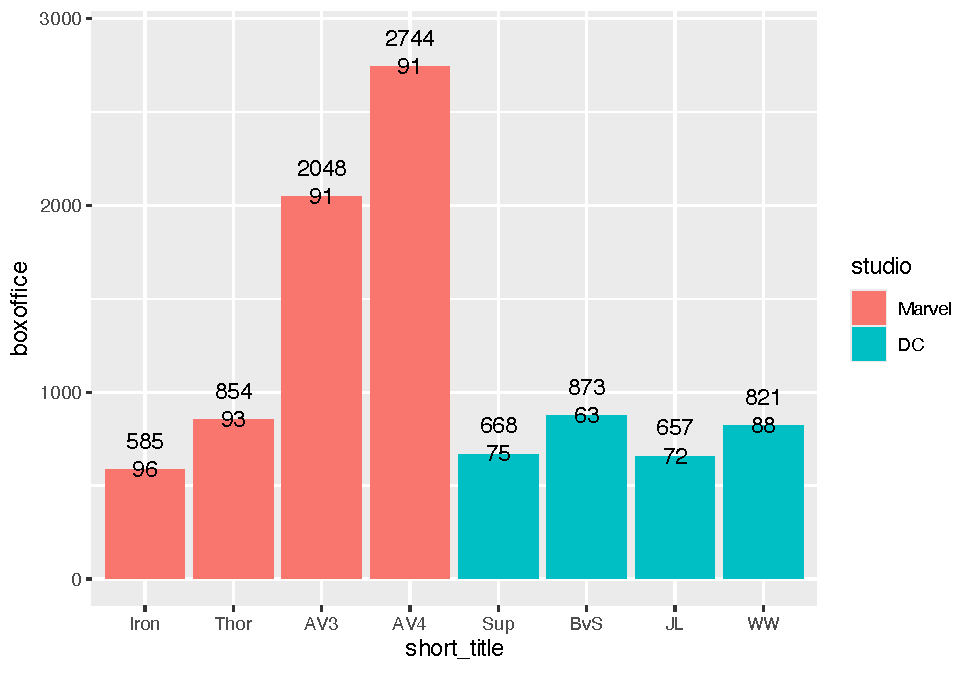
\includegraphics[width=0.65\linewidth]{bookdown_files/figure-latex/unnamed-chunk-119-1}

Notice that we have the same problem as before with the text being difficult to read because it overlaps with the bar. We add ``nudge\_y = 400'' to move the text higher than the boxoffice text/label. Don't forget the units used by nudge\_y are the units on the y-axis.

\begin{Shaded}
\begin{Highlighting}[]
\NormalTok{my\_graph }\OtherTok{\textless{}{-}} \FunctionTok{ggplot}\NormalTok{(}\AttributeTok{data =}\NormalTok{ movie\_data,}
           \AttributeTok{mapping =} \FunctionTok{aes}\NormalTok{(}\AttributeTok{x =}\NormalTok{ short\_title,}
                         \AttributeTok{y =}\NormalTok{ boxoffice,}
                         \AttributeTok{label =}\NormalTok{ boxoffice, }
                         \AttributeTok{fill =}\NormalTok{ studio)) }\SpecialCharTok{+}
  \FunctionTok{geom\_col}\NormalTok{() }\SpecialCharTok{+}
  \FunctionTok{geom\_text}\NormalTok{(}\AttributeTok{nudge\_y =} \DecValTok{150}\NormalTok{)  }\SpecialCharTok{+}
  \FunctionTok{geom\_text}\NormalTok{(}\AttributeTok{mapping =} \FunctionTok{aes}\NormalTok{(}\AttributeTok{label =}\NormalTok{ tomatoes\_aud), }
            \AttributeTok{nudge\_y =} \DecValTok{400}\NormalTok{) }
\FunctionTok{print}\NormalTok{(my\_graph)}
\end{Highlighting}
\end{Shaded}

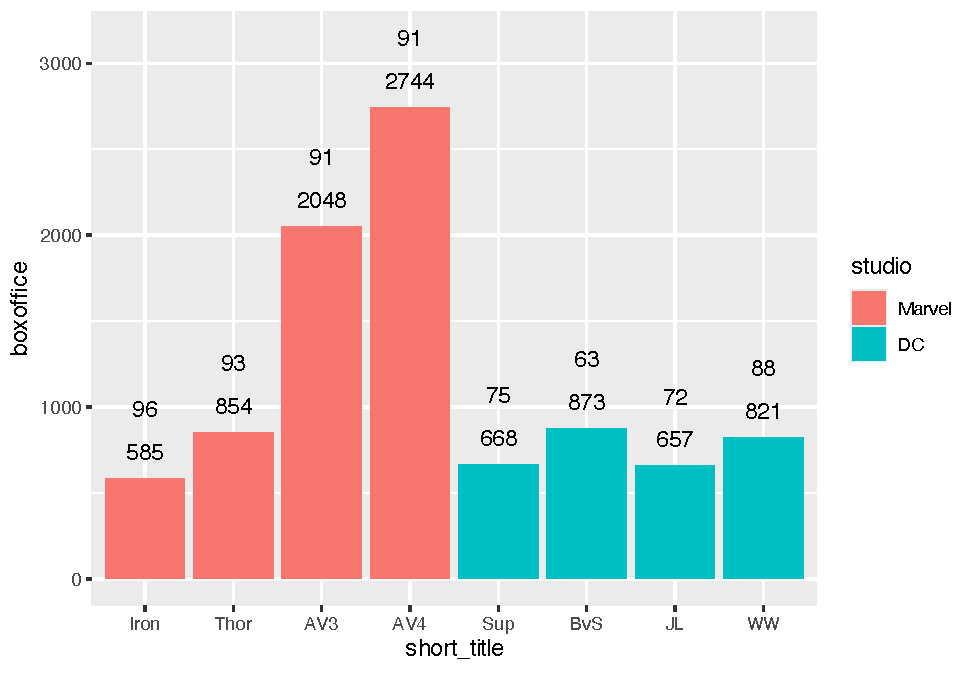
\includegraphics[width=0.65\linewidth]{bookdown_files/figure-latex/unnamed-chunk-120-1}

\newpage

\section{APA style}\label{apa-style}

Use theme\_classic() to make the graph apear in APA style. We use theme\_classic(12) to make the graph APA style with a 12-point font:

\begin{Shaded}
\begin{Highlighting}[]
\NormalTok{my\_graph }\OtherTok{\textless{}{-}} \FunctionTok{ggplot}\NormalTok{(}\AttributeTok{data =}\NormalTok{ movie\_data,}
           \AttributeTok{mapping =} \FunctionTok{aes}\NormalTok{(}\AttributeTok{x =}\NormalTok{ short\_title,}
                         \AttributeTok{y =}\NormalTok{ boxoffice,}
                         \AttributeTok{label =}\NormalTok{ boxoffice, }
                         \AttributeTok{fill =}\NormalTok{ studio)) }\SpecialCharTok{+}
  \FunctionTok{geom\_col}\NormalTok{() }\SpecialCharTok{+}
  \FunctionTok{geom\_text}\NormalTok{(}\AttributeTok{nudge\_y =} \DecValTok{150}\NormalTok{)  }\SpecialCharTok{+}
  \FunctionTok{geom\_text}\NormalTok{(}\AttributeTok{mapping =} \FunctionTok{aes}\NormalTok{(}\AttributeTok{label =}\NormalTok{ tomatoes\_aud), }
            \AttributeTok{nudge\_y =} \DecValTok{400}\NormalTok{) }\SpecialCharTok{+}
  \FunctionTok{theme\_classic}\NormalTok{(}\DecValTok{12}\NormalTok{)}

\FunctionTok{print}\NormalTok{(my\_graph)}
\end{Highlighting}
\end{Shaded}

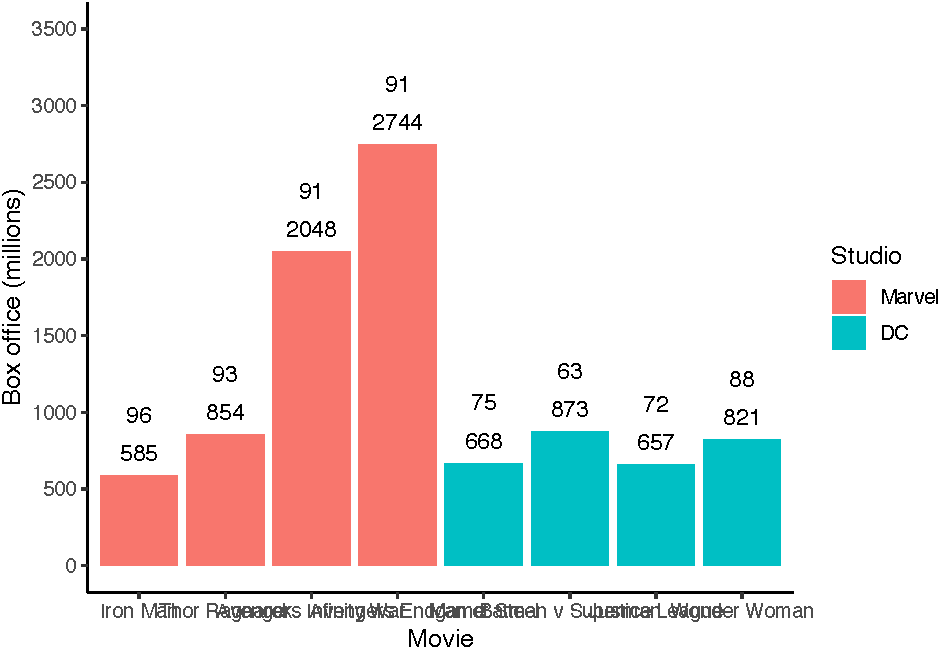
\includegraphics[width=0.65\linewidth]{bookdown_files/figure-latex/unnamed-chunk-121-1}

\section{Axes}\label{axes}

\subsection{Range}\label{range}

We use the coord\_cartesian() command to adjust range of axes. In the code below we use coord\_cartesian() to make the y-axis range from 0 to 3500.

\begin{Shaded}
\begin{Highlighting}[]
\NormalTok{my\_graph }\OtherTok{\textless{}{-}} \FunctionTok{ggplot}\NormalTok{(}\AttributeTok{data =}\NormalTok{ movie\_data,}
           \AttributeTok{mapping =} \FunctionTok{aes}\NormalTok{(}\AttributeTok{x =}\NormalTok{ short\_title,}
                         \AttributeTok{y =}\NormalTok{ boxoffice,}
                         \AttributeTok{label =}\NormalTok{ boxoffice, }
                         \AttributeTok{fill =}\NormalTok{ studio)) }\SpecialCharTok{+}
  \FunctionTok{geom\_col}\NormalTok{() }\SpecialCharTok{+}
  \FunctionTok{geom\_text}\NormalTok{(}\AttributeTok{nudge\_y =} \DecValTok{150}\NormalTok{)  }\SpecialCharTok{+}
  \FunctionTok{geom\_text}\NormalTok{(}\AttributeTok{mapping =} \FunctionTok{aes}\NormalTok{(}\AttributeTok{label =}\NormalTok{ tomatoes\_aud), }
            \AttributeTok{nudge\_y =} \DecValTok{400}\NormalTok{) }\SpecialCharTok{+}
  \FunctionTok{coord\_cartesian}\NormalTok{(}\AttributeTok{ylim =} \FunctionTok{c}\NormalTok{(}\DecValTok{0}\NormalTok{, }\DecValTok{3500}\NormalTok{)) }\SpecialCharTok{+}
  \FunctionTok{theme\_classic}\NormalTok{(}\DecValTok{12}\NormalTok{)}


\FunctionTok{print}\NormalTok{(my\_graph)}
\end{Highlighting}
\end{Shaded}

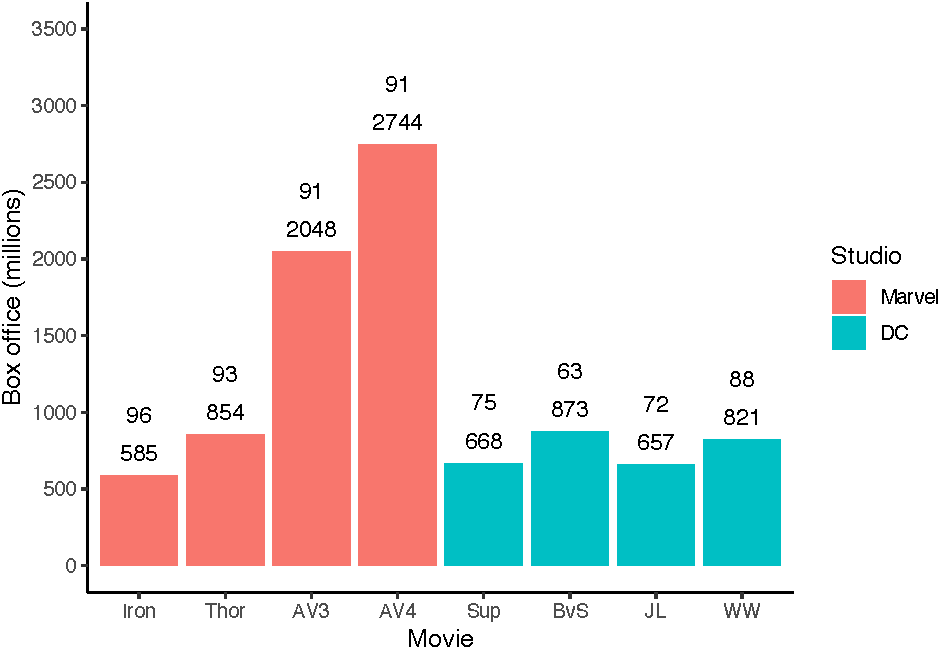
\includegraphics[width=0.65\linewidth]{bookdown_files/figure-latex/unnamed-chunk-122-1}

Note that if you had a continuous variable on the x-axis (we do not in this example), you could set the range of both the x- and y-axes like this:

\begin{Shaded}
\begin{Highlighting}[]
\FunctionTok{coord\_cartesian}\NormalTok{(}\AttributeTok{ylim =} \FunctionTok{c}\NormalTok{(}\DecValTok{0}\NormalTok{, }\DecValTok{3500}\NormalTok{),}
                \AttributeTok{xlim =} \FunctionTok{c}\NormalTok{(}\DecValTok{0}\NormalTok{, }\DecValTok{3500}\NormalTok{))}
\end{Highlighting}
\end{Shaded}

\subsection{Ticks}\label{ticks}

We use the scale\_y\_continuous() command to adjust the ticks on the y-axis. We set the ticks on the y-axis to range from 0 to 3500 in 500 tick increments using the scale\_y\_continuous command below via the breaks argument:

\begin{Shaded}
\begin{Highlighting}[]
\NormalTok{my\_graph }\OtherTok{\textless{}{-}} \FunctionTok{ggplot}\NormalTok{(}\AttributeTok{data =}\NormalTok{ movie\_data,}
           \AttributeTok{mapping =} \FunctionTok{aes}\NormalTok{(}\AttributeTok{x =}\NormalTok{ short\_title,}
                         \AttributeTok{y =}\NormalTok{ boxoffice,}
                         \AttributeTok{label =}\NormalTok{ boxoffice, }
                         \AttributeTok{fill =}\NormalTok{ studio)) }\SpecialCharTok{+}
  \FunctionTok{geom\_col}\NormalTok{() }\SpecialCharTok{+}
  \FunctionTok{geom\_text}\NormalTok{(}\AttributeTok{nudge\_y =} \DecValTok{150}\NormalTok{)  }\SpecialCharTok{+}
  \FunctionTok{geom\_text}\NormalTok{(}\AttributeTok{mapping =} \FunctionTok{aes}\NormalTok{(}\AttributeTok{label =}\NormalTok{ tomatoes\_aud), }
            \AttributeTok{nudge\_y =} \DecValTok{400}\NormalTok{) }\SpecialCharTok{+}
  \FunctionTok{coord\_cartesian}\NormalTok{(}\AttributeTok{ylim =} \FunctionTok{c}\NormalTok{(}\DecValTok{0}\NormalTok{, }\DecValTok{3500}\NormalTok{)) }\SpecialCharTok{+}
  \FunctionTok{scale\_y\_continuous}\NormalTok{(}\AttributeTok{breaks =} \FunctionTok{seq}\NormalTok{(}\DecValTok{0}\NormalTok{, }\DecValTok{3500}\NormalTok{, }\AttributeTok{by =} \DecValTok{500}\NormalTok{)) }\SpecialCharTok{+}
  \FunctionTok{theme\_classic}\NormalTok{(}\DecValTok{12}\NormalTok{)}

\FunctionTok{print}\NormalTok{(my\_graph)}
\end{Highlighting}
\end{Shaded}

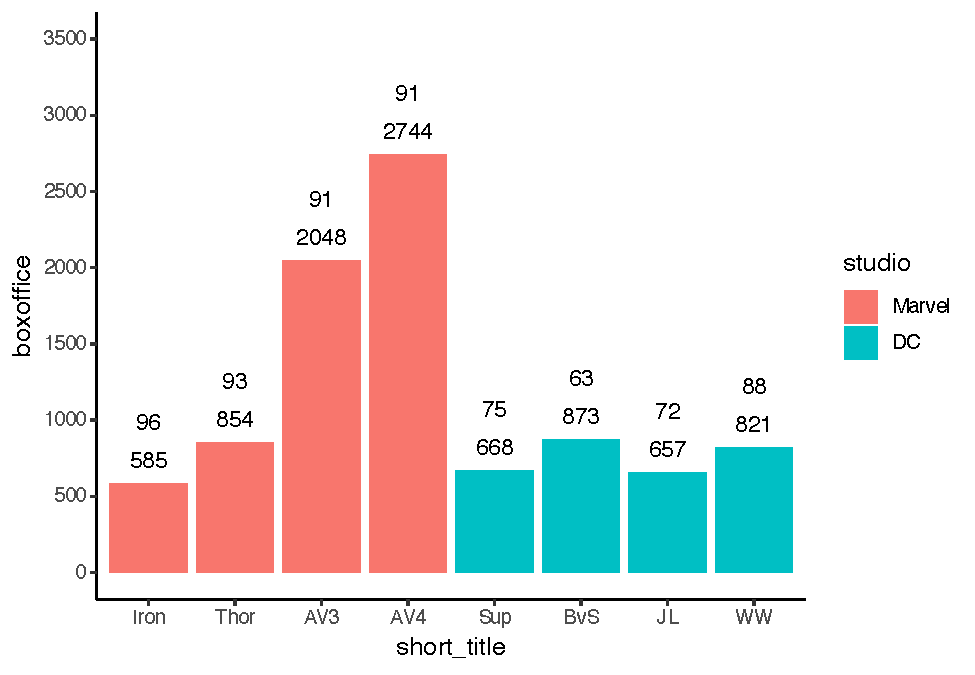
\includegraphics[width=0.65\linewidth]{bookdown_files/figure-latex/unnamed-chunk-124-1}

Note that if you had a continuous variable on the x-axis (we do not in this example), you could set the ticks of the x-axis like the code below using scale\_x\_continuous:

\begin{Shaded}
\begin{Highlighting}[]
\FunctionTok{scale\_x\_continuous}\NormalTok{(}\AttributeTok{breaks =} \FunctionTok{seq}\NormalTok{(}\DecValTok{0}\NormalTok{, }\DecValTok{3500}\NormalTok{, }\AttributeTok{by =} \DecValTok{500}\NormalTok{))}
\end{Highlighting}
\end{Shaded}

\subsection{Labels}\label{labels}

Labels are an extremely important part of any graph. This fact is the focus of the \href{https://xkcd.com/833/}{xkcd} cartoon below:

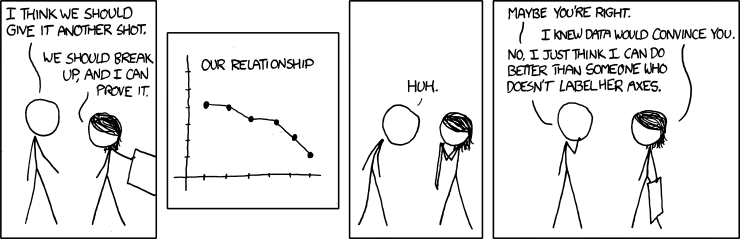
\includegraphics[width=0.8\linewidth]{ch_graphing/images/convincing}

We use the labs() command to set the labels for the x- and y-axes:

\begin{Shaded}
\begin{Highlighting}[]
\NormalTok{my\_graph }\OtherTok{\textless{}{-}} \FunctionTok{ggplot}\NormalTok{(}\AttributeTok{data =}\NormalTok{ movie\_data,}
           \AttributeTok{mapping =} \FunctionTok{aes}\NormalTok{(}\AttributeTok{x =}\NormalTok{ short\_title,}
                         \AttributeTok{y =}\NormalTok{ boxoffice,}
                         \AttributeTok{label =}\NormalTok{ boxoffice, }
                         \AttributeTok{fill =}\NormalTok{ studio)) }\SpecialCharTok{+}
  \FunctionTok{geom\_col}\NormalTok{() }\SpecialCharTok{+}
  \FunctionTok{geom\_text}\NormalTok{(}\AttributeTok{nudge\_y =} \DecValTok{150}\NormalTok{)  }\SpecialCharTok{+}
  \FunctionTok{geom\_text}\NormalTok{(}\AttributeTok{mapping =} \FunctionTok{aes}\NormalTok{(}\AttributeTok{label =}\NormalTok{ tomatoes\_aud), }
            \AttributeTok{nudge\_y =} \DecValTok{400}\NormalTok{) }\SpecialCharTok{+}
  \FunctionTok{coord\_cartesian}\NormalTok{(}\AttributeTok{ylim =} \FunctionTok{c}\NormalTok{(}\DecValTok{0}\NormalTok{, }\DecValTok{3500}\NormalTok{)) }\SpecialCharTok{+}
  \FunctionTok{scale\_y\_continuous}\NormalTok{(}\AttributeTok{breaks =} \FunctionTok{seq}\NormalTok{(}\DecValTok{0}\NormalTok{, }\DecValTok{3500}\NormalTok{, }\AttributeTok{by =} \DecValTok{500}\NormalTok{)) }\SpecialCharTok{+}
  \FunctionTok{labs}\NormalTok{(}\AttributeTok{x =} \StringTok{"Movie"}\NormalTok{,}
       \AttributeTok{y =} \StringTok{"Box office (millions)"}\NormalTok{,}
       \AttributeTok{fill =} \StringTok{"Studio"}\NormalTok{) }\SpecialCharTok{+}
  \FunctionTok{theme\_classic}\NormalTok{(}\DecValTok{12}\NormalTok{)}

\FunctionTok{print}\NormalTok{(my\_graph)}
\end{Highlighting}
\end{Shaded}

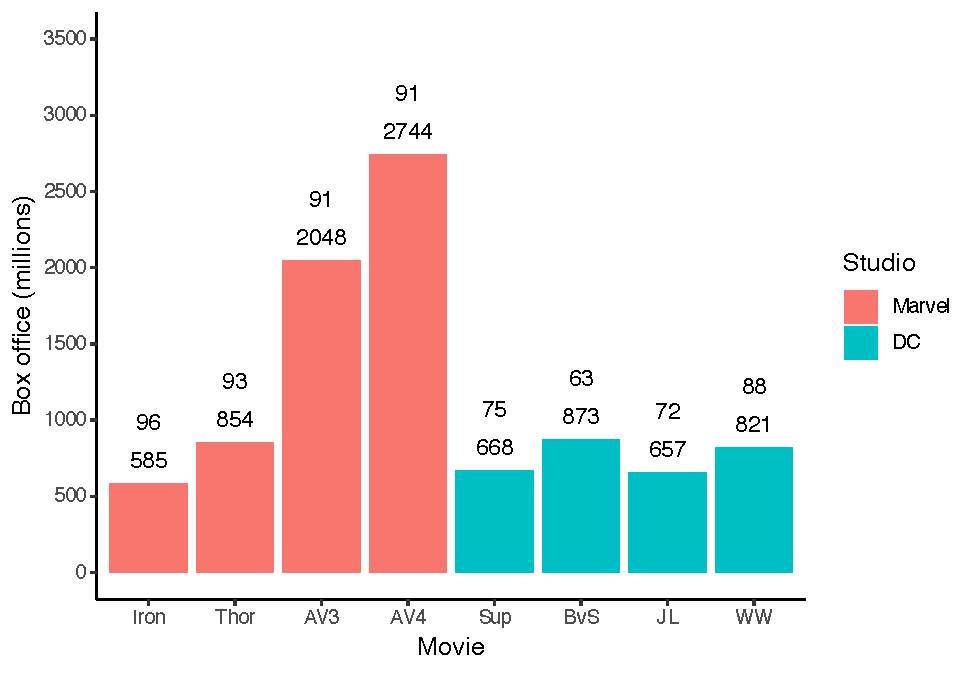
\includegraphics[width=0.65\linewidth]{bookdown_files/figure-latex/unnamed-chunk-127-1}

\section{Axis values}\label{axis-values}

\subsection{Text}\label{text}

What if we want to use the full movie title rather than the short version on the x-axis of the graph? That is, you want to change the values along the x-axis. Two methods are presented below.

\subsubsection{Method 1: Recoding axis values}\label{method-1-recoding-axis-values}

Our data file contains a column with the long/full version of the movie names. But many times you won't have the additional/longer labels available in this manner. In this situation, you use the scale\_x\_discrete() command to change the values along the x-axis.

The values along the x-axis come from the short\_title column which is a factor. The levels of that factor correspond to the short titles for the movies (Iron, Thor, etc.). We need to relabel the levels of the short\_title factor to get a graph with full titles. We relabel the levels of the short\_title factor using the scale\_x\_discrete() command. The graph code with scale\_x\_discrete() command is below - notice the problem we have with the labels overlapping though. On the next page, we'll use an easier approach though - since we have an extra column with the full titles.

\begin{Shaded}
\begin{Highlighting}[]
\NormalTok{my\_graph }\OtherTok{\textless{}{-}} \FunctionTok{ggplot}\NormalTok{(}\AttributeTok{data =}\NormalTok{ movie\_data,}
           \AttributeTok{mapping =} \FunctionTok{aes}\NormalTok{(}\AttributeTok{x =}\NormalTok{ short\_title,}
                         \AttributeTok{y =}\NormalTok{ boxoffice,}
                         \AttributeTok{label =}\NormalTok{ boxoffice, }
                         \AttributeTok{fill =}\NormalTok{ studio)) }\SpecialCharTok{+}
  \FunctionTok{geom\_col}\NormalTok{() }\SpecialCharTok{+}
  \FunctionTok{geom\_text}\NormalTok{(}\AttributeTok{nudge\_y =} \DecValTok{150}\NormalTok{)  }\SpecialCharTok{+}
  \FunctionTok{geom\_text}\NormalTok{(}\AttributeTok{mapping =} \FunctionTok{aes}\NormalTok{(}\AttributeTok{label =}\NormalTok{ tomatoes\_aud), }
            \AttributeTok{nudge\_y =} \DecValTok{400}\NormalTok{) }\SpecialCharTok{+}
  \FunctionTok{coord\_cartesian}\NormalTok{(}\AttributeTok{ylim =} \FunctionTok{c}\NormalTok{(}\DecValTok{0}\NormalTok{, }\DecValTok{3500}\NormalTok{)) }\SpecialCharTok{+}
  \FunctionTok{scale\_y\_continuous}\NormalTok{(}\AttributeTok{breaks =} \FunctionTok{seq}\NormalTok{(}\DecValTok{0}\NormalTok{, }\DecValTok{3500}\NormalTok{, }\AttributeTok{by =} \DecValTok{500}\NormalTok{)) }\SpecialCharTok{+}
  \FunctionTok{scale\_x\_discrete}\NormalTok{(}\AttributeTok{labels=}\FunctionTok{c}\NormalTok{(}\StringTok{"Iron"} \OtherTok{=} \StringTok{"Iron Man"}\NormalTok{, }
                            \StringTok{"Thor"} \OtherTok{=} \StringTok{"Thor Ragnarkok"}\NormalTok{,}
                            \StringTok{"AV3"} \OtherTok{=} \StringTok{"Avengers Infinity War"}\NormalTok{,}
                            \StringTok{"AV4"} \OtherTok{=} \StringTok{"Avengers Endgame"}\NormalTok{,}
                            \StringTok{"Sup"} \OtherTok{=} \StringTok{"Man of Steel"}\NormalTok{,}
                            \StringTok{"BvS"} \OtherTok{=} \StringTok{"Batman v Superman"}\NormalTok{,}
                            \StringTok{"JL"} \OtherTok{=} \StringTok{"Justice League"}\NormalTok{,}
                            \StringTok{"WW"} \OtherTok{=} \StringTok{"Wonder Woman"}\NormalTok{)) }\SpecialCharTok{+}
  \FunctionTok{labs}\NormalTok{(}\AttributeTok{x =} \StringTok{"Movie"}\NormalTok{,}
       \AttributeTok{y =} \StringTok{"Box office (millions)"}\NormalTok{,}
       \AttributeTok{fill =} \StringTok{"Studio"}\NormalTok{) }\SpecialCharTok{+}
  \FunctionTok{theme\_classic}\NormalTok{(}\DecValTok{12}\NormalTok{)}
  

\FunctionTok{print}\NormalTok{(my\_graph)}
\end{Highlighting}
\end{Shaded}

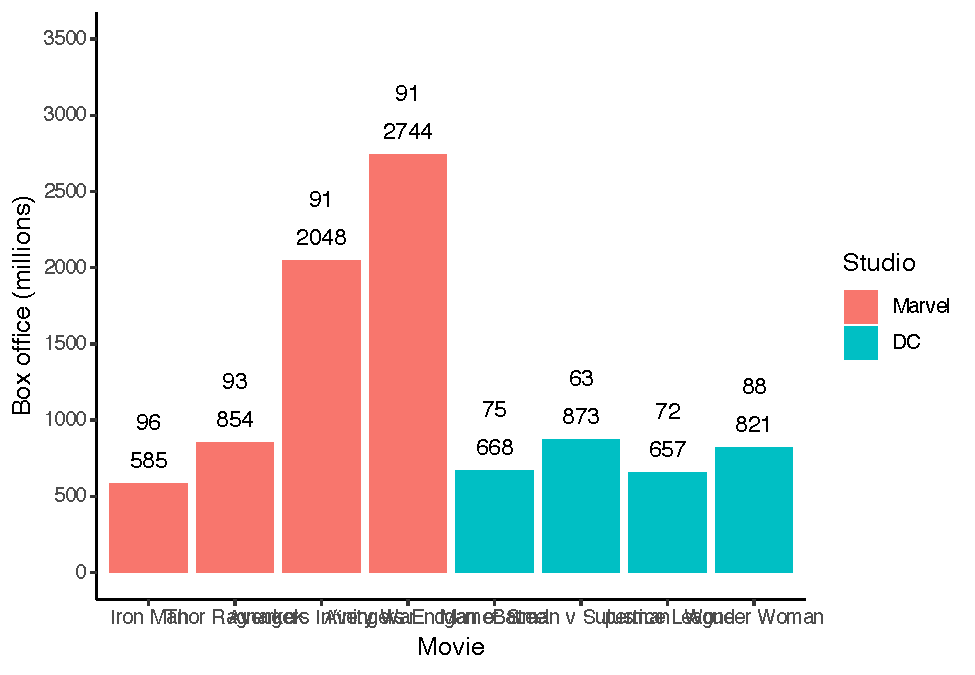
\includegraphics[width=0.65\linewidth]{bookdown_files/figure-latex/unnamed-chunk-128-1}

\subsubsection{Method 2: Longer label columns}\label{method-2-longer-label-columns}

With our movie data we don't need to use scale\_x\_discrete() because we have a column in the data with the full titles. Consequently, to use full length titles we just have to change the \emph{mapping} for x from short\_title to title. Notice that we still have the problem with overlapping labels on the x-axis!

\begin{Shaded}
\begin{Highlighting}[]
\NormalTok{my\_graph }\OtherTok{\textless{}{-}} \FunctionTok{ggplot}\NormalTok{(}\AttributeTok{data =}\NormalTok{ movie\_data,}
           \AttributeTok{mapping =} \FunctionTok{aes}\NormalTok{(}\AttributeTok{x =}\NormalTok{ title,}
                         \AttributeTok{y =}\NormalTok{ boxoffice,}
                         \AttributeTok{label =}\NormalTok{ boxoffice, }
                         \AttributeTok{fill =}\NormalTok{ studio)) }\SpecialCharTok{+}
  \FunctionTok{geom\_col}\NormalTok{() }\SpecialCharTok{+}
  \FunctionTok{geom\_text}\NormalTok{(}\AttributeTok{nudge\_y =} \DecValTok{150}\NormalTok{)  }\SpecialCharTok{+}
  \FunctionTok{geom\_text}\NormalTok{(}\AttributeTok{mapping =} \FunctionTok{aes}\NormalTok{(}\AttributeTok{label =}\NormalTok{ tomatoes\_aud), }
            \AttributeTok{nudge\_y =} \DecValTok{400}\NormalTok{) }\SpecialCharTok{+}
  \FunctionTok{coord\_cartesian}\NormalTok{(}\AttributeTok{ylim =} \FunctionTok{c}\NormalTok{(}\DecValTok{0}\NormalTok{, }\DecValTok{3500}\NormalTok{)) }\SpecialCharTok{+}
  \FunctionTok{scale\_y\_continuous}\NormalTok{(}\AttributeTok{breaks =} \FunctionTok{seq}\NormalTok{(}\DecValTok{0}\NormalTok{, }\DecValTok{3500}\NormalTok{, }\AttributeTok{by =} \DecValTok{500}\NormalTok{)) }\SpecialCharTok{+}
  \FunctionTok{labs}\NormalTok{(}\AttributeTok{x =} \StringTok{"Movie"}\NormalTok{,}
       \AttributeTok{y =} \StringTok{"Box office (millions)"}\NormalTok{,}
       \AttributeTok{fill =} \StringTok{"Studio"}\NormalTok{) }\SpecialCharTok{+}
  \FunctionTok{theme\_classic}\NormalTok{(}\DecValTok{12}\NormalTok{)}
  

\FunctionTok{print}\NormalTok{(my\_graph)}
\end{Highlighting}
\end{Shaded}

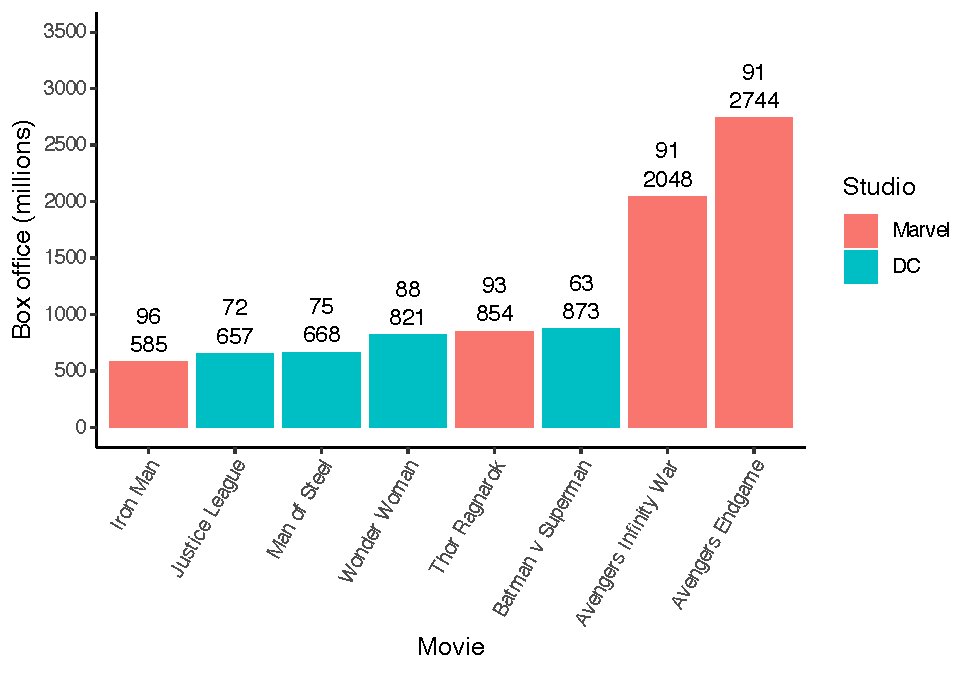
\includegraphics[width=0.65\linewidth]{bookdown_files/figure-latex/unnamed-chunk-129-1}

\subsection{Angle}\label{angle}

Use theme() to adjust the angle of x-axis labels. Notice, however, that the longer titles are vertically centered on each point on the x-axis. In the next section we fix this problem.

\textbf{Important}: The theme command must come after the theme\_classic command. Otherwise, theme\_classic will undo the work done by the theme\_command if it appears after the theme command.

\begin{Shaded}
\begin{Highlighting}[]
\NormalTok{my\_graph }\OtherTok{\textless{}{-}} \FunctionTok{ggplot}\NormalTok{(}\AttributeTok{data =}\NormalTok{ movie\_data,}
           \AttributeTok{mapping =} \FunctionTok{aes}\NormalTok{(}\AttributeTok{x =}\NormalTok{ title,}
                         \AttributeTok{y =}\NormalTok{ boxoffice,}
                         \AttributeTok{label =}\NormalTok{ boxoffice, }
                         \AttributeTok{fill =}\NormalTok{ studio)) }\SpecialCharTok{+}
  \FunctionTok{geom\_col}\NormalTok{() }\SpecialCharTok{+}
  \FunctionTok{geom\_text}\NormalTok{(}\AttributeTok{nudge\_y =} \DecValTok{150}\NormalTok{)  }\SpecialCharTok{+}
  \FunctionTok{geom\_text}\NormalTok{(}\AttributeTok{mapping =} \FunctionTok{aes}\NormalTok{(}\AttributeTok{label =}\NormalTok{ tomatoes\_aud), }
            \AttributeTok{nudge\_y =} \DecValTok{400}\NormalTok{) }\SpecialCharTok{+}
  \FunctionTok{coord\_cartesian}\NormalTok{(}\AttributeTok{ylim =} \FunctionTok{c}\NormalTok{(}\DecValTok{0}\NormalTok{, }\DecValTok{3500}\NormalTok{)) }\SpecialCharTok{+}
  \FunctionTok{scale\_y\_continuous}\NormalTok{(}\AttributeTok{breaks =} \FunctionTok{seq}\NormalTok{(}\DecValTok{0}\NormalTok{, }\DecValTok{3500}\NormalTok{, }\AttributeTok{by =} \DecValTok{500}\NormalTok{)) }\SpecialCharTok{+}
  \FunctionTok{labs}\NormalTok{(}\AttributeTok{x =} \StringTok{"Movie"}\NormalTok{,}
       \AttributeTok{y =} \StringTok{"Box office (millions)"}\NormalTok{,}
       \AttributeTok{fill =} \StringTok{"Studio"}\NormalTok{) }\SpecialCharTok{+}
  \FunctionTok{theme\_classic}\NormalTok{(}\DecValTok{12}\NormalTok{) }\SpecialCharTok{+}
  \FunctionTok{theme}\NormalTok{(}\AttributeTok{axis.text.x =} \FunctionTok{element\_text}\NormalTok{(}\AttributeTok{angle =} \DecValTok{60}\NormalTok{))}

\FunctionTok{print}\NormalTok{(my\_graph)}
\end{Highlighting}
\end{Shaded}

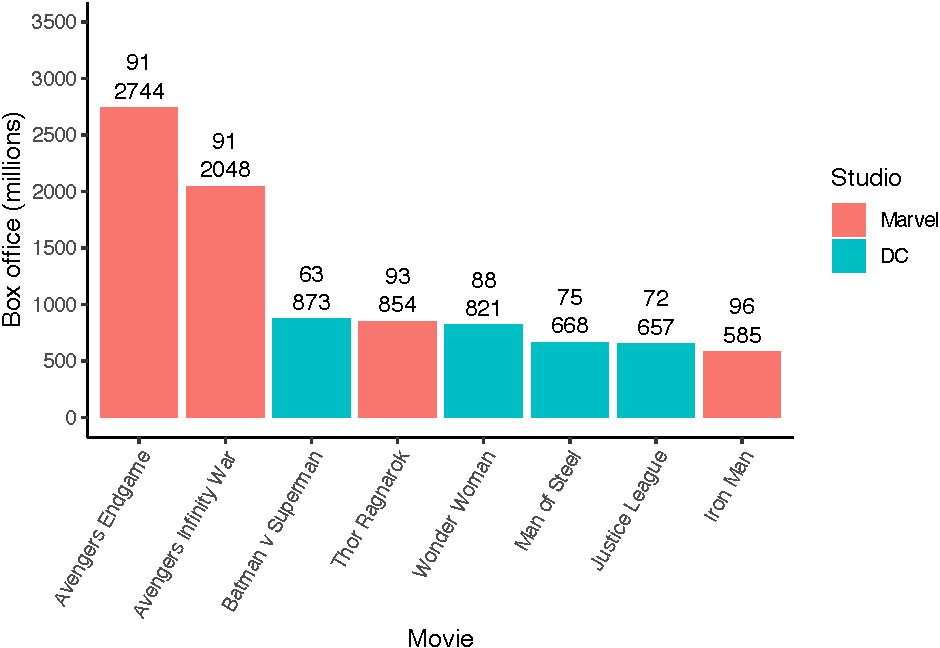
\includegraphics[width=0.65\linewidth]{bookdown_files/figure-latex/unnamed-chunk-130-1}

\subsection{Alignment}\label{alignment}

Use theme() and the hjust argument to adjust the alignment of the x-axis labels. To make the titles look correct on the x-axis we need them at an angle, but we also need them right justified against the x-axis. We do that with the the hjust argument (1 means right justify). See the code below:

\begin{Shaded}
\begin{Highlighting}[]
\NormalTok{my\_graph }\OtherTok{\textless{}{-}} \FunctionTok{ggplot}\NormalTok{(}\AttributeTok{data =}\NormalTok{ movie\_data,}
           \AttributeTok{mapping =} \FunctionTok{aes}\NormalTok{(}\AttributeTok{x =}\NormalTok{ title,}
                         \AttributeTok{y =}\NormalTok{ boxoffice,}
                         \AttributeTok{label =}\NormalTok{ boxoffice, }
                         \AttributeTok{fill =}\NormalTok{ studio)) }\SpecialCharTok{+}
  \FunctionTok{geom\_col}\NormalTok{() }\SpecialCharTok{+}
  \FunctionTok{geom\_text}\NormalTok{(}\AttributeTok{nudge\_y =} \DecValTok{150}\NormalTok{)  }\SpecialCharTok{+}
  \FunctionTok{geom\_text}\NormalTok{(}\AttributeTok{mapping =} \FunctionTok{aes}\NormalTok{(}\AttributeTok{label =}\NormalTok{ tomatoes\_aud), }
            \AttributeTok{nudge\_y =} \DecValTok{400}\NormalTok{) }\SpecialCharTok{+}
  \FunctionTok{coord\_cartesian}\NormalTok{(}\AttributeTok{ylim =} \FunctionTok{c}\NormalTok{(}\DecValTok{0}\NormalTok{, }\DecValTok{3500}\NormalTok{)) }\SpecialCharTok{+}
  \FunctionTok{scale\_y\_continuous}\NormalTok{(}\AttributeTok{breaks =} \FunctionTok{seq}\NormalTok{(}\DecValTok{0}\NormalTok{, }\DecValTok{3500}\NormalTok{, }\AttributeTok{by =} \DecValTok{500}\NormalTok{)) }\SpecialCharTok{+}
  \FunctionTok{labs}\NormalTok{(}\AttributeTok{x =} \StringTok{"Movie"}\NormalTok{,}
       \AttributeTok{y =} \StringTok{"Box office (millions)"}\NormalTok{,}
       \AttributeTok{fill =} \StringTok{"Studio"}\NormalTok{) }\SpecialCharTok{+}
  \FunctionTok{theme\_classic}\NormalTok{(}\DecValTok{12}\NormalTok{) }\SpecialCharTok{+}
  \FunctionTok{theme}\NormalTok{(}\AttributeTok{axis.text.x =} \FunctionTok{element\_text}\NormalTok{(}\AttributeTok{angle =} \DecValTok{60}\NormalTok{, }
                                   \AttributeTok{hjust =} \DecValTok{1}\NormalTok{))  }

\FunctionTok{print}\NormalTok{(my\_graph)}
\end{Highlighting}
\end{Shaded}

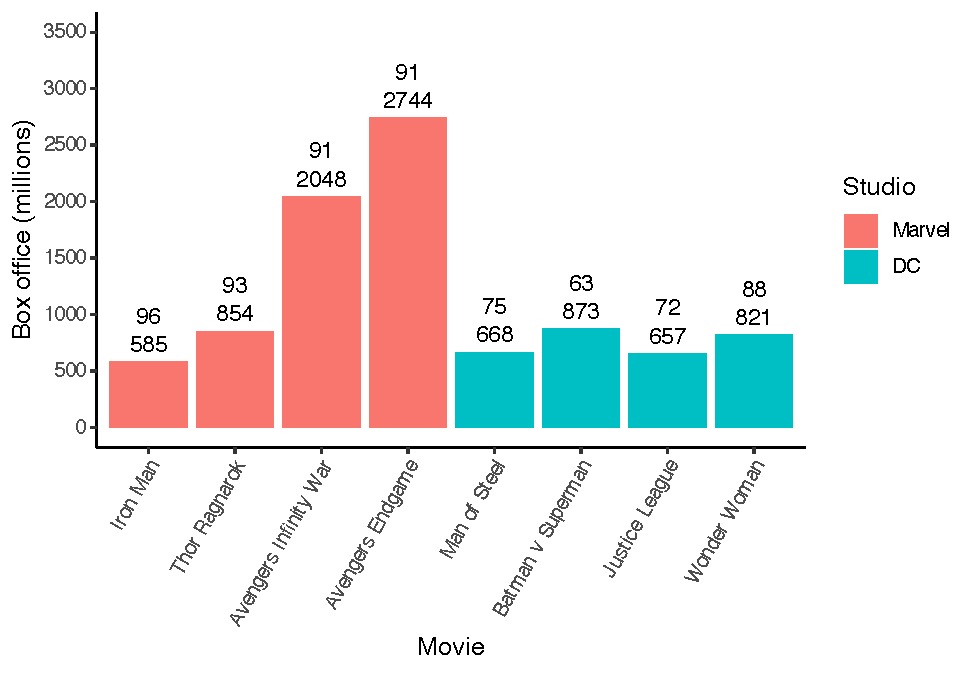
\includegraphics[width=0.65\linewidth]{bookdown_files/figure-latex/unnamed-chunk-131-1}

\subsection{Order}\label{order}

\subsubsection{Increasing order}\label{increasing-order}

We can make the movie bars go left to right in lowest to highest box office receipt order by changing the factor order prior to creating the graph. We do so with the mutate() and fct\_reorder() commands. The default order is ascending values even though we don't specify it.

\begin{Shaded}
\begin{Highlighting}[]
\NormalTok{movie\_data }\OtherTok{\textless{}{-}}\NormalTok{ movie\_data }\SpecialCharTok{\%\textgreater{}\%} 
  \FunctionTok{mutate}\NormalTok{(}\AttributeTok{title =} \FunctionTok{fct\_reorder}\NormalTok{(title,}
\NormalTok{                             boxoffice))}
\end{Highlighting}
\end{Shaded}

\begin{Shaded}
\begin{Highlighting}[]
\NormalTok{my\_graph }\OtherTok{\textless{}{-}} \FunctionTok{ggplot}\NormalTok{(}\AttributeTok{data =}\NormalTok{ movie\_data,}
           \AttributeTok{mapping =} \FunctionTok{aes}\NormalTok{(}\AttributeTok{x =}\NormalTok{ title,}
                         \AttributeTok{y =}\NormalTok{ boxoffice,}
                         \AttributeTok{label =}\NormalTok{ boxoffice, }
                         \AttributeTok{fill =}\NormalTok{ studio)) }\SpecialCharTok{+}
  \FunctionTok{geom\_col}\NormalTok{() }\SpecialCharTok{+}
  \FunctionTok{geom\_text}\NormalTok{(}\AttributeTok{nudge\_y =} \DecValTok{150}\NormalTok{)  }\SpecialCharTok{+}
  \FunctionTok{geom\_text}\NormalTok{(}\AttributeTok{mapping =} \FunctionTok{aes}\NormalTok{(}\AttributeTok{label =}\NormalTok{ tomatoes\_aud), }
            \AttributeTok{nudge\_y =} \DecValTok{400}\NormalTok{) }\SpecialCharTok{+}
  \FunctionTok{coord\_cartesian}\NormalTok{(}\AttributeTok{ylim =} \FunctionTok{c}\NormalTok{(}\DecValTok{0}\NormalTok{, }\DecValTok{3500}\NormalTok{)) }\SpecialCharTok{+}
  \FunctionTok{scale\_y\_continuous}\NormalTok{(}\AttributeTok{breaks =} \FunctionTok{seq}\NormalTok{(}\DecValTok{0}\NormalTok{, }\DecValTok{3500}\NormalTok{, }\AttributeTok{by =} \DecValTok{500}\NormalTok{)) }\SpecialCharTok{+}
  \FunctionTok{labs}\NormalTok{(}\AttributeTok{x =} \StringTok{"Movie"}\NormalTok{,}
       \AttributeTok{y =} \StringTok{"Box office (millions)"}\NormalTok{,}
       \AttributeTok{fill =} \StringTok{"Studio"}\NormalTok{) }\SpecialCharTok{+}
  \FunctionTok{theme\_classic}\NormalTok{(}\DecValTok{12}\NormalTok{) }\SpecialCharTok{+}
  \FunctionTok{theme}\NormalTok{(}\AttributeTok{axis.text.x =} \FunctionTok{element\_text}\NormalTok{(}\AttributeTok{angle =} \DecValTok{60}\NormalTok{, }
                                   \AttributeTok{hjust =} \DecValTok{1}\NormalTok{))  }

\FunctionTok{print}\NormalTok{(my\_graph)}
\end{Highlighting}
\end{Shaded}

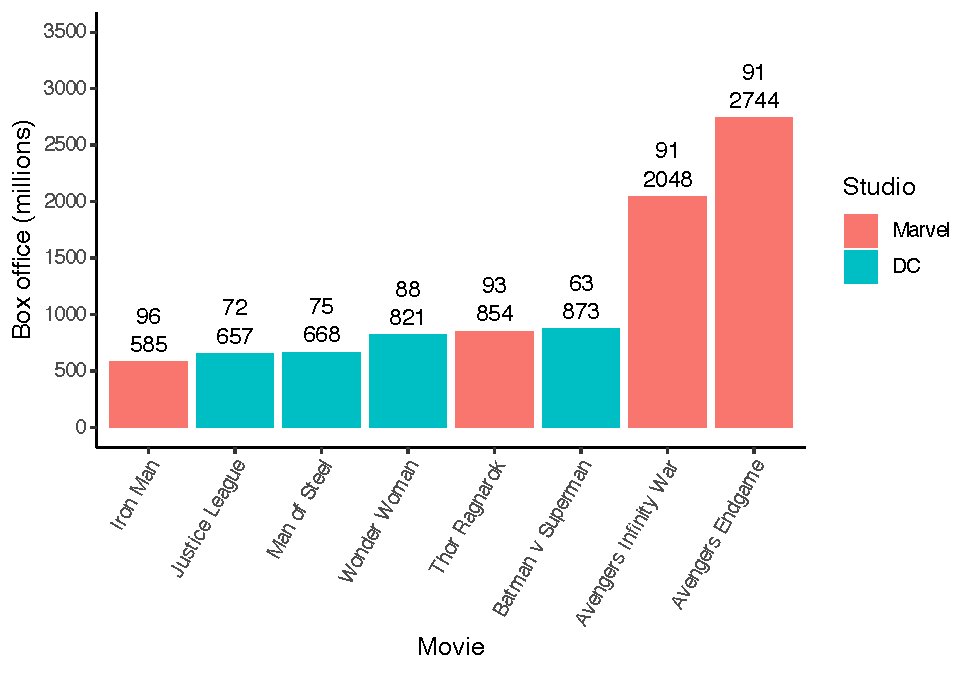
\includegraphics[width=0.65\linewidth]{bookdown_files/figure-latex/unnamed-chunk-133-1}

\subsubsection{Decreasing order}\label{decreasing-order}

We can make the movie bars go left to right in highest to lowest box office receipt order by changing the factor order prior to creating the graph. We use the same code as before but add the desc() command (i.e.,descending) around boxoffice in the fct\_reorder() call:

\begin{Shaded}
\begin{Highlighting}[]
\NormalTok{movie\_data }\OtherTok{\textless{}{-}}\NormalTok{ movie\_data }\SpecialCharTok{\%\textgreater{}\%} \FunctionTok{mutate}\NormalTok{(}\AttributeTok{title =} \FunctionTok{fct\_reorder}\NormalTok{(title,}
                                  \FunctionTok{desc}\NormalTok{(boxoffice)))}
\end{Highlighting}
\end{Shaded}

\begin{Shaded}
\begin{Highlighting}[]
\NormalTok{my\_graph }\OtherTok{\textless{}{-}} \FunctionTok{ggplot}\NormalTok{(}\AttributeTok{data =}\NormalTok{ movie\_data,}
           \AttributeTok{mapping =} \FunctionTok{aes}\NormalTok{(}\AttributeTok{x =}\NormalTok{ title,}
                         \AttributeTok{y =}\NormalTok{ boxoffice,}
                         \AttributeTok{label =}\NormalTok{ boxoffice, }
                         \AttributeTok{fill =}\NormalTok{ studio)) }\SpecialCharTok{+}
  \FunctionTok{geom\_col}\NormalTok{() }\SpecialCharTok{+}
  \FunctionTok{geom\_text}\NormalTok{(}\AttributeTok{nudge\_y =} \DecValTok{150}\NormalTok{)  }\SpecialCharTok{+}
  \FunctionTok{geom\_text}\NormalTok{(}\AttributeTok{mapping =} \FunctionTok{aes}\NormalTok{(}\AttributeTok{label =}\NormalTok{ tomatoes\_aud), }
            \AttributeTok{nudge\_y =} \DecValTok{400}\NormalTok{) }\SpecialCharTok{+}
  \FunctionTok{coord\_cartesian}\NormalTok{(}\AttributeTok{ylim =} \FunctionTok{c}\NormalTok{(}\DecValTok{0}\NormalTok{, }\DecValTok{3500}\NormalTok{)) }\SpecialCharTok{+}
  \FunctionTok{scale\_y\_continuous}\NormalTok{(}\AttributeTok{breaks =} \FunctionTok{seq}\NormalTok{(}\DecValTok{0}\NormalTok{, }\DecValTok{3500}\NormalTok{, }\AttributeTok{by =} \DecValTok{500}\NormalTok{)) }\SpecialCharTok{+}
  \FunctionTok{labs}\NormalTok{(}\AttributeTok{x =} \StringTok{"Movie"}\NormalTok{,}
       \AttributeTok{y =} \StringTok{"Box office (millions)"}\NormalTok{,}
       \AttributeTok{fill =} \StringTok{"Studio"}\NormalTok{) }\SpecialCharTok{+}
  \FunctionTok{theme\_classic}\NormalTok{(}\DecValTok{12}\NormalTok{) }\SpecialCharTok{+}
  \FunctionTok{theme}\NormalTok{(}\AttributeTok{axis.text.x =} \FunctionTok{element\_text}\NormalTok{(}\AttributeTok{angle =} \DecValTok{60}\NormalTok{, }
                                   \AttributeTok{hjust =} \DecValTok{1}\NormalTok{))  }

\FunctionTok{print}\NormalTok{(my\_graph)}
\end{Highlighting}
\end{Shaded}

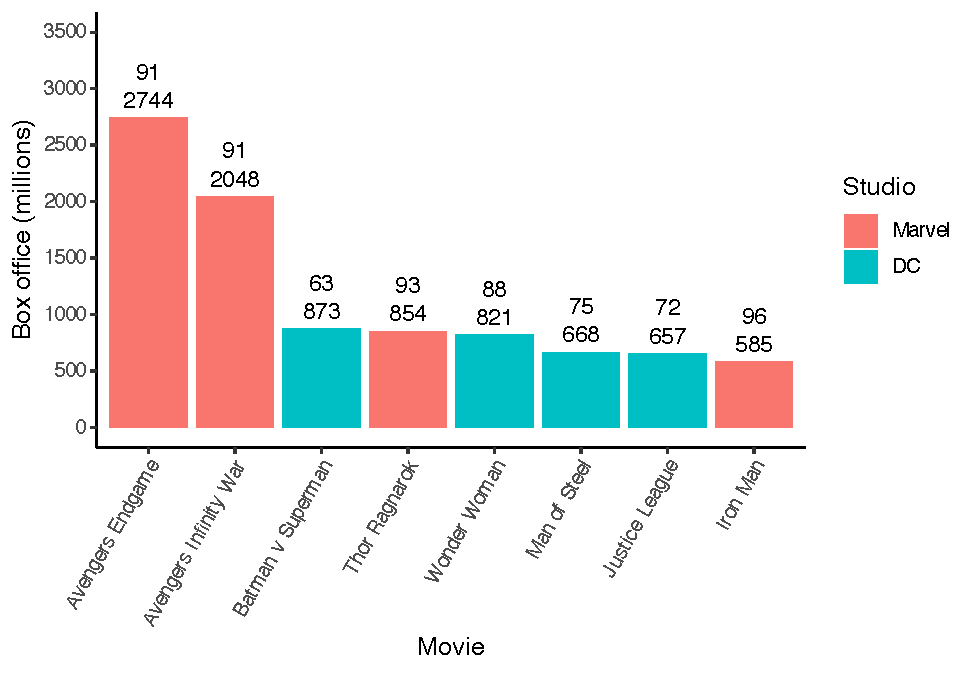
\includegraphics[width=0.65\linewidth]{bookdown_files/figure-latex/unnamed-chunk-135-1}

\subsubsection{Custom order}\label{custom-order}

We can make the movie bars go left to right in a custom order by changing the factor order prior to creating the graph. Because we want a custom order of the factor levels we use fct\_relevel(), instead of the the fct\_reorder() command from the previous two examples. Below I use this approach to manually order movies highest to lowest boxoffice within movie studio (Marvel or DC).

\begin{Shaded}
\begin{Highlighting}[]
\NormalTok{movie\_data }\OtherTok{\textless{}{-}}\NormalTok{ movie\_data }\SpecialCharTok{\%\textgreater{}\%} 
  \FunctionTok{mutate}\NormalTok{(}\AttributeTok{title =} \FunctionTok{fct\_relevel}\NormalTok{(title,}
                             \StringTok{"Avengers Endgame"}\NormalTok{,}
                             \StringTok{"Avengers Infinity War"}\NormalTok{,}
                             \StringTok{"Thor Ragnarok"}\NormalTok{,}
                             \StringTok{"Iron Man"}\NormalTok{,}
                             \StringTok{"Batman v Superman"}\NormalTok{,}
                             \StringTok{"Wonder Woman"}\NormalTok{,}
                             \StringTok{"Man of Steel"}\NormalTok{,}
                             \StringTok{"Justice League"}\NormalTok{))}
\end{Highlighting}
\end{Shaded}

\begin{Shaded}
\begin{Highlighting}[]
\NormalTok{my\_graph }\OtherTok{\textless{}{-}} \FunctionTok{ggplot}\NormalTok{(}\AttributeTok{data =}\NormalTok{ movie\_data,}
           \AttributeTok{mapping =} \FunctionTok{aes}\NormalTok{(}\AttributeTok{x =}\NormalTok{ title,}
                         \AttributeTok{y =}\NormalTok{ boxoffice,}
                         \AttributeTok{label =}\NormalTok{ boxoffice, }
                         \AttributeTok{fill =}\NormalTok{ studio)) }\SpecialCharTok{+}
  \FunctionTok{geom\_col}\NormalTok{() }\SpecialCharTok{+}
  \FunctionTok{geom\_text}\NormalTok{(}\AttributeTok{nudge\_y =} \DecValTok{150}\NormalTok{)  }\SpecialCharTok{+}
  \FunctionTok{geom\_text}\NormalTok{(}\AttributeTok{mapping =} \FunctionTok{aes}\NormalTok{(}\AttributeTok{label =}\NormalTok{ tomatoes\_aud), }
            \AttributeTok{nudge\_y =} \DecValTok{400}\NormalTok{) }\SpecialCharTok{+}
  \FunctionTok{coord\_cartesian}\NormalTok{(}\AttributeTok{ylim =} \FunctionTok{c}\NormalTok{(}\DecValTok{0}\NormalTok{, }\DecValTok{3500}\NormalTok{)) }\SpecialCharTok{+}
  \FunctionTok{scale\_y\_continuous}\NormalTok{(}\AttributeTok{breaks =} \FunctionTok{seq}\NormalTok{(}\DecValTok{0}\NormalTok{, }\DecValTok{3500}\NormalTok{, }\AttributeTok{by =} \DecValTok{500}\NormalTok{)) }\SpecialCharTok{+}
  \FunctionTok{labs}\NormalTok{(}\AttributeTok{x =} \StringTok{"Movie"}\NormalTok{,}
       \AttributeTok{y =} \StringTok{"Box office (millions)"}\NormalTok{,}
       \AttributeTok{fill =} \StringTok{"Studio"}\NormalTok{) }\SpecialCharTok{+}
  \FunctionTok{theme\_classic}\NormalTok{(}\DecValTok{12}\NormalTok{) }\SpecialCharTok{+}
  \FunctionTok{theme}\NormalTok{(}\AttributeTok{axis.text.x =} \FunctionTok{element\_text}\NormalTok{(}\AttributeTok{angle =} \DecValTok{60}\NormalTok{, }
                                   \AttributeTok{hjust =} \DecValTok{1}\NormalTok{))  }
\end{Highlighting}
\end{Shaded}

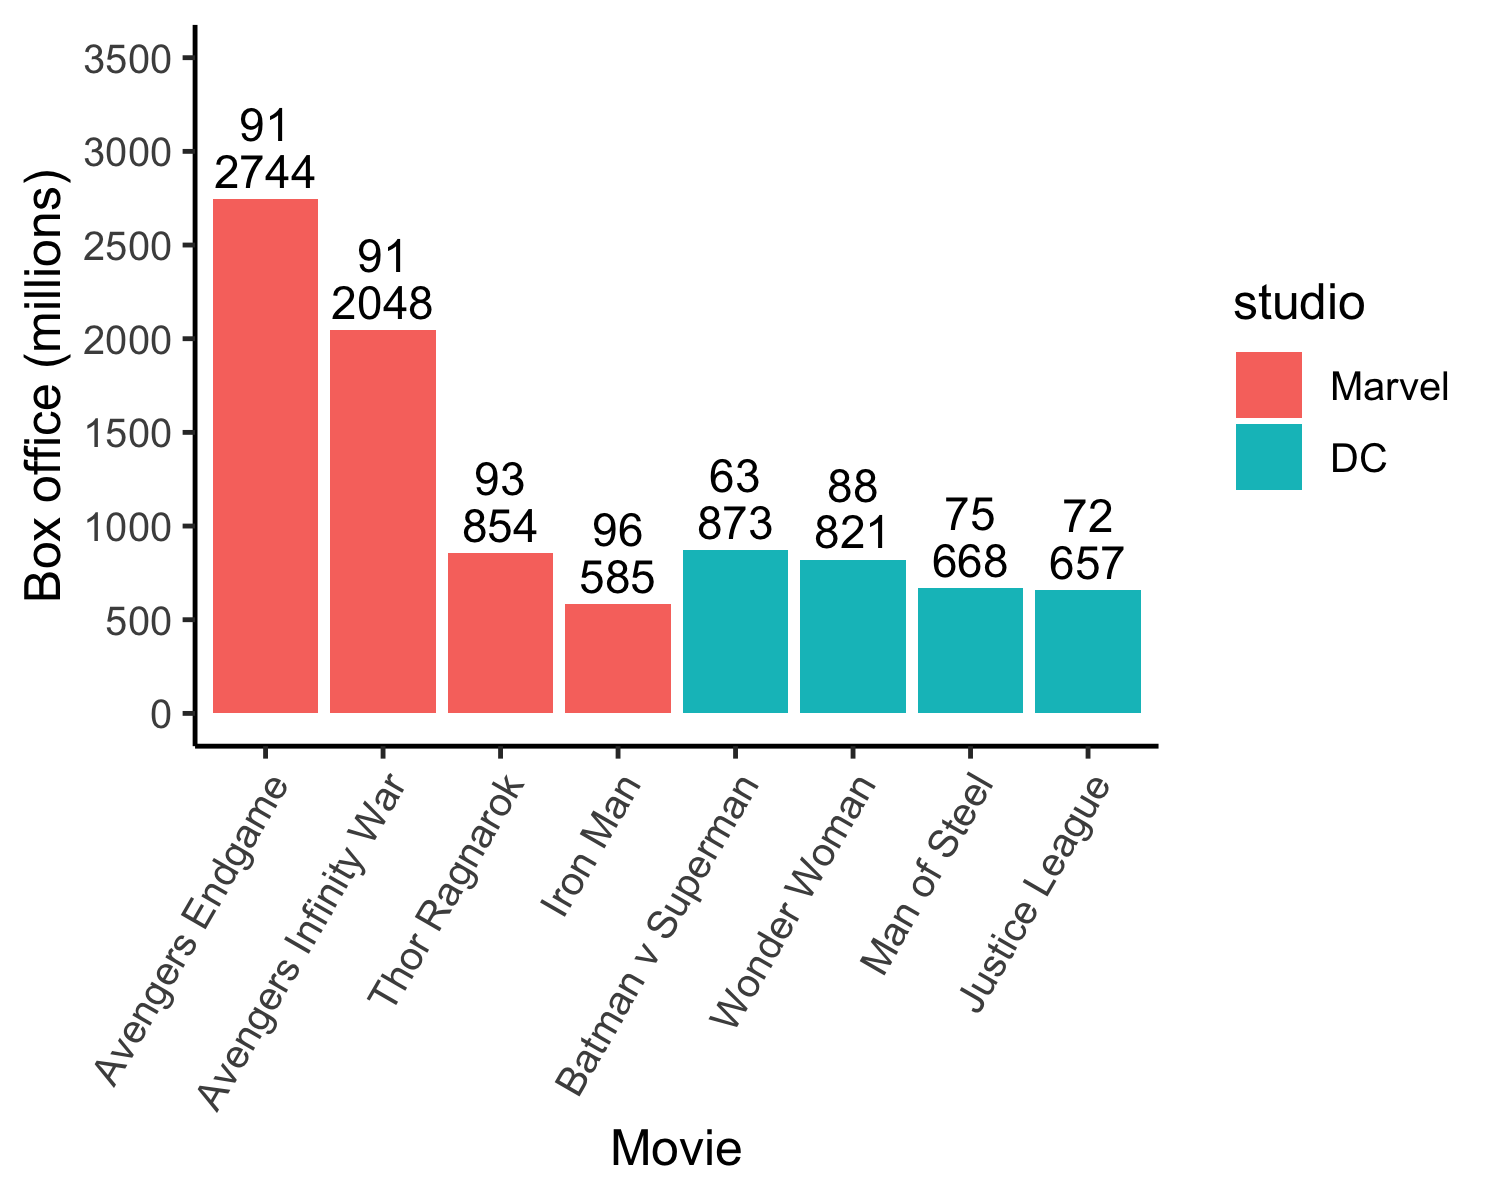
\includegraphics[width=0.65\linewidth]{ch_graphing/images/custom_order}

\subsection{Legend order}\label{legend-order}

After inspecting the graph on the previous page, you might think that Marvel should be above DC in the legend. You can do that by reordering the studio factor:

\begin{Shaded}
\begin{Highlighting}[]
\NormalTok{movie\_data }\OtherTok{\textless{}{-}}\NormalTok{ movie\_data }\SpecialCharTok{\%\textgreater{}\%} 
  \FunctionTok{mutate}\NormalTok{(}\AttributeTok{studio =} \FunctionTok{fct\_relevel}\NormalTok{(studio,}
                             \StringTok{"Marvel"}\NormalTok{,}
                             \StringTok{"DC"}\NormalTok{))}
\end{Highlighting}
\end{Shaded}

\begin{Shaded}
\begin{Highlighting}[]
\NormalTok{my\_graph }\OtherTok{\textless{}{-}} \FunctionTok{ggplot}\NormalTok{(}\AttributeTok{data =}\NormalTok{ movie\_data,}
           \AttributeTok{mapping =} \FunctionTok{aes}\NormalTok{(}\AttributeTok{x =}\NormalTok{ title,}
                         \AttributeTok{y =}\NormalTok{ boxoffice,}
                         \AttributeTok{label =}\NormalTok{ boxoffice, }
                         \AttributeTok{fill =}\NormalTok{ studio)) }\SpecialCharTok{+}
  \FunctionTok{geom\_col}\NormalTok{() }\SpecialCharTok{+}
  \FunctionTok{geom\_text}\NormalTok{(}\AttributeTok{nudge\_y =} \DecValTok{150}\NormalTok{)  }\SpecialCharTok{+}
  \FunctionTok{geom\_text}\NormalTok{(}\AttributeTok{mapping =} \FunctionTok{aes}\NormalTok{(}\AttributeTok{label =}\NormalTok{ tomatoes\_aud), }
            \AttributeTok{nudge\_y =} \DecValTok{400}\NormalTok{) }\SpecialCharTok{+}
  \FunctionTok{coord\_cartesian}\NormalTok{(}\AttributeTok{ylim =} \FunctionTok{c}\NormalTok{(}\DecValTok{0}\NormalTok{, }\DecValTok{3500}\NormalTok{)) }\SpecialCharTok{+}
  \FunctionTok{scale\_y\_continuous}\NormalTok{(}\AttributeTok{breaks =} \FunctionTok{seq}\NormalTok{(}\DecValTok{0}\NormalTok{, }\DecValTok{3500}\NormalTok{, }\AttributeTok{by =} \DecValTok{500}\NormalTok{)) }\SpecialCharTok{+}
  \FunctionTok{labs}\NormalTok{(}\AttributeTok{x =} \StringTok{"Movie"}\NormalTok{,}
       \AttributeTok{y =} \StringTok{"Box office (millions)"}\NormalTok{,}
       \AttributeTok{fill =} \StringTok{"Studio"}\NormalTok{) }\SpecialCharTok{+}
  \FunctionTok{theme\_classic}\NormalTok{(}\DecValTok{12}\NormalTok{) }\SpecialCharTok{+}
  \FunctionTok{theme}\NormalTok{(}\AttributeTok{axis.text.x =} \FunctionTok{element\_text}\NormalTok{(}\AttributeTok{angle =} \DecValTok{60}\NormalTok{, }
                                   \AttributeTok{hjust =} \DecValTok{1}\NormalTok{))  }
\end{Highlighting}
\end{Shaded}

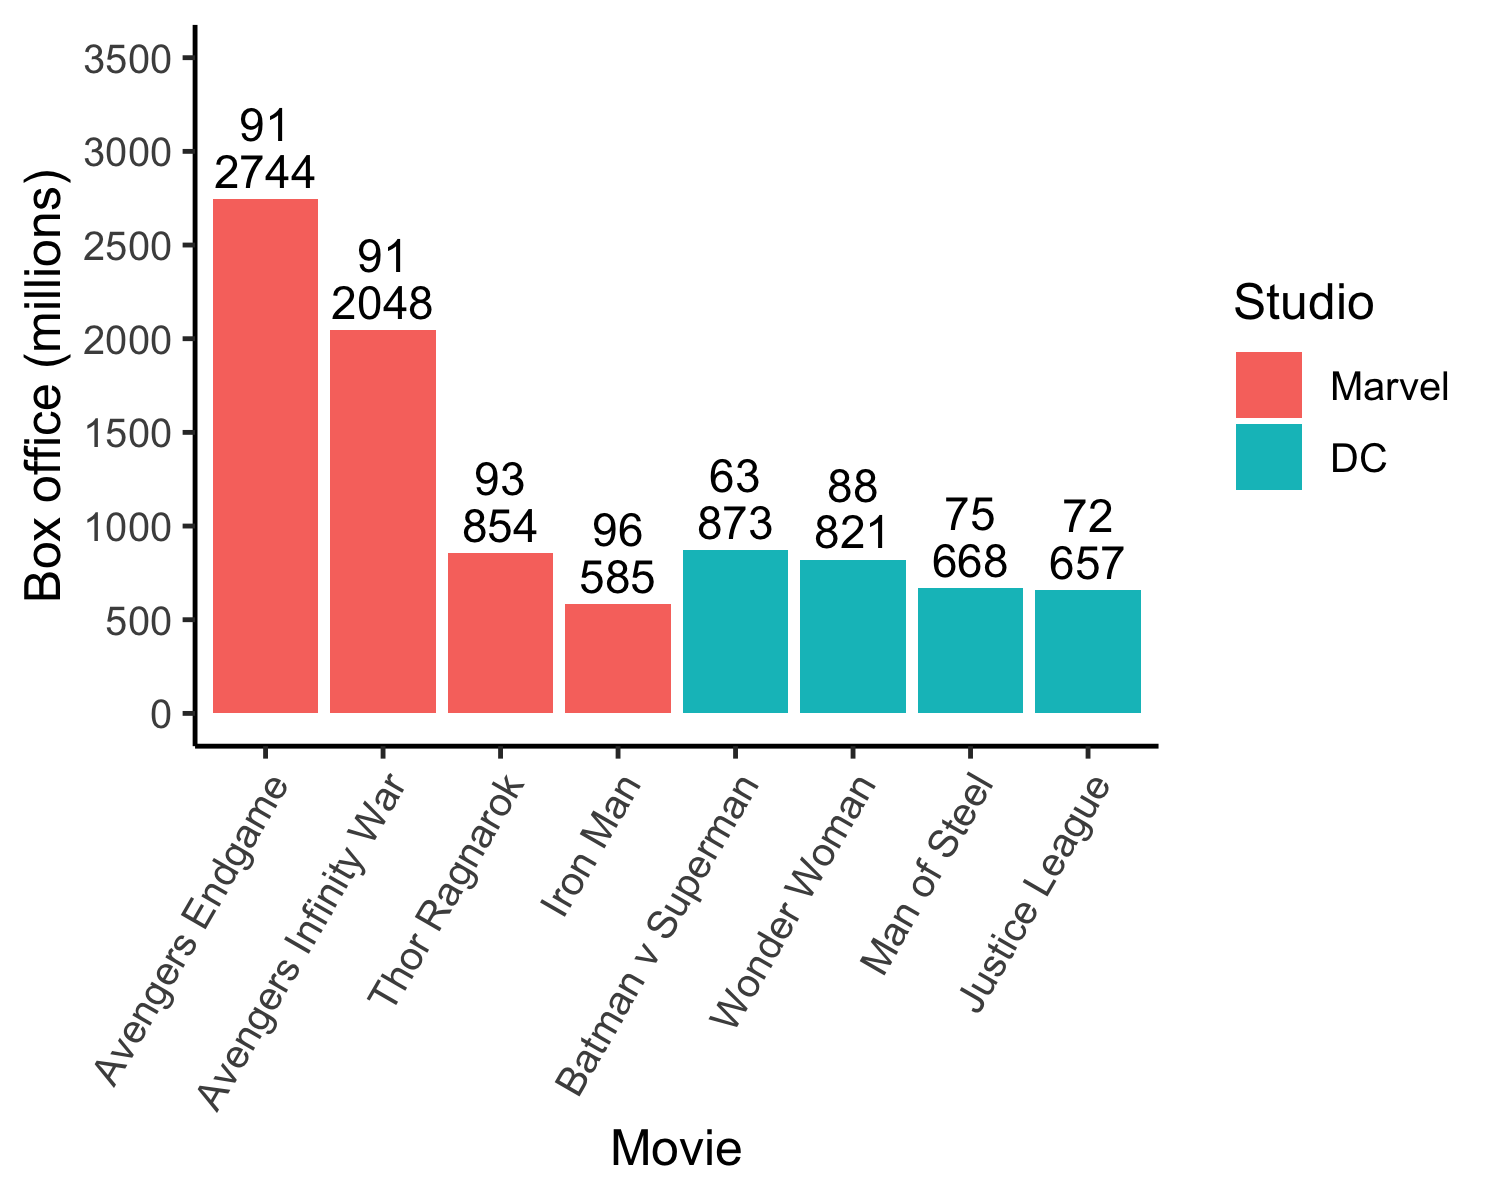
\includegraphics[width=0.65\linewidth]{ch_graphing/images/custom_order2}

\section{Custom colours}\label{custom-colours}

\subsection{R palette}\label{r-palette}

You might look at the previous graph and think ``Marvel should be red and DC should be blue since those are the colours of their respective logos''. You can do that with the code below. Note that you specify the colours in the order the names appear in the legend (top to bottom).

R colour names/pictures can be found here: \url{http://sape.inf.usi.ch/quick-reference/ggplot2/colour}

\begin{Shaded}
\begin{Highlighting}[]
\NormalTok{my\_graph }\OtherTok{\textless{}{-}} \FunctionTok{ggplot}\NormalTok{(}\AttributeTok{data =}\NormalTok{ movie\_data,}
           \AttributeTok{mapping =} \FunctionTok{aes}\NormalTok{(}\AttributeTok{x =}\NormalTok{ title,}
                         \AttributeTok{y =}\NormalTok{ boxoffice,}
                         \AttributeTok{label =}\NormalTok{ boxoffice, }
                         \AttributeTok{fill =}\NormalTok{ studio)) }\SpecialCharTok{+}
  \FunctionTok{geom\_col}\NormalTok{() }\SpecialCharTok{+}
  \FunctionTok{geom\_text}\NormalTok{(}\AttributeTok{nudge\_y =} \DecValTok{150}\NormalTok{)  }\SpecialCharTok{+}
  \FunctionTok{geom\_text}\NormalTok{(}\AttributeTok{mapping =} \FunctionTok{aes}\NormalTok{(}\AttributeTok{label =}\NormalTok{ tomatoes\_aud), }
            \AttributeTok{nudge\_y =} \DecValTok{400}\NormalTok{) }\SpecialCharTok{+}
  \FunctionTok{coord\_cartesian}\NormalTok{(}\AttributeTok{ylim =} \FunctionTok{c}\NormalTok{(}\DecValTok{0}\NormalTok{, }\DecValTok{3500}\NormalTok{)) }\SpecialCharTok{+}
  \FunctionTok{scale\_y\_continuous}\NormalTok{(}\AttributeTok{breaks =} \FunctionTok{seq}\NormalTok{(}\DecValTok{0}\NormalTok{, }\DecValTok{3500}\NormalTok{, }\AttributeTok{by =} \DecValTok{500}\NormalTok{)) }\SpecialCharTok{+}
  \FunctionTok{labs}\NormalTok{(}\AttributeTok{x =} \StringTok{"Movie"}\NormalTok{,}
       \AttributeTok{y =} \StringTok{"Box office (millions)"}\NormalTok{,}
       \AttributeTok{fill =} \StringTok{"Studio"}\NormalTok{) }\SpecialCharTok{+}
  \FunctionTok{theme\_classic}\NormalTok{(}\DecValTok{12}\NormalTok{) }\SpecialCharTok{+}
  \FunctionTok{theme}\NormalTok{(}\AttributeTok{axis.text.x =} \FunctionTok{element\_text}\NormalTok{(}\AttributeTok{angle =} \DecValTok{60}\NormalTok{, }
                                   \AttributeTok{hjust =} \DecValTok{1}\NormalTok{)) }\SpecialCharTok{+}
  \FunctionTok{scale\_fill\_manual}\NormalTok{(}\AttributeTok{values =} \FunctionTok{c}\NormalTok{(}\StringTok{"red"}\NormalTok{, }\StringTok{"blue"}\NormalTok{))}
\end{Highlighting}
\end{Shaded}

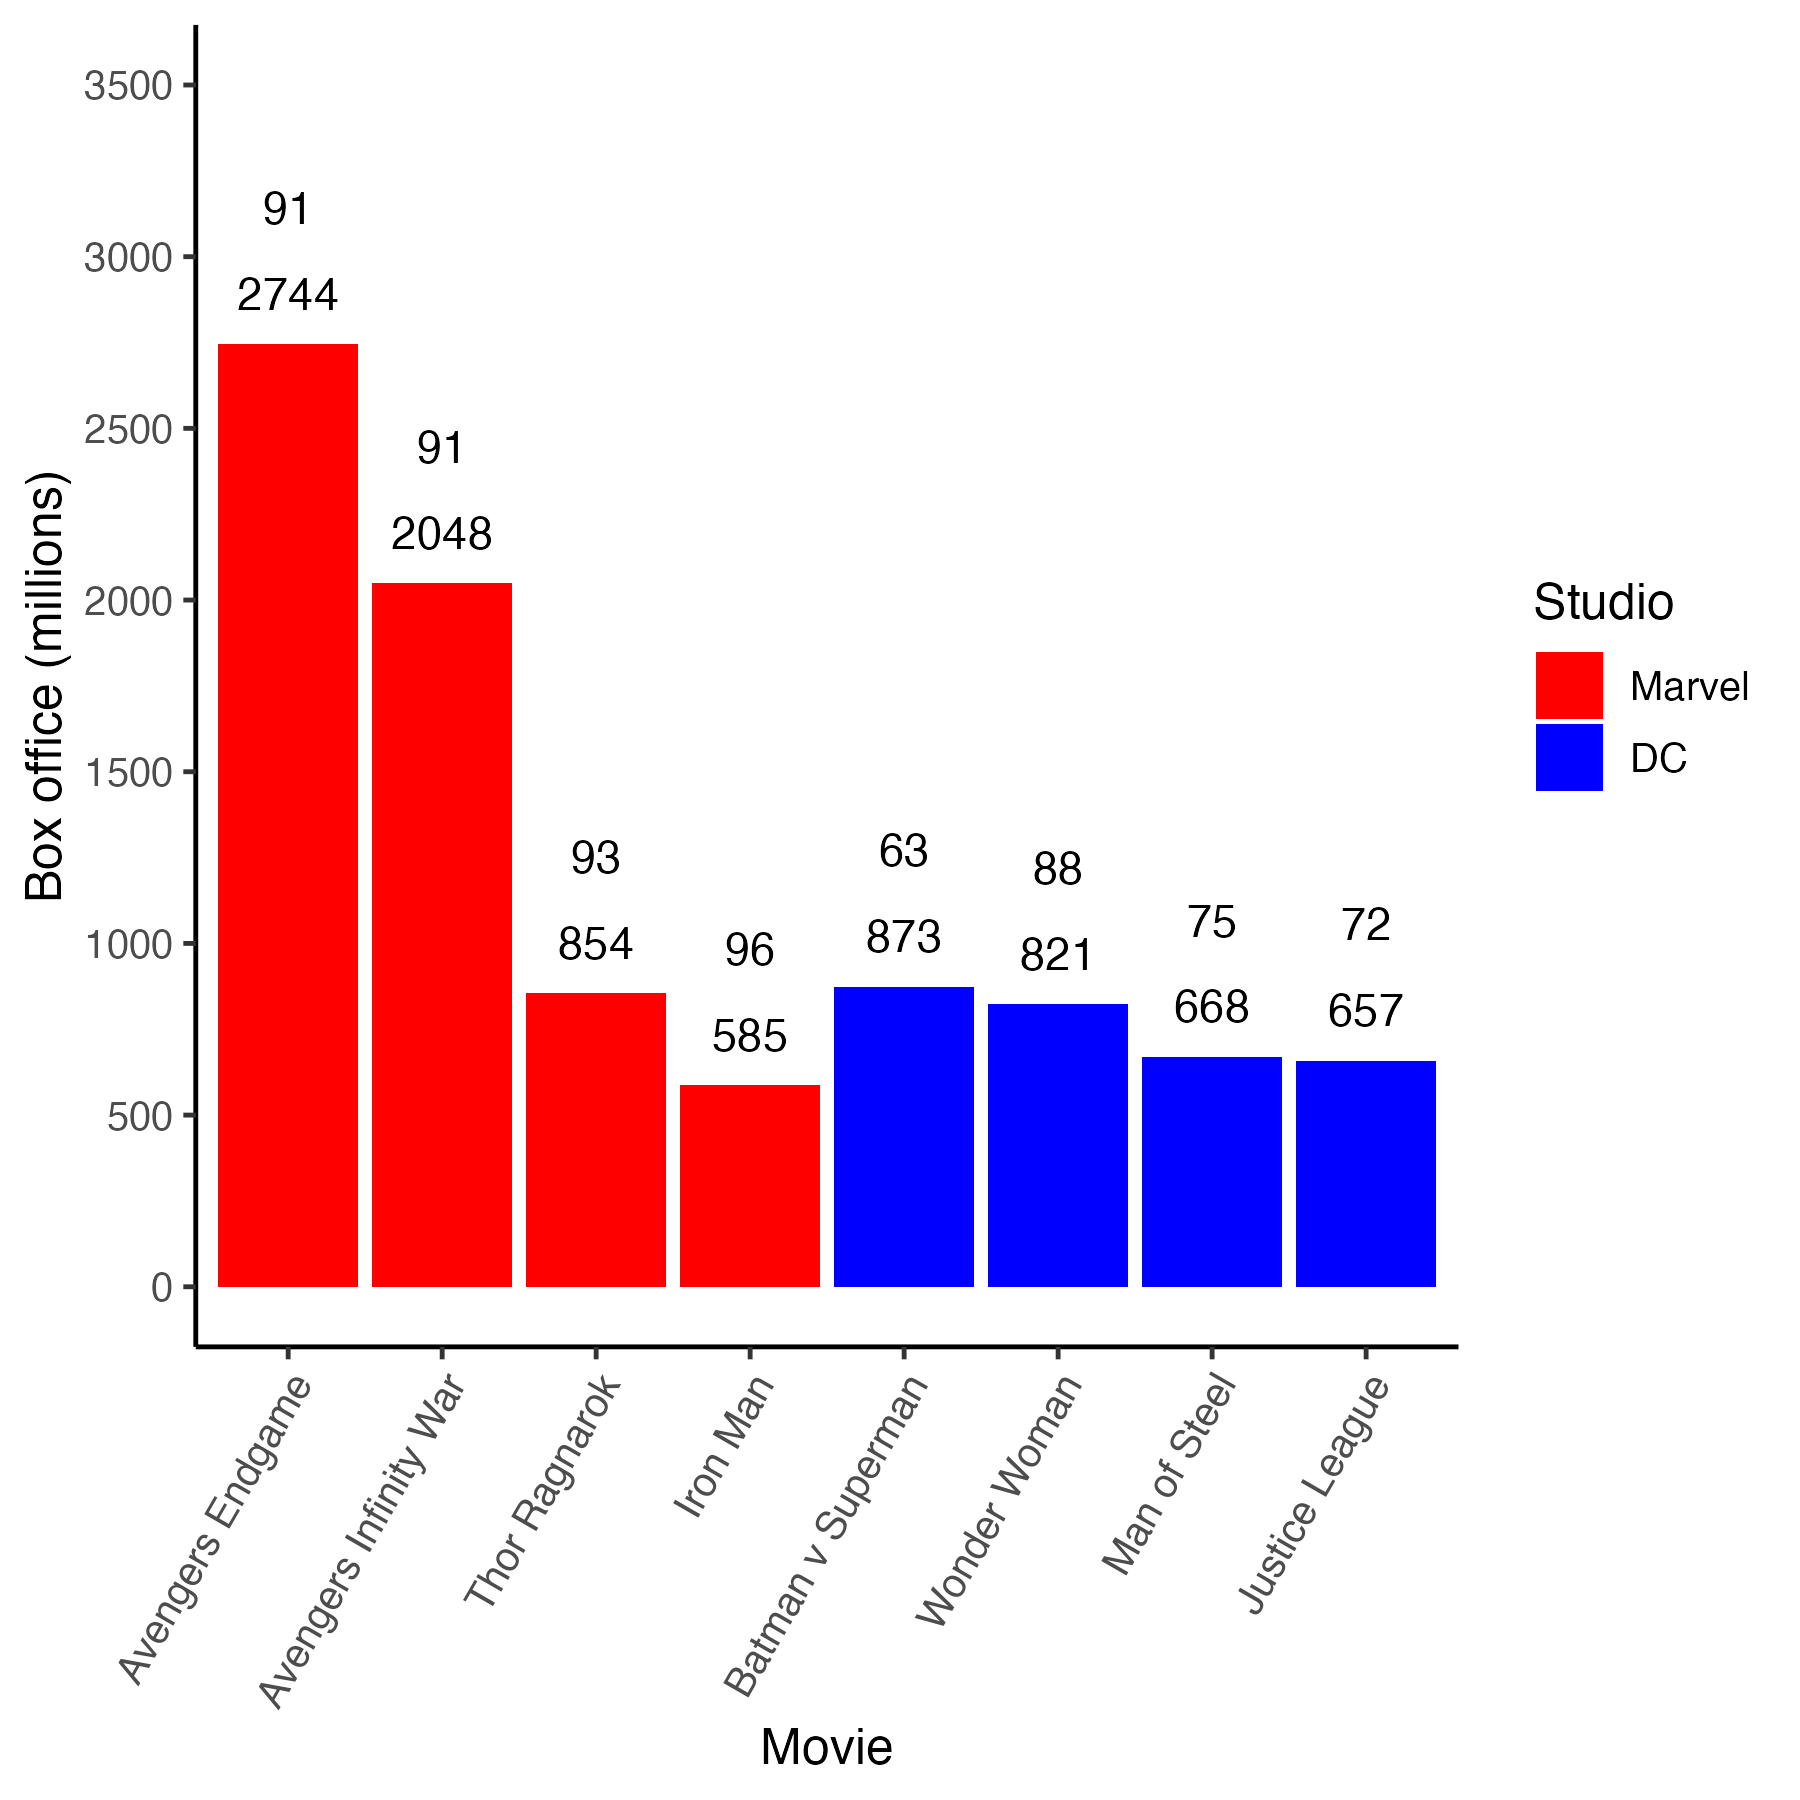
\includegraphics[width=0.65\linewidth]{ch_graphing/images/base_color_graph}

\subsection{Hex colours}\label{hex-colours}

If you are a really big geek (like me) you might look at the previous graph and think ``Those aren't the proper colours for the Marvel and DC - lame!'' So\ldots{} you do some internet research and determine that you can specify colours using hexidecimal numbers. More specifically, you find Marvel red is \#ed1d24 and DC blue is \#0476F2 using hex colour codes. You can use those precise colours via the scale\_fill\_manual() command below.

\begin{Shaded}
\begin{Highlighting}[]
\NormalTok{my\_graph }\OtherTok{\textless{}{-}} \FunctionTok{ggplot}\NormalTok{(}\AttributeTok{data =}\NormalTok{ movie\_data,}
           \AttributeTok{mapping =} \FunctionTok{aes}\NormalTok{(}\AttributeTok{x =}\NormalTok{ title,}
                         \AttributeTok{y =}\NormalTok{ boxoffice,}
                         \AttributeTok{label =}\NormalTok{ boxoffice, }
                         \AttributeTok{fill =}\NormalTok{ studio)) }\SpecialCharTok{+}
  \FunctionTok{geom\_col}\NormalTok{() }\SpecialCharTok{+}
  \FunctionTok{geom\_text}\NormalTok{(}\AttributeTok{nudge\_y =} \DecValTok{150}\NormalTok{)  }\SpecialCharTok{+}
  \FunctionTok{geom\_text}\NormalTok{(}\AttributeTok{mapping =} \FunctionTok{aes}\NormalTok{(}\AttributeTok{label =}\NormalTok{ tomatoes\_aud), }
            \AttributeTok{nudge\_y =} \DecValTok{400}\NormalTok{) }\SpecialCharTok{+}
  \FunctionTok{coord\_cartesian}\NormalTok{(}\AttributeTok{ylim =} \FunctionTok{c}\NormalTok{(}\DecValTok{0}\NormalTok{, }\DecValTok{3500}\NormalTok{)) }\SpecialCharTok{+}
  \FunctionTok{scale\_y\_continuous}\NormalTok{(}\AttributeTok{breaks =} \FunctionTok{seq}\NormalTok{(}\DecValTok{0}\NormalTok{, }\DecValTok{3500}\NormalTok{, }\AttributeTok{by =} \DecValTok{500}\NormalTok{)) }\SpecialCharTok{+}
  \FunctionTok{labs}\NormalTok{(}\AttributeTok{x =} \StringTok{"Movie"}\NormalTok{,}
       \AttributeTok{y =} \StringTok{"Box office (millions)"}\NormalTok{,}
       \AttributeTok{fill =} \StringTok{"Studio"}\NormalTok{) }\SpecialCharTok{+}
  \FunctionTok{theme\_classic}\NormalTok{(}\DecValTok{12}\NormalTok{) }\SpecialCharTok{+}
  \FunctionTok{theme}\NormalTok{(}\AttributeTok{axis.text.x =} \FunctionTok{element\_text}\NormalTok{(}\AttributeTok{angle =} \DecValTok{60}\NormalTok{, }
                                   \AttributeTok{hjust =} \DecValTok{1}\NormalTok{)) }\SpecialCharTok{+}
  \FunctionTok{scale\_fill\_manual}\NormalTok{(}\AttributeTok{values =} \FunctionTok{c}\NormalTok{(}\StringTok{"\#ed1d24"}\NormalTok{, }\StringTok{"\#0476F2"}\NormalTok{))}
\end{Highlighting}
\end{Shaded}

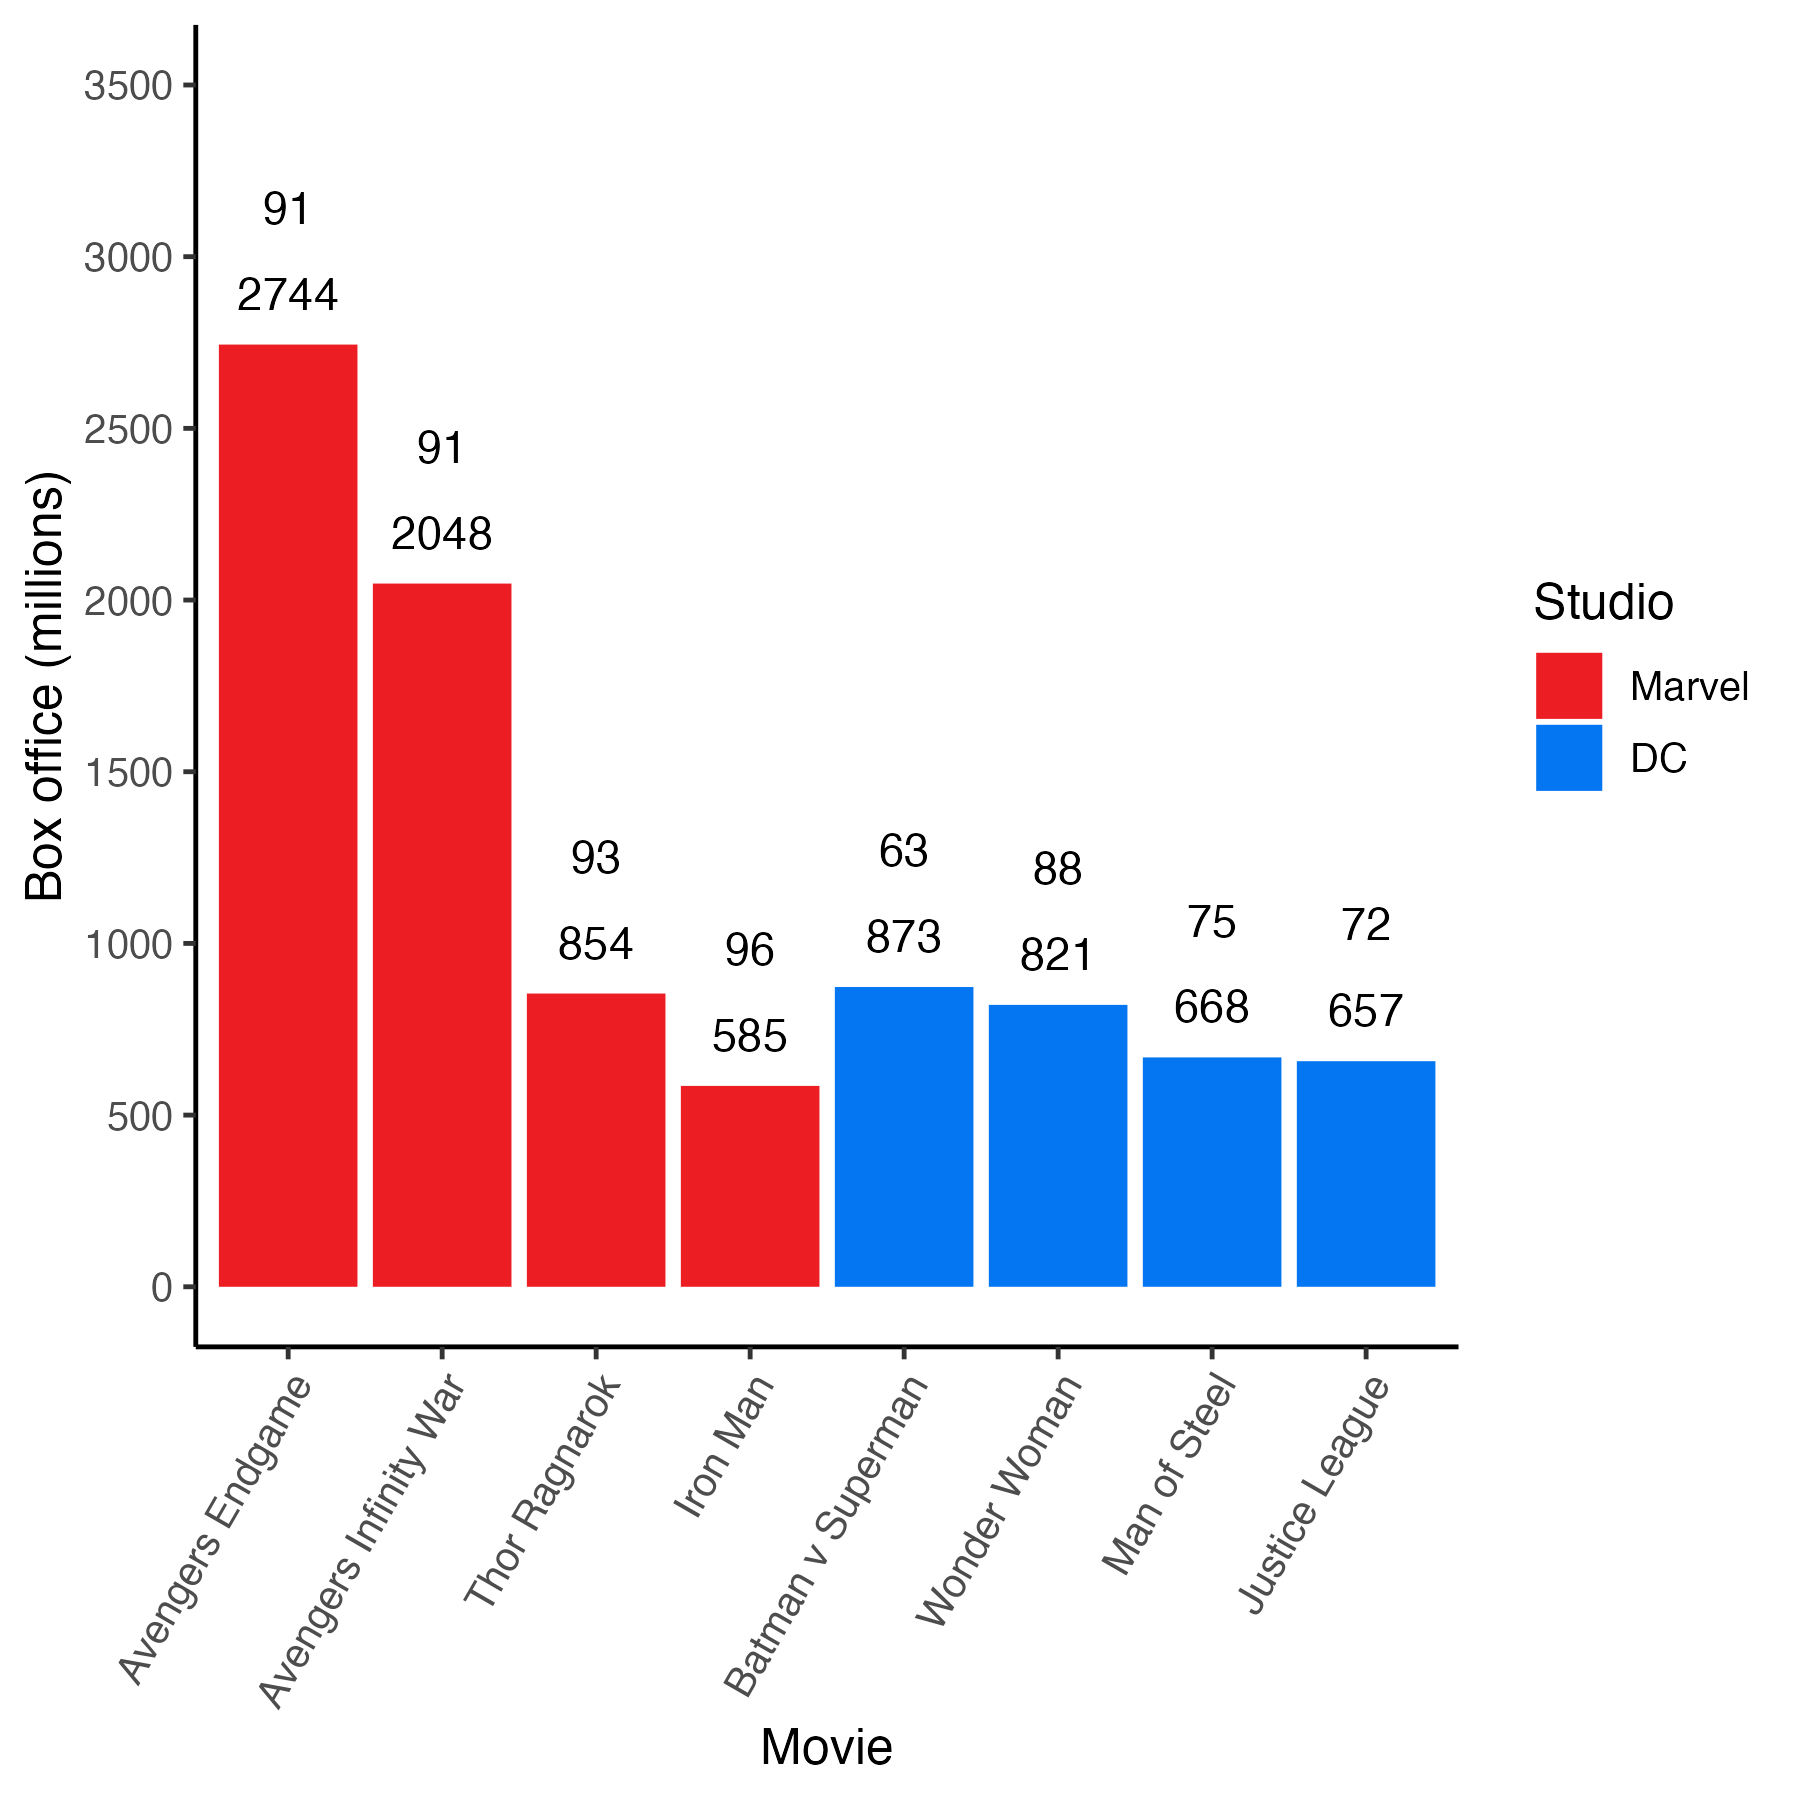
\includegraphics[width=0.65\linewidth]{ch_graphing/images/logo_color_graph}

\section{Emoji}\label{emoji}

Make the graph more fun with the emoGG package. You might like to make the graph more fun by putting tomatoes on the graph to indicate what the extra numbers mean. We can do that with the emoGG package. The installation instructions for this package are at the start of this chapter; note, that it is installed via GitHub rather than the CRAN. Course R Studio Cloud users - the installation has already been done.

After installation you need to activate the emoGG package:

\begin{Shaded}
\begin{Highlighting}[]
\FunctionTok{library}\NormalTok{(emoGG)}
\end{Highlighting}
\end{Shaded}

Visit this link to check out the codes for emoji: \url{https://apps.timwhitlock.info/emoji/tables/unicode}

If you scroll down to section 5 Uncategorized on this page you will find the code for a tomato is 1f345. Note that the code below will only work with an internet connection. The command geom\_emoji() needs internet access to retrieve the emoji graphic requested.

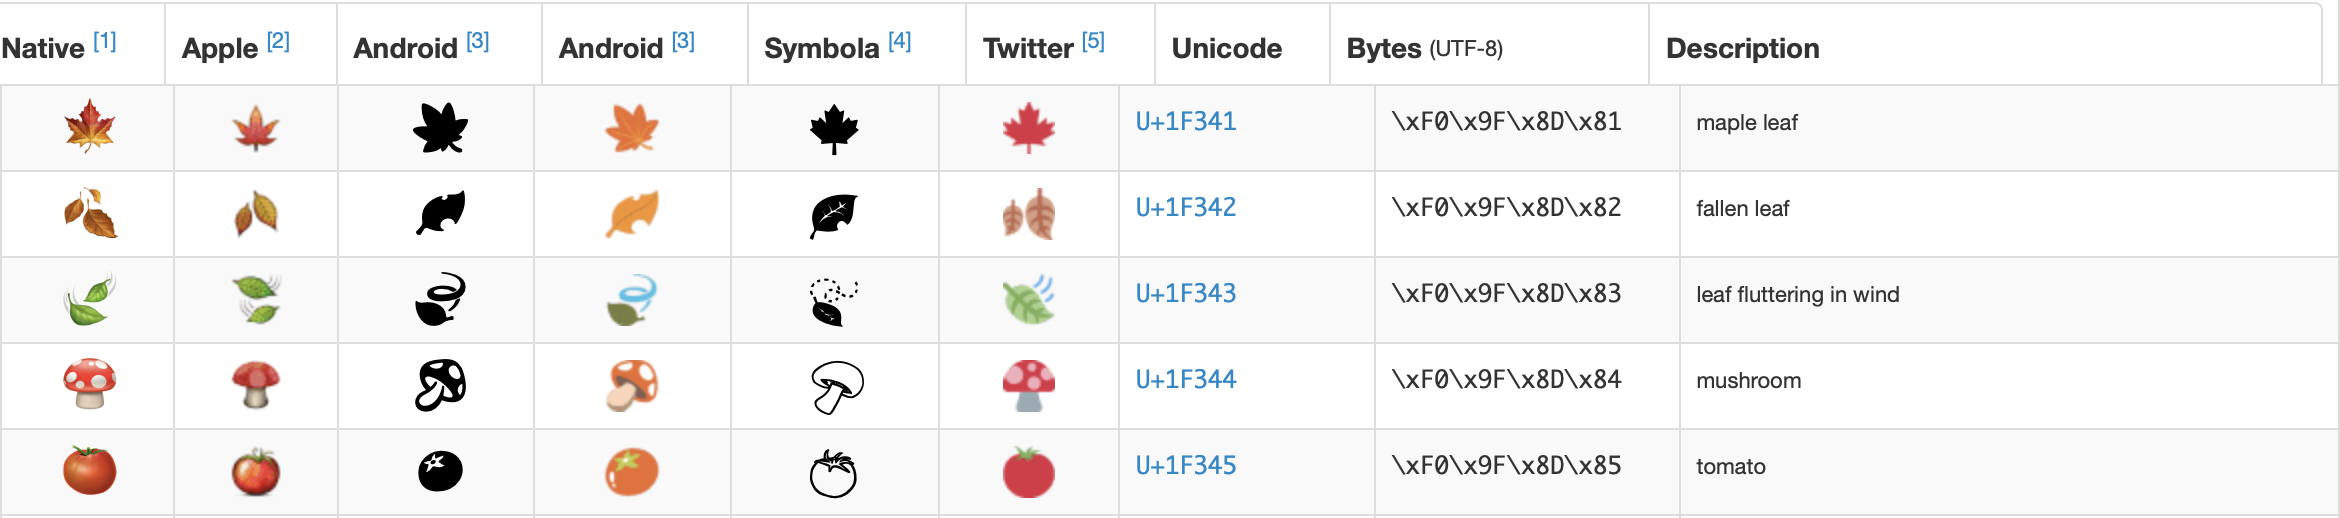
\includegraphics[width=0.9\linewidth]{ch_graphing/images/emoji_table}

\begin{Shaded}
\begin{Highlighting}[]
\NormalTok{my\_graph }\OtherTok{\textless{}{-}} \FunctionTok{ggplot}\NormalTok{(}\AttributeTok{data =}\NormalTok{ movie\_data,}
           \AttributeTok{mapping =} \FunctionTok{aes}\NormalTok{(}\AttributeTok{x =}\NormalTok{ title,}
                         \AttributeTok{y =}\NormalTok{ boxoffice,}
                         \AttributeTok{label =}\NormalTok{ boxoffice, }
                         \AttributeTok{fill =}\NormalTok{ studio)) }\SpecialCharTok{+}
  \FunctionTok{geom\_col}\NormalTok{() }\SpecialCharTok{+}
  \FunctionTok{geom\_text}\NormalTok{(}\AttributeTok{nudge\_y =} \DecValTok{150}\NormalTok{)  }\SpecialCharTok{+}
  \FunctionTok{geom\_text}\NormalTok{(}\AttributeTok{mapping =} \FunctionTok{aes}\NormalTok{(}\AttributeTok{label =}\NormalTok{ tomatoes\_aud), }
            \AttributeTok{nudge\_y =} \DecValTok{600}\NormalTok{, }
            \AttributeTok{colour =} \StringTok{"red"}\NormalTok{) }\SpecialCharTok{+}
  \FunctionTok{geom\_emoji}\NormalTok{(}\AttributeTok{mapping =} \FunctionTok{aes}\NormalTok{(}\AttributeTok{y =}\NormalTok{ boxoffice }\SpecialCharTok{+} \DecValTok{400}\NormalTok{),}
             \AttributeTok{emoji=}\StringTok{"1f345"}\NormalTok{) }\SpecialCharTok{+}
  \FunctionTok{coord\_cartesian}\NormalTok{(}\AttributeTok{ylim =} \FunctionTok{c}\NormalTok{(}\DecValTok{0}\NormalTok{, }\DecValTok{3500}\NormalTok{)) }\SpecialCharTok{+}
  \FunctionTok{scale\_y\_continuous}\NormalTok{(}\AttributeTok{breaks =} \FunctionTok{seq}\NormalTok{(}\DecValTok{0}\NormalTok{, }\DecValTok{3500}\NormalTok{, }\AttributeTok{by =} \DecValTok{500}\NormalTok{)) }\SpecialCharTok{+}
  \FunctionTok{labs}\NormalTok{(}\AttributeTok{x =} \StringTok{"Movie"}\NormalTok{,}
       \AttributeTok{y =} \StringTok{"Box office (millions)"}\NormalTok{,}
       \AttributeTok{fill =} \StringTok{"Studio"}\NormalTok{) }\SpecialCharTok{+}
  \FunctionTok{theme\_classic}\NormalTok{(}\DecValTok{12}\NormalTok{) }\SpecialCharTok{+}
  \FunctionTok{theme}\NormalTok{(}\AttributeTok{axis.text.x =} \FunctionTok{element\_text}\NormalTok{(}\AttributeTok{angle =} \DecValTok{60}\NormalTok{, }
                                   \AttributeTok{hjust =} \DecValTok{1}\NormalTok{)) }\SpecialCharTok{+}
  \FunctionTok{scale\_fill\_manual}\NormalTok{(}\AttributeTok{values =} \FunctionTok{c}\NormalTok{(}\StringTok{"\#ed1d24"}\NormalTok{, }\StringTok{"\#0476F2"}\NormalTok{))}
\end{Highlighting}
\end{Shaded}

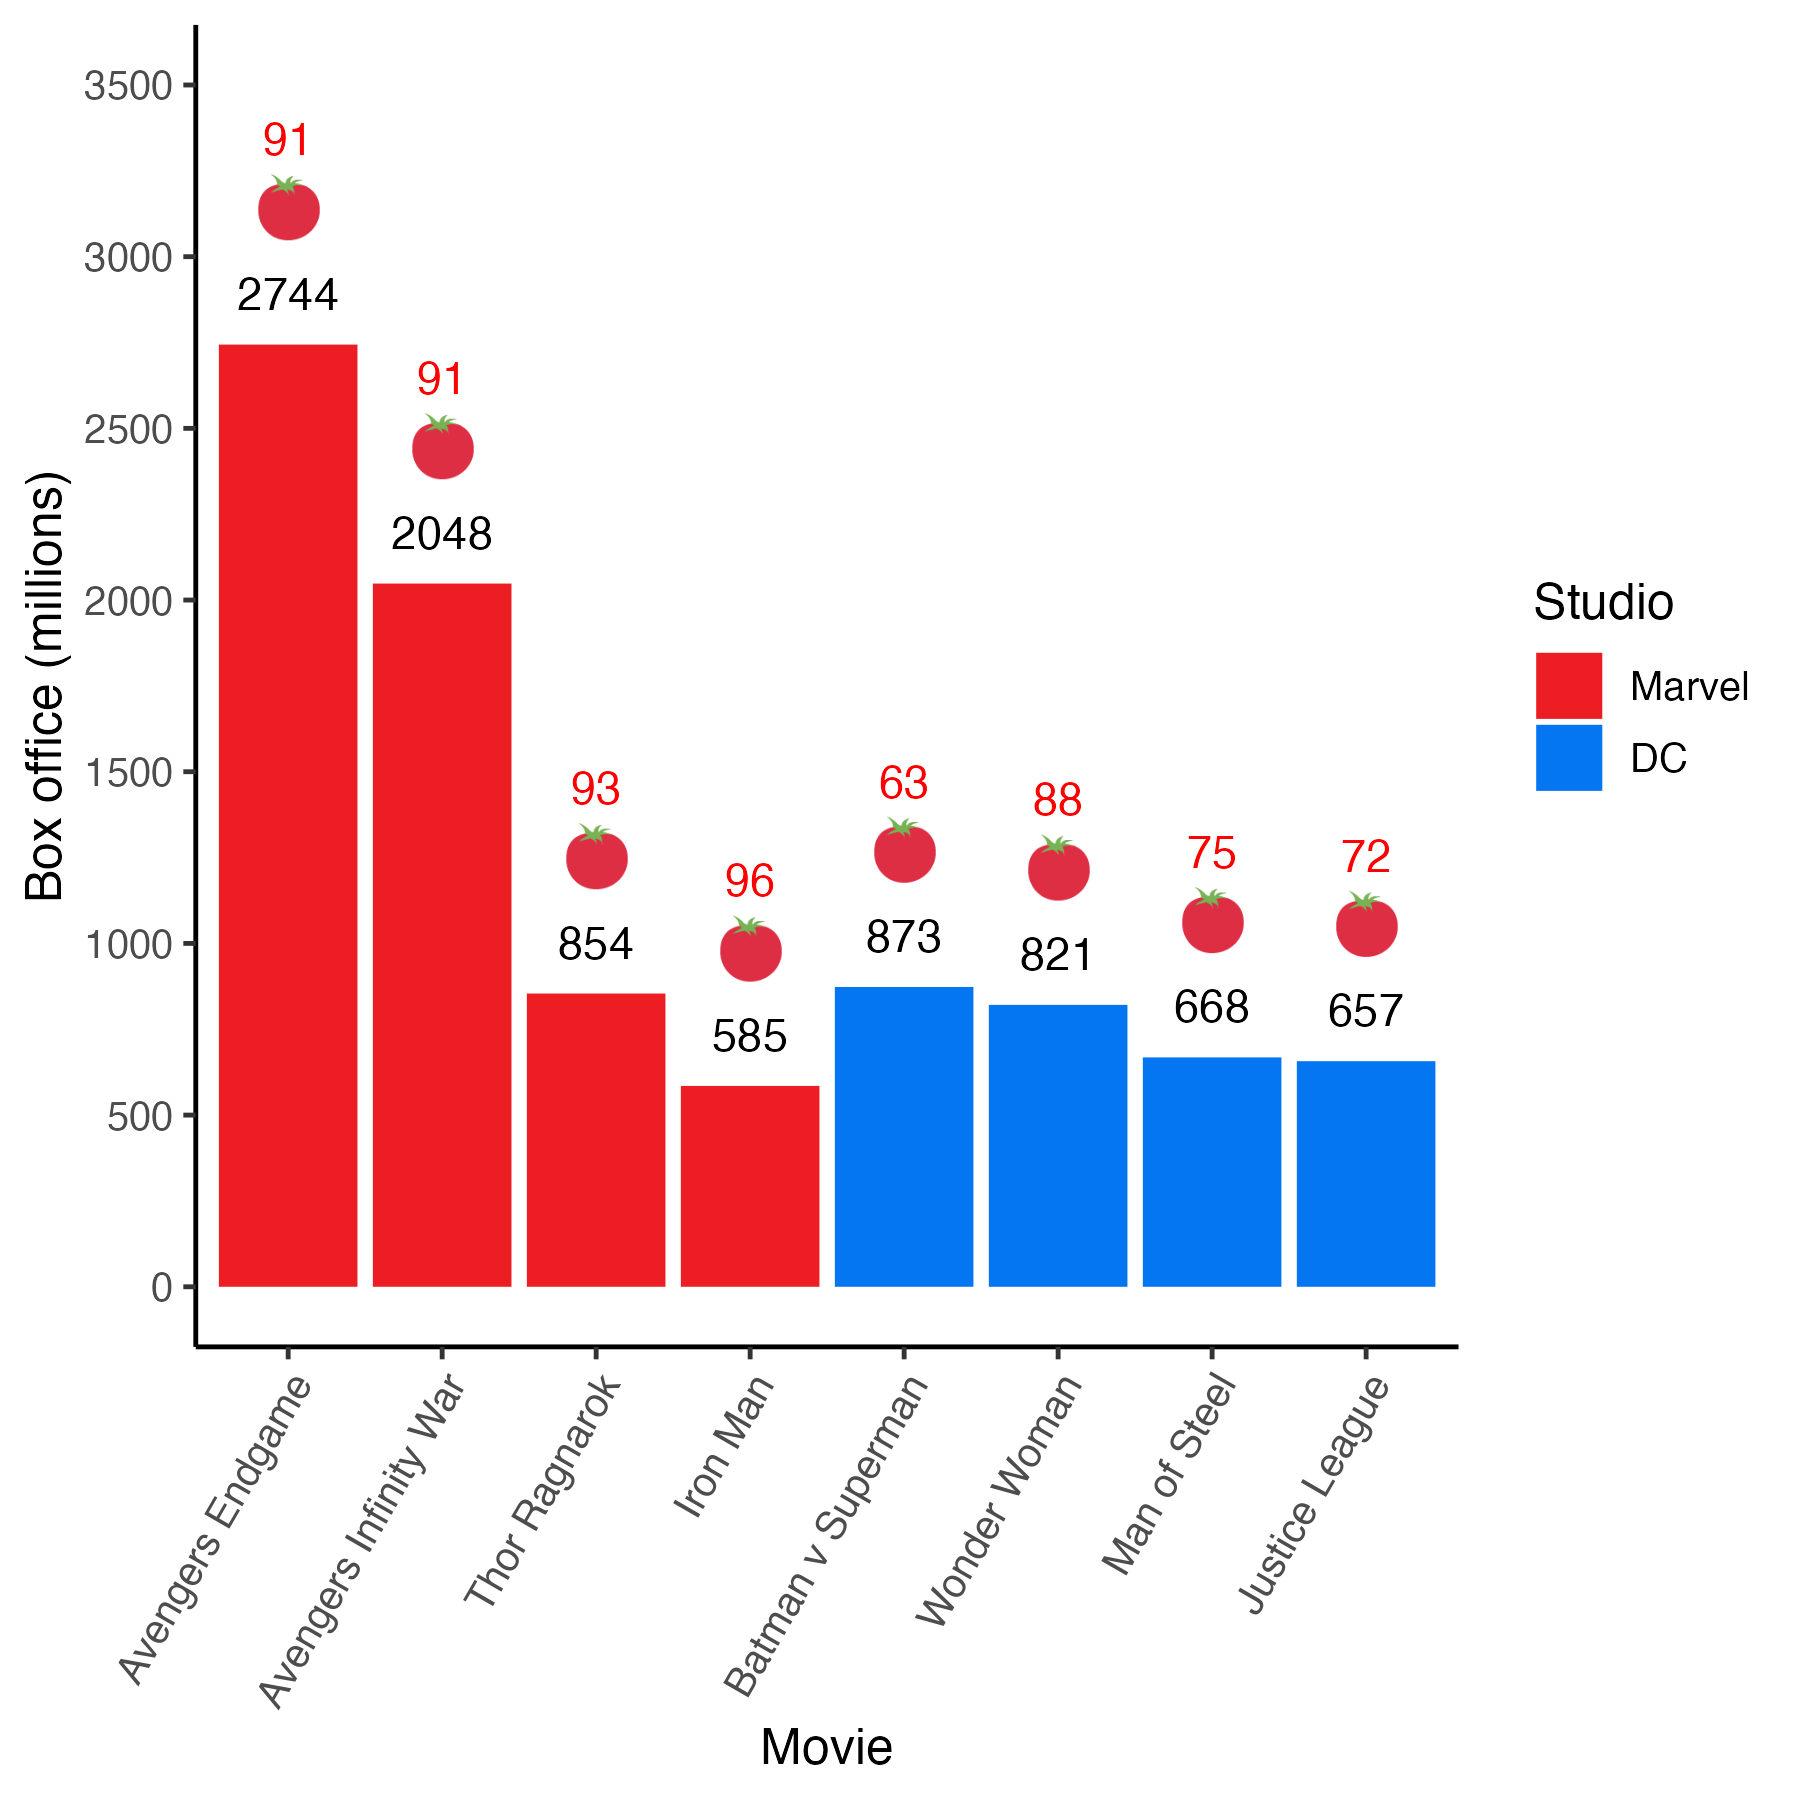
\includegraphics[width=0.65\linewidth]{ch_graphing/images/emoji_graph}

\section{Accessible Colors}\label{accessible-colors}

The current version of the graph is much improved from where we started at the begining of the chapter. One notable improvement was the use of the ``proper'' colors for the Marvel and DC studios. Although using these colors was aethetically pleasing, a major consideration is ensuring your graphs are accessible to a wide audience.

Color blindness is an issue that affects approximately five percent of the population. A nuanced discussion of the different types of color blindness is beyond the scope of this chapter. We can, however, take a moment to think about every graph as being composed of two parts that work together to create the colors overall image. We can think of there being a lightness (i.e., light vs.~dark) component and a hue component (e.g., magenta, yellow, etc.). Together these two components work together to create colors that we see. This distinction between lightness and hue is relevant to all images not just graphs \citep[see][]{margulis2005photoshop}.

\begin{figure}
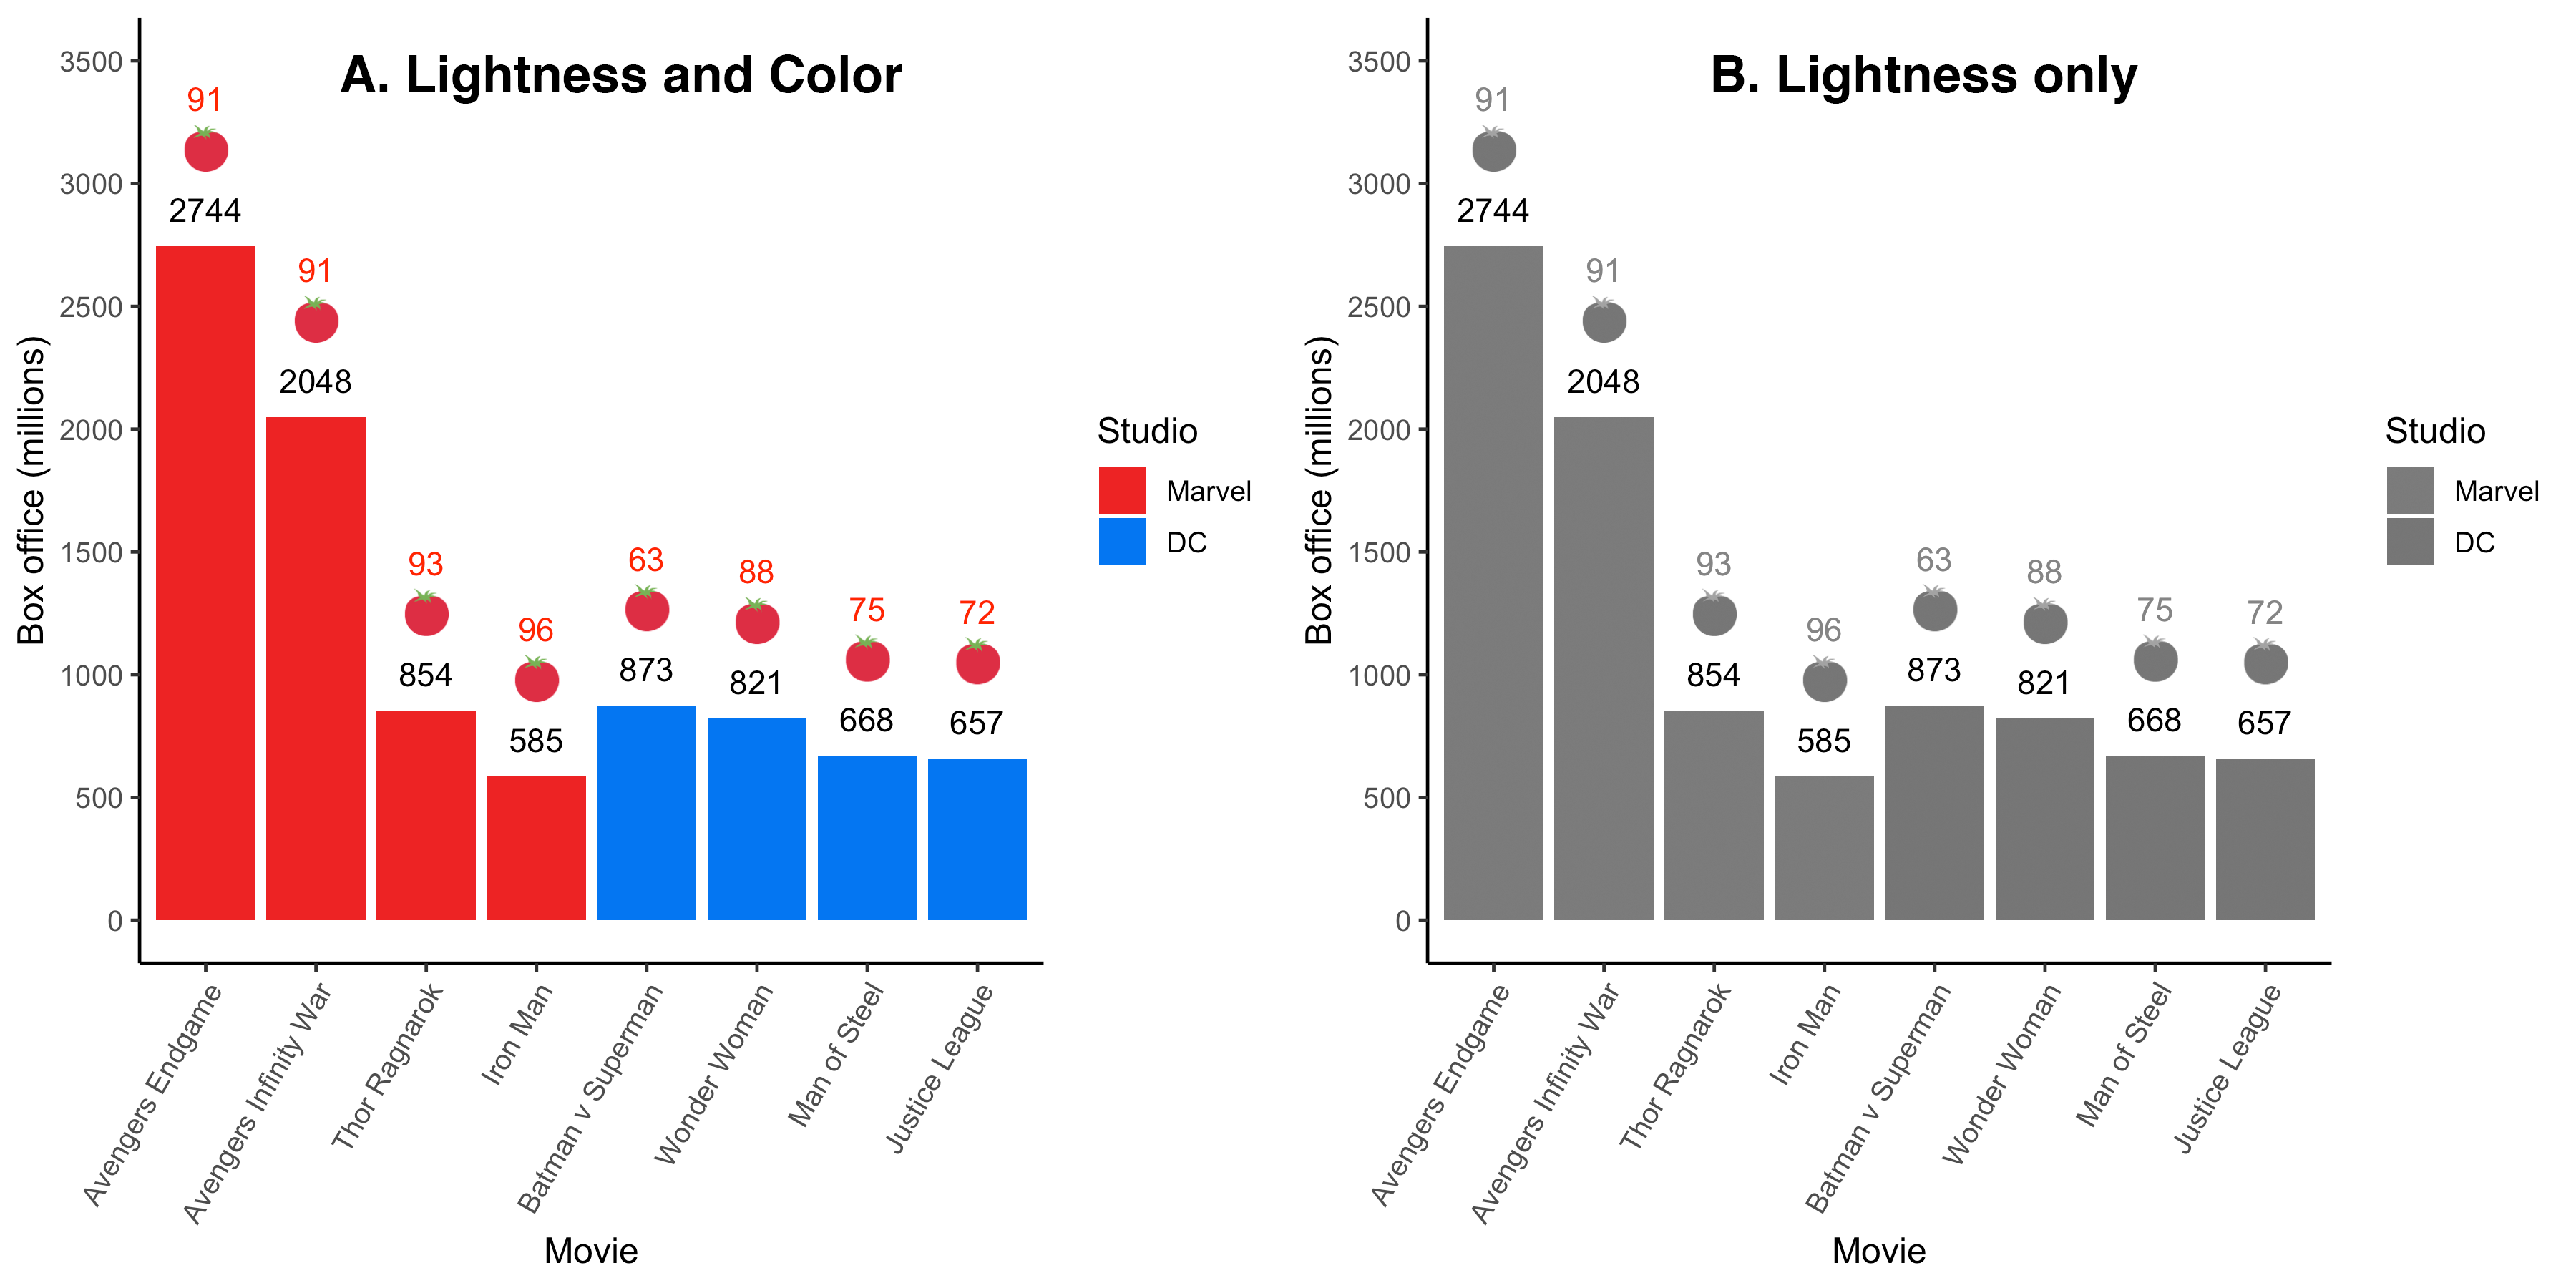
\includegraphics[width=0.75\linewidth]{ch_graphing/images/nocolorcomparison} \caption{Hue removed from current graph}\label{fig:colorcomparison}
\end{figure}

Figure \ref{fig:colorcomparison}A presents our current graph whereas Figure \ref{fig:colorcomparison}B presents the same graph with the hue component removed. You can see that when the hue component is removed that the distinction between the Marvel and DC bars is also removed. The particular colors used to represent Marvel/DC differ in terms of hue but not lightness. Consequently, when we remove the hue component we are left with a graph, \ref{fig:colorcomparison}B, that does not differentiate between the two studios. In order for a color graph to be accessible to people with color blindness we need to pick colors that vary in terms of lightness as well as hue. We can do that with the help of the RColorBrewer package.

\subsection{RColorBrewer}\label{rcolorbrewer}

\subsubsection{Picking a palette}\label{picking-a-palette}

The RColorBrewer package can be used to generate color palettes for graphs that are accessible to people with color blindness. That is, it creates sets of colors, called palettes, for which the colors vary in terms of both lightness and hue. You can see the color-blind accessible palettes, along with their respective names, by using the command below. This code produces a wide range of color-blind accessible palettes with a large number of colors in each palette - as illustrated in Figure \ref{fig:colorpal}.

\begin{Shaded}
\begin{Highlighting}[]
\FunctionTok{library}\NormalTok{(RColorBrewer)}
\FunctionTok{display.brewer.all}\NormalTok{(}\AttributeTok{n =} \ConstantTok{NULL}\NormalTok{, }\AttributeTok{colorblindFriendly =} \ConstantTok{TRUE}\NormalTok{)}
\end{Highlighting}
\end{Shaded}

\begin{figure}
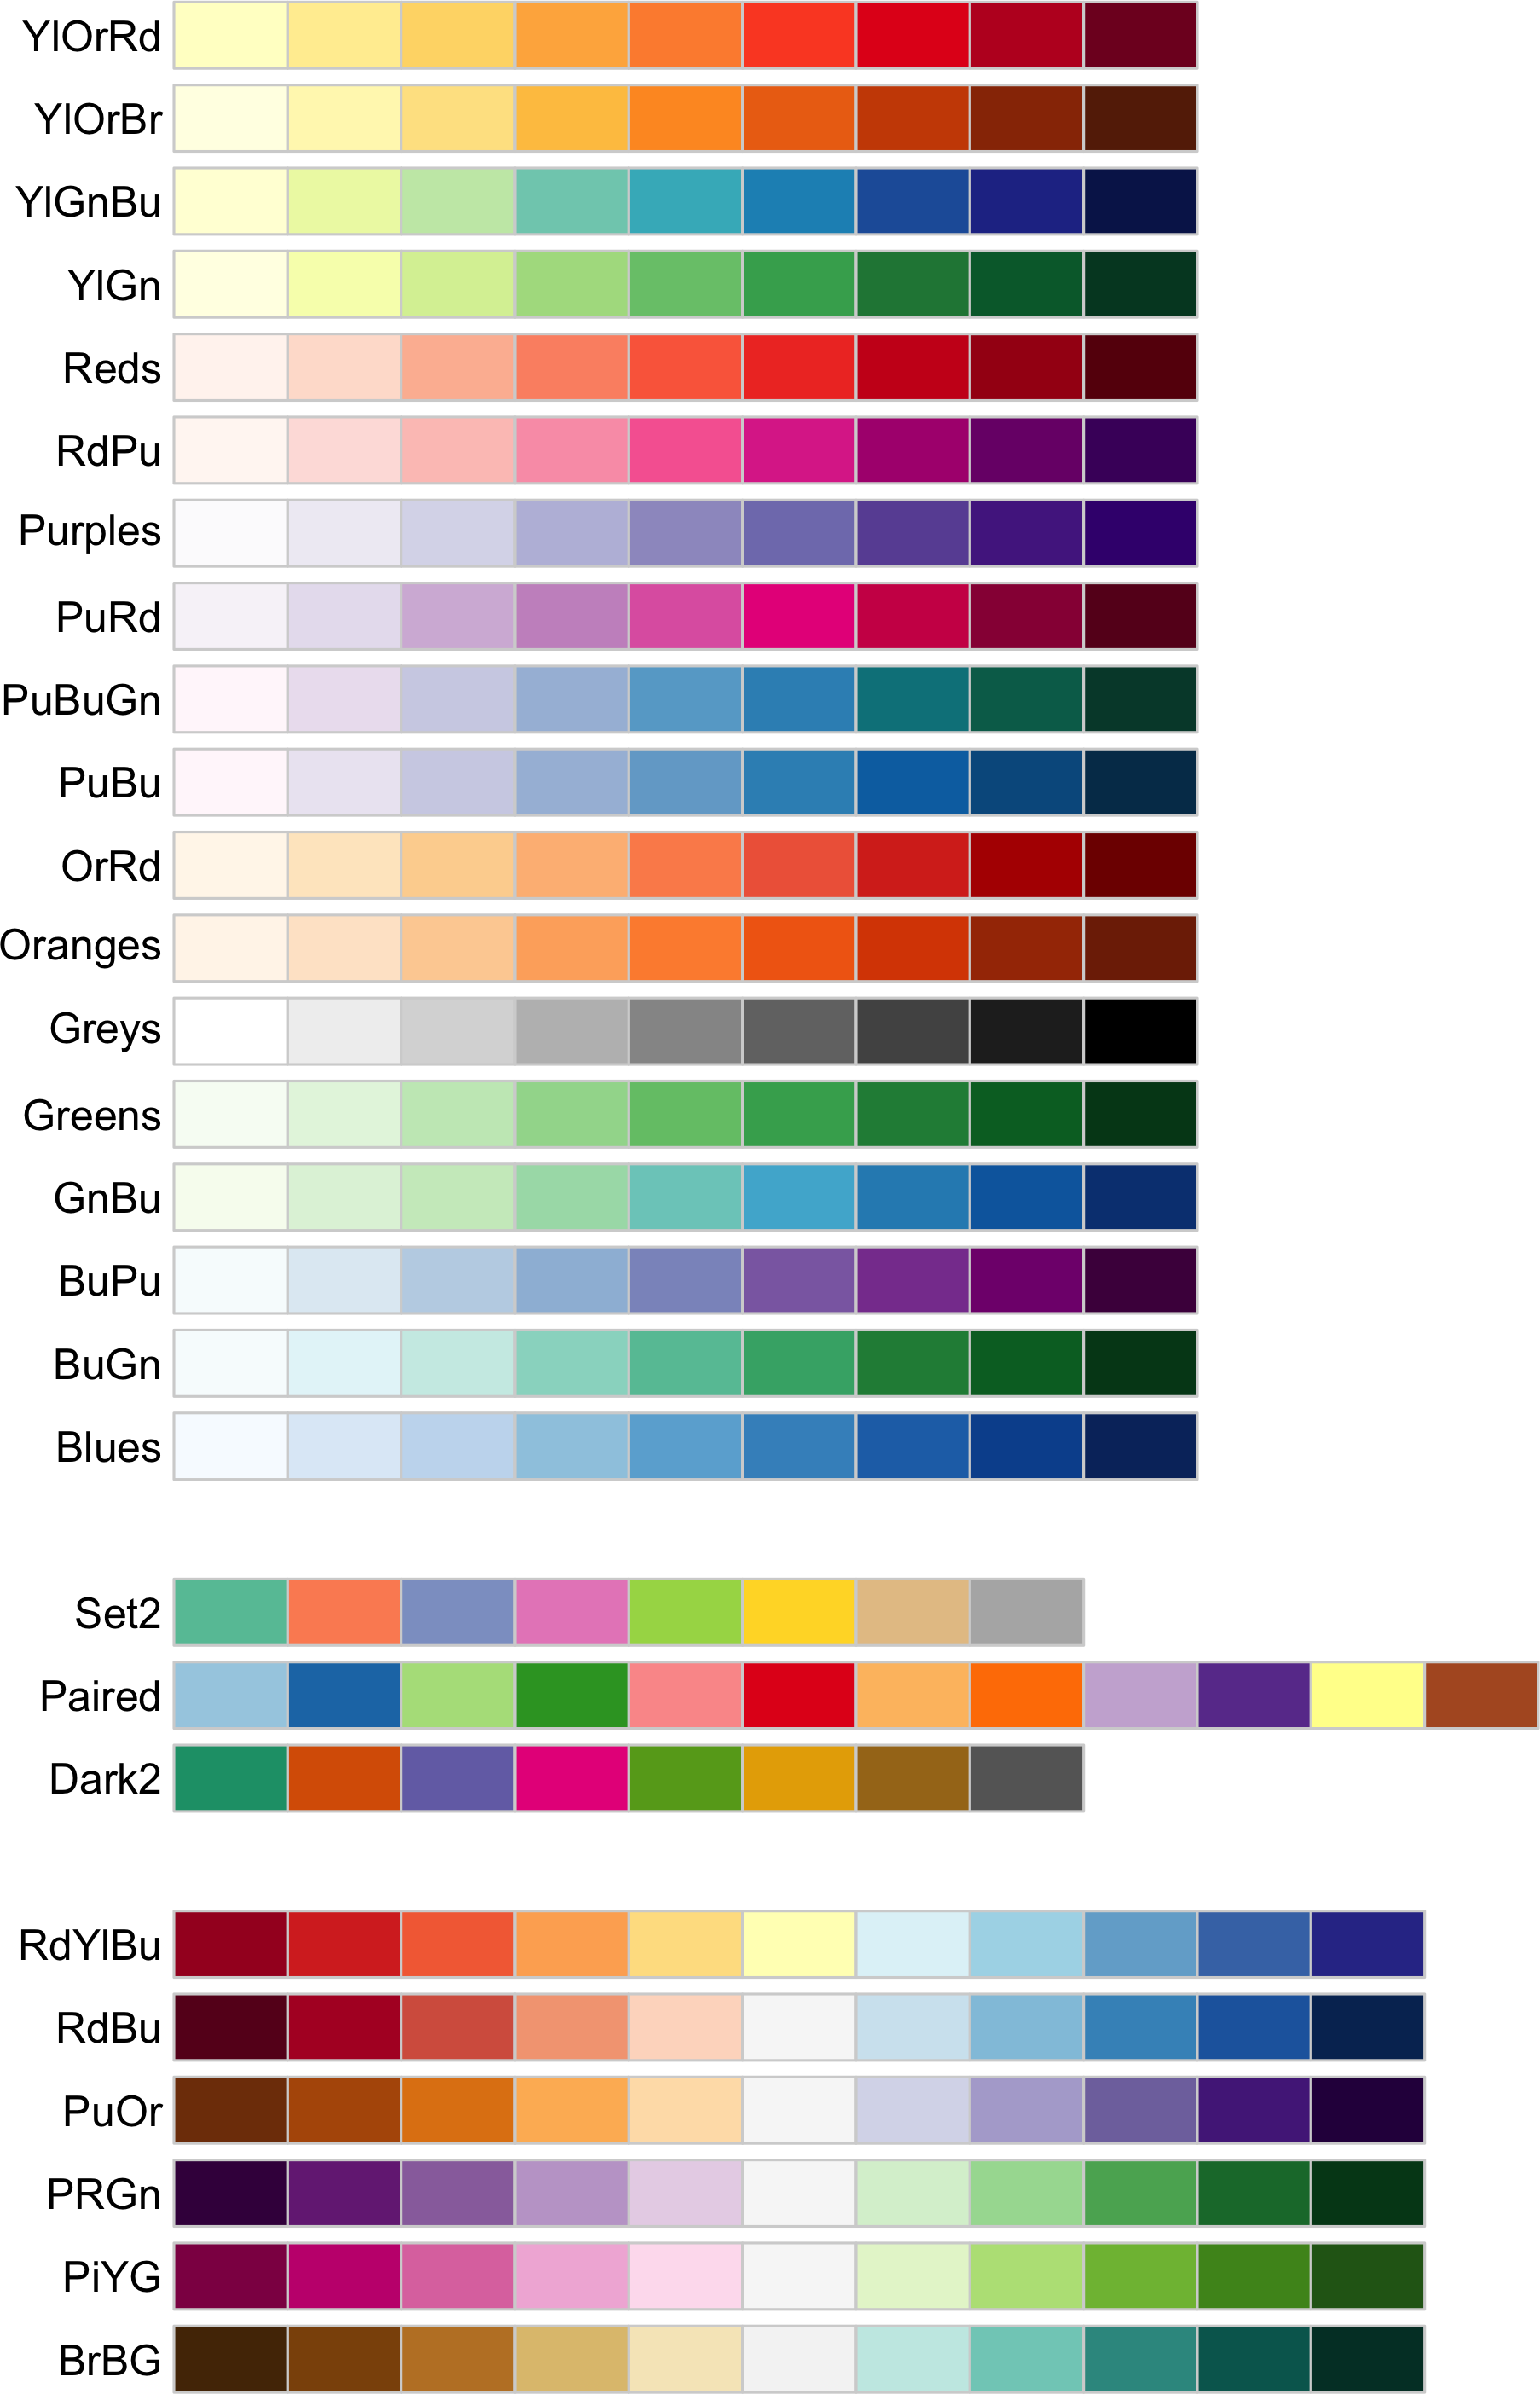
\includegraphics[width=0.7\linewidth,height=0.7\textheight]{ch_graphing/images/colors_all} \caption{Wide range color palette (color-blind accessible)}\label{fig:colorpal}
\end{figure}

\newpage

In Figure \ref{fig:colorpal}, above, we showed palettes with a large number of colors. But if you have a smaller number of possible colors in your graph - you want a palette with fewer colors (to ensure maximum contrast between those colors). You can, for example, obtain palettes with only three colors using the code below.

\begin{Shaded}
\begin{Highlighting}[]
\FunctionTok{library}\NormalTok{(RColorBrewer)}
\FunctionTok{display.brewer.all}\NormalTok{(}\AttributeTok{n =} \DecValTok{3}\NormalTok{, }\AttributeTok{colorblindFriendly =} \ConstantTok{TRUE}\NormalTok{)}
\end{Highlighting}
\end{Shaded}

The above code generates the three-color palettes presented in Figure \ref{fig:colorspalthree}.

\begin{figure}
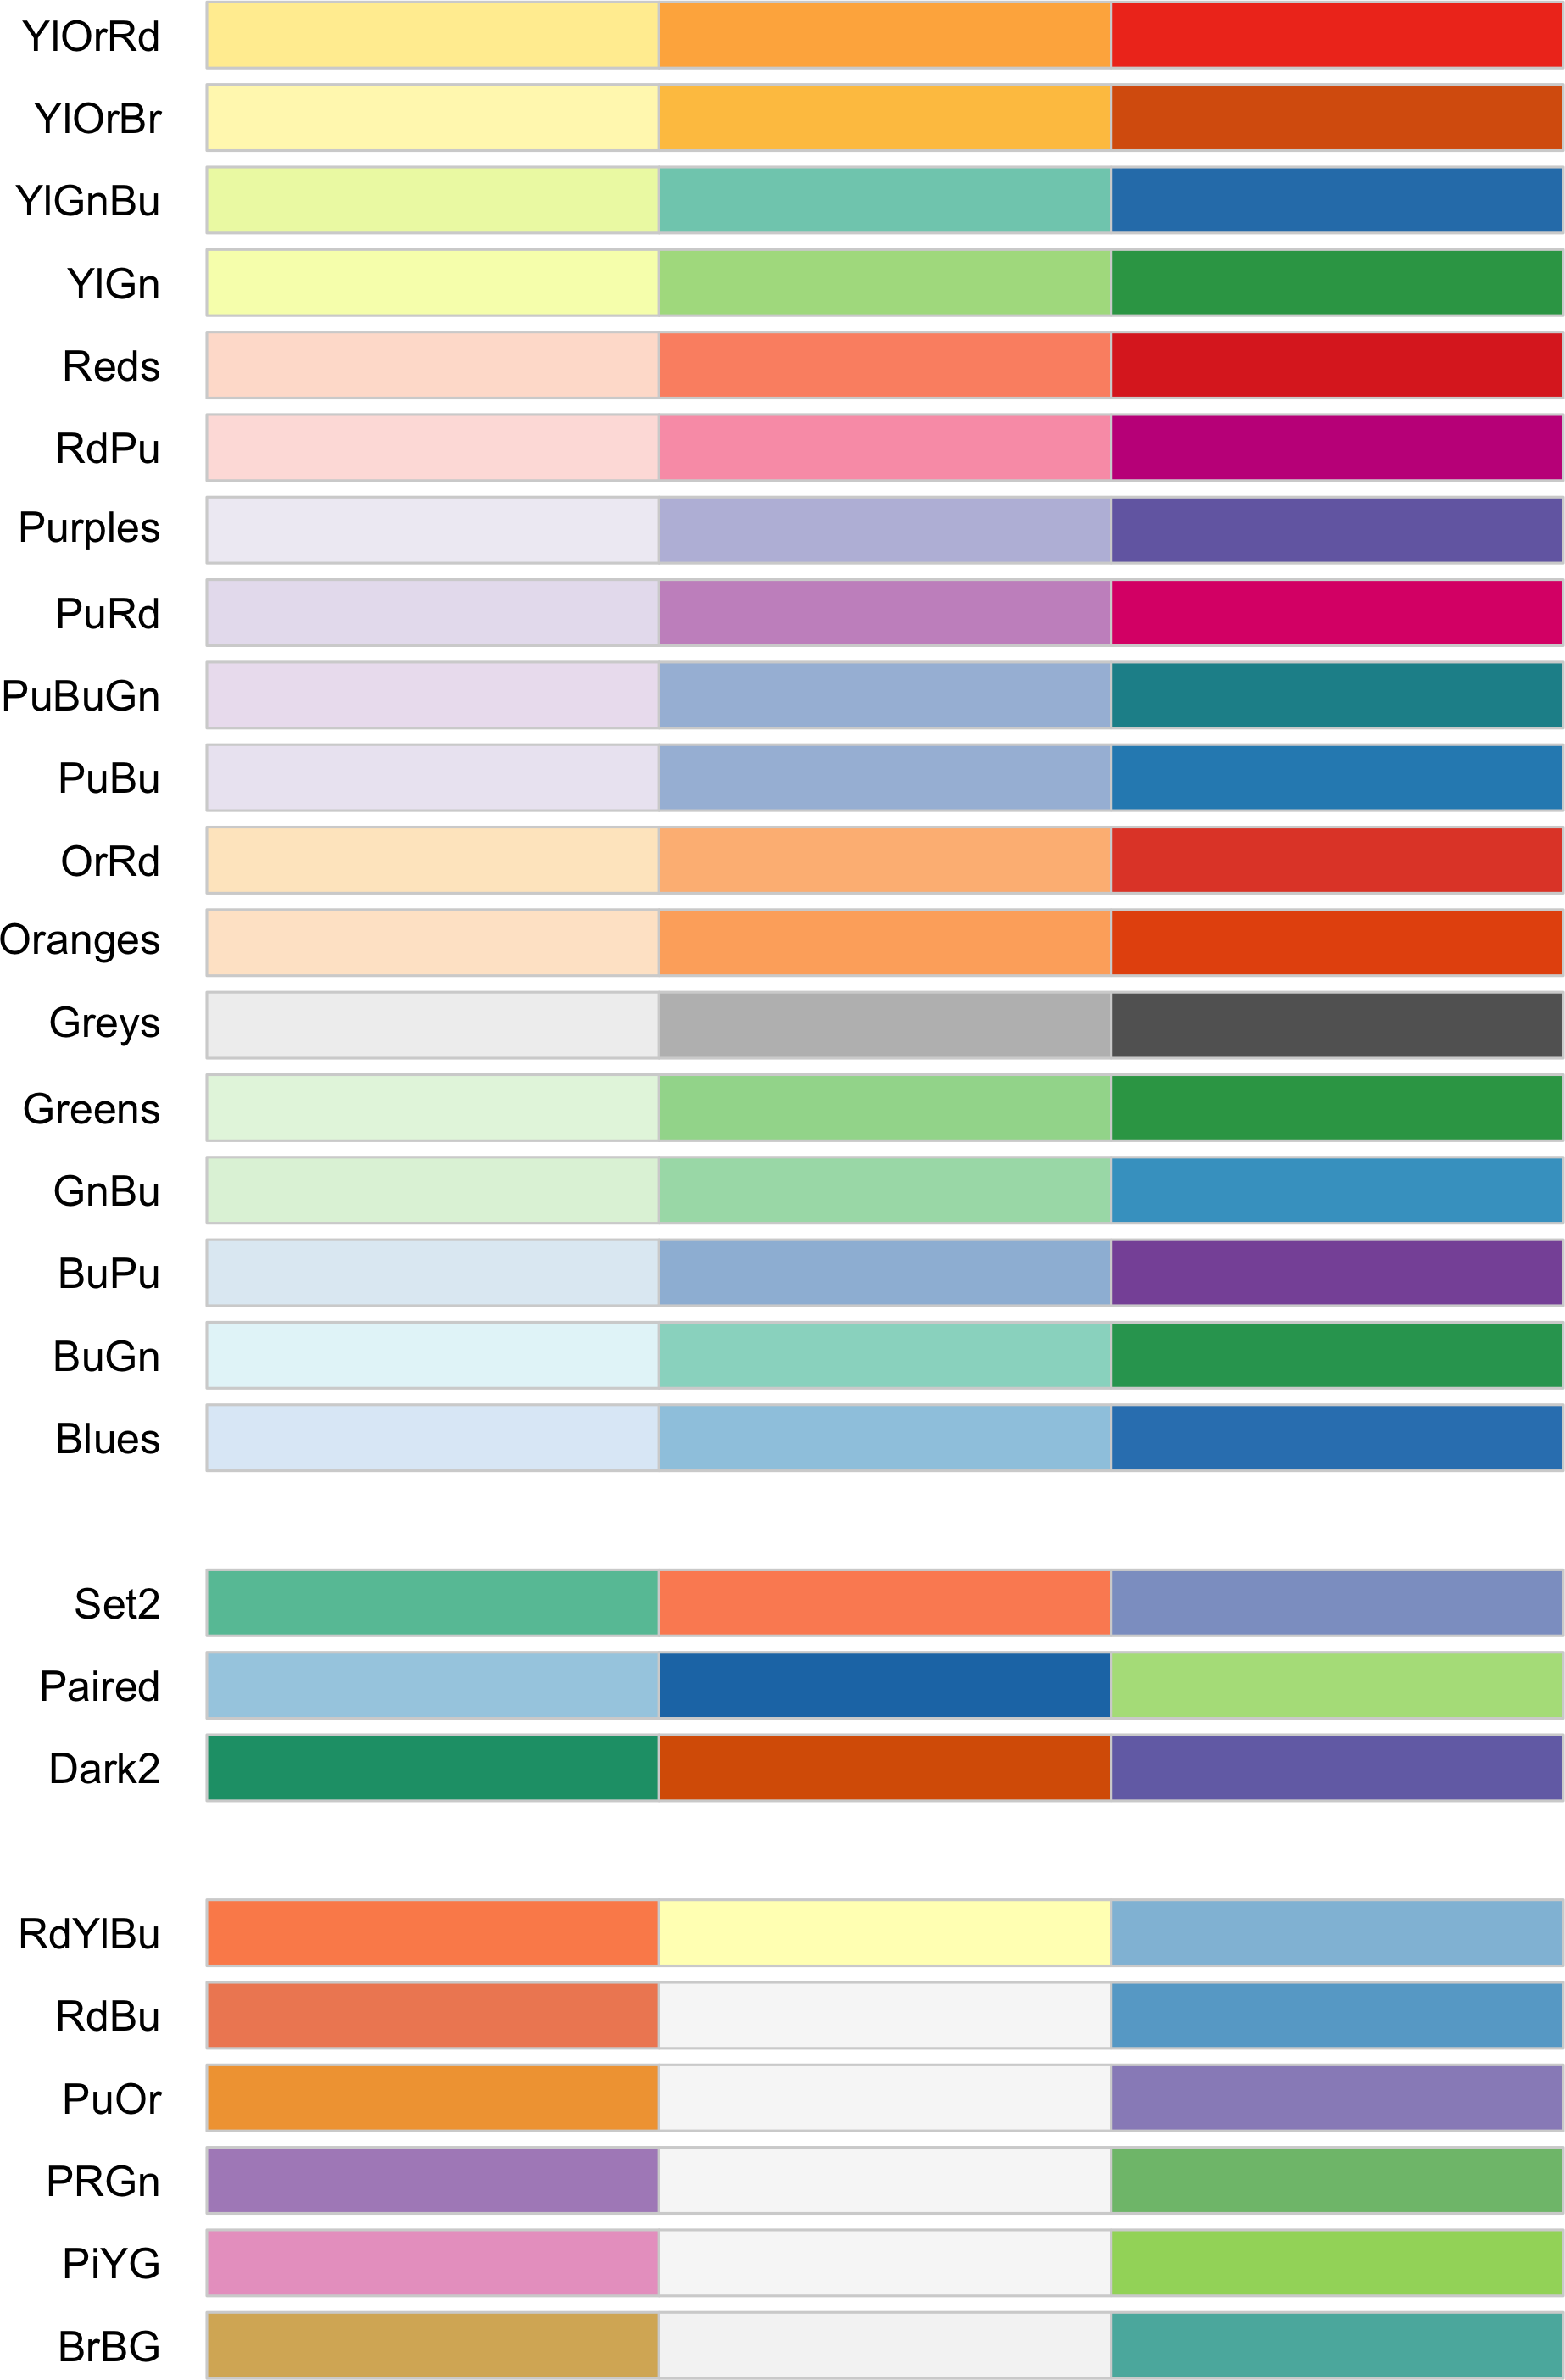
\includegraphics[width=0.7\linewidth,height=0.7\textheight]{ch_graphing/images/colors_3} \caption{Narrow range color palette (color-blind accessible)}\label{fig:colorspalthree}
\end{figure}

\newpage

\subsubsection{Using a palette}\label{using-a-palette}

We can use a color palette by specifying its name within scale\_fill\_brewer(). We want to use the ``Paired'' palette in Figure \ref{fig:colorspalthree} so we use the code: scale\_fill\_brewer(palette = ``Paired''), as illustrated below:

\begin{Shaded}
\begin{Highlighting}[]
\NormalTok{my\_graph }\OtherTok{\textless{}{-}} \FunctionTok{ggplot}\NormalTok{(}\AttributeTok{data =}\NormalTok{ movie\_data,}
           \AttributeTok{mapping =} \FunctionTok{aes}\NormalTok{(}\AttributeTok{x =}\NormalTok{ title,}
                         \AttributeTok{y =}\NormalTok{ boxoffice,}
                         \AttributeTok{label =}\NormalTok{ boxoffice, }
                         \AttributeTok{fill =}\NormalTok{ studio)) }\SpecialCharTok{+}
  \FunctionTok{geom\_col}\NormalTok{() }\SpecialCharTok{+}
  \FunctionTok{geom\_text}\NormalTok{(}\AttributeTok{nudge\_y =} \DecValTok{150}\NormalTok{)  }\SpecialCharTok{+}
  \FunctionTok{geom\_text}\NormalTok{(}\AttributeTok{mapping =} \FunctionTok{aes}\NormalTok{(}\AttributeTok{label =}\NormalTok{ tomatoes\_aud), }
            \AttributeTok{nudge\_y =} \DecValTok{600}\NormalTok{, }
            \AttributeTok{colour =} \StringTok{"red"}\NormalTok{) }\SpecialCharTok{+}
  \FunctionTok{geom\_emoji}\NormalTok{(}\AttributeTok{mapping =} \FunctionTok{aes}\NormalTok{(}\AttributeTok{y =}\NormalTok{ boxoffice }\SpecialCharTok{+} \DecValTok{400}\NormalTok{),}
             \AttributeTok{emoji=}\StringTok{"1f345"}\NormalTok{) }\SpecialCharTok{+}
  \FunctionTok{coord\_cartesian}\NormalTok{(}\AttributeTok{ylim =} \FunctionTok{c}\NormalTok{(}\DecValTok{0}\NormalTok{, }\DecValTok{3500}\NormalTok{)) }\SpecialCharTok{+}
  \FunctionTok{scale\_y\_continuous}\NormalTok{(}\AttributeTok{breaks =} \FunctionTok{seq}\NormalTok{(}\DecValTok{0}\NormalTok{, }\DecValTok{3500}\NormalTok{, }\AttributeTok{by =} \DecValTok{500}\NormalTok{)) }\SpecialCharTok{+}
  \FunctionTok{labs}\NormalTok{(}\AttributeTok{x =} \StringTok{"Movie"}\NormalTok{,}
       \AttributeTok{y =} \StringTok{"Box office (millions)"}\NormalTok{,}
       \AttributeTok{fill =} \StringTok{"Studio"}\NormalTok{) }\SpecialCharTok{+}
  \FunctionTok{theme\_classic}\NormalTok{(}\DecValTok{12}\NormalTok{) }\SpecialCharTok{+}
  \FunctionTok{theme}\NormalTok{(}\AttributeTok{axis.text.x =} \FunctionTok{element\_text}\NormalTok{(}\AttributeTok{angle =} \DecValTok{60}\NormalTok{, }
                                   \AttributeTok{hjust =} \DecValTok{1}\NormalTok{)) }\SpecialCharTok{+}
  \FunctionTok{scale\_fill\_brewer}\NormalTok{(}\AttributeTok{palette =} \StringTok{"Paired"}\NormalTok{)}
\end{Highlighting}
\end{Shaded}

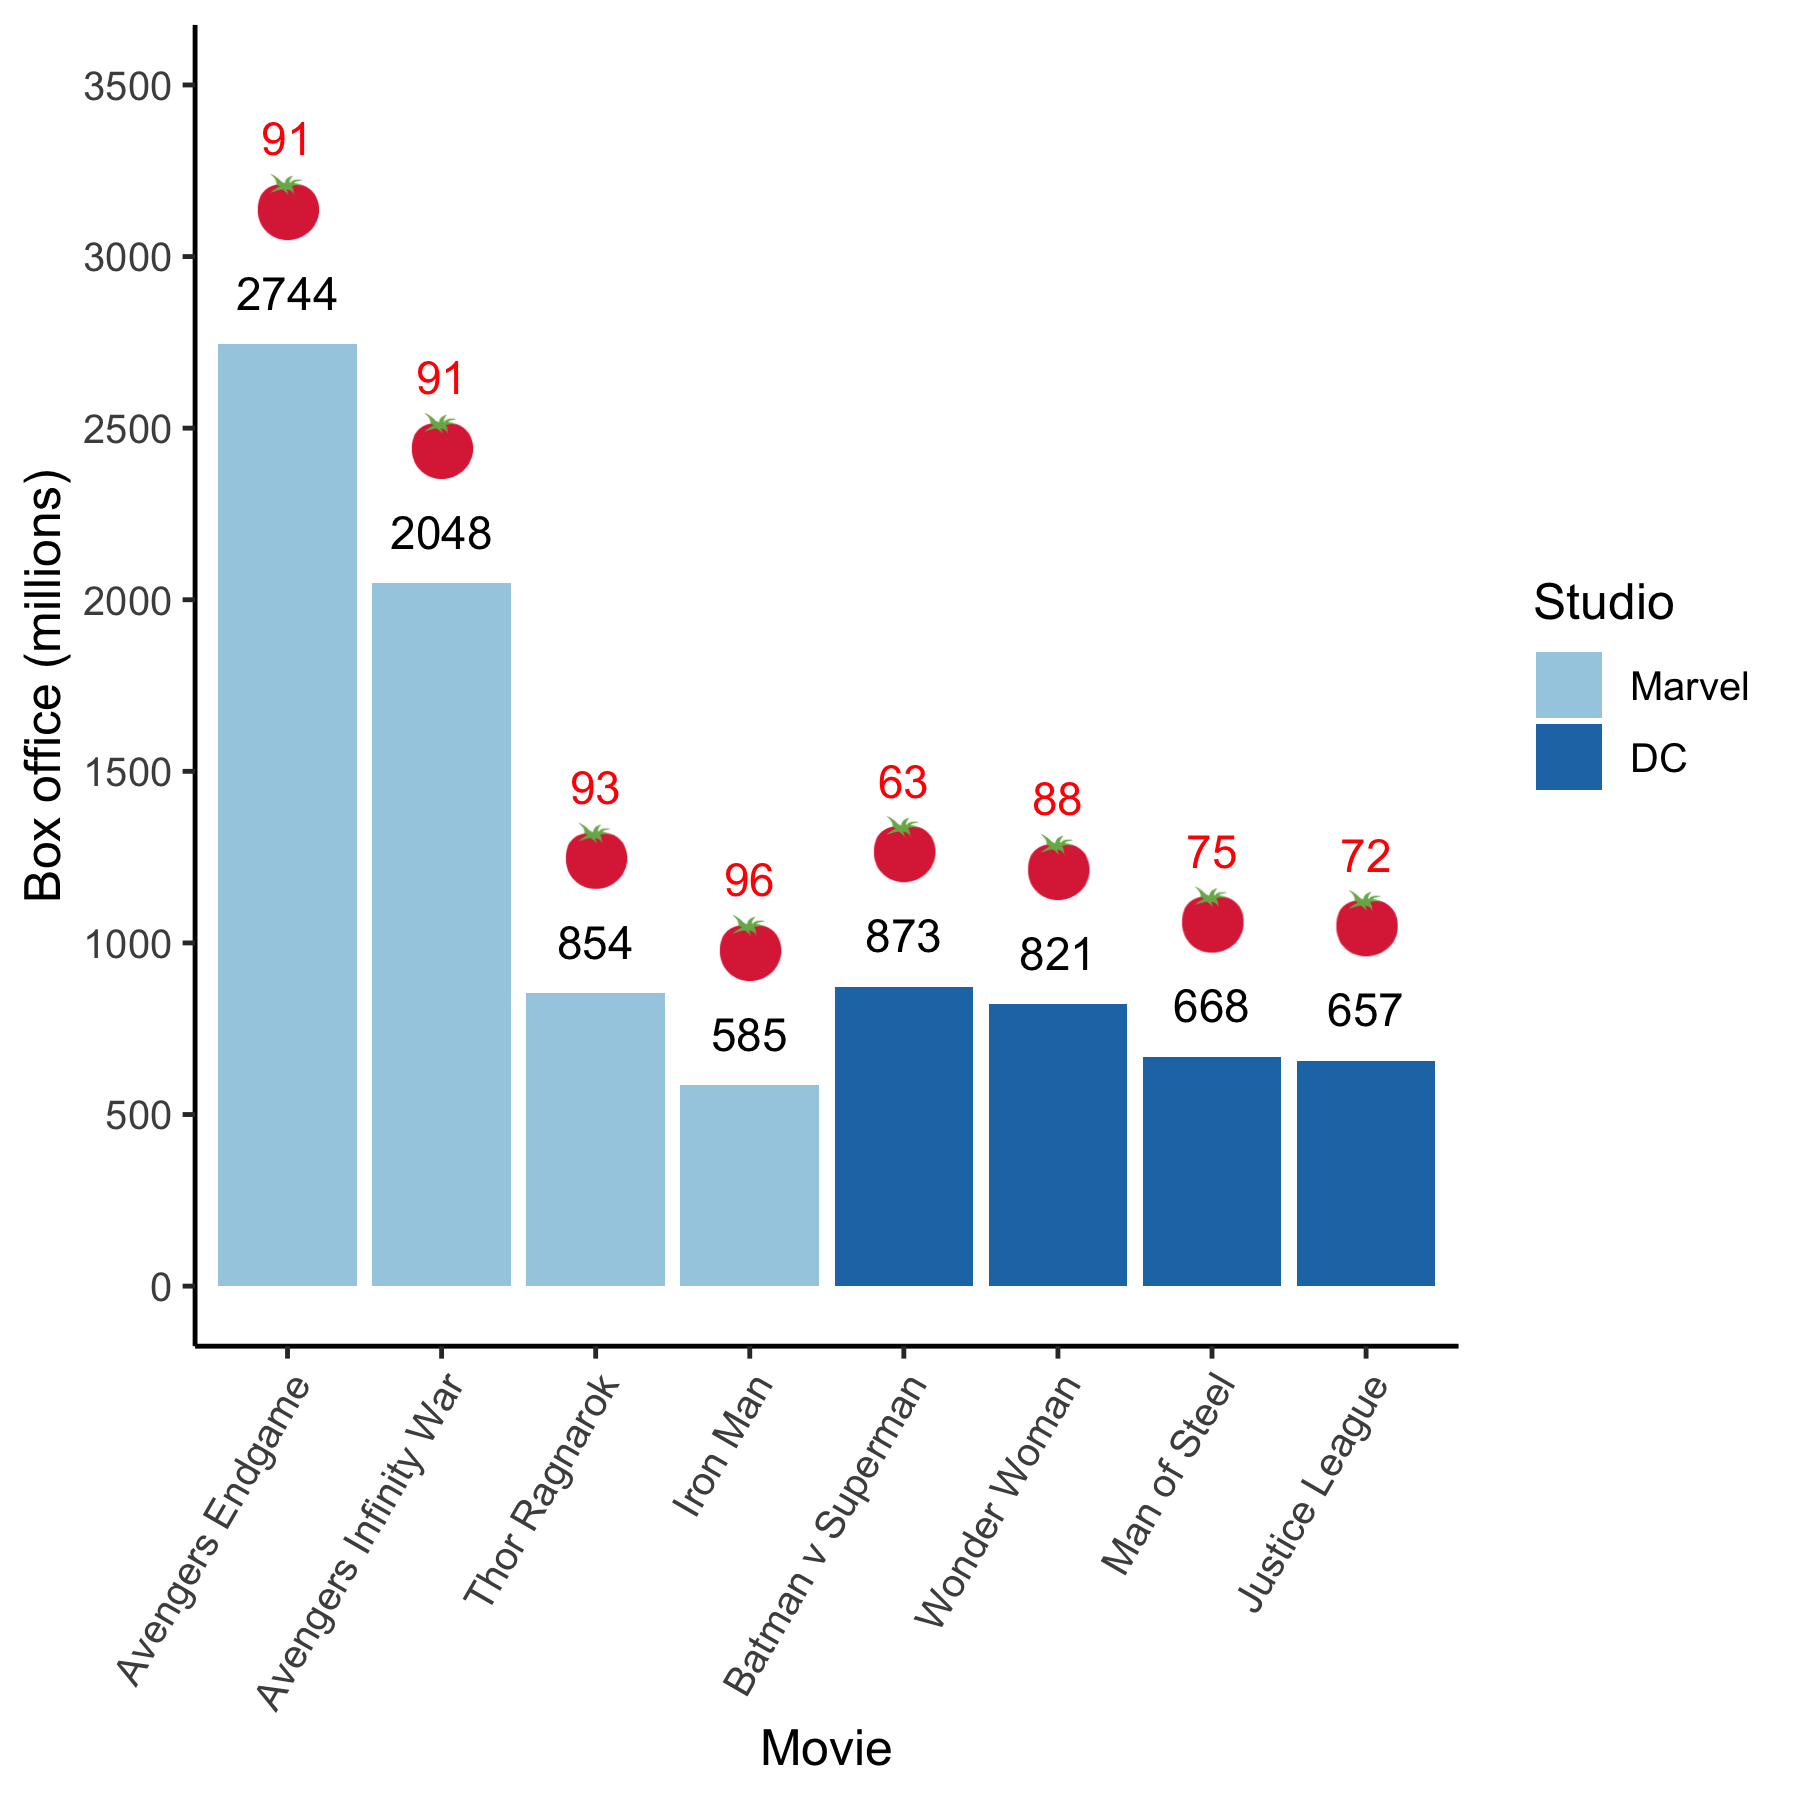
\includegraphics[width=0.65\linewidth]{ch_graphing/images/emoji_graph4}

\subsubsection{Palette subsets}\label{palette-subsets}

Our graph had only two colors but the ``Paired'' palette had three colors. When ggplot made the graph it automatically used the first two colors of the three color palette. What if you wanted the second two colors in the palette? We can do that but we have to revert to a manual color process like we used before via the scale\_fill\_manual(). But we want to do so using the colors from the ``Paired'' palette. We can obtain the color codes for the ``Paired'' palette with the code below:

\begin{Shaded}
\begin{Highlighting}[]
\FunctionTok{brewer.pal}\NormalTok{(}\AttributeTok{n =} \DecValTok{3}\NormalTok{, }\AttributeTok{name =} \StringTok{"Paired"}\NormalTok{)}
\end{Highlighting}
\end{Shaded}

\begin{verbatim}
## [1] "#A6CEE3" "#1F78B4" "#B2DF8A"
\end{verbatim}

The numbers in the output correspond to values representing the three colors of the ``Paired'' palette, see Figure \ref{fig:pairedpal}. If we want the last two colors in the palette for our graph that means we want the colors: \#1F78B4 and \#B2DF8A.

\begin{figure}
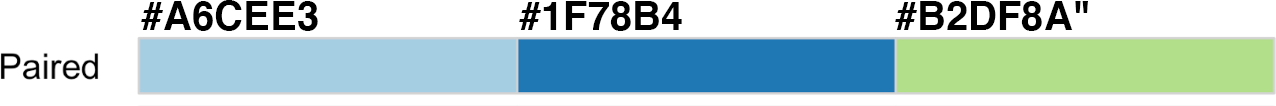
\includegraphics[width=0.75\linewidth]{ch_graphing/images/pairedpalette} \caption{Paired palette colors with hex numbers}\label{fig:pairedpal}
\end{figure}

We can put the two colors we want (\#1F78B4 and \#B2DF8A) on the graph by using the scale\_fill\_manual() command - instead of the scale\_fill\_brewer() command. We can see this in the code below:

\begin{Shaded}
\begin{Highlighting}[]
\NormalTok{my\_graph }\OtherTok{\textless{}{-}} \FunctionTok{ggplot}\NormalTok{(}\AttributeTok{data =}\NormalTok{ movie\_data,}
           \AttributeTok{mapping =} \FunctionTok{aes}\NormalTok{(}\AttributeTok{x =}\NormalTok{ title,}
                         \AttributeTok{y =}\NormalTok{ boxoffice,}
                         \AttributeTok{label =}\NormalTok{ boxoffice, }
                         \AttributeTok{fill =}\NormalTok{ studio)) }\SpecialCharTok{+}
  \FunctionTok{geom\_col}\NormalTok{() }\SpecialCharTok{+}
  \FunctionTok{geom\_text}\NormalTok{(}\AttributeTok{nudge\_y =} \DecValTok{150}\NormalTok{)  }\SpecialCharTok{+}
  \FunctionTok{geom\_text}\NormalTok{(}\AttributeTok{mapping =} \FunctionTok{aes}\NormalTok{(}\AttributeTok{label =}\NormalTok{ tomatoes\_aud), }
            \AttributeTok{nudge\_y =} \DecValTok{600}\NormalTok{, }
            \AttributeTok{colour =} \StringTok{"red"}\NormalTok{) }\SpecialCharTok{+}
  \FunctionTok{geom\_emoji}\NormalTok{(}\AttributeTok{mapping =} \FunctionTok{aes}\NormalTok{(}\AttributeTok{y =}\NormalTok{ boxoffice }\SpecialCharTok{+} \DecValTok{400}\NormalTok{),}
             \AttributeTok{emoji=}\StringTok{"1f345"}\NormalTok{) }\SpecialCharTok{+}
  \FunctionTok{coord\_cartesian}\NormalTok{(}\AttributeTok{ylim =} \FunctionTok{c}\NormalTok{(}\DecValTok{0}\NormalTok{, }\DecValTok{3500}\NormalTok{)) }\SpecialCharTok{+}
  \FunctionTok{scale\_y\_continuous}\NormalTok{(}\AttributeTok{breaks =} \FunctionTok{seq}\NormalTok{(}\DecValTok{0}\NormalTok{, }\DecValTok{3500}\NormalTok{, }\AttributeTok{by =} \DecValTok{500}\NormalTok{)) }\SpecialCharTok{+}
  \FunctionTok{labs}\NormalTok{(}\AttributeTok{x =} \StringTok{"Movie"}\NormalTok{,}
       \AttributeTok{y =} \StringTok{"Box office (millions)"}\NormalTok{,}
       \AttributeTok{fill =} \StringTok{"Studio"}\NormalTok{) }\SpecialCharTok{+}
  \FunctionTok{theme\_classic}\NormalTok{(}\DecValTok{12}\NormalTok{) }\SpecialCharTok{+}
  \FunctionTok{theme}\NormalTok{(}\AttributeTok{axis.text.x =} \FunctionTok{element\_text}\NormalTok{(}\AttributeTok{angle =} \DecValTok{60}\NormalTok{, }
                                   \AttributeTok{hjust =} \DecValTok{1}\NormalTok{)) }\SpecialCharTok{+}
  \FunctionTok{scale\_fill\_manual}\NormalTok{(}\AttributeTok{values =} \FunctionTok{c}\NormalTok{(}\StringTok{"\#1F78B4"}\NormalTok{, }\StringTok{"\#B2DF8A"}\NormalTok{))}
\end{Highlighting}
\end{Shaded}

\includegraphics[width=0.65\linewidth]{ch_graphing/images/emoji_graph5}

Now that we have used a color-blind accessible palette in the graph we can look at the graph without the hue component. In Figure \ref{fig:colorcomparison2}B, below, notice that the bars representing the two studios are easily distinguishable based on lightness alone. That is, the lightness graph in Figure \ref{fig:colorcomparison2}B demonstrates the new color-blind accessible colors vary in term of both hue and lightness - not just hue. Therefore, when hue is removed the two colors are distinguishable. This makes the graph accessible to color-blind individuals.

\begin{figure}
\includegraphics[width=0.75\linewidth]{ch_graphing/images/nocolorcomparison2} \caption{Color information (i.e., hue) removed from new color-blind accessible graph}\label{fig:colorcomparison2}
\end{figure}

\subsection{Avoid color}\label{avoid-color}

When you only have two colors on a graph another option for creating an accessible graph is to remove the colors entirely and make a black and white graph. In the code below we use scale\_fill\_manual() with the values ``\#ffffff'' (white) and ``\,``\#000000'' (black). The intent was to create bars that are white for Marvel and black for DC. Unfortunately, because the graph has a white background you can see this resulted in the Marvel bars disappearing.

\begin{Shaded}
\begin{Highlighting}[]
\NormalTok{my\_graph }\OtherTok{\textless{}{-}} \FunctionTok{ggplot}\NormalTok{(}\AttributeTok{data =}\NormalTok{ movie\_data,}
           \AttributeTok{mapping =} \FunctionTok{aes}\NormalTok{(}\AttributeTok{x =}\NormalTok{ title,}
                         \AttributeTok{y =}\NormalTok{ boxoffice,}
                         \AttributeTok{label =}\NormalTok{ boxoffice, }
                         \AttributeTok{fill =}\NormalTok{ studio)) }\SpecialCharTok{+}
  \FunctionTok{geom\_col}\NormalTok{() }\SpecialCharTok{+}
  \FunctionTok{geom\_text}\NormalTok{(}\AttributeTok{nudge\_y =} \DecValTok{150}\NormalTok{)  }\SpecialCharTok{+}
  \FunctionTok{geom\_text}\NormalTok{(}\AttributeTok{mapping =} \FunctionTok{aes}\NormalTok{(}\AttributeTok{label =}\NormalTok{ tomatoes\_aud), }
            \AttributeTok{nudge\_y =} \DecValTok{600}\NormalTok{, }
            \AttributeTok{colour =} \StringTok{"red"}\NormalTok{) }\SpecialCharTok{+}
  \FunctionTok{geom\_emoji}\NormalTok{(}\AttributeTok{mapping =} \FunctionTok{aes}\NormalTok{(}\AttributeTok{y =}\NormalTok{ boxoffice }\SpecialCharTok{+} \DecValTok{400}\NormalTok{),}
             \AttributeTok{emoji=}\StringTok{"1f345"}\NormalTok{) }\SpecialCharTok{+}
  \FunctionTok{coord\_cartesian}\NormalTok{(}\AttributeTok{ylim =} \FunctionTok{c}\NormalTok{(}\DecValTok{0}\NormalTok{, }\DecValTok{3500}\NormalTok{)) }\SpecialCharTok{+}
  \FunctionTok{scale\_y\_continuous}\NormalTok{(}\AttributeTok{breaks =} \FunctionTok{seq}\NormalTok{(}\DecValTok{0}\NormalTok{, }\DecValTok{3500}\NormalTok{, }\AttributeTok{by =} \DecValTok{500}\NormalTok{)) }\SpecialCharTok{+}
  \FunctionTok{labs}\NormalTok{(}\AttributeTok{x =} \StringTok{"Movie"}\NormalTok{,}
       \AttributeTok{y =} \StringTok{"Box office (millions)"}\NormalTok{,}
       \AttributeTok{fill =} \StringTok{"Studio"}\NormalTok{) }\SpecialCharTok{+}
  \FunctionTok{theme\_classic}\NormalTok{(}\DecValTok{12}\NormalTok{) }\SpecialCharTok{+}
  \FunctionTok{theme}\NormalTok{(}\AttributeTok{axis.text.x =} \FunctionTok{element\_text}\NormalTok{(}\AttributeTok{angle =} \DecValTok{60}\NormalTok{, }
                                   \AttributeTok{hjust =} \DecValTok{1}\NormalTok{)) }\SpecialCharTok{+}
  \FunctionTok{scale\_fill\_manual}\NormalTok{(}\AttributeTok{values =} \FunctionTok{c}\NormalTok{(}\StringTok{"\#ffffff"}\NormalTok{, }\StringTok{"\#000000"}\NormalTok{))}
\end{Highlighting}
\end{Shaded}

\includegraphics[width=0.65\linewidth]{ch_graphing/images/emoji_graph2}

How do we get around the Marvel bars disappearing when we use white?

\textbf{Color vs.~fill.} The ggplot packages makes a distinction between \textbf{fill} and \textbf{color}. The term \textbf{fill} is used to refer to the inside color of bars. In contrast, \textbf{color} is used to the refer to the lines that outline the shape of each bar. In the previous code we used fill to change the colors of the bars but we did not use the ``color'' argument in a command. In the code below, we modify the geom\_col() command to use the ``color'' argument. Specifically, we change geom\_col() to geom\_col(color = ``black''). This change adds a black outline around all the bars -- including the ones with a white fill. You can see the result is a much improved graph. This black/white graph is accessible to everyone.

\begin{Shaded}
\begin{Highlighting}[]
\NormalTok{my\_graph }\OtherTok{\textless{}{-}} \FunctionTok{ggplot}\NormalTok{(}\AttributeTok{data =}\NormalTok{ movie\_data,}
           \AttributeTok{mapping =} \FunctionTok{aes}\NormalTok{(}\AttributeTok{x =}\NormalTok{ title,}
                         \AttributeTok{y =}\NormalTok{ boxoffice,}
                         \AttributeTok{label =}\NormalTok{ boxoffice, }
                         \AttributeTok{fill =}\NormalTok{ studio)) }\SpecialCharTok{+}
  \FunctionTok{geom\_col}\NormalTok{(}\AttributeTok{color =} \StringTok{"black"}\NormalTok{) }\SpecialCharTok{+}
  \FunctionTok{geom\_text}\NormalTok{(}\AttributeTok{nudge\_y =} \DecValTok{150}\NormalTok{)  }\SpecialCharTok{+}
  \FunctionTok{geom\_text}\NormalTok{(}\AttributeTok{mapping =} \FunctionTok{aes}\NormalTok{(}\AttributeTok{label =}\NormalTok{ tomatoes\_aud), }
            \AttributeTok{nudge\_y =} \DecValTok{600}\NormalTok{, }
            \AttributeTok{colour =} \StringTok{"red"}\NormalTok{) }\SpecialCharTok{+}
  \FunctionTok{geom\_emoji}\NormalTok{(}\AttributeTok{mapping =} \FunctionTok{aes}\NormalTok{(}\AttributeTok{y =}\NormalTok{ boxoffice }\SpecialCharTok{+} \DecValTok{400}\NormalTok{),}
             \AttributeTok{emoji=}\StringTok{"1f345"}\NormalTok{) }\SpecialCharTok{+}
  \FunctionTok{coord\_cartesian}\NormalTok{(}\AttributeTok{ylim =} \FunctionTok{c}\NormalTok{(}\DecValTok{0}\NormalTok{, }\DecValTok{3500}\NormalTok{)) }\SpecialCharTok{+}
  \FunctionTok{scale\_y\_continuous}\NormalTok{(}\AttributeTok{breaks =} \FunctionTok{seq}\NormalTok{(}\DecValTok{0}\NormalTok{, }\DecValTok{3500}\NormalTok{, }\AttributeTok{by =} \DecValTok{500}\NormalTok{)) }\SpecialCharTok{+}
  \FunctionTok{labs}\NormalTok{(}\AttributeTok{x =} \StringTok{"Movie"}\NormalTok{,}
       \AttributeTok{y =} \StringTok{"Box office (millions)"}\NormalTok{,}
       \AttributeTok{fill =} \StringTok{"Studio"}\NormalTok{) }\SpecialCharTok{+}
  \FunctionTok{theme\_classic}\NormalTok{(}\DecValTok{12}\NormalTok{) }\SpecialCharTok{+}
  \FunctionTok{theme}\NormalTok{(}\AttributeTok{axis.text.x =} \FunctionTok{element\_text}\NormalTok{(}\AttributeTok{angle =} \DecValTok{60}\NormalTok{, }
                                   \AttributeTok{hjust =} \DecValTok{1}\NormalTok{)) }\SpecialCharTok{+}
  \FunctionTok{scale\_fill\_manual}\NormalTok{(}\AttributeTok{values =} \FunctionTok{c}\NormalTok{(}\StringTok{"\#ffffff"}\NormalTok{, }\StringTok{"\#000000"}\NormalTok{))}
\end{Highlighting}
\end{Shaded}

\includegraphics[width=0.65\linewidth]{ch_graphing/images/emoji_graph3}

\section{Saving}\label{saving}

If you have a Mac it is easy to drag and drop a PDF file into MS Word - so making a PDF file is the best bet for saving your graph. You can do so with the code below which creates a 6 inch by 6 inch graph.

\subsection{MAC}\label{mac-1}

If you are able to use PDFs in your workflow that's often the best option for saving. PDFs are mathematical in nature and therefore can be printed at any size at high quality. With a MAC you can just drag and drop the PDF file into your MSWord document.

\begin{Shaded}
\begin{Highlighting}[]
\FunctionTok{ggsave}\NormalTok{(}\AttributeTok{plot =}\NormalTok{ my\_graph, }
       \AttributeTok{filename =} \StringTok{"emoji\_graph.pdf"}\NormalTok{, }
       \AttributeTok{width =} \DecValTok{6}\NormalTok{, }
       \AttributeTok{height =} \DecValTok{6}\NormalTok{)}
\end{Highlighting}
\end{Shaded}

\subsection{PC or MAC}\label{pc-or-mac}

If you have a PC it's hard to put a PDF into MSWord. Therefore, save the graph as a .jpg file. You do so with the code below. This creates a picture type file at a resolution (dpi = dots per inch) that is sufficiently high for quality printing.

With a PC you need to use the INSERT menu and insert the graph as a picture in MSWord. With a MAC you can just drag and drop the .jpg file into your MSWord document.

\begin{Shaded}
\begin{Highlighting}[]
\FunctionTok{ggsave}\NormalTok{(}\AttributeTok{plot =}\NormalTok{ my\_graph, }
       \AttributeTok{filename =} \StringTok{"emoji\_graph.jpg"}\NormalTok{, }
       \AttributeTok{width =} \DecValTok{6}\NormalTok{, }
       \AttributeTok{height =} \DecValTok{6}\NormalTok{, }
       \AttributeTok{dpi =} \StringTok{"print"}\NormalTok{)}
\end{Highlighting}
\end{Shaded}

\section{Custom themes}\label{custom-themes}

Did you want to modify a theme more extensively? Here is a cheat sheet for doing so created by \href{https://github.com/claragranell/ggplot2/blob/main/ggplot_theme_system_cheatsheet.pdf}{Clara Granell}. The PDF of the cheatsheet is available at this \href{https://github.com/claragranell/ggplot2/blob/main/ggplot_theme_system_cheatsheet.pdf}{link}.

You can see the sheet here:

\includegraphics[width=0.9\linewidth]{ch_graphing/images/ggplot_theme_system_cheatsheet}

\chapter{Populations}\label{populations}

\section{Notation}\label{notation}

In this chapter we will use summation notation. If you are not familiar with summation notation, we present a brief overview here.

Consider a scenario where we have the IQ data for three participants We use the N symbol to represent the number of participants. Because we have three participants N = 3. The data for these participants is illustrated in Figure \ref{fig:notationdata}.

Notice how each person in the data set can be represented by the variable X: the first person by \(X_1\), the second by \(X_2\), and the third by \(X_3\). Often we refer to individuals in a data set by using the variable X accompanied by a subscript (e.g., 1, 2, 3, etc.).

\begin{figure}
\includegraphics[width=0.4\linewidth]{ch_populations/images/screenshot_data_n6} \caption{Data for understanding summation notation}\label{fig:notationdata}
\end{figure}

Referring to participants using the variable X and subscript is valuable because it can be used in conjunction with the sigma (i.e., \(\Sigma\)) symbol for summation. Consider the example below in which we use the summation notation to indicate that we want to add all the X values (representing IQ) for the participants. We use a lower case \(i\) to represent all possible subscript values. The notation, \(i\) = 1, below the \(\Sigma\) symbol indicates that we should start with participant 1. The notation, N, above the \(\Sigma\) symbol indicates that we should iterate \(i\) up to the value indicated by N; in this case 3, because there are three participants.

\[
\begin{aligned} 
\sum_{i=1}^{N} X_i &=  X_1 + X_2 + X_3\\ 
&= 110 + 120 + 100 \\
&= 330
\end{aligned} 
\]

Sometimes, to simplify the notation, the numbers above and below the \(\Sigma\) symbol are omitted. Likewise, the \(i\) subscript is omitted. There is a general understanding that when these components of the notation are omitted the version of the notation above is implied.

\[
\begin{aligned} 
\sum{X} &= X_1 + X_2 + X_3\\ 
&= 110 + 120 + 100\\
&= 330
\end{aligned} 
\]

\textbf{Calculating a mean}. The full version of the notation can be used to indicate how an average/mean is calculated.

\[
\begin{aligned} 
\bar{X} &= \frac{\sum_{i=1}^{N} X_i}{N} \\
&= \frac{X_1 + X_2 + X_3}{3}\\ 
&= \frac{110 + 120 + 100}{3}\\
&= \frac{330}{3}\\
&= 110\\
\end{aligned} 
\]

Likewise, the concise version of the notation can be used to indicate how an average/mean is calculated.

\[
\begin{aligned} 
\bar{X} &= \frac{\sum{X}}{N} \\
&= \frac{X_1 + X_2 + X_3}{3}\\ 
&= \frac{110 + 120 + 100}{3}\\
&= \frac{330}{3}\\
&= 110\\
\end{aligned} 
\]

\textbf{Calculating squared differences}. A common task in statistics is to calculate 1) the squared difference between each person and the mean, and 2) add up those squared differences. This calculation is easily expressed with the full version of the notation.

\[
\begin{aligned} 
\sum_{i=1}^{N}{(X_i - \bar{X})^2} &= (X_1-\bar{X})^2 + (X_2-\bar{X})^2 + (X_3-\bar{X})^2\\ 
&= (110-110)^2 + (120-110)^2 + (100-110)^2\\
&= (0)^2 + (10)^2 + (-10)^2 \\
&= 0 + 100 + 100 \\
&= 200
\end{aligned} 
\]

Likewise, the sum of the squared differences from the mean can be expressed using the concise version of the notation.

\[
\begin{aligned} 
\sum{(X - \bar{X})^2} &= (X_1-\bar{X})^2 + (X_2-\bar{X})^2 + (X_3-\bar{X})^2\\ 
&= (110-110)^2 + (120-110)^2 + (100-110)^2\\
&= (0)^2 + (10)^2 + (-10)^2 \\
&= 0 + 100 + 100 \\
&= 200
\end{aligned} 
\]

\textbf{Why do we use squared differences instead of just differences?} Well, there are many reasons and it's too early to discuss them in detail. However, one easy to understand reason for using squared differences is that the if we were to just use differences (not squared) we would end up with a value of zero, as illustrated below. Which might be interpreted (incorrectly) as suggesting there is no variability in the numbers - when clearly there is variability. However, the full reasons for using squared differences are more complex than this simple example illustrates.

\[
\begin{aligned} 
\sum{(X - \bar{X})} &= (X_1-\bar{X}) + (X_2-\bar{X}) + (X_3-\bar{X})\\ 
&= (110-110) + (120-110) + (100-110)\\
&= (0) + (10) + (-10) \\
&= 0 \\
\end{aligned} 
\]

\section{Population vs samples}\label{population-vs-samples}

As we move closer to conducting our own research it is critical to make a distinction between populations and samples. A population is the complete set of people/animals about which we want to make conclusions. A sample is a randomly selected subset of the population.

In most scenarios it is impractical to work with an entire population. When you want to obtain data from an entire population, you need a census which is extraordinarily expensive. Even the Canadian government only does a census every 5 years due to the cost. Consequently, for practical reasons, researchers typically study a subset of the population called a sample. We use the sample to estimate what is true at the population level.

Researchers, and consumers of research, typically have little interest in making conclusions at the sample level. In general, we care about conclusions that generalize to the population but not conclusions that only apply to only the individuals in the sample. Consider the case of COVID-19. Imagine a research team creates a vaccine that they hope generates immunity to COVID-19. We care very little if the immunity only works for the specific individuals in the study. However, we care a great deal if the immunity works, or is likely to work, for all Canadians (a possible population) or all humans (a larger possible population). We study samples but typically wish to make conclusions that apply to a population. Thus, even if you are an experimental researcher it is critical that you think in terms of populations and not samples. Indeed, statistical tests (such as the \emph{t}-test) are a means of helping researchers use sample data to make conclusions at the population level.

In this chapter, our focus is on describing populations. When we calculate a number that summarises an attribute of all of the people/animals in the population we refer to it as a \textbf{parameter}.

\section{A small population}\label{a-small-population}

In this section we review how to calculate three commonly used population parameters (mean, variance, and standard deviation). Populations are typically quite large but for simplicity we focus on a population composed of the weights of just three chocolate chip cookies. We refer to the three cookies as \(X_1\), \(X_2\), and \(X_3\). The cookies have the weights of 8, 10, and 12 grams, respectively.

\subsection{\texorpdfstring{Mean (\(\mu\))}{Mean (\textbackslash mu)}}\label{mean-mu}

It can be helpful to create a model that describes our data. Of course, the model won't describe every participant perfectly and each participant will differ to some extent from the model.

\textbf{Model:} To create a model we first need data, which in this example will be the weight of three different chocolate chip cookies. As mentioned previously, the weights of the three cookies are designated by \(X_1\), \(X_2\), and \(X_3\). A simple model for our cookie weight data is the mean. At the population level the mean is represented by the symbol \(\mu\) see Formula \eqref{eq:popmeanch4} below. At the sample level a different notation is used.

\begin{equation} 
\mu = \frac{\sum{X}}{N}
      \label{eq:popmeanch4}
\end{equation}

Using that equation with values:

\[
\begin{aligned} 
\mu &= \frac{\sum{X}}{N} \\
&= \frac{X_1 + X_2 + X_3}{3}\\ 
&= \frac{8 + 10 + 12}{3}\\
&= \frac{30}{3}\\
&= 10\\
\end{aligned} 
\]

We can think of the ``mean cookie'' as our model for our cookie weight data, see Figure \ref{fig:meancookie}. The ``mean cookie'' is represented by \(\mu\) in equations.

\begin{figure}
\includegraphics[width=0.6\linewidth]{ch_populations/images/cookie} \caption{Variance as a fit index for the mean}\label{fig:meancookie}
\end{figure}

\textbf{Error:} As mentioned previously, each participant (i.e., cookie) differs to some extent from our model (``mean cookie''). In general this can be conceptualized as:

\[
\begin{aligned} 
X_i &= model + error_i \\
\end{aligned} 
\]

More specifically, the difference between the weight of any individual cookie (\(X_i\)) and the model (\(\mu\)) is indicated by \(error_i\) as shown below.

\[
\begin{aligned} 
X_i &= \mu + error_i \\
\end{aligned} 
\]

The model, above is just a concise way of describing the following:

\[
\begin{aligned} 
X_1 &= \mu + error_1 \\
X_2 &= \mu + error_2 \\
X_3 &= \mu + error_3 \\
\end{aligned} 
\]

That is the weights of the three cookies (\(X_1 = 8\), \(X_2 = 10\), and \(X_3 = 12\)) can be conceptualized as:

\[
\begin{aligned} 
X_1 &= 10 + (-2) \\
X_2 &= 10 + 0 \\
X_3 &= 10 + 2 \\
\end{aligned} 
\]

The mean/average of the population, \(\mu = 10\), is a parameter that serves as a model for the cookie weight data. However, it's helpful to have an index, known as variance, that indicates the extent to which the data do not correspond to the model from the model.

\subsection{\texorpdfstring{Variance (\(\sigma^2\))}{Variance (\textbackslash sigma\^{}2)}}\label{variance-sigma2}

Variance is a simple way of calculating a single number to represent how data differ from a model. It is represented, at the population level, by the symbol \(\sigma^2\); a different notation is used at the sample level.

Previously, how we expressed the difference/deviation of cookie weights (data) from the model (i.e., mean) with an error term in the equation \(X_i = \mu +error_i\), see Figure \ref{fig:meancookie}. The model for all the cookies is \(\mu = 10\). If we consider a single cookie weight of 8 grams (a data point represented by \(X_1\)), the difference between the cookie from the model is -2 (i.e., error):

\[
\begin{aligned} 
X_1 &= 10 + (-2) \\
\end{aligned} 
\]

We want a number that indicates the quality of the cookie model. Specifically, we want a single number that indexes overall how the data (i.e., cookie weights) differ from the model (i.e., the mean cookie). We refer to that index as variance (\(\sigma^2\)).

\textbf{Calculating Squared Differences/Errors.} To calculate variance (\(\sigma^2\)), we use the errors for the cookies -- how the cookies differ from the mean/model. The first step is to square the errors/differences Those squared numbers are referred to as the ``squared differences'' or ``squared errors''. The calculation of the squared error for each cookie weight is shown below. The squared errors (or squared differences) are 4, 0, and 4.

\begin{longtable}[]{@{}lll@{}}
\toprule\noalign{}
Cookie Weight & Model & Squared Difference/Error \\
\midrule\noalign{}
\endhead
\bottomrule\noalign{}
\endlastfoot
\(X_1 = 8\) & \(\mu = 10\) & \((X_1 - \mu)^2 =(8 - 10)^2= 4\) \\
\(X_2 = 10\) & \(\mu = 10\) & \((X_2 - \mu)^2 =(10 - 10)^2= 0\) \\
\(X_3 = 12\) & \(\mu = 10\) & \((X_3 - \mu)^2 =(12 - 10)^2= 4\) \\
\end{longtable}

\textbf{Averaging Squared Errors.} To obtain variance we calculate the average of the squared errors. At the population level the variance is represented by the symbol \(\sigma^2\) see Formula \eqref{eq:popvarch4} below. In this formula, \(N\) refers to the number of people in the population. At the sample level a different notation is used.

\begin{equation} 
\sigma^2 = \frac{\sum{(X - \mu)^2}}{N}
      \label{eq:popvarch4}
\end{equation}

Using that equation with values:

\[
\begin{aligned} 
\sigma^2 &= \frac{\sum{(X - \mu)^2}}{N}\\
&= \frac{(X_1-\mu)^2 + (X_2-\mu)^2 + (X_3-\mu)^2}{N}  \\ 
&= \frac{(8-10)^2 + (10-10)^2 + (12-10)^2}{3}\\
&= \frac{(-2)^2 + (0)^2 + (2)^2}{3} \\
&= \frac{4 + 0 + 4}{3} \\
&= \frac{8}{3} \\
&= 2.67 grams^2 \\
\end{aligned} 
\]

The resulting variance is 2.67 grams\(^2\). The cookie weights were measured in grams. The unit for variance, however, is grams\(^2\) because we squared the errors as part of the calculation. Recall the formula for calculating an average (shown below) and compare it to the variance calculation (above). Notice that variance is just an average -- an average of squared errors. Correspondingly, in some areas of statistics they don't use the term variance, they use a synonym - \textbf{mean squared error}.

\[
\begin{aligned} 
\bar{X} &= \frac{\sum{X}}{N} \\
\end{aligned} 
\]

It probably strikes you as an odd choice to square the difference between each data point and the model. Why not just use the difference (e.g., \((8 - 10) = -2\)) when calculating variance? Why not use the absolute difference (e.g., \(|8 - 10|= 2\)) when calculating variance? The answer is somewhat complex, but it relates to the more general situation in statistics of trying to find models that best fit the data (which occurs by minimizing errors). When we use squared errors it is easier to apply calculus, via derivatives, to calculate a model that minimizes the errors (i.e., obtains the best fit). Long story short, for complex mathematical reasons, we use squared errors, (rather than just errors) when calculating the fit (or lack of fit) of a model.

\textbf{Interpretation}. A variance of zero indicates that the model fits the data perfectly. In the cookie case, if the variance was zero, that would indicate that all the cookies had the same weight as the model, exactly 10 grams. To the extent that the variance is larger than zero it implies the data points (i.e., cookie weights) differ from the model (i.e., the mean cookie). By implication, a larger variance indicates larger differences among the observations (e.g., cookie weights). That is, when the variance is small, cookie weights tend to be similar to the model -- and each other. In contrast, when the variance is large, cookie weights tend to be different from the model -- and each other.

\subsection{\texorpdfstring{Standard Deviation (\(\sigma\))}{Standard Deviation (\textbackslash sigma)}}\label{standard-deviation-sigma}

An alternative index for how data differ from the mean/model is the standard deviation. To understand standard deviation you have to understand variance. Variance is a single number that indexes how data differ from a model. The interpretation of variance is straight forward. It is the average of the squared differences/errors between the data and the model.

Standard deviation is represented by the symbol \(\sigma\) and can be calculated as the square root of variance as in Formula \eqref{eq:popsdch4} below.

\begin{equation} 
\sigma = \sqrt{\frac{\sum{(X - \mu)^2}}{N}}
      \label{eq:popsdch4}
\end{equation}

Using that equation with values:

\[
\begin{aligned} 
\sigma &= \sqrt{\frac{\sum{(X - \mu)^2}}{N}}\\
&= \sqrt{\sigma^2} \\
&= \sqrt{2.67} \\
&= 1.63 grams\\
\end{aligned} 
\]

One reason that people like standard deviation is that it presents the difference between the data and the model in the original units (e.g., grams). This is in contrast to variance which presents the difference betweeen the data and the model in squared units (e.g., 2.67 grams\(^2\)).

\textbf{Interpretation}. Unfortunately, although variance has a straight forward interpretation, standard deviation does not. Sometimes standard deviation is, incorrectly, described as how much data points differ on average from the mean. A quick calculation of the average difference reveals a number (1.33) that does not correspond to the standard deviation (1.63):

\[
\begin{aligned} 
\overline{diff} &= \frac{\sum{|X - \mu|}}{N}\\
&= \frac{|8-10| + |10-10| + |12 - 10|}{3}\\
&= \frac{2 + 0 + 2}{3}\\
&= \frac{4}{3}\\
&= 1.33\\
\end{aligned} 
\]

As illustrated above, standard deviation is not equal to the average of the deviations from the mean. Because standard deviation is not an average, it's much harder to describe how to interpret it. In our view, the best way to think of standard deviation is simply as the square root of variance; because variance has a straight forward interpretation.

Therefore, we encourage you to think primarily in terms of variance rather than standard deviation due to the fact the interpretation of variance is more straightforward. Additionally, variance is foundational in the language used to describe regression and analysis of variance. That said, standard deviation is used in the calculation of some standardized effect sizes - so it is important to know and understand both indices.

Overall, the rules for interpreting standard deviation are similar to those for variance; but the standard deviation values are smaller than variance values. In the cookie case, if the standard deviation was zero, that would indicate that all the cookies had the same weight as the model, exactly 10 grams. To the extent that the standard deviation is larger than zero it implies the data points (i.e., cookie weights) differ from the model (i.e., the mean cookie). By implication, a larger standard deviation indicates larger differences among the observations (e.g., cookie weights). That is, when the standard deviation is small, cookie weights tend to be similar to the model -- and each other. In contrast, when the standard deviation is large, cookie weights tend to be different from the model -- and each other.

\section{Visualizing populations}\label{visualizing-populations}

Populations are typically quite large in nature and it's often imposssible to pratically list all of the members of the population. Consequently, it helps to have ways to visual the entire population. In Figure \ref{fig:popvisual3} we present three ways of visualizing a population. In all three graphs (A, B, C) in this figure the x-axis represents heights in centimeter and the y-axis is used to indicate which values on the x-axis are more common. In Figure \ref{fig:popvisual3}A we use a large number of X's to indicate the members of the population. Because X's are also used in formulas to represent individual participants, a strength of this graph is that it reminds you that it is a graph reflecting a large number of individuals. In Figure \ref{fig:popvisual3}B we present a standard histogram that illustrate the distribution of heights. In Figure \ref{fig:popvisual3}C we present a density curve that illustrate the distribution of heights. All three approaches are useful for illustrating that most people have heights around 170 cm.

\begin{figure}
\includegraphics[width=0.8\linewidth,height=0.8\textheight]{ch_populations/images/popvisual} \caption{Three ways of visualizing a population distribution}\label{fig:popvisual3}
\end{figure}

\section{\texorpdfstring{Comparisons: Same \(\sigma\)}{Comparisons: Same \textbackslash sigma}}\label{comparisons-same-sigma}

In this section we review a method of comparing two population means when the populations have the same standard deviation. To facilitate comparing two populations we use the heights of males and females, measured in centimeters, as an example. On average males are taller than females. There is, however, variability in the heights of both males and females. The variability in heights is the same for males and females even though the means differ. We illustrate these differences in a series of figures below. Each figure contains three scenarios (labeled A, B, C) in which we manipulate the mean height and variability of the populations. In each scenario the standard deviation of heights is the same for the male and female populations.

\subsection{Standardized units}\label{standardized-units}

\subsubsection{Individual scores}\label{individual-scores}

Often when we compare two means we use the original metric. In the case of the male and female heights that metric is centimeters. The original units are a useful way to convey information about the difference between two populations.

In addition to the original unit it is also possible, and sometimes desirable, to use the standardized mean difference. The word \emph{standardized} is used to indicate that the comparison is relative to the standard deviation.

Imagine a population of male heights (\(\mu = 170\), \(\sigma = 10\)) from which we have obtained a single individual, Ian, whose height is 185 cm.

\[
X_{Ian} = 185cm
\]

The original units are useful for describing Ian's height but it doesn't tell us about his height relative to the other people in the population. We have to know the mean and standard deviation of the population to know if Ian is shorter or taller than the average height - and by how much. We use a \(z\)-score calculation for this purpose:

\[
\begin{aligned} 
z_{Ian} &=  \frac{X_{Ian} - \mu_{males}}{\sigma_{males}}\\ 
&=  \frac{185 - 170}{10}\\
&=  \frac{15}{10}\\
&= 1.50
\end{aligned} 
\]

The above calculation is a ratio. Ratios are used to compare two numbers. The numerator (number on the top) is compared to the denominator (number on bottom) through division. The resulting number tells you how much larger the numerator is than the denominator.

In this case, the numerator is the extent to which Ian is taller than the mean height for males (\(X_{Ian} - \mu_{males}\)). This numerator is compared to the denominator -- which is the standard deviation for males (\(\sigma_{males}\)). The resulting number is 1.50 which indicates the numerator is 1.50 times larger than the denominator. In other words, Ian is 1.50 standard deviations taller than the average male. This is a standardized score for Ian's height - it expresses the difference between his height and the mean height in standard deviation units.

\subsubsection{Independent Group: Population Means}\label{independent-group-population-means}

The same approach to generating standardized scores can be applied to population means. Consider a situation where we have population of male heights (\(\mu = 170\), \(\sigma = 10\)) and a population of female heights (\(\mu = 165\), \(\sigma = 10\)). Notice that both populations have the same standard deviation.

We can calculate a standardized value to compare these heights. This standardized value is called the standardized mean difference (SMD). Alternatively, it is also known as Cohen's \(d\) which is represented at the population level with the symbol \(\delta\). Calculation of the standardized mean difference is based on the premise that both populations have the same standard deviation.

In this calculation the numerator represents the difference between the two population means. The denominator represents the population standard deviation - which is the same for both populations see Formula \eqref{eq:popsmdch4} below.

\begin{equation} 
\delta =  \frac{\mu_{1} - \mu_{2}}{\sigma}
      \label{eq:popsmdch4}
\end{equation}

Using that equation with values:

\[
\begin{aligned} 
\delta &=  \frac{\mu_{males} - \mu_{females}}{\sigma}\\ 
&=  \frac{170 - 165}{10}\\
&=  \frac{5}{10}\\
&= 0.50
\end{aligned} 
\]

The resulting division of this ratio reveals that the numerator is 0.50 times as large (i.e., half as large) as the denominator. That is, the difference between the populations is half as large as the standard deviation. Therefore, the population mean for males is 0.50 standard deviations larger than the population mean for female; \(\delta = 0.50\):

\subsection{\texorpdfstring{Cohen's \(d\) units}{Cohen's d units}}\label{cohens-d-units}

Because the unit for the standardized mean difference is the standard deviation it can be easy to interpret if you are unfamiliar with the original units. It is usually a good idea to report the difference between populations in both the original units (cm) and standardized units (\(\delta\)). Figure \ref{fig:dex1} illustrates three different population difference scenarios (A through C). The population standard deviation is held constant across the three scenarios. You can see that as the difference between the population means increases in raw units - it does the same in \(\delta\) (i.e., Cohen's \(d\)) units. In raw units (i.e., cm), the difference between the population means for scenarios A through C are 5 cm, 10 cm, and 20 cm, respectively. In standardized units (i.e., standard deviations), the difference between the population means for scenarios A through C are 0.50 standard deviations, 1.0 standard deviations, and 2.0 standard deviations, respectively. In other words, the population-level Cohen's \(d\)-values are 0.50, 1.0, and 2.0 for scenarios A through C.

\begin{figure}
\includegraphics[width=1\linewidth]{ch_populations/images/dvalue_ex1} \caption[Illustrating standardized mean difference]{The difference between two population means can be expressed in the original units as indicated by $\Delta M$. Alternatively, the difference can be expressed using a Standardized Mean Difference (SMD). The SMD index is also known as the population-level $d$-value and is represented by the symbol $\delta$. The SMD is a way of expressing the difference between population means without using the original units. }\label{fig:dex1}
\end{figure}

\subsection{\texorpdfstring{Cohen's \(d\) advantages}{Cohen's d advantages}}\label{cohens-d-advantages}

The standardized mean difference takes into account the variability of heights around each population mean. This means that the same difference between two population means can produce different standardized mean difference values if the population standard deviation varies. In the scenarios depicted in Figure \ref{fig:dex2} the population standard deviation becomes increasing small - resulting in larger standardized mean difference values (i.e., \(\delta\)). This larger \(\delta\) value corresponds to progressively less overlap between the two populations. Thus, taking into account the standard deviation of the populations can be viewed as a strength of using the standardized mean difference.

\begin{figure}
\includegraphics[width=1\linewidth]{ch_populations/images/dvalue_ex2} \caption[Advantages of standadized mean difference]{An advantage of using the Standardized Mean Difference (SMD) to index the difference between two population means (i.e., $\delta$) is that it takes the population standard deviation into account. In these three examples, the difference between the populations means is the same using the original/raw units of centimeters. However, the standard deviation of the populations varies across scenarios A, B, and C. The SMD illustrates that these three scenarios are different. If you only examined the difference in the original units (i.e., $\Delta M$) you would conclude the effect is the same across the three scenarios. However, by using SMD, indexed by $\delta$ - the population $d$-value, you see that the effect is progressively stronger from scenario A, to B, to C. This is illustrated by the fact that there is progressively less overlap between the distributions as you move from scenario A to C.}\label{fig:dex2}
\end{figure}

\subsection{\texorpdfstring{Cohen's \(d\) caveats}{Cohen's d caveats}}\label{cohens-d-caveats}

It is important to also look at the original units when interpreting results - not just the standardized mean difference. Examine the scenarios in Figure \ref{fig:dex3}. Notice how the \(\delta\) value stays constant across scenarios - as does the overlap of the two distributions. However, inspect the shape of the curves and the original units to see how the scenarios vary. Both the original units and the standardized mean difference (i.e., Cohen's \(d\)) provide important interpretational information - don't rely on just one of them.

\begin{figure}
\includegraphics[width=1\linewidth]{ch_populations/images/dvalue_ex3} \caption[Caveats for standardized mean difference]{The three scenarios in this figure illustrate that a Standardized Mean Difference (i.e., population $d$-value or $\delta$) can remain constant across scenarios when there is a change in the raw difference (i.e., $\Delta M$) between the population means. This SMD is consistent across the three scenario despite a change in the mean difference using original units; this occurs because the standard deviations also changes across the three scenarios.}\label{fig:dex3}
\end{figure}

\section{\texorpdfstring{Comparisons: Different \(\sigma\)}{Comparisons: Different \textbackslash sigma}}\label{comparisons-different-sigma}

The calculation of the standardized mean difference values (\(\delta\)-values) above assumed that the two populations had identical standard deviations. In some scenarios, you might reasonably expect the standard deviations to be different for two populations. When the \textbf{populations} being compared have different standard deviations, we can still calculate a standardized mean difference (i.e, \(\delta\)-value) but we need to pick one of the standard deviations to use in the formula. In many cases, it makes sense to think of one population as the frame of reference for the comparison; a ``Control'' population of sorts. In this case, you use the standard deviation of the control population as the reference/denominator when calculating the \(\delta\)-value as illustrated in Formula \eqref{eq:popsmdcontrolch4} below. Make sure you recognize we are talking about a scenario with different population standard deviations (not sample standard deviations) as the appropriate situation for this type of calculation.

\begin{equation} 
\delta =  \frac{\mu_{1} - \mu_{2}}{\sigma_{control}}
      \label{eq:popsmdcontrolch4}
\end{equation}

\section{Comparisons: Repeated Measures}\label{comparisons-repeated-measures}

Sometimes we measures the members of a single population twice and are interested in the change across occasions. Consider a scenario where everyone in a large population (\emph{N} = 1000000) attempts to loose weight over a given period of time. We weigh everyone in the population at time 1 before the weight loss attempt. Then we weigh everyone in the population at time 2 after the weight loss attempt.

Think of this scenario concretely with respect to how we would record this information. Imagine a large spreadsheet with 1000000 rows - each representing a person. There are two columns. The first column contains time 1 weights. The second column contains time 2 weights. We are interested in how weights changed across the times. So we create a third column, called diff, by subtracting time 1 weight from time 2 weights. That is, diff = time 2 weight - time 1 weight. The new diff column indicates how the weights for each person have changed over the diet. We can think of this single column of differences as being a population. This column is used to calculate the repeated-measures \(\delta\)-value. Specifically, the mean of the diff column (\(bar{x}_{diff}\)) and the standard deviation of the diff column (\(s_{diff}\)) are used in Formula \eqref{eq:popsmddiffch4} below:

\begin{equation} 
\delta =  \frac{\mu_{diff}}{\sigma_{diff}}
      \label{eq:popsmddiffch4}
\end{equation}

\section{Comparison Benchmarks}\label{comparison-benchmarks}

Regardless of how the standardized mean difference (i.e., \(\delta\)-value) is calculated, Cohen suggested that the values of 0.20, 0.50, and 0.80 correspond to the effect size labels of small, medium, and large, respectively \citep{cohen1988}. These effect sizes are illustrated in Figure \ref{fig:dex4}. As described in an interesting \href{https://replicationindex.com/2015/09/22/the-statistical-power-of-abnormal-social-psychological-research-a-revew-by-jacob-cohen/}{blog post}, these benchmark values came from reviewing a single issue of the \emph{Journal of Abnormal and Social Psychology}. Basing benchmarks on such a small number of studies is potentially problematic - as is the fact that at that time all the studies were prone to publication bias. A recent investigation \citep[see][]{schafer2019meaningfulness} of effect sizes in pre-registered studies, with no publication bias, suggests substantially lower benchmark values.

\begin{figure}
\includegraphics[width=1\linewidth]{ch_populations/images/dvalue_ex4} \caption{Cohen's (1988) effect size benchmarks}\label{fig:dex4}
\end{figure}

You can visualize any \(\delta\) value (i.e., population \(d\)-value) using the rpsychologist \href{https://rpsychologist.com/d3/cohend/}{website}. This website also provides a number of interesting statistics such as the percentage of overlapping values in two populations for a given \(\delta\)/d value. Take a minute to use this website now.

Cohen's benchmarks for standardized mean differences are displayed in the table below. These effect size labels should be interpreted with caution. The magnitude of an effect is best considered in the context of the field of research and the consequences of an effect on individuals in both the short and long run.

\begin{longtable}[]{@{}cc@{}}
\toprule\noalign{}
Cohen (1988) Label & Value \\
\midrule\noalign{}
\endhead
\bottomrule\noalign{}
\endlastfoot
Small & \(\delta\) = .20 \\
Medium & \(\delta\) = .50 \\
Large & \(\delta\) = .80 \\
\end{longtable}

\section{Population relations}\label{population-relations}

Often researchers are interested in the extent to which one variable is related to another variable. For example, to what extent does variability in weight relate to variability in height? In other words, is there a relation between weight and height? One approach to this question is to calculate a regression equation relating weight to height - this provides an index of the relation in the original units of the variables. Here we focus on a second approach to describing the relation between variables, namely, the correlation. The correlation is standardized effect size for the \emph{linear} relation between two variables.

A population correlation is represented by the symbol \(\rho\) (pronounced rho) and calculated using Formula \eqref{eq:poprho4} below. The correlation may range from -1.00 to 1.00. A strong negative correlation indicates that as one variable increases the other decreases. A positive correlation indicates that as one variable increases the other increases. There are at least thirteen ways to conceptualize a correlations \citep[see][]{lee1988thirteen} but it's easiest to think of it as an index of the extent to which the variables covary in a linear way.

\begin{equation} 
\rho =  \frac{\Sigma (X - \mu_X)(Y - \mu_Y)}{\sqrt{\Sigma (X - \mu_X)^2\Sigma (Y - \mu_Y)^2}}
      \label{eq:poprho4}
\end{equation}

Because a correlation only provides an index of a linear relation - it is important to plot the data. Weak correlations (close to zero) may indicate there is not a linear relation. But there may still be a relation between the variables - just not one that follows a straight line. Indeed, the same correlation may take many different forms. Consider the data sets from the datasauRus package presented in Figure \ref{fig:datarex}. The graphs for each data set appear quite different. Yet, the following is true for all 12 data sets:

\begin{itemize}
\tightlist
\item
  The mean of X is 54.3 and the standard deviation is 16.8
\item
  The mean of Y is 47.8 and the standard deviation is 26.9
\item
  The correlation between X and Y is \(\rho\) = -.06
\end{itemize}

Therefore, make sure you ALWAYS graph your data. The numbers only tell part of the story.

\begin{figure}
\includegraphics[width=0.8\linewidth,height=0.8\textheight]{ch_populations/images/datarex} \caption{Various data sets with the same correlation, same means, and same standard deviations}\label{fig:datarex}
\end{figure}

\section{Relation benchmarks}\label{relation-benchmarks}

Plots of linear relations are presented in Figure \ref{fig:rhoplot}. The three graphs in this figure corresponds to Cohen's benchmarks for correlations (i.e., \(\rho\)), displayed in the table below.

\begin{longtable}[]{@{}cc@{}}
\toprule\noalign{}
Cohen (1988) Label & Value \\
\midrule\noalign{}
\endhead
\bottomrule\noalign{}
\endlastfoot
Small & \(\rho\) = .10 \\
Medium & \(\rho\) = .30 \\
Large & \(\rho\) = .50 \\
\end{longtable}

These effect size labels should be interpreted with caution. The magnitude of an effect is best considered in the context of the field of research and the consequences of an effect on individuals in both the short and long run.

\begin{figure}
\includegraphics[width=16.67in,height=0.6\textheight]{ch_populations/images/rho_example} \caption{Populations of various strengths.}\label{fig:rhoplot}
\end{figure}

\newpage

\section{Key points}\label{key-points}

\begin{enumerate}
\def\labelenumi{\arabic{enumi}.}
\item
  Populations are described using numbers called parameters.
\item
  Population-level parameters are often represented using Greek letter.
\item
  Commonly used parameters include mean (\(\mu\) or \(\bar{X}\)), variance (\(\sigma^2\)), or standard deviation (\(\sigma\)).
\item
  Individual scores can be expressed in standardized units.
\item
  Population differences can be described in original raw units or standardized units called the standardized mean difference (SMD).
\item
  SMD is based on the premise that the two populations being compared have the same standard deviation.
\item
  SMD is a ratio that compares two numbers (the numerator and the denominator).
\item
  Make sure you understand what is represented by both the numerator and denominator in the SMD ratio.
\item
  SMD (i.e., Cohen's d) represents the number of standard deviations between two population means. Recall both populations have the same standard deviation.
\item
  SMD is indicated at the population level using the Greek letter delta (\(\delta\)). At the sample level we tend to use the term ``\(d\)-value'' or ``Cohen's \(d\)''.
\end{enumerate}

\section{Minor Points}\label{minor-points}

\begin{enumerate}
\def\labelenumi{\arabic{enumi}.}
\item
  Standardized mean differences are reported with a leading zero: \(\delta\) = 0.50.
\item
  Correlations are reported \emph{without} a leading zero: \(\rho\) = .30.
\item
  The difference in reporting is an APA-style issue. Values that are bounded between 0 and 1 (or between -1 and +1) are reported without a leading zero (e.g., \(\rho\) and \(r\)). Values that are not bounded are reported with the leading zero (e.g., \(\delta\) and \(d\)).
\end{enumerate}

\section{Self Assessment}\label{self-assessment}

\begin{enumerate}
\def\labelenumi{\arabic{enumi}.}
\item
  What is the difference between parameters and statistics?
\item
  Are the formulas (excluding notation differences) always the same for parameters and statistics? If not, explain why not?
\item
  Grade 4 students in Ontario are taller than the Grade 3 students. Specifically, \(\delta\) = 0.30. How would you describe what this value means to an audience of experts at a conference? How would you describe what this values means to community members during a talk at the local public library?
\item
  We reviewed three different ways of calculating a standardized mean different (\(\delta\)). What is the appropriate circumstance to use each formula? Describe a concrete scenario for each one.
\item
  There is a strong relation between two variables that follows an upside-down U-shape. Would you expect there to be a strong correlation between these two variables? Why or why not?
\end{enumerate}

\chapter{Sampling Accuracy}\label{sampling-accuracy}

The following CRAN packages must be installed:

\begin{longtable}[]{@{}l@{}}
\toprule\noalign{}
Required CRAN Packages \\
\midrule\noalign{}
\endhead
\bottomrule\noalign{}
\endlastfoot
tidyverse \\
remotes \\
\end{longtable}

The following GitHub packages must be installed:

\begin{longtable}[]{@{}l@{}}
\toprule\noalign{}
Required GitHub Packages \\
\midrule\noalign{}
\endhead
\bottomrule\noalign{}
\endlastfoot
dstanley4/learnSampling \\
\end{longtable}

A GitHub package can be installed using the code below:

\begin{Shaded}
\begin{Highlighting}[]
\NormalTok{remotes}\SpecialCharTok{::}\FunctionTok{install\_github}\NormalTok{(}\StringTok{"dstanley4/learnSampling"}\NormalTok{)}
\end{Highlighting}
\end{Shaded}

\begin{longtable}[]{@{}l@{}}
\toprule\noalign{}
Required Data \\
\midrule\noalign{}
\endhead
\bottomrule\noalign{}
\endlastfoot
\url{data_cor_pop.csv} \\
\end{longtable}

\section{Overview}\label{overview}

Researchers are usually interested in describing the attributes of a population; numbers that describe the population are called parameters. Two parameters that are frequently of interest are the mean and variance of the population. Unfortunately, it's rarely possible to obtain information from every member of a population to calculate a parameter. Consequently, researchers use subsets of the population called samples to estimate parameters. Numbers calculated from sample data are called statistics. Typically, sample statistics are used to estimate population parameters.

Sample statistics, however, often differ from population parameters. The difference between a sample statistic and the population parameter occurs because the sample data is a random subset of the population data --- with correspondingly fewer observations. This difference is typically refered to as \textbf{sampling error}.

Sometimes a sample statistic will be higher than the population parameter; other times the sample statistic will be lower than the population parameter. Because random sampling is used to select the sample data the direction and magnitude of the difference between the sample statistic and the population parameter will vary randomly.

Sample accuracy refers to the extent to which sample statistics correctly estimate the population parameter. We typically used the terms biased and unbiased to describe the accuracy of sample statistics. Consider a scenario where we take many thousands of samples from the same population. For each sample, we calculate a statistic (e.g., the mean). If the average of the sample statistics (e.g., sample means) equals the population parameter (e.g., population mean) then we refer to the statistic as being unbiased. In contrast, if the average of the sample statistics (e.g., sample means) does not equal the population parameter (e.g., population mean) then we refer to the statistic as being biased.

Further complicating matters is the fact that the formula used for a sample statistic may, or may not, be the same as the formula used for the corresponding population parameter. This occurs because the purpose of the sample statistic is typically not to describe the sample. Rather the purpose of the sample statistic is to estimate the population parameter. Depending on the parameter, you may or may not be able to use the same formula with sample data as you would with population data.

Also keep in mind that, even if you conduct experiments, the distinction between samples and populations is relevant to you. Consider a scenario where you run an experiment to test the effectiveness of a particular drug. Half the rats are assigned to a placebo condition (e.g., saline injection) whereas the other half of the rats are assigned to the drug condition (e.g., drug injection). Recognize that the placebo-condition rats are considered a sample from a much larger population of all rats who could have received the placebo. Likewise, the drug-condition rats are considered a sample of a much large population of all rats who could have received the drug. Indeed, when you conduct your analyses on this experiment the results do not tell you about the rats in your study - rather they tell you about rats in general (i.e., the larger populations of rats). Therefore, when we discuss the importance of estimating a population parameter from a sample realize that it applies to both experimental and survey research.

\section{Data for the chapter}\label{data-for-the-chapter}

In this chapter we will use a population of heights to learn about random sampling. To engage in the learning activities you need to activate the required packages:

\begin{Shaded}
\begin{Highlighting}[]
\FunctionTok{library}\NormalTok{(tidyverse)}
\FunctionTok{library}\NormalTok{(learnSampling)}
\end{Highlighting}
\end{Shaded}

Next, we create a large population with 100,000 people using the get\_height\_population() command:

\begin{Shaded}
\begin{Highlighting}[]
\NormalTok{pop\_data }\OtherTok{\textless{}{-}} \FunctionTok{get\_height\_population}\NormalTok{() }
\end{Highlighting}
\end{Shaded}

The print() command can be used to confirm that the population contains 100,000 people. We see that each row in pop\_data represents a single person. There is a column called height that contains the heights for everyone in the population.

\begin{Shaded}
\begin{Highlighting}[]
\FunctionTok{print}\NormalTok{(pop\_data)}
\end{Highlighting}
\end{Shaded}

\begin{verbatim}
## # A tibble: 100,000 x 3
##       id sex    height
##    <int> <chr>   <dbl>
##  1     1 male      177
##  2     2 female    151
##  3     3 female    171
##  4     4 male      157
##  5     5 male      169
##  6     6 male      187
##  7     7 female    163
##  8     8 male      173
##  9     9 female    172
## 10    10 male      193
## # i 99,990 more rows
\end{verbatim}

\section{Notation}\label{notation-1}

In the formulas below, when we refer to the population, we use uppercase letters to indicate members (\(X\)) or the size (\(N\)). The population mean is indicated by the symbol \(\mu\). In contrast, when we refer to the sample, we use lowercase letters to indicate members (\(x\)) or the size (\(n\)). The sample mean is indicated by the symbol \(\bar{x}\). A single bar above a letter indicates a mean. If we calculate the average of several sample means we indicate this with the symbol \(\bar{\bar{x}}\). A double bar above a letter indicates a mean of means. Make sure you notice the similarities between subsequent population and sample formulas even though the notation often differs.

\section{\texorpdfstring{Estimating \(\mu\)}{Estimating \textbackslash mu}}\label{estimating-mu}

We are interested in the sample mean (\(\bar{x}\)) to the extent that it provides an accurate estimate of the population mean (\(\mu\)). The population mean is calculated using Formula \eqref{eq:popmeanch5}. In this formula, the letter \(N\) corresponds to the number of people in the population.

\begin{equation} 
\mu = \frac{\sum{X}}{N}
      \label{eq:popmeanch5}
\end{equation}

We can calculate the population mean for the height column of pop\_data using the summarise() and mean() commands. The mean() command uses Formula \eqref{eq:popmeanch5}. We see in the output that the population mean is 172.50 (\(\mu = 172.50\)).

\begin{Shaded}
\begin{Highlighting}[]
\FunctionTok{options}\NormalTok{(}\AttributeTok{pillar.sigfig =} \DecValTok{6}\NormalTok{)}

\NormalTok{pop\_data }\SpecialCharTok{\%\textgreater{}\%}
  \FunctionTok{summarise}\NormalTok{(}\AttributeTok{pop\_mean =} \FunctionTok{mean}\NormalTok{(height)) }
\end{Highlighting}
\end{Shaded}

\begin{verbatim}
## # A tibble: 1 x 1
##   pop_mean
##      <dbl>
## 1  172.500
\end{verbatim}

As noted previously, we rarely have access to data from an entire population. Consequently, we use the sample mean as an estimate of the population mean. The sample mean, \(\bar{x}\), is a statistic calculated using the using Formula \eqref{eq:samplemeanch5} below. The bar above the \(x\), indicates that it is a mean. Notice that Formula \eqref{eq:popmeanch5} and Formula \eqref{eq:samplemeanch5} are the same - even though they use different notation. In this formula, the letter \(n\) corresponds to the number of people in the sample.

\begin{equation} 
\bar{x} = \frac{\sum{x}}{n}
      \label{eq:samplemeanch5}
\end{equation}

Because a sample mean (a statistic) is calculated using a random subset of the population it is likely to differ from the population mean (a parameter). If you, inaccurately, believe that you can learn something meaningful from a single study, this fact may be disconcerting. Statisticians know, however, that rarely can you learn anything from a single study, or even a small set of studies. Consequently, they are more interested in the extent to which sample means are right, on average. That is, they are interested in the extent to which the mean of many sample means (\(\bar{\bar{x}}\)) corresponds to the population mean (\(\mu\)). The mean of many sample means can be calculated using Formula \eqref{eq:samplemeanmeanch5} below. In this formula, the letter \(k\) corresponds to the number of sample means.

\begin{equation} 
\bar{\bar{x}} = \frac{\sum{\bar{x}}}{k}
      \label{eq:samplemeanmeanch5}
\end{equation}

If the mean of the sample means, \(\bar{\bar{x}}\), equals the population mean, \(\mu\), then the sample mean is an unbiased (or accurate) estimate of the population mean. Figure \ref{fig:showbias} illustrates the concept of accuracy/bias with a distribution of sample means (i.e., \(\bar{x}\)). Accuracy/bias is an index of the extent to which the mean of many sample means, \(\bar{\bar{x}}\), deviates from the population mean, \(\mu\).

\begin{figure}
\includegraphics[width=0.8\linewidth]{ch_samples/images/sampling_accuracy} \caption{Sampling accuracy and precision}\label{fig:showbias}
\end{figure}

We can assess bias, as illustrated in the above figure by drawing a large number of samples from a population with the code below. Our goal is calculate a mean for each sample so that we have a sampling distribution of means. In theory, we should take an infinite number of samples, however, to be practical we will take 50000 samples to create an approximate sampling distribution of means. We use the code below to do so:

\begin{Shaded}
\begin{Highlighting}[]
\NormalTok{many\_samples }\OtherTok{\textless{}{-}} \FunctionTok{get\_M\_samples}\NormalTok{(}\AttributeTok{pop.data =}\NormalTok{ pop\_data, }
                              \AttributeTok{pop.column.name =}\NormalTok{ height,}
                              \AttributeTok{n =} \DecValTok{10}\NormalTok{,}
                              \AttributeTok{number.of.samples =} \DecValTok{50000}\NormalTok{)}
\end{Highlighting}
\end{Shaded}

\begin{Shaded}
\begin{Highlighting}[]
\NormalTok{many\_samples }\OtherTok{\textless{}{-}} \FunctionTok{readRDS}\NormalTok{(}\StringTok{"ch\_samples/many\_samples\_n10.RDS"}\NormalTok{)}
\end{Highlighting}
\end{Shaded}

We use the print() command to see the first few rows of the 50000 samples:

\begin{Shaded}
\begin{Highlighting}[]
\FunctionTok{print}\NormalTok{(many\_samples)}
\end{Highlighting}
\end{Shaded}

\begin{verbatim}
## # A tibble: 50,000 x 5
##    study     n sample_mean sample_var_n sample_var_n_1
##    <int> <dbl>       <dbl>        <dbl>          <dbl>
##  1     1    10       174.3       27.81           30.9 
##  2     2    10       161.8       83.358          92.62
##  3     3    10       173.2      139.158         154.62
##  4     4    10       180        321.804         357.56
##  5     5    10       172.8      160.956         178.84
##  6     6    10       172        159.597         177.33
##  7     7    10       166.5       86.454          96.06
##  8     8    10       173.5      139.446         154.94
##  9     9    10       177.7      167.013         185.57
## 10    10    10       168.5      262.647         291.83
## # i 49,990 more rows
\end{verbatim}

Each row of many\_samples represents a sample of 10 people. Each column of many\_samples indicates a sample statistic. You can see that for each sample/row we indicate ``n'' (the sample size) and ``sample\_mean'' (the mean of the population), and a few other statistics. Even though all the samples came from the same population you can see how the values in the sample\_mean column vary across samples/rows.

\begin{figure}
\includegraphics[width=0.8\linewidth]{ch_samples/images/sampling_dist} \caption[Sampling distribution of the mean.]{Sampling distribution of the mean. The population of individuals is presented at the top and filled with X's to remind you they are individuals. There are more individuals than X's. The sampling distribution of means is presented in the bottom part of the graph. The sampling distribution of means is filled with $\bar{x}$'s to remind you that it is sample means being graphed. There are more means than $\bar{x}$'s. The population mean (green line) and the mean of sample means (blue line) are in the same spot, indicating high accuracy (i.e., no bias).}\label{fig:bothdist}
\end{figure}

Above, in Figure \ref{fig:bothdist}, we present a graph comparing the distribution of peoples heights (i.e., the population) to the distribution of sample means based on those heights (i.e., the sampling distribution). The sample means plotted are the 50000 sample means, from the sample\_mean column. Recall the population mean for heights is \(\mu = 172.48\) cm. Notice that most of the sample means cluster around this value. Also notice that there is considerable variability about this value. Any given sample mean (\(\bar{x}\)) may differ substantially from the population mean (\(\mu = 172.48\)). This variability illustrates the challenges with learning something from a single study - particularly a study with a small sample size. Many of the sample means fall quite far from the population mean.

\subsection{Assessing bias}\label{assessing-bias}

Statisticians, recognizing the limitations of a single study, are not particularly concerned if a single sample mean deviates from the population mean. That said, statisticians are very concerned as to whether or not the results of a large number of studies are correct -- on average. That is, does the average of many sample means correspond to the population mean? If, on average, the sample mean does corresponds to the population mean, it is accurate and we refer to it as an unbiased estimator. Visually, this appears to be the case. But in the code below we confirm it numerically.

\begin{Shaded}
\begin{Highlighting}[]
\FunctionTok{options}\NormalTok{(}\AttributeTok{pillar.sigfig =} \DecValTok{6}\NormalTok{)}

\NormalTok{many\_samples }\SpecialCharTok{\%\textgreater{}\%}
  \FunctionTok{summarise}\NormalTok{(}\AttributeTok{mean\_of\_sample\_mean =} \FunctionTok{mean}\NormalTok{(sample\_mean)) }
\end{Highlighting}
\end{Shaded}

\begin{verbatim}
## # A tibble: 1 x 1
##   mean_of_sample_mean
##                 <dbl>
## 1             172.472
\end{verbatim}

The value you obtain may be somewhat different than 172.47 due the fact your random samples were likely different.

We find that the average of the 50000 sample means is 172.47 which is very close to the population mean of 172.50. Note that when we did this, we used the same formula to calculate the sample mean (Formula \eqref{eq:samplemeanch5}) as we did the population mean (Formula \eqref{eq:popmeanch5}), although the notations differed. The average of the sample means was not identical to the population mean but it was very close - it would have been exactly the same with many more samples (i.e., an infinite number of samples). Therefore, we conclude the sample mean provides an unbiased estimate of the population mean. In other words, it makes sense to use the sample mean as an estimate of the population mean. If we try to estimate the population mean with a sample mean we will, on average, be correct; although any given sample/study mean might be ``wrong''.

\section{\texorpdfstring{Estimating \(\sigma^2\)}{Estimating \textbackslash sigma\^{}2}}\label{estimating-sigma2}

We are interested in the sample variance (\(s^2\)) to the extent that it provides an estimate of the population variance (\(\sigma^2\)). We begin by reviewing population variance. The population variance is calculated using Formula \eqref{eq:popvarch5}:

\begin{equation} 
\sigma^2 = \frac{\sum{(X - \mu)^2}}{N}
      \label{eq:popvarch5}
\end{equation}

We can calculate the population variance for the height column of pop\_data using the summarise() and var.pop() commands. The var.pop() command uses Formula \eqref{eq:popvarch5}. We see in the output that the population variance is 157.5 (\(\sigma^2 = 157.5\)).

\begin{Shaded}
\begin{Highlighting}[]
\FunctionTok{options}\NormalTok{(}\AttributeTok{pillar.sigfig =} \DecValTok{6}\NormalTok{)}

\NormalTok{pop\_data }\SpecialCharTok{\%\textgreater{}\%}
  \FunctionTok{summarise}\NormalTok{(}\AttributeTok{pop\_var =} \FunctionTok{var.pop}\NormalTok{(height)) }
\end{Highlighting}
\end{Shaded}

\begin{verbatim}
## # A tibble: 1 x 1
##   pop_var
##     <dbl>
## 1 156.322
\end{verbatim}

\subsection{Assessing bias}\label{assessing-bias-1}

The formula for sample variance with an \(n\) in the denominator is, unfortunately, a biased estimator of population variance (formula below).

\[
\begin{aligned} 
s^2 = \frac{\sum{(x - \bar{x})^2}}{n}
\end{aligned} 
\]

Estimates of the population variance are systematically too low when you use a sample variance formula with an \(n\) in the denominator. We can see that this is true by examining the many\_samples data. In these data, the column sample\_var\_n contains the variance for the sample calculated with the above formula. Below we use code to obtain the average of the sample\_var\_n column over the 50000 samples. If this average equals the population variance of 157.5 then variance, using \(n\) in the denominator, is an unbiased estimator of the population variance.

\begin{Shaded}
\begin{Highlighting}[]
\FunctionTok{options}\NormalTok{(}\AttributeTok{pillar.sigfig =} \DecValTok{6}\NormalTok{)}

\NormalTok{many\_samples }\SpecialCharTok{\%\textgreater{}\%}
  \FunctionTok{summarise}\NormalTok{(}\AttributeTok{mean\_of\_var\_n =} \FunctionTok{mean}\NormalTok{(sample\_var\_n)) }
\end{Highlighting}
\end{Shaded}

\begin{verbatim}
## # A tibble: 1 x 1
##   mean_of_var_n
##           <dbl>
## 1       141.544
\end{verbatim}

You can see the average of sample\_var\_n column (141.54) is much smaller than the population variance (157.5). That is, the average of the sample variances, using \(n\) in the denominator, was smaller than the population variance. Consequently, sample variance (using \(n\) in the denominator) provides a biased estimate of the population variance. If we try to estimate the population variance with sample variance (using \(n\) in the denominator) we will, on average, be wrong.

Fortunately, there is a sample-level formula that estimates the population variance without bias (see Hayes). An unbiased estimate of the population variance can be obtained if we calculate the sample variance but divide by \(n - 1\) instead of \(n\). The unbiased estimate is calculated using Formula \eqref{eq:samplevarn1ch5}. \textbf{The denominator of the formula below indicates the \emph{degrees of freedom} associated with the variance estimate. More specifically, in this formula there are \(n-1\) degrees of freedom associated with the variance estimate.}

\begin{equation} 
s^2 = \frac{\sum{(x - \bar{x})^2}}{n-1}
      \label{eq:samplevarn1ch5}
\end{equation}

In the many\_samples data, the column sample\_var\_n\_1 was generated using Formula \eqref{eq:samplevarn1ch5}. We can evaluate the quality of Formula \eqref{eq:samplevarn1ch5}, using \(n-1\), by averaging the values in the sample\_var\_n\_1 column.

\begin{Shaded}
\begin{Highlighting}[]
\FunctionTok{options}\NormalTok{(}\AttributeTok{pillar.sigfig =} \DecValTok{6}\NormalTok{)}

\NormalTok{many\_samples }\SpecialCharTok{\%\textgreater{}\%}
  \FunctionTok{summarise}\NormalTok{(}\AttributeTok{mean\_of\_var\_n\_1 =} \FunctionTok{mean}\NormalTok{(sample\_var\_n\_1)) }
\end{Highlighting}
\end{Shaded}

\begin{verbatim}
## # A tibble: 1 x 1
##   mean_of_var_n_1
##             <dbl>
## 1         157.271
\end{verbatim}

We see that the average of the 50000 values using \(n-1\) in the denominator is 157.27 which is very close to the population variance of 157.46. These numbers would have been identical with an infinite number of samples. Consequently, when we use \(n-1\) in the denominator we have an unbiased estimate of the population variance. If we try to estimate the population variance with a sample variance, using \(n-1\) in the denominator, we will, on average, be right.

You may wonder at this point, when we use \(n-1\) in the denominator of the sample variance, can we still think of it as the average of the squared differences from the mean? The short answer is yes. When you use \(n-1\) in the denominator of the sample variance you are not calculating the variance for the group people in the sample. Rather, you are estimating the variance for the much larger group of people in the population. Consequently, it makes sense to think of sample variance, using \(n-1\), as an estimate of the average of the squared differences/errors \emph{in the population}. That is, it makes sense to think of sample variance, using \(n-1\), as an estimate of the average of the squared differences between each person in the population and the population mean.

\section{\texorpdfstring{Estimating \(\sigma\)}{Estimating \textbackslash sigma}}\label{estimating-sigma}

The population standard deviation is calculated using Formula \eqref{eq:popsdch5} below.

\begin{equation} 
\sigma = \sqrt{\frac{\sum{(X- \mu)^2}}{N}}
      \label{eq:popsdch5}
\end{equation}

Due to the above findings for variance, we estimate the population standard deviation using Formula \eqref{eq:samplesd1ch5} below.

\begin{equation} 
s = \sqrt{\frac{\sum{(x - \bar{x})^2}}{n-1}}
      \label{eq:samplesd1ch5}
\end{equation}

\section{\texorpdfstring{Estimating \(\delta\)}{Estimating \textbackslash delta}}\label{estimating-delta}

We are interested in the sample standardized mean difference (\(d\)) to the extent that it provides an estimate of the population standardized mean difference (\(\delta\)). The population standardized mean difference is calculated using Formula \eqref{eq:popsmdch5} when we work for the assumption that the two population have the same variance / standard deviation:

\begin{equation} 
\delta  = \frac{\mu_{1} - \mu_{2}}{\sigma} 
      \label{eq:popsmdch5}
\end{equation}

We can calculate the population standardized mean difference for men and women once we have the respective population means and standard deviations. Recall the initial data mixed males and females. We begin by creating separate data sets for males and females:

\begin{Shaded}
\begin{Highlighting}[]
\NormalTok{male\_population\_heights }\OtherTok{\textless{}{-}}\NormalTok{ pop\_data }\SpecialCharTok{\%\textgreater{}\%} 
  \FunctionTok{filter}\NormalTok{(sex }\SpecialCharTok{==} \StringTok{"male"}\NormalTok{) }

\NormalTok{female\_population\_heights }\OtherTok{\textless{}{-}}\NormalTok{ pop\_data }\SpecialCharTok{\%\textgreater{}\%} 
  \FunctionTok{filter}\NormalTok{(sex }\SpecialCharTok{==} \StringTok{"female"}\NormalTok{) }
\end{Highlighting}
\end{Shaded}

Next, we calculate the mean and standard deviation of each population:

\begin{Shaded}
\begin{Highlighting}[]
\NormalTok{male\_population\_heights }\SpecialCharTok{\%\textgreater{}\%} 
  \FunctionTok{summarise}\NormalTok{(}\AttributeTok{mean =} \FunctionTok{mean}\NormalTok{(height),}
            \AttributeTok{sd =} \FunctionTok{sd.pop}\NormalTok{(height))}
\end{Highlighting}
\end{Shaded}

\begin{verbatim}
## # A tibble: 1 x 2
##      mean      sd
##     <dbl>   <dbl>
## 1 180.000 10.0036
\end{verbatim}

\begin{Shaded}
\begin{Highlighting}[]
\NormalTok{female\_population\_heights }\SpecialCharTok{\%\textgreater{}\%} 
  \FunctionTok{summarise}\NormalTok{(}\AttributeTok{mean =} \FunctionTok{mean}\NormalTok{(height),}
            \AttributeTok{sd =} \FunctionTok{sd.pop}\NormalTok{(height))}
\end{Highlighting}
\end{Shaded}

\begin{verbatim}
## # A tibble: 1 x 2
##      mean      sd
##     <dbl>   <dbl>
## 1 165.000 10.0036
\end{verbatim}

This reveals the population parameters are:

\[
\begin{aligned} 
\mu_{female} &= 165 \\
\mu_{male} &= 180 \\
\sigma = \sigma_{female} = \sigma_{male} &= 10.1\\
\end{aligned} 
\]

Likewise, as calculated below, the population-level standardized mean difference (\(\delta\)) is 1.49. We can see this population-level difference illustrated in Figure \ref{fig:sexpop}.

\[
\begin{aligned} 
\delta  &= \frac{\mu_{male} - \mu_{female}}{\sigma} \\
&= \frac{180 - 165}{10.1} \\
&= \frac{15}{10.1} \\
&= 1.49 \\
\end{aligned} 
\]

\begin{figure}
\includegraphics[width=0.95\linewidth]{ch_samples/images/sex_pops} \caption[Illustration of standardized mean difference of $\delta =1.49$]{Illustration of the standardized mean difference of 1.49 for male and female heights. The solid black vertical line indicates the mean for males; whereas the dotted vertical line indicates the mean for females.}\label{fig:sexpop}
\end{figure}

We typically need to estimate the population-level standardized mean difference from sample data because we rarely have access to data for an entire population. Many researchers estimate the population standardized mean difference from sample data using the Formula \eqref{eq:samplesmdch5} below -- when we assume the populations have equal variances. This value is known by many other names: \(d\), Cohen's \(d\), and Hedges' \(g\). Notice that the sample-level formula, Formula \eqref{eq:samplesmdch5}, below, is the same as the population-level formula, Formula \eqref{eq:popsmdch5}, above, only the notation differs.

\begin{equation} 
d  = \frac{\bar{x}_{1} - \bar{x}_{2}}{s_{pooled}} 
      \label{eq:samplesmdch5}
\end{equation}

Unfortunately, Formula \eqref{eq:samplesmdch5} provides a biased estimate of the population standardized mean difference for small sample sizes. That is, on average, Formula \eqref{eq:samplesmdch5}, provides \(d\)-values that overestimate the size of the population standardize mean difference (\(\delta\)). Fortunately, we can obtain an unbiased estimate of the population-level standardized mean difference from sample data using Formula \eqref{eq:samplesmdunbiasedch5}. This is one approach to calculating \(d_{unbiased}\) -- there are others.

\begin{equation} 
d_{unbiased}  = \frac{\bar{x}_{1} - \bar{x}_{2}}{s_{pooled}} \times [1 - \frac{3}{4(n_1 + n_2)-9}]
      \label{eq:samplesmdunbiasedch5}
\end{equation}

If we try to apply either \(d\)-value formula (\eqref{eq:samplesmdch5} or \eqref{eq:samplesmdunbiasedch5}) to real data we quickly encounter a problem. We don't have the pooled standard deviation, \(s_{pooled}\)

\subsection{Pooled standard deviation}\label{pooled-standard-deviation}

When we calculated the population-level standardized mean difference we knew the population variances were the same. Consequently, there was only one standard deviation (i.e., only one variance). More specifically, the male and female populations both had a standard deviation but it was the same for both populations. The population-level formula for the standardized mean difference, Formula \eqref{eq:popsmdch5}, has only one standard deviation in it. This is because calculation of the standardized mean difference explicitly depends on the fact that both populations have the same standard deviation.

Let's consider hypothetical sample data to make the situation clear. More specifically, we will examine the sample-level statistics below for males and females. Notice that we have two standard deviations -- one for males and one for females. Moreover, these two sample-level standard deviations (using \(n\)-1) are not the same - they are different from each other. This initially seems problematic - calculation of standardized mean difference requires that population standard deviations are identical.

\[
\begin{aligned} 
\bar{x}_{males} &= 187.2 \\
s_{males}^2 &= 92.2 \\
s_{males} &= 9.6 \\
\end{aligned} 
\]

And females:

\[
\begin{aligned} 
\bar{x}_{females} &= 160.1 \\
s_{females}^2 &= 66.8 \\
s_{females} &= 8.2 \\
\end{aligned} 
\]

Fortunately, this is sample-level data and not population-level data. Sample-level standard deviations may differ even when the population-level standard deviations are the same. In fact, sample-level standard deviations are \emph{likely} to differ from the population-level standard deviation due to sampling error. Consequently, we are \emph{likely} to get two different sample-level standard deviations even if the population-level standard deviations are identical for males and females.

How do we resolve this situation of having two sample-level standard deviations? The first step is to switch to thinking in terms of variance rather than standard deviation. Due to the way the math works, life becomes very complicated, very quickly, if we continue to think in terms of standard deviations. Therefore, we reframe the problem into a variance problem. Variances are preferable to standard deviations because we can add and subtract variances - but not standard deviations.

We have a sample variance for males (92.2) and a sample variance for females (66.8). We view each of these sample variances as an estimate of the respective population variances (see Figure \ref{fig:pool1}). That is, the male sample variance is an estimate of the male population variance. Likewise, the female sample variance is an estimate of the female population variance. However, we also \textbf{assume} that the population variances for males and females are the same. Consequently, the male sample variance and the female sample variance are both estimates of the same value (see Figure \ref{fig:pool2}). Because the two sample variances are estimates of the same population variance, we can (when the sample sizes are equal) calculate a new variance by averaging them together. This new variance, the average of the sample variances, provides us with a better estimate of the single population variance. The logic behind this approach is similar to averaging two measurements of the same distance to reduce error. We call this new variance pooled variance; and represent it with the symbol \(s_{pooled}^2\).

\newpage

\begin{figure}
\includegraphics[width=0.8\linewidth]{ch_samples/images/pool1} \caption[Estimating population variances with sample variances]{Estimating population variances with sample variances. The male sample variance (n-1) is an estimate of male population variance. Likewise, the female sample variance (n-1) is an estimate of the female population variance. }\label{fig:pool1}
\end{figure}

\vspace{25mm}

\begin{figure}
\includegraphics[width=0.8\linewidth]{ch_samples/images/pool2} \caption[Two estimates of a single population variance]{Two estimates of a single population variance. We assume the population variances are the same. Therefore, the male and female sample variances are both estimates of the same population variance.}\label{fig:pool2}
\end{figure}

\newpage

\begin{figure}
\includegraphics[width=0.8\linewidth]{ch_samples/images/pool3} \caption[Pooled variance estimates population variance]{Pooled variance from the samples estimates population variance. The population variance is estimated by averaging two sample variances into a single estimate called pooled variance ($s_{pooled}^2$). When sample sizes are equal, the pooled variance is just the regular/simple average of the two sample variances (both using n-1 in the denominator). When the sample sizes are unequal (i.e., different numbers of males and females), however, we need to use a more sophisticated averaging formula to obtain the pooled variance.}\label{fig:pool3}
\end{figure}

When the sample sizes for males and females are the same (i.e., \(n_{males} =n_{females}\)) we can use the Formula \eqref{eq:poolvarequalch5} below to calculate the pooled variance.

\begin{equation} 
s_{pooled}^2  = \frac{s_{1}^2 + s_{2}^2}{2} 
      \label{eq:poolvarequalch5}
\end{equation}

When the sample sizes for males and females are different (i.e., \(n_{males} \ne n_{females}\)) we can use the Formula \eqref{eq:poolvarch5} below to calculate the pooled variance. This formula can be used all of the time. We only show Formula \eqref{eq:poolvarequalch5}, above, to make it clear that Formula \eqref{eq:poolvarch5} below is basically just averaging the variances in a way that takes sample size into account.

\begin{equation} 
s_{pooled}^2  = \frac{(n_1 -1)s_1^2 + (n_2 -1)s_2^2}{n_1 + n_2-2}
      \label{eq:poolvarch5}
\end{equation}

We get the single standard deviation, \(s_{pooled}\), by taking the square root of the variance, \(s_{pooled}^2\).

\[
\begin{aligned} 
s_{pooled}  &= \sqrt{s_{pooled}^2} \\
\end{aligned} 
\]

We apply the pooled standard variance, Formula \eqref{eq:poolvarch5}, to the sample data:

\[
\begin{aligned}
s_{pooled}^2 &= \frac{(n_{male} -1)s_{male}^2 + (n_{female} -1)s_{female}^2}{n_{male} + n_{female}-2} \\
&= \frac{(10 -1)92.2 + (10 -1)66.8}{10 + 10 -2} \\
&= 79.5
\end{aligned}
\]

Then we obtain the pooled standard deviation, below, for the standardized mean difference formula.

\[
\begin{aligned} 
s_{pooled}  &= \sqrt{79.5} \\
&= 8.9\\
\end{aligned} 
\]

\begin{rmdcaution}
AN ASIDE ON POOLING. Variance pooling is an extraordinarily important part of statistics - we see it used in many topics. To prepare you for that future learning, examine the more general version of the variance pooling equation below. Go through each line of the math below to see how the pooling formula used above is only a specific case of the more general formula below. No really do it - don't skip this task! Actually take a minute to understand the general version of the pooling formula below. You'll thank me in future weeks. This is foundational knowledge.

In the math below we use a = 2 to indicate there are two sample variances being pooled. \textbf{The denominator of the formula below indicates the \emph{degrees of freedom} associated with the variance estimate. More specifically, in this formula there are \((n_1-1)+(n_2-1)\) (or \(a(n-1)\)) degrees of freedom associated with the variance estimate.}

\[
\begin{aligned}
s_{pooled}^2 &= \frac{\sum_{i=1}^{a}(n_i-1)(s_i^2)}{\sum_{i=1}^{a}(n_i-1)} \\
&= \frac{(n_1-1)s_1^2 + (n_2 -1)s_2^2}{(n_1-1)+(n_2-1)} \\
&= \frac{(n_1-1)s_1^2 + (n_2 -1)s_2^2}{(n_1+n_2-2)} \\
&= \frac{(n_{male} -1)s_{male}^2 + (n_{female} -1)s_{female}^2}{n_{male} + n_{female}-2} \\
\end{aligned}\\
\]

Also note the simplification of the general formula below when the sample sizes (\(n_i\)) are all the same. In particular notice how we express the denominator when the sample sizes are the same. This will become relevant when we get to ANOVA. Recall a = 2 to indicate there are two sample variances.

\[
\begin{aligned}
s_{pooled}^2 &= \frac{\sum_{i=1}^{a}(n_i-1)(s_i^2)}{\sum_{i=1}^{a}(n_i-1)} \\
&= \frac{(n-1)s_1^2 + (n-1)s_2^2}{a(n-1)} \\
\end{aligned}\\
\]
\end{rmdcaution}

\subsection{\texorpdfstring{Calculating \(d\)}{Calculating d}}\label{calculating-d}

Recall that in the above we calculated the pooled standard deviation, \(s_{pooled} = 8.9\). Using this value we can calculate the standardized mean difference. We do so below using unbiased formula, Formula \eqref{eq:samplesmdunbiasedch5} below.

\[
\begin{aligned}
d_{unbiased}  &= d \times [1 - \frac{3}{4(n_{males} + n_{females})-9}] \\
&= \frac{\bar{x}_{males} - \bar{x}_{females}}{s_{pooled}} \times [1 - \frac{3}{4(n_{males} + n_{females})-9}] \\
&= \frac{187.2 - 160.1}{8.9} \times [1 - \frac{3}{4(10 + 10)-9}] \\
&= 3.0 \times 0.96\\
&= 2.9\\
\end{aligned}
\]

\subsection{Assessing bias}\label{assessing-bias-2}

Sample-level \(d_{unbiased}\)-values, calculated above, often differ from the population-level standardized mean difference (i.e., \(\delta\)) due to sampling error. We can confirm that \(d_{unbiased}\)-values are actually unbiased with a simulation. That is, we can confirm that the average of many \(d_{unbiased}\)-values equals the population standardized mean difference (i.e., \(\delta\)) using a simulation.

First, we obtain the heights from the male and female populations and place them into male\_heights and female\_heights, respectively.

\begin{Shaded}
\begin{Highlighting}[]
\NormalTok{male\_heights }\OtherTok{\textless{}{-}}\NormalTok{ male\_population\_heights }\SpecialCharTok{\%\textgreater{}\%} 
  \FunctionTok{pull}\NormalTok{(height)}

\NormalTok{female\_heights }\OtherTok{\textless{}{-}}\NormalTok{ female\_population\_heights }\SpecialCharTok{\%\textgreater{}\%} 
  \FunctionTok{pull}\NormalTok{(height)}
\end{Highlighting}
\end{Shaded}

Next, we obtain a large number of samples from each population and place them in many\_samples.

\begin{Shaded}
\begin{Highlighting}[]
\NormalTok{many\_samples}\OtherTok{\textless{}{-}}  \FunctionTok{get\_d\_samples\_from\_population\_data}\NormalTok{(}\AttributeTok{pop1 =}\NormalTok{ male\_heights,}
                                   \AttributeTok{pop2 =}\NormalTok{ female\_heights,}
                                   \AttributeTok{cell.n =} \DecValTok{10}\NormalTok{,}
                                   \AttributeTok{number.of.samples =} \DecValTok{50000}\NormalTok{)}
\end{Highlighting}
\end{Shaded}

We can examine the contents of many\_samples using the print() command. Each row of many\_samples represents a single study. Each study has two samples: 10 males and 10 females. For both males and females we calculate the mean and variance. As well, we calculate the \(d\) and \(d_{unbiased}\) for each row. If you examine the first row carefully you see that the data in this row corresponds to the hand calculation example.

\begin{Shaded}
\begin{Highlighting}[]
\FunctionTok{print}\NormalTok{(many\_samples)}
\end{Highlighting}
\end{Shaded}

\begin{verbatim}
## # A tibble: 50,000 x 7
##    n_per_cell mean1 var1_n_1 mean2 var2_n_1     d d_unbiased
##         <dbl> <dbl>    <dbl> <dbl>    <dbl> <dbl>      <dbl>
##  1         10 187.2    92.18 160.1    66.77  3.04       2.91
##  2         10 183     107.33 166      77.78  1.77       1.69
##  3         10 181      39.78 168.8   144.18  1.27       1.22
##  4         10 175.4    80.27 162.5    89.39  1.4        1.34
##  5         10 184.1    90.99 163.6    28.93  2.65       2.54
##  6         10 181.8    96.4  165.6   106.27  1.61       1.54
##  7         10 176.6    97.16 167     161.56  0.84       0.81
##  8         10 188     211.56 160.8   204.62  1.89       1.81
##  9         10 185.3    54.68 165.8    91.51  2.28       2.18
## 10         10 179.3    69.34 161.9    55.43  2.2        2.11
## # i 49,990 more rows
\end{verbatim}

Recall the population-level standardized mean difference, \(\delta\), was 1.49. We can see the extent to which the average of the sample-level \(d\) and \(d_{unbiased}\) values compare to this population-level value.

\begin{Shaded}
\begin{Highlighting}[]
\NormalTok{many\_samples }\SpecialCharTok{\%\textgreater{}\%}
  \FunctionTok{summarise}\NormalTok{(}\AttributeTok{mean\_d =} \FunctionTok{mean}\NormalTok{(d),}
            \AttributeTok{mean\_d\_unbiased =} \FunctionTok{mean}\NormalTok{(d\_unbiased))}
\end{Highlighting}
\end{Shaded}

\begin{verbatim}
## # A tibble: 1 x 2
##    mean_d mean_d_unbiased
##     <dbl>           <dbl>
## 1 1.55696         1.49119
\end{verbatim}

You can see that the mean of the sample-level \(d\) values is 1.56 which is higher than the population-level standardized mean difference (\(\delta\) = 1.49). In contrast, you can see that the mean of the sample-level \(d_{unbiased}\) values is 1.49 which corresponds to the population-level standardized mean difference (\(\delta\) = 1.49).

\subsection{Illustrating variability}\label{illustrating-variability}

An inspection of the first few rows of the many\_samples data, above, illustrates that many of the \(d_{unbiased}\) values differed from the population-level standardized mean difference of \(\delta = 1.49\). We can see the variability in sample-level \(d_{unbiased}\) values in the histogram below.

\begin{figure}
\includegraphics[width=0.95\linewidth]{ch_samples/images/d_dist} \caption{Histogram of $d_{unbiased}$ when $\delta = 1.49$}\label{fig:ddist}
\end{figure}

We can calculate the full range of sample-level \(d_{unbiased}\) values with the commands below:

\begin{Shaded}
\begin{Highlighting}[]
\NormalTok{many\_samples }\SpecialCharTok{\%\textgreater{}\%}
  \FunctionTok{summarise}\NormalTok{(}\AttributeTok{d\_min =} \FunctionTok{min}\NormalTok{(d\_unbiased),}
            \AttributeTok{d\_max =} \FunctionTok{max}\NormalTok{(d\_unbiased))}
\end{Highlighting}
\end{Shaded}

\begin{verbatim}
## # A tibble: 1 x 2
##   d_min d_max
##   <dbl> <dbl>
## 1 -0.38  5.15
\end{verbatim}

We see from the output that \(d_{unbiased}\) values were as small as -0.38 and as large as 5.15. All of these values are estimates of the population-level standardized mean difference of \(\delta = 1.49\). You can see that many of the sample-level estimates differed considerably from the population-level value. The negative \(d\)-value (i.e., the minimum) is a case where the study (i.e, sample-level result) would have found that women are taller than men - a reversal of what is actually true at the population-level. This range of results illustrates the extent to which the findings for a single sample/study may deviate from the underlying truth for the entire population. We see that when the sample size is small (n = 10 per group) that the study results are likely to differ extraordinarily from what is true at the population level. This suggests that the ``old school'' suggestion of 10 participants per group when conducting a study leads to findings with little informational value.

\section{\texorpdfstring{Estimating \(\rho\)}{Estimating \textbackslash rho}}\label{estimating-rho}

The population-level correlation, \(\rho\), is estimated by the sample-level correlation, \(r\). The value for \(r\) can be calculated using Formula \eqref{eq:sampler5} below.

\begin{equation} 
r =  \frac{\Sigma (x - \bar{x})(y - \bar{y})}{\sqrt{\Sigma (x - \bar{x})^2\Sigma (y - \bar{y})^2}}
      \label{eq:sampler5}
\end{equation}

Sample-level correlations, \(r\), often differ from the population-level correlation (\(\rho\)) due to sampling error. We can confirm that sample correlations are not substantially biased with a simulation. That is, we can confirm that the average of many sample correlations (\(r\)) roughly equals the population correlation (\(\rho\)) using a simulation. We say ``roughly equal'' because \(r\) is technically a biased estimator of \(\rho\) but the bias is sufficiently small that it can be ignored \citep{schmidt2014methods}.

We have the height and weight for 300000 people that comprise our population (fictious data). This data can be loaded with the command below. The data can be downloaded here: \url{data_cor_pop.csv}

\begin{Shaded}
\begin{Highlighting}[]
\FunctionTok{library}\NormalTok{(tidyverse)}
\NormalTok{pop\_data }\OtherTok{\textless{}{-}} \FunctionTok{read\_csv}\NormalTok{(}\AttributeTok{file =} \StringTok{"data\_cor\_pop.csv"}\NormalTok{)}
\end{Highlighting}
\end{Shaded}

\begin{verbatim}
## Rows: 300000 Columns: 2
## -- Column specification ----------------------------------------------------------
## Delimiter: ","
## dbl (2): weight, height
## 
## i Use `spec()` to retrieve the full column specification for this data.
## i Specify the column types or set `show_col_types = FALSE` to quiet this message.
\end{verbatim}

The print() command reveals there are 300000 rows and two columns (weight and height). Each row represents a different person in the population.

\begin{Shaded}
\begin{Highlighting}[]
\FunctionTok{print}\NormalTok{(pop\_data)}
\end{Highlighting}
\end{Shaded}

\begin{verbatim}
## # A tibble: 300,000 x 2
##    weight height
##     <dbl>  <dbl>
##  1  143.2  163.1
##  2  155.8  171.4
##  3  143.8  160.4
##  4  152    189.9
##  5  154.8  173.4
##  6  147.1  160.1
##  7  145.1  176.9
##  8  152.9  178.9
##  9  150.8  177.2
## 10  146.5  166.7
## # i 299,990 more rows
\end{verbatim}

We can obtain the population correlation, \(\rho\), by correlating the weight and height columns:

\begin{Shaded}
\begin{Highlighting}[]
\FunctionTok{cor}\NormalTok{(pop\_data)}
\end{Highlighting}
\end{Shaded}

\begin{verbatim}
##        weight height
## weight    1.0    0.5
## height    0.5    1.0
\end{verbatim}

We see from this matrix that the population correlation (\emph{N} = 300000) between weight and height is \(\rho\) = .50 (with rounding), see Figure \ref{fig:rdistplot}A.

To examine the extent to which this population correlation, \(\rho\) = .50, is estimated by the sample statistic, \(r\), we need to take a large number of samples. Therefore, we take 50000 samples (each \emph{n} = 75) and calculate the correlation for each:

\begin{Shaded}
\begin{Highlighting}[]
\FunctionTok{set.seed}\NormalTok{(}\DecValTok{1}\NormalTok{)}
\NormalTok{many\_samples }\OtherTok{\textless{}{-}} \FunctionTok{get\_r\_samples\_from\_population\_data}\NormalTok{(}\AttributeTok{data =}\NormalTok{ pop\_data,}
                                                   \AttributeTok{n =} \DecValTok{75}\NormalTok{,}
                                                   \AttributeTok{number.of.samples =} \DecValTok{50000}\NormalTok{)}
\end{Highlighting}
\end{Shaded}

We can examine the first few rows of many\_samples using the print() command. There are 50000 rows and each row represent a different sample of 75 people. The correlation between height and weight for each sample is presented in the \(r\) column.

\begin{Shaded}
\begin{Highlighting}[]
\FunctionTok{print}\NormalTok{(many\_samples)}
\end{Highlighting}
\end{Shaded}

\begin{verbatim}
## # A tibble: 50,000 x 3
##    sample.number     n     r
##            <int> <dbl> <dbl>
##  1             1    75  0.38
##  2             2    75  0.5 
##  3             3    75  0.56
##  4             4    75  0.52
##  5             5    75  0.49
##  6             6    75  0.37
##  7             7    75  0.57
##  8             8    75  0.4 
##  9             9    75  0.59
## 10            10    75  0.5 
## # i 49,990 more rows
\end{verbatim}

If you examine the first row carefully you see a sample correlation of \(r = .38\) based on \(n\) = 75. This sample correlation is illustrated in Figure \ref{fig:rdistplot}B and it is just one of the 50000 sample correlations. The distribution of the 50000 sample correlations is illustrated in in Figure \ref{fig:rdistplot}C.

Even though the population correlation is \(\rho = .50\) there is considerable variability in the sample correlations, \(r\). Each sample correlation is based on a subset of the population data (i.e., 75 of the 300000 rows). Consequently, the sample correlations differ from the population correlation due to sampling error. The differences among the sample correlations can be quite large. Indeed, as the code below reveals, some sample correlation were as low as \(r = .06\) and as high as \(r = .77\) -- even though the population correlation was \(\rho = .50\).

\begin{Shaded}
\begin{Highlighting}[]
\NormalTok{many\_samples }\SpecialCharTok{\%\textgreater{}\%}
  \FunctionTok{summarise}\NormalTok{(}\AttributeTok{min\_r =} \FunctionTok{min}\NormalTok{(r),}
            \AttributeTok{max\_r =} \FunctionTok{max}\NormalTok{(r))}
\end{Highlighting}
\end{Shaded}

\begin{verbatim}
## # A tibble: 1 x 2
##   min_r max_r
##   <dbl> <dbl>
## 1  0.06  0.77
\end{verbatim}

\subsection{Assessing bias}\label{assessing-bias-3}

Even though the sample correlations usually differed from the population correlation we are not concerned. We recognize that there is little to be learned from a single study. We are more concerned as to whether the average of a large number of sample correlations is correct. We assess this with the code below.

\begin{Shaded}
\begin{Highlighting}[]
\NormalTok{many\_samples }\SpecialCharTok{\%\textgreater{}\%}
  \FunctionTok{summarise}\NormalTok{(}\AttributeTok{mean\_r =} \FunctionTok{mean}\NormalTok{(r))}
\end{Highlighting}
\end{Shaded}

\begin{verbatim}
## # A tibble: 1 x 1
##     mean_r
##      <dbl>
## 1 0.497233
\end{verbatim}

You can see that the mean of the sample-level correlations is \(\bar{r} = .497\) which is very close to the population-level correlation \(\rho = .50\) (.4999951 without rounding). Consequently, for practical purposes, we don't worry about the sample correlation being a biased estimator of the population correlation. On average, sample correlation are correct - even though any single sample correlation is likely incorrect due to sampling error (i.e., the fact it is based on a small subset of the population).

\begin{figure}
\includegraphics[width=0.7\linewidth,height=0.7\textheight]{ch_samples/images/r_sampling_dist_edit} \caption{Correlation sampling distribution}\label{fig:rdistplot}
\end{figure}

\section{Overview}\label{overview-1}

In this chapter we have illustrated how population parameters can be estimated by sample statistics; these are summarized below:

\doublespacing

\begin{longtable}[]{@{}
  >{\raggedright\arraybackslash}p{(\columnwidth - 4\tabcolsep) * \real{0.3333}}
  >{\raggedright\arraybackslash}p{(\columnwidth - 4\tabcolsep) * \real{0.3333}}
  >{\raggedright\arraybackslash}p{(\columnwidth - 4\tabcolsep) * \real{0.3333}}@{}}
\toprule\noalign{}
\begin{minipage}[b]{\linewidth}\raggedright
\end{minipage} & \begin{minipage}[b]{\linewidth}\raggedright
Parameter
\end{minipage} & \begin{minipage}[b]{\linewidth}\raggedright
Estimated by this statistic
\end{minipage} \\
\midrule\noalign{}
\endhead
\bottomrule\noalign{}
\endlastfoot
Mean & \(\mu = \frac{\sum{X}}{N}\) & \(\bar{x} = \frac{\sum{x}}{n}\) \\
Variance & \(\sigma^2 = \frac{\sum{(X - \mu)^2}}{N}\) & \(s^2 = \frac{\sum{(x - \bar{x})^2}}{n-1}\) \\
& & \(s_{pooled}^2  = \frac{(n_1 -1)s_1^2 + (n_2 -1)s_2^2}{n_1 + n_2-2}\) \\
Standard deviation & \(\sigma = \sqrt{\frac{\sum{(X - \mu)^2}}{N}}\) & \(s =\sqrt{\frac{\sum{(x - \bar{x})^2}}{n-1}}\) \\
& & \(s_{pooled}  = \sqrt{\frac{(n_1 -1)s_1^2 + (n_2 -1)s_2^2}{n_1 + n_2-2}}\) \\
Cohen's \(d\) or SMD & \(\delta= \frac{\mu_{1} - \mu_{2}}{\sigma}\) & \(d  = \frac{\bar{x}_{1} - \bar{x}_{2}}{s_{pooled}}\) \\
& & \(d_{unbiased}  = \frac{\bar{x}_{1} - \bar{x}_{2}}{s_{pooled}}  \times [1 - \frac{3}{4(n_1 + n_2)-9}]\) \\
Correlation & \(\rho =  \frac{\Sigma (X - \mu_X)(Y - \mu_Y)}{\sqrt{\Sigma (X - \mu_X)^2\Sigma (Y - \mu_Y)^2}}\) & \(r =  \frac{\Sigma (x - \bar{x})(y - \bar{y})}{\sqrt{\Sigma (x - \bar{x})^2\Sigma (y - \bar{y})^2}}\) \\
\end{longtable}

\singlespacing

\section{Meta-analysis}\label{meta-analysis}

It may seem odd that we used so many simulations to investigate the properties of statistics. Surely, researchers don't do that ``in the real world''. In fact, researchers who are aware of the enormous impact of sampling error know that single studies have little informational value. They recognize that any single study has a high probability of being misleading. Consequently, these individuals survey the literature and find all the studies on a single topic (possibly thousands of studies). An average of the results of all of the thousands of studies can then be calculated and reported. This process is referred to as conducting a meta-analysis; and it perfectly corresponds to the process we used in the simulations. A meta-analysis finds ``the truth'' of what is happening at the population level by averaging all of the studies on that topic.

\section{A joke}\label{a-joke}

Now that you understand the logic for assessing bias, we present an old statistics joke.

\begin{quote}
``A physicist, a chemist, and a statistician go hunting. The physicist shoots at a deer and misses by 2 meters to the left. The chemist shoots and misses by 2 meters to the right. The statistician immediately yells''We got it!''
\end{quote}

\section{Key Points}\label{key-points-1}

\begin{enumerate}
\def\labelenumi{\arabic{enumi}.}
\item
  Samples are of interest because they help us estimate attributes of a population.
\item
  Sample \emph{statistics} estimate population \emph{parameters}.
\item
  Due to the fact that sample statistics are based on a random subset of the population (i.e., a sample) they often differ substantially from the population parameter. This illustrates that informational value of a single study is typically quite low.
\item
  A statistic is unbiased if the average of the sample statistics, over many thousand of samples, equals the population parameter.
\item
  To avoid bias, sometimes the formula for a sample statistics differs from the formula for the population parameter.
\item
  Meta-analyses are used in the ``real world'' the way we used simulations in this chapter.
\end{enumerate}

\chapter{Sampling Precision}\label{sampling-precision}

\section{Overview}\label{overview-2}

In the previous chapter we focused on examining the extent to which we could estimate a population parameter from a statistic in an unbiased manner. That is, we focused on the fact that, due to sampling error, a sample estimate (i.e., a statistic) of a population parameter will likely be wrong. Sample statistics may overestimate, or underestimate, a population parameter - often substantially. Consequently, we learned to think about the accuracy of sample statistics. More specifically, we learned to think about accuracy not in terms of a single study, but rather in terms of whether sample statistics correctly estimate the population parameter on average over many studies (as illustrated in Figure \ref{fig:showbias2}). When the average of many sample statistics (e.g., sample means) equals the population parameter (e.g., population mean) there is no bias and the sample statistic can be considered accurate (on average).

In this chapter, we assume there is no bias and that sample means are, on average, accurate. In doing so, we focus now on the precision of sample means as estimates of the population mean, see Figure \ref{fig:showbias2}. That is, assuming no bias, when you conduct a single study you know the sample mean will differ from the population mean due to sampling error. You might wonder, how much does my sample mean differ from the population mean? That's the question we address in this chapter. When we conduct a single study we can't know how much that particular sample mean differs from the population mean, but we can estimate the extent to which sample means differ from the population mean in general. We focus on two indices of precision -- variance of sample mean and standard error of sample means. By the end of the chapter you will understand how to a) conceptualize these indices with respect to a large number of samples/studies and b) estimate them for a single study.

\begin{figure}
\includegraphics[width=0.8\linewidth]{ch_samples_precision/images/sampling_accuracy} \caption{Sampling accuracy and precision}\label{fig:showbias2}
\end{figure}

\section{Population / Individuals}\label{population-individuals}

We use a population of heights to learn about random sampling and the precision of sample estimates. We can obtain that population with the code below:

\begin{Shaded}
\begin{Highlighting}[]
\FunctionTok{library}\NormalTok{(tidyverse)}
\FunctionTok{library}\NormalTok{(learnSampling)}

\NormalTok{pop\_data }\OtherTok{\textless{}{-}} \FunctionTok{get\_height\_population}\NormalTok{() }
\end{Highlighting}
\end{Shaded}

The glimpse() command can be used to confirm that the population contains 100,000 people.

\begin{Shaded}
\begin{Highlighting}[]
\FunctionTok{glimpse}\NormalTok{(pop\_data)}
\end{Highlighting}
\end{Shaded}

\begin{verbatim}
## Rows: 100,000
## Columns: 3
## $ id     <int> 1, 2, 3, 4, 5, 6, 7, 8, 9, 10, 11, 12, 13, ~
## $ sex    <chr> "male", "female", "female", "male", "male",~
## $ height <dbl> 177, 151, 171, 157, 169, 187, 163, 173, 172~
\end{verbatim}

We can use the head() command to see the first 10 rows of the 100,00 rows. We see that each row in pop\_data represents a single person. There is a column called height that contains the height for everyone in the population.

\begin{Shaded}
\begin{Highlighting}[]
\FunctionTok{head}\NormalTok{(pop\_data, }\DecValTok{10}\NormalTok{)}
\end{Highlighting}
\end{Shaded}

\begin{verbatim}
## # A tibble: 10 x 3
##       id sex    height
##    <int> <chr>   <dbl>
##  1     1 male      177
##  2     2 female    151
##  3     3 female    171
##  4     4 male      157
##  5     5 male      169
##  6     6 male      187
##  7     7 female    163
##  8     8 male      173
##  9     9 female    172
## 10    10 male      193
\end{verbatim}

We can calculate the descriptive parameters for the population with the code below:

\begin{Shaded}
\begin{Highlighting}[]
\FunctionTok{options}\NormalTok{(}\AttributeTok{pillar.sigfig =} \DecValTok{6}\NormalTok{)}

\NormalTok{pop\_data }\SpecialCharTok{\%\textgreater{}\%}
  \FunctionTok{summarise}\NormalTok{(}\AttributeTok{pop\_mean =} \FunctionTok{mean}\NormalTok{(height),}
            \AttributeTok{pop\_var =} \FunctionTok{var.pop}\NormalTok{(height),}
            \AttributeTok{pop\_sd =} \FunctionTok{sd.pop}\NormalTok{(height)) }
\end{Highlighting}
\end{Shaded}

\begin{verbatim}
## # A tibble: 1 x 3
##   pop_mean pop_var  pop_sd
##      <dbl>   <dbl>   <dbl>
## 1  172.500 156.322 12.5029
\end{verbatim}

We see the mean of the population of heights is 172.5 (\(\mu = 172.5\)) and the variance is 157.5 (\(\sigma^2 = 157.5\)). Correspondingly, the standard deviation of the population of heights is 12.5 (\(\sigma = 12.5\)); simply the square root of the variance.

\[
\begin{aligned} 
\mu &= 172.5 \\
\sigma^2 &= 157.5 \\
\sigma &= 12.5 \\
\end{aligned} 
\]

\section{Sampling distribution}\label{sampling-distribution}

A sampling distribution is composed of an infinite number of samples. For pedagogical purposes, we will use a sampling distribution of just 50000 samples. This large number of samples will lead us to roughly the same conclusions as using an infinite, but impractical, number of samples. We obtain 50000 samples with code below:

\begin{Shaded}
\begin{Highlighting}[]
\NormalTok{many\_samples }\OtherTok{\textless{}{-}} \FunctionTok{get\_M\_samples}\NormalTok{(}\AttributeTok{pop.data =}\NormalTok{ pop\_data, }
                              \AttributeTok{pop.column.name =}\NormalTok{ height,}
                              \AttributeTok{n =} \DecValTok{10}\NormalTok{,}
                              \AttributeTok{number.of.samples =} \DecValTok{50000}\NormalTok{)}
\end{Highlighting}
\end{Shaded}

We can use the head() command to see the first few rows of many\_samples. Every row represents a sample of 10 people. That is, each row represents a study with 10 participants for which we measured their heights. For each row/study we have the sample mean and variance (using n-1) for the 10 heights.

\begin{Shaded}
\begin{Highlighting}[]
\FunctionTok{head}\NormalTok{(many\_samples)}
\end{Highlighting}
\end{Shaded}

\begin{verbatim}
## # A tibble: 6 x 5
##   study     n sample_mean sample_var_n sample_var_n_1
##   <int> <dbl>       <dbl>        <dbl>          <dbl>
## 1     1    10       174.3       27.81           30.9 
## 2     2    10       161.8       83.358          92.62
## 3     3    10       173.2      139.158         154.62
## 4     4    10       180        321.804         357.56
## 5     5    10       172.8      160.956         178.84
## 6     6    10       172        159.597         177.33
\end{verbatim}

We will study the precision of sample means as estimates of the population mean using the values in the sample\_mean column. Each of the 50000 values in the sample\_mean column is a sample mean (\(\bar{x}\)), based on \(n\) = 10. Each sample mean provides an estimate of the population mean (\(\mu = 172.5\)). Sample means often overestimate, or underestimate, the population mean. We can see this using the code below which reveals that the smallest sample mean is 155.6 (\(\bar{x} = 155.6\)) and the largest sample mean is 188.8 (\(\bar{x} = 188.8\)). Both are estimates of the population mean (\(\mu = 172.5\)) but differ from that value due to sampling error (i.e., the fact that sample means are based on a small subset of the population). You can see that the conclusions of any single study may differ rather substantially from what is true for the overall population.

\begin{Shaded}
\begin{Highlighting}[]
\NormalTok{many\_samples }\SpecialCharTok{\%\textgreater{}\%}
   \FunctionTok{summarise}\NormalTok{(}\AttributeTok{min\_mean =} \FunctionTok{min}\NormalTok{(sample\_mean),}
             \AttributeTok{max\_mean =} \FunctionTok{max}\NormalTok{(sample\_mean))}
\end{Highlighting}
\end{Shaded}

\begin{verbatim}
## # A tibble: 1 x 2
##   min_mean max_mean
##      <dbl>    <dbl>
## 1    155.6    188.8
\end{verbatim}

The 50000 means in the sample\_mean column form a \textbf{sampling distribution}; specifically, the sampling distribution of the mean. It's critical to distinguish between a) the distribution of the sample means and b) the distribution of population heights. Examine Figure \ref{fig:bothdist2} below. The top part of this figure illustrates the variability in the heights for the 100,000 people (represented by X's). There are more people than X's; the X's are a reminder it is a distribution of people's heights. The bottom part of this figure illustrates the variability in sample means - each based on 10 people. Each sample mean is an estimate of the mean height of the population (172.5 cm). There are more sample means than \(\bar{x}\)'s; the \(\bar{x}\)'s are a reminder it is a distribution of sample means. When we describe how precisely sample means estimate the mean height for the population we are referring to the width of this distribution of means.

\begin{figure}
\includegraphics[width=0.8\linewidth]{ch_samples_precision/images/sampling_dist} \caption[Sampling distribution of the mean.]{Sampling distribution of the mean. The population of individual height's is presented at the top and filled with X's to remind you they are individuals. There are more individuals than X's. The sampling distribution of means is presented in the bottom part of the graph. The sampling distribution of means is filled with $\bar{x}$'s to remind you that sample means are being graphed. There are more means than $\bar{x}$'s. The population mean (green line) and the mean of sample means (blue line) are in the same spot, indicating high accuracy (i.e., no bias).}\label{fig:bothdist2}
\end{figure}

\section{Precision indices}\label{precision-indices}

The most common way of referring to the width of this distribution of sample means is with the term standard error. Standard error is simply the standard deviation of the sample means. We calculate the standard error of the mean using Formula \eqref{eq:samplesechnext} below. We use \(K\) in the formula to refer to the number of sample means in the distribution (i.e., \(K = \infty\)). Note that it doesn't really make sense to divide by infinity (i.e., \(\infty\)) so statistician's don't normally express the standard deviation of this distribution using the formula below - instead they talk about the \textbf{expected value} for the standard deviation. But for learning purposes - we present the formula below as means to bridge this learning with past learning.

\begin{equation} 
\sigma_{\bar{x}} = \sqrt{\frac{\sum{(\bar{x} - \bar{\bar{x}})^2}}{K}}
      \label{eq:samplesechnext}
\end{equation}

Notice that the formula for standard error is actually just the formula for standard deviation but with notation adapted to reflect the fact we are examining sample means (i.e., \(\bar{x}\)'s) instead of people (i.e., X's).

Often we will not talk about standard error but rather the variance of the distribution of sample means. When we do so, we are talking about the same thing - the variability in sample means - but using different units. You can see that the formula for the variance of sample means, see Formula \eqref{eq:samplevarchnext} below, is just a squared version of the standard error equation, Formula \eqref{eq:samplesechnext} above.

\begin{equation} 
\sigma_{\bar{x}}^2 = \frac{\sum{(\bar{x} - \bar{\bar{x}})^2}}{K}
      \label{eq:samplevarchnext}
\end{equation}

How do we interpret variance of sample means? Assuming the sample mean provides an unbiased estimate of the population mean (i.e., \(\bar{\bar{x}} = \mu\)), then the \textbf{variance of the sample means is simply the average of the squared differences between sample means and the population mean}. Standard error is simply the square root of the variance of sample means. Both are different ways of describing the same thing - the precision with which sample means estimate the population mean.

If the variance of sample means is large, it indicates sample means differ considerably (on average) from the population mean. If the variance of sample means is small, it indicates sample means differ only slightly (on average) from the population mean. If the variance of sample means is zero, all the sample means are exactly the same as the population mean.

We can calculate the variance of sample means below:

\begin{Shaded}
\begin{Highlighting}[]
\FunctionTok{options}\NormalTok{(}\AttributeTok{pillar.sigfig =} \DecValTok{6}\NormalTok{)}

\NormalTok{many\_samples }\SpecialCharTok{\%\textgreater{}\%} 
   \FunctionTok{summarise}\NormalTok{(}\AttributeTok{var\_of\_means =} \FunctionTok{var.pop}\NormalTok{(sample\_mean))}
\end{Highlighting}
\end{Shaded}

\begin{verbatim}
## # A tibble: 1 x 1
##   var_of_means
##          <dbl>
## 1      15.7336
\end{verbatim}

The standard error of sample mean is just the square root of this value:

\begin{Shaded}
\begin{Highlighting}[]
\FunctionTok{options}\NormalTok{(}\AttributeTok{pillar.sigfig =} \DecValTok{6}\NormalTok{)}

\NormalTok{many\_samples }\SpecialCharTok{\%\textgreater{}\%} 
   \FunctionTok{summarise}\NormalTok{(}\AttributeTok{sd\_of\_means =} \FunctionTok{sqrt}\NormalTok{(}\FunctionTok{var.pop}\NormalTok{(sample\_mean))) }
\end{Highlighting}
\end{Shaded}

\begin{verbatim}
## # A tibble: 1 x 1
##   sd_of_means
##         <dbl>
## 1     3.96655
\end{verbatim}

Thus, we can indicate the precision with which sample means (\(\bar{x}\)) estimate the population mean (\(\mu\)) using the notation below. We use \(\sigma_{\bar{x}}^2\) to refer to the variance of sample means and \(\sigma_{\bar{x}}\) to refer to the standard error of sample means. Again notice in the notation that for both of these symbols there is a subscript with an \(\bar{x}\) to remind us we are talking about the variability of sample means (and not people).

\[
\begin{aligned} 
\sigma_{\bar{x}}^2 &= 15.73 \\
\sigma_{\bar{x}} &= 3.97 \\
\end{aligned} 
\]

\section{A short cut}\label{a-short-cut}

In the previous section we used a computer simulation to calculate the variance of sample means. This involved several steps:

\begin{enumerate}
\def\labelenumi{\arabic{enumi}.}
\tightlist
\item
  Obtaining the entire population
\item
  Creating 50000 samples (each n = 10) from the population
\item
  Calculating the mean for each of the 50000 samples
\item
  Calculating the variance of the 50000 sample means as per Formula \eqref{eq:samplevarchnext}
\end{enumerate}

All those steps are a lot of work - and a lot of computer time. Interestingly, we don't need to go to all that work to determine the variance of sample means. There is a quicker way to obtain the variance of sample means. That is, there is a quicker way to determine the precision with which sample means estimate the population mean when we use a sample size of \(n\) = 10.

Statisticians have created a short-cut formula for obtaining the variance of sample means. The equation by itself, see Formula \eqref{eq:samplevar2chnext} below, is extraordinarily simple to use. The formula, however, is not easy to understand. Over many years of teaching, we've seen students struggle to understand why the formula is structured in the way that it is - looking for a straightforward logic as to why the short-cut formula works. We encourage you to avoid going down that road. Understanding Formula \eqref{eq:samplevar2chnext} below is beyond the scope of this chapter and, likely, your mathematical background at this point. It was derived via a complex mathematical proof discussed in \citet{hays1994} if you want more information. Simply accept that there is a short-cut formula and do not try to understand the logic of the formula.

Variance sample means:

\begin{equation} 
\sigma_{\bar{x}}^2 = \frac{\sigma^2}{n}
      \label{eq:samplevar2chnext}
\end{equation}

You can see that with this formula the variance of sample means, Formula \eqref{eq:samplevar2chnext}, is simply the variance of heights of the individuals in the population divided by the sample size. Oddly, this short cut works and provides the variance of sample means. Notice that we don't need to have the entire population, create thousands of samples, or go through any of the calculation work. All we need to know is the variance of the population and the sample size. In the context of the current example we can compute the variance of the sample means using this information. Recall the variance of people's heights in the population is \(\sigma^2=157.5\) and our sample size is \(n\) = 10.

\[
\begin{aligned} 
\sigma_{\bar{x}}^2 &= \frac{\sigma^2}{n} \\
&= \frac{157.5}{10}\\
&= \frac{157.5}{10}\\
&= 15.75
\end{aligned} 
\]

We see that the variance of the sample means from this short-cut approach is 15.75 (i.e., \(\sigma_{\bar{x}}^2\) = 15.75). Likewise, the variance of the sample means from our simulation was 15.73; incredibly close. If we had used substantially more than 50000 samples in the simulation the 15.73 value would have been 15.75 -- making the two results identical. Thus, the short-cut formula gives us the variance of sample means without having to do all the simulation work.

Of course, the variance of sample means is only one of the two ways we can describe the precision of sample estimates of the population mean. Many people prefer to use standard error (i.e.~standard deviation of sample means) instead. The calculation for standard error is below:

\[
\begin{aligned} 
\sigma_{\bar{x}} &= \sqrt{\frac{\sigma^2}{n}} \\
&= \sqrt{\frac{157.5}{10}}\\
&= \sqrt{\frac{157.5}{10}}\\
&= \sqrt{15.75} \\
&= 3.97 \\
\end{aligned} 
\]

\section{Estimates of precision}\label{estimates-of-precision}

As wonderful as it is to have a short-cut formula for obtaining the variance of sample means (or standard error) there is a catch. The formula requires knowledge of the population variance (or standard deviation). In a research scenario we don't know the mean or standard deviation of the population - that's why we're conducting research. Consequently, we can't directly calculate the variance of sample means (or standard error) using Formula \eqref{eq:samplevar2chnext} above.

Fortunately, if we have only a single study, we can use the sample variance (with n-1 in the denominator) to estimate the population variance. This estimate of the population variance may be higher or lower than the actual population variance - but it will, on average, be correct across many studies. With this estimate of the population variance in hand we can calculate an estimate of the variance of sample means (i.e, the precision of sample means) using Formula \eqref{eq:samplevar2estchnext} below.

Estimated variance sample means:

\begin{equation} 
s_{\bar{x}}^2 = \frac{s^2}{n}
      \label{eq:samplevar2estchnext}
\end{equation}

Estimated standard error for the mean:

\begin{equation} 
s_{\bar{x}} = \sqrt{\frac{s^2}{n}} = \frac{s}{{\sqrt{n}}}
      \label{eq:samplese2estchnext}
\end{equation}

\begin{figure}
\includegraphics[width=0.8\linewidth]{ch_samples_precision/images/sampling_all_formulas} \caption{Precision: Conceptual and calculation approaches. }\label{fig:showallformulas}
\end{figure}

\subsection{A worked example}\label{a-worked-example}

Consider a worked example below. Imagine a scenario where we do not know anything about the population of heights. Therefore we conduct a study by taking a random sample of 10 people to estimate the average height of people in the population. The sample mean is 174.3cm and the sample variance is 30.90. Therefore, our best guess of the unknown population mean is 174.3cm. Because we used a sample (a small subset of the population) we know that 174.3cm is unlikely to be the actual mean height for the population. The mean height for the population might be higher or lower than 174.3cm. Nonetheless, at this point our best guess is that the mean of the population is 174.3cm; but we recognize that this is just an estimate of the population mean and is likely off by some amount.

Wouldn't it be great to know the extent to which the sample mean in our study might differ from the population mean? As budding statisticians, we know we can't know that for this particular sample/study, but we can try to figure out how much sample means differ from the population mean on average (when using \(n\) = 10) to help us understand the precision of our current sample/study estimate (174.3cm) of the population mean. This precision information is exactly what is conveyed by the variance of sample means, \(\sigma_{\bar{x}}^2\), or standard error of sample means, \(\sigma_{\bar{x}}\). We can't obtain these precision indices but we can estimate them (via \(s_{\bar{x}}^2\) and \(s_{\bar{x}}\)).

We want to know the precision with which sample means estimate the population mean. Said another way, we want to know the variance of sample means (or standard error of sample means) but we only have a single study. Therefore, we have to rely on the short-cut formula for determining the variability in sample means. Unfortunately, the short-cut formula for the variance of sample means formula requires the population variance which we don't know. We do, however, have an estimate of the population variance from our sample. The sample variance is 30.9cm\(^2\). Therefore, our best guess of the unknown population variance is 30.9cm\(^2\). Because we used a sample (a small subset of the population) we know that 30.9cm\(^2\) is likely to be different than the actual variance for the population. The variance for the population might be higher or lower than 30.9cm\(^2\). So even though our estimate of the population variance may be ``off'' in this single sample we know it will be accurate in the long run averaging over many studies (see previous chapter).

Nonetheless, at this point our best guess is that the variance of the population is 30.9cm\(^2\). We use this information to estimate the variance of sample means:

\[
\begin{aligned} 
s^2_{\bar{x}} &= \frac{s^2}{n} \\
&= \frac{30.90}{10} \\
&= 3.09 \\
\end{aligned} 
\]

Or alternatively, estimate standard error:

\[
\begin{aligned} 
s_{\bar{x}} &= \sqrt{\frac{s^2}{n}} \\
&= \sqrt{\frac{30.90}{10}} \\
&= \sqrt{3.09} \\
&= 1.76 \\
\end{aligned} 
\]

At this point we don't know the precision of sample means when \(n\) = 10; that is, we don't know \(\sigma_{\bar{x}}^2\) or \(\sigma_{\bar{x}}\). We do have an estimate of the precision of sample means (i.e., with via \(s_{\bar{x}}^2\) and \(s_{\bar{x}}\)). Whenever you calculate the variance of sample means, or standard error, based on sample data it is ALWAYS just an estimate of the actual variance of sample means or the actual standard error.

That fact that an estimate of the variance of sample means is the best you can do with sample data is evident when we calculate the estimate for the many samples. We do that with the R code below:

\begin{Shaded}
\begin{Highlighting}[]
\NormalTok{many\_samples }\OtherTok{\textless{}{-}}\NormalTok{ many\_samples }\SpecialCharTok{\%\textgreater{}\%} 
   \FunctionTok{mutate}\NormalTok{(}\AttributeTok{est\_se2 =}\NormalTok{ sample\_var\_n\_1}\SpecialCharTok{/}\NormalTok{n)}
\end{Highlighting}
\end{Shaded}

The command above calculated the estimate variance of sample means (est\_se2 or \(s_{\bar{x}}^2\)) for each of the 50000 samples. We can see the first few samples with the head() command.

\begin{Shaded}
\begin{Highlighting}[]
\FunctionTok{head}\NormalTok{(many\_samples)}
\end{Highlighting}
\end{Shaded}

\begin{verbatim}
## # A tibble: 6 x 5
##   study     n sample_mean sample_var_n_1 est_se2
##   <int> <dbl>       <dbl>          <dbl>   <dbl>
## 1     1    10       174.3          30.9    3.09 
## 2     2    10       161.8          92.62   9.262
## 3     3    10       173.2         154.62  15.462
## 4     4    10       180           357.56  35.756
## 5     5    10       172.8         178.84  17.884
## 6     6    10       172           177.33  17.733
\end{verbatim}

Inspect the est\_se2 column. Notice how each of these values is an \(s_{\bar{x}}^2\) number that is an estimate of \(\sigma_{\bar{x}}^2\) = 15.75. The first estimate, \(s_{\bar{x}}^2\) = 3.09, is the one we did by hand above. This estimate of the variance of sample means (\(s_{\bar{x}}^2\) = 3.09) is much lower than the actual variance of sample means (\(\sigma_{\bar{x}}^2\) = 15.75). Notice how the other values in the est\_se2 column tend to either overestimate, or underestimate, the variance of sample means. That is, the other studies also overestimate, or underestimate, the precision with which sample means (\(n\) = 10) estimate the population mean.

\section{Bias of precision estimates}\label{bias-of-precision-estimates}

At this point, you might be a bit concerned about our ability to estimate the variance of sample means ( \(\sigma_{\bar{x}}^2\) = 15.75). In the simulation above, we calculated an estimate of the variance of sample means (\(s_{\bar{x}}^2\)) and placed those values in the est\_se2 column. We saw that the values in this column mostly differed from the actual variance of sample means (15.75). You might wonder if these estimates of the variance of sample means are themselves biased? The answer is no - they are not biased. Our estimate of the population variance (n-1 in the denominator) was not biased so there is no reason to suspect that the estimate of the variance of sample means is biased. But we can confirm this by averaging over the 50000 samples. If the average of the est\_est2 column is 15.75 (or very close) than \(s_{\bar{x}}^2\) is not a biased estimate of \(\sigma_{\bar{x}}^2\) = 15.75.

\begin{Shaded}
\begin{Highlighting}[]
\NormalTok{many\_samples }\SpecialCharTok{\%\textgreater{}\%} 
   \FunctionTok{summarise}\NormalTok{(}\AttributeTok{avg.of.est\_se2 =} \FunctionTok{mean}\NormalTok{(est\_se2))}
\end{Highlighting}
\end{Shaded}

\begin{verbatim}
## # A tibble: 1 x 1
##   avg.of.est_se2
##            <dbl>
## 1        15.7271
\end{verbatim}

We see that the average of the 50000 estimates of the variance of sample means (\(s_{\bar{x}}^2\)) is 15.73 which is very close to the actual value of \(\sigma_{\bar{x}}^2\) = 15.75. Any sample estimate of the variance of sample means will be off somewhat due to sampling error. But, on average, estimates of the variance of sample means will be unbiased/accurate.

\section{Where are we?}\label{where-are-we}

So where are we? We've learned that sample means may overestimate, or underestimate, the population mean. Over many studies, on average, sample means will approximate the population mean. In other words, on average, sample means are accurate. As well, we've learned that the variability in estimates of the population mean is referred to as \textbf{precision}. We can index the precision of sample means, for a given sample size, using two indices: variance of sample means and standard error of sample means (i.e., standard deviation of sample means). Both of these formulas require knowledge of the population variance - something we never have.

When we conduct a single study, we get a sample mean. We cannot estimate how precise that sample mean is; we can however, estimate how precise sample means are in general -- via the variance of sample means (or standard error). There is a formula for calculating the variance of sample means, Formula \eqref{eq:samplevar2chnext}, but it requires knowledge of the (unknown) population variance. Consequently, we use an estimate of the population variance in these formulas rather than the actual population variance, see Formula \eqref{eq:samplevar2estchnext}. As a result, when we calculate variance of sample means (or standard error) using an estimate of the population variance (from our sample) we only obtain an estimate of the variance of sample means. Moreover, this estimate of the variance of sample means is itself influenced by sampling error - but accurate when averaged over many studies.

\section{Precision for means: Causes}\label{precision-for-means-causes}

The formula for variance of the sampling distribution for the mean reveals that it is influenced only by the population variance and sample size. In a research scenario we don't have any control over the population variance (it is what it is), but we do have control over sample size. Increasing the sample size decreases the variability in sample means - as illustrated in the formulas below.

\[
\begin{aligned} 
\sigma^2 &= 157.5 \\
\sigma_{\bar{x}}^2 &= \frac{\sigma^2}{n} = \frac{157.5}{10} = 15.75 \\
\sigma_{\bar{x}}^2 &= \frac{\sigma^2}{n} = \frac{157.5}{50} = 3.15 \\
\end{aligned} 
\]

We also show in Figure \ref{fig:threedist} the difference that increasing the sample size makes. The larger the sample size the less sample means vary due to sampling error. A larger sample size means a more precise estimate of the population parameter.

\begin{figure}
\includegraphics[width=0.8\linewidth]{ch_samples_precision/images/sampling_mdist} \caption[Two sampling distributions illustrating variability in sample means based on sample size]{Two sampling distributions illustrating variability in sample means based on sample size. The top graph show the variance of individual's heights in the population. The graph is filled with X's to remind you it is a graph of individuals. There are more individuals than X's. The bottom two graphs show variability in sample means due to random sampling. Each of the lower two graphs is a sampling distribution for a given sample size. Each sampling distribution contains 50000 sample means. Each sample mean is the average of the heights of individuals in a sample. The sampling distributions are filled with $\bar{x}$'s to remind you that it is sample means being graphed. There are more means than $\bar{x}$'s. You can see that by using a larger sample size ($n = 50$, for 50000 samples) there is less variability in sample means than when using a smaller sample size ($n = 10$), for 50000 samples.}\label{fig:threedist}
\end{figure}

Additionally, a larger sample size makes the sample estimate (\(s^2\)) of the population variance (\(\sigma^2\)) more precise. Consequently, it makes the sample estimate (\(s_{\bar{x}}^2\) or \(s_{\bar{x}}\)) of the variance of sample means (\(\sigma_{\bar{x}}^2\) or \(\sigma_{\bar{x}}\)) more precise. Therefore, increasing the sample size increases the precision of a) sample means (\(\bar{x}\)) and b) precision estimates (\(s_{\bar{x}}^2\) or \(s_{\bar{x}}\)).

\textbf{The precision of sample means is influenced by:}

\begin{itemize}
\item
  population variance/standard deviation (\(\sigma^2\) / \(\sigma^2\))
\item
  sample size (\%n\%)
\end{itemize}

\newpage

\section{\texorpdfstring{Precision for \(d\)-values: Causes}{Precision for d-values: Causes}}\label{precision-for-d-values-causes}

Whenever we use a statistic (e.g., \(\bar{x}\)) to estimate a population-level parameter (e.g., \(\mu\)) the statistic will differ from the parameter due to sampling error. This is true of all statistics. Therefore, it is possible to generate a sampling distribution for all statistics. In this section we will focus on the factors that influence the precision with which a sample \(d\)-value estimates the population-level standardized mean difference (\(\delta\)). More specifically, we focus on how the sample size and the size of the population-level effect influence width of the sampling distribution.

\subsection{Sample size}\label{sample-size}

Consider the case of estimating the standardized mean difference (i.e., \(\delta\)) between the heights of males and females, illustrated in Figure \ref{fig:ddistributions}. The population-level height information is presented in Figure \ref{fig:ddistributions}A. The sampling distribution for sample-level \(d_{unbiased}\) values when you use 10 people per group (10 males, 10 females) is presented in Figure \ref{fig:ddistributions}B. We could calculate the variance of \(d_{unbiased}\) values or the standard error (i.e., standard deviation) of \(d_{unbiased}\) values; just like we did for sample mean.

You can see in Figure \ref{fig:ddistributions}B that even though the population-level standardized mean difference is 1.49 (\(\delta\) = 1.49) there was considerable variability in sample-level \(d_{unbiased}\) values. Indeed, inspecting the sample-level data reveals when the population difference is \(\delta\) = 1.49, the sample level differences range from \(d_{unbiased}\) = -0.38 to \(d_{unbiased}\) = 5.50. That's a considerable range. When \(d_{unbiased}\) = -0.38 you would conclude, in your study, that the mean female height is .38 standard deviations higher than the mean male height. Yet a colleague, conducting exactly the same study, could obtain a sample that leads him to observe \(d_{unbiased}\) = 5.50. This would indicate to him that the mean male height is 5.50 standard deviations higher than the mean female height; an opposite conclusion. The results of both your study and the colleague's study differ considerably from the truth that \(\delta\) = 1.49 -- which indicates the mean male height is 1.49 standard deviations higher than the mean female height.

We investigated the extent to which study-level \(d_{unbiased}\) values differ from the population \(\delta\) = 1.49 when using 100 people per group for the comparison (i.e., 100 males, 100 females).
You can see in Figure \ref{fig:ddistributions}C that in this scenario the precision of the sample estimates (\(d_{unbiased}\)) of the population parameter (\(\delta\)) still vary considerably - but substantially less than they did when it was 10 per group. With a 100 people per group, the \(d_{unbiased}\) values range from 0.91 to 2.21. For the lower end of this range, 0.91, a researcher would conclude that the mean for males is .91 standard deviations higher than the mean for females. At the upper end of this range, 2.21, a researcher would conclude that the mean for males is 2.21 standard deviations higher than the mean for females. The variability in \(d_{unbiased}\) values is still large - but at least the conclusions are a) all in the same direction, and b) would all be considered large (i.e, above 0.80) according to Cohen's standards.

These simulations illustrate a few important points. First, drawing any conclusion from a single study is problematic. The findings for a single study may differ substantially from the population parameter. Second, increasing sample size increases the precision with which a sample statistic estimates a population parameter. Third, drawing conclusions from small sample size studies (e.g., \(n\) = 10 per group) is extraordinarily problematic. Finally, we note that single studies (even with small sample size) are useful because they serve as data points for a future meta-analysis.

\begin{figure}
\includegraphics[width=0.8\linewidth]{ch_samples_precision/images/d_distribs2} \caption{Sampling distribution for $d_{unbiased}$}\label{fig:ddistributions}
\end{figure}

\newpage

\subsection{\texorpdfstring{Population effect size (\(\delta\))}{Population effect size (\textbackslash delta)}}\label{population-effect-size-delta}

The precision with which sample \(d\)-values estimate the population standardized mean difference is influenced by the magnitude of the population standardized mean difference. This situation differs sharply from that of sample means. The magnitude of the population mean does not influence the shape of the distribution of sample means. The distribution of sample means is normal - regardless of whether the population mean is high or low.

In contrast, the shape of the the sampling distribution of \(d\)-values changes depending on the magnitude of the population effect (i.e., \(\delta\)). In Figure \ref{fig:dvalueskew} we illustrate two scenarios. Both scenarios are based on a repeated measures design. For each scenario we created a population-level difference and then obtained 50000 sample \(d\)-values. The sample size, \(n\) = 10 for each \(d\)-value, was held constant across the two scenarios. In contrast, the population standardized mean difference was different across the two scenarios. In Figure \ref{fig:dvalueskew}A the population standardized mean difference was \(\delta\) = 0.50. In contrast, in Figure \ref{fig:dvalueskew}B the population standardized mean difference was \(\delta\) = 2.00. Compare the shape of the distributions of \(d\)-values in Figure \ref{fig:dvalueskew}A and Figure \ref{fig:dvalueskew}B. You can see how the shape changes when the population level effect size changes. Consequently, the size of the population standardized mean difference influences the precision with which sample \(d\)-values estimate the population level effect (\(\delta\)).

\begin{figure}
\includegraphics[width=0.8\linewidth]{ch_samples_precision/images/d_sampling_dist_delta_vary} \caption{d-value skew graphs}\label{fig:dvalueskew}
\end{figure}

\textbf{Standard Error}

There is a standard error for \(d\)-values (i.e., \(SE_d\) or \(SE_{d_{unbiased}}\)). It is simply the standard deviation of the thousands of \(d\)-values in the simulation. More generally, it is an index of how much \(d\)-values vary from a population standardized mean difference (\(\delta\)) due to sampling error for a given sample size. In geometric terms, the standard error is an index of the width of a sampling distribution. The standard error is larger in Figure \ref{fig:ddistributions}B than in Figure \ref{fig:ddistributions}C.

\textbf{The precision of sample \(d\)-values is influenced by:}

\begin{itemize}
\item
  population standardized mean difference (\(\delta\)) - influences shape of the distribution
\item
  sample size (\(n\))
\end{itemize}

\section{\texorpdfstring{Precision for sample correlations (\(r\)): Causes}{Precision for sample correlations (r): Causes}}\label{precision-for-sample-correlations-r-causes}

Sample correlations (\(r\)) are likely to differ from the population correlation (\(\rho\)) due to sampling error. The precision with which sample correlations estimate the population correlation is influenced by sample size and the magnitude of the population correlation. These are reviewed below.

\subsection{Sample size}\label{sample-size-1}

Consider a situation where the population-level relation between two variables is \(\rho = .30\). For example, when looking at 300000 people the correlation between weight and height is .30. Then consider two scenarios where we sample from the population. In Scenario 1, we use a sample size of 50 people. We take 50000 samples (each comprised of 50 people) and calculate for each sample the correlation (\(r\)). The distribution of these sample correlations for Scenario 1 are presented in Figure \ref{fig:rvaluen}A. In Scenario 2, we use a sample size of 500 people (ten times more per sample). We take 50000 samples (each comprised of 500 people) and calculate for each sample the correlation (\(r\)). The distribution of these sample correlations for Scenario 2 are presented in Figure \ref{fig:rvaluen}B. If you contrast these two graphs you see the sampling distribution is narrower in Scenario 2 where the sample size is larger, see Figure \ref{fig:rvaluen}B. This means that sampling error is less when the sample size is larger. In other words, a larger sample size results in more precise sample correlations.

\begin{figure}
\includegraphics[width=0.8\linewidth]{ch_samples_precision/images/r_sampling_dist_n_vary} \caption{Correlation precision and sample size}\label{fig:rvaluen}
\end{figure}

\subsection{\texorpdfstring{Population effect size (\(\rho\))}{Population effect size (\textbackslash rho)}}\label{population-effect-size-rho}

Consider a situation where we look at the correlation between height and weight in two different cities. Each city has 300000 people and we consider each city a population.
In City 1 the population correlation is \(\rho = .30\) whereas in City 2 the population correlation is \(\rho = .70\). For City 1, we take 50000 samples (each comprised of 50 people) and calculate for each sample the correlation (\(r\)). The distribution of these sample correlations for City 1 are presented in Figure \ref{fig:rvalueskew}A. We repeat the process and obtain 50000 sample correlations (each comprised of 50 people) for City 2; the distribution of these sample correlations is presented in Figure \ref{fig:rvalueskew}B. If you contrast these two graphs you see the sampling distribution is narrower for City 2 where the population correlation is stronger, see Figure \ref{fig:rvalueskew}B. This means that sampling error is less when the population correlation (\(\rho\)) is stronger. In other words, a larger population correlation results in more precise sample correlations. Importantly, also notice how the shape of the sampling distribution varies across the two effect-size scenarios (Figure \ref{fig:rvalueskew} A vs B).

\begin{figure}
\includegraphics[width=0.8\linewidth]{ch_samples_precision/images/r_sampling_dist_rho_vary} \caption{Correlation precision and effect size}\label{fig:rvalueskew}
\end{figure}

\textbf{Standard Error}

As with the other statistics reviewed, for sample correlations (\(r\)) you can calculate a standard error (\(SE_r\)). It is simply the standard deviation of the thousands of sample correlations (\(r\)'s) in the simulation. More generally, it is an index of how much sample correlations vary from a population correlation (\(\rho\)) due to sampling error for a given sample size. In geometric terms, the standard error is an index of the width of a sampling distribution. The standard error is larger in Figure \ref{fig:rvaluen}A than in Figure \ref{fig:rvaluen}B.

\textbf{The precision of sample correlations (\(r\)) is influenced by:}

\begin{itemize}
\item
  population correlation (\(\rho\)) - influences shape of the distribution
\item
  sample size (\(n\))
\end{itemize}

\chapter{An Emphasis on Workflow}\label{an-emphasis-on-workflow}

\section{Required Packages}\label{required-packages}

The data files below are used in this chapter.

\begin{longtable}[]{@{}l@{}}
\toprule\noalign{}
Required Data \\
\midrule\noalign{}
\endhead
\bottomrule\noalign{}
\endlastfoot
\url{data_ex_between.csv} \\
\url{data_ex_within.csv} \\
\url{data_item_scoring.csv} \\
\end{longtable}

The following CRAN packages must be installed:

\begin{longtable}[]{@{}l@{}}
\toprule\noalign{}
Required CRAN Packages \\
\midrule\noalign{}
\endhead
\bottomrule\noalign{}
\endlastfoot
apaTables \\
Hmisc \\
janitor \\
psych \\
skimr \\
tidyverse \\
\end{longtable}

\textbf{Important Note:} You should NOT use library(psych) at any point! There are major conflicts between the psych package and the tidyverse. We will access the psych package commands by preceding each command with psych:: instead of using library(psych).

\section{Objective}\label{objective-1}

Due to a number of high profile failures to replicate study results \citep{cos2015} it has become increasingly clear that there is a general crisis of confidence in many areas of science \citep{baker2016}. Statistical (and other) explanations have been offered \citep{simmons2011} for why it's hard to replicate results across different sets of data. However, scientists are also finding it challenging to recreate the numbers in their own papers using their own data. Indeed, the editor of Molecular Brain asked authors to submit the data used to create the numbers in published papers and found that the wrong data was submitted for 40 out of 41 papers \citep{miyakawa2020}.

Consequently, some researchers have suggested that it is critical to distinguish between replication and reproducibility \citep{patil2019}. \textbf{Replication refers to trying to obtain the same results from a different data set. \emph{Reproducibility refers to trying to obtain the same results from the same data set.} } Unfortunately, some authors use these two terms interchangeably and fail to make any distinction between them. I encourage you to make the distinction and the use the terms consist with use suggested by \citep{patil2019}.

It may seem that reproducibility should be a given - but it's not. Correspondingly, there is a trend for journals and authors to adopt Transparency and Openness Promotion (TOP) \href{https://www.cos.io/our-services/top-guidelines}{guidelines}. These guidelines involve such things as making your materials, data, code, and analysis scripts available on public repositories so anyone can check your data. A new open science journal rating system has even emerged called the \href{https://topfactor.org}{TOP Factor}.

The idea is not that open science articles are more trustworthy than other types of articles -- the idea is that trust doesn't play a role. Anyone can inspect the data using the scripts and data provided by authors. It's really just the same as making your science available for auditing the way financial records can be audited. But just like in the world of business, some people don't like the idea of making it possible for others to audit their work. The problems reported in Molecular Brain (doubtless common to many journals) are likely avoided with open science - because the data and scripts needed to reproduce the statistics in the articles are uploaded prior to publication.

The TOP open science guidelines have made an impact and some newer journals, such as Meta Psychology, have fully embraced open science. Figure \ref{fig:metapsychology} shows the header from an \href{https://open.lnu.se/index.php/metapsychology/article/view/1630/2266}{article} in Meta Psychology that clearly delineates the open science attributes of the article that used computer simulations (instead of participant data). Take note that the header even indicates who verified that the analyses in the article were reproducible.

\begin{figure}
\includegraphics[width=1\linewidth]{ch_enter_load/images/screenshot_metapsychology} \caption{Open science in an article header}\label{fig:metapsychology}
\end{figure}

In Canada, the majority of university research is funded by the Federal Government's Tri-Agency (i.e., NSERC, SSHRC, CIHR). The agency has a new \href{https://www.science.gc.ca/eic/site/063.nsf/eng/h_97610.html}{Data Management Policy} in which they state that \emph{``The agencies believe that research data collected through the use of public funds should be responsibly and securely managed and be, where ethical, legal and commercial obligations allow, \textbf{available for reuse} by others. To this end, the agencies support the FAIR (Findable, Accessible, Interoperable, and Reusable) guiding principles for research data management and stewardship.''} {[}emphasis added{]} The perspective of the funding agency on data ownership differs substantially from that of some researchers who incorrectly believe ``they own their data''. In Canada at least, the government makes it clear that when tax payers fund research (through the Tri-Agency) the research data is public property. Additionally the \href{https://www.ic.gc.ca/eic/site/063.nsf/eng/h_83F7624E.html}{Tri-Agency Data Management Statement of Principles} clearly indicates the responsibilities of funded researchers:

``Responsibilities of researchers include:

\begin{itemize}
\tightlist
\item
  incorporating data management best practices into their research;
\item
  developing data management plans to guide the responsible collection, formatting, preservation and sharing of their data throughout the entire lifecycle of a research project and beyond;
\item
  following the requirements of applicable institutional and/or funding agency policies and professional or disciplinary standards;
\item
  acknowledging and citing datasets that contribute to their research; and
\item
  staying abreast of standards and expectations of their disciplinary community.''
\end{itemize}

As a result of this perspective on data, it's important that you think about structuring your data for reuse by yourself and others before you collect it. Toward this end, properly documenting your data file and analysis scripts is critical.

\section{Begin with the end in mind}\label{begin-with-the-end-in-mind}

In this chapter we will walk you through the steps from data collection, data entry, loading raw data, and the creation of data you will analyze (analytic data) via pre-processing scripts. These steps are outlined in Figure \ref{fig:pipeline}. This figure makes a clear distinction between raw data and analytic data. Raw data refers to the data as you entered it into a spreadsheet or received it from survey software. Analytic data is the data that has been structured and processed so that it is ready for analysis. This pre-processing could include such things as identifying categorical variables to the computer, averaging multiple items into a scale score, and other tasks.

It's critical that you don't think of the analysis of your data as being completely removed from the data collection and data entry choices you make. Poor choices at the data collection and data entry stage can make your life substantially more complicated when it comes time to write the pre-processing script that will convert your raw data to analytic data. The mantra of this chapter is \emph{begin with the end in mind}.

\begin{figure}
\includegraphics[width=0.85\linewidth]{ch_enter_load/images/pipeline} \caption{Data science pipeline by Roger Peng}\label{fig:pipeline}
\end{figure}

It's difficult to begin with the end in mind when you haven't read later chapters. So, here we will be providing you with some general thoughts around different approaches to structuring data files and the naming conventions you can use when creating those data files.

Indeed, in this chapter we strongly advocate that you use a naming convention for file, variable, and column names. This convention will save you hours of hassles and permit easy application of certain tidyverse commands. However, we must stress that although the naming convention we advocate is based on the tidyverse style guide, it is not ``right'' or ``correct'' - there are other naming conventions you can use. Any naming convention is better than no naming convention. The naming convention we advocate here will solve many problems. We encourage to use this system for weeks or months over many projects - until you see the benefits of this system, and correspondingly its shortcomings. After you are well versed in the strengths/weaknesses of the naming conventions used here you may choose to create your own naming convention system.

\subsection{Structuring data: Obtaining tidy data}\label{structuring-data-obtaining-tidy-data}

When conducting analyses in R it is typically necessary to have data in a format called tidy data \citep{tidy-data}. \href{https://cran.r-project.org/web/packages/tidyr/vignettes/tidy-data.html}{Tidy data}, as defined by Hadley, involves (among other requirements) that:

\begin{enumerate}
\def\labelenumi{\arabic{enumi}.}
\item
  Each variable forms a column.
\item
  Each observation forms a row.
\end{enumerate}

The tidy data format can be initially challenging for some researchers to understand because it is based on thinking about, and structuring data, in terms of observations/measurements instead of participants. In this section we will describe common approaches to entering animal and human participant data and how they can be done keeping the tidy data requirement in mind. It's not essential that data be entered in a tidy data format but it is essential that you enter data in a manner that makes it easy to later convert data to a tidy data format. When dealing with animal or human participant data it's common to enter data into a spreadsheet. Each row of the spreadsheet is typically used to represent a single participant and each column of the spreadsheet is used to represent a variable.

\textbf{Between participant data}. Consider Table \ref{tab:betweenex} which illustrates between participant data for six human participants running 5 kilometers. The first column is id, which indicates there are six unique participants and provides and identification number for each of them. The second column is sex, which is a variable, and there is one observation per row, so sex also conforms to the tidy data specification. Finally, there is a last column elapsed\_time which is a variable with one observation per row -- also conforming to tidy data specification. Thus, single occasion between subject data like this conforms to the tidy data specification. There is usually nothing you need to do to convert between-participant data (or cross-sectional data) to be in a tidy data format.

\begin{table}

\caption{\label{tab:betweenex}Between participant data entered one row per participant}
\centering
\begin{tabular}[t]{rlr}
\toprule
id & sex & elapsed\_time\\
\midrule
1 & male & 40\\
2 & female & 35\\
3 & male & 38\\
4 & female & 33\\
5 & male & 42\\
6 & female & 36\\
\bottomrule
\end{tabular}
\end{table}

\textbf{Within participant data}. Consider Table \ref{tab:withinex} which illustrates within participant data for six human participants running 5 kilometers - but on three different occasions. The first column is id, which indicates there are six unique participants and provides an identification number for each of them. The second column is sex, which is a variable, and there is one observation per row, so sex also conforms to the tidy data specification. Next, there are three different columns (march, may, july) each of which contains elapsed time (in minutes) for the runner in a different month. Elapsed run times are spread out over three columns so elapse\_time is not in a tidy data format. Moreover, it's not clear from the data file that march, may, and july are levels of a variable called occasion. Nor is it clear that elapsed\_times are recorded in each of those columns (i.e., the dependent variable is unknown/not labeled). Although this format is fine as a data entry format it clearly has problems associated with it when it comes time to analyze your data.

\begin{table}

\caption{\label{tab:withinex}Within participant data entered one row per participant}
\centering
\begin{tabular}[t]{rlrrr}
\toprule
id & sex & march & may & july\\
\midrule
1 & male & 40 & 37 & 35\\
2 & female & 35 & 32 & 30\\
3 & male & 38 & 35 & 33\\
4 & female & 33 & 30 & 28\\
5 & male & 42 & 39 & 37\\
6 & female & 36 & 33 & 31\\
\bottomrule
\end{tabular}
\end{table}

\begin{table}

\caption{\label{tab:withintidyex}A tidy data version of the within participant data}
\centering
\begin{tabular}[t]{rllr}
\toprule
id & sex & occasion & elapsed\_time\\
\midrule
1 & male & march & 40\\
1 & male & may & 37\\
1 & male & july & 35\\
\addlinespace
2 & female & march & 35\\
2 & female & may & 32\\
2 & female & july & 30\\
\addlinespace
3 & male & march & 38\\
3 & male & may & 35\\
3 & male & july & 33\\
\addlinespace
4 & female & march & 33\\
4 & female & may & 30\\
4 & female & july & 28\\
\addlinespace
5 & male & march & 42\\
5 & male & may & 39\\
5 & male & july & 37\\
\addlinespace
6 & female & march & 36\\
6 & female & may & 33\\
6 & female & july & 31\\
\bottomrule
\end{tabular}
\end{table}

Thus, a major problem with entering repeated measures data in the one row per person format is that there are hidden variables in the data and you need insider knowledge to know what the columns represent. That said, this is not necessarily a terrible way to enter your data as long as you have all of this missing information documented in a data code book.

\begin{longtable}[]{@{}
  >{\raggedright\arraybackslash}p{(\columnwidth - 2\tabcolsep) * \real{0.5556}}
  >{\raggedright\arraybackslash}p{(\columnwidth - 2\tabcolsep) * \real{0.4444}}@{}}
\toprule\noalign{}
\begin{minipage}[b]{\linewidth}\raggedright
Disadvantages one row per participant
\end{minipage} & \begin{minipage}[b]{\linewidth}\raggedright
Advantages one row per participant
\end{minipage} \\
\midrule\noalign{}
\endhead
\bottomrule\noalign{}
\endlastfoot
1) Predictor variable (\emph{occasion}) is hidden and spread over multiple columns & 1) Easy to enter this way \\
2) Unclear that each month is a level of the predictor variable \emph{occasion} & \\
3) Dependent variable (\emph{elapsed\_time}) is not indicated & \\
4) Unclear that \emph{elapsed\_time} is the measurement in each month column & \\
\end{longtable}

\newpage

Fortunately, the problems with Table \ref{tab:withinex} can be largely resolved by converting the data to a tidy data format. This can be done with the pivot\_long() command that we will learn about in the \href{https://dstanley4.github.io/psyc6060bookdown/cookbook.html}{Cookbook} chapter. Thus, we can enter the data in the format of Table \ref{tab:withinex} and later convert it to a tidy data format. After this conversion the data will be appear as in Table \ref{tab:withintidyex}. For elapsed\_time variable this data is now in the tidy data format. Each row corresponds to a single elapsed\_time observed. Each column corresponds to a single variable. Somewhat problematically, however, sex is repeated three times for each person (i.e., over the three rows) - and this can be confusing. However, if the focus in on analyzing elapsed time this tidy data format makes sense. Importantly, there is an id column for each participant so R knows that this information is repeated for each participant and is not confused by repeating the sex designation over three rows. Indirectly, this illustrates the importance of having an id column to indicate each unique participant.

Why did we walk you through this technical treatment of structuring data at this point in time - so that you pay attention to the advice that follows. You can see at this point that you may well need to restructure your data for certain analyses. The ability to do so quickly and easily depends upon following the advice in this chapter around naming conventions for variables and other aspects of your analyses. You can imagine the challenges for converting the data in Figure \ref{tab:withinex} to the data in Figure \ref{tab:withintidyex} by hand. You want to be able to automate that process and others - which is made substantially easier if you follow the forthcoming advice about naming conventions in the tidyverse.

\section{Data collection considerations}\label{data-collection-considerations}

Data can be collected in a wide variety of ways. Regardless of the method of data collection researchers typically come to data in one of two ways: 1) a research assistant enters the data into a spreadsheet type interface, or 2) the data is obtained as the output from computer software (e.g., Qualtrics, SurveyMonkey, Noldus, etc.).

Regardless of the approach, it is critical to name your variables appropriately. For those using software, such as Qualtrics, this means setting up the software to use appropriate variable names PRIOR to data collection - so the exported file has desirable column names. For spreadsheet users, this means setting up the spreadsheet in which the data will be recorded with column names that are amenable to the future analyses you want to conduct.

Although failure to take this thoughtful approach at the data collection stage can be overcome - it is only overcome with substantial manual effort. Therefore, as noted previously, we strongly encourage you to follow the naming conventions we espouse here when you set up your data recording regime. Additionally, we encourage you to give careful thought in advance to the codes you will use to record missing data.

\subsection{File naming conventions}\label{file-naming-conventions}

I \textbf{strongly} suggest you check out these excellent \href{https://slides.djnavarro.net/project-structure/\#1}{slides} by Danielle Navarro on file name convention best practices.

\subsection{Data column naming conventions}\label{data-column-naming-conventions}

To make your life easier down the road, it is critical you set up your spreadsheet or online survey such that it uses a naming convention prior to data collection. The naming conventions suggested here are adapted from the tidyverse \href{https://style.tidyverse.org}{style guide}.

\begin{itemize}
\item
  Lowercase letters only
\item
  If using multiple words in a name (a good idea), only use the underscore (``\_``) character to separate words in the name.
\item
  Avoid short decontextualized variable names like q1, q2, q3, etc.
\item
  Do use moderate length column names. Aim to achieve a unique prefix for related columns so that those columns can be selected using the starts\_with() command discussed in the previous chapter. Be sure to avoid short two or three letter prefixes for item names. Instead, use unique moderate length item prefixes so that it will be easy to select those columns using start\_with() such that you don't accidentally get additionally columns you don't want - that have a similar prefix.
\item
  Likert items. Be sure to indicate the following information in the name of each Likert item or you will make your life substantially more complicated when you start to analyze your data. The information to include: a) the name of the measure, b) the item number for the measure, c) that it is a Likert item, d) the number of Likert response options, and e) whether the item is reverse keyed. That's five things to include in each Likert item name. But it's easy to do so. Consider two ``affective commitment'' items, the 2nd and 3rd items on scale. Both items use a 5-point Likert response format. However, item 3 is reverse keyed. \textbf{Names that conform to this convention are: aff\_com3\_likert5, aff\_com3\_likert5rev.} Using this naming convention ensures you can easily select and convert the items later. You can select by ``likert5'', ``likert5rev'' or select by ``aff\_com''.
\item
  If you have a column name that represents the levels of two repeated measures variables only use the underscore character to separate the levels of the different variables. See within-participant ANOVA section below for details.
\item
  Column content. Avoid numerical representation of categorical variables. Don't use 1 or 2 to represent a variable like sex. Use male and female in your spreadsheet - likewise in your survey program. Similarly, for between participant variables like drug\_condition don't use 1 or 2 use ``drug'' and ``placebo'' but the actual drug name would be even better than the word ``drug.'' Following this approach ensure the data can ``stand alone'' for resuse by others (especially if a data codebook (\href{https://ces-eec.sites.olt.ubc.ca/files/2017/04/CES2015_Combined_Data_Codebook.pdf}{example}) is not provided.) Note you will covert categorical variables such as sex (male/female) to numeric representations in your script - but then it will be clear what each value means.
\end{itemize}

\subsection{Likert-type items}\label{likert-type-items}

A Likert-type item is typically composed of a statement with which participants are asked to agree or disagree. For example, participants could be asked to indicate the extent to which they agree with a number of statements such as ``I like my job''. Then they would be presented with response scale such as: 1 - Strongly Disagree, 2 - Moderately Disagree, 3 - Neutral, 4, Moderately Agree, 5 - Strongly Agree. A common question is, how should I enter the data?

\textbf{Export text responses not numbers} Software such as Qualtrics gives you the option of exporting the label (e.g., ``Strongly Agree'') or a value (e.g., 1). Make sure you export the text lable (``Strongly Agree). That way, the data file stands alone - and doesn't require additional knowledge to know what 1 means. You can easily convert the labels to numbers later.

\begin{itemize}
\item
  \textbf{High numbers should be associated with more of the construct being measured.} When designing your survey or data collection tools, it is important that you set the response options appropriately. If your scale measures job satisfaction, it is important that you collect data in a manner that ensures high numbers on the job satisfaction scale indicate high levels of job satisfaction. Therefore, assigning numbers makes sense using the 5-point scale: 1 - Strongly Disagree, 2 - Moderately Disagree, 3 - Neutral, 4, Moderately Agree, 5 - Strongly Agree. With this approach high response numbers indicate more job satisfaction. However, using the opposite scale would not make sense: 1 - Strongly Agree, 2 - Moderately Agree, 3 - Neutral, 4, Moderately Disagree, 5 - Strongly Disagree. With this opposite scale high numbers on a job satisfaction scale would indicate lower levels of job satisfaction - a very confusing situation. Avoid this situation, assign numbers so that higher numbers are associated with more of the construct being measured.
\item
  \textbf{Use appropriate item names.} As described in the naming convention section, use moderate length names with different labels for each subscale.
\item
  \textbf{Use moderate length column names unique to each subscale}. Imagine you have a survey with an 18-item commitment scale \citep{meyer1993commitment} composed of three 6-item subscales: affective, normative, and continuance commitment. It would be a poor choice to prefix the labels of all 18 columns in your data with ``commit'' such that the names would be commit1, commit2, commit3, etc. The problem with this approach is that it fails to distinguish among the three subscales in naming convention; making it impossible to select the items for a single subscale using starts\_with(). A better, but still poor choice for a naming convention would be use use a two letter prefix for the three scale such ac, nc, and cc. This would result in names for the columns like ac1, ac2, ac3, etc. This is an improvement because you could apparently (but likely not) select the columns using starts\_with(``ac''). The problem with these short names is that there could be many columns in data set that start with ``ac'' beside the affective commitment items. You might want to select the affective commitment items using starts\_with(``ac''); but you would get all the affective commitment item columns; but also all the columns measuring other variables that also start with ``ac''. Therefore, it's a good idea to use a moderate length unique prefix for column names. For example, you might use prefixes like affect\_com, norm\_com, and contin\_com for the three subscales. But see below because you need to include more than this in each name.
\item
  \textbf{Indicate these 5 things in each Likert item name.} Be sure to indicate the following information in the name of each Likert item or you will make your life substantially more complicated when you start to analyze your data. The information to include: \textbf{1)} the name of the measure, \textbf{2)} the item number for the measure, \textbf{3)} that it is a Likert item, \textbf{4)} the number of Likert response options, and \textbf{5)} whether the item is reverse keyed. That's five things to include in each Likert item name. But it's easy to do so. Consider two ``affective commitment'' items, the 2nd and 3rd items on scale. Both items use a 5-point Likert response format. However, item 3 is reverse keyed. \textbf{Names that conform to this convention are: aff\_com2\_likert5, aff\_com3\_likert5rev.} Using this naming convention ensure you can easily select and convert the items later. You can select by ``likert5'', ``likert5rev'' or select by ``aff\_com'' (or both).
\end{itemize}

\textbf{Indicate in the item name if the item is reversed keyed. } Sometimes with Likert-type items, an item is reverse keyed. For example, on a job satisfaction scale, participants will typically respond to items that reflect job satisfaction using the scale: 1 - Strongly Disagree, 2 - Moderately Disagree, 3 - Neutral, 4, Moderately Agree, 5 - Strongly Agree. Higher numbers indicate more job satisfaction. Sometimes, however, some items will use the same 1 to 5 response scale but be worded in the opposite manner such as ``I hate my job''. Responding with a 5 to this item would indicate high job \emph{dissatisfaction}. But the columns for job satisfaction items should have high values that indicate high job satisfaction not high job dissatifaction. Consequently, we flag the names of columns with reversed responses (i.e., reverse-key items) so that we know to treat those column differently later. Columns with reverse-keyed items need to be processed by a script so that the values are flipped and scored in the right direction. The procedure for doing so is outlined in the next point.

\textbf{Indicate in the item name the range for reverse-key items.} If an item is reverse keyed, the process for the flipping the scores depends upon the range of a scale. Although 5-point scales are common, any number of points are possible. The process for correcting a reverse-key item depends upon: 1) the number of points on the scale, and 2) the range of the points on the scale. The reverse-key item correction process is different for an item that uses a 5-point scale ranging from 1 to 5 versus from 0 to 4. Both are 5-point scales but your correction process will be different. Therefore, for reverse-key items add a suffix at the end of each item name that indicates an item is reverse keyed and the range of the item. For example, if the third job satisfaction item was reversed keyed on scale using a 1 to 5 response format you might name the item: job\_sat3\_likert5rev. The suffix ``\_likert5rev'' indicates the item is Likert item that is reverse keyed and the range of responses used on the item is 1 to 5. Be sure to set up your survey with this naming convention when you collect your data.

\begin{itemize}
\tightlist
\item
  If you collect items over multiple time points use a prefix with a short code to indicate the time followed by an underscore. For example, if you had a multi-item self-esteem scale you might call the column for the first time ``t1\_esteem1\_likert5rev''. This indicate that you have for time 1 (t1), the first self-esteem item (esteem1) and that item is a likert item that is reverse keyed on a 1 to 5 scale.
\end{itemize}

\section{Example: Single Occassion Survey}\label{example-single-occassion-survey}

This section outlines a workflow appropriate for when you have cross-sectional single occasion survey data. Examples for other designs are presented in the \href{https://dstanley4.github.io/psyc6060bookdown/cookbook.html}{Cookbook} chapter. The data corresponds to a design where the researcher has measured, age, sex, eye color, self-esteem, and job satisfaction. Two of these, self-esteem and job satisfaction, were measured with multi-item scales with reverse-keyed items.

To Begin:

\begin{itemize}
\item
  Use the Files tab to confirm you have the data: data\_item\_scoring.csv
\item
  Start a new script for this example. Don't forget to start the script name with ``script\_''.
\end{itemize}

\begin{Shaded}
\begin{Highlighting}[]
\CommentTok{\# Date: YYYY{-}MM{-}DD}
\CommentTok{\# Name: your name here}
\CommentTok{\# Example: Single occasion survey}

\CommentTok{\# Load data}
\FunctionTok{library}\NormalTok{(tidyverse)}

\NormalTok{my\_missing\_value\_codes }\OtherTok{\textless{}{-}} \FunctionTok{c}\NormalTok{(}\StringTok{"{-}999"}\NormalTok{, }\StringTok{""}\NormalTok{, }\StringTok{"NA"}\NormalTok{)}

\NormalTok{raw\_data\_survey }\OtherTok{\textless{}{-}} \FunctionTok{read\_csv}\NormalTok{(}\AttributeTok{file =} \StringTok{"data\_item\_scoring.csv"}\NormalTok{,}
                     \AttributeTok{na =}\NormalTok{ my\_missing\_value\_codes)}
\end{Highlighting}
\end{Shaded}

\begin{verbatim}
## Rows: 300 Columns: 14
## -- Column specification ----------------------------------------------------------
## Delimiter: ","
## chr  (2): sex, eye_color
## dbl (12): id, age, esteem1_likert5, esteem2_likert5, est...
## 
## i Use `spec()` to retrieve the full column specification for this data.
## i Specify the column types or set `show_col_types = FALSE` to quiet this message.
\end{verbatim}

We load the initial data into a raw\_data\_survey but immediately make a copy we will work with called analytic\_data\_survey. It's good to keep a copy of the raw data for reference if you encounter problems.

\begin{Shaded}
\begin{Highlighting}[]
\NormalTok{analytic\_data\_survey }\OtherTok{\textless{}{-}}\NormalTok{ raw\_data\_survey}
\end{Highlighting}
\end{Shaded}

Remove empty row and columns from your data using the remove\_empty\_cols() and remove\_empty\_rows(), respectively. As well, clean the names of your columns to ensure they conform to tidyverse naming conventions.

\begin{Shaded}
\begin{Highlighting}[]
\FunctionTok{library}\NormalTok{(janitor)}
\end{Highlighting}
\end{Shaded}

\begin{verbatim}
## 
## Attaching package: 'janitor'
\end{verbatim}

\begin{verbatim}
## The following objects are masked from 'package:stats':
## 
##     chisq.test, fisher.test
\end{verbatim}

\begin{Shaded}
\begin{Highlighting}[]
\CommentTok{\# Initial cleaning}
\NormalTok{analytic\_data\_survey }\OtherTok{\textless{}{-}}\NormalTok{ analytic\_data\_survey }\SpecialCharTok{\%\textgreater{}\%}
  \FunctionTok{remove\_empty}\NormalTok{(}\StringTok{"rows"}\NormalTok{) }\SpecialCharTok{\%\textgreater{}\%}
  \FunctionTok{remove\_empty}\NormalTok{(}\StringTok{"cols"}\NormalTok{) }\SpecialCharTok{\%\textgreater{}\%}
  \FunctionTok{clean\_names}\NormalTok{()}
\end{Highlighting}
\end{Shaded}

You can confirm the column names following our naming convention with the glimpse command - and see the data type for each column.

\begin{Shaded}
\begin{Highlighting}[]
\FunctionTok{glimpse}\NormalTok{(analytic\_data\_survey)}
\end{Highlighting}
\end{Shaded}

\begin{verbatim}
## Rows: 300
## Columns: 14
## $ id                 <dbl> 1, 2, 3, 4, 5, 6, 7, 8, 9, 10, ~
## $ age                <dbl> 23, 22, 18, 23, 22, 17, 23, 22,~
## $ sex                <chr> "male", "female", "male", "fema~
## $ eye_color          <chr> "blue", "brown", "hazel", "blue~
## $ esteem1_likert5    <dbl> 3, 4, 4, 3, 3, 3, 3, 4, 4, 4, 3~
## $ esteem2_likert5    <dbl> 2, 3, 3, 2, 2, 3, 2, 3, 3, 3, 2~
## $ esteem3_likert5    <dbl> 4, 4, 4, 3, 4, 4, NA, 4, 4, 3, ~
## $ esteem4_likert5    <dbl> 3, 4, 4, 3, 4, 4, 4, 4, 3, 4, N~
## $ esteem5_likert5rev <dbl> 2, 2, 2, 2, 2, NA, NA, 2, 2, 2,~
## $ jobsat1_likert5    <dbl> 3, 5, 4, 3, 3, 3, 3, 5, 3, 3, 3~
## $ jobsat2_likert5rev <dbl> 1, 1, 1, NA, 1, 1, 2, 1, 2, 2, ~
## $ jobsat3_likert5    <dbl> 3, NA, 3, 3, 3, 3, 3, 3, 3, 3, ~
## $ jobsat4_likert5    <dbl> NA, 5, 5, 4, 4, 4, 4, 5, NA, 4,~
## $ jobsat5_likert5    <dbl> 5, NA, 5, 4, 5, 4, 4, 5, 5, 5, ~
\end{verbatim}

\subsection{Creating factors}\label{creating-factors}

Following initial cleaning, we identify categorical variables as factors. If you plan to conduct an ANOVA - it's critical that all predictor variables are converted to factors. Inspect the glimpse() output - if you followed our data entry naming conventions, categorical variables should be of the type character.

\begin{Shaded}
\begin{Highlighting}[]
\FunctionTok{glimpse}\NormalTok{(analytic\_data\_survey)}
\end{Highlighting}
\end{Shaded}

\begin{verbatim}
## Rows: 300
## Columns: 14
## $ id                 <dbl> 1, 2, 3, 4, 5, 6, 7, 8, 9, 10, ~
## $ age                <dbl> 23, 22, 18, 23, 22, 17, 23, 22,~
## $ sex                <chr> "male", "female", "male", "fema~
## $ eye_color          <chr> "blue", "brown", "hazel", "blue~
## $ esteem1_likert5    <dbl> 3, 4, 4, 3, 3, 3, 3, 4, 4, 4, 3~
## $ esteem2_likert5    <dbl> 2, 3, 3, 2, 2, 3, 2, 3, 3, 3, 2~
## $ esteem3_likert5    <dbl> 4, 4, 4, 3, 4, 4, NA, 4, 4, 3, ~
## $ esteem4_likert5    <dbl> 3, 4, 4, 3, 4, 4, 4, 4, 3, 4, N~
## $ esteem5_likert5rev <dbl> 2, 2, 2, 2, 2, NA, NA, 2, 2, 2,~
## $ jobsat1_likert5    <dbl> 3, 5, 4, 3, 3, 3, 3, 5, 3, 3, 3~
## $ jobsat2_likert5rev <dbl> 1, 1, 1, NA, 1, 1, 2, 1, 2, 2, ~
## $ jobsat3_likert5    <dbl> 3, NA, 3, 3, 3, 3, 3, 3, 3, 3, ~
## $ jobsat4_likert5    <dbl> NA, 5, 5, 4, 4, 4, 4, 5, NA, 4,~
## $ jobsat5_likert5    <dbl> 5, NA, 5, 4, 5, 4, 4, 5, 5, 5, ~
\end{verbatim}

We have two variables, sex and eye\_color, that are categorical variable of type character (i.e., chr). The participant id column is categorical as well, but of type double (i.e., dbl) which is a numeric column. You can quickly convert all character columns to factors using the code below:

\begin{Shaded}
\begin{Highlighting}[]
\NormalTok{analytic\_data\_survey }\OtherTok{\textless{}{-}}\NormalTok{ analytic\_data\_survey }\SpecialCharTok{\%\textgreater{}\%}
  \FunctionTok{mutate}\NormalTok{(}\FunctionTok{across}\NormalTok{(}\AttributeTok{.cols =} \FunctionTok{c}\NormalTok{(sex, eye\_color),}
                \AttributeTok{.fns =}\NormalTok{ as\_factor))}
\end{Highlighting}
\end{Shaded}

The participant identification number in the id column is a numeric column, so we have to handle that column on its own.

\begin{Shaded}
\begin{Highlighting}[]
\NormalTok{analytic\_data\_survey }\OtherTok{\textless{}{-}}\NormalTok{ analytic\_data\_survey }\SpecialCharTok{\%\textgreater{}\%}
  \FunctionTok{mutate}\NormalTok{(}\AttributeTok{id =} \FunctionTok{as\_factor}\NormalTok{(id))}
\end{Highlighting}
\end{Shaded}

You can ensure all of these columns are now factors using the glimpse() command.

\begin{Shaded}
\begin{Highlighting}[]
\FunctionTok{glimpse}\NormalTok{(analytic\_data\_survey)}
\end{Highlighting}
\end{Shaded}

\begin{verbatim}
## Rows: 300
## Columns: 14
## $ id                 <fct> 1, 2, 3, 4, 5, 6, 7, 8, 9, 10, ~
## $ age                <dbl> 23, 22, 18, 23, 22, 17, 23, 22,~
## $ sex                <fct> male, female, male, female, mal~
## $ eye_color          <fct> blue, brown, hazel, blue, NA, h~
## $ esteem1_likert5    <dbl> 3, 4, 4, 3, 3, 3, 3, 4, 4, 4, 3~
## $ esteem2_likert5    <dbl> 2, 3, 3, 2, 2, 3, 2, 3, 3, 3, 2~
## $ esteem3_likert5    <dbl> 4, 4, 4, 3, 4, 4, NA, 4, 4, 3, ~
## $ esteem4_likert5    <dbl> 3, 4, 4, 3, 4, 4, 4, 4, 3, 4, N~
## $ esteem5_likert5rev <dbl> 2, 2, 2, 2, 2, NA, NA, 2, 2, 2,~
## $ jobsat1_likert5    <dbl> 3, 5, 4, 3, 3, 3, 3, 5, 3, 3, 3~
## $ jobsat2_likert5rev <dbl> 1, 1, 1, NA, 1, 1, 2, 1, 2, 2, ~
## $ jobsat3_likert5    <dbl> 3, NA, 3, 3, 3, 3, 3, 3, 3, 3, ~
## $ jobsat4_likert5    <dbl> NA, 5, 5, 4, 4, 4, 4, 5, NA, 4,~
## $ jobsat5_likert5    <dbl> 5, NA, 5, 4, 5, 4, 4, 5, 5, 5, ~
\end{verbatim}

Inspect the output of the glimpse() command and make sure you have converted all categorical variables to factors - especially those you will use as predictors.

\textbf{Note:} If you have factors like sex that have numeric data in the column (e.g, 1 and 2) instead of male/female you need to handle the situation differently. The preceding section, Experiment: Within N-way, illustrates how to handle this scenario.

\subsection{Factor screening}\label{factor-screening}

Inspect the levels of each factor carefully. Make sure the factor levels of each variable are correct. Examine spelling and look for additional unwanted levels. For example, you wouldn't want to have the following levels for sex: male, mmale, female. Obviously, mmale is an incorrectly typed version of male. Scan all the factors in your data for erroneous factor levels. The code below displays the factor levels:

\begin{Shaded}
\begin{Highlighting}[]
\NormalTok{analytic\_data\_survey }\SpecialCharTok{\%\textgreater{}\%}
  \FunctionTok{select}\NormalTok{(}\FunctionTok{where}\NormalTok{(is.factor)) }\SpecialCharTok{\%\textgreater{}\%}
  \FunctionTok{summary}\NormalTok{()}
\end{Highlighting}
\end{Shaded}

\begin{verbatim}
##        id            sex      eye_color  
##  1      :  1   male    :147   blue : 99  
##  2      :  1   female  :149   brown: 98  
##  3      :  1   intersex:  2   hazel:100  
##  4      :  1   NA's    :  2   NA's :  3  
##  5      :  1                             
##  6      :  1                             
##  (Other):294
\end{verbatim}

Also inspect the output of the above summary() command paying attention to the order of the levels in the factors. The order influences how text output and graphs are generated. In these data, the sex column has two levels: male and female in that order. Below we adjust the order of the sex variable because we want the x-axis of a future graph to display columns in the left to right order: female, male.

\begin{Shaded}
\begin{Highlighting}[]
\NormalTok{analytic\_data\_survey }\OtherTok{\textless{}{-}}\NormalTok{ analytic\_data\_survey }\SpecialCharTok{\%\textgreater{}\%}
  \FunctionTok{mutate}\NormalTok{(}\AttributeTok{sex =} \FunctionTok{fct\_relevel}\NormalTok{(sex,}
                           \StringTok{"intersex"}\NormalTok{,}
                           \StringTok{"female"}\NormalTok{,}
                           \StringTok{"male"}\NormalTok{))}
\end{Highlighting}
\end{Shaded}

For eye color, we want a future graph to have the most common eye colors on the left so we reorder the factor levels:

\begin{Shaded}
\begin{Highlighting}[]
\NormalTok{analytic\_data\_survey }\OtherTok{\textless{}{-}}\NormalTok{ analytic\_data\_survey }\SpecialCharTok{\%\textgreater{}\%}
  \FunctionTok{mutate}\NormalTok{(}\AttributeTok{eye\_color =} \FunctionTok{fct\_infreq}\NormalTok{(eye\_color))}
\end{Highlighting}
\end{Shaded}

You can see the new order of the factor levels with summary():

\begin{Shaded}
\begin{Highlighting}[]
\NormalTok{analytic\_data\_survey }\SpecialCharTok{\%\textgreater{}\%}
  \FunctionTok{select}\NormalTok{(}\FunctionTok{where}\NormalTok{(is.factor)) }\SpecialCharTok{\%\textgreater{}\%}
  \FunctionTok{summary}\NormalTok{()}
\end{Highlighting}
\end{Shaded}

\begin{verbatim}
##        id            sex      eye_color  
##  1      :  1   intersex:  2   hazel:100  
##  2      :  1   female  :149   blue : 99  
##  3      :  1   male    :147   brown: 98  
##  4      :  1   NA's    :  2   NA's :  3  
##  5      :  1                             
##  6      :  1                             
##  (Other):294
\end{verbatim}

\subsection{Numeric screening}\label{numeric-screening}

For numeric variables, it's important to find and remove impossible values. For example, in the context of this example you want to ensure none of the Likert responses are impossible (e.g., outside the 1- to 5-point rating scale) or clearly data entry errors.

Because we have several numeric columns that we are screening, we use the skim() command from the skimr package. The skim() command quickly provides basic descriptive statistics. In the output for this command there are also several columns that begin with p: p0, p25, p50, p75, and p100 (p25 and p75 omitted in output due to space). These columns correspond to the 0th, 25th, 50th, 75th, and 100th percentiles, respectively. The minimum and maximum values for the data column are indicated under the p0 and p100 labels. The median is the 50th percentile (p50). The interquartile range is the range between p25 and p75.

Start by examining the range of non-scale items. In this case it's only age. Examine the output to see if any of the age values are unreasonable. As noted, in the output p0 and p100 indicate the 0th percentile and the 100th percentile; that is the minimum and maximum values for the variable. Check to make sure none of the age values are unreasonably low or high. If they are, you may need to check the original data source or replace them with missing values.

\begin{Shaded}
\begin{Highlighting}[]
\FunctionTok{library}\NormalTok{(skimr)}
\NormalTok{analytic\_data\_survey }\SpecialCharTok{\%\textgreater{}\%}
  \FunctionTok{select}\NormalTok{(age) }\SpecialCharTok{\%\textgreater{}\%}
  \FunctionTok{skim}\NormalTok{()}
\end{Highlighting}
\end{Shaded}

\begin{verbatim}
##   skim_variable n_missing  mean   sd p0 p50 p100
## 1           age         3 20.52 2.05 17  20   24
\end{verbatim}

With respect to the multi-item scales, it makes sense to look at sets of items rather than all of the items at once. This is because sometimes items from different scales use different response ranges. For example, one measure might use a response scale with a range from 1 to 5; whereas another measure might use a response scale with a range from 1 to 7. This is undesirable from a psychometric point of view, as discussed previously, but if it happens in your data - look at the scale items separately to make it easy to see out of range values.

We begin by looking at the items in the first scale, self-esteem. Possible items responses for this scale range from 1 to 5; make sure all responses are in this range. If any values fall outside this range, you may need to check the original data source or replace them with missing values - as described previously.

\begin{Shaded}
\begin{Highlighting}[]
\NormalTok{analytic\_data\_survey }\SpecialCharTok{\%\textgreater{}\%}
  \FunctionTok{select}\NormalTok{(}\FunctionTok{starts\_with}\NormalTok{(}\StringTok{"esteem"}\NormalTok{)) }\SpecialCharTok{\%\textgreater{}\%}
  \FunctionTok{skim}\NormalTok{()}
\end{Highlighting}
\end{Shaded}

\begin{verbatim}
##        skim_variable n_missing mean   sd p0 p50 p100
## 1    esteem1_likert5        24 3.39 0.54  3   3    5
## 2    esteem2_likert5        28 2.35 0.48  2   2    3
## 3    esteem3_likert5        31 3.96 0.37  3   4    5
## 4    esteem4_likert5        15 3.54 0.50  3   4    4
## 5 esteem5_likert5rev        35 2.22 0.47  1   2    3
\end{verbatim}

Follow the same process for the job satisfaction items. Write that code on your own now.

Possible item responses for the job satisfaction scale range from 1 to 5, make sure all responses are in this range. If any values fall outside this range, you may need to check the original data source or replace them with missing values - as described previously.

\begin{Shaded}
\begin{Highlighting}[]
\NormalTok{analytic\_data\_survey }\SpecialCharTok{\%\textgreater{}\%}
  \FunctionTok{select}\NormalTok{(}\FunctionTok{starts\_with}\NormalTok{(}\StringTok{"jobsat"}\NormalTok{)) }\SpecialCharTok{\%\textgreater{}\%}
  \FunctionTok{skim}\NormalTok{()}
\end{Highlighting}
\end{Shaded}

\begin{verbatim}
##        skim_variable n_missing mean   sd p0 p50 p100
## 1    jobsat1_likert5        25 3.34 0.51  3   3    5
## 2 jobsat2_likert5rev        27 1.51 0.61  1   1    3
## 3    jobsat3_likert5        28 2.84 0.37  2   3    3
## 4    jobsat4_likert5        35 4.29 0.70  3   4    5
## 5    jobsat5_likert5        24 4.57 0.61  3   5    5
\end{verbatim}

\subsection{Scale scores}\label{scale-scores}

For each person, scale scores involve averaging scores from several items to create an overall score. The first step in the creation of scales is correcting the values of any reverse-keyed items.

\subsubsection{Reverse-key items}\label{reverse-key-items}

The way you deal with reverse-keyed items depends on how you scored them. Imagine you had a 5-point scale. You could have scored the scale with the values 1, 2, 3, 4, and 5. Alternatively, you could have scored the scale with the values 0, 1, 2, 3, and 4. The mathematical approach you use to correcting reverse-keyed items depends upon whether the scale starts with 1 or 0.

In this example, we scored the data using the value 1 to 5; so that is the approach illustrated here. See the extra information box for details on how to fixed reverse-keyed items when the scale begins with zero.

In this data file all the reverse-keyed items were identified with the suffix ``\_likert5rev'' in the column names. This suffix indicates the item was reverse keyed and that the original scale used the response points 1 to 5. We can see those items with the glimpse() command below. Notice that there are two reverse-keyed items - each on difference scales.

\begin{Shaded}
\begin{Highlighting}[]
\NormalTok{analytic\_data\_survey }\SpecialCharTok{\%\textgreater{}\%}
  \FunctionTok{select}\NormalTok{(}\FunctionTok{ends\_with}\NormalTok{(}\StringTok{"\_likert5rev"}\NormalTok{)) }\SpecialCharTok{\%\textgreater{}\%}
  \FunctionTok{glimpse}\NormalTok{()}
\end{Highlighting}
\end{Shaded}

\begin{verbatim}
## Rows: 300
## Columns: 2
## $ esteem5_likert5rev <dbl> 2, 2, 2, 2, 2, NA, NA, 2, 2, 2,~
## $ jobsat2_likert5rev <dbl> 1, 1, 1, NA, 1, 1, 2, 1, 2, 2, ~
\end{verbatim}

To correct a reverse-keyed item where the lowest possible rating is 1 (i.e, 1 on a 1 to 5 scale), we simply subtract all the scores from a value one more than the highest point possible on the scale (i.e., one more than 5). For example, if a 1 to 5 response scale was used we subtract each response from 6 to obtain the recoded value.

\begin{longtable}[]{@{}ccc@{}}
\toprule\noalign{}
Original value & Math & Recoded value \\
\midrule\noalign{}
\endhead
\bottomrule\noalign{}
\endlastfoot
1 & 6 - 1 & 5 \\
2 & 6 - 2 & 4 \\
3 & 6 - 3 & 3 \\
4 & 6 - 4 & 2 \\
5 & 6 - 5 & 1 \\
\end{longtable}

The code below:

\begin{itemize}
\tightlist
\item
  selects columns that end with ``\_likert5rev'' (i.e., both esteem and jobsat scales)
\item
  subtracts the values in those columns from 6
\item
  renames the columns by removing ``\_likert5rev'' from the name because the reverse coding is complete
\end{itemize}

\begin{Shaded}
\begin{Highlighting}[]
\NormalTok{analytic\_data\_survey }\OtherTok{\textless{}{-}}\NormalTok{ analytic\_data\_survey }\SpecialCharTok{\%\textgreater{}\%} 
  \FunctionTok{mutate}\NormalTok{(}\DecValTok{6} \SpecialCharTok{{-}} \FunctionTok{across}\NormalTok{(}\AttributeTok{.cols =} \FunctionTok{ends\_with}\NormalTok{(}\StringTok{"\_likert5rev"}\NormalTok{)) ) }\SpecialCharTok{\%\textgreater{}\%} 
  \FunctionTok{rename\_with}\NormalTok{(}\AttributeTok{.fn =}\NormalTok{ str\_replace,}
              \AttributeTok{.cols =} \FunctionTok{ends\_with}\NormalTok{(}\StringTok{"\_likert5rev"}\NormalTok{),}
              \AttributeTok{pattern =} \StringTok{"\_likert5rev"}\NormalTok{,}
              \AttributeTok{replacement =} \StringTok{"\_likert5"}\NormalTok{)}
\end{Highlighting}
\end{Shaded}

You can use the glimpse() command to see the result of your work. If you compare these new values to those obtained from the previous glimpse() command you can see they have changed. Also notice the column names no longer indicate the items are reverse keyed.

\begin{Shaded}
\begin{Highlighting}[]
\FunctionTok{glimpse}\NormalTok{(analytic\_data\_survey)}
\end{Highlighting}
\end{Shaded}

\begin{verbatim}
## Rows: 300
## Columns: 14
## $ id              <fct> 1, 2, 3, 4, 5, 6, 7, 8, 9, 10, 11,~
## $ age             <dbl> 23, 22, 18, 23, 22, 17, 23, 22, 17~
## $ sex             <fct> male, female, male, female, male, ~
## $ eye_color       <fct> blue, brown, hazel, blue, NA, haze~
## $ esteem1_likert5 <dbl> 3, 4, 4, 3, 3, 3, 3, 4, 4, 4, 3, 4~
## $ esteem2_likert5 <dbl> 2, 3, 3, 2, 2, 3, 2, 3, 3, 3, 2, 2~
## $ esteem3_likert5 <dbl> 4, 4, 4, 3, 4, 4, NA, 4, 4, 3, 4, ~
## $ esteem4_likert5 <dbl> 3, 4, 4, 3, 4, 4, 4, 4, 3, 4, NA, ~
## $ esteem5_likert5 <dbl> 4, 4, 4, 4, 4, NA, NA, 4, 4, 4, 3,~
## $ jobsat1_likert5 <dbl> 3, 5, 4, 3, 3, 3, 3, 5, 3, 3, 3, 4~
## $ jobsat2_likert5 <dbl> 5, 5, 5, NA, 5, 5, 4, 5, 4, 4, 3, ~
## $ jobsat3_likert5 <dbl> 3, NA, 3, 3, 3, 3, 3, 3, 3, 3, 3, ~
## $ jobsat4_likert5 <dbl> NA, 5, 5, 4, 4, 4, 4, 5, NA, 4, NA~
## $ jobsat5_likert5 <dbl> 5, NA, 5, 4, 5, 4, 4, 5, 5, 5, 4, ~
\end{verbatim}

\begin{rmdcaution}
If your scale had used response options numbered 0 to 4 the math is different.
For each item you would use subtract values from the highest possible point (i.e, 4) instead of one larger than the highest possible point.

\begin{longtable}[]{@{}ccc@{}}
\toprule\noalign{}
Original value & Math & Recoded value \\
\midrule\noalign{}
\endhead
\bottomrule\noalign{}
\endlastfoot
0 & 4 - 0 & 4 \\
1 & 4 - 1 & 3 \\
2 & 4 - 2 & 2 \\
3 & 4 - 3 & 1 \\
4 & 4 - 4 & 0 \\
\end{longtable}

Thus, the mutate command would instead be:

mutate(4 - across(.cols = ends\_with(``\_likert5rev'')) )
\end{rmdcaution}

\subsubsection{Creating scores}\label{creating-scores}

The process we use for creating scale scores deletes item-level data from analytic\_data\_survey. This is a desirable aspect of the process because it removes information that we are no longer interested in from our analytic data. That said, before we create scale score, we create a backup on the item-level data called analytic\_data\_survey\_items. We will need to use this backup later to compute the reliability of the scales we are creating.

\begin{Shaded}
\begin{Highlighting}[]
\NormalTok{analytic\_data\_survey\_items }\OtherTok{\textless{}{-}}\NormalTok{ analytic\_data\_survey}
\end{Highlighting}
\end{Shaded}

We want to make a self\_esteem scale and plan to select items using starts\_with(``esteem''). But prior to doing this we make sure the start\_with() command only gives us the items we want - and not additional unwanted items. The output below confirms there are not problems associated with using starts\_with(``esteem'').

\begin{Shaded}
\begin{Highlighting}[]
\NormalTok{analytic\_data\_survey }\SpecialCharTok{\%\textgreater{}\%}
  \FunctionTok{select}\NormalTok{(}\FunctionTok{starts\_with}\NormalTok{(}\StringTok{"esteem"}\NormalTok{)) }\SpecialCharTok{\%\textgreater{}\%}
  \FunctionTok{glimpse}\NormalTok{()}
\end{Highlighting}
\end{Shaded}

\begin{verbatim}
## Rows: 300
## Columns: 5
## $ esteem1_likert5 <dbl> 3, 4, 4, 3, 3, 3, 3, 4, 4, 4, 3, 4~
## $ esteem2_likert5 <dbl> 2, 3, 3, 2, 2, 3, 2, 3, 3, 3, 2, 2~
## $ esteem3_likert5 <dbl> 4, 4, 4, 3, 4, 4, NA, 4, 4, 3, 4, ~
## $ esteem4_likert5 <dbl> 3, 4, 4, 3, 4, 4, 4, 4, 3, 4, NA, ~
## $ esteem5_likert5 <dbl> 4, 4, 4, 4, 4, NA, NA, 4, 4, 4, 3,~
\end{verbatim}

Likewise, we want to make a job\_sat scale and plan to select items using starts\_with(``jobsat''). The code and output below using starts\_with(``jobsat'') only returns the items we are interested in.

\begin{Shaded}
\begin{Highlighting}[]
\NormalTok{analytic\_data\_survey }\SpecialCharTok{\%\textgreater{}\%}
  \FunctionTok{select}\NormalTok{(}\FunctionTok{starts\_with}\NormalTok{(}\StringTok{"jobsat"}\NormalTok{)) }\SpecialCharTok{\%\textgreater{}\%}
  \FunctionTok{glimpse}\NormalTok{()}
\end{Highlighting}
\end{Shaded}

\begin{verbatim}
## Rows: 300
## Columns: 5
## $ jobsat1_likert5 <dbl> 3, 5, 4, 3, 3, 3, 3, 5, 3, 3, 3, 4~
## $ jobsat2_likert5 <dbl> 5, 5, 5, NA, 5, 5, 4, 5, 4, 4, 3, ~
## $ jobsat3_likert5 <dbl> 3, NA, 3, 3, 3, 3, 3, 3, 3, 3, 3, ~
## $ jobsat4_likert5 <dbl> NA, 5, 5, 4, 4, 4, 4, 5, NA, 4, NA~
## $ jobsat5_likert5 <dbl> 5, NA, 5, 4, 5, 4, 4, 5, 5, 5, 4, ~
\end{verbatim}

We calculate the scale scores using the rowwise() command. The mean() command provides the mean of columns by default - not people. We use the rowwise() command in the code below to make the mean() command work across columns (within participants) rather than within columns. The mutate command calculates the scale score for each person. The c\_across() command combined with the starts\_with() command ensures the items we want averaged together are the items that are averaged together. Notice there is a separate mutate line for each scale. The ungroup() command turns off the rowwise() command. We end the code block by removing the item-level data from the data set.

\textbf{Important:} Take note of how we name the scale variables (e.g., self\_esteem, job\_sat). We use a slightly different convention than our items. That is, these scale labels were picked so that they would \emph{not} be selected by a starts\_with(``esteem'') or starts\_with(``jobsat''). Why - because we later use those commands to remove the item-level data. We would not want the command designed to remove the item-level data to also remove the scale we just calculated! This example illustrates how carefully you need to think about your naming conventions.

\begin{Shaded}
\begin{Highlighting}[]
\NormalTok{analytic\_data\_survey }\OtherTok{\textless{}{-}}\NormalTok{ analytic\_data\_survey }\SpecialCharTok{\%\textgreater{}\%} 
  \FunctionTok{rowwise}\NormalTok{() }\SpecialCharTok{\%\textgreater{}\%} 
  \FunctionTok{mutate}\NormalTok{(}\AttributeTok{self\_esteem =} \FunctionTok{mean}\NormalTok{(}\FunctionTok{c\_across}\NormalTok{(}\FunctionTok{starts\_with}\NormalTok{(}\StringTok{"esteem"}\NormalTok{)),}
                               \AttributeTok{na.rm =} \ConstantTok{TRUE}\NormalTok{)) }\SpecialCharTok{\%\textgreater{}\%}
  \FunctionTok{mutate}\NormalTok{(}\AttributeTok{job\_sat =} \FunctionTok{mean}\NormalTok{(}\FunctionTok{c\_across}\NormalTok{(}\FunctionTok{starts\_with}\NormalTok{(}\StringTok{"jobsat"}\NormalTok{)),}
                               \AttributeTok{na.rm =} \ConstantTok{TRUE}\NormalTok{)) }\SpecialCharTok{\%\textgreater{}\%}
  \FunctionTok{ungroup}\NormalTok{() }\SpecialCharTok{\%\textgreater{}\%}
  \FunctionTok{select}\NormalTok{(}\SpecialCharTok{{-}}\FunctionTok{starts\_with}\NormalTok{(}\StringTok{"esteem"}\NormalTok{)) }\SpecialCharTok{\%\textgreater{}\%}
  \FunctionTok{select}\NormalTok{(}\SpecialCharTok{{-}}\FunctionTok{starts\_with}\NormalTok{(}\StringTok{"jobsat"}\NormalTok{)) }
\end{Highlighting}
\end{Shaded}

We can see our data now has the self\_esteem column, a job\_sat column, and that all of the item-level data has been removed.

\begin{Shaded}
\begin{Highlighting}[]
\FunctionTok{glimpse}\NormalTok{(analytic\_data\_survey)}
\end{Highlighting}
\end{Shaded}

\begin{verbatim}
## Rows: 300
## Columns: 6
## $ id          <fct> 1, 2, 3, 4, 5, 6, 7, 8, 9, 10, 11, 12,~
## $ age         <dbl> 23, 22, 18, 23, 22, 17, 23, 22, 17, NA~
## $ sex         <fct> male, female, male, female, male, fema~
## $ eye_color   <fct> blue, brown, hazel, blue, NA, hazel, b~
## $ self_esteem <dbl> 3.200, 3.800, 3.800, 3.000, 3.400, 3.5~
## $ job_sat     <dbl> 4.00, 5.00, 4.40, 3.50, 4.00, 3.80, 3.~
\end{verbatim}

You now have two data sets analytic\_data\_survey and analytic\_data\_survey\_items. You can calculate descriptive statistics, correlations and most analyses using the analytic\_data\_survey. To obtain the reliability of the scales you just created though you will need to use the analytic\_data\_survey\_items. Both sets of data are ready for analysis.

\chapter{Qualtrics}\label{qualtrics}

\section{Overview}\label{overview-3}

There are two tasks covered in this chapter: \textbf{1)} importing surveys into Qualtrics and \textbf{2)} moving data from Qualtrics to R. An overview of each process is below.

\textbf{1. Importing items into Qualtrics}

\begin{itemize}
\tightlist
\item
  Create a survey codebook in Excel (or similar program) that has each item and the response options for it
\item
  Convert the survey codebook to Qualtrics \href{https://www.qualtrics.com/support/survey-platform/survey-module/survey-tools/import-and-export-surveys/}{Advanced Text Format}
\item
  Import the items
\item
  Tweak the survey after import
\end{itemize}

\textbf{2. Qualtrics Data to R}

\begin{itemize}
\tightlist
\item
  Export the raw data from Qualtrics with maximal information in the data file
\item
  Load the raw data into R
\item
  Convert the raw data to analytic data. This conversion includes: assigning values to response options (e.g., ``Strongly Disagree'' to a numeric value), flipping response for reverse-worded (i.e., reverse-keyed) items, and creating scale scores.
\end{itemize}

The overall steps are quite simple and I walk you through each step in detail below.

\section{Required}\label{required-2}

The files below are used in this chapter. Right click to save each file.

\begin{longtable}[]{@{}l@{}}
\toprule\noalign{}
Relevant files \\
\midrule\noalign{}
\endhead
\bottomrule\noalign{}
\endlastfoot
\url{survey_codebook.csv} \\
\url{items_qualtrics_format.txt} \\
\url{data_qualtrics.csv} \\
\url{script_qualtrics.R} \\
\end{longtable}

The following CRAN packages must be installed:

\begin{longtable}[]{@{}l@{}}
\toprule\noalign{}
Required CRAN Packages \\
\midrule\noalign{}
\endhead
\bottomrule\noalign{}
\endlastfoot
tidyverse \\
janitor \\
remotes \\
\end{longtable}

The following GitHub packages must be installed:

\begin{longtable}[]{@{}
  >{\raggedright\arraybackslash}p{(\columnwidth - 0\tabcolsep) * \real{1.0000}}@{}}
\toprule\noalign{}
\begin{minipage}[b]{\linewidth}\raggedright
Required GitHub Packages
\end{minipage} \\
\midrule\noalign{}
\endhead
\bottomrule\noalign{}
\endlastfoot
\href{https://github.com/dstanley4/qualtricsMaker}{dstanley4/qualtricsMaker} \\
\end{longtable}

A GitHub package can be installed using the code below:

\begin{Shaded}
\begin{Highlighting}[]
\NormalTok{remotes}\SpecialCharTok{::}\FunctionTok{install\_github}\NormalTok{(}\StringTok{"dstanley4/qualtricsMaker"}\NormalTok{)}
\end{Highlighting}
\end{Shaded}

\section{Items to Qualtrics}\label{items-to-qualtrics}

There are two approaches to entering survey items into Qualtrics.

\begin{itemize}
\item
  Enter the items one at a time using the Qualtrics web interface.
\item
  Create a text file in the Qualtrics \href{https://www.qualtrics.com/support/survey-platform/survey-module/survey-tools/import-and-export-surveys/}{Advanced Text Format} and import the items. Be warned though a bit of tweaking is often still needed using the web interface.
\end{itemize}

Here we focus only on the second approach to entering items into Qualtrics.

\subsection{Create survey codebook}\label{create-survey-codebook}

The easy way to create items in the \href{https://www.qualtrics.com/support/survey-platform/survey-module/survey-tools/import-and-export-surveys/}{Advanced Text Format} is to use the qualtricsMaker package. With this package you create a spreadsheet with the items and then convert that spreadsheet to the Advanced Text Format.

Consider a scenario where we want to create a survey that contains 2 demographics items, 18 commitment items, and 4 job satisfaction items. The \emph{three-component model of commitment} items are from \citep{meyer1993commitment} and the \emph{job satisfaction} items are from \citep{thompson2012brief}.

We begin by creating a survey codebook spreadsheet in Excel (or similar program). The spreadsheet should have the columns with the names: block, item\_name, item\_text, type, response\_options. The completed file ( \url{survey_codebook.csv}) is illustrated below. I provide a detailed description of what should be placed in each column after the figure. Remember to work from the guiding principle that one row is used for one item/question.

\includegraphics[width=1\linewidth]{ch_qualtrics/images/screenshot_items}

\subsubsection{block column}\label{block-column}

Enter any text you wish to use as a label for a block of items.

\subsubsection{item\_name column}\label{item_name-column}

To make your life easier down the road, it is critical you set up your spreadsheet or online survey such that it uses a naming convention prior to data collection. Recall the \href{https://dstanley4.github.io/psyc6060bookdown/an-emphasis-on-workflow.html\#naming-conventions}{naming convention from the previous chapter}.

\subsubsection{item\_text column}\label{item_text-column}

The item\_text column contains the text for each item. Note that if you use commas in your item text do not save this file as a .csv file - it will not work. Rather save it as .tsv file (tab separated values). Then use read\_tsv command instead of the read\_csv command in the code that follows later.

\subsubsection{type column}\label{type-column}

\begin{longtable}[]{@{}
  >{\raggedright\arraybackslash}p{(\columnwidth - 4\tabcolsep) * \real{0.3235}}
  >{\raggedright\arraybackslash}p{(\columnwidth - 4\tabcolsep) * \real{0.3088}}
  >{\raggedright\arraybackslash}p{(\columnwidth - 4\tabcolsep) * \real{0.3676}}@{}}
\toprule\noalign{}
\begin{minipage}[b]{\linewidth}\raggedright
Code for type column
\end{minipage} & \begin{minipage}[b]{\linewidth}\raggedright
Qualtrics Item Type
\end{minipage} & \begin{minipage}[b]{\linewidth}\raggedright
Additional Information
\end{minipage} \\
\midrule\noalign{}
\endhead
\bottomrule\noalign{}
\endlastfoot
matrix & matrix & If the first item in a block has type \emph{matrix} all items in the block will be used to construct the matrix question. \textbf{Unfortunately, importing item\_names for matrix questions is not supported by Qualtrics. You will need to manually restore your item\_names following the directions below for matrix items.} \\
MC & multiple choice vertical format & \\
MC\_horizontal & multiple choice horizontal format & \\
MC\_multi\_horizontal & multiple choice horizontal format multiple answers & \\
MC\_select & select box & \\
MC\_multi\_select & select multiple boxes & \\
MC\_dropdown & dropdown & \\
\end{longtable}

\subsubsection{response\_options column}\label{response_options-column}

The Likert items for the different blocks use different response options. The commitment items use a 7-point response option whereas the job satisfaction items use a 5-point response option.

\paragraph{Year of birth}\label{year-of-birth}

We used a number of response options to indicate Year of Birth. We entered them as per below. Each response option is separated by a semi-colon. Each of the years below will be in the dropdown button.

\textbf{Entered in the response\_option column as below. Each option separated by a semicolon.}

1940;1941;1942;1943;1944;1945;1946;1947;1948;1949;1950;1951;1952;1953;1954;1955;1956;1957;1958;1959;1960;1961;1962;1963;1964;1965;1966;1967;1968;1969;1970;1971;1972;1973;1974;1975;1976;1977;1978;1979;1980;1981;1982;1983;1984;1985;1986;1987;1988;1989;1990;1991;1992;1993;1994;1995;1996;1997;1998;1999;2000;2001;2002;2003;2004;2005;2006;2007;2008;2009;2010

\paragraph{Sex 3 points}\label{sex-3-points}

Please note that in psychology we distinguish between sex and gender. We use the term ``sex'' to refer to underlying biology. In contrast, we use the term ``gender'' to refer a psychological construct (i.e., gender identity). A person's sex and gender may be quite different. Depending on the theory used in a study, you might be interested in sex or gender or both. In this example, we are using sex but not gender. If you were asking about gender - you would have a much longer (and quite different) list of options.

\textbf{Entered in the response\_option column as below. Each option separated by a semicolon.}

male; female; intersex

\paragraph{Commitment 7 points}\label{commitment-7-points}

\textbf{Entered in the response\_option column as below. Each option separated by a semicolon.}

Strongly Disagree;Moderately Disagree;Slightly Disagree;Neither Agree nor Disagree;Slightly Agree;Moderately Agree;Strongly Agree

\paragraph{Job Satisfaction 5 points}\label{job-satisfaction-5-points}

\textbf{Entered in the response\_option column as below. Each option separated by a semicolon.}

Strongly Disagree; Disagree; Neutral; Agree; Strongly Agree

\subsection{Convert to Qualtrics format}\label{convert-to-qualtrics-format}

\subsubsection{Create TXT file}\label{create-txt-file}

Once you have the survey codebook above, you need to convert it to an \href{https://www.qualtrics.com/support/survey-platform/survey-module/survey-tools/import-and-export-surveys/}{Advanced Text Format} .txt file. We can do so by following the steps below. The instructions differ slightly for RStudio Cloud and RStudio - both are presented.

\paragraph{RStudio on your computer}\label{rstudio-on-your-computer}

\begin{enumerate}
\def\labelenumi{\arabic{enumi}.}
\item
  Create a folder on your computer called ``new\_survey'' \textbf{with the survey\_codebook.csv file in it.}
\item
  Open RStudio. Then go to File \textgreater{} New Project\ldots{} and select Existing Directory.
\end{enumerate}

\includegraphics[width=0.5\linewidth]{ch_qualtrics/images/screenshot_existing_dir}

\begin{enumerate}
\def\labelenumi{\arabic{enumi}.}
\setcounter{enumi}{1}
\tightlist
\item
  Then find and select the ``new\_survey'' folder on your hard drive and click the Create Project button.
\end{enumerate}

\includegraphics[width=0.5\linewidth]{ch_qualtrics/images/screenshot_folder}

\begin{enumerate}
\def\labelenumi{\arabic{enumi}.}
\setcounter{enumi}{2}
\tightlist
\item
  You should previously have installed the \emph{remotes} and \emph{tidyverse} packages from the CRAN and the qualtricsMaker package from GitHub. If you haven't done this already type the commands below into the \textbf{Console}.
\end{enumerate}

\textbf{Installing Packages from the CRAN}

\begin{Shaded}
\begin{Highlighting}[]
\FunctionTok{install.packages}\NormalTok{(}\StringTok{"tidyverse"}\NormalTok{, }\AttributeTok{dep =} \ConstantTok{TRUE}\NormalTok{)}
\FunctionTok{install.packages}\NormalTok{(}\StringTok{"remotes"}\NormalTok{, }\AttributeTok{dep =} \ConstantTok{TRUE}\NormalTok{)}
\end{Highlighting}
\end{Shaded}

\textbf{Installing Package from GitHub}

Then install the qualtricsMaker package from GitHub:

\begin{Shaded}
\begin{Highlighting}[]
\NormalTok{remotes}\SpecialCharTok{::}\FunctionTok{install\_github}\NormalTok{(}\StringTok{"dstanley4/qualtricsMaker"}\NormalTok{)}
\end{Highlighting}
\end{Shaded}

\begin{enumerate}
\def\labelenumi{\arabic{enumi}.}
\setcounter{enumi}{2}
\tightlist
\item
  Create a new script by going to File \textgreater{} New File \textgreater{} R Script. A new script will appear in RStudio. Immediately press Control-S to save the script. Call it ``script\_convert.R''.
\end{enumerate}

\includegraphics[width=0.5\linewidth]{ch_qualtrics/images/screenshot_new_script}

\begin{enumerate}
\def\labelenumi{\arabic{enumi}.}
\setcounter{enumi}{3}
\tightlist
\item
  Place the code below into the script and press Control-S to save your work.
\end{enumerate}

\begin{Shaded}
\begin{Highlighting}[]
\FunctionTok{library}\NormalTok{(tidyverse)}
\FunctionTok{library}\NormalTok{(qualtricsMaker)}

\NormalTok{survey\_codebook }\OtherTok{\textless{}{-}} \FunctionTok{read\_csv}\NormalTok{(}\StringTok{"survey\_codebook.csv"}\NormalTok{,}
                            \AttributeTok{show\_col\_types =} \ConstantTok{FALSE}\NormalTok{)}

\FunctionTok{make\_survey}\NormalTok{(survey\_codebook,}
            \AttributeTok{filename =} \StringTok{"items\_qualtrics\_format.txt"}\NormalTok{)}
\end{Highlighting}
\end{Shaded}

\begin{enumerate}
\def\labelenumi{\arabic{enumi}.}
\setcounter{enumi}{4}
\tightlist
\item
  Run the script by pressing the Source button in the top right of the the Script window. Doing so will create the items\_qualtrics\_format.txt file that you will import into Qualtrics. You can see the file after it has been created in the Files tab below.
\end{enumerate}

\includegraphics[width=0.5\linewidth]{ch_qualtrics/images/screenshot_post_creation}

\textbf{Congratulations - your items are ready to be imported into Qualtrics. Move on to the ``Import the items'' section.}

\paragraph{RStudio Cloud}\label{rstudio-cloud}

\begin{enumerate}
\def\labelenumi{\arabic{enumi}.}
\item
  Open a new project in RStudio Cloud
\item
  You should previously have installed the remote and tidyverse package from the CRAN and the qualtricsMaker package from GitHub. If you haven't done this already type the commands below into the \textbf{Console}.However, if you are working from a class project I created \textbf{these packages will have been installed already for you.}
\end{enumerate}

\begin{Shaded}
\begin{Highlighting}[]
\FunctionTok{install.packages}\NormalTok{(}\StringTok{"tidyverse"}\NormalTok{, }\AttributeTok{dep =} \ConstantTok{TRUE}\NormalTok{)}
\FunctionTok{install.packages}\NormalTok{(}\StringTok{"remotes"}\NormalTok{, }\AttributeTok{dep =} \ConstantTok{TRUE}\NormalTok{)}
\end{Highlighting}
\end{Shaded}

Then install the qualtricsMaker package from GitHub:

\begin{Shaded}
\begin{Highlighting}[]
\NormalTok{remotes}\SpecialCharTok{::}\FunctionTok{install\_github}\NormalTok{(}\StringTok{"dstanley4/qualtricsMaker"}\NormalTok{)}
\end{Highlighting}
\end{Shaded}

\begin{enumerate}
\def\labelenumi{\arabic{enumi}.}
\setcounter{enumi}{3}
\tightlist
\item
  Import the \url{survey_codebook.csv} file by using the Upload button in the Files tab in the lower right panel.
\end{enumerate}

\includegraphics[width=0.5\linewidth]{ch_qualtrics/images/screenshot_import_button}

\begin{enumerate}
\def\labelenumi{\arabic{enumi}.}
\setcounter{enumi}{4}
\tightlist
\item
  Click the Choose File button and select the survey\_codebook.csv file on your hard drive. Then click OK. The survey\_codebook.csv file will then appear on the Files tab within RStudio Cloud.
\end{enumerate}

\includegraphics[width=0.5\linewidth]{ch_qualtrics/images/screenshot_choose_file}

\begin{enumerate}
\def\labelenumi{\arabic{enumi}.}
\setcounter{enumi}{5}
\tightlist
\item
  Create a new script by going to File \textgreater{} New File \textgreater{} R Script. A new script will appear in RStudio. Immediately press Control-S to save the script. Call it ``script\_convert.R''.
\end{enumerate}

\includegraphics[width=0.5\linewidth]{ch_qualtrics/images/screenshot_new_script_RSC}

\begin{enumerate}
\def\labelenumi{\arabic{enumi}.}
\setcounter{enumi}{6}
\tightlist
\item
  Place the code below into the script and press Control-S to save your work.
\end{enumerate}

\begin{Shaded}
\begin{Highlighting}[]
\FunctionTok{library}\NormalTok{(tidyverse)}
\FunctionTok{library}\NormalTok{(qualtricsMaker)}

\NormalTok{survey\_codebook }\OtherTok{\textless{}{-}} \FunctionTok{read\_csv}\NormalTok{(}\StringTok{"survey\_codebook.csv"}\NormalTok{,}
                            \AttributeTok{show\_col\_types =} \ConstantTok{FALSE}\NormalTok{)}

\FunctionTok{make\_survey}\NormalTok{(survey\_codebook,}
            \AttributeTok{filename =} \StringTok{"items\_qualtrics\_format.txt"}\NormalTok{)}
\end{Highlighting}
\end{Shaded}

\begin{enumerate}
\def\labelenumi{\arabic{enumi}.}
\setcounter{enumi}{7}
\tightlist
\item
  Run the script by pressing the Source button in the top right of the the Script window. Doing so will create the items\_qualtrics\_format.txt file that you will import into Qualtrics. You can see the file after it has been created in the Files tab below.
\end{enumerate}

\includegraphics[width=0.5\linewidth]{ch_qualtrics/images/screenshot_post_creation_RSC}

\begin{enumerate}
\def\labelenumi{\arabic{enumi}.}
\setcounter{enumi}{8}
\tightlist
\item
  Select the checkbox beside the file you just created: items\_qualtrics\_format.txt
\end{enumerate}

\includegraphics[width=0.35\linewidth]{ch_qualtrics/images/screenshot_select_export_file}

\begin{enumerate}
\def\labelenumi{\arabic{enumi}.}
\setcounter{enumi}{9}
\tightlist
\item
  Select Export from the More menu.
\end{enumerate}

\includegraphics[width=0.6\linewidth]{ch_qualtrics/images/screenshot_select_export_menu}

\begin{enumerate}
\def\labelenumi{\arabic{enumi}.}
\setcounter{enumi}{10}
\tightlist
\item
  Leave the filename as it appears and click the Download button. The file will appear in the Downloads directory on your computer.
\end{enumerate}

\includegraphics[width=0.4\linewidth]{ch_qualtrics/images/screenshot_export_filename}

\begin{enumerate}
\def\labelenumi{\arabic{enumi}.}
\setcounter{enumi}{11}
\tightlist
\item
  Move the file (items\_qualtrics\_format.txt) from the Download folder to an easy to access place (e.g.~the Desktop).
\end{enumerate}

\textbf{Congratulation - your items are ready to be imported into Qualtrics. Move on to the ``Import the items'' section.}

\subsection{Import the items}\label{import-the-items}

In the previous step you created items\_qualtrics\_format.txt. This file is illustrated below - well the middle of the file is illustrated below. You can think of the file created by the survey\_maker command above as a starting point. You could open up this file in a text editor and make further modifications or additions based on learning the \href{https://www.qualtrics.com/support/survey-platform/survey-module/survey-tools/import-and-export-surveys/}{Advanced Text Format}. For example, you might not want the matrix items to be in their own block. If so, you would simply remove the block text {[}{[}Block:Commitment{]}{]} from the text file prior to following the directions below. If you're a Mac user you might find the text editor \href{https://www.barebones.com/products/bbedit/download.html}{BBEdit} helpful for this purpose -- the free version is sufficient. After you download BBEdit you have access to all of its features. Once the free trial ends - the core features are still free. You only need to purchase it if you want the advanced features (and you won't need the advanced features).

\includegraphics[width=1\linewidth]{ch_qualtrics/images/screenshot_advanced_text}

\paragraph{Begin the import by logging into Qualtrics}\label{begin-the-import-by-logging-into-qualtrics}

Begin by logging into Qualtrics via the University of Guelph site for \href{https://www.lib.uoguelph.ca/working-data/data-collection-surveys}{Data Collection \& Surveys}. After you log in, continue below.

\paragraph{Click the Create New Project button in the top right of the page.}\label{click-the-create-new-project-button-in-the-top-right-of-the-page.}

\includegraphics[width=0.2\linewidth]{ch_qualtrics/images/screenshot_b1}

\subsubsection{Under Projects from Scratch select ``Survey'' by clicking on it.}\label{under-projects-from-scratch-select-survey-by-clicking-on-it.}

\includegraphics[width=0.3\linewidth]{ch_qualtrics/images/screenshot_b2}

\subsubsection{Click the Get Started button in the lower right of the page.}\label{click-the-get-started-button-in-the-lower-right-of-the-page.}

\includegraphics[width=0.4\linewidth]{ch_qualtrics/images/screenshot_b3}

\subsubsection{Enter project name, click Create Project}\label{enter-project-name-click-create-project}

\includegraphics[width=0.4\linewidth]{ch_qualtrics/images/screenshot_b4}

\subsubsection{Use the Tools menu to import the items}\label{use-the-tools-menu-to-import-the-items}

Select the Import option and then specify the filename (items\_qualtrics\_format.txt) for the Advanced Text import file with the items in it.

\includegraphics[width=0.5\linewidth]{ch_qualtrics/images/screenshot_b5}

\textbf{Congratulation - your items have been imported into Qualtrics.}

\subsubsection{Remove the default Empty Question block at the top of the survey}\label{remove-the-default-empty-question-block-at-the-top-of-the-survey}

Scroll to the top of the survey and you will see a Default Question Block above your first block. Click on the three dots ``\ldots{}'' in the top right of this block and select Delete to remove it.

\includegraphics[width=0.9\linewidth]{ch_qualtrics/images/screenshot_empty_block}

\subsection{Tweak survey in Qualtrics}\label{tweak-survey-in-qualtrics}

Now you need to tweak the survey using the Qualtrics interface. Recall that when you import items into Qualtrics, matrix-style questions will loose their item names. \textbf{You need to manually restore the item names for matrix questions now.}

\begin{enumerate}
\def\labelenumi{\arabic{enumi}.}
\tightlist
\item
  Begin by scrolling down to a block of matrix-style questions. Select the block so it gets a blue rectangle around it.
\end{enumerate}

\includegraphics[width=1\linewidth]{ch_qualtrics/images/screenshot_exporttag_select}

\begin{enumerate}
\def\labelenumi{\arabic{enumi}.}
\setcounter{enumi}{1}
\tightlist
\item
  On the left side menu go the ``Question Behaviour'' menu and select ``Recode values''
\end{enumerate}

\includegraphics[width=0.3\linewidth]{ch_qualtrics/images/screenshot_exporttag_menu}

\begin{enumerate}
\def\labelenumi{\arabic{enumi}.}
\setcounter{enumi}{2}
\tightlist
\item
  Click the Export Question Tags check box. You will see the default names for the items (instead of the ones you indicated in the codebook). Click the Close button in the lower right when you're done.
\end{enumerate}

\includegraphics[width=1\linewidth]{ch_qualtrics/images/screenshot_exporttag_defaults}

\begin{enumerate}
\def\labelenumi{\arabic{enumi}.}
\setcounter{enumi}{3}
\tightlist
\item
  Manually restore the item names from the survey codebook by clicking the blue name for each item and fixing it. Don't forget to use proper item naming formats and include the reverse-key status of each item.
\end{enumerate}

\includegraphics[width=1\linewidth]{ch_qualtrics/images/screenshot_exporttag_defaults_fixed}

\begin{enumerate}
\def\labelenumi{\arabic{enumi}.}
\setcounter{enumi}{4}
\tightlist
\item
  Collect your data!
\end{enumerate}

\section{Qualtrics data to R}\label{qualtrics-data-to-r}

Following data collection, you can obtain your data from Qualtrics. As of 2021, Tri-Agency (NSERC, SSHRC, CIHR) \href{https://www.science.gc.ca/eic/site/063.nsf/eng/h_97610.html}{policy} is that data collected with Tri-Agency funded research must be available for reuse by others. The data should follow the FAIR (Findable, Accessible, Interoperable, and Reusable) principle. Consequently, when you export the data from Qualtrics (and eventually post it) we want to ensure it has as much information in it as possible. This principle guides the options we select below.

\subsection{Export from Qualtrics}\label{export-from-qualtrics}

\subsubsection{Click the Data \& Analysis tab}\label{click-the-data-analysis-tab}

\includegraphics[width=0.7\linewidth]{ch_qualtrics/images/screenshot_data}

\subsubsection{Click the Export \& Import button}\label{click-the-export-import-button}

Then click the \textbf{Export Data\ldots{}} option.

\includegraphics[width=0.2\linewidth]{ch_qualtrics/images/screenshot_export}

\subsubsection{Click Use Choice Text}\label{click-use-choice-text}

To ensure the data can be used by others, as per the FAIR policy described above, we SELECT the ``Use Choice Text'' option when exporting data. If you were to (non-optimally) select ``Use numeric value'' as an export option then the resulting data file would be missing information that make it difficult for others to use. Then click the Download button.

\includegraphics[width=0.6\linewidth]{ch_qualtrics/images/screenshot_export_choice}

The file will appear in your downloads directory.

\begin{itemize}
\item
  It will likely be a zipped filed. Unzip the file before proceeding. On a Mac, you can just double click the file to do so.
\item
  Rename the file to data\_qualtrics.csv
\end{itemize}

\subsection{Load data in R}\label{load-data-in-r}

To load the data in R follow the steps below

\begin{enumerate}
\def\labelenumi{\arabic{enumi}.}
\item
  Create a new folder called ``survey\_data''
\item
  Drag the data\_qualtrics.csv file to the survey\_data folder.
\item
  Use the steps described previously on this page, use RStudio to create project for this data.
\item
  You may be tempted to load the data using the usual read\_csv() process. This will be problematic due to the way the data is formatted in the .csv file. (see image below.)
\end{enumerate}

\includegraphics[width=1\linewidth]{ch_qualtrics/images/screenshot_raw_data}

\begin{enumerate}
\def\labelenumi{\arabic{enumi}.}
\setcounter{enumi}{4}
\tightlist
\item
  You can see by inspecting the data screenshot above that a variety of columns have been included before our first data column (year\_of\_birth) which appears on the far right of screenshot. Also note that there are three header rows at the top of the file before the data which starts on row 4. So there are few problems that need to be addressed when we load data from Qualtrics.
\end{enumerate}

\begin{itemize}
\item
  Obtain the names from the first header row but read the data from row 4 on.
\item
  Remove some, or all, of the additional columns on the left side of data set added by Qualtrics
\item
  Ensure our variable names follow the tidyverse \href{https://style.tidyverse.org}{style guide}
\item
  Ensure we DO NOT modify the data\_qualtrics.csv file in Excel or other program. That would destroy the reproducibility of our work in the very first step.
\end{itemize}

\subsection{Convert to analytic data}\label{convert-to-analytic-data}

The issues described above are all solved with the script below.

Additionally, in the script we also:

\begin{itemize}
\item
  Convert categorical variable to factors
\item
  Screen both numeric variables and factors for impossible values
\item
  Convert Likert items from labels (e.g., ``Strongly Disagree'') to numbers (e.g., 1)
\item
  Flip reverse-key (i.e., reverse worded items) so they are scored in the right direction
\item
  Combine items (e.g., aff\_com1\_likert7) for the same measure into a single scale score (e.g., affective\_commitment)
\item
  Remove item columns (e.g., aff\_com1\_likert7) after that have been combined into the scale score while retaining the scale score column column (e.g., affective\_commitment)
\end{itemize}

\subsubsection{Load Data}\label{load-data}

\begin{Shaded}
\begin{Highlighting}[]
\CommentTok{\# Date: YYYY{-}MM{-}DD}
\CommentTok{\# Name: your name here}
\CommentTok{\# Example: Single occasion survey}

\CommentTok{\# Load data}
\FunctionTok{library}\NormalTok{(tidyverse)}
\FunctionTok{library}\NormalTok{(janitor)}
\FunctionTok{library}\NormalTok{(skimr)}

\CommentTok{\# read the file in the normal way and get just the names of the columns.}
\CommentTok{\# put the names into the col\_names}
\NormalTok{survey\_file }\OtherTok{\textless{}{-}} \StringTok{"data\_qualtrics.csv"}
\NormalTok{col\_names }\OtherTok{\textless{}{-}} \FunctionTok{names}\NormalTok{(}\FunctionTok{read\_csv}\NormalTok{(survey\_file,}
                            \AttributeTok{n\_max =} \DecValTok{0}\NormalTok{,}
                            \AttributeTok{show\_col\_types =} \ConstantTok{FALSE}\NormalTok{))}

\CommentTok{\# skip the first 3 rows than read in the data and use names from above}
\NormalTok{raw\_data }\OtherTok{\textless{}{-}} \FunctionTok{read\_csv}\NormalTok{(survey\_file,}
                  \AttributeTok{col\_names =}\NormalTok{ col\_names, }
                  \AttributeTok{skip =} \DecValTok{3}\NormalTok{,}
                  \AttributeTok{show\_col\_types =} \ConstantTok{FALSE}\NormalTok{)}
\end{Highlighting}
\end{Shaded}

Remove the Qualtrics columns you probably don't want:

\begin{Shaded}
\begin{Highlighting}[]
\CommentTok{\# list of Qualtrics columns you probably don\textquotesingle{}t want}
\NormalTok{cols\_to\_maybe\_remove }\OtherTok{\textless{}{-}} \FunctionTok{c}\NormalTok{(}\StringTok{"StartDate"}\NormalTok{,}
                          \StringTok{"EndDate"}\NormalTok{,}
                          \StringTok{"Status"}\NormalTok{,}
                          \StringTok{"IPAddress"}\NormalTok{,}
                          \StringTok{"Progress"}\NormalTok{,}
                          \StringTok{"Duration (in seconds)"}\NormalTok{,}
                          \StringTok{"Finished"}\NormalTok{,}
                          \StringTok{"RecordedDate"}\NormalTok{,}
                          \StringTok{"ResponseId"}\NormalTok{,}
                          \StringTok{"RecipientLastName"}\NormalTok{,}
                          \StringTok{"RecipientFirstName"}\NormalTok{,}
                          \StringTok{"RecipientEmail"}\NormalTok{,}
                          \StringTok{"ExternalReference"}\NormalTok{,}
                          \StringTok{"LocationLatitude"}\NormalTok{,}
                          \StringTok{"LocationLongitude"}\NormalTok{,}
                          \StringTok{"DistributionChannel"}\NormalTok{,}
                          \StringTok{"UserLanguage"}\NormalTok{)}

\CommentTok{\# check to see overlap with actual column names in data file}
\CommentTok{\# put names to remove (that are present) into cols\_to\_remove}
\NormalTok{cols\_to\_remove\_id }\OtherTok{\textless{}{-}}\NormalTok{ col\_names }\SpecialCharTok{\%in\%}\NormalTok{ cols\_to\_maybe\_remove}
\NormalTok{cols\_to\_remove }\OtherTok{\textless{}{-}}\NormalTok{ col\_names[cols\_to\_remove\_id]}

\CommentTok{\# remove the unwanted Qualtrics columns}
\NormalTok{raw\_data }\OtherTok{\textless{}{-}}\NormalTok{ raw\_data }\SpecialCharTok{\%\textgreater{}\%} 
  \FunctionTok{select}\NormalTok{(}\SpecialCharTok{!}\FunctionTok{all\_of}\NormalTok{(cols\_to\_remove))}
\end{Highlighting}
\end{Shaded}

We make a copy of the data called analytic\_data\_survey since the goals of the next several steps are to prepare the data for analysis.

\begin{Shaded}
\begin{Highlighting}[]
\NormalTok{analytic\_data\_survey }\OtherTok{\textless{}{-}}\NormalTok{ raw\_data}
\end{Highlighting}
\end{Shaded}

In the command below, we ensure our column names follow the tidyverse \href{https://style.tidyverse.org}{style guide} by using the clean\_names() command from the janitor package. Additionally, we remove empty row and columns from the data using the remove\_empty\_cols() and remove\_empty\_rows(), respectively.

\begin{Shaded}
\begin{Highlighting}[]
\CommentTok{\# Initial cleaning}
\DocumentationTok{\#\# Convert column names to tidyverse style guide}
\DocumentationTok{\#\# Remove empty rows and columns}
\NormalTok{analytic\_data\_survey }\OtherTok{\textless{}{-}}\NormalTok{ analytic\_data\_survey }\SpecialCharTok{\%\textgreater{}\%}
  \FunctionTok{remove\_empty}\NormalTok{(}\StringTok{"rows"}\NormalTok{) }\SpecialCharTok{\%\textgreater{}\%}
  \FunctionTok{remove\_empty}\NormalTok{(}\StringTok{"cols"}\NormalTok{) }\SpecialCharTok{\%\textgreater{}\%}
  \FunctionTok{clean\_names}\NormalTok{()}
\end{Highlighting}
\end{Shaded}

You can confirm the column names following our naming convention with the glimpse command - and see the data type for each column.

\begin{Shaded}
\begin{Highlighting}[]
\FunctionTok{glimpse}\NormalTok{(analytic\_data\_survey)}
\end{Highlighting}
\end{Shaded}

\begin{verbatim}
## Rows: 150
## Columns: 24
## $ year_of_birth        <dbl> 1961, 2006, 2008, 1985, 1953,~
## $ sex                  <chr> "female", "female", "female",~
## $ aff_com1_likert7     <chr> "Slightly Agree", "Neither Ag~
## $ aff_com2_likert7     <chr> "Slightly Agree", "Slightly D~
## $ aff_com3_likert7rev  <chr> "Strongly Disagree", "Neither~
## $ aff_com4_likert7rev  <chr> "Moderately Disagree", "Stron~
## $ aff_com5_likert7rev  <chr> "Strongly Disagree", "Neither~
## $ aff_com6_likert7     <chr> "Moderately Agree", "Strongly~
## $ contin_com1_likert7  <chr> "Strongly Agree", "Neither Ag~
## $ contin_com2_likert7  <chr> "Slightly Agree", "Slightly A~
## $ contin_com3_likert7  <chr> "Strongly Disagree", "Slightl~
## $ contin_com4_likert7  <chr> "Moderately Agree", "Neither ~
## $ contin_com5_likert7  <chr> "Slightly Agree", "Slightly A~
## $ contin_com6_likert7  <chr> "Moderately Disagree", "Moder~
## $ norm_com1_likert7rev <chr> "Neither Agree nor Disagree",~
## $ norm_com2_likert7    <chr> "Moderately Disagree", "Moder~
## $ norm_com3_likert7    <chr> "Neither Agree nor Disagree",~
## $ norm_com4_likert7    <chr> "Moderately Disagree", "Moder~
## $ norm_com5_likert7    <chr> "Strongly Disagree", "Strongl~
## $ norm_com6_likert7    <chr> "Strongly Agree", "Strongly D~
## $ job_aff1_likert5     <chr> "Strongly Agree", "Strongly A~
## $ job_aff2_likert5     <chr> "Strongly Disagree", "Strongl~
## $ job_aff3_likert5     <chr> "Neutral", "Strongly Disagree~
## $ job_aff4_likert5     <chr> "Disagree", "Strongly Agree",~
\end{verbatim}

\subsubsection{Creating factors}\label{creating-factors-1}

Following initial cleaning, we identify categorical variables as factors.

\begin{Shaded}
\begin{Highlighting}[]
\FunctionTok{glimpse}\NormalTok{(analytic\_data\_survey)}
\end{Highlighting}
\end{Shaded}

\begin{verbatim}
## Rows: 150
## Columns: 24
## $ year_of_birth        <dbl> 1961, 2006, 2008, 1985, 1953,~
## $ sex                  <chr> "female", "female", "female",~
## $ aff_com1_likert7     <chr> "Slightly Agree", "Neither Ag~
## $ aff_com2_likert7     <chr> "Slightly Agree", "Slightly D~
## $ aff_com3_likert7rev  <chr> "Strongly Disagree", "Neither~
## $ aff_com4_likert7rev  <chr> "Moderately Disagree", "Stron~
## $ aff_com5_likert7rev  <chr> "Strongly Disagree", "Neither~
## $ aff_com6_likert7     <chr> "Moderately Agree", "Strongly~
## $ contin_com1_likert7  <chr> "Strongly Agree", "Neither Ag~
## $ contin_com2_likert7  <chr> "Slightly Agree", "Slightly A~
## $ contin_com3_likert7  <chr> "Strongly Disagree", "Slightl~
## $ contin_com4_likert7  <chr> "Moderately Agree", "Neither ~
## $ contin_com5_likert7  <chr> "Slightly Agree", "Slightly A~
## $ contin_com6_likert7  <chr> "Moderately Disagree", "Moder~
## $ norm_com1_likert7rev <chr> "Neither Agree nor Disagree",~
## $ norm_com2_likert7    <chr> "Moderately Disagree", "Moder~
## $ norm_com3_likert7    <chr> "Neither Agree nor Disagree",~
## $ norm_com4_likert7    <chr> "Moderately Disagree", "Moder~
## $ norm_com5_likert7    <chr> "Strongly Disagree", "Strongl~
## $ norm_com6_likert7    <chr> "Strongly Agree", "Strongly D~
## $ job_aff1_likert5     <chr> "Strongly Agree", "Strongly A~
## $ job_aff2_likert5     <chr> "Strongly Disagree", "Strongl~
## $ job_aff3_likert5     <chr> "Neutral", "Strongly Disagree~
## $ job_aff4_likert5     <chr> "Disagree", "Strongly Agree",~
\end{verbatim}

\paragraph{Sex}\label{sex}

There is only one variable that we will convert to a factor and that's the sex variable. We convert it to a factor with the command below.

\begin{Shaded}
\begin{Highlighting}[]
\CommentTok{\# Convert variables to factors as needed}
\DocumentationTok{\#\# Convert sex to factor}
\NormalTok{analytic\_data\_survey }\OtherTok{\textless{}{-}}\NormalTok{ analytic\_data\_survey }\SpecialCharTok{\%\textgreater{}\%}
  \FunctionTok{mutate}\NormalTok{(}\AttributeTok{sex =} \FunctionTok{as\_factor}\NormalTok{(sex))}
\end{Highlighting}
\end{Shaded}

\paragraph{Participant identification}\label{participant-identification}

In many analyses we will need a column with a unique identification number that is a factor. We don't see one in this data set so we create it with the name participant\_id.

\begin{Shaded}
\begin{Highlighting}[]
\DocumentationTok{\#\# Participant identification to factor}
\DocumentationTok{\#\# Participant identification column must be created first}
\DocumentationTok{\#\# get the number of rows in the data set}
\NormalTok{N }\OtherTok{\textless{}{-}} \FunctionTok{dim}\NormalTok{(analytic\_data\_survey)[}\DecValTok{1}\NormalTok{] }

\DocumentationTok{\#\# create set of factor levels}
\NormalTok{participant\_id\_levels }\OtherTok{\textless{}{-}} \FunctionTok{factor}\NormalTok{(}\FunctionTok{seq}\NormalTok{(}\DecValTok{1}\NormalTok{, N))}

\DocumentationTok{\#\# put the factor levels into a column called participant\_id}
\NormalTok{analytic\_data\_survey }\OtherTok{\textless{}{-}}\NormalTok{ analytic\_data\_survey }\SpecialCharTok{\%\textgreater{}\%}
  \FunctionTok{mutate}\NormalTok{(}\AttributeTok{participant\_id =}\NormalTok{ participant\_id\_levels)}
\end{Highlighting}
\end{Shaded}

You can ensure all of these columns are now factors using the glimpse() command.

\begin{Shaded}
\begin{Highlighting}[]
\NormalTok{analytic\_data\_survey }\SpecialCharTok{\%\textgreater{}\%}
  \FunctionTok{select}\NormalTok{(sex, participant\_id) }\SpecialCharTok{\%\textgreater{}\%}
  \FunctionTok{glimpse}\NormalTok{()}
\end{Highlighting}
\end{Shaded}

\begin{verbatim}
## Rows: 150
## Columns: 2
## $ sex            <fct> female, female, female, male, inter~
## $ participant_id <fct> 1, 2, 3, 4, 5, 6, 7, 8, 9, 10, 11, ~
\end{verbatim}

\subsubsection{Factor screening}\label{factor-screening-1}

Inspect the levels of each factor carefully. Make sure the factor levels of each variable are correct. Examine spelling and look for additional unwanted levels. For example, you wouldn't want to have the following levels for sex: male, mmale, female. Obviously, mmale is an incorrectly typed version of male. Scan all the factors in your data for erroneous factor levels. The code below displays the factor levels for sex:

\begin{Shaded}
\begin{Highlighting}[]
\CommentTok{\# Screen factors}
\DocumentationTok{\#\# screen}
\NormalTok{analytic\_data\_survey }\SpecialCharTok{\%\textgreater{}\%}
  \FunctionTok{select}\NormalTok{(sex) }\SpecialCharTok{\%\textgreater{}\%}
  \FunctionTok{summary}\NormalTok{()}
\end{Highlighting}
\end{Shaded}

\begin{verbatim}
##        sex    
##  female  :43  
##  male    :49  
##  intersex:58
\end{verbatim}

You can see in the above output there are three levels for sex in this data set: female, male and intersex. You can also see beside each of these labels the number of participants for each category.

Notice the order of the factor levels: female, male, and intersex. This will be the order they appear in graphs and tables. We might want another order. If we did want another order, we could use the code below to establish the custom order for graphs and tables: female, intersex, male. Of course, you can use any order you want that makes sense for the context and your research question.

\begin{Shaded}
\begin{Highlighting}[]
\DocumentationTok{\#\# change to desired order}
\NormalTok{analytic\_data\_survey }\OtherTok{\textless{}{-}}\NormalTok{ analytic\_data\_survey }\SpecialCharTok{\%\textgreater{}\%}
  \FunctionTok{mutate}\NormalTok{(}\AttributeTok{sex =} \FunctionTok{fct\_relevel}\NormalTok{(sex,}
                           \StringTok{"female"}\NormalTok{,}
                           \StringTok{"intersex"}\NormalTok{,}
                           \StringTok{"male"}\NormalTok{))}
\end{Highlighting}
\end{Shaded}

\subsubsection{Numeric screening}\label{numeric-screening-1}

For numeric variables, it's important to find and remove impossible values. We only have year\_of\_birth as a numeric column - so we can easily check for nonsense values with the code below:

\begin{Shaded}
\begin{Highlighting}[]
\CommentTok{\# Screen numeric variables}
\NormalTok{analytic\_data\_survey }\SpecialCharTok{\%\textgreater{}\%}
  \FunctionTok{select}\NormalTok{(year\_of\_birth) }\SpecialCharTok{\%\textgreater{}\%}
  \FunctionTok{skim}\NormalTok{()}
\end{Highlighting}
\end{Shaded}

\begin{verbatim}
##   skim_variable n_missing mean    sd   p0  p50 p100
## 1 year_of_birth         0 1974 20.06 1940 1970 2010
\end{verbatim}

\subsubsection{Item values from labels}\label{item-values-from-labels}

Recall that when we obtained our data from Qualtrics we selected ``Use Choice Text''. That means that, as desired, we didn't get values for our Likert items - we obtained labels. Now we need to switch the Likert responses to numeric values. The advantage of handling our data in this way is that anyone examining our data and code in an open access repository can see exactly what options survey participants were provided with for each question.

But prior to beginning check out the type for each Likert column below using the glimpse() command notice that are all of type ``chr''.

\begin{Shaded}
\begin{Highlighting}[]
\NormalTok{analytic\_data\_survey }\SpecialCharTok{\%\textgreater{}\%} \FunctionTok{glimpse}\NormalTok{()}
\end{Highlighting}
\end{Shaded}

\begin{verbatim}
## Rows: 150
## Columns: 25
## $ year_of_birth        <dbl> 1961, 2006, 2008, 1985, 1953,~
## $ sex                  <fct> female, female, female, male,~
## $ aff_com1_likert7     <chr> "Slightly Agree", "Neither Ag~
## $ aff_com2_likert7     <chr> "Slightly Agree", "Slightly D~
## $ aff_com3_likert7rev  <chr> "Strongly Disagree", "Neither~
## $ aff_com4_likert7rev  <chr> "Moderately Disagree", "Stron~
## $ aff_com5_likert7rev  <chr> "Strongly Disagree", "Neither~
## $ aff_com6_likert7     <chr> "Moderately Agree", "Strongly~
## $ contin_com1_likert7  <chr> "Strongly Agree", "Neither Ag~
## $ contin_com2_likert7  <chr> "Slightly Agree", "Slightly A~
## $ contin_com3_likert7  <chr> "Strongly Disagree", "Slightl~
## $ contin_com4_likert7  <chr> "Moderately Agree", "Neither ~
## $ contin_com5_likert7  <chr> "Slightly Agree", "Slightly A~
## $ contin_com6_likert7  <chr> "Moderately Disagree", "Moder~
## $ norm_com1_likert7rev <chr> "Neither Agree nor Disagree",~
## $ norm_com2_likert7    <chr> "Moderately Disagree", "Moder~
## $ norm_com3_likert7    <chr> "Neither Agree nor Disagree",~
## $ norm_com4_likert7    <chr> "Moderately Disagree", "Moder~
## $ norm_com5_likert7    <chr> "Strongly Disagree", "Strongl~
## $ norm_com6_likert7    <chr> "Strongly Agree", "Strongly D~
## $ job_aff1_likert5     <chr> "Strongly Agree", "Strongly A~
## $ job_aff2_likert5     <chr> "Strongly Disagree", "Strongl~
## $ job_aff3_likert5     <chr> "Neutral", "Strongly Disagree~
## $ job_aff4_likert5     <chr> "Disagree", "Strongly Agree",~
## $ participant_id       <fct> 1, 2, 3, 4, 5, 6, 7, 8, 9, 10~
\end{verbatim}

When you have type chr for a column the computer sees the content of each column as text that is different for each participant. It doesn't even realize that two people who both responded ``Slightly Agree'' responded the same way. It sees every response in the column as unique. Check that out for the aff\_com1\_likert7 item.

\begin{Shaded}
\begin{Highlighting}[]
\NormalTok{analytic\_data\_survey }\SpecialCharTok{\%\textgreater{}\%} 
    \FunctionTok{select}\NormalTok{(aff\_com1\_likert7) }\SpecialCharTok{\%\textgreater{}\%}
    \FunctionTok{summary}\NormalTok{()}
\end{Highlighting}
\end{Shaded}

\begin{verbatim}
##  aff_com1_likert7  
##  Length:150        
##  Class :character  
##  Mode  :character
\end{verbatim}

\paragraph{Commitment Items}\label{commitment-items}

To convert a column from a character column to factor column we need know the exact labels used in that column. We can obtain those with the code below. In this code, we use just one item aff\_com1\_likert7. We determine the response options for that one item and will apply them to all the commitment items. We use the pull() command to obtain all the participant responses from the aff\_com1\_likert7. column. Then we use the unique() command to give use just one instance of each response.

\begin{Shaded}
\begin{Highlighting}[]
\CommentTok{\# Convert Commitment items to numeric  values}
\DocumentationTok{\#\# Check levels for a likert7 item}
\NormalTok{analytic\_data\_survey }\SpecialCharTok{\%\textgreater{}\%}
  \FunctionTok{pull}\NormalTok{(aff\_com1\_likert7) }\SpecialCharTok{\%\textgreater{}\%}
  \FunctionTok{unique}\NormalTok{()}
\end{Highlighting}
\end{Shaded}

\begin{verbatim}
## [1] "Slightly Agree"            
## [2] "Neither Agree nor Disagree"
## [3] "Moderately Disagree"       
## [4] "Strongly Agree"            
## [5] "Strongly Disagree"         
## [6] "Moderately Agree"          
## [7] "Slightly Disagree"
\end{verbatim}

Now that we know the labels used in that column (and all the commitment columns that end in likert7) we create an ordered version of those labels with the code below. I copied and pasted the text (e.g., ``Strongly Disagree'') from the above output to avoid typos.

\begin{Shaded}
\begin{Highlighting}[]
\DocumentationTok{\#\# write code to create ordered factor labels/levels}
\NormalTok{likert7\_factor }\OtherTok{\textless{}{-}} \FunctionTok{c}\NormalTok{(}\StringTok{"Strongly Disagree"}\NormalTok{,}
                    \StringTok{"Moderately Disagree"}\NormalTok{,}
                    \StringTok{"Slightly Disagree"}\NormalTok{,}
                    \StringTok{"Neither Agree nor Disagree"}\NormalTok{,}
                    \StringTok{"Slightly Agree"}\NormalTok{,}
                    \StringTok{"Moderately Agree"}\NormalTok{,}
                    \StringTok{"Strongly Agree"}\NormalTok{)}
\end{Highlighting}
\end{Shaded}

Now we turn each column of text (i.e., type chr) into a factor column using the factor levels/labels we created:

\begin{Shaded}
\begin{Highlighting}[]
\DocumentationTok{\#\# assign factor levels}
\NormalTok{analytic\_data\_survey }\OtherTok{\textless{}{-}}\NormalTok{ analytic\_data\_survey }\SpecialCharTok{\%\textgreater{}\%}
  \FunctionTok{mutate}\NormalTok{(}\FunctionTok{across}\NormalTok{(}\AttributeTok{.cols =} \FunctionTok{contains}\NormalTok{(}\StringTok{"likert7"}\NormalTok{), }
                \AttributeTok{.fns =} \SpecialCharTok{\textasciitilde{}} \FunctionTok{factor}\NormalTok{(.x, }\AttributeTok{levels =}\NormalTok{ likert7\_factor)))}
\end{Highlighting}
\end{Shaded}

In this code we use the mutate() command to modify columns. We use the across() command to have the single mutate command apply to several columns. Within the across() command we use contains(``likert7'') to apply the mutate() command only to columns with likert7 in the name. \textbf{You can see why column naming conventions are so important!} Next, within the across() command, we specify .fns. This indicate the function/command that will apply to the columns selected. The \textasciitilde{} before ``factor'' just warns the computer that what comes next is a function/command name. The factor() command is what will be applied to the columns. The .x within the factor command is a placeholder for each column name that will be obtained by the previous contains() command.

After this mutate() command is used you can see the columns with likert7 in the name are now factors.

\begin{Shaded}
\begin{Highlighting}[]
\FunctionTok{glimpse}\NormalTok{(analytic\_data\_survey)}
\end{Highlighting}
\end{Shaded}

\begin{verbatim}
## Rows: 150
## Columns: 25
## $ year_of_birth        <dbl> 1961, 2006, 2008, 1985, 1953,~
## $ sex                  <fct> female, female, female, male,~
## $ aff_com1_likert7     <fct> Slightly Agree, Neither Agree~
## $ aff_com2_likert7     <fct> Slightly Agree, Slightly Disa~
## $ aff_com3_likert7rev  <fct> Strongly Disagree, Neither Ag~
## $ aff_com4_likert7rev  <fct> Moderately Disagree, Strongly~
## $ aff_com5_likert7rev  <fct> Strongly Disagree, Neither Ag~
## $ aff_com6_likert7     <fct> Moderately Agree, Strongly Ag~
## $ contin_com1_likert7  <fct> Strongly Agree, Neither Agree~
## $ contin_com2_likert7  <fct> Slightly Agree, Slightly Agre~
## $ contin_com3_likert7  <fct> Strongly Disagree, Slightly D~
## $ contin_com4_likert7  <fct> Moderately Agree, Neither Agr~
## $ contin_com5_likert7  <fct> Slightly Agree, Slightly Agre~
## $ contin_com6_likert7  <fct> Moderately Disagree, Moderate~
## $ norm_com1_likert7rev <fct> Neither Agree nor Disagree, S~
## $ norm_com2_likert7    <fct> Moderately Disagree, Moderate~
## $ norm_com3_likert7    <fct> Neither Agree nor Disagree, N~
## $ norm_com4_likert7    <fct> Moderately Disagree, Moderate~
## $ norm_com5_likert7    <fct> Strongly Disagree, Strongly D~
## $ norm_com6_likert7    <fct> Strongly Agree, Strongly Disa~
## $ job_aff1_likert5     <chr> "Strongly Agree", "Strongly A~
## $ job_aff2_likert5     <chr> "Strongly Disagree", "Strongl~
## $ job_aff3_likert5     <chr> "Neutral", "Strongly Disagree~
## $ job_aff4_likert5     <chr> "Disagree", "Strongly Agree",~
## $ participant_id       <fct> 1, 2, 3, 4, 5, 6, 7, 8, 9, 10~
\end{verbatim}

Now examine aff\_com1\_likert7 again - you can see it has levels:

\begin{Shaded}
\begin{Highlighting}[]
\NormalTok{analytic\_data\_survey }\SpecialCharTok{\%\textgreater{}\%} 
    \FunctionTok{select}\NormalTok{(aff\_com1\_likert7) }\SpecialCharTok{\%\textgreater{}\%}
    \FunctionTok{summary}\NormalTok{()}
\end{Highlighting}
\end{Shaded}

\begin{verbatim}
##                    aff_com1_likert7
##  Strongly Disagree         :21     
##  Moderately Disagree       :21     
##  Slightly Disagree         :21     
##  Neither Agree nor Disagree:18     
##  Slightly Agree            :28     
##  Moderately Agree          :21     
##  Strongly Agree            :20
\end{verbatim}

The second step in our conversion process is converting each column from a factor to the numeric value associated with the factor level (i.e.~Strongly Disagree becomes 1). We do so with the code below:

\begin{Shaded}
\begin{Highlighting}[]
\DocumentationTok{\#\# covert factor levels to numeric values}
\NormalTok{analytic\_data\_survey }\OtherTok{\textless{}{-}}\NormalTok{ analytic\_data\_survey }\SpecialCharTok{\%\textgreater{}\%}
  \FunctionTok{mutate}\NormalTok{(}\FunctionTok{across}\NormalTok{(}\AttributeTok{.cols =} \FunctionTok{contains}\NormalTok{(}\StringTok{"likert7"}\NormalTok{), }
                \AttributeTok{.fns =}\NormalTok{ as.numeric))}
\end{Highlighting}
\end{Shaded}

You can see there are numeric values with the code below. Notice the column types for likert7 items is now dbl (short for double - a type of high precision number.)

\begin{Shaded}
\begin{Highlighting}[]
\FunctionTok{glimpse}\NormalTok{(analytic\_data\_survey)}
\end{Highlighting}
\end{Shaded}

\begin{verbatim}
## Rows: 150
## Columns: 25
## $ year_of_birth        <dbl> 1961, 2006, 2008, 1985, 1953,~
## $ sex                  <fct> female, female, female, male,~
## $ aff_com1_likert7     <dbl> 5, 4, 2, 7, 1, 6, 6, 2, 4, 2,~
## $ aff_com2_likert7     <dbl> 5, 3, 4, 2, 6, 7, 2, 3, 2, 7,~
## $ aff_com3_likert7rev  <dbl> 1, 4, 2, 5, 7, 2, 6, 3, 5, 4,~
## $ aff_com4_likert7rev  <dbl> 2, 7, 6, 6, 3, 5, 7, 6, 7, 2,~
## $ aff_com5_likert7rev  <dbl> 1, 4, 6, 5, 3, 7, 5, 7, 5, 5,~
## $ aff_com6_likert7     <dbl> 6, 7, 1, 7, 5, 6, 5, 7, 4, 2,~
## $ contin_com1_likert7  <dbl> 7, 4, 1, 3, 2, 1, 1, 6, 7, 3,~
## $ contin_com2_likert7  <dbl> 5, 5, 3, 2, 7, 6, 1, 3, 5, 2,~
## $ contin_com3_likert7  <dbl> 1, 3, 7, 7, 5, 2, 7, 2, 7, 1,~
## $ contin_com4_likert7  <dbl> 6, 4, 3, 7, 7, 5, 4, 5, 3, 2,~
## $ contin_com5_likert7  <dbl> 5, 5, 1, 4, 4, 6, 5, 5, 5, 2,~
## $ contin_com6_likert7  <dbl> 2, 2, 1, 4, 7, 7, 6, 6, 4, 5,~
## $ norm_com1_likert7rev <dbl> 4, 3, 6, 3, 3, 6, 5, 7, 3, 7,~
## $ norm_com2_likert7    <dbl> 2, 6, 1, 5, 3, 2, 3, 1, 7, 1,~
## $ norm_com3_likert7    <dbl> 4, 4, 7, 3, 1, 1, 4, 3, 3, 5,~
## $ norm_com4_likert7    <dbl> 2, 2, 1, 6, 4, 6, 1, 1, 5, 5,~
## $ norm_com5_likert7    <dbl> 1, 1, 1, 5, 7, 4, 3, 6, 4, 4,~
## $ norm_com6_likert7    <dbl> 7, 1, 2, 4, 6, 6, 1, 4, 6, 2,~
## $ job_aff1_likert5     <chr> "Strongly Agree", "Strongly A~
## $ job_aff2_likert5     <chr> "Strongly Disagree", "Strongl~
## $ job_aff3_likert5     <chr> "Neutral", "Strongly Disagree~
## $ job_aff4_likert5     <chr> "Disagree", "Strongly Agree",~
## $ participant_id       <fct> 1, 2, 3, 4, 5, 6, 7, 8, 9, 10~
\end{verbatim}

If you run the summary() command on the aff\_com1\_likert7 you see we have values now.

\begin{Shaded}
\begin{Highlighting}[]
\NormalTok{analytic\_data\_survey }\SpecialCharTok{\%\textgreater{}\%} 
    \FunctionTok{select}\NormalTok{(aff\_com1\_likert7) }\SpecialCharTok{\%\textgreater{}\%}
    \FunctionTok{summary}\NormalTok{()}
\end{Highlighting}
\end{Shaded}

\begin{verbatim}
##  aff_com1_likert7
##  Min.   :1.00    
##  1st Qu.:2.00    
##  Median :4.00    
##  Mean   :4.03    
##  3rd Qu.:6.00    
##  Max.   :7.00
\end{verbatim}

Side note: We did a lot of explaining as we went through the steps above. But it's not as long as it seems. Some of the steps can even be combined. See the concise version of the code we used repeated below:

\begin{Shaded}
\begin{Highlighting}[]
\CommentTok{\# Convert Commitment items to numeric  values}
\DocumentationTok{\#\# Check levels for a likert7 item}
\NormalTok{analytic\_data\_survey }\SpecialCharTok{\%\textgreater{}\%}
  \FunctionTok{pull}\NormalTok{(aff\_com1\_likert7) }\SpecialCharTok{\%\textgreater{}\%}
  \FunctionTok{unique}\NormalTok{()}

\DocumentationTok{\#\# write code to create ordered factor labels/levels}
\NormalTok{likert7\_factor }\OtherTok{\textless{}{-}} \FunctionTok{c}\NormalTok{(}\StringTok{"Strongly Disagree"}\NormalTok{,}
                    \StringTok{"Moderately Disagree"}\NormalTok{,}
                    \StringTok{"Slightly Disagree"}\NormalTok{,}
                    \StringTok{"Neither Agree nor Disagree"}\NormalTok{,}
                    \StringTok{"Slightly Agree"}\NormalTok{,}
                    \StringTok{"Moderately Agree"}\NormalTok{,}
                    \StringTok{"Strongly Agree"}\NormalTok{)}


\DocumentationTok{\#\# assign factor levels and then covert to numeric}
\NormalTok{analytic\_data\_survey }\OtherTok{\textless{}{-}}\NormalTok{ analytic\_data\_survey }\SpecialCharTok{\%\textgreater{}\%}
  \FunctionTok{mutate}\NormalTok{(}\FunctionTok{across}\NormalTok{(}\AttributeTok{.cols =} \FunctionTok{contains}\NormalTok{(}\StringTok{"likert7"}\NormalTok{), }
                \AttributeTok{.fns =} \SpecialCharTok{\textasciitilde{}} \FunctionTok{factor}\NormalTok{(.x, }\AttributeTok{levels =}\NormalTok{ likert7\_factor))) }\SpecialCharTok{\%\textgreater{}\%}
  \FunctionTok{mutate}\NormalTok{(}\FunctionTok{across}\NormalTok{(}\AttributeTok{.cols =} \FunctionTok{contains}\NormalTok{(}\StringTok{"likert7"}\NormalTok{), }
                \AttributeTok{.fns =}\NormalTok{ as.numeric))}
\end{Highlighting}
\end{Shaded}

\paragraph{Job Satisfaction Conversion}\label{job-satisfaction-conversion}

We'll skip all the explanation steps for Job Satisfaction and just show you the essentials. First, get the labels for the items:

\begin{Shaded}
\begin{Highlighting}[]
\CommentTok{\# Convert Job Satisfaction items to numeric  values}
\DocumentationTok{\#\# Check levels for a likert5 item}
\NormalTok{analytic\_data\_survey }\SpecialCharTok{\%\textgreater{}\%}
  \FunctionTok{pull}\NormalTok{(job\_aff1\_likert5) }\SpecialCharTok{\%\textgreater{}\%}
  \FunctionTok{unique}\NormalTok{()}
\end{Highlighting}
\end{Shaded}

\begin{verbatim}
## [1] "Strongly Agree"    "Neutral"          
## [3] "Strongly Disagree" "Agree"            
## [5] "Disagree"
\end{verbatim}

Second, create the ordered factor labels:

\begin{Shaded}
\begin{Highlighting}[]
\DocumentationTok{\#\# write code to create ordered factor labels/levels}
\NormalTok{likert5\_factor }\OtherTok{\textless{}{-}} \FunctionTok{c}\NormalTok{(}\StringTok{"Strongly Disagree"}\NormalTok{,}
                    \StringTok{"Disagree"}\NormalTok{,}
                    \StringTok{"Neutral"}\NormalTok{,}
                    \StringTok{"Agree"}\NormalTok{,}
                    \StringTok{"Strongly Agree"}\NormalTok{)}
\end{Highlighting}
\end{Shaded}

Third, convert the columns to a factor and then to numbers.

\begin{Shaded}
\begin{Highlighting}[]
\DocumentationTok{\#\# assign factor levels and then covert to numeric}
\NormalTok{analytic\_data\_survey }\OtherTok{\textless{}{-}}\NormalTok{ analytic\_data\_survey }\SpecialCharTok{\%\textgreater{}\%}
  \FunctionTok{mutate}\NormalTok{(}\FunctionTok{across}\NormalTok{(}\AttributeTok{.cols =} \FunctionTok{contains}\NormalTok{(}\StringTok{"likert5"}\NormalTok{), }
                \AttributeTok{.fns =} \SpecialCharTok{\textasciitilde{}} \FunctionTok{factor}\NormalTok{(.x, }\AttributeTok{levels =}\NormalTok{ likert5\_factor))) }\SpecialCharTok{\%\textgreater{}\%}
  \FunctionTok{mutate}\NormalTok{(}\FunctionTok{across}\NormalTok{(}\AttributeTok{.cols =} \FunctionTok{contains}\NormalTok{(}\StringTok{"likert5"}\NormalTok{), }
                \AttributeTok{.fns =}\NormalTok{ as.numeric))}
\end{Highlighting}
\end{Shaded}

\subsubsection{Scale scores}\label{scale-scores-1}

For each person, scale scores involve averaging scores from several items to create an overall score. The first step in the creation of scales is correcting the values of any reverse-keyed items.

\paragraph{Reverse-key items}\label{reverse-key-items-1}

A complete discussion of the logic for flipping reverse-key (i.e., reverse worded) items is provide the previous chapter in the \href{https://dstanley4.github.io/psyc6060bookdown/an-emphasis-on-workflow.html\#scale-scores}{Scale Scores} section. We use that logic in the script below.

\begin{Shaded}
\begin{Highlighting}[]
\CommentTok{\# Reverse key items}
\DocumentationTok{\#\# Reverse key likert7 items}
\NormalTok{analytic\_data\_survey }\OtherTok{\textless{}{-}}\NormalTok{ analytic\_data\_survey }\SpecialCharTok{\%\textgreater{}\%} 
  \FunctionTok{mutate}\NormalTok{(}\DecValTok{8} \SpecialCharTok{{-}} \FunctionTok{across}\NormalTok{(}\AttributeTok{.cols =} \FunctionTok{ends\_with}\NormalTok{(}\StringTok{"\_likert7rev"}\NormalTok{)) ) }\SpecialCharTok{\%\textgreater{}\%} 
  \FunctionTok{rename\_with}\NormalTok{(}\AttributeTok{.fn =}\NormalTok{ str\_replace,}
              \AttributeTok{.cols =} \FunctionTok{ends\_with}\NormalTok{(}\StringTok{"\_likert7rev"}\NormalTok{),}
              \AttributeTok{pattern =} \StringTok{"\_likert7rev"}\NormalTok{,}
              \AttributeTok{replacement =} \StringTok{"\_likert7"}\NormalTok{)}
\end{Highlighting}
\end{Shaded}

You can see that are all keyed in the right direction now.

\begin{Shaded}
\begin{Highlighting}[]
\FunctionTok{glimpse}\NormalTok{(analytic\_data\_survey)}
\end{Highlighting}
\end{Shaded}

\begin{verbatim}
## Rows: 150
## Columns: 25
## $ year_of_birth       <dbl> 1961, 2006, 2008, 1985, 1953, ~
## $ sex                 <fct> female, female, female, male, ~
## $ aff_com1_likert7    <dbl> 5, 4, 2, 7, 1, 6, 6, 2, 4, 2, ~
## $ aff_com2_likert7    <dbl> 5, 3, 4, 2, 6, 7, 2, 3, 2, 7, ~
## $ aff_com3_likert7    <dbl> 7, 4, 6, 3, 1, 6, 2, 5, 3, 4, ~
## $ aff_com4_likert7    <dbl> 6, 1, 2, 2, 5, 3, 1, 2, 1, 6, ~
## $ aff_com5_likert7    <dbl> 7, 4, 2, 3, 5, 1, 3, 1, 3, 3, ~
## $ aff_com6_likert7    <dbl> 6, 7, 1, 7, 5, 6, 5, 7, 4, 2, ~
## $ contin_com1_likert7 <dbl> 7, 4, 1, 3, 2, 1, 1, 6, 7, 3, ~
## $ contin_com2_likert7 <dbl> 5, 5, 3, 2, 7, 6, 1, 3, 5, 2, ~
## $ contin_com3_likert7 <dbl> 1, 3, 7, 7, 5, 2, 7, 2, 7, 1, ~
## $ contin_com4_likert7 <dbl> 6, 4, 3, 7, 7, 5, 4, 5, 3, 2, ~
## $ contin_com5_likert7 <dbl> 5, 5, 1, 4, 4, 6, 5, 5, 5, 2, ~
## $ contin_com6_likert7 <dbl> 2, 2, 1, 4, 7, 7, 6, 6, 4, 5, ~
## $ norm_com1_likert7   <dbl> 4, 5, 2, 5, 5, 2, 3, 1, 5, 1, ~
## $ norm_com2_likert7   <dbl> 2, 6, 1, 5, 3, 2, 3, 1, 7, 1, ~
## $ norm_com3_likert7   <dbl> 4, 4, 7, 3, 1, 1, 4, 3, 3, 5, ~
## $ norm_com4_likert7   <dbl> 2, 2, 1, 6, 4, 6, 1, 1, 5, 5, ~
## $ norm_com5_likert7   <dbl> 1, 1, 1, 5, 7, 4, 3, 6, 4, 4, ~
## $ norm_com6_likert7   <dbl> 7, 1, 2, 4, 6, 6, 1, 4, 6, 2, ~
## $ job_aff1_likert5    <dbl> 5, 5, 3, 1, 1, 3, 4, 4, 1, 4, ~
## $ job_aff2_likert5    <dbl> 1, 5, 5, 2, 3, 1, 3, 3, 5, 5, ~
## $ job_aff3_likert5    <dbl> 3, 1, 2, 5, 5, 3, 3, 1, 5, 2, ~
## $ job_aff4_likert5    <dbl> 2, 5, 4, 1, 5, 3, 1, 3, 3, 5, ~
## $ participant_id      <fct> 1, 2, 3, 4, 5, 6, 7, 8, 9, 10,~
\end{verbatim}

None of the job satisfaction items were reverse-keyed.

\paragraph{Creating scores}\label{creating-scores-1}

\textbf{Important:} Take note of how we name the scale variables (e.g., affective\_commitment) with a different prefix than the items (e..g, aff\_com1\_likert7). This allows us to delete the items (i.e., columns that start with aff\_com) but not the final scale score (i.e., a column starts with affective\_commitment). This example again illustrates how carefully you need to think about your column and scale naming conventions.

\begin{Shaded}
\begin{Highlighting}[]
\CommentTok{\# Create scale scores}
\DocumentationTok{\#\# mutate commands create scale scores}
\DocumentationTok{\#\# select commands with "{-}" remove items after scale creation}
\NormalTok{analytic\_data\_survey }\OtherTok{\textless{}{-}}\NormalTok{ analytic\_data\_survey }\SpecialCharTok{\%\textgreater{}\%} 
  \FunctionTok{rowwise}\NormalTok{() }\SpecialCharTok{\%\textgreater{}\%} 
  \FunctionTok{mutate}\NormalTok{(}\AttributeTok{affective\_commitment =} \FunctionTok{mean}\NormalTok{(}\FunctionTok{c\_across}\NormalTok{(}\FunctionTok{starts\_with}\NormalTok{(}\StringTok{"aff\_com"}\NormalTok{)),}
                                     \AttributeTok{na.rm =} \ConstantTok{TRUE}\NormalTok{)) }\SpecialCharTok{\%\textgreater{}\%}
  \FunctionTok{mutate}\NormalTok{(}\AttributeTok{continuance\_commitment =} \FunctionTok{mean}\NormalTok{(}\FunctionTok{c\_across}\NormalTok{(}\FunctionTok{starts\_with}\NormalTok{(}\StringTok{"contin\_com"}\NormalTok{)),}
                                       \AttributeTok{na.rm =} \ConstantTok{TRUE}\NormalTok{)) }\SpecialCharTok{\%\textgreater{}\%}
  \FunctionTok{mutate}\NormalTok{(}\AttributeTok{normative\_commitment =} \FunctionTok{mean}\NormalTok{(}\FunctionTok{c\_across}\NormalTok{(}\FunctionTok{starts\_with}\NormalTok{(}\StringTok{"norm\_com"}\NormalTok{)),}
                                     \AttributeTok{na.rm =} \ConstantTok{TRUE}\NormalTok{)) }\SpecialCharTok{\%\textgreater{}\%}
  \FunctionTok{mutate}\NormalTok{(}\AttributeTok{job\_satisfaction =} \FunctionTok{mean}\NormalTok{(}\FunctionTok{c\_across}\NormalTok{(}\FunctionTok{starts\_with}\NormalTok{(}\StringTok{"job\_aff"}\NormalTok{)),}
                                 \AttributeTok{na.rm =} \ConstantTok{TRUE}\NormalTok{)) }\SpecialCharTok{\%\textgreater{}\%}
  \FunctionTok{ungroup}\NormalTok{() }\SpecialCharTok{\%\textgreater{}\%}
  \FunctionTok{select}\NormalTok{(}\SpecialCharTok{{-}}\FunctionTok{starts\_with}\NormalTok{(}\StringTok{"aff\_com"}\NormalTok{)) }\SpecialCharTok{\%\textgreater{}\%}
  \FunctionTok{select}\NormalTok{(}\SpecialCharTok{{-}}\FunctionTok{starts\_with}\NormalTok{(}\StringTok{"contin\_com"}\NormalTok{)) }\SpecialCharTok{\%\textgreater{}\%}
  \FunctionTok{select}\NormalTok{(}\SpecialCharTok{{-}}\FunctionTok{starts\_with}\NormalTok{(}\StringTok{"norm\_com"}\NormalTok{)) }\SpecialCharTok{\%\textgreater{}\%}
  \FunctionTok{select}\NormalTok{(}\SpecialCharTok{{-}}\FunctionTok{starts\_with}\NormalTok{(}\StringTok{"job\_aff"}\NormalTok{)) }
\end{Highlighting}
\end{Shaded}

We can see our data now has the columns: affective\_commitment, continuance\_commitment, normative\_commitment, job satisfaction.

As well, all of the items used to create the scale scores have been removed.

\begin{Shaded}
\begin{Highlighting}[]
\FunctionTok{glimpse}\NormalTok{(analytic\_data\_survey)}
\end{Highlighting}
\end{Shaded}

\begin{verbatim}
## Rows: 150
## Columns: 7
## $ year_of_birth          <dbl> 1961, 2006, 2008, 1985, 195~
## $ sex                    <fct> female, female, female, mal~
## $ participant_id         <fct> 1, 2, 3, 4, 5, 6, 7, 8, 9, ~
## $ affective_commitment   <dbl> 6.000, 3.833, 2.833, 4.000,~
## $ continuance_commitment <dbl> 4.333, 3.833, 2.667, 4.500,~
## $ normative_commitment   <dbl> 3.333, 3.167, 2.333, 4.667,~
## $ job_satisfaction       <dbl> 2.75, 4.00, 3.50, 2.25, 3.5~
\end{verbatim}

\subsection{Complete script}\label{complete-script}

The complete script \url{script_qualtrics.R} for the data file \url{data_qualtrics.csv} is presented below.

\begin{Shaded}
\begin{Highlighting}[]
\CommentTok{\# Date: YYYY{-}MM{-}DD}
\CommentTok{\# Name: your name here}
\CommentTok{\# Example: Single occasion survey}

\CommentTok{\# Load data}
\FunctionTok{library}\NormalTok{(tidyverse)}
\FunctionTok{library}\NormalTok{(janitor)}
\FunctionTok{library}\NormalTok{(skimr)}

\CommentTok{\# read the file in the normal way and get just the names of the columns.}
\CommentTok{\# put the names into the col\_names}
\NormalTok{survey\_file }\OtherTok{\textless{}{-}} \StringTok{"data\_qualtrics.csv"}
\NormalTok{col\_names }\OtherTok{\textless{}{-}} \FunctionTok{names}\NormalTok{(}\FunctionTok{read\_csv}\NormalTok{(survey\_file,}
                            \AttributeTok{n\_max =} \DecValTok{0}\NormalTok{,}
                            \AttributeTok{show\_col\_types =} \ConstantTok{FALSE}\NormalTok{))}

\CommentTok{\# skip the first 3 rows than read in the data and use names from above}
\NormalTok{raw\_data }\OtherTok{\textless{}{-}} \FunctionTok{read\_csv}\NormalTok{(survey\_file,}
                     \AttributeTok{col\_names =}\NormalTok{ col\_names, }
                     \AttributeTok{skip =} \DecValTok{3}\NormalTok{,}
                     \AttributeTok{show\_col\_types =} \ConstantTok{FALSE}\NormalTok{)}

\CommentTok{\# list of Qualtrics columns you probably don\textquotesingle{}t want}
\NormalTok{cols\_to\_maybe\_remove }\OtherTok{\textless{}{-}} \FunctionTok{c}\NormalTok{(}\StringTok{"StartDate"}\NormalTok{,}
                          \StringTok{"EndDate"}\NormalTok{,}
                          \StringTok{"Status"}\NormalTok{,}
                          \StringTok{"IPAddress"}\NormalTok{,}
                          \StringTok{"Progress"}\NormalTok{,}
                          \StringTok{"Duration (in seconds)"}\NormalTok{,}
                          \StringTok{"Finished"}\NormalTok{,}
                          \StringTok{"RecordedDate"}\NormalTok{,}
                          \StringTok{"ResponseId"}\NormalTok{,}
                          \StringTok{"RecipientLastName"}\NormalTok{,}
                          \StringTok{"RecipientFirstName"}\NormalTok{,}
                          \StringTok{"RecipientEmail"}\NormalTok{,}
                          \StringTok{"ExternalReference"}\NormalTok{,}
                          \StringTok{"LocationLatitude"}\NormalTok{,}
                          \StringTok{"LocationLongitude"}\NormalTok{,}
                          \StringTok{"DistributionChannel"}\NormalTok{,}
                          \StringTok{"UserLanguage"}\NormalTok{)}

\CommentTok{\# check to see overlap with actual column names in data file}
\CommentTok{\# put names to remove (that are present) into cols\_to\_remove}
\NormalTok{cols\_to\_remove\_id }\OtherTok{\textless{}{-}}\NormalTok{ col\_names }\SpecialCharTok{\%in\%}\NormalTok{ cols\_to\_maybe\_remove}
\NormalTok{cols\_to\_remove }\OtherTok{\textless{}{-}}\NormalTok{ col\_names[cols\_to\_remove\_id]}

\CommentTok{\# remove the unwanted Qualtrics columns}
\NormalTok{raw\_data }\OtherTok{\textless{}{-}}\NormalTok{ raw\_data }\SpecialCharTok{\%\textgreater{}\%} 
  \FunctionTok{select}\NormalTok{(}\SpecialCharTok{!}\FunctionTok{all\_of}\NormalTok{(cols\_to\_remove))}


\NormalTok{analytic\_data\_survey }\OtherTok{\textless{}{-}}\NormalTok{ raw\_data}

\CommentTok{\# Initial cleaning}
\DocumentationTok{\#\# Convert column names to tidyverse style guide}
\DocumentationTok{\#\# Remove empty rows and columns}
\NormalTok{analytic\_data\_survey }\OtherTok{\textless{}{-}}\NormalTok{ analytic\_data\_survey }\SpecialCharTok{\%\textgreater{}\%}
  \FunctionTok{remove\_empty}\NormalTok{(}\StringTok{"rows"}\NormalTok{) }\SpecialCharTok{\%\textgreater{}\%}
  \FunctionTok{remove\_empty}\NormalTok{(}\StringTok{"cols"}\NormalTok{) }\SpecialCharTok{\%\textgreater{}\%}
  \FunctionTok{clean\_names}\NormalTok{()}

\FunctionTok{glimpse}\NormalTok{(analytic\_data\_survey)}

\CommentTok{\# Convert variables to factors as needed}
\DocumentationTok{\#\# Convert sex to factor}
\NormalTok{analytic\_data\_survey }\OtherTok{\textless{}{-}}\NormalTok{ analytic\_data\_survey }\SpecialCharTok{\%\textgreater{}\%}
  \FunctionTok{mutate}\NormalTok{(}\AttributeTok{sex =} \FunctionTok{as\_factor}\NormalTok{(sex))}


\DocumentationTok{\#\# Participant identification to factor}
\DocumentationTok{\#\# Participant identification column must be created first}
\DocumentationTok{\#\# get the number of rows in the data set}
\NormalTok{N }\OtherTok{\textless{}{-}} \FunctionTok{dim}\NormalTok{(analytic\_data\_survey)[}\DecValTok{1}\NormalTok{] }

\DocumentationTok{\#\# create set of factor levels}
\NormalTok{participant\_id\_levels }\OtherTok{\textless{}{-}} \FunctionTok{factor}\NormalTok{(}\FunctionTok{seq}\NormalTok{(}\DecValTok{1}\NormalTok{, N))}

\DocumentationTok{\#\# put the factor levels into a column called participant\_id}
\NormalTok{analytic\_data\_survey }\OtherTok{\textless{}{-}}\NormalTok{ analytic\_data\_survey }\SpecialCharTok{\%\textgreater{}\%}
  \FunctionTok{mutate}\NormalTok{(}\AttributeTok{participant\_id =}\NormalTok{ participant\_id\_levels)}

\CommentTok{\# Screen factors}
\DocumentationTok{\#\# screen}
\NormalTok{analytic\_data\_survey }\SpecialCharTok{\%\textgreater{}\%}
  \FunctionTok{select}\NormalTok{(sex) }\SpecialCharTok{\%\textgreater{}\%}
  \FunctionTok{summary}\NormalTok{()}

\DocumentationTok{\#\# change to desired order}
\NormalTok{analytic\_data\_survey }\OtherTok{\textless{}{-}}\NormalTok{ analytic\_data\_survey }\SpecialCharTok{\%\textgreater{}\%}
  \FunctionTok{mutate}\NormalTok{(}\AttributeTok{sex =} \FunctionTok{fct\_relevel}\NormalTok{(sex,}
                           \StringTok{"female"}\NormalTok{,}
                           \StringTok{"intersex"}\NormalTok{,}
                           \StringTok{"male"}\NormalTok{))}


\CommentTok{\# Screen numeric variables}
\NormalTok{analytic\_data\_survey }\SpecialCharTok{\%\textgreater{}\%}
  \FunctionTok{select}\NormalTok{(year\_of\_birth) }\SpecialCharTok{\%\textgreater{}\%}
  \FunctionTok{skim}\NormalTok{()}




\CommentTok{\# Convert Commitment items to numeric  values}
\DocumentationTok{\#\# Check levels for a likert7 item}
\NormalTok{analytic\_data\_survey }\SpecialCharTok{\%\textgreater{}\%}
  \FunctionTok{pull}\NormalTok{(aff\_com1\_likert7) }\SpecialCharTok{\%\textgreater{}\%}
  \FunctionTok{unique}\NormalTok{()}

\DocumentationTok{\#\# write code to create ordered factor labels/levels}
\NormalTok{likert7\_factor }\OtherTok{\textless{}{-}} \FunctionTok{c}\NormalTok{(}\StringTok{"Strongly Disagree"}\NormalTok{,}
                    \StringTok{"Moderately Disagree"}\NormalTok{,}
                    \StringTok{"Slightly Disagree"}\NormalTok{,}
                    \StringTok{"Neither Agree nor Disagree"}\NormalTok{,}
                    \StringTok{"Slightly Agree"}\NormalTok{,}
                    \StringTok{"Moderately Agree"}\NormalTok{,}
                    \StringTok{"Strongly Agree"}\NormalTok{)}


\DocumentationTok{\#\# assign factor levels and then covert to numeric}
\NormalTok{analytic\_data\_survey }\OtherTok{\textless{}{-}}\NormalTok{ analytic\_data\_survey }\SpecialCharTok{\%\textgreater{}\%}
  \FunctionTok{mutate}\NormalTok{(}\FunctionTok{across}\NormalTok{(}\AttributeTok{.cols =} \FunctionTok{contains}\NormalTok{(}\StringTok{"likert7"}\NormalTok{), }
                \AttributeTok{.fns =} \SpecialCharTok{\textasciitilde{}} \FunctionTok{factor}\NormalTok{(.x, }\AttributeTok{levels =}\NormalTok{ likert7\_factor))) }\SpecialCharTok{\%\textgreater{}\%}
  \FunctionTok{mutate}\NormalTok{(}\FunctionTok{across}\NormalTok{(}\AttributeTok{.cols =} \FunctionTok{contains}\NormalTok{(}\StringTok{"likert7"}\NormalTok{), }
                \AttributeTok{.fns =}\NormalTok{ as.numeric))}


\CommentTok{\# Convert Job Satisfaction items to numeric  values}
\DocumentationTok{\#\# Check levels for a likert5 item}
\NormalTok{analytic\_data\_survey }\SpecialCharTok{\%\textgreater{}\%}
  \FunctionTok{pull}\NormalTok{(job\_aff1\_likert5) }\SpecialCharTok{\%\textgreater{}\%}
  \FunctionTok{unique}\NormalTok{()}

\DocumentationTok{\#\# write code to create ordered factor labels/levels}
\NormalTok{likert5\_factor }\OtherTok{\textless{}{-}} \FunctionTok{c}\NormalTok{(}\StringTok{"Strongly Disagree"}\NormalTok{,}
                    \StringTok{"Disagree"}\NormalTok{,}
                    \StringTok{"Neutral"}\NormalTok{,}
                    \StringTok{"Agree"}\NormalTok{,}
                    \StringTok{"Strongly Agree"}\NormalTok{)}

\DocumentationTok{\#\# assign factor levels and then covert to numeric}
\NormalTok{analytic\_data\_survey }\OtherTok{\textless{}{-}}\NormalTok{ analytic\_data\_survey }\SpecialCharTok{\%\textgreater{}\%}
  \FunctionTok{mutate}\NormalTok{(}\FunctionTok{across}\NormalTok{(}\AttributeTok{.cols =} \FunctionTok{contains}\NormalTok{(}\StringTok{"likert5"}\NormalTok{), }
                \AttributeTok{.fns =} \SpecialCharTok{\textasciitilde{}} \FunctionTok{factor}\NormalTok{(.x, }\AttributeTok{levels =}\NormalTok{ likert5\_factor))) }\SpecialCharTok{\%\textgreater{}\%}
  \FunctionTok{mutate}\NormalTok{(}\FunctionTok{across}\NormalTok{(}\AttributeTok{.cols =} \FunctionTok{contains}\NormalTok{(}\StringTok{"likert5"}\NormalTok{), }
                \AttributeTok{.fns =}\NormalTok{ as.numeric))}

\CommentTok{\# Reverse key items}
\DocumentationTok{\#\# Reverse key likert7 items}
\NormalTok{analytic\_data\_survey }\OtherTok{\textless{}{-}}\NormalTok{ analytic\_data\_survey }\SpecialCharTok{\%\textgreater{}\%} 
  \FunctionTok{mutate}\NormalTok{(}\DecValTok{8} \SpecialCharTok{{-}} \FunctionTok{across}\NormalTok{(}\AttributeTok{.cols =} \FunctionTok{ends\_with}\NormalTok{(}\StringTok{"\_likert7rev"}\NormalTok{)) ) }\SpecialCharTok{\%\textgreater{}\%} 
  \FunctionTok{rename\_with}\NormalTok{(}\AttributeTok{.fn =}\NormalTok{ str\_replace,}
              \AttributeTok{.cols =} \FunctionTok{ends\_with}\NormalTok{(}\StringTok{"\_likert7rev"}\NormalTok{),}
              \AttributeTok{pattern =} \StringTok{"\_likert7rev"}\NormalTok{,}
              \AttributeTok{replacement =} \StringTok{"\_likert7"}\NormalTok{)}

\DocumentationTok{\#\# No likert5 items are reverse{-}keyed but if they were}
\DocumentationTok{\#\# You would adapt the code above replacing 8 (one higher than 7) to 6 (one higher than 5)}


\CommentTok{\# Create scale scores}
\DocumentationTok{\#\# mutate commands create scale scores}
\DocumentationTok{\#\# select commands with "{-}" remove items after scale creation}
\NormalTok{analytic\_data\_survey }\OtherTok{\textless{}{-}}\NormalTok{ analytic\_data\_survey }\SpecialCharTok{\%\textgreater{}\%} 
  \FunctionTok{rowwise}\NormalTok{() }\SpecialCharTok{\%\textgreater{}\%} 
  \FunctionTok{mutate}\NormalTok{(}\AttributeTok{affective\_commitment =} \FunctionTok{mean}\NormalTok{(}\FunctionTok{c\_across}\NormalTok{(}\FunctionTok{starts\_with}\NormalTok{(}\StringTok{"aff\_com"}\NormalTok{)),}
                                     \AttributeTok{na.rm =} \ConstantTok{TRUE}\NormalTok{)) }\SpecialCharTok{\%\textgreater{}\%}
  \FunctionTok{mutate}\NormalTok{(}\AttributeTok{continuance\_commitment =} \FunctionTok{mean}\NormalTok{(}\FunctionTok{c\_across}\NormalTok{(}\FunctionTok{starts\_with}\NormalTok{(}\StringTok{"contin\_com"}\NormalTok{)),}
                                       \AttributeTok{na.rm =} \ConstantTok{TRUE}\NormalTok{)) }\SpecialCharTok{\%\textgreater{}\%}
  \FunctionTok{mutate}\NormalTok{(}\AttributeTok{normative\_commitment =} \FunctionTok{mean}\NormalTok{(}\FunctionTok{c\_across}\NormalTok{(}\FunctionTok{starts\_with}\NormalTok{(}\StringTok{"norm\_com"}\NormalTok{)),}
                                     \AttributeTok{na.rm =} \ConstantTok{TRUE}\NormalTok{)) }\SpecialCharTok{\%\textgreater{}\%}
  \FunctionTok{mutate}\NormalTok{(}\AttributeTok{job\_satisfaction =} \FunctionTok{mean}\NormalTok{(}\FunctionTok{c\_across}\NormalTok{(}\FunctionTok{starts\_with}\NormalTok{(}\StringTok{"job\_aff"}\NormalTok{)),}
                                 \AttributeTok{na.rm =} \ConstantTok{TRUE}\NormalTok{)) }\SpecialCharTok{\%\textgreater{}\%}
  \FunctionTok{ungroup}\NormalTok{() }\SpecialCharTok{\%\textgreater{}\%}
  \FunctionTok{select}\NormalTok{(}\SpecialCharTok{{-}}\FunctionTok{starts\_with}\NormalTok{(}\StringTok{"aff\_com"}\NormalTok{)) }\SpecialCharTok{\%\textgreater{}\%}
  \FunctionTok{select}\NormalTok{(}\SpecialCharTok{{-}}\FunctionTok{starts\_with}\NormalTok{(}\StringTok{"contin\_com"}\NormalTok{)) }\SpecialCharTok{\%\textgreater{}\%}
  \FunctionTok{select}\NormalTok{(}\SpecialCharTok{{-}}\FunctionTok{starts\_with}\NormalTok{(}\StringTok{"norm\_com"}\NormalTok{)) }\SpecialCharTok{\%\textgreater{}\%}
  \FunctionTok{select}\NormalTok{(}\SpecialCharTok{{-}}\FunctionTok{starts\_with}\NormalTok{(}\StringTok{"job\_aff"}\NormalTok{)) }


\FunctionTok{glimpse}\NormalTok{(analytic\_data\_survey)}
\end{Highlighting}
\end{Shaded}

\section{Extra Help}\label{extra-help}

\subsection{Qualtrics}\label{qualtrics-1}

\begin{itemize}
\item
  University of Guelph \href{https://www.lib.uoguelph.ca/working-data/data-collection-surveys}{Qualtrics Login page}
\item
  University of Guelph \href{https://www.lib.uoguelph.ca/working-data/data-collection-surveys/qualtrics-frequently-asked-questions}{Qualtrics FAQ page}
\end{itemize}

\subsection{Surveys}\label{surveys}

\begin{itemize}
\item
  Dillman Method book can be found \href{https://www.amazon.ca/Internet-Phone-Mail-Mixed-Mode-Surveys/dp/1118456149/ref=sr_1_1?dchild=1&keywords=dillman+method&qid=1632496487&sr=8-1}{here}
\item
  Duke University Survey \href{https://dism.duke.edu/about/resources/help-topics/}{site}
\end{itemize}

\chapter{Effect sizes from publications}\label{effect-sizes-from-publications}

\section{Required}\label{required-3}

The following CRAN packages must be installed:

\begin{longtable}[]{@{}l@{}}
\toprule\noalign{}
Required CRAN Packages \\
\midrule\noalign{}
\endhead
\bottomrule\noalign{}
\endlastfoot
MBESS \\
cocor \\
\end{longtable}

\section{Objective}\label{objective-2}

In this chapter we focus on obtaining effect size estimates (e.g., correlation or standardized mean difference) from published articles. Often studies do not report effect sizes (e.g., \(d\)-values) or if they do, they don't report the confidence interval for that effect. We will learn more about confidence intervals in a future chapter, but for now, think of a confidence interval for a study/sample effect (e.g., \(d\)-value) as providing a plausible range of values for the population parameter (e.g., \(\delta\)). Below we learn the R commands needed to obtain effect sizes with confidence intervals from published articles.

The ability to obtain effect size estimates from articles will be come extraordinarily important later in the course. Specifically, when it is time to engage in sample size planning (e.g., for your thesis) you will need to obtain estimates of the effects you are interested in from past research. The commands in this chapter will help you to do so.

\section{\texorpdfstring{Estimating \(\delta\)}{Estimating \textbackslash delta}}\label{estimating-delta-1}

\subsection{Independent Groups}\label{independent-groups}

When conducting an independent-groups \emph{t}-test there are a few different ways to calculate \(d\)-values. We focus on two approaches in this chapter. First, researchers may assume that any intervention (e.g., control group vs.~experimental group) will only affect group means (and not group standard deviations / variances). This is the most common scenario. When researchers have this belief they use a \emph{pooled variance} approach to calculating the \(d\)-value. That is, the variances of the two groups are pooled (i.e., averaged) to create the denominator for the \(d\)-value. Second, researchers may assume that the intervention (e.g., control group vs.~experimental group) will affect both group means and standard deviations/variances. This is a less common situation. When researchers have this belief they use one group (e.g., a control group) as the frame of reference for the comparison. That is, the standard deviation for a single group (e.g., the control group) is used as the denominator for the \(d\)-value.

\subsubsection{\texorpdfstring{\(d\) denominator: Pooled variance}{d denominator: Pooled variance}}\label{d-denominator-pooled-variance}

\paragraph{\texorpdfstring{Reported \(d\)-value no confidence interval}{Reported d-value no confidence interval}}\label{reported-d-value-no-confidence-interval}

Scenario: A researcher reports a \(d\)-value of 1.67 in their article and that each condition has 50 people. The researcher believed that the intervention would only influence means and not standard deviations and used a pooled-variance \(d\)-value. They did not report a confidence interval. We can calculate a confidence interval for the independent groups \(d\)-value (pooled variance) with the command below:

\begin{Shaded}
\begin{Highlighting}[]
\FunctionTok{library}\NormalTok{(MBESS)}
\FunctionTok{ci.smd}\NormalTok{(}\AttributeTok{sm =} \FloatTok{1.67}\NormalTok{, }\AttributeTok{n.1 =} \DecValTok{50}\NormalTok{, }\AttributeTok{n.2 =} \DecValTok{50}\NormalTok{) }
\end{Highlighting}
\end{Shaded}

\begin{verbatim}
## $Lower.Conf.Limit.smd
## [1] 1.211
## 
## $smd
## [1] 1.67
## 
## $Upper.Conf.Limit.smd
## [1] 2.123
\end{verbatim}

The population effect (\(\delta\)) is unknown but our sample estimate is \(d\) = 1.67, 95\% CI {[}1.21, 2.12{]}. This \(d\)-value will differ from the population effect (\(\delta\)) due to sampling error. The confidence interval indicates that a plausible range for \(\delta\) is 1.21 to 2.12.

\paragraph{Using cell means only}\label{using-cell-means-only}

Scenario: A researcher does not report a \(d\)-value but indicates the descriptive statistics for the groups. For the first group \(M\) = 5.00, \(SD\) = 1.20, and \(n\) = 50. For the second group, \(M\) = 3.00, \(SD\) = 1.00, and \(n\) = 50. We can calculate the standardized mean difference (i.e., independent groups \(d\)-value) using the command below:

\begin{Shaded}
\begin{Highlighting}[]
\FunctionTok{library}\NormalTok{(MBESS)}
\FunctionTok{smd}\NormalTok{(}\AttributeTok{Mean.1 =} \DecValTok{5}\NormalTok{,}
    \AttributeTok{s.1 =} \FloatTok{1.2}\NormalTok{, }
    \AttributeTok{n.1 =} \DecValTok{50}\NormalTok{, }
    \AttributeTok{Mean.2 =} \DecValTok{3}\NormalTok{, }
    \AttributeTok{s.2 =} \FloatTok{1.0}\NormalTok{, }
    \AttributeTok{n.2 =} \DecValTok{50}\NormalTok{) }
\end{Highlighting}
\end{Shaded}

\begin{verbatim}
## [1] 1.811
\end{verbatim}

Our sample estimate of \(\delta\) is \(d\) = 1.81. The 95\% confidence interval is obtained below:

\begin{Shaded}
\begin{Highlighting}[]
\FunctionTok{library}\NormalTok{(MBESS)}
\FunctionTok{ci.smd}\NormalTok{(}\AttributeTok{sm =} \FloatTok{1.81}\NormalTok{, }\AttributeTok{n.1 =} \DecValTok{50}\NormalTok{, }\AttributeTok{n.2 =} \DecValTok{50}\NormalTok{) }
\end{Highlighting}
\end{Shaded}

\begin{verbatim}
## $Lower.Conf.Limit.smd
## [1] 1.34
## 
## $smd
## [1] 1.81
## 
## $Upper.Conf.Limit.smd
## [1] 2.273
\end{verbatim}

The population effect (\(\delta\)) is unknown but our sample estimate is \(d\) = 1.81, 95\% CI {[}1.34, 2.27{]}. This \(d\)-value will differ from the population effect (\(\delta\)) due to sampling error. The confidence interval indicates that a plausible range for \(\delta\) is 1.34 to 2.27.

\paragraph{t: Equal group sizes}\label{t-equal-group-sizes}

Scenario: A researcher does not report a \(d\)-value, descriptive statistics, or n per group. Fortunately, the researcher did report the \(t\)-value, \(t\)(98) = 8.30, and the fact that the groups were the same size. After reading the article you believe the intervention is only likely to affect the means of the groups and not the variances - so a pooled variance term for the denominator of the \(d\)-value is appropriate. We can use the information provided to calculate a \(d\)-value and confidence interval.

To calculate the \(d\)-value we need to know the number of people per group. We can obtain that information from the degrees of freedom (98) using the formula below.

\[
\begin{aligned}
df &= n_1 + n_2 - 2
\end{aligned}
\]

Because the two groups were the same size we just use \(n\) instead of \(n_1\) and \(n_2\). We know \(df\) = 98:

\[
\begin{aligned}
98 &= n + n - 2\\
98 &= 2n - 2\\
98 + 2 &= 2n \\
100 &= 2n \\
\frac{100}{2} &= n \\
50 &= n \\
\end{aligned}
\]

\begin{Shaded}
\begin{Highlighting}[]
\FunctionTok{library}\NormalTok{(MBESS)}
\FunctionTok{ci.smd}\NormalTok{(}\AttributeTok{ncp =} \FloatTok{8.30}\NormalTok{, }\AttributeTok{n.1 =} \DecValTok{50}\NormalTok{, }\AttributeTok{n.2 =} \DecValTok{50}\NormalTok{) }
\end{Highlighting}
\end{Shaded}

\begin{verbatim}
## $Lower.Conf.Limit.smd
## [1] 1.201
## 
## $smd
## [1] 1.66
## 
## $Upper.Conf.Limit.smd
## [1] 2.112
\end{verbatim}

The population effect (\(\delta\)) is unknown but our sample estimate is \(d\) = 1.66, 95\% CI {[}1.20, 2.11{]}. This \(d\)-value value will differ from the population effect (\(\delta\)) due to sampling error. The confidence interval indicates that a plausible range for \(\delta\) is 1.20 to 2.11.

\paragraph{t: Unequal group sizes}\label{t-unequal-group-sizes}

Scenario: A researcher does not report a \(d\)-value or descriptive statistics. Fortunately, the researcher did report the \(t\)-value, \(t\)(98) = 9.36, and the fact that the groups had 65 and 35 people. After reading the article you believe the intervention is only likely to affect the means of the groups and not the variances - so a pooled variance term for the denominator of the \(d\)-value is appropriate. We can use the information provided to calculate a \(d\)-value and confidence interval.

\begin{Shaded}
\begin{Highlighting}[]
\FunctionTok{library}\NormalTok{(MBESS)}
\FunctionTok{ci.smd}\NormalTok{(}\AttributeTok{ncp =} \FloatTok{9.36}\NormalTok{, }\AttributeTok{n.1 =} \DecValTok{65}\NormalTok{, }\AttributeTok{n.2 =} \DecValTok{35}\NormalTok{) }
\end{Highlighting}
\end{Shaded}

\begin{verbatim}
## $Lower.Conf.Limit.smd
## [1] 1.465
## 
## $smd
## [1] 1.962
## 
## $Upper.Conf.Limit.smd
## [1] 2.453
\end{verbatim}

The population effect (\(\delta\)) is unknown but our sample estimate is \(d\) = 1.96. This value will differ from the population effect (\(\delta\)) due to sampling error. The confidence interval, 95\% CI {[}1.47, 2.45{]} indicates that a plausible range for \(\delta\) is 1.47 to 2.45.

\subsubsection{\texorpdfstring{\(d\) denominator: Control group variance}{d denominator: Control group variance}}\label{d-denominator-control-group-variance}

In this section we focus on calculating the \(d\)-value when the researcher of the published article has used the standard deviation of a single group as the denominator for the \(d\)-value. This is usually done when the researcher believes an experimental intervention will influence both group means and group standard deviations. Researchers who use this approach will hopefully have made it clear what they have done. If you're not sure what a researcher has done I suggest using the pooled variance approach for the denominator above.

\paragraph{\texorpdfstring{Reported \(d\)-value no confidence interval}{Reported d-value no confidence interval}}\label{reported-d-value-no-confidence-interval-1}

Scenario: A researcher reports a \(d\)-value of 0.85 in their article and that each condition has 50 people. The researcher believed that the intervention would influence both means and standard deviations. Therefore, when they calculated the \(d\)-value they used the standard deviation of a single group (the control group). We can calculate a confidence interval for the independent groups \(d\)-value (control group variance) with the command below:

\begin{Shaded}
\begin{Highlighting}[]
\FunctionTok{library}\NormalTok{(MBESS)}
\FunctionTok{ci.smd.c}\NormalTok{(}\AttributeTok{smd.c =} \FloatTok{0.85}\NormalTok{, }\AttributeTok{n.C =} \DecValTok{50}\NormalTok{, }\AttributeTok{n.E =} \DecValTok{50}\NormalTok{) }
\end{Highlighting}
\end{Shaded}

\begin{verbatim}
## $Lower.Conf.Limit.smd.c
## [1] 0.4199
## 
## $smd.c
## [1] 0.85
## 
## $Upper.Conf.Limit.smd.c
## [1] 1.273
\end{verbatim}

The population effect (\(\delta\)) is unknown but our sample estimate is \(d\) = 0.85, 95\% CI {[}0.42, 1.27{]}. This \(d\)-value will differ from the population effect (\(\delta\)) due to sampling error. The confidence interval indicates that a plausible range for \(\delta\) is 0.42 to 1.27.

\paragraph{Using cell means}\label{using-cell-means}

Scenario: A researcher does not report a \(d\)-value but indicates the descriptive statistics for the groups. For the experimental group \(M\) = 5.00, \(SD\) = 1.20, and \(n\) = 50. For the control group, \(M\) = 3.00, \(SD\) = 1.40, and \(n\) = 50. After reading the article you believe that intervention might well influence both means and standard deviations. Therefore, you think a control group standard deviation should be the frame of reference for the \(d\)-value. You can calculate the standardized mean difference (i.e., independent groups \(d\)-value) using the command below:

\begin{Shaded}
\begin{Highlighting}[]
\FunctionTok{library}\NormalTok{(MBESS)}
\FunctionTok{smd.c}\NormalTok{(}\AttributeTok{Mean.T =} \DecValTok{5}\NormalTok{,}
    \AttributeTok{Mean.C =} \DecValTok{3}\NormalTok{, }
    \AttributeTok{s.C =} \FloatTok{1.4}\NormalTok{, }
    \AttributeTok{n.C =} \DecValTok{50}\NormalTok{) }
\end{Highlighting}
\end{Shaded}

\begin{verbatim}
## [1] 1.429
\end{verbatim}

The confidence interval can be obtained with the command:

\begin{Shaded}
\begin{Highlighting}[]
\FunctionTok{library}\NormalTok{(MBESS)}
\FunctionTok{ci.smd.c}\NormalTok{(}\AttributeTok{smd.c =} \FloatTok{1.43}\NormalTok{, }\AttributeTok{n.E =} \DecValTok{50}\NormalTok{, }\AttributeTok{n.C =} \DecValTok{50}\NormalTok{) }
\end{Highlighting}
\end{Shaded}

\begin{verbatim}
## $Lower.Conf.Limit.smd.c
## [1] 0.942
## 
## $smd.c
## [1] 1.43
## 
## $Upper.Conf.Limit.smd.c
## [1] 1.908
\end{verbatim}

The population effect (\(\delta\)) is unknown but our sample estimate is \(d\) = 1.43, 95\% CI {[}0.94, 1.91{]}. This \(d\)-value will differ from the population effect (\(\delta\)) due to sampling error. The confidence interval indicates that a plausible range for \(\delta\) is 0.94 to 1.91.

\subsection{Repeated Measures}\label{repeated-measures}

For a repeated measures design, different \(d\)-values can be reported. We focus on the formula below for repeated measures \(d\)-values. In this formula the symbol, \(\bar{x}_{diff}\), indicates the mean of the column of differences between the two times. Likewise, \(s_{diff}\), is used to indicate the standard deviation of the column of differences.

\[
\begin{aligned}
d & = \frac{\bar{x}_{diff}}{s_{diff}}
\end{aligned}
\]

\subsubsection{\texorpdfstring{Reported repeated \(d\)-value, no confidence interval}{Reported repeated d-value, no confidence interval}}\label{reported-repeated-d-value-no-confidence-interval}

Scenario: A researcher reports a repeated-measures \(d\) = .50 and \(n\) = 150. The 95\% confidence interval for this \(d\)-value (i.e., standardized mean difference) can be obtained with the command below.

\begin{Shaded}
\begin{Highlighting}[]
\FunctionTok{library}\NormalTok{(MBESS)}
\FunctionTok{ci.sm}\NormalTok{(}\AttributeTok{sm =}\NormalTok{ .}\DecValTok{50}\NormalTok{, }\AttributeTok{N =} \DecValTok{150}\NormalTok{) }
\end{Highlighting}
\end{Shaded}

\begin{verbatim}
## $Lower.Conf.Limit.Standardized.Mean
## [1] 0.3295
## 
## $Standardized.Mean
## [1] 0.5
## 
## $Upper.Conf.Limit.Standardized.Mean
## [1] 0.669
\end{verbatim}

In this repeated measures design the population effect (\(\delta\)) is unknown but our sample estimate of weight loss is \(d = 0.50\), 95\% CI {[}0.33, 0.67{]}. This \(d\)-value will differ from the population effect (\(\delta\)) due to sampling error. The confidence interval indicates that a plausible range for \(\delta\) is 0.33 to 0.67.

\subsubsection{Using repeated measures mean difference}\label{using-repeated-measures-mean-difference}

Scenario: A researcher reports a repeated-measures design on weight loss but does not report the \(d\)-value or confidence interval. He does report, however, that weights decreased on average by 3.00 lbs, SD = 6.00.

In order to understand what the M = 3.00 lbs, SD = 6.00 refers to, consider the following situation. The participants ``weigh in'' at time 1. They diet for three months. Then they ``weigh out'' at time 2. There are now two columns (time1, time2) with weight information - one participant per row. We can create a third column, called diff, by subtracting time 1 weights from time 2 weights. That is, diff = time 2 weight - time 1 weight. The new diff column indicates how the weights for each person have changed over the diet. The mean of the diff column is \(\bar{x}_{diff}\) = 3.00 and the standard deviation of the diff column is \(s_{diff}\) = 6.00.

This information can be used in the formula below:

\[
\begin{aligned}
d & = \frac{\bar{x}_{diff}}{s_{diff}}\\
&= \frac{-3.00}{6.00} \\
&= -.50
\end{aligned}
\]
We tend to always report \(d\)-values as positive values so \(d\) = .50. We can get a confidence interval around this value with the code below.

\begin{Shaded}
\begin{Highlighting}[]
\FunctionTok{library}\NormalTok{(MBESS)}
\FunctionTok{ci.sm}\NormalTok{(}\AttributeTok{sm =}\NormalTok{ .}\DecValTok{5}\NormalTok{, }\AttributeTok{N =}\DecValTok{150}\NormalTok{) }
\end{Highlighting}
\end{Shaded}

\begin{verbatim}
## $Lower.Conf.Limit.Standardized.Mean
## [1] 0.3295
## 
## $Standardized.Mean
## [1] 0.5
## 
## $Upper.Conf.Limit.Standardized.Mean
## [1] 0.669
\end{verbatim}

In this repeated measures design the population effect (\(\delta\)) is unknown but our sample estimate of weight loss is \(d = 0.50\), 95\% CI {[}0.33, 0.67{]}. This \(d\)-value will differ from the population effect (\(\delta\)) due to sampling error. The confidence interval indicates that a plausible range for \(\delta\) is 0.33 to 0.67.

\subsubsection{Using repeated measures cell information}\label{using-repeated-measures-cell-information}

Scenario: A researcher reports a repeated-measures design on weight loss but does not report the \(d\)-value, mean difference, or standard deviation for the differences. He does, however, report mean and standard deviation for before and after the weight loss program. As well, he reports the correlation between before diet weights and after diet weights. The mean weight before the diet was M = 140 lbs, SD = 5 whereas after the diet the mean weight was 132 lbs, SD = 6. The correlation between time 1 and time 2 weights was \(r\) =.80.

In order to understand what the M = 140 lbs, SD = 5 refers to, consider the following situation. The participants ``weigh in'' at time 1. They diet for three months. Then they ``weigh out'' at time 2. There are now two columns (time1, time2) with weight information. We can create a third column, called diff, by subtracting time 1 weight from time 2 weights. That is, diff = time 2 weight - time 1 weight. The new diff column indicates how the weights for each person have changed over the diet.

The researcher reports descriptive statistics (M, SD) for the time 1 and time 2 columns but nothing about the diff column. We can, however, figure the mean of the diff column, \(bar{x}_{diff}\), and the standard deviation of the diff column, \(s_{diff}\), from the information provided.

Recall the formula for repeated measures \(d\)-value:

\[
\begin{aligned}
d & = \frac{\bar{x}_{diff}}{s_{diff}}
\end{aligned}
\]

We can obtain the numerator easily:

\[
\begin{aligned}
\bar{x}_{diff} & = \bar{x}_1 - \bar{x}_2 \\
&= 140 - 132 \\
&= 8 \\
\end{aligned}
\]
Obtaining the values for the denominator is a bit more complicated. We can calculate \(s_{diff}\) but it requires the standard deviations of the before weights (\(s_1\) = 5) and the after weights (\(s_1\) = 6) - as well as the correlation between the two times (\(r\) = .80).

We begin by calculating \(s_{diff}^2\) which is variance of the column of differences differences:

\[
\begin{aligned}
s_{diff}^2 & = s_1^2 + s_2^2 + 2(s_1)(s_2)r_{12} \\
& = 5^2  + 6^2 + 2(5)(6)(.80)\\
& = 25  + 36 + 48\\
& = 109
\end{aligned}
\]

We obtain \(s_{diff}\) by taking the square root of \(s_{diff}^2\):

\[
\begin{aligned}
s_{diff} & = \sqrt{s_{diff}^2} \\
& = \sqrt{109}\\
& = 10.44031
\end{aligned}
\]

Then we calculate the \(d\)-value using the numerator and denominator we calculated:

\[
\begin{aligned}
d & = \frac{\bar{x}_{diff}}{s_{diff}}\\
& = \frac{8}{10.44031} \\
& = 0.7662608\\
& = 0.77\\
\end{aligned}
\]
The \(d\)-value is 0.77 but we need a confidence interval:

\begin{Shaded}
\begin{Highlighting}[]
\FunctionTok{library}\NormalTok{(MBESS)}
\FunctionTok{ci.sm}\NormalTok{(}\AttributeTok{sm =} \FloatTok{0.77}\NormalTok{, }\AttributeTok{N =}\DecValTok{100}\NormalTok{) }
\end{Highlighting}
\end{Shaded}

\begin{verbatim}
## $Lower.Conf.Limit.Standardized.Mean
## [1] 0.5451
## 
## $Standardized.Mean
## [1] 0.77
## 
## $Upper.Conf.Limit.Standardized.Mean
## [1] 0.9918
\end{verbatim}

In this repeated measures design the population effect (\(\delta\)) is unknown but our sample estimate of weight loss is \(d\) = 0.77, 95\% CI {[}0.55, 0.99{]}. This \(d\)-value will differ from the population effect (\(\delta\)) due to sampling error. The confidence interval indicates that a plausible range for \(\delta\) is 0.55 to 0.99

\subsubsection{\texorpdfstring{Using repeated measures \(t\)-value}{Using repeated measures t-value}}\label{using-repeated-measures-t-value}

Scenario: A researcher reports a repeated-measures but does not report a d-value, mean difference with SD, or even the sample size. He does, however, report that t(40) = 6.23. The 95\% confidence interval for this \(d\)-value (i.e., standardized mean difference) can be obtained with the command below.

\[
\begin{aligned}
df &= N - 1 \\
40 &= N - 1\\
40 + 1 &= N\\
41 &= N
\end{aligned}
\]

We can use the N and \(t\)-value to calculate the \(d\)-value and CI using the command:

\begin{Shaded}
\begin{Highlighting}[]
\CommentTok{\# t{-}value for repeated measures if }
\FunctionTok{library}\NormalTok{(MBESS)}
\FunctionTok{ci.sm}\NormalTok{(}\AttributeTok{ncp =} \FloatTok{6.23}\NormalTok{, }\AttributeTok{N =} \DecValTok{41}\NormalTok{)}
\end{Highlighting}
\end{Shaded}

\begin{verbatim}
## $Lower.Conf.Limit.Standardized.Mean
## [1] 0.5962
## 
## $Standardized.Mean
## [1] 0.973
## 
## $Upper.Conf.Limit.Standardized.Mean
## [1] 1.341
\end{verbatim}

In this repeated measures design the population effect (\(\delta\)) is unknown but our sample estimate of weight loss is \(d\) = 0.97, 95\% CI {[}0.60, 1.34{]}. This \(d\)-value will differ from the population effect (\(\delta\)) due to sampling error. The confidence interval indicates that a plausible range for \(\delta\) is 0.60 to 1.34.

\section{\texorpdfstring{Estimating \(\rho\)}{Estimating \textbackslash rho}}\label{estimating-rho-1}

\subsection{A single correlation}\label{a-single-correlation}

Correlations are frequently reported in the literature. Less common, however, is the reporting of confidence intervals for those correlations. A confidence interval for a reported correlations (e.g., \(r\) = .40) can be obtained if you also have the sample size (\(n\) = 200) with the command below:

\begin{Shaded}
\begin{Highlighting}[]
\FunctionTok{library}\NormalTok{(MBESS)}
\FunctionTok{ci.cc}\NormalTok{(}\AttributeTok{r =}\NormalTok{ .}\DecValTok{40}\NormalTok{, }\AttributeTok{n =} \DecValTok{200}\NormalTok{)}
\end{Highlighting}
\end{Shaded}

\begin{verbatim}
## $Lower.Limit
## [1] 0.2766
## 
## $Estimated.Correlation
## [1] 0.4
## 
## $Upper.Limit
## [1] 0.5104
\end{verbatim}

From this output you see that \(r\) = .40, 95\% CI {[}.28, .51{]}. The population effect (\(\rho\)) is unknown but our sample estimate of the population correlation is \(r = .30\), 95\% CI {[}.28, .51{]}. This sample correlation will differ from the population correlation (\(\rho\)) due to sampling error. The confidence interval indicates that a plausible range for \(\rho\) is .28 to .51.

\subsection{Difference between two correlations}\label{difference-between-two-correlations}

Sometimes a researcher will conduct two studies in the same article and compare the correlations.

Scenario: A researcher reports that in Study 1 he found that \(r\) = .32, N = 300. But in Study 2 he found a correlation of \(r\) = .51, N = 400. You want to know the difference between the correlations and a confidence interval for that difference.

\[
\begin{aligned}
\Delta r  &= r_2 - r_1 \\
&= .51 - .32 \\
&= .19
\end{aligned}
\]
You can obtain a confidence interval for this difference between correlations using the code below. Note, however, that this code applies only when the two correlations are from different samples. If the correlations are from the same sample the code is more complex but possible - see the cocor package documentation for details. The code for obtaining the confidence interval for the difference between these two correlations from different samples is below. Examine the last part of the output labeled zou2007.

\begin{Shaded}
\begin{Highlighting}[]
\FunctionTok{library}\NormalTok{(cocor)}
\FunctionTok{cocor.indep.groups}\NormalTok{(}\AttributeTok{r1.jk =}\NormalTok{ .}\DecValTok{51}\NormalTok{, }\AttributeTok{r2.hm =}\NormalTok{ .}\DecValTok{32}\NormalTok{, }\AttributeTok{n1 =} \DecValTok{300}\NormalTok{, }\AttributeTok{n2 =} \DecValTok{400}\NormalTok{)}
\end{Highlighting}
\end{Shaded}

\begin{verbatim}
## 
##   Results of a comparison of two correlations based on independent groups
## 
## Comparison between r1.jk = 0.51 and r2.hm = 0.32
## Difference: r1.jk - r2.hm = 0.19
## Group sizes: n1 = 300, n2 = 400
## Null hypothesis: r1.jk is equal to r2.hm
## Alternative hypothesis: r1.jk is not equal to r2.hm (two-sided)
## Alpha: 0.05
## 
## fisher1925: Fisher's z (1925)
##   z = 3.0120, p-value = 0.0026
##   Null hypothesis rejected
## 
## zou2007: Zou's (2007) confidence interval
##   95% confidence interval for r1.jk - r2.hm: 0.0668 0.3105
##   Null hypothesis rejected (Interval does not include 0)
\end{verbatim}

From this output you see that in Study 1 \(r\) = .32 and in Study 2 \(r\) = .51. The difference between the correlations \(\Delta r\) = .19, 95\% CI {[}.07, .31{]}. Both population correlations are unknown as is the difference between the population correlations. We have a sample estimate of the difference between the two population correlations, \(\Delta r\) = .19, and the confidence interval indicates that difference between the population correlations may plausibly be as small as .07 or as large as .31.

\chapter{NHST and sample size}\label{nhst-and-sample-size}

\section{Required}\label{required-4}

The following CRAN packages must be installed:

\begin{longtable}[]{@{}l@{}}
\toprule\noalign{}
Required CRAN Packages \\
\midrule\noalign{}
\endhead
\bottomrule\noalign{}
\endlastfoot
MBESS \\
pwr \\
\end{longtable}

\section{Sequential Analysis and Optional Stopping}\label{sequential-analysis-and-optional-stopping}

The focus of this chapter is traditional power analysis with respect to Null Hypothesis Significance Testing (NHST). A common problem with NHST is that some reseachers like to peek at their data before the desired sample size is obtained. Or worse, they using peeking at the data as basis for stopping data collection - an approach called optional stopping. The optional stopping approach is commonly considered p-hacking.

Importantly, there are ways to ethically peek at your data during data collection. These approaches force you to pay a price with respect to error rates - a process call Sequential Analysis. A discussion of Sequential Analysis is beyond the scope of this chapter but I encourage you to check out the Laken's website chapter on \href{https://lakens.github.io/statistical_inferences/10-sequential.html}{Sequential Analysis}.

\section{Overview}\label{overview-4}

In this chapter we focus on statistical power -- which is the probability of finding an effect if it exists. For example, if the power for your study is .90 that means you have a 90\% chance of finding an effect if it exists. On the other hand, if your statistical power is below .50 that means you have less than a 50\% chance of finding an effect if it exists. If your power is .50 you might well question whether it is even worth conducting your study - because the odds of finding an effect (if there is one) are so incredibly low. Low statistical power means you have a \emph{\textbf{low} chance of concluding there is an effect} when an effect \textbf{is} present.

Unfortunately, many researchers only focus on statistical power with respect to failing to find an effect when it is present. In fact, low statistical power is directly related to false positive findings. That is, when statistical power is low and you obtain a significant \(p\)-value, it's likely that this is false positive finding (i.e., a falsely significant \(p\)-value). Low statistical power means you have a \emph{\textbf{high chance} of concluding there is an effect} when an effect \textbf{is not} present.

The two points above indicate that low statistical power is associated with untrustworthy research findings. When statistical power is low findings are not credible - regardless of whether they are significant or not. Unfortunately, power levels are typically quite low in psychology and related disciplines. Indeed, \citep{button2013power} noted in their \emph{Nature Reviews Neuroscience} article that the ``median statistical power of studies in the neuroscience field is optimistically estimated to be between \textasciitilde8\% and \textasciitilde31\%'' (p.~8). This may seem surprising given the large effects sometimes observed in neuroscience, however, ``the larger reported effect sizes in cognitive neuroscience may well be the consequence of effect size exaggeration due to having smaller sample sizes (as shown above) and consequential low power'' \citep[p.~8,][]{szucs2017empirical}. Biomedical research, more generally, appears to have a low power problem \citep{dumas2017low}. That said, the power levels in the rest of psychology are only marginally higher - so the entire field has substantial problem - it is not a problem limited to neuroscience or biomedical research.

Interesting, it is possible to calculate the average statistical power for a journal. Doing so allows us to examine many journals and, in particular, the relation between journal impact factor (how often they are cited) and journal statistical power. It turns out there is a negative relation between journal statistical power and journal impact factor \citep{szucs2017empirical}. This indicates that as the journal impact factor increases there is a corresponding decrease in statistical power -- which means means that journals with high impact factors (those that are most cited) tend to have the most untrustworthy findings. This conclusion is perhaps not as counter intuitive as it might seem. High impact journals often have policies that require published findings to be surprising. The most surprising finding is one that is wrong and inconsistent with previous research -- the exact type of finding you will get with low statistical power.

\section{Goals}\label{goals}

In the rest of the chapter we focus on obtaining the desired power for our study by conducting a sample size analysis based on Null Hypothesis Significance Testing (NHST) logic. We caveat all of the subsequent advise is based on the goal of obtaining research findings that are trustworthy. Many times, however, research may be conducted with a different goal. For example, an Honours Thesis in psychology may be conducted with the primary goal being a learning experience for the student. When this is the case (as it often is in training scenarios) then the sample sizes used for the project may fall substantially short of the sample sizes suggested by power analyses below. This occurs frequently due to the fact that student theses have limited time and financial resources because the focus is on learning the research process rather than producing robust findings.

Conducting a sample size analysis requires a few pieces of information before you start.

\begin{enumerate}
\def\labelenumi{\arabic{enumi}.}
\item
  Desired power. Power refers to probability of obtaining a significant result (p \textless{} .05) if the effect/difference exists. Often a power level of .80 or .85 is suggested when planning studies. However, a power-level of .90 is probably more advisable given how easy it is to obtain a \(p\)-value less than .05. Indeed, Dr.~Daniel Lakens \href{http://daniellakens.blogspot.com/2017/05/how-power-analysis-implicitly-reveals.html}{notes} that only individuals with power .90 or higher are eligible for funding in his Department at the Eindhoven University of Technology.
\item
  Population-level effect size. To conduct a sample-size analysis you need an estimate of the population effect size you are trying to find. Most commonly, for theses, that means you needs a estimate of the population-level \(d\)-value (i.e., \(\delta\)) or population-level correlation (\(\rho\)) that you are trying to detect.
\end{enumerate}

Below we present the process for conducting a sample size analysis for the independent groups \(t\)-test, repeated measures \(t\)-test, andcorrelations. For each of these analyses we go through three steps:

\begin{enumerate}
\def\labelenumi{\arabic{enumi}.}
\tightlist
\item
  Estimating the population effect size
\item
  Determining the desired sample size for your study
\item
  Determining what sample-level effect sizes will be significant in your study with the desired sample size.
\end{enumerate}

As we review these steps for the analyses below we omit using subjective judgment as the basis for estimating the population effect size. Sometimes researchers are tempted to use a subjective judgment as to whether the population effect is small, medium, or large based on Cohen's (1988) benchmarks. Unfortunately, using benchmarks of this sort as the basis for determine the smallest effect size of interest (\textbf{SESOI}) at the population level is problematic because it is subjective. Many researchers might be tempted to take a middle of the road approach and use a medium effect size. Yet a review of meta-analytic effect sizes (i.e., population estimates) by \citep{hemphill2003interpreting} indicated that 2/3 of the population effect sizes in psychology are lower than a medium effect. Consequently, taking a middle of the road approach and assuming a medium effect size is likely to result in low statistical power. Indeed, ``{[}r{]}elying on a benchmark is the weakest possible justification of a SESOI and should be avoided.'' \citep[p.~262,][]{lakens2018equivalence}

\begin{rmdcaution}
\textbf{Using a sample size of previous study}. One approach to sample size analysis is simply to use the sample size from a previous study conducted in that research area. This is the worst possible strategy for choosing a sample size. Richard Morey and Daniel Lakens \href{https://www.google.com/url?sa=t&rct=j&q=&esrc=s&source=web&cd=&ved=2ahUKEwj3wvikhsPsAhVxk-AKHe5xCsYQFjAAegQIBRAC&url=https\%3A\%2F\%2Fraw.githubusercontent.com\%2Fricharddmorey\%2Fpsychology_resolution\%2Fmaster\%2Fpaper\%2Fresponse.pdf&usg=AOvVaw2-uqEGCGlGvLVlazweKRq2}{discuss} how most study results in psychology are statistically unfalsifiable because the sample sizes (and corresponding power) are so low. Consequently, using a the sample size for your study based on past research is not advised. Doing so will most likely to result in a sample size that is so small any resulting findings will be untrustworthy and unfalsifiable. Conduct a proper sample size analysis.
\end{rmdcaution}

\section{\texorpdfstring{Independent groups \(t\)-test}{Independent groups t-test}}\label{independent-groups-t-test}

\subsection{Population effect size}\label{population-effect-size}

\subsubsection{Safeguard approach}\label{safeguard-approach}

The \(d\)-value obtained from a previous independent groups \(t\)-test study is highly influenced by sampling error and therefore a relatively poor estimate of the population \(d\)-value (\(\delta\)). The population \(d\)-value may be substantially higher or lower than the previous study's sample \(d\)-value. If the population \(d\)-value is higher than the previous study's \(d\)-value this does not create a problem for detecting the effect being studied. On the other hand, if the population \(d\)-value is substantially lower than the previous study's \(d\)-value then the situation is problematic. Using the previous study's effect size in your sample size/power analysis will produce a desired sample size for your study that is insufficient to detect the effect of interest. Consequently one approach for determining the smallest effect size of interest in your power analysis is a safeguard approach \citep{perugini2014safeguard}.

With this approach you use the lower bound of the 95\% confidence interval as the population effect size in your power / sample size analysis. Let's assume the effect size in the previous study was \(d\) = 0.45 and there were 50 people in each group. If the previous study did not report an effect size - you can use the approaches outlined in the ``Effect sizes from publications'' chapter to obtain one. The confidence interval is obtained by:

\begin{Shaded}
\begin{Highlighting}[]
\FunctionTok{library}\NormalTok{(MBESS)}
\FunctionTok{ci.smd}\NormalTok{(}\AttributeTok{smd =}\NormalTok{ .}\DecValTok{45}\NormalTok{ , }\AttributeTok{n.1 =} \DecValTok{50}\NormalTok{, }\AttributeTok{n.2 =} \DecValTok{50}\NormalTok{) }
\end{Highlighting}
\end{Shaded}

\begin{verbatim}
## $Lower.Conf.Limit.smd
## [1] 0.05187
## 
## $smd
## [1] 0.45
## 
## $Upper.Conf.Limit.smd
## [1] 0.8459
\end{verbatim}

Thus, \(d\) = 0.45, 95\% CI {[}0.05, 0.85{]}. Therefore, with a sample \(d\)-value of 0.45 (\(n_1=n_2=50\)) a plausible range for the population \(d\)-value (\(\delta\)) is 0.05 to 0.85. That is, the population \(d\)-value (\(\delta\)) could be as low as 0.05. Therefore, we would use \(\delta\) = 0.05 as the population effect size in next stage of the power/sample size analysis: Determining Sample Size.

\subsubsection{Small telescope}\label{small-telescope}

The small telescope approach to determining the effect size to use in your independent groups \(t\)-test power/sample size analysis is based on the analogy of a telescope \citep{simonsohn2015small}. Imagine you are an astronomer. A previous study used a small telescope and claimed to see a new asteroid. You are the proud owner of a large telescope and decide to look for the asteroid. If the asteroid exists then you should be able to find it easily with your larger telescope. Conversely, if the you are unable to find the asteroid with your larger telescope it draws into question the original study. In this example, the size of the telescope is a proxy for statistical power. Use of this approach is based on the premise the previous study had a significant finding.

We begin by assuming the previous study is a small telescope and has low statistical power. We use the cell sizes for the two groups from the previous study and assume a power of .33. Then we calculate the population effect that would produce a power of .33 using the code below:

\begin{Shaded}
\begin{Highlighting}[]
\FunctionTok{library}\NormalTok{(pwr)}

\CommentTok{\# Based on the previous study modify the settings below.}
\CommentTok{\# For alternative: use "greater" for one{-}sided }
\CommentTok{\# and "two.sided" for two{-}sided test}
\CommentTok{\# For n1 and n2 indicate the two group sizes}
\NormalTok{alternative }\OtherTok{\textless{}{-}} \StringTok{"greater"}
\NormalTok{n1 }\OtherTok{\textless{}{-}} \DecValTok{50}
\NormalTok{n2 }\OtherTok{\textless{}{-}} \DecValTok{50}

\CommentTok{\# do not modify this line}
\FunctionTok{pwr.t2n.test}\NormalTok{(}\AttributeTok{power =}\NormalTok{ .}\DecValTok{33}\NormalTok{,}
             \AttributeTok{n1 =}\NormalTok{ n1, }
             \AttributeTok{n2 =}\NormalTok{ n2, }
             \AttributeTok{alternative =}\NormalTok{ alternative)}
\end{Highlighting}
\end{Shaded}

\begin{verbatim}
## 
##      t test power calculation 
## 
##              n1 = 50
##              n2 = 50
##               d = 0.2427
##       sig.level = 0.05
##           power = 0.33
##     alternative = greater
\end{verbatim}

The indicates when \(\delta\) = .24 the previous study (with 50 per group) would have statistical power of .33. Therefore, we would use \(\delta\) = .24 as the population effect size in next stage of the power/sample size analysis: Determining Sample Size.

\subsubsection{Smallest sig. effect}\label{smallest-sig.-effect}

Another approach to determine the effect size to use in your independent groups \(t\)-test power / sample size analysis is to determine the smallest effect that would have been significant in the previous study \citep{lakens2018equivalence}. We do that with the code below:

\begin{Shaded}
\begin{Highlighting}[]
\CommentTok{\# Based on the previous study modify the settings below.}
\CommentTok{\# For n1 and n2 indicate the two group sizes}
\NormalTok{n1 }\OtherTok{\textless{}{-}} \DecValTok{50}
\NormalTok{n2 }\OtherTok{\textless{}{-}} \DecValTok{50}

\CommentTok{\# Did the previous study use a direction (one{-}tail test)}
\CommentTok{\# Set p\_critical accordingly}
\CommentTok{\# use .975 if original study was two{-}tail test;}
\CommentTok{\# use .95 if original study was one{-}tail test}
\NormalTok{p\_critical }\OtherTok{\textless{}{-}}\NormalTok{ .}\DecValTok{95} \CommentTok{\# indicates one{-}tail test}

\CommentTok{\# do not modify the lines below}
\NormalTok{df }\OtherTok{\textless{}{-}}\NormalTok{ n1 }\SpecialCharTok{+}\NormalTok{ n2 }\SpecialCharTok{{-}} \DecValTok{2}
\NormalTok{t\_critical }\OtherTok{\textless{}{-}} \FunctionTok{qt}\NormalTok{(}\AttributeTok{p =}\NormalTok{ p\_critical, }\AttributeTok{df =}\NormalTok{ df) }
\NormalTok{d\_critical }\OtherTok{\textless{}{-}}\NormalTok{ t\_critical }\SpecialCharTok{*} \FunctionTok{sqrt}\NormalTok{(}\DecValTok{1}\SpecialCharTok{/}\NormalTok{n1 }\SpecialCharTok{+} \DecValTok{1}\SpecialCharTok{/}\NormalTok{n2)}
\FunctionTok{print}\NormalTok{(d\_critical)}
\end{Highlighting}
\end{Shaded}

\begin{verbatim}
## [1] 0.3321
\end{verbatim}

The indicates that the smallest sample \(d\)-value that would have been significant in the previous study is \(d\) = 0.33. Therefore, we would use \(\delta\) = .33 as the population effect size in next stage of the power/sample size analysis: Determining Sample Size.

\subsection{Determining sample size}\label{determining-sample-size}

To determine a sample size for your independent groups \(t\)-test you need to:

\begin{itemize}
\item
  specify an estimate of the population effect size (see the various methods reviewed above)
\item
  specify desired power (probability of a significant effect if it exists)
\item
  specify if you are conducting a one-tailed or two-tailed test
\item
  examine a graph to see how a greater/fewer number of participants influences power
\item
  examine a graph to see how a higher/lower population effect size influences power
\end{itemize}

In the example below we use:

\begin{itemize}
\item
  Effect size estimate from the small telescope approach (\(\delta = .24\))
\item
  Desired power of .90 - a 90\% chance of finding our effect if it exists
\item
  The fact the we wish to conduct a one-tail test (i.e., in our study we will have a directional alternative hypothesis)
\end{itemize}

\begin{Shaded}
\begin{Highlighting}[]
\FunctionTok{library}\NormalTok{(pwr)}
\CommentTok{\# Based on the previous study modify the settings below.}
\CommentTok{\# For alternative: use "greater" for one{-}sided }
\CommentTok{\# and "two.sided" for two{-}sided test}
\NormalTok{alternative }\OtherTok{\textless{}{-}} \StringTok{"greater"}
\NormalTok{pop\_d }\OtherTok{\textless{}{-}}\NormalTok{ .}\DecValTok{24}
\NormalTok{power }\OtherTok{\textless{}{-}}\NormalTok{ .}\DecValTok{90}

\NormalTok{pwr\_out }\OtherTok{\textless{}{-}} \FunctionTok{pwr.t.test}\NormalTok{(}\AttributeTok{d =}\NormalTok{ pop\_d, }
                      \AttributeTok{power =}\NormalTok{ power,}
                      \AttributeTok{type =} \StringTok{"two.sample"}\NormalTok{,}
                      \AttributeTok{alternative =}\NormalTok{ alternative)}
\end{Highlighting}
\end{Shaded}

Then we need to print our power / sample size analysis:

\begin{Shaded}
\begin{Highlighting}[]
\FunctionTok{print}\NormalTok{(pwr\_out)}
\end{Highlighting}
\end{Shaded}

\begin{verbatim}
## 
##      Two-sample t test power calculation 
## 
##               n = 298
##               d = 0.24
##       sig.level = 0.05
##           power = 0.9
##     alternative = greater
## 
## NOTE: n is number in *each* group
\end{verbatim}

This analysis reveals that a) if we assume the population effect size is .24 (\(\delta = .24\)) and b) desire a 90\% chance of finding our effect if it exits - we need 298 people/animals per group. So a total of 596 participants for these two cells.

\paragraph{A different number of participants?}\label{a-different-number-of-participants}

But what happens to our power if we get a greater/fewer number of participants? We don't always have control over the exact number due to non-response rates etc. We can use the graph below to see how power changes as the number of participants changes. Based on an examination of this graph, we may want to adjust the number of participants.

\begin{Shaded}
\begin{Highlighting}[]
\FunctionTok{plot}\NormalTok{(pwr\_out)}
\end{Highlighting}
\end{Shaded}

\includegraphics{bookdown_files/figure-latex/unnamed-chunk-353-1.pdf}

We can see the information conveyed in the graph above for an independent groups \(t\)-test in table form using the code below.

\begin{Shaded}
\begin{Highlighting}[]
\CommentTok{\# Specify the population effect size from your power analysis}
\NormalTok{pop\_d }\OtherTok{\textless{}{-}}\NormalTok{ .}\DecValTok{24}

\CommentTok{\# Do not change code below}
\NormalTok{pwr\_50 }\OtherTok{\textless{}{-}} \FunctionTok{round}\NormalTok{(}\FunctionTok{pwr.t.test}\NormalTok{(}\AttributeTok{d =}\NormalTok{ pop\_d, }\AttributeTok{power =}\NormalTok{ .}\DecValTok{50}\NormalTok{)}\SpecialCharTok{$}\NormalTok{n)}
\NormalTok{pwr\_80 }\OtherTok{\textless{}{-}} \FunctionTok{round}\NormalTok{(}\FunctionTok{pwr.t.test}\NormalTok{(}\AttributeTok{d =}\NormalTok{ pop\_d, }\AttributeTok{power =}\NormalTok{ .}\DecValTok{80}\NormalTok{)}\SpecialCharTok{$}\NormalTok{n)}
\NormalTok{pwr\_95 }\OtherTok{\textless{}{-}} \FunctionTok{round}\NormalTok{(}\FunctionTok{pwr.t.test}\NormalTok{(}\AttributeTok{d =}\NormalTok{ pop\_d, }\AttributeTok{power =}\NormalTok{ .}\DecValTok{95}\NormalTok{)}\SpecialCharTok{$}\NormalTok{n)}

\NormalTok{power\_labels }\OtherTok{\textless{}{-}} \FunctionTok{c}\NormalTok{(}\StringTok{"dangerously low power (0 to .50)"}\NormalTok{,}
                  \StringTok{"low power (.50 to .80)"}\NormalTok{,}
                  \StringTok{"adequate power (.80 to .95)"}\NormalTok{,}
                  \StringTok{"almost certain power (\textgreater{} .95)"}\NormalTok{)}
  
\NormalTok{power\_table }\OtherTok{\textless{}{-}} \FunctionTok{data.frame}\NormalTok{(}\AttributeTok{power =}\NormalTok{ power\_labels,}
                          \AttributeTok{n\_start =} \FunctionTok{round}\NormalTok{(}\FunctionTok{c}\NormalTok{(}\DecValTok{1}\NormalTok{, pwr\_50, pwr\_80, pwr\_95),}\DecValTok{2}\NormalTok{),}
                          \AttributeTok{n\_end =} \FunctionTok{round}\NormalTok{(}\FunctionTok{c}\NormalTok{(pwr\_50, pwr\_80, pwr\_95, }\ConstantTok{NA}\NormalTok{),}\DecValTok{2}\NormalTok{))}

\FunctionTok{print}\NormalTok{(power\_table)}
\end{Highlighting}
\end{Shaded}

\begin{verbatim}
##                              power n_start n_end
## 1 dangerously low power (0 to .50)       1   134
## 2           low power (.50 to .80)     134   273
## 3      adequate power (.80 to .95)     273   452
## 4     almost certain power (> .95)     452    NA
\end{verbatim}

This table indicates that assuming a population effect size of \(\delta\) = .24 that your statistical power will be:

\begin{itemize}
\item
  dangerously low if you have between 1 and 134 participants \textbf{per group}
\item
  low if you have between 134 and 273 participants \textbf{per group}
\item
  adequate if you have between 273 and 452 participants \textbf{per group}
\item
  excellent if you have 452 or more participants \textbf{per group}
\end{itemize}

\paragraph{A different effect size?}\label{a-different-effect-size}

Sample size calculations use an estimate of the unknown population effect size. What happens to power if the population effect size is different than what we estimated. That information is conveyed in the graph below. An examination of this output might cause you to adjust your sample size. The style of the graph produced below was inspired by Dr.~Richard Morey's excellent \href{https://richarddmorey.github.io/jspower-site/}{web app} for power.

\begin{Shaded}
\begin{Highlighting}[]
\FunctionTok{library}\NormalTok{(pwr)}
\FunctionTok{library}\NormalTok{(tidyverse)}

\CommentTok{\# Indicate the type of test for your study.}
\CommentTok{\# For alternative: use "greater" for one{-}sided }
\CommentTok{\# and "two.sided" for two{-}sided test}
\NormalTok{alternative }\OtherTok{\textless{}{-}} \StringTok{"greater"}
\NormalTok{n }\OtherTok{\textless{}{-}} \DecValTok{298}  \CommentTok{\# N per group for two.sample test}
\NormalTok{max\_pop\_d }\OtherTok{=} \FloatTok{1.2}  \CommentTok{\#max d value on x{-}axis. Must be high (e.g., 3 or so) when n is low.}


\CommentTok{\# Do not modify code below}
\NormalTok{type }\OtherTok{=} \StringTok{"two.sample"} \CommentTok{\# Use "two.sample" or "paired"}
\NormalTok{pop\_d }\OtherTok{\textless{}{-}} \FunctionTok{seq}\NormalTok{(}\DecValTok{0}\NormalTok{, max\_pop\_d, }\AttributeTok{by =} \FloatTok{0.01}\NormalTok{) }
\NormalTok{pop\_d\_axis\_values }\OtherTok{\textless{}{-}} \FunctionTok{seq}\NormalTok{(}\DecValTok{0}\NormalTok{, max\_pop\_d, }\AttributeTok{by =} \FloatTok{0.10}\NormalTok{) }
\NormalTok{power\_values }\OtherTok{\textless{}{-}} \FunctionTok{data.frame}\NormalTok{(}\AttributeTok{pop\_d =}\NormalTok{ pop\_d, }\AttributeTok{n =}\NormalTok{ n, }\AttributeTok{power =} \ConstantTok{NA}\NormalTok{)}
\ControlFlowTok{for}\NormalTok{ (i }\ControlFlowTok{in} \DecValTok{1}\SpecialCharTok{:}\FunctionTok{nrow}\NormalTok{(power\_values))\{}
\NormalTok{  pwr\_analysis }\OtherTok{\textless{}{-}} \FunctionTok{pwr.t.test}\NormalTok{(}\AttributeTok{d =}\NormalTok{ power\_values}\SpecialCharTok{$}\NormalTok{pop\_d[i],}
                             \AttributeTok{n =}\NormalTok{ n,}
                             \AttributeTok{type =}\NormalTok{ type,}
                             \AttributeTok{alternative =}\NormalTok{ alternative)}
\NormalTok{  power\_values}\SpecialCharTok{$}\NormalTok{power[i] }\OtherTok{\textless{}{-}}\NormalTok{ pwr\_analysis}\SpecialCharTok{$}\NormalTok{power}
\NormalTok{\}}


\NormalTok{pwr\_50 }\OtherTok{\textless{}{-}} \FunctionTok{pwr.t.test}\NormalTok{(}\AttributeTok{n =}\NormalTok{ n, }\AttributeTok{power =}\NormalTok{ .}\DecValTok{50}\NormalTok{, }\AttributeTok{type =}\NormalTok{ type)}\SpecialCharTok{$}\NormalTok{d}
\NormalTok{pwr\_80 }\OtherTok{\textless{}{-}} \FunctionTok{pwr.t.test}\NormalTok{(}\AttributeTok{n =}\NormalTok{ n, }\AttributeTok{power =}\NormalTok{ .}\DecValTok{80}\NormalTok{, }\AttributeTok{type =}\NormalTok{ type)}\SpecialCharTok{$}\NormalTok{d}
\NormalTok{pwr\_95 }\OtherTok{\textless{}{-}} \FunctionTok{pwr.t.test}\NormalTok{(}\AttributeTok{n =}\NormalTok{ n, }\AttributeTok{power =}\NormalTok{ .}\DecValTok{95}\NormalTok{, }\AttributeTok{type =}\NormalTok{ type)}\SpecialCharTok{$}\NormalTok{d}

\NormalTok{power\_plot }\OtherTok{\textless{}{-}} \FunctionTok{ggplot}\NormalTok{(}\AttributeTok{data =}\NormalTok{ power\_values,}
                     \AttributeTok{mapping =} \FunctionTok{aes}\NormalTok{(}\AttributeTok{x =}\NormalTok{ pop\_d, }\AttributeTok{y =}\NormalTok{ power)) }\SpecialCharTok{+}
  \FunctionTok{geom\_line}\NormalTok{() }\SpecialCharTok{+}
  \FunctionTok{scale\_x\_continuous}\NormalTok{(}\AttributeTok{breaks =}\NormalTok{ pop\_d\_axis\_values) }\SpecialCharTok{+}
  \FunctionTok{scale\_y\_continuous}\NormalTok{(}\AttributeTok{breaks =} \FunctionTok{seq}\NormalTok{(}\DecValTok{0}\NormalTok{, }\DecValTok{1}\NormalTok{, }\AttributeTok{by =}\NormalTok{ .}\DecValTok{10}\NormalTok{)) }\SpecialCharTok{+}
  \FunctionTok{labs}\NormalTok{(}\AttributeTok{title =} \FunctionTok{sprintf}\NormalTok{(}\StringTok{"Power plot for N = \%g per group"}\NormalTok{, n),}
       \AttributeTok{subtitle =} \FunctionTok{sprintf}\NormalTok{(}\StringTok{"Alternative = \%s"}\NormalTok{, alternative),}
       \AttributeTok{x =} \StringTok{"Population d{-}value"}\NormalTok{,}
       \AttributeTok{y =} \StringTok{"Power (probability of sig. effect)"}\NormalTok{) }\SpecialCharTok{+}
  \FunctionTok{annotate}\NormalTok{(}\StringTok{"rect"}\NormalTok{, }\AttributeTok{xmin =} \DecValTok{0}\NormalTok{, }\AttributeTok{xmax =}\NormalTok{ pwr\_50, }
           \AttributeTok{ymin =} \DecValTok{0}\NormalTok{, }\AttributeTok{ymax =} \DecValTok{1}\NormalTok{, }
           \AttributeTok{fill =} \StringTok{"red"}\NormalTok{, }\AttributeTok{alpha =}\NormalTok{ .}\DecValTok{5}\NormalTok{) }\SpecialCharTok{+}
  \FunctionTok{annotate}\NormalTok{(}\StringTok{"rect"}\NormalTok{, }\AttributeTok{xmin =}\NormalTok{ pwr\_50, }\AttributeTok{xmax =}\NormalTok{ pwr\_80, }
           \AttributeTok{ymin =} \DecValTok{0}\NormalTok{, }\AttributeTok{ymax =} \DecValTok{1}\NormalTok{, }
           \AttributeTok{fill =} \StringTok{"red"}\NormalTok{, }\AttributeTok{alpha =}\NormalTok{ .}\DecValTok{2}\NormalTok{) }\SpecialCharTok{+}
  \FunctionTok{annotate}\NormalTok{(}\StringTok{"rect"}\NormalTok{, }\AttributeTok{xmin =}\NormalTok{ pwr\_80, }\AttributeTok{xmax =}\NormalTok{ pwr\_95, }
           \AttributeTok{ymin =} \DecValTok{0}\NormalTok{, }\AttributeTok{ymax =} \DecValTok{1}\NormalTok{, }
           \AttributeTok{fill =} \StringTok{"green"}\NormalTok{, }\AttributeTok{alpha =}\NormalTok{ .}\DecValTok{2}\NormalTok{) }\SpecialCharTok{+}
  \FunctionTok{annotate}\NormalTok{(}\StringTok{"rect"}\NormalTok{, }\AttributeTok{xmin =}\NormalTok{ pwr\_95, }\AttributeTok{xmax =}\NormalTok{ max\_pop\_d, }
           \AttributeTok{ymin =} \DecValTok{0}\NormalTok{, }\AttributeTok{ymax =} \DecValTok{1}\NormalTok{, }
           \AttributeTok{fill =} \StringTok{"green"}\NormalTok{, }\AttributeTok{alpha =}\NormalTok{ .}\DecValTok{5}\NormalTok{) }\SpecialCharTok{+}
  \FunctionTok{theme\_classic}\NormalTok{()}

\FunctionTok{print}\NormalTok{(power\_plot)}
\end{Highlighting}
\end{Shaded}

\includegraphics{bookdown_files/figure-latex/unnamed-chunk-355-1.pdf}

We can see the information conveyed in the graph above for an independent groups \(t\)-test in table form using the code below.

\begin{Shaded}
\begin{Highlighting}[]
\CommentTok{\# Specify the sample size per group from your power analysis}
\NormalTok{n }\OtherTok{=} \DecValTok{298} \CommentTok{\# N per group}

\CommentTok{\# Do not modify the code below}
\NormalTok{pwr\_50 }\OtherTok{\textless{}{-}} \FunctionTok{pwr.t.test}\NormalTok{(}\AttributeTok{n =}\NormalTok{ n, }\AttributeTok{power =}\NormalTok{ .}\DecValTok{50}\NormalTok{, }\AttributeTok{type =} \StringTok{"two.sample"}\NormalTok{)}\SpecialCharTok{$}\NormalTok{d}
\NormalTok{pwr\_80 }\OtherTok{\textless{}{-}} \FunctionTok{pwr.t.test}\NormalTok{(}\AttributeTok{n =}\NormalTok{ n, }\AttributeTok{power =}\NormalTok{ .}\DecValTok{80}\NormalTok{, }\AttributeTok{type =} \StringTok{"two.sample"}\NormalTok{)}\SpecialCharTok{$}\NormalTok{d}
\NormalTok{pwr\_95 }\OtherTok{\textless{}{-}} \FunctionTok{pwr.t.test}\NormalTok{(}\AttributeTok{n =}\NormalTok{ n, }\AttributeTok{power =}\NormalTok{ .}\DecValTok{95}\NormalTok{, }\AttributeTok{type =} \StringTok{"two.sample"}\NormalTok{)}\SpecialCharTok{$}\NormalTok{d}

\NormalTok{power\_labels }\OtherTok{\textless{}{-}} \FunctionTok{c}\NormalTok{(}\StringTok{"dangerously low power (0 to .50)"}\NormalTok{,}
                  \StringTok{"low power (.50 to .80)"}\NormalTok{,}
                  \StringTok{"adequate power (.80 to .95)"}\NormalTok{,}
                  \StringTok{"almost certain power (\textgreater{} .95)"}\NormalTok{)}

\NormalTok{power\_table }\OtherTok{\textless{}{-}} \FunctionTok{data.frame}\NormalTok{(}\AttributeTok{power =}\NormalTok{ power\_labels,}
                          \AttributeTok{delta\_start =} \FunctionTok{round}\NormalTok{(}\FunctionTok{c}\NormalTok{(}\DecValTok{0}\NormalTok{, pwr\_50, pwr\_80, pwr\_95),}\DecValTok{2}\NormalTok{),}
                          \AttributeTok{delta\_end =} \FunctionTok{round}\NormalTok{(}\FunctionTok{c}\NormalTok{(pwr\_50, pwr\_80, pwr\_95, }\ConstantTok{NA}\NormalTok{),}\DecValTok{2}\NormalTok{))}

\FunctionTok{print}\NormalTok{(power\_table)}
\end{Highlighting}
\end{Shaded}

\begin{verbatim}
##                              power delta_start delta_end
## 1 dangerously low power (0 to .50)        0.00      0.16
## 2           low power (.50 to .80)        0.16      0.23
## 3      adequate power (.80 to .95)        0.23      0.30
## 4     almost certain power (> .95)        0.30        NA
\end{verbatim}

This table indicates that using 298 people \textbf{per group} your statistical power will be:

\begin{itemize}
\item
  dangerously low if the actual population effect is higher than 0 and lower than \(\delta = 0.16\)
\item
  low if the actual population effect is between \(\delta = 0.16\) and \(\delta = 0.23\)
\item
  adequate if the actual population effect is between \(\delta = 0.23\) and \(\delta = 0.30\)
\item
  excellent if the actual population effect is higher than \(\delta = 0.30\)
\end{itemize}

\subsection{What will be signficant?}\label{what-will-be-signficant}

Let's assume that after looking at all the graphs and tables you end up sticking with your initial sample size of 298 per group. What sample-level effect sizes will be significant when you do so?

\begin{Shaded}
\begin{Highlighting}[]
\CommentTok{\# Specify the sample size per group from your power / sample size analysis}
\NormalTok{n1 }\OtherTok{\textless{}{-}} \DecValTok{298}
\NormalTok{n2 }\OtherTok{\textless{}{-}} \DecValTok{298}

\CommentTok{\# Use .95 for one{-}sided and .975 for two{-}sided tests}
\NormalTok{percentile }\OtherTok{=}\NormalTok{ .}\DecValTok{95} 

\CommentTok{\# Do not modify the code below}
\NormalTok{t\_critical }\OtherTok{\textless{}{-}} \FunctionTok{qt}\NormalTok{(percentile, }\AttributeTok{df =}\NormalTok{ (n1 }\SpecialCharTok{+}\NormalTok{ n2 }\SpecialCharTok{{-}} \DecValTok{2}\NormalTok{))}
\NormalTok{d\_critical }\OtherTok{=}\NormalTok{ t\_critical }\SpecialCharTok{*} \FunctionTok{sqrt}\NormalTok{((}\DecValTok{1}\SpecialCharTok{/}\NormalTok{n1) }\SpecialCharTok{+}\NormalTok{ (}\DecValTok{1}\SpecialCharTok{/}\NormalTok{n2))}
\FunctionTok{print}\NormalTok{(d\_critical)}
\end{Highlighting}
\end{Shaded}

\begin{verbatim}
## [1] 0.135
\end{verbatim}

This indicates that with a sample size of 298 per group that only independent groups \(d\)-values greater than \(d\) = 0.135 will be significant.

\section{\texorpdfstring{Repeated measures \(t\)-test}{Repeated measures t-test}}\label{repeated-measures-t-test}

\subsection{Population effect size}\label{population-effect-size-1}

\subsubsection{Safeguard approach}\label{safeguard-approach-1}

The \(d\)-value obtained from a previous repeated measures \(t\)-test study is highly influenced by sampling error and therefore a relatively poor estimate of the population \(d\)-value (\(\delta\)). The population \(d\)-value may be substantially higher or lower than the previous study's sample \(d\)-value. If the population \(d\)-value is higher than the previous study's \(d\)-value this does not create a problem for detecting the effect being studied. On the other hand, if the population \(d\)-value is substantially lower than the previous study's \(d\)-value then the situation is problematic. Using the previous study's effect size in your sample size/power analysis will produce a desired sample size for your study that is insufficient to detect the effect of interest. Consequently one approach for determining the smallest effect size of interest in your power analysis is a safeguard approach \citep{perugini2014safeguard}.

With this approach you use the lower bound of the 95\% confidence interval as the population effect size in your power / sample size analysis. Let's assume the effect size in the previous study was \(d\) = 0.45 and there were 50 participants. If the previous study did not report an effect size - you can use the approaches outlined in the ``Effect sizes from publications'' chapter to obtain one. The confidence interval is obtained by:

\begin{Shaded}
\begin{Highlighting}[]
\FunctionTok{library}\NormalTok{(MBESS)}
\FunctionTok{ci.sm}\NormalTok{(}\AttributeTok{sm =}\NormalTok{ .}\DecValTok{45}\NormalTok{ , }\AttributeTok{N =} \DecValTok{50}\NormalTok{) }
\end{Highlighting}
\end{Shaded}

\begin{verbatim}
## $Lower.Conf.Limit.Standardized.Mean
## [1] 0.1568
## 
## $Standardized.Mean
## [1] 0.45
## 
## $Upper.Conf.Limit.Standardized.Mean
## [1] 0.739
\end{verbatim}

Thus, \(d\) = 0.45, 95\% CI {[}0.16, 0.74{]}. Therefore, with a sample \(d\)-value of 0.45 (\(N=50\)) a plausible range for the population \(d\)-value (\(\delta\)) is 0.16 to 0.74. That is, the population \(d\)-value (\(\delta\)) could be as low as 0.16. Therefore, we would use \(\delta\) = 0.16 as the population effect size in next stage of the power/sample size analysis: Determining Sample Size.

\subsubsection{Small telescope}\label{small-telescope-1}

The small telescope approach to determining the effect size to use in your repeated measures \(t\)-test power/sample size analysis is based on the analogy of a telescope \citep{simonsohn2015small}. Imagine you are an astronomer. A previous study used a small telescope and claimed to see a new asteroid. You are the proud owner of a large telescope and decide to look for the asteroid. If the asteroid exists then you should be able to find it easily with your larger telescope. Conversely, if the you are unable to find the asteroid with your larger telescope it draws into question the original study. In this example, the size of the telescope is a proxy for statistical power. Use of this approach is based on the premise the previous study had a significant finding.

We begin by assuming the previous study is a small telescope and has low statistical power. We use the csample size from the previous study and assume a power of .33. Then we calculate the population effect that would produce a power of .33 using the code below:

\begin{Shaded}
\begin{Highlighting}[]
\FunctionTok{library}\NormalTok{(pwr)}

\CommentTok{\# Based on the previous study modify the settings below.}
\CommentTok{\# For alternative: use "greater" for one{-}sided }
\CommentTok{\# and "two.sided" for two{-}sided test}
\CommentTok{\# For n indicate the sample size}
\NormalTok{alternative }\OtherTok{\textless{}{-}} \StringTok{"greater"}
\NormalTok{n }\OtherTok{\textless{}{-}} \DecValTok{50}

\CommentTok{\# do not modify this line}
\FunctionTok{pwr.t.test}\NormalTok{(}\AttributeTok{power =}\NormalTok{ .}\DecValTok{33}\NormalTok{,}
           \AttributeTok{n =}\NormalTok{ n, }
           \AttributeTok{type =} \StringTok{"paired"}\NormalTok{,}
           \AttributeTok{alternative =}\NormalTok{ alternative)}
\end{Highlighting}
\end{Shaded}

\begin{verbatim}
## 
##      Paired t test power calculation 
## 
##               n = 50
##               d = 0.1728
##       sig.level = 0.05
##           power = 0.33
##     alternative = greater
## 
## NOTE: n is number of *pairs*
\end{verbatim}

The indicates when \(\delta\) = 0.17 the previous study (with 50 participants) would have statistical power of .33. Therefore, we would use \(\delta\) = 0.17 as the population effect size in next stage of the power/sample size analysis: Determining Sample Size.

\subsubsection{Smallest sig. effect}\label{smallest-sig.-effect-1}

Another approach to determine the effect size using in your repeated measures \(t\)-test power / sample size analysis is to determine the smallest effect that would have been significant in the previous study \citep{lakens2018equivalence}. We do that with the code below:

\begin{Shaded}
\begin{Highlighting}[]
\CommentTok{\# Based on the previous study modify the settings below.}
\CommentTok{\# For n indicate the sample size}
\NormalTok{n }\OtherTok{\textless{}{-}} \DecValTok{50}

\CommentTok{\# Did the previous study use a direction (one{-}tail test)}
\CommentTok{\# Set p\_critical accordingly}
\CommentTok{\# use .975 if original study was two{-}tail test;}
\CommentTok{\# use .95 if original study was one{-}tail test}
\NormalTok{p\_critical }\OtherTok{\textless{}{-}}\NormalTok{ .}\DecValTok{95} \CommentTok{\# indicates one{-}tail test}

\CommentTok{\# do not modify the lines below}
\NormalTok{df }\OtherTok{\textless{}{-}}\NormalTok{ n }\SpecialCharTok{{-}} \DecValTok{1}
\NormalTok{t\_critical }\OtherTok{\textless{}{-}} \FunctionTok{qt}\NormalTok{(}\AttributeTok{p =}\NormalTok{ p\_critical, }\AttributeTok{df =}\NormalTok{ df) }
\NormalTok{d\_critical }\OtherTok{\textless{}{-}}\NormalTok{ t\_critical }\SpecialCharTok{*} \FunctionTok{sqrt}\NormalTok{(}\DecValTok{1}\SpecialCharTok{/}\NormalTok{n)}
\FunctionTok{print}\NormalTok{(d\_critical)}
\end{Highlighting}
\end{Shaded}

\begin{verbatim}
## [1] 0.2371
\end{verbatim}

The indicates that the smallest sample \(d\)-value that would have been significant in the previous study is \(d\) = 0.24. Therefore, we would use \(\delta\) = .24 as the population effect size in next stage of the power/sample size analysis: Determining Sample Size.

\subsection{Determining sample size}\label{determining-sample-size-1}

To determine a sample size for your repeated measures \(t\)-test you need to:

\begin{itemize}
\item
  specify an estimate of the population effect size (see the various methods reviewed above)
\item
  specify desired power (probability of a significant effect if it exists)
\item
  specify if you are conducting a one-tailed or two-tailed test
\item
  examine a graph to see how a greater/fewer number of participants influences power
\item
  examine a graph to see how a higher/lower population effect power
\end{itemize}

In the example below we use:

\begin{itemize}
\item
  Effect size estimate from the small telescope approach (\(\delta = .17\))
\item
  Desired power of .90 - a 90\% chance of finding our effect if it exists
\item
  The fact the we wish to conduct a one-tail test (i.e., in our study we will have a directional alternative hypothesis)
\end{itemize}

\begin{Shaded}
\begin{Highlighting}[]
\FunctionTok{library}\NormalTok{(pwr)}
\CommentTok{\# Based on the previous study modify the settings below.}
\CommentTok{\# For alternative: use "greater" for one{-}sided }
\CommentTok{\# and "two.sided" for two{-}sided test}
\NormalTok{alternative }\OtherTok{\textless{}{-}} \StringTok{"greater"}
\NormalTok{pop\_d }\OtherTok{\textless{}{-}}\NormalTok{ .}\DecValTok{17}
\NormalTok{power }\OtherTok{\textless{}{-}}\NormalTok{ .}\DecValTok{90}

\NormalTok{pwr\_out }\OtherTok{\textless{}{-}} \FunctionTok{pwr.t.test}\NormalTok{(}\AttributeTok{d =}\NormalTok{ pop\_d, }
                      \AttributeTok{power =}\NormalTok{ power,}
                      \AttributeTok{type =} \StringTok{"paired"}\NormalTok{,}
                      \AttributeTok{alternative =}\NormalTok{ alternative)}
\end{Highlighting}
\end{Shaded}

Then we need to print our power / sample size analysis:

\begin{Shaded}
\begin{Highlighting}[]
\FunctionTok{print}\NormalTok{(pwr\_out)}
\end{Highlighting}
\end{Shaded}

\begin{verbatim}
## 
##      Paired t test power calculation 
## 
##               n = 297.7
##               d = 0.17
##       sig.level = 0.05
##           power = 0.9
##     alternative = greater
## 
## NOTE: n is number of *pairs*
\end{verbatim}

This analysis reveals that a) if we assume the population effect size for our repeated measures \(t\)-test is 0.17 (\(\delta = 0.17\)) and b) desire a 90\% chance of finding our effect if it exits - we need 298 participants.

\paragraph{A different number of participants?}\label{a-different-number-of-participants-1}

But what happens to our power if we get a greater/fewer number of participants? We don't always have control over the exact number due to non-response rates etc. We can use the graph below to see how power changes as the number of participants changes. Based on an examination of this graph, we may want to adjust the number of participants.

\begin{Shaded}
\begin{Highlighting}[]
\FunctionTok{plot}\NormalTok{(pwr\_out)}
\end{Highlighting}
\end{Shaded}

\includegraphics{bookdown_files/figure-latex/unnamed-chunk-363-1.pdf}

We can see the information conveyed in the graph above for an repeated measures \(t\)-test in table form using the code below.

\begin{Shaded}
\begin{Highlighting}[]
\CommentTok{\# Specify the population effect size from your power analysis}
\NormalTok{pop\_d }\OtherTok{\textless{}{-}}\NormalTok{ .}\DecValTok{17}

\CommentTok{\# Do not change code below}
\NormalTok{pwr\_50 }\OtherTok{\textless{}{-}} \FunctionTok{round}\NormalTok{(}\FunctionTok{pwr.t.test}\NormalTok{(}\AttributeTok{d =}\NormalTok{ pop\_d, }\AttributeTok{power =}\NormalTok{ .}\DecValTok{50}\NormalTok{, }\AttributeTok{type =} \StringTok{"paired"}\NormalTok{)}\SpecialCharTok{$}\NormalTok{n)}
\NormalTok{pwr\_80 }\OtherTok{\textless{}{-}} \FunctionTok{round}\NormalTok{(}\FunctionTok{pwr.t.test}\NormalTok{(}\AttributeTok{d =}\NormalTok{ pop\_d, }\AttributeTok{power =}\NormalTok{ .}\DecValTok{80}\NormalTok{, }\AttributeTok{type =} \StringTok{"paired"}\NormalTok{)}\SpecialCharTok{$}\NormalTok{n)}
\NormalTok{pwr\_95 }\OtherTok{\textless{}{-}} \FunctionTok{round}\NormalTok{(}\FunctionTok{pwr.t.test}\NormalTok{(}\AttributeTok{d =}\NormalTok{ pop\_d, }\AttributeTok{power =}\NormalTok{ .}\DecValTok{95}\NormalTok{, }\AttributeTok{type =} \StringTok{"paired"}\NormalTok{)}\SpecialCharTok{$}\NormalTok{n)}

\NormalTok{power\_labels }\OtherTok{\textless{}{-}} \FunctionTok{c}\NormalTok{(}\StringTok{"dangerously low power (0 to .50)"}\NormalTok{,}
                  \StringTok{"low power (.50 to .80)"}\NormalTok{,}
                  \StringTok{"adequate power (.80 to .95)"}\NormalTok{,}
                  \StringTok{"almost certain power (\textgreater{} .95)"}\NormalTok{)}
  
\NormalTok{power\_table }\OtherTok{\textless{}{-}} \FunctionTok{data.frame}\NormalTok{(}\AttributeTok{power =}\NormalTok{ power\_labels,}
                          \AttributeTok{n\_start =} \FunctionTok{round}\NormalTok{(}\FunctionTok{c}\NormalTok{(}\DecValTok{1}\NormalTok{, pwr\_50, pwr\_80, pwr\_95),}\DecValTok{2}\NormalTok{),}
                          \AttributeTok{n\_end =} \FunctionTok{round}\NormalTok{(}\FunctionTok{c}\NormalTok{(pwr\_50, pwr\_80, pwr\_95, }\ConstantTok{NA}\NormalTok{),}\DecValTok{2}\NormalTok{))}

\FunctionTok{print}\NormalTok{(power\_table)}
\end{Highlighting}
\end{Shaded}

\begin{verbatim}
##                              power n_start n_end
## 1 dangerously low power (0 to .50)       1   135
## 2           low power (.50 to .80)     135   274
## 3      adequate power (.80 to .95)     274   452
## 4     almost certain power (> .95)     452    NA
\end{verbatim}

This table indicates that assuming a population effect size of \(\delta\) = .24 that your statistical power will be:

\begin{itemize}
\item
  dangerously low if you have between 1 and 135 participants
\item
  low if you have between 135 and 274 participants
\item
  adequate if you have between 274 and 452 participants
\item
  excellent if you have 452 or more participants
\end{itemize}

\paragraph{A different effect size?}\label{a-different-effect-size-1}

Sample size calculations use an estimate of the unknown population effect size. What happens to power if the population effect size is different than what we estimated. That information is conveyed in the graph below. An examination of this output might cause you to adjust your sample size.

\begin{Shaded}
\begin{Highlighting}[]
\FunctionTok{library}\NormalTok{(pwr)}
\FunctionTok{library}\NormalTok{(tidyverse)}

\CommentTok{\# Indicate the type of test for your study.}
\CommentTok{\# For alternative: use "greater" for one{-}sided }
\CommentTok{\# and "two.sided" for two{-}sided test}
\NormalTok{alternative }\OtherTok{\textless{}{-}} \StringTok{"greater"}
\NormalTok{n }\OtherTok{\textless{}{-}} \DecValTok{298}  \CommentTok{\# sample size}
\NormalTok{max\_pop\_d }\OtherTok{=} \FloatTok{1.2}  \CommentTok{\#max d value on x{-}axis. Must be high (e.g., 3 or so) when n is low.}


\CommentTok{\# Do not modify code below}
\NormalTok{type }\OtherTok{=} \StringTok{"paired"} \CommentTok{\# Use "two.sample" or "paired"}
\NormalTok{pop\_d }\OtherTok{\textless{}{-}} \FunctionTok{seq}\NormalTok{(}\DecValTok{0}\NormalTok{, max\_pop\_d, }\AttributeTok{by =} \FloatTok{0.01}\NormalTok{) }
\NormalTok{pop\_d\_axis\_values }\OtherTok{\textless{}{-}} \FunctionTok{seq}\NormalTok{(}\DecValTok{0}\NormalTok{, max\_pop\_d, }\AttributeTok{by =} \FloatTok{0.10}\NormalTok{) }
\NormalTok{power\_values }\OtherTok{\textless{}{-}} \FunctionTok{data.frame}\NormalTok{(}\AttributeTok{pop\_d =}\NormalTok{ pop\_d, }\AttributeTok{n =}\NormalTok{ n, }\AttributeTok{power =} \ConstantTok{NA}\NormalTok{)}
\ControlFlowTok{for}\NormalTok{ (i }\ControlFlowTok{in} \DecValTok{1}\SpecialCharTok{:}\FunctionTok{nrow}\NormalTok{(power\_values))\{}
\NormalTok{  pwr\_analysis }\OtherTok{\textless{}{-}} \FunctionTok{pwr.t.test}\NormalTok{(}\AttributeTok{d =}\NormalTok{ power\_values}\SpecialCharTok{$}\NormalTok{pop\_d[i],}
                             \AttributeTok{n =}\NormalTok{ n, }
                             \AttributeTok{type =}\NormalTok{ type,}
                             \AttributeTok{alternative =}\NormalTok{ alternative)}
\NormalTok{  power\_values}\SpecialCharTok{$}\NormalTok{power[i] }\OtherTok{\textless{}{-}}\NormalTok{ pwr\_analysis}\SpecialCharTok{$}\NormalTok{power}
\NormalTok{\}}


\NormalTok{pwr\_50 }\OtherTok{\textless{}{-}} \FunctionTok{pwr.t.test}\NormalTok{(}\AttributeTok{n =}\NormalTok{ n, }\AttributeTok{power =}\NormalTok{ .}\DecValTok{50}\NormalTok{, }\AttributeTok{type =}\NormalTok{ type)}\SpecialCharTok{$}\NormalTok{d}
\NormalTok{pwr\_80 }\OtherTok{\textless{}{-}} \FunctionTok{pwr.t.test}\NormalTok{(}\AttributeTok{n =}\NormalTok{ n, }\AttributeTok{power =}\NormalTok{ .}\DecValTok{80}\NormalTok{, }\AttributeTok{type =}\NormalTok{ type)}\SpecialCharTok{$}\NormalTok{d}
\NormalTok{pwr\_95 }\OtherTok{\textless{}{-}} \FunctionTok{pwr.t.test}\NormalTok{(}\AttributeTok{n =}\NormalTok{ n, }\AttributeTok{power =}\NormalTok{ .}\DecValTok{95}\NormalTok{, }\AttributeTok{type =}\NormalTok{ type)}\SpecialCharTok{$}\NormalTok{d}

\NormalTok{power\_plot }\OtherTok{\textless{}{-}} \FunctionTok{ggplot}\NormalTok{(}\AttributeTok{data =}\NormalTok{ power\_values,}
                     \AttributeTok{mapping =} \FunctionTok{aes}\NormalTok{(}\AttributeTok{x =}\NormalTok{ pop\_d, }\AttributeTok{y =}\NormalTok{ power)) }\SpecialCharTok{+}
  \FunctionTok{geom\_line}\NormalTok{() }\SpecialCharTok{+}
  \FunctionTok{scale\_x\_continuous}\NormalTok{(}\AttributeTok{breaks =}\NormalTok{ pop\_d\_axis\_values) }\SpecialCharTok{+}
  \FunctionTok{scale\_y\_continuous}\NormalTok{(}\AttributeTok{breaks =} \FunctionTok{seq}\NormalTok{(}\DecValTok{0}\NormalTok{, }\DecValTok{1}\NormalTok{, }\AttributeTok{by =}\NormalTok{ .}\DecValTok{10}\NormalTok{)) }\SpecialCharTok{+}
  \FunctionTok{labs}\NormalTok{(}\AttributeTok{title =} \FunctionTok{sprintf}\NormalTok{(}\StringTok{"Power plot for N = \%g"}\NormalTok{, n),}
       \AttributeTok{subtitle =} \FunctionTok{sprintf}\NormalTok{(}\StringTok{"Alternative = \%s"}\NormalTok{, alternative),}
       \AttributeTok{x =} \StringTok{"Population d{-}value"}\NormalTok{,}
       \AttributeTok{y =} \StringTok{"Power (probability of sig. effect)"}\NormalTok{) }\SpecialCharTok{+}
  \FunctionTok{annotate}\NormalTok{(}\StringTok{"rect"}\NormalTok{, }\AttributeTok{xmin =} \DecValTok{0}\NormalTok{, }\AttributeTok{xmax =}\NormalTok{ pwr\_50, }
           \AttributeTok{ymin =} \DecValTok{0}\NormalTok{, }\AttributeTok{ymax =} \DecValTok{1}\NormalTok{, }
           \AttributeTok{fill =} \StringTok{"red"}\NormalTok{, }\AttributeTok{alpha =}\NormalTok{ .}\DecValTok{5}\NormalTok{) }\SpecialCharTok{+}
  \FunctionTok{annotate}\NormalTok{(}\StringTok{"rect"}\NormalTok{, }\AttributeTok{xmin =}\NormalTok{ pwr\_50, }\AttributeTok{xmax =}\NormalTok{ pwr\_80, }
           \AttributeTok{ymin =} \DecValTok{0}\NormalTok{, }\AttributeTok{ymax =} \DecValTok{1}\NormalTok{, }
           \AttributeTok{fill =} \StringTok{"red"}\NormalTok{, }\AttributeTok{alpha =}\NormalTok{ .}\DecValTok{2}\NormalTok{) }\SpecialCharTok{+}
  \FunctionTok{annotate}\NormalTok{(}\StringTok{"rect"}\NormalTok{, }\AttributeTok{xmin =}\NormalTok{ pwr\_80, }\AttributeTok{xmax =}\NormalTok{ pwr\_95, }
           \AttributeTok{ymin =} \DecValTok{0}\NormalTok{, }\AttributeTok{ymax =} \DecValTok{1}\NormalTok{, }
           \AttributeTok{fill =} \StringTok{"green"}\NormalTok{, }\AttributeTok{alpha =}\NormalTok{ .}\DecValTok{2}\NormalTok{) }\SpecialCharTok{+}
  \FunctionTok{annotate}\NormalTok{(}\StringTok{"rect"}\NormalTok{, }\AttributeTok{xmin =}\NormalTok{ pwr\_95, }\AttributeTok{xmax =}\NormalTok{ max\_pop\_d, }
           \AttributeTok{ymin =} \DecValTok{0}\NormalTok{, }\AttributeTok{ymax =} \DecValTok{1}\NormalTok{, }
           \AttributeTok{fill =} \StringTok{"green"}\NormalTok{, }\AttributeTok{alpha =}\NormalTok{ .}\DecValTok{5}\NormalTok{) }\SpecialCharTok{+}
  \FunctionTok{theme\_classic}\NormalTok{()}

\FunctionTok{print}\NormalTok{(power\_plot)}
\end{Highlighting}
\end{Shaded}

\includegraphics{bookdown_files/figure-latex/unnamed-chunk-365-1.pdf}

We can see the information conveyed in the graph above for an repeated measures \(t\)-test in table form using the code below.

\begin{Shaded}
\begin{Highlighting}[]
\CommentTok{\# Specify the sample size from your power analysis}
\NormalTok{n }\OtherTok{=} \DecValTok{298} 

\CommentTok{\# Do not modify the code below}
\NormalTok{pwr\_50 }\OtherTok{\textless{}{-}} \FunctionTok{pwr.t.test}\NormalTok{(}\AttributeTok{n =}\NormalTok{ n, }\AttributeTok{power =}\NormalTok{ .}\DecValTok{50}\NormalTok{, }\AttributeTok{type =} \StringTok{"paired"}\NormalTok{)}\SpecialCharTok{$}\NormalTok{d}
\NormalTok{pwr\_80 }\OtherTok{\textless{}{-}} \FunctionTok{pwr.t.test}\NormalTok{(}\AttributeTok{n =}\NormalTok{ n, }\AttributeTok{power =}\NormalTok{ .}\DecValTok{80}\NormalTok{, }\AttributeTok{type =} \StringTok{"paired"}\NormalTok{)}\SpecialCharTok{$}\NormalTok{d}
\NormalTok{pwr\_95 }\OtherTok{\textless{}{-}} \FunctionTok{pwr.t.test}\NormalTok{(}\AttributeTok{n =}\NormalTok{ n, }\AttributeTok{power =}\NormalTok{ .}\DecValTok{95}\NormalTok{, }\AttributeTok{type =} \StringTok{"paired"}\NormalTok{)}\SpecialCharTok{$}\NormalTok{d}

\NormalTok{power\_labels }\OtherTok{\textless{}{-}} \FunctionTok{c}\NormalTok{(}\StringTok{"dangerously low power (0 to .50)"}\NormalTok{,}
                  \StringTok{"low power (.50 to .80)"}\NormalTok{,}
                  \StringTok{"adequate power (.80 to .95)"}\NormalTok{,}
                  \StringTok{"almost certain power (\textgreater{} .95)"}\NormalTok{)}

\NormalTok{power\_table }\OtherTok{\textless{}{-}} \FunctionTok{data.frame}\NormalTok{(}\AttributeTok{power =}\NormalTok{ power\_labels,}
                          \AttributeTok{delta\_start =} \FunctionTok{round}\NormalTok{(}\FunctionTok{c}\NormalTok{(}\DecValTok{0}\NormalTok{, pwr\_50, pwr\_80, pwr\_95),}\DecValTok{2}\NormalTok{),}
                          \AttributeTok{delta\_end =} \FunctionTok{round}\NormalTok{(}\FunctionTok{c}\NormalTok{(pwr\_50, pwr\_80, pwr\_95, }\ConstantTok{NA}\NormalTok{),}\DecValTok{2}\NormalTok{))}

\FunctionTok{print}\NormalTok{(power\_table)}
\end{Highlighting}
\end{Shaded}

\begin{verbatim}
##                              power delta_start delta_end
## 1 dangerously low power (0 to .50)        0.00      0.11
## 2           low power (.50 to .80)        0.11      0.16
## 3      adequate power (.80 to .95)        0.16      0.21
## 4     almost certain power (> .95)        0.21        NA
\end{verbatim}

This table indicates that using 298 participants your statistical power will be:

\begin{itemize}
\item
  dangerously low if the actual population effect is higher than 0 and lower than \(\delta = 0.11\)
\item
  low if the actual population effect is between \(\delta = 0.11\) and \(\delta = 0.16\)
\item
  adequate if the actual population effect is between \(\delta = 0.16\) and \(\delta = 0.21\)
\item
  excellent if the actual population effect is higher than \(\delta = 0.21\)
\end{itemize}

\subsection{What will be signficant?}\label{what-will-be-signficant-1}

Let's assume that after looking at all the graphs and tables you end up sticking with your initial sample size of 298. What sample-level effect sizes will be significant when you do so?

\begin{Shaded}
\begin{Highlighting}[]
\CommentTok{\# Specify the sample size from your power / sample size analysis}
\NormalTok{n }\OtherTok{\textless{}{-}} \DecValTok{298}

\CommentTok{\# Use .95 for one{-}sided and .975 for two{-}sided tests}
\NormalTok{percentile }\OtherTok{=}\NormalTok{ .}\DecValTok{95} 

\CommentTok{\# Do not modify the code below}
\NormalTok{t\_critical }\OtherTok{\textless{}{-}} \FunctionTok{qt}\NormalTok{(percentile, }\AttributeTok{df =}\NormalTok{ (n }\SpecialCharTok{{-}} \DecValTok{1}\NormalTok{))}
\NormalTok{d\_critical }\OtherTok{\textless{}{-}}\NormalTok{ t\_critical }\SpecialCharTok{*} \FunctionTok{sqrt}\NormalTok{(}\DecValTok{1}\SpecialCharTok{/}\NormalTok{n)}
\FunctionTok{print}\NormalTok{(d\_critical)}
\end{Highlighting}
\end{Shaded}

\begin{verbatim}
## [1] 0.09558
\end{verbatim}

This indicates that with a sample size of 298 that only repeated measures \(d\)-values greater than \(d\) = 0.10 (rounded) will be significant.

\section{Correlations}\label{correlations}

\subsection{Population effect size}\label{population-effect-size-2}

\subsubsection{Safeguard approach}\label{safeguard-approach-2}

The sample correlation obtained from a previous study is highly influenced by sampling error and therefore a relatively poor estimate of the population correlation (\(\rho\)). The population correlation may be substantially higher or lower than the previous study's sample correlation. If the population correlation is higher than the previous study's sample correlation this does not create a problem for detecting the effect being studied. On the other hand, if the population correlation is substantially lower than the previous study's sample correlation then the situation is problematic. Using the previous study's effect size in your sample size/power analysis will produce a desired sample size for your study that is insufficient to detect the effect of interest. Consequently one approach for determining the smallest effect size of interest in your power analysis is a safeguard approach \citep{perugini2014safeguard}.

With this approach you use the lower bound of the 95\% confidence interval as the population effect size in your power / sample size analysis. Let's assume the effect size in the previous study was \(r\) = .35 and there were 75 people. If the previous study did not report an effect size - you can use the approaches outlined in the ``Effect sizes from publications'' chapter to obtain one. The confidence interval is obtained by:

\begin{Shaded}
\begin{Highlighting}[]
\FunctionTok{library}\NormalTok{(MBESS)}
\FunctionTok{ci.cc}\NormalTok{(}\AttributeTok{r =}\NormalTok{ .}\DecValTok{35}\NormalTok{ , }\AttributeTok{n =} \DecValTok{75}\NormalTok{) }
\end{Highlighting}
\end{Shaded}

\begin{verbatim}
## $Lower.Limit
## [1] 0.1337
## 
## $Estimated.Correlation
## [1] 0.35
## 
## $Upper.Limit
## [1] 0.5345
\end{verbatim}

Thus, \(r\) = .35, 95\% CI {[}.13, .53{]}. Therefore, with a sample correlation of .35 (\(N=75\)) a plausible range for the population correlation (\(\rho\)) is .13 to .53. That is, the population correlation (\(\rho\)) could be as low as .13. Therefore, we would use \(\rho\) = .13 as the population effect size in next stage of the power/sample size analysis: Determining Sample Size.

\subsubsection{Small telescope}\label{small-telescope-2}

The small telescope approach to determining the effect size to use in your correlation power/sample size analysis is based on the analogy of a telescope \citep{simonsohn2015small}. Imagine you are an astronomer. A previous study used a small telescope and claimed to see a new asteroid. You are the proud owner of a large telescope and decide to look for the asteroid. If the asteroid exists then you should be able to find it easily with your larger telescope. Conversely, if the you are unable to find the asteroid with your larger telescope it draws into question the original study. In this example, the size of the telescope is a proxy for statistical power. Use of this approach is based on the premise the previous study had a significant finding.

We begin by assuming the previous study is a small telescope and has low statistical power. We use the sample size from the previous study and assume a power of .33. Then we calculate the population effect that would produce a power of .33 using the code below:

\begin{Shaded}
\begin{Highlighting}[]
\FunctionTok{library}\NormalTok{(pwr)}

\CommentTok{\# Based on the previous study modify the settings below.}
\CommentTok{\# For alternative: use "greater" for one{-}sided }
\CommentTok{\# and "two.sided" for two{-}sided test}
\CommentTok{\# For n indicate the sample size}
\NormalTok{alternative }\OtherTok{\textless{}{-}} \StringTok{"two.sided"}
\NormalTok{n }\OtherTok{\textless{}{-}} \DecValTok{75}

\CommentTok{\# do not modify this line}
\FunctionTok{pwr.r.test}\NormalTok{(}\AttributeTok{n =}\NormalTok{ n,}
           \AttributeTok{power =}\NormalTok{ .}\DecValTok{33}\NormalTok{, }
           \AttributeTok{alternative =}\NormalTok{ alternative)}
\end{Highlighting}
\end{Shaded}

\begin{verbatim}
## 
##      approximate correlation power calculation (arctangh transformation) 
## 
##               n = 75
##               r = 0.1762
##       sig.level = 0.05
##           power = 0.33
##     alternative = two.sided
\end{verbatim}

The indicates when the population correlation is .18 (rounded), \(\rho\) = .18, the previous study (with 75 participants) would have statistical power of .33. Therefore, we would use \(\rho\) = .18 as the population effect size in next stage of the power/sample size analysis: Determining Sample Size.

\subsubsection{Smallest sig. effect}\label{smallest-sig.-effect-2}

Another approach to determine the effect size using in your correlation power / sample size analysis is to determine the smallest effect that would have been significant in the previous study \citep{lakens2018equivalence}. We do that with the code below:

\begin{Shaded}
\begin{Highlighting}[]
\CommentTok{\# Based on the previous study modify the settings below.}
\CommentTok{\# For n indicate the sample size}
\NormalTok{n }\OtherTok{\textless{}{-}} \DecValTok{75}

\CommentTok{\# Did the previous study use a direction (one{-}tail test)}
\CommentTok{\# Set p\_critical accordingly}
\CommentTok{\# use .975 if original study was two{-}tail test;}
\CommentTok{\# use .95 if original study was one{-}tail test}
\NormalTok{p\_critical }\OtherTok{\textless{}{-}}\NormalTok{ .}\DecValTok{975} \CommentTok{\# indicates two{-}tail test}

\CommentTok{\# do not modify the lines below}
\NormalTok{df }\OtherTok{\textless{}{-}}\NormalTok{ n }\SpecialCharTok{{-}} \DecValTok{2}
\NormalTok{t\_critical }\OtherTok{\textless{}{-}} \FunctionTok{qt}\NormalTok{(}\AttributeTok{p =}\NormalTok{ p\_critical, }\AttributeTok{df =}\NormalTok{ df) }
\NormalTok{r\_critical }\OtherTok{\textless{}{-}} \FunctionTok{sqrt}\NormalTok{((t\_critical}\SpecialCharTok{\^{}}\DecValTok{2}\NormalTok{)}\SpecialCharTok{/}\NormalTok{(df }\SpecialCharTok{+}\NormalTok{ t\_critical}\SpecialCharTok{\^{}}\DecValTok{2}\NormalTok{))}
\FunctionTok{print}\NormalTok{(r\_critical)}
\end{Highlighting}
\end{Shaded}

\begin{verbatim}
## [1] 0.2272
\end{verbatim}

The indicates that the smallest sample correlation that would have been significant in the previous study is \(r\) = 0.23. Therefore, we would use \(\rho\) = .23 as the population effect size in next stage of the power/sample size analysis: Determining Sample Size.

\subsection{Determining sample size}\label{determining-sample-size-2}

To determine a sample size for your correlation study you need to:

\begin{itemize}
\item
  specify an estimate of the population effect size (see the various methods reviewed above)
\item
  specify desired power (probability of a significant effect if it exists)
\item
  specify if you are conducting a one-tailed or two-tailed test
\item
  examine a graph to see how a greater/fewer number of participants influences power
\item
  examine a graph to see how a higher/lower population effect power
\end{itemize}

In the example below we use:

\begin{itemize}
\item
  Effect size estimate from the small telescope approach (\(\rho = .18\))
\item
  Desired power of .90 - a 90\% chance of finding our effect if it exists
\item
  The fact the we wish to conduct a one-tail test (i.e., in our study we will have a directional alternative hypothesis)
\end{itemize}

\begin{Shaded}
\begin{Highlighting}[]
\FunctionTok{library}\NormalTok{(pwr)}
\CommentTok{\# Based on the previous study modify the settings below.}
\CommentTok{\# For alternative: use "greater" for one{-}sided }
\CommentTok{\# and "two.sided" for two{-}sided test}
\NormalTok{alternative }\OtherTok{\textless{}{-}} \StringTok{"greater"}
\NormalTok{pop\_r }\OtherTok{\textless{}{-}}\NormalTok{ .}\DecValTok{18}
\NormalTok{power }\OtherTok{\textless{}{-}}\NormalTok{ .}\DecValTok{90}

\NormalTok{pwr\_out }\OtherTok{\textless{}{-}} \FunctionTok{pwr.r.test}\NormalTok{(}\AttributeTok{r =}\NormalTok{ pop\_r, }
                      \AttributeTok{power =}\NormalTok{ power,}
                      \AttributeTok{alternative =}\NormalTok{ alternative)}
\end{Highlighting}
\end{Shaded}

Then we need to print our power / sample size analysis:

\begin{Shaded}
\begin{Highlighting}[]
\FunctionTok{print}\NormalTok{(pwr\_out)}
\end{Highlighting}
\end{Shaded}

\begin{verbatim}
## 
##      approximate correlation power calculation (arctangh transformation) 
## 
##               n = 260.6
##               r = 0.18
##       sig.level = 0.05
##           power = 0.9
##     alternative = greater
\end{verbatim}

This analysis reveals that a) if we assume the population correlation is .18 (\(\rho = .18\)) and b) desire a 90\% chance of finding our effect if it exits - we need 261 participants.

\paragraph{A different number of participants?}\label{a-different-number-of-participants-2}

But what happens to our power if we get a greater/fewer number of participants? We don't always have control over the exact number due to non-response rates etc. We can use the graph below to see how power changes as the number of participants changes. Based on an examination of this graph, we may want to adjust the number of participants.

\begin{Shaded}
\begin{Highlighting}[]
\FunctionTok{plot}\NormalTok{(pwr\_out)}
\end{Highlighting}
\end{Shaded}

\includegraphics{bookdown_files/figure-latex/unnamed-chunk-373-1.pdf}

We can see the information conveyed in the graph above for our proposed correlation study in table form using the code below.

\begin{Shaded}
\begin{Highlighting}[]
\CommentTok{\# Specify the population effect size from your power analysis}
\NormalTok{pop\_r }\OtherTok{\textless{}{-}}\NormalTok{ .}\DecValTok{18}

\CommentTok{\# Do not change code below}
\NormalTok{pwr\_50 }\OtherTok{\textless{}{-}} \FunctionTok{round}\NormalTok{(}\FunctionTok{pwr.r.test}\NormalTok{(}\AttributeTok{r =}\NormalTok{ pop\_r, }\AttributeTok{power =}\NormalTok{ .}\DecValTok{50}\NormalTok{)}\SpecialCharTok{$}\NormalTok{n)}
\NormalTok{pwr\_80 }\OtherTok{\textless{}{-}} \FunctionTok{round}\NormalTok{(}\FunctionTok{pwr.r.test}\NormalTok{(}\AttributeTok{r =}\NormalTok{ pop\_r, }\AttributeTok{power =}\NormalTok{ .}\DecValTok{80}\NormalTok{)}\SpecialCharTok{$}\NormalTok{n)}
\NormalTok{pwr\_95 }\OtherTok{\textless{}{-}} \FunctionTok{round}\NormalTok{(}\FunctionTok{pwr.r.test}\NormalTok{(}\AttributeTok{r =}\NormalTok{ pop\_r, }\AttributeTok{power =}\NormalTok{ .}\DecValTok{95}\NormalTok{)}\SpecialCharTok{$}\NormalTok{n)}

\NormalTok{power\_labels }\OtherTok{\textless{}{-}} \FunctionTok{c}\NormalTok{(}\StringTok{"dangerously low power (0 to .50)"}\NormalTok{,}
                  \StringTok{"low power (.50 to .80)"}\NormalTok{,}
                  \StringTok{"adequate power (.80 to .95)"}\NormalTok{,}
                  \StringTok{"almost certain power (\textgreater{} .95)"}\NormalTok{)}
  
\NormalTok{power\_table }\OtherTok{\textless{}{-}} \FunctionTok{data.frame}\NormalTok{(}\AttributeTok{power =}\NormalTok{ power\_labels,}
                          \AttributeTok{n\_start =} \FunctionTok{round}\NormalTok{(}\FunctionTok{c}\NormalTok{(}\DecValTok{1}\NormalTok{, pwr\_50, pwr\_80, pwr\_95),}\DecValTok{2}\NormalTok{),}
                          \AttributeTok{n\_end =} \FunctionTok{round}\NormalTok{(}\FunctionTok{c}\NormalTok{(pwr\_50, pwr\_80, pwr\_95, }\ConstantTok{NA}\NormalTok{),}\DecValTok{2}\NormalTok{))}

\FunctionTok{print}\NormalTok{(power\_table)}
\end{Highlighting}
\end{Shaded}

\begin{verbatim}
##                              power n_start n_end
## 1 dangerously low power (0 to .50)       1   118
## 2           low power (.50 to .80)     118   239
## 3      adequate power (.80 to .95)     239   394
## 4     almost certain power (> .95)     394    NA
\end{verbatim}

This table indicates that assuming a population effect size of \(\rho\) = .18 that your statistical power will be:

\begin{itemize}
\item
  dangerously low if you have between 1 and 118 participants
\item
  low if you have between 118 and 239 participants
\item
  adequate if you have between 239 and 394 participants
\item
  excellent if you have 394 or more participants
\end{itemize}

\paragraph{A different effect size?}\label{a-different-effect-size-2}

Sample size calculations use an estimate of the unknown population effect size. What happens to power if the population effect size is different than what we estimated. That information is conveyed in the graph below. An examination of this output might cause you to adjust your sample size.

\begin{Shaded}
\begin{Highlighting}[]
\FunctionTok{library}\NormalTok{(pwr)}
\FunctionTok{library}\NormalTok{(tidyverse)}

\CommentTok{\# Indicate the type of test for your study.}
\CommentTok{\# For alternative: use "greater" for one{-}sided }
\CommentTok{\# and "two.sided" for two{-}sided test}
\NormalTok{alternative }\OtherTok{\textless{}{-}} \StringTok{"greater"}
\NormalTok{n }\OtherTok{\textless{}{-}} \DecValTok{261}  \CommentTok{\# sample size}


\CommentTok{\# Do not modify code below}
\NormalTok{rho }\OtherTok{\textless{}{-}} \FunctionTok{seq}\NormalTok{(}\DecValTok{0}\NormalTok{, }\DecValTok{1}\NormalTok{, }\AttributeTok{by =} \FloatTok{0.01}\NormalTok{)}
\NormalTok{rho\_axis\_values }\OtherTok{\textless{}{-}} \FunctionTok{seq}\NormalTok{(}\DecValTok{0}\NormalTok{, }\DecValTok{1}\NormalTok{, }\AttributeTok{by =} \FloatTok{0.10}\NormalTok{)}
\NormalTok{power\_values }\OtherTok{\textless{}{-}} \FunctionTok{data.frame}\NormalTok{(}\AttributeTok{rho =}\NormalTok{ rho, }\AttributeTok{n =}\NormalTok{ n, }\AttributeTok{power =} \ConstantTok{NA}\NormalTok{)}
\ControlFlowTok{for}\NormalTok{ (i }\ControlFlowTok{in} \DecValTok{1}\SpecialCharTok{:}\FunctionTok{nrow}\NormalTok{(power\_values))\{}
\NormalTok{  pwr\_analysis }\OtherTok{\textless{}{-}} \FunctionTok{pwr.r.test}\NormalTok{(}\AttributeTok{r =}\NormalTok{ power\_values}\SpecialCharTok{$}\NormalTok{rho[i],}
                             \AttributeTok{n =}\NormalTok{ n,}
                             \AttributeTok{alternative =}\NormalTok{ alternative)}
\NormalTok{  power\_values}\SpecialCharTok{$}\NormalTok{power[i] }\OtherTok{\textless{}{-}}\NormalTok{ pwr\_analysis}\SpecialCharTok{$}\NormalTok{power}
\NormalTok{\}}

\NormalTok{pwr\_50 }\OtherTok{\textless{}{-}} \FunctionTok{pwr.r.test}\NormalTok{(}\AttributeTok{n =}\NormalTok{ n, }\AttributeTok{power =}\NormalTok{ .}\DecValTok{50}\NormalTok{)}\SpecialCharTok{$}\NormalTok{r}
\NormalTok{pwr\_80 }\OtherTok{\textless{}{-}} \FunctionTok{pwr.r.test}\NormalTok{(}\AttributeTok{n =}\NormalTok{ n, }\AttributeTok{power =}\NormalTok{ .}\DecValTok{80}\NormalTok{)}\SpecialCharTok{$}\NormalTok{r}
\NormalTok{pwr\_95 }\OtherTok{\textless{}{-}} \FunctionTok{pwr.r.test}\NormalTok{(}\AttributeTok{n =}\NormalTok{ n, }\AttributeTok{power =}\NormalTok{ .}\DecValTok{95}\NormalTok{)}\SpecialCharTok{$}\NormalTok{r}
\NormalTok{power\_plot }\OtherTok{\textless{}{-}} \FunctionTok{ggplot}\NormalTok{(}\AttributeTok{data =}\NormalTok{ power\_values,}
                     \AttributeTok{mapping =} \FunctionTok{aes}\NormalTok{(}\AttributeTok{x =}\NormalTok{ rho, }\AttributeTok{y =}\NormalTok{ power)) }\SpecialCharTok{+}
  \FunctionTok{geom\_line}\NormalTok{() }\SpecialCharTok{+}
  \FunctionTok{scale\_x\_continuous}\NormalTok{(}\AttributeTok{breaks =}\NormalTok{ rho\_axis\_values) }\SpecialCharTok{+}
  \FunctionTok{scale\_y\_continuous}\NormalTok{(}\AttributeTok{breaks =} \FunctionTok{seq}\NormalTok{(}\DecValTok{0}\NormalTok{, }\DecValTok{1}\NormalTok{, }\AttributeTok{by =}\NormalTok{ .}\DecValTok{10}\NormalTok{)) }\SpecialCharTok{+}
  \FunctionTok{labs}\NormalTok{(}\AttributeTok{title =} \FunctionTok{sprintf}\NormalTok{(}\StringTok{"Power plot for N = \%g"}\NormalTok{, n),}
       \AttributeTok{subtitle =} \FunctionTok{sprintf}\NormalTok{(}\StringTok{"Alternative = \%s"}\NormalTok{, alternative),}
       \AttributeTok{x =} \StringTok{"Population Correlation"}\NormalTok{,}
       \AttributeTok{y =} \StringTok{"Power (probability of sig. effect)"}\NormalTok{) }\SpecialCharTok{+}
  \FunctionTok{annotate}\NormalTok{(}\StringTok{"rect"}\NormalTok{, }\AttributeTok{xmin =} \DecValTok{0}\NormalTok{, }\AttributeTok{xmax =}\NormalTok{ pwr\_50, }\AttributeTok{ymin =} \DecValTok{0}\NormalTok{, }\AttributeTok{ymax =} \DecValTok{1}\NormalTok{, }\AttributeTok{fill =} \StringTok{"red"}\NormalTok{, }\AttributeTok{alpha =}\NormalTok{ .}\DecValTok{5}\NormalTok{) }\SpecialCharTok{+}
  \FunctionTok{annotate}\NormalTok{(}\StringTok{"rect"}\NormalTok{, }\AttributeTok{xmin =}\NormalTok{ pwr\_50, }\AttributeTok{xmax =}\NormalTok{ pwr\_80, }\AttributeTok{ymin =} \DecValTok{0}\NormalTok{, }\AttributeTok{ymax =} \DecValTok{1}\NormalTok{, }\AttributeTok{fill =} \StringTok{"red"}\NormalTok{, }\AttributeTok{alpha =}\NormalTok{ .}\DecValTok{2}\NormalTok{) }\SpecialCharTok{+}
  \FunctionTok{annotate}\NormalTok{(}\StringTok{"rect"}\NormalTok{, }\AttributeTok{xmin =}\NormalTok{ pwr\_80, }\AttributeTok{xmax =}\NormalTok{ pwr\_95, }\AttributeTok{ymin =} \DecValTok{0}\NormalTok{, }\AttributeTok{ymax =} \DecValTok{1}\NormalTok{, }\AttributeTok{fill =} \StringTok{"green"}\NormalTok{, }\AttributeTok{alpha =}\NormalTok{ .}\DecValTok{2}\NormalTok{) }\SpecialCharTok{+}
  \FunctionTok{annotate}\NormalTok{(}\StringTok{"rect"}\NormalTok{, }\AttributeTok{xmin =}\NormalTok{ pwr\_95, }\AttributeTok{xmax =} \DecValTok{1}\NormalTok{, }\AttributeTok{ymin =} \DecValTok{0}\NormalTok{, }\AttributeTok{ymax =} \DecValTok{1}\NormalTok{, }\AttributeTok{fill =} \StringTok{"green"}\NormalTok{, }\AttributeTok{alpha =}\NormalTok{ .}\DecValTok{5}\NormalTok{) }\SpecialCharTok{+}
  \FunctionTok{theme\_classic}\NormalTok{()}
\FunctionTok{print}\NormalTok{(power\_plot)}
\end{Highlighting}
\end{Shaded}

\includegraphics{bookdown_files/figure-latex/unnamed-chunk-375-1.pdf}

We can see the information conveyed in the graph above for a correlation study in table form using the code below.

\begin{Shaded}
\begin{Highlighting}[]
\CommentTok{\# Specify the sample size from your power analysis}
\NormalTok{n }\OtherTok{=} \DecValTok{261} 

\CommentTok{\# Do not modify the code below}
\NormalTok{pwr\_50 }\OtherTok{\textless{}{-}} \FunctionTok{pwr.r.test}\NormalTok{(}\AttributeTok{n =}\NormalTok{ n, }\AttributeTok{power =}\NormalTok{ .}\DecValTok{50}\NormalTok{)}\SpecialCharTok{$}\NormalTok{r}
\NormalTok{pwr\_80 }\OtherTok{\textless{}{-}} \FunctionTok{pwr.r.test}\NormalTok{(}\AttributeTok{n =}\NormalTok{ n, }\AttributeTok{power =}\NormalTok{ .}\DecValTok{80}\NormalTok{)}\SpecialCharTok{$}\NormalTok{r}
\NormalTok{pwr\_95 }\OtherTok{\textless{}{-}} \FunctionTok{pwr.r.test}\NormalTok{(}\AttributeTok{n =}\NormalTok{ n, }\AttributeTok{power =}\NormalTok{ .}\DecValTok{95}\NormalTok{)}\SpecialCharTok{$}\NormalTok{r}

\NormalTok{power\_labels }\OtherTok{\textless{}{-}} \FunctionTok{c}\NormalTok{(}\StringTok{"dangerously low power (0 to .50)"}\NormalTok{,}
                  \StringTok{"low power (.50 to .80)"}\NormalTok{,}
                  \StringTok{"adequate power (.80 to .95)"}\NormalTok{,}
                  \StringTok{"almost certain power (\textgreater{} .95)"}\NormalTok{)}
  
\NormalTok{power\_table }\OtherTok{\textless{}{-}} \FunctionTok{data.frame}\NormalTok{(}\AttributeTok{power =}\NormalTok{ power\_labels,}
                          \AttributeTok{rho\_start =} \FunctionTok{round}\NormalTok{(}\FunctionTok{c}\NormalTok{(}\DecValTok{0}\NormalTok{, pwr\_50, pwr\_80, pwr\_95),}\DecValTok{2}\NormalTok{),}
                          \AttributeTok{rho\_end =} \FunctionTok{round}\NormalTok{(}\FunctionTok{c}\NormalTok{(pwr\_50, pwr\_80, pwr\_95, }\ConstantTok{NA}\NormalTok{),}\DecValTok{2}\NormalTok{))}

\FunctionTok{print}\NormalTok{(power\_table)}
\end{Highlighting}
\end{Shaded}

\begin{verbatim}
##                              power rho_start rho_end
## 1 dangerously low power (0 to .50)      0.00    0.12
## 2           low power (.50 to .80)      0.12    0.17
## 3      adequate power (.80 to .95)      0.17    0.22
## 4     almost certain power (> .95)      0.22      NA
\end{verbatim}

This table indicates that using 261 participants your statistical power will be:

\begin{itemize}
\item
  dangerously low if the actual population effect is higher than 0 and lower than \(\rho = .12\)
\item
  low if the actual population effect is between \(\rho = .12\) and \(\rho = .17\)
\item
  adequate if the actual population effect is between \(\rho = 0.16\) and \(\rho = 0.22\)
\item
  excellent if the actual population effect is higher than \(\rho = 0.22\)
\end{itemize}

\subsection{What will be signficant?}\label{what-will-be-signficant-2}

Let's assume that after looking at all the graphs and tables you end up sticking with your initial sample size of 261. What sample-level effect sizes will be significant when you do so?

\begin{Shaded}
\begin{Highlighting}[]
\CommentTok{\# Specify the sample size from your power / sample size analysis}
\NormalTok{n }\OtherTok{\textless{}{-}} \DecValTok{261}

\CommentTok{\# Use .95 for one{-}sided and .975 for two{-}sided tests}
\NormalTok{percentile }\OtherTok{=}\NormalTok{ .}\DecValTok{95} 

\CommentTok{\# Do not modify the code below}
\NormalTok{t\_critical }\OtherTok{\textless{}{-}} \FunctionTok{qt}\NormalTok{(percentile, }\AttributeTok{df =}\NormalTok{ (n }\SpecialCharTok{{-}} \DecValTok{2}\NormalTok{))}
\NormalTok{t2 }\OtherTok{\textless{}{-}}\NormalTok{ t\_critical}\SpecialCharTok{\^{}}\DecValTok{2}
\NormalTok{r\_critical }\OtherTok{=} \FunctionTok{sqrt}\NormalTok{(t2 }\SpecialCharTok{/}\NormalTok{ (t2 }\SpecialCharTok{+}\NormalTok{ (n}\DecValTok{{-}2}\NormalTok{)))}
\FunctionTok{print}\NormalTok{(r\_critical)}
\end{Highlighting}
\end{Shaded}

\begin{verbatim}
## [1] 0.102
\end{verbatim}

This indicates that with a sample size of 261 that only sample correlations greater than \(r\) = .10 (rounded) will be significant.

\chapter{Equivalence tests and sample size}\label{equivalence-tests-and-sample-size}

\section{Required}\label{required-5}

The following CRAN packages must be installed:

\begin{longtable}[]{@{}l@{}}
\toprule\noalign{}
Required CRAN Packages \\
\midrule\noalign{}
\endhead
\bottomrule\noalign{}
\endlastfoot
MBESS \\
TOSTER \\
\end{longtable}

\section{Interpreting non-significant findings}\label{interpreting-non-significant-findings}

A common problem in the psychological literature is the interpretation of non-significant effects. As {[}Kirk{]}\citet{kirk1996practical}{]} notes ``some researchers mistakenly interpret a failure to reject the null hypothesis as evidence for accepting it''. Indeed, it is unfortunately common to see an incorrect sentences like the following examples based on fictitious data: ``The difference between the mean IQ's for males and females was non-significant, \(t\)(98) = 12.247, \emph{p} = .458, indicating that males and females have, on average, the same intelligence.'' Or alternatively an incorrect sentence like: ``The correlation between height and IQ was non-significant, \(r\) = .15, \emph{p} = .854, indicating that height was not related to IQ.'' Both of these sentences are statistically incorrect because the conclusions do not follow from the reported statistics.

The tendency for researchers to incorrectly conclude that there is no effect, when \(p\) \textgreater{} .05, is particularly troubling (and ubiquitous) when interpreting the interaction in an ANOVA. For example, consider a 2 (sex) by 2 (occasion) between/within ANOVA where the dependent variable is reaction time. Imagine there is a significant sex x occasion interaction. The significant interaction indicates the relation between occasion and response time depends on the level of sex. The researcher describes this significant interaction by comparing the reaction times of males and females at occasion 1 and then again at occasion 2: ``A comparison of the mean reaction of times of males and females at occasion 1, \(t\)(28) = 1.06, \(p\) = .300, revealed no difference in reaction time. In contrast, at occasion 2, there was a difference in the mean reaction times of males and females, t(28) = 2.15, \(p\) = .040. Thus, reaction time were the same, on average, for males and females at occasion 1 but not occasion 2.'' In this example the researcher erred in the their interpretation of the results at occasion 1. Specifically, the researcher incorrectly concluded at occasion 1 that the reaction time for males and females was the same because \(p\) \textgreater{} .05. That type of conclusion is not possible for p \textgreater{} .05 in a standard paired comparison / \(t\)-test.

The calculation of a \(p\)-value begins by assuming the null hypothesis is true; consequently, you cannot use a \(p\)-value as evidence the null hypothesis is true. That is, when a \(p\)-value exceeds the threshold for significance (.05) you cannot conclude there is no effect. This fact is discussed at the 10 minute mark in an excellent \href{https://youtu.be/RVxHlsIw_Do}{video} by Daniel Lakens.

You might well wonder what to do if you do want to make the conclusion there this no effect/relation. This type of conclusion is possible but you need to use the right tool to do so. One tool for concluding there is no effect is the Bayes Factor \href{https://en.wikipedia.org/wiki/Bayes_factor}{BF} - but that is beyond the scope of this course. An easily accessible alternative for concluding there is no effect or relation is the equivalence test \citep{lakens2018equivalence}.

\section{When would I use an equivalence test?}\label{when-would-i-use-an-equivalence-test}

You can use an equivalent test when you want to conclude there is not effect or relation. This situation might be more common that you might think. A few of the scenarios where you would like to use an equivalence test are outlined below:

\subsection{\texorpdfstring{\(t\)-test}{t-test}}\label{t-test}

\begin{itemize}
\item
  You calculate a \(t\)-test and expect to find a difference between the two conditions. Unexpectedly, the hypothesized difference is non-significant. At this point you can't draw much of a conclusion. You can say the groups were not statistically different but you cannot say the groups were statistically the same. An equivalence test could allow you to conclude the groups are statistically equivalent.
\item
  For theoretical reasons your study may begin with the primary purpose being determine if two groups are the same (e.g., two treatments for the same disease that are believed to be equally effective).
\end{itemize}

\subsection{Correlation}\label{correlation}

\begin{itemize}
\item
  You calculate a correlation and expect to find a relation between the two variables. Unexpectedly, the hypothesized relation is non-significant. At this point you can't draw much of a conclusion. You can say you didn't find evidence for a relation but you cannot say you found evidence of no relation. An equivalence test could allow you to conclude there is no relation between the two variables.
\item
  For theoretical reasons the purpose of your study may be to provide evidence that there is no relation between two variables (e.g., video game use and violent behaviors).
\end{itemize}

\section{Possible Outcomes}\label{possible-outcomes}

\citep{lakens2018equivalence} review a variety of outcomes from an equivalence test. These are easiest to understand in the context of a \emph{t}-test with two groups. You could find the two groups are:

\begin{enumerate}
\def\labelenumi{\arabic{enumi}.}
\item
  Not statistically equivalent and not statistically different
\item
  Statistically equivalent and not statistically different
\item
  Statistically equivalent and statistically different
\item
  Not statistically equivalent and statistically different
\end{enumerate}

You can see from the possible outcomes above it is still possible to obtain an outcome that is difficult to interpret. The outcomes that are challenging to interpret are most likely to occur when you have small sample sizes and low statistical power for the equivalence test.

To avoid an ambiguous outcome from an equivalence test make sure you conduct a sample size analysis for an equivalence test prior to running your study. The sample size demands for an equivalence test may be \textbf{substantially} greater than for a traditional analysis. Therefore we encourage you to conduct both a traditional sample size analysis and a sample size analysis for an equivalence test before you start collecting data.

\section{What is an equivalence test}\label{what-is-an-equivalence-test}

An equivalence test is just a pair of one-sided \(t\)-tests that are used to establish if an effect falls within a specified range of effect sizes bounding zero. That is, an equivalence test is used to indicate if an effect/relation is close enough to zero to be considered zero for practical purposes.

\section{Defining a zero effect}\label{defining-a-zero-effect}

How do you decide how close to zero is close enough to be practically zero? You already did so in the the previous chapter on ``NHST and sample size''. In that chapter you reviewed various ways of determining the smallest effect size of interest (SESOI). Any effect below the SESOI is logically close enough to zero to, for practical purposes, be zero. However, I encourage you to review \citep{lakens2018equivalence} to see the full discussion on this issue.

For now, the most important aspect of conducting an equivalence test is the fact that you need to determine the smallest effect size of interest \textbf{prior} to data collection - to avoid equivalence testing being a fancy form of intentional or unintentional \textbf{\href{https://journals.plos.org/plosbiology/article?id=10.1371/journal.pbio.1002106}{\(p\)-hacking}}. Take note of this point -- a recent \href{https://psyarxiv.com/3v7hx}{article} indicated that approximately 25\% of researchers have engaged in at least one form of \(p\)-hacking in the just last 12 months.

\section{Equivalence - repeated measures}\label{equivalence---repeated-measures}

Consider the following scenario where you begin a study with the intent to prove there is no effect. Many years ago the cereal \href{https://fameable.com/diamond-shreddies-rebranding-case-study/144/}{Shreddies} engaged in an interested marketing strategy. They decided to market new Diamond Shreddies as illustrated below. Imagine that you are a researcher tasked to compare the taste of the two types of Shreddies. Participants are given a bowl of the old Shreddies and then asked to rate it on a 1 to 15 point scale where higher ratings indicate a better taste. Following this they are given a bowl of the new Diamond Shreddies and asked to rate the taste. How do you go about comparing the taste ratings if your goal is to establish the taste of the old Shreddies is the same as new Diamond Shreddies?

\includegraphics[width=0.6\linewidth]{ch_equivalence/images/diamond}

An incorrect approach to determining if the two types of cereal taste the same would be to \textbf{just} conduct a repeated measures \(t\)-test and look for a non-significant difference. A non-significant repeated measures \(t\)-test would leave you with no conclusion. The appropriate approach in this circumstance is to use an equivalence test. Prior to collecting data you set your smallest effect size of interest. Specifically, you imagine getting a mean for each group and calculating a difference using the original numbers on the 15-point rating scale. You decide that if that difference is between -1 and +1 (the smallest jump on the rating scale) then you will consider the two types of Shreddies to have equivalent taste. Notably, as per \citep{lakens2018equivalence}, you set this smallest effect size of interest before you examine your data - to avoid being a \(p\)-hacker.

\subsection{Raw units}\label{raw-units}

After you collect your data (\emph{N} = 50) you have ratings for old Shreddies (\emph{M} = 12.1, \emph{SD} = 2.50) and new Diamond Shreddies (\emph{M} = 11.9, \emph{SD} = 2.50). Because the same people taste both cereals you also have a correlation between the two taste ratings of \(r\) = .80. You run the R-code below to conduct the equivalence test.

\begin{Shaded}
\begin{Highlighting}[]
\FunctionTok{library}\NormalTok{(TOSTER)}

\FunctionTok{tsum\_TOST}\NormalTok{(}\AttributeTok{m1=}\FloatTok{12.1}\NormalTok{, }\AttributeTok{sd1=}\FloatTok{2.5}\NormalTok{,}
          \AttributeTok{m2=}\FloatTok{11.9}\NormalTok{,}\AttributeTok{sd2=}\FloatTok{2.5}\NormalTok{,}
          \AttributeTok{n1=}\DecValTok{50}\NormalTok{, }\AttributeTok{n2=}\DecValTok{50}\NormalTok{,}
          \AttributeTok{r12=}\NormalTok{.}\DecValTok{8}\NormalTok{,}
          \AttributeTok{low\_eqbound=}\SpecialCharTok{{-}}\DecValTok{1}\NormalTok{,}
          \AttributeTok{high\_eqbound=}\DecValTok{1}\NormalTok{,}
          \AttributeTok{eqbound\_type =} \StringTok{"raw"}\NormalTok{,}
          \AttributeTok{paired =} \ConstantTok{TRUE}\NormalTok{)}
\end{Highlighting}
\end{Shaded}

\begin{verbatim}
## 
## Paired t-test
## 
## The equivalence test was significant, t(49) = -3.578, p = 3.96e-04
## The null hypothesis test was non-significant, t(49) = 0.894, p = 3.75e-01
## NHST: don't reject null significance hypothesis that the effect is equal to zero 
## TOST: reject null equivalence hypothesis
## 
## TOST Results 
##                  t df p.value
## t-test      0.8944 49   0.375
## TOST Lower  5.3666 49 < 0.001
## TOST Upper -3.5777 49 < 0.001
## 
## Effect Sizes 
##               Estimate     SE              C.I. Conf. Level
## Raw             0.2000 0.2236 [-0.1749, 0.5749]         0.9
## Hedges's g(z)   0.1245 0.1420 [-0.1061, 0.3539]         0.9
## Note: SMD confidence intervals are an approximation. See vignette("SMD_calcs").
\end{verbatim}

We can then report that:

A repeated measures \(t\)-test indicated that the mean taste ratings for old Shreddies (\emph{M} = 12.1, \emph{SD} = 2.50) and new Diamond Shreddies (\emph{M} = 11.9, \emph{SD} = 2.50) were not significantly different, \(d\) = 0.13, 95\% CI {[}-0.15, 0.40{]}, \(t\)(49) = 0.984, \(p\) = 0.375. Prior to conducting analyses we established that a raw difference in the -1 to +1 range (the smallest possible change on the scale) would, for practical purposes, be considered equivalent to zero. The equivalence test was significant \(t\)(49) = -3.578, \(p\) \textless{} .001 indicating the means for the two conditions were equivalent. Thus, we can conclude that the taste ratings of the two types of Shreddies are not statistically different and that they are statistically equivalent.

Note that the \(d\)-value with 95\% CI was obtained with the MBESS command: ci.sm(ncp = 0.894, N = 50)

\subsection{Standardized units}\label{standardized-units-1}

You could also have run this test by indicating the smallest effect size of interest using standardized effect size (i.e., a repeated measures \(d\)-value). The code below produces a result identical to the above code. We simply indicate the range of values that count as practically equivalent to zero using \(d\)-values.

\begin{Shaded}
\begin{Highlighting}[]
\FunctionTok{library}\NormalTok{(TOSTER)}

\FunctionTok{tsum\_TOST}\NormalTok{(}\AttributeTok{m1=}\FloatTok{12.1}\NormalTok{, }\AttributeTok{sd1=}\FloatTok{2.5}\NormalTok{,}
          \AttributeTok{m2=}\FloatTok{11.9}\NormalTok{,}\AttributeTok{sd2=}\FloatTok{2.5}\NormalTok{,}
          \AttributeTok{n1=}\DecValTok{50}\NormalTok{, }\AttributeTok{n2=}\DecValTok{50}\NormalTok{,}
          \AttributeTok{r12=}\NormalTok{.}\DecValTok{8}\NormalTok{,}
          \AttributeTok{low\_eqbound=}\SpecialCharTok{{-}}\NormalTok{.}\DecValTok{6325}\NormalTok{,}
          \AttributeTok{high\_eqbound=}\NormalTok{.}\DecValTok{6325}\NormalTok{,}
          \AttributeTok{eqbound\_type =} \StringTok{"SMD"}\NormalTok{,}
          \AttributeTok{bias\_correction =} \ConstantTok{TRUE}\NormalTok{,}
          \AttributeTok{paired =} \ConstantTok{TRUE}\NormalTok{)}
\end{Highlighting}
\end{Shaded}

\begin{verbatim}
## Warning: setting bound type to SMD produces biased results!
\end{verbatim}

\begin{verbatim}
## 
## Paired t-test
## 
## The equivalence test was significant, t(49) = -3.578, p = 3.96e-04
## The null hypothesis test was non-significant, t(49) = 0.894, p = 3.75e-01
## NHST: don't reject null significance hypothesis that the effect is equal to zero 
## TOST: reject null equivalence hypothesis
## 
## TOST Results 
##                  t df p.value
## t-test      0.8944 49   0.375
## TOST Lower  5.3669 49 < 0.001
## TOST Upper -3.5780 49 < 0.001
## 
## Effect Sizes 
##               Estimate     SE              C.I. Conf. Level
## Raw             0.2000 0.2236 [-0.1749, 0.5749]         0.9
## Hedges's g(z)   0.1245 0.1420 [-0.1061, 0.3539]         0.9
## Note: SMD confidence intervals are an approximation. See vignette("SMD_calcs").
\end{verbatim}

\section{Equivalence - Independent groups}\label{equivalence---independent-groups}

\subsection{Raw units}\label{raw-units-1}

You could also have run this study as an independent groups \(t\)-test where different people received each type of cereal. In this case, the R-code would be as below. Note the output in this case provides an ambiguous outcome: ``the observed effect is statistically not different from zero and statistically not equivalent to zero'' due to our small sample size. Thus, the primary finding from this study is that we should have used a larger number of participants.

\begin{Shaded}
\begin{Highlighting}[]
\FunctionTok{library}\NormalTok{(TOSTER)}

\FunctionTok{tsum\_TOST}\NormalTok{(}\AttributeTok{m1=}\FloatTok{12.1}\NormalTok{, }\AttributeTok{sd1=}\FloatTok{2.5}\NormalTok{,}
          \AttributeTok{m2=}\FloatTok{11.9}\NormalTok{,}\AttributeTok{sd2=}\FloatTok{2.5}\NormalTok{,}
          \AttributeTok{n1=}\DecValTok{50}\NormalTok{, }\AttributeTok{n2=}\DecValTok{50}\NormalTok{,}
          \AttributeTok{low\_eqbound=}\SpecialCharTok{{-}}\DecValTok{1}\NormalTok{,}
          \AttributeTok{high\_eqbound=}\DecValTok{1}\NormalTok{,}
          \AttributeTok{eqbound\_type =} \StringTok{"raw"}\NormalTok{,}
          \AttributeTok{paired =} \ConstantTok{FALSE}\NormalTok{)}
\end{Highlighting}
\end{Shaded}

\begin{verbatim}
## 
## Welch Two Sample t-test
## 
## The equivalence test was non-significant, t(98) = -1.600, p = 5.64e-02
## The null hypothesis test was non-significant, t(98) = 0.400, p = 6.9e-01
## NHST: don't reject null significance hypothesis that the effect is equal to zero 
## TOST: don't reject null equivalence hypothesis
## 
## TOST Results 
##               t df p.value
## t-test      0.4 98   0.690
## TOST Lower  2.4 98   0.009
## TOST Upper -1.6 98   0.056
## 
## Effect Sizes 
##                Estimate     SE              C.I.
## Raw             0.20000 0.5000 [-0.6303, 1.0303]
## Hedges's g(av)  0.07939 0.2021 [-0.2474, 0.4058]
##                Conf. Level
## Raw                    0.9
## Hedges's g(av)         0.9
## Note: SMD confidence intervals are an approximation. See vignette("SMD_calcs").
\end{verbatim}

\subsection{Standardized units}\label{standardized-units-2}

The R-code again for using standardized effect sizes:

\begin{Shaded}
\begin{Highlighting}[]
\FunctionTok{library}\NormalTok{(TOSTER)}

\FunctionTok{tsum\_TOST}\NormalTok{(}\AttributeTok{m1=}\FloatTok{12.1}\NormalTok{, }\AttributeTok{sd1=}\FloatTok{2.5}\NormalTok{,}
          \AttributeTok{m2=}\FloatTok{11.9}\NormalTok{,}\AttributeTok{sd2=}\FloatTok{2.5}\NormalTok{,}
          \AttributeTok{n1=}\DecValTok{50}\NormalTok{, }\AttributeTok{n2=}\DecValTok{50}\NormalTok{,}
          \AttributeTok{low\_eqbound=}\SpecialCharTok{{-}}\NormalTok{.}\DecValTok{4}\NormalTok{,}
          \AttributeTok{high\_eqbound=}\NormalTok{.}\DecValTok{4}\NormalTok{,}
          \AttributeTok{eqbound\_type =} \StringTok{"SMD"}\NormalTok{,}
          \AttributeTok{paired =} \ConstantTok{FALSE}\NormalTok{)}
\end{Highlighting}
\end{Shaded}

\begin{verbatim}
## Warning: setting bound type to SMD produces biased results!
\end{verbatim}

\begin{verbatim}
## 
## Welch Two Sample t-test
## 
## The equivalence test was non-significant, t(98) = -1.600, p = 5.64e-02
## The null hypothesis test was non-significant, t(98) = 0.400, p = 6.9e-01
## NHST: don't reject null significance hypothesis that the effect is equal to zero 
## TOST: don't reject null equivalence hypothesis
## 
## TOST Results 
##               t df p.value
## t-test      0.4 98   0.690
## TOST Lower  2.4 98   0.009
## TOST Upper -1.6 98   0.056
## 
## Effect Sizes 
##                Estimate     SE              C.I.
## Raw             0.20000 0.5000 [-0.6303, 1.0303]
## Hedges's g(av)  0.07939 0.2021 [-0.2474, 0.4058]
##                Conf. Level
## Raw                    0.9
## Hedges's g(av)         0.9
## Note: SMD confidence intervals are an approximation. See vignette("SMD_calcs").
\end{verbatim}

\section{Equivalence Correlation}\label{equivalence-correlation}

Imagine we are interested in conducting a study to prove our theory that there is a strong positive relation between academic performance and self-esteem. Prior to conducing the study we determined our smallest effect size of interest was .20. A traditional sample size analysis (with a desire for 90\% power) indicated we should use a sample size of 210 (for a one-sided test). However, we also conducted a sample size analysis for an equivalence test, in case the correlation was non-significant, which suggested a larger sample size of 267. Consequently, we collected data from 267 students.

Our study found \(r\) = .09, \(p\) = 0.071 (one-tailed). This non-significant difference means there is little to conclude from this study. We can't say there is a relation due to the non-significance. But, we also can't say there is no relation. Fortunately, because we established our smallest effect size of interest prior to looking at our data we can run an equivalence test with the code below.

\begin{Shaded}
\begin{Highlighting}[]
\FunctionTok{library}\NormalTok{(TOSTER)}

\CommentTok{\# regular NHST test}
\CommentTok{\# two{-}sided so divide p{-}value by 2 to get one{-}sided if needed}
\FunctionTok{corsum\_test}\NormalTok{(}\AttributeTok{r =}\NormalTok{ .}\DecValTok{09}\NormalTok{,}
            \AttributeTok{n =} \DecValTok{267}\NormalTok{)}
\end{Highlighting}
\end{Shaded}

\begin{verbatim}
## 
##  Pearson's product-moment correlation
## 
## data:  x and y
## z = 1.5, N = 267, p-value = 0.1
## alternative hypothesis: true correlation is not equal to 0
## 95 percent confidence interval:
##  -0.03037  0.20780
## sample estimates:
##  cor 
## 0.09
\end{verbatim}

\begin{Shaded}
\begin{Highlighting}[]
\CommentTok{\# Equivalence test}
\FunctionTok{corsum\_test}\NormalTok{(}\AttributeTok{r =}\NormalTok{ .}\DecValTok{09}\NormalTok{,}
            \AttributeTok{n =} \DecValTok{267}\NormalTok{,}
            \AttributeTok{alternative =} \StringTok{"e"}\NormalTok{,}
            \AttributeTok{null =}\NormalTok{ .}\DecValTok{2}\NormalTok{)}
\end{Highlighting}
\end{Shaded}

\begin{verbatim}
## 
##  Pearson's product-moment correlation
## 
## data:  x and y
## z = -1.8, N = 267, p-value = 0.03
## alternative hypothesis: equivalence
## null values:
## correlation correlation 
##         0.2        -0.2 
## 90 percent confidence interval:
##  -0.01099  0.18917
## sample estimates:
##  cor 
## 0.09
\end{verbatim}

Because we conducted the equivalence test we can write a clear results section.

The relation between academic performance and self-esteem was non-significant, \(r\) = .09, 95\% CI {[}-.03, .21{]}, \(p\) = 0.071 (one-sided). A follow up equivalence test (based on our apriori smallest effect size of interest, \(\rho\) = .20) was significant, \(p\) = 0.034, which indicates that for practical purposes the relation was equivalent to zero. That is, the observed correlation, \(r\) = .09, was not statistically different from zero and it was statistically equivalent to zero.

Notice how much clearer and stronger this results section is with the inclusion of an equivalence test. Note that the 95\% CI for the correlation was obtained with the MBESS command: ci.cc(r = .09, n = 267)

\section{Sample sizes for equivalence testing}\label{sample-sizes-for-equivalence-testing}

\subsection{\texorpdfstring{Independent \emph{t}-test}{Independent t-test}}\label{independent-t-test}

\subsubsection{Standardized units}\label{standardized-units-3}

\begin{Shaded}
\begin{Highlighting}[]
\FunctionTok{library}\NormalTok{(TOSTER)}

\FunctionTok{power\_t\_TOST}\NormalTok{(}\AttributeTok{alpha =}\NormalTok{ .}\DecValTok{05}\NormalTok{,}
             \AttributeTok{power =}\NormalTok{ .}\DecValTok{90}\NormalTok{,}
             \AttributeTok{eqb =}\NormalTok{ .}\DecValTok{4}\NormalTok{,}
             \AttributeTok{type =} \StringTok{"two.sample"}\NormalTok{)}
\end{Highlighting}
\end{Shaded}

\begin{verbatim}
## 
##      Two-sample TOST power calculation 
## 
##           power = 0.9
##            beta = 0.1
##           alpha = 0.05
##               n = 136
##           delta = 0
##              sd = 1
##          bounds = -0.4, 0.4
## 
## NOTE: n is number in *each* group
\end{verbatim}

\subsubsection{Raw units}\label{raw-units-2}

\begin{Shaded}
\begin{Highlighting}[]
\FunctionTok{library}\NormalTok{(TOSTER)}

\FunctionTok{power\_t\_TOST}\NormalTok{(}\AttributeTok{alpha =}\NormalTok{ .}\DecValTok{05}\NormalTok{,}
             \AttributeTok{power =}\NormalTok{ .}\DecValTok{90}\NormalTok{,}
             \AttributeTok{sd =} \FloatTok{2.50}\NormalTok{,}
             \AttributeTok{eqb =} \DecValTok{1}\NormalTok{,}
             \AttributeTok{type =} \StringTok{"two.sample"}\NormalTok{)}
\end{Highlighting}
\end{Shaded}

\begin{verbatim}
## 
##      Two-sample TOST power calculation 
## 
##           power = 0.9
##            beta = 0.1
##           alpha = 0.05
##               n = 136
##           delta = 0
##              sd = 2.5
##          bounds = -1, 1
## 
## NOTE: n is number in *each* group
\end{verbatim}

\subsection{\texorpdfstring{Repeated \emph{t}-test}{Repeated t-test}}\label{repeated-t-test}

\subsubsection{Standardized units}\label{standardized-units-4}

\begin{Shaded}
\begin{Highlighting}[]
\FunctionTok{library}\NormalTok{(TOSTER)}


\FunctionTok{power\_t\_TOST}\NormalTok{(}\AttributeTok{alpha =}\NormalTok{ .}\DecValTok{05}\NormalTok{,}
             \AttributeTok{power =}\NormalTok{ .}\DecValTok{90}\NormalTok{,}
             \AttributeTok{eqb =}\NormalTok{ .}\DecValTok{6325}\NormalTok{,}
             \AttributeTok{type =} \StringTok{"paired"}\NormalTok{)}
\end{Highlighting}
\end{Shaded}

\begin{verbatim}
## 
##      Paired TOST power calculation 
## 
##           power = 0.9
##            beta = 0.1
##           alpha = 0.05
##               n = 28.47
##           delta = 0
##              sd = 1
##          bounds = -0.6325, 0.6325
## 
## NOTE: n is number of *pairs*
\end{verbatim}

\subsubsection{Raw units}\label{raw-units-3}

\begin{Shaded}
\begin{Highlighting}[]
\FunctionTok{library}\NormalTok{(TOSTER)}

\FunctionTok{power\_t\_TOST}\NormalTok{(}\AttributeTok{alpha =}\NormalTok{ .}\DecValTok{05}\NormalTok{,}
             \AttributeTok{power =}\NormalTok{ .}\DecValTok{90}\NormalTok{,}
             \AttributeTok{sd =} \FloatTok{1.581}\NormalTok{,}
             \AttributeTok{eqb =} \DecValTok{1}\NormalTok{,}
             \AttributeTok{type =} \StringTok{"paired"}\NormalTok{)}
\end{Highlighting}
\end{Shaded}

\begin{verbatim}
## 
##      Paired TOST power calculation 
## 
##           power = 0.9
##            beta = 0.1
##           alpha = 0.05
##               n = 28.46
##           delta = 0
##              sd = 1.581
##          bounds = -1, 1
## 
## NOTE: n is number of *pairs*
\end{verbatim}

\subsection{Correlation}\label{correlation-1}

\begin{Shaded}
\begin{Highlighting}[]
\FunctionTok{library}\NormalTok{(TOSTER)}

\FunctionTok{power\_z\_cor}\NormalTok{(}\AttributeTok{alternative =} \StringTok{"equivalence"}\NormalTok{,}
            \AttributeTok{alpha =}\NormalTok{ .}\DecValTok{05}\NormalTok{,}
            \AttributeTok{null =}\NormalTok{ .}\DecValTok{2}\NormalTok{, }
            \AttributeTok{power =}\NormalTok{ .}\DecValTok{9}\NormalTok{, }
            \AttributeTok{rho =} \DecValTok{0}\NormalTok{)}
\end{Highlighting}
\end{Shaded}

\begin{verbatim}
## 
##      Approximate Power for Pearson Product-Moment Correlation (z-test) 
## 
##               n = 266.3
##             rho = 0
##           alpha = 0.05
##            beta = 0.1
##           power = 0.9
##            null = 0.2, -0.2
##     alternative = equivalence
\end{verbatim}

\chapter{Precision and sample size}\label{precision-and-sample-size}

\section{Required}\label{required-6}

The following CRAN packages must be installed:

\begin{longtable}[]{@{}l@{}}
\toprule\noalign{}
Required CRAN Packages \\
\midrule\noalign{}
\endhead
\bottomrule\noalign{}
\endlastfoot
MBESS \\
TOSTER \\
\end{longtable}

\section{Overview}\label{overview-5}

In the previous two chapter, we reviewed the sample size planning using the traditional NHST approach as well as equivalence testing. In this chapter, we focus on determining the appropriate sample size for your study using the precision approach. Specifically, we review determining the desired sample size based on the effect size and desired confidence interval width.

\section{Precision}\label{precision}

A confidence interval provides an interval estimate of the population parameter. If you took multiple samples from a population and constructed a confidence interval for each sample the confidence intervals would likely all be different. More specifically, each confidence interval is likely to have a different range and width. Over a large number of samples 95\% of the confidence intervals would overlap with the population parameter.

Interpretation of confidence intervals can be challenging. \textbf{Prior} to collecting your data we say there is a 95\% chance a constructed confidence interval will overlap with the population parameter. Once you have collected your data and obtained the end points for your sample confidence interval - interpretation is more difficult. Indeed, a specific interval will either overlap with the population parameter or not; unfortunately, you don't know which is the case. Consequently, once you have a specific confidence interval with end points, based on your data, you should only interpret it as plausible range of values for the population parameter - don't associate the 95\% probability with interpretting the confidence interval once you have constructed it.

Imagine you are about to conduct a correlation study (\emph{N} = 100) and you plan to construct a confidence interval around that correlation. At this point, prior to data collection, there is a 95\% chance that the confidence interval you construct around the sample correlation will overlap with the population correlation (i.e., the population parameter). You collect your data and find \(r\) = .35, 95\% CI {[}.16, .51{]}. Now that you have a specific confidence interval how do you interpret it? You can say the confidence interval is plausible range of the values for the population correlation. You should \textbf{not} say there is a 95\% chance that population correlation is in the .16 to .51 range. Why not? Once the data is collected and you have a specific interval with end points (e.g., .16 to .51) statisticians think of the interval as overlapping with the population correlation (a probability of 1.00) or not (a probability of 0). Thus, once you have a specific interval, after data collection, the probability that it contains the population parmater is 1.00 or 0 - you just don't know which. So a convienient way to think about the range is by using the word \textbf{plausible} which is not associated with a probability. We simply say the confidence interval uses sample data to provide a plausible range of values for the population parameter (e.g., population correlation).

Using confidence intervals for research can, from one perspective, be a fundamental shift in your thinking about how to interpret results. Null hypothesis significance testing allows for a simplistic conclusion - the population effect size may not be exactly zero. This is a form of categorical decision making: effect / no effect. In contrast, the using confidence intervals to interpret your data is an \textbf{estimation} approach: How large is the effect and how uncertain is my estimate of the effect size? Moreover, using the estimation approach makes it a small jump to drawing scientific conclusions using meta-analysis \citep[see][]{schmidt2014methods}. You can learn more about confidence interval / estimation approach by checking out this video \href{https://www.psychologicalscience.org/members/new-statistics}{workshop}. Alternatively, you can check out these general articles \citet{cumming2009inference}, \citet{cumming2014new}, \citet{calin2019new}. \citet{calin2019estimation}.

There are two parts to planning using precision:

\begin{enumerate}
\def\labelenumi{\arabic{enumi}.}
\item
  Determining the effect size of interest (reviewed in previous chapters on smallest effect size of interest).
\item
  Indicating the desired width of the confidence interval.
\end{enumerate}

Unfortunately, there is little consensus of how to pick the desired width of the confidence interval. Our sense is that the width of the confidence interval should not be larger than the effect size. That, is your uncertainty should not be larger than the effect itself. For example, if you specified a smallest size of interest as \(\delta\) = 0.40 then you would specify a width of 0.40 as well. Likewise, with correlations, if you specified a smallest effect size of interest as \(r\) = .30 then you would indicate a desired with of .30 as well.

More stringent advise was offered, indirectly by Geoff Cumming, on social media:

\includegraphics[width=0.4\linewidth]{ch_precision_sample_size/images/precision_tweet}

Below I present a series of examples for determining the sample size for your study using the less stringent approach of setting the confidence interval width to be the same as the effect size.

You can read more about planning for precision in \citet{rothman2018planning}.

\subsection{\texorpdfstring{Precision Independent \emph{t}-test}{Precision Independent t-test}}\label{precision-independent-t-test}

\begin{Shaded}
\begin{Highlighting}[]
\FunctionTok{library}\NormalTok{(MBESS)}

\FunctionTok{ss.aipe.smd}\NormalTok{(}\AttributeTok{delta =} \FloatTok{0.40}\NormalTok{,}
            \AttributeTok{width =} \FloatTok{0.40}\NormalTok{)}
\end{Highlighting}
\end{Shaded}

\begin{verbatim}
## [1] 196
\end{verbatim}

\begin{Shaded}
\begin{Highlighting}[]
\CommentTok{\# Returns sample size per group}
\end{Highlighting}
\end{Shaded}

\subsection{\texorpdfstring{Precision Repeated \emph{t}-test}{Precision Repeated t-test}}\label{precision-repeated-t-test}

\begin{Shaded}
\begin{Highlighting}[]
\FunctionTok{library}\NormalTok{(MBESS)}

\FunctionTok{ss.aipe.sm}\NormalTok{(}\AttributeTok{sm =} \FloatTok{0.40}\NormalTok{,}
            \AttributeTok{width =} \FloatTok{0.40}\NormalTok{)}
\end{Highlighting}
\end{Shaded}

\begin{verbatim}
## [1] 104
\end{verbatim}

\subsection{Precision Correlation}\label{precision-correlation}

\begin{Shaded}
\begin{Highlighting}[]
\FunctionTok{library}\NormalTok{(MBESS)}
\NormalTok{rho }\OtherTok{\textless{}{-}}\NormalTok{ .}\DecValTok{30}
\NormalTok{rho2 }\OtherTok{\textless{}{-}}\NormalTok{ rho }\SpecialCharTok{*}\NormalTok{ rho}

\FunctionTok{ss.aipe.R2}\NormalTok{(}\AttributeTok{Population.R2 =}\NormalTok{ rho2, }
           \AttributeTok{width =}\NormalTok{ rho2,}
           \AttributeTok{p =} \DecValTok{1}\NormalTok{)}
\end{Highlighting}
\end{Shaded}

\begin{verbatim}
## [1] "The approximate sample size is given below; you should consider using the additional"
## [1] "argument 'verify.ss=TRUE' to ensure the exact sample size value is obtained."
\end{verbatim}

\begin{verbatim}
## $Required.Sample.Size
## [1] 565
\end{verbatim}

\chapter{Positive Predictive Value}\label{positive-predictive-value}

\section{Required}\label{required-7}

The following CRAN packages must be installed:

\begin{longtable}[]{@{}l@{}}
\toprule\noalign{}
Required CRAN Packages \\
\midrule\noalign{}
\endhead
\bottomrule\noalign{}
\endlastfoot
pwr \\
TOSTER \\
\end{longtable}

\section{Overview}\label{overview-6}

Typically when students learn about p-values and Null Hypothesis Significance testing they tend to pair two ideas. Specifically, they tend to pair a significant \(p\)-value with the idea there is an effect. The purpose of this section is to unpair those two ideas. Specifically, a significant \(p\)-value only indicates that there \textbf{may} be an effect.

At this point you've learned to be cautious when it comes to interpreting \(p\)-values. But so far, that's been more of a qualitative form of caution. In this section we attempt to make it a more quantitative form of caution. Specifically, we introduce you to the concept of positive predictive values (PPV) in the context of interpreting significant \emph{p}-values. The PPV statistic provides us with an estimate of how likely it is there really is an effect when a \emph{p}-value is significant. The approach for this chapter was inspired by a \href{https://dirnagl.com/2014/09/22/p-value-vs-positive-predictive-value/}{blog} post. I strongly encourage you to watch \href{https://youtu.be/7daQRvRO-NE}{this video} by the Center for Open Science on the consequences of low statistical power.

\section{Informal explanation}\label{informal-explanation}

\subsection{Probability of an effect}\label{probability-of-an-effect}

When you conduct an experiment to determine if an effect exists you start off fairly confident that the effect is there - otherwise you would not invest the time and money to run the study. But some research hypotheses will be true and others will not be true. One way to think about this is by imagining 1000 hypothesis as per Figure \ref{fig:ppvfig1}. In this figure there are 1000 squares. Each square represents an hypothesis worth testing. Just like the real world some hypotheses are true and some are false. We've shaded the squares to indicate which hypotheses are true or false. More specifically, we shaded 40\% of the 1000 hypotheses (i.e., 400) green to indicate they are true (i.e., there is an effect). In contrast, we shaded 60\% of the 1000 hypotheses (i.e., 600) yellow to indicate they are false (i.e., there is no effect).

Why did we pick the percentage of hypotheses that are true in Figure \ref{fig:ppvfig1} to be 40\%? We did so because 40\% could well correspond to the number of hypotheses that are true in psychology research overall. It's difficult to assess the number of hypotheses that are true in psychology given that there is a tendency for only significant effects to be published. However, we can examine pre-registered studies to obtain an estimate of the percentage of hypotheses that are true. With pre-registration scientists register their hypotheses before they collect their data. Consequently looking at the percentage of pre-registered hypotheses that are true may be a reasonable estimate of the percentage of hypotheses that are true in general. Fortunately, a recent study examined a large set of pre-registered studies and determined that just over 40\% of research hypotheses are true \citep{scheel2020excess}. This finding correspondingly implies that approximately 60\% of research hypotheses are false. That is, approximately 60\% of studies fail to find the desired effect. We used these percentages to shade Figure \ref{fig:ppvfig1}. More specifically, we used these numbers to indicate P(effect) = .400 and the P(no effect) = .600.

\begin{figure}
\includegraphics[width=0.9\linewidth]{ch_ppv/images/fig1} \caption[One-thousand hypotheses represented as squares.]{One-thousand hypotheses represented as squares. True hypotheses are indicated by the color green. False hypotheses are indicated by the color yellow.}\label{fig:ppvfig1}
\end{figure}

\subsection{Type I Error}\label{type-i-error}

Even when an hypothesis is false there still a chance we will obtain a significant result (i.e., \(p\) \textless{} .05). More specifically, we will obtain a significant result 5\% of the time when the null hypothesis is true and there is no effect (i.e., \(\alpha = .05\)). In terms of our example, this means that of the 600 false hypotheses, we would obtain a significant result for 30 of them (i.e., .05 * 600 = 30). These 30 false positive significance tests are illustrated in Figure \ref{fig:ppvfig2} below.

\begin{figure}
\includegraphics[width=0.9\linewidth]{ch_ppv/images/fig2} \caption[False positive significance tests.]{False positive significance tests. False hypotheses for which the researcher obtained a significant result are indicated by dark green squares.}\label{fig:ppvfig2}
\end{figure}

\subsection{Power}\label{power}

Unfortunately, even when an hypothesis is true we won't always obtain a significant \emph{p}-value. Low sample sizes in psychology are common. As a result most studies in psychology only have a 30\% chance of finding an effect if there is one. That is, the typical value for statistical power in psychology is around .30. This typical statistical power level is illustrated in the context of our example in Figure \ref{fig:ppvfig3} below. In this figure, hypotheses that were true but obtained non-significant \emph{p}-values are indicated by red squares. In contrast, the hypotheses that were true and obtained significant \emph{p}-values are indicated by green squares; there are 120 green squares.

\begin{figure}
\includegraphics[width=0.9\linewidth]{ch_ppv/images/fig3} \caption[True positive signficance tests.]{True positive signficance tests. True hypotheses for which the researcher obtained a significant result are indicated by green squares. True hypotheses for which the researcher obtained a non-significant result are indicated by red squares.}\label{fig:ppvfig3}
\end{figure}

\subsection{Calculating PPV}\label{calculating-ppv}

You can see from the blue outline in Figure \ref{fig:ppvfig4}, below, that there two ways to obtain a significant \emph{p}-value. Specifically, you can obtain a significant \emph{p}-value when the null hypothesis is true (a false positive \emph{p}-value). As well, you can obtain a significant \emph{p}-value when the null hypothesis is false (a true positive \emph{p}-value). As a researcher, when we obtain a significant \emph{p}-value we don't know if it's a true-positive or a false-positive. We calculate PPV to determine how likely it is there is an effect when the \emph{p}-value is significant.

\begin{figure}
\includegraphics[width=0.9\linewidth]{ch_ppv/images/fig4} \caption{Illustrating there are two ways to obtain a significant effect.}\label{fig:ppvfig4}
\end{figure}

As illustrated in Figure \ref{fig:ppvfig5}, below, the positive predictive value (PPV) is simply the proportion of statistically significant hypotheses that are true positives.

\begin{figure}

{\centering \includegraphics[width=0.4\linewidth]{ch_ppv/images/fig5} 

}

\caption{Graphical illustration of the PPV formula.}\label{fig:ppvfig5}
\end{figure}

Placing numbers into the equation:

\[
\begin{aligned}
PPV &= \frac{120 }{120  + 30} \\
&= \frac{120}{150} \\
&= 0.80
\end{aligned}
\]

We see that the positive predictive value is .80 in this circumstance. That is, if we obtain a significant \emph{p}-value there is an 80\% chance there really is an effect.

\section{Formal explanation}\label{formal-explanation}

A more formal explanation of PPV can be made by thinking in terms of the area of square that is 1.0 units by 1.0 units. The length of each side corresponds a length of 1.0 because probabilities range from 0 to 1.0. Indeed, we can represent the probability of an hypothesis being true, P(effect), or false, P(no effect), along the right edge of the square. This is illustrated in Figure \ref{fig:ppvfig6} below.

\begin{figure}
\includegraphics[width=0.9\linewidth]{ch_ppv/images/fig6} \caption{Representing probabilities on a square}\label{fig:ppvfig6}
\end{figure}

\subsection{No effect}\label{no-effect}

Likewise, we can indicate the probability of a Type I Error on the diagram as well. Specifically, \(\alpha = .05\) is the distance, moving right to left, from the top right corner of the square. This is illustrated in Figure \ref{fig:ppvfig7} below.

\begin{figure}
\includegraphics[width=0.9\linewidth]{ch_ppv/images/fig7} \caption{Representing Type I Error on the square}\label{fig:ppvfig7}
\end{figure}

So far the probability of there being no effect, P(no effect), was indicated by a length (.600). Likewise, the probability of there being a Type I Error was indicated by a length (.05).

\[
\begin{aligned}
P(\text{no effect}) &= 0.600 \\
P(\text{Type I Error}) &= 0.05 \\
\end{aligned}
\]

We can use these together to determine the dark green \textbf{area} (nearly black area) on Figure \ref{fig:ppvfig7} which represents the joint probability of there being no effect and obtaining a Type I Error. The \(\cap\) symbol indicates ``and'' which implies you need to multiply the two values.

You can see the probability .030 is similar to the count of 30 we had for this area in the informal explanation.

\[
\begin{aligned}
P(\text{Type I Error} \cap \text{no effect} ) &= (\alpha) \cap P(\text{no effect}) \\
&= (.05)(.600) \\
&= 0.030
\end{aligned}
\]

\subsection{Effect}\label{effect}

So far the probability of there being an effect, P(effect), was indicated by a length (.400). Likewise, the probability of finding that effect (i.e., power) can be indicated by a length (.30) as per Figure \ref{fig:ppvfig8} below.

\begin{figure}
\includegraphics[width=0.9\linewidth]{ch_ppv/images/fig8} \caption{Representing power on the square}\label{fig:ppvfig8}
\end{figure}

In this figure there are two important distances that represent probabilities as indicated below. Note that we often refer to power using the notation \(1 - \beta\).

\[
\begin{aligned}
P(\text{effect}) &= 0.400 \\
(1 - \beta) &= 0.30 \\
\end{aligned}
\]

We can use these together to determine the dark green area on the figure which represents the joint probability of there being an effect and obtaining a significant \emph{p}-value. You can see the joint probability .030, below, is similar to the count of 30 we had for this area in the informal explanation.

\[
\begin{aligned}
P(\text{power}  \cap \text{effect}) &= (1 - \beta) \cap P(\text{effect})\\
&= (.30)(.400) \\
&= 0.120
\end{aligned}
\]

\subsection{Calculation}\label{calculation}

We can then calculate positive predictive value using the same logic as the informal case - but using formal equations. You can see in the equations below that some probabilities (.030, .120, and .150) correspond to the counts (30, 120, and 150) from the informal explanation above.

\[
\begin{aligned}
PPV &= \frac{P(\text{effect} \cap \text{sig. p-value})}{P(\text{effect} \cap \text{sig. p-value}) + P(\text{no effect} \cap \text{sig. p-value})} \\
&= \frac{(1 - \beta)P(\text{effect})}{(1 - \beta)P(\text{effect}) + \alpha P(\text{no effect})}\\
&= \frac{(.30)(.400)}{(.30)(.400) + (.05)(.600)}\\
&= \frac{0.120}{0.120 + 0.030}\\
&= \frac{0.120}{0.150}\\
&= 0.80\\
\end{aligned}
\]

Thus, the positive predictive value is .80. This indicates that if you obtain a significant \emph{p}-value in your study there is an 80\% chance there really is an effect.

\subsection{Alternative calculation}\label{alternative-calculation}

You might also see positive predictive values expressed using an odds ratio (OR). This can create confusion - but it's important to realize this alternative version of the formula is just an algebraic rearrangement. You can see this alternative version of the formula below and note that you obtain the same answer.

\[
\begin{aligned}
PPV &= \frac{(1 - \beta)(OR)}{(1 - \beta)(OR) + \alpha}\\
&= \frac{(1 - \beta)(\frac{P(\text{effect})}{P(\text{no effect})})}{(1 - \beta)(\frac{P(\text{effect})}{P(\text{no effect})}) + \alpha}\\
&= \frac{(.30)(\frac{.400}{.600})}{(.30)(\frac{.400}{.600}) + \alpha}\\
&= \frac{(.30)(0.6666667)}{(.30)(0.6666667) + .05}\\
&= \frac{.20}{.20 + .05}\\
&= 0.80\\
\end{aligned}
\]

\subsection{Touchstone}\label{touchstone}

You may, or may not, have noticed something familiar when we started working with the square as means of describing the numbers required for the positive predictive value calculation. Specifically, the square is very similar to the standard 2 x 2 table used to represents Type I Errors (false positives) and Type II Errors (false negatives). In Figure \ref{fig:ppvfig9} I've placed a colour coded version of this table so that you can see the similarities with the calculation approach used above.

\begin{figure}
\includegraphics[width=0.9\linewidth]{ch_ppv/images/fig9} \caption{Table illustrating conclusion errors.}\label{fig:ppvfig9}
\end{figure}

\section{Calculating power for your study}\label{calculating-power-for-your-study}

Although we do a sample size analysis before collecting data - we are often unable to obtain the desired sample size. We can determine the consequences of failing to obtain the desired sample size by calculating positive predictive value. The first step in doing so is calculating the power for your study based on the number of participants you actually obtained.

To calculate the power for your study you need to use the same estimate of the population effect size that you used in original sample size analysis. You merely enter that same smallest effect size of interest (i.e., population level effect) and your obtained sample size into the R functions and it will return the power for your study - based on the sample size you actually obtained.

The examples below all illustrate a population-level effect (i.e., smallest effect size of interest from the original power analysis) and the obtained sample size. Check out the next section to see how to use this information to calculate the positive predictive value for your study.

\subsection{\texorpdfstring{Power independent groups \(t\)-test}{Power independent groups t-test}}\label{power-independent-groups-t-test}

\begin{Shaded}
\begin{Highlighting}[]
\FunctionTok{library}\NormalTok{(pwr)}
\CommentTok{\# Based on the previous study modify the settings below.}
\CommentTok{\# For alternative: use "greater" for one{-}sided }
\CommentTok{\# and "two.sided" for two{-}sided test}
\NormalTok{alternative }\OtherTok{\textless{}{-}} \StringTok{"greater"}
\NormalTok{pop\_d }\OtherTok{\textless{}{-}}\NormalTok{ .}\DecValTok{24}
\NormalTok{sample\_size\_per\_group }\OtherTok{\textless{}{-}} \DecValTok{25}

\NormalTok{pwr\_out }\OtherTok{\textless{}{-}} \FunctionTok{pwr.t.test}\NormalTok{(}\AttributeTok{d =}\NormalTok{ pop\_d, }
                      \AttributeTok{n =}\NormalTok{ sample\_size\_per\_group,}
                      \AttributeTok{type =} \StringTok{"two.sample"}\NormalTok{,}
                      \AttributeTok{alternative =}\NormalTok{ alternative)}
\end{Highlighting}
\end{Shaded}

Then we need to print our power / sample size analysis:

\begin{Shaded}
\begin{Highlighting}[]
\FunctionTok{print}\NormalTok{(pwr\_out)}
\end{Highlighting}
\end{Shaded}

\begin{verbatim}
## 
##      Two-sample t test power calculation 
## 
##               n = 25
##               d = 0.24
##       sig.level = 0.05
##           power = 0.2095
##     alternative = greater
## 
## NOTE: n is number in *each* group
\end{verbatim}

This analysis reveals that a) if we assume the population effect size is .24 (\(\delta = .24\)) and b) use a sample size of 25 per group, then our resulting power is 0.21. That is, if an effect exists, we have a 21\% chance of finding it.

\subsection{\texorpdfstring{Power repeated measures \(t\)-test}{Power repeated measures t-test}}\label{power-repeated-measures-t-test}

\begin{Shaded}
\begin{Highlighting}[]
\FunctionTok{library}\NormalTok{(pwr)}
\CommentTok{\# Based on the previous study modify the settings below.}
\CommentTok{\# For alternative: use "greater" for one{-}sided }
\CommentTok{\# and "two.sided" for two{-}sided test}
\NormalTok{alternative }\OtherTok{\textless{}{-}} \StringTok{"greater"}
\NormalTok{pop\_d }\OtherTok{\textless{}{-}}\NormalTok{ .}\DecValTok{17}
\NormalTok{n }\OtherTok{\textless{}{-}} \DecValTok{30}

\NormalTok{pwr\_out }\OtherTok{\textless{}{-}} \FunctionTok{pwr.t.test}\NormalTok{(}\AttributeTok{d =}\NormalTok{ pop\_d, }
                      \AttributeTok{n =}\NormalTok{ n,}
                      \AttributeTok{type =} \StringTok{"paired"}\NormalTok{,}
                      \AttributeTok{alternative =}\NormalTok{ alternative)}
\end{Highlighting}
\end{Shaded}

Then we need to print our power / sample size analysis:

\begin{Shaded}
\begin{Highlighting}[]
\FunctionTok{print}\NormalTok{(pwr\_out)}
\end{Highlighting}
\end{Shaded}

\begin{verbatim}
## 
##      Paired t test power calculation 
## 
##               n = 30
##               d = 0.17
##       sig.level = 0.05
##           power = 0.2311
##     alternative = greater
## 
## NOTE: n is number of *pairs*
\end{verbatim}

This analysis reveals that a) if we assume the population effect size for our repeated measures \(t\)-test is 0.17 (\(\delta = 0.17\)) and b) we have a sample size of 30, then our resulting power is 0.23. That is, if an effect exists, we have a 23\% chance of finding it.

\subsection{Power correlations}\label{power-correlations}

\begin{Shaded}
\begin{Highlighting}[]
\FunctionTok{library}\NormalTok{(pwr)}
\CommentTok{\# Based on the previous study modify the settings below.}
\CommentTok{\# For alternative: use "greater" for one{-}sided }
\CommentTok{\# and "two.sided" for two{-}sided test}
\NormalTok{alternative }\OtherTok{\textless{}{-}} \StringTok{"greater"}
\NormalTok{pop\_r }\OtherTok{\textless{}{-}}\NormalTok{ .}\DecValTok{18}
\NormalTok{n }\OtherTok{\textless{}{-}} \DecValTok{100}

\NormalTok{pwr\_out }\OtherTok{\textless{}{-}} \FunctionTok{pwr.r.test}\NormalTok{(}\AttributeTok{r =}\NormalTok{ pop\_r, }
                      \AttributeTok{n =}\NormalTok{ n,}
                      \AttributeTok{alternative =}\NormalTok{ alternative)}
\end{Highlighting}
\end{Shaded}

Then we need to print our power / sample size analysis:

\begin{Shaded}
\begin{Highlighting}[]
\FunctionTok{print}\NormalTok{(pwr\_out)}
\end{Highlighting}
\end{Shaded}

\begin{verbatim}
## 
##      approximate correlation power calculation (arctangh transformation) 
## 
##               n = 100
##               r = 0.18
##       sig.level = 0.05
##           power = 0.5623
##     alternative = greater
\end{verbatim}

This analysis reveals that a) if we assume the population correlation is .18 (\(\rho = .18\)) and b) we use a sample size of 100, then our resulting power is 0.56. That is, if an effect exists, we have a 56\% chance of finding it.

\subsection{\texorpdfstring{Equivalence independent \emph{t}-test}{Equivalence independent t-test}}\label{equivalence-independent-t-test}

\subsubsection{Standardized units}\label{standardized-units-5}

\begin{Shaded}
\begin{Highlighting}[]
\FunctionTok{library}\NormalTok{(TOSTER)}
\NormalTok{n\_per\_group }\OtherTok{=} \DecValTok{40}
\FunctionTok{powerTOSTtwo}\NormalTok{(}\AttributeTok{alpha =} \FloatTok{0.05}\NormalTok{,}
             \AttributeTok{N  =}\NormalTok{ n\_per\_group,}
             \AttributeTok{low\_eqbound\_d =} \SpecialCharTok{{-}}\FloatTok{0.40}\NormalTok{,}
             \AttributeTok{high\_eqbound\_d =} \FloatTok{0.40}\NormalTok{)}
\end{Highlighting}
\end{Shaded}

\begin{verbatim}
## The statistical power is 11.51 % for equivalence bounds of -0.4 and 0.4 .
\end{verbatim}

\begin{verbatim}
## 
\end{verbatim}

\begin{verbatim}
## [1] 0.1151
\end{verbatim}

\subsubsection{Raw units}\label{raw-units-4}

\begin{Shaded}
\begin{Highlighting}[]
\FunctionTok{library}\NormalTok{(TOSTER)}
\NormalTok{n\_per\_group }\OtherTok{=} \DecValTok{40}

\FunctionTok{powerTOSTtwo.raw}\NormalTok{(}\AttributeTok{alpha =} \FloatTok{0.05}\NormalTok{,}
                 \AttributeTok{N  =}\NormalTok{ n\_per\_group,}
                 \AttributeTok{sdpooled =} \FloatTok{2.50}\NormalTok{,}
                 \AttributeTok{low\_eqbound =} \SpecialCharTok{{-}}\DecValTok{1}\NormalTok{,}
                 \AttributeTok{high\_eqbound =} \DecValTok{1}\NormalTok{)}
\end{Highlighting}
\end{Shaded}

\begin{verbatim}
## The statistical power is 11.51 % for equivalence bounds of -1 and 1 .
\end{verbatim}

\begin{verbatim}
## 
\end{verbatim}

\begin{verbatim}
## [1] 0.1151
\end{verbatim}

\subsection{\texorpdfstring{Equivalence repeated \emph{t}-test}{Equivalence repeated t-test}}\label{equivalence-repeated-t-test}

\subsubsection{Standardized units}\label{standardized-units-6}

\begin{Shaded}
\begin{Highlighting}[]
\FunctionTok{library}\NormalTok{(TOSTER)}
\NormalTok{n }\OtherTok{\textless{}{-}} \DecValTok{10}
\FunctionTok{powerTOSTpaired}\NormalTok{(}\AttributeTok{alpha =} \FloatTok{0.05}\NormalTok{,}
                \AttributeTok{N =}\NormalTok{ n,}
                \AttributeTok{low\_eqbound\_dz =} \SpecialCharTok{{-}}\FloatTok{0.6325}\NormalTok{,}
                \AttributeTok{high\_eqbound\_dz =} \FloatTok{0.6325}\NormalTok{)}
\end{Highlighting}
\end{Shaded}

\begin{verbatim}
## The statistical power is 27.79 % for equivalence bounds of -0.6325 and 0.6325 .
\end{verbatim}

\begin{verbatim}
## 
\end{verbatim}

\begin{verbatim}
## [1] 0.2779
\end{verbatim}

\subsubsection{Raw units}\label{raw-units-5}

\begin{Shaded}
\begin{Highlighting}[]
\FunctionTok{library}\NormalTok{(TOSTER)}
\NormalTok{n }\OtherTok{\textless{}{-}} \DecValTok{10}
\FunctionTok{powerTOSTpaired.raw}\NormalTok{(}\AttributeTok{alpha =} \FloatTok{0.05}\NormalTok{,}
                    \AttributeTok{N =}\NormalTok{ n,}
                    \AttributeTok{sdif =} \FloatTok{1.581}\NormalTok{,}
                    \AttributeTok{low\_eqbound =} \SpecialCharTok{{-}}\DecValTok{1}\NormalTok{,}
                    \AttributeTok{high\_eqbound =} \DecValTok{1}\NormalTok{)}
\end{Highlighting}
\end{Shaded}

\begin{verbatim}
## The statistical power is 27.79 % for equivalence bounds of -1 and 1 .
\end{verbatim}

\begin{verbatim}
## 
\end{verbatim}

\begin{verbatim}
## [1] 0.2779
\end{verbatim}

\subsection{Equivalence correlation}\label{equivalence-correlation-1}

\begin{Shaded}
\begin{Highlighting}[]
\FunctionTok{library}\NormalTok{(TOSTER)}
\NormalTok{n }\OtherTok{\textless{}{-}} \DecValTok{75}
\FunctionTok{powerTOSTr}\NormalTok{(}\AttributeTok{alpha =}\NormalTok{ .}\DecValTok{05}\NormalTok{,}
           \AttributeTok{N =}\NormalTok{ n,}
           \AttributeTok{low\_eqbound\_r =} \SpecialCharTok{{-}}\NormalTok{.}\DecValTok{20}\NormalTok{, }
           \AttributeTok{high\_eqbound\_r =}\NormalTok{ .}\DecValTok{20}\NormalTok{)}
\end{Highlighting}
\end{Shaded}

\begin{verbatim}
## The statistical power is 6.09 % for equivalence bounds of -0.2 and 0.2 .
\end{verbatim}

\begin{verbatim}
## 
\end{verbatim}

\begin{verbatim}
## [1] 0.06086
\end{verbatim}

\section{Calculating PPV for your study}\label{calculating-ppv-for-your-study}

To calculate PPV for your study you simply use the previously presented formula for positive predictive value. Imagine that you conducted an independents groups t-test and determined your power was .21 you would calculate positive predictive value as below. You may assume the probability of your hypothesis being true is .400.

\[
\begin{aligned}
PPV &= \frac{(1 - \beta)P(\text{effect})}{(1 - \beta)P(\text{effect}) + \alpha P(\text{no effect})}\\
&= \frac{(.21)(.400)}{(.21)(.400) + (.05)(.600)}\\
&= 0.74\\
\end{aligned}
\]

Thus, if you obtained a significant \emph{p}-value in this scenario there is only a 74\% chance there really is an effect.

\chapter{Deep dive: Sampling and ANOVA}\label{deep-dive-sampling-and-anova}

\section{Equal population means}\label{equal-population-means}

In this chapter we build from a one population scenario to a three population scenario where the three populations have the same mean.

\section{A tale of two formulas}\label{a-tale-of-two-formulas}

In this chapter, we focus on describing the distribution of sample means. Our goal is to understand the logic behind two different formulas for estimating the variance of distribution of sample means. A thorough understanding of both of these two estimation approaches lays the foundation for understanding Analysis of Variance (ANOVA).

\begin{longtable}[]{@{}
  >{\centering\arraybackslash}p{(\columnwidth - 4\tabcolsep) * \real{0.4444}}
  >{\centering\arraybackslash}p{(\columnwidth - 4\tabcolsep) * \real{0.2222}}
  >{\raggedright\arraybackslash}p{(\columnwidth - 4\tabcolsep) * \real{0.3333}}@{}}
\toprule\noalign{}
\begin{minipage}[b]{\linewidth}\centering
Approach
\end{minipage} & \begin{minipage}[b]{\linewidth}\centering
Estimation Formula
\end{minipage} & \begin{minipage}[b]{\linewidth}\raggedright
Goal
\end{minipage} \\
\midrule\noalign{}
\endhead
\bottomrule\noalign{}
\endlastfoot
Approach 1: Estimated Observed Variance & \(s_{\bar{x}}^2=\frac{\sum (\bar{x}-\bar{\bar{x}})^2}{a-1}\) & Estimate the variance of the sampling distribution. That is, estimate variance of sample mean due to all sources (population differences, random sampling error, etc.). \\
Approach 2: Estimated Expected Variance & \(s_{\bar{x}}^2=\frac{s_{people}^2}{n}\) & Estimate the variance in sample mean due ONLY to random sampling error. \\
\end{longtable}

Understanding the logic behind both approaches for estimating the variance of the distribution of sample means is critical. \textbf{In this chapter, where there is one population of people}, the two approaches estimate the same thing - variabilty in sample means \textbf{due to random sampling}. However, in future chapters, where there are multiple populations of people with different means, the two approaches estimate different things. Consequently, to prepare you for those more complex future chapters, it's important to understand the logic behind both approaches in the simple case - where there is a single population of people.

\textbf{What we learn in this chapter (and the pattern of results we obtain) will serve as frame-of-reference for interpreting more complex situations in future chapters.}

\section{A student population}\label{a-student-population}

Consider a scenario where there is a large university with 100,000 students and we have the heights of all 100,000 students. We think of this as a population of student heights. The mean height of all 100,000 students is 172.50 cm and the variance is 156.3236 cm\(^2\). The heights of all the university students are illustrated in Figure \ref{fig:chdeepfigure1}A. This figure is shaded with stick figures wearing trousers that remind us this distribution represents people.

\hfill\break

\begin{figure}
\includegraphics[width=0.6\linewidth]{ch_deep_sampling/images/figure1} \caption{A distributionof people (A.) and a corresponding distribution of sample means (B.) can both be considered populations in some sense.}\label{fig:chdeepfigure1}
\end{figure}

The mean of a population of 100,000 student heights is calculated using Equation \eqref{eq:popmeanchdeep} below.

\begin{equation} 
\mu_{people} = \frac{\sum_{i=1}^{N=100000}{X_i}}{N}
      \label{eq:popmeanchdeep}
\end{equation}

The variance of a population of 100,000 student heights is calculated using Equation \eqref{eq:popvardeep} below.

\begin{equation} 
\sigma_{people}^2 = \frac{\sum_{i=1}^{N=100000}{(X_i - \mu_{people})^2}}{N}
      \label{eq:popvardeep}
\end{equation}

\textbf{For these 100,000 people the mean is} \(\mu_{people}=172.50\) and the variance is \(\sigma_{people}^2=156.3236\).

\section{Random sampling process}\label{random-sampling-process}

Now imagine that we are interested in studying the random sampling process. Specifically we are interested in examining the variability in sample means that occurs when taking random samples of students heights from the population of people (see Figure \ref{fig:chdeepfigure1}). Indeed, imagine that we obtained a sample of \(n\) = 5 students and measured their heights. Then we calculated a sample mean (\(\bar{x}\)) based on those heights. Then we repeated this sampling process an infinite number of times such that we have an infinite number of sample means each based on the heights of 5 students. This set of an \textbf{infinite number of sample means} is conceptually illustrated in Figure \ref{fig:chdeepfigure1}B and we refer to it as the \textbf{sampling distribution of the mean}. Moreover, \textbf{because we sampled from a single population}, whose variance is 156.3236 (i.e., \(\sigma_{people}^2 =156.3236\)), the variability in sample means, when each sample size is 5 (\(n=5\)), is due to the random sampling error only.

\section{Population: What's in a name}\label{population-whats-in-a-name}

Typically, in psychology, when we use the word ``population'' we are referring to a population of people with respect to some dependent variable - such as the heights illustrated in Figure \ref{fig:chdeepfigure1}A. However, in statistics, a population is simply a set of elements (often people) about which we wish to draw conclusions. In this chapter, we shift our focus from thinking of the distribution of people in Figure \ref{fig:chdeepfigure1}A as a population to \textbf{also} thinking of the distribution of sample means in Figure \ref{fig:chdeepfigure1}B as a population. Doing so may seem counter intuitive but it is the logical foundation for Analysis of Variance (ANOVA).

\subsection{Sample means in context}\label{sample-means-in-context}

Thinking of the distribution of sample means as a population can be a bit tricky - since there are two populations that we could be referring to when we use the word ``population''. Notation helps to keep things straight. In this book, when we are talking about a distribution of people (see Figure \ref{fig:chdeepfigure1}A), we use \(N\) to indicate the number people in the population and \(n\) to refer to the number of people in a subset of the population (what we typically refer to as a sample). Likewise, when we are talking about a distribution of sample means (see Figure \ref{fig:chdeepfigure1}B), we use \(K\) to indicate the number of sample means in the population.

Consider a concrete example. When we obtain a sample of five people's heights (\(n\) = 5) we can think of the \textbf{people} in the sample as a subset of the population of people (\(N\)=100,000), see Figure \ref{fig:chdeepfigure1}A.

But we can also think of that single sample mean as mean a subset of an infinity large set of sample means, see Figure \ref{fig:chdeepfigure1}B. We use (\(K = \infty\)) to refer to the total number of sample mean in the population of sample means.

When we have one sample mean from this population of same mean we say \(a = 1\). If we had three sample means from this population of sample means, \ref{fig:chdeepfigure1}B, we would say \(a = 3\).

\subsection{Distribution of sample means as a population}\label{distribution-of-sample-means-as-a-population}

Because we are thinking of the distribution of sample means as a population we can calculate the mean and variance for the distribution of sample means. The mean of the population of sample means is calculated as below in Equation \eqref{eq:popmeanxbardeep}. Notice that we used the symbol, \(\mu_{\bar{x}}\), to represented this value. Further notice, the little \(\bar{x}\) beside the \(\mu\) in \(\mu_{\bar{x}}\) which indicates it is sample means that are being averaged. As noted previously, we use \(K\) instead of \(N\) to represent the number of sample means (where \(K\) = infinity, because there are an infinite number of sample means in the distribution)\footnote{I realize that it doesn't make sense to divide by infinity; however, in formal mathematics we would write this up in a different way describing the resulted value as an \emph{expected value}. I use dividing by infinity simply as a way to show consistency with other formulas with the aim of increasing conceptual clarity at the expense of correct notation.}. Notice the similarity between the formula for the mean of a distribution of people, Equation \eqref{eq:popmeanchdeep} above, and the formula for the mean of a distribution of sample means, Equation \eqref{eq:popmeanxbardeep}.

\begin{equation} 
\mu_{\bar{x}} = \frac{\sum_{i=1}^{K=\infty}{\bar{x}_i}}{K}
      \label{eq:popmeanxbardeep}
\end{equation}

Using Equation \eqref{eq:popmeanxbardeep} we find that the mean of the sample means is 172.50 cm (i.e., \(\mu_{\bar{x}} = 172.50\)).

A key point to remember is that the mean of the sample means, \(\mu_{\bar{x}}\), will always be the same as the mean of people's heights, \(\mu_{people}\). Consequently, any conclusions we make the mean of sample means, \(\mu_{\bar{x}}\) see Figure \ref{fig:chdeepfigure1}B, will also apply to the mean of people, \(\mu_{people}\) see Figure \ref{fig:chdeepfigure1}A. This is a crucial point to keep in mind as we proceed through this chapter. Although we are ultimately interested in making conclusion about the mean of the people (i.e., \(\mu_{people}\)) - all our work in this chapter (and in ANOVA) is based on the mean of the distribution of sample means in Figure \ref{fig:chdeepfigure1}B (i.e., \(\mu_{\bar{x}}\)).

\section{Sample mean distribution variance}\label{sample-mean-distribution-variance}

When there is \emph{one} \textbf{population of people} (see Figure \ref{fig:chdeepfigure1}A) there is a single distribution of sample means that corresponds to that population (see Figure \ref{fig:chdeepfigure1}B). In this scenario, the sample means differ only because of random sampling. There are two approaches for calculating the variance of this distribution of sample means.

\subsection{Approach 1: Observed Variance (all sources of variabilty)}\label{approach-1-observed-variance-all-sources-of-variabilty}

In this first method, we use an infinite number of sample means and simply calculate the variance, see Equation \eqref{eq:popvarxbardeep} below.

\begin{equation} 
\sigma_{\bar{x}}^2 = \frac{\sum_{i=1}^{K=\infty}{(\bar{x}_i - \mu_{\bar{x}})^2}}{K}
      \label{eq:popvarxbardeep}
\end{equation}

Notice how Equation \eqref{eq:popvarxbardeep} for the variance of sample means in Figure \ref{fig:chdeepfigure1}B, is similar to the formula we use for the variance of people, Equation \eqref{eq:popvardeep}, in Figure \ref{fig:chdeepfigure1}A. The formula for the variance of sample means, Equation \eqref{eq:popvarxbardeep}, differs because we are using sample means (\(\bar{x}\)) instead of attributes of people (\(X\)). As well, we use \(K\) to indicate the number of elements used (i.e., an infinite number of sample means) in the calculation rather than \(N\).

\begin{longtable}[]{@{}
  >{\centering\arraybackslash}p{(\columnwidth - 6\tabcolsep) * \real{0.0645}}
  >{\centering\arraybackslash}p{(\columnwidth - 6\tabcolsep) * \real{0.1382}}
  >{\centering\arraybackslash}p{(\columnwidth - 6\tabcolsep) * \real{0.4147}}
  >{\centering\arraybackslash}p{(\columnwidth - 6\tabcolsep) * \real{0.3825}}@{}}
\toprule\noalign{}
\begin{minipage}[b]{\linewidth}\centering
Distribution
\end{minipage} & \begin{minipage}[b]{\linewidth}\centering
Attribute
\end{minipage} & \begin{minipage}[b]{\linewidth}\centering
Parameter Calculation
\end{minipage} & \begin{minipage}[b]{\linewidth}\centering
Estimate of Parameter
\end{minipage} \\
\midrule\noalign{}
\endhead
\bottomrule\noalign{}
\endlastfoot
People & Variance & \(\sigma_{people}^2 = \frac{\sum_{i=1}^{N}{(X_i - \mu_{people})^2}}{N}\) & \(s_{people}^2 = VAR = \frac{\sum_{i=1}^{n}{(x_i - \bar{x}_{people})^2}}{n-1}\) \\
Sample Means & Approach 1: Observed Variance & \(\sigma_{\bar{x}}^2 = \frac{\sum_{i=1}^{K=\infty}{(\bar{x}_i - \mu_{\bar{x}})^2}}{K}\) & \(s_{\bar{x}}^2 = \frac{\sum_{i=1}^{a}{(\bar{x}_i - \bar{\bar{x}})^2}}{a-1}\) \\
\end{longtable}

Obviously, using Equation \eqref{eq:popvarxbardeep} to calculate the variance of an infinite set of sample means is an impractical solution because we could never obtain the infinite number of samples and then calculate the variance for this set. Conceptually, however, it's good to keep this calculation method in mind - since it reminds us of principles we've already learned about the variance of populations \footnote{As noted previously, this notation is incorrect and I should really have expressed this as an expected value to be correct. But for conceptual clarity I divided by infinity to make the linkages to other equations clear.}

But imagine if we could obtain the full infinite set of sample means - then we could use the formula as below:

\[
\begin{aligned} 
\sigma_{\bar{x}}^2 &= \frac{\sum_{i=1}^{K=\infty}{(\bar{x}_i - \mu_{\bar{x}})^2}}{K}\\
&= 31.26472\\
\end{aligned} 
\]

Thus, the ``population'' variance of the distribution of sample means (\(\sigma_{\bar{x}}^2\), see Figure \ref{fig:chdeepfigure1}B) is \textbf{calculated}, based an infinite number of sample means (\(K = \infty\)) using Approach 1, to be \(\sigma_{\bar{x}}^2 = 31.26472\).

\textbf{When there is only one population of people} this formula will reflect variability in sample means due to random sampling. When there is more than one population of people - it becomes more complicated. We'll discuss that situation in a future chapter.

\subsection{Approach 2: Expected Variance (random sampling only)}\label{approach-2-expected-variance-random-sampling-only}

Fortunately, \textbf{when sampling error is the ONLY source of variability in sample means} there is a shortcut. We don't need to obtain an infinite number of sample means to determine the variance of the distribution of an infinite number of sample means, Figure \ref{fig:chdeepfigure1}B. There is a ``shortcut formula'' we called Expected Variance, see the formula below.

\[
\sigma_{\bar{x}}^2 = \frac{\sigma_{people}^2}{\text{sample size}}
\]

Be we more often see it represented completely symbolically as per Equation \eqref{eq:popvarCLTxbardeep} below.

\begin{equation} 
\sigma_{\bar{x}}^2 = \frac{\sigma_{people}^2}{n}\\
      \label{eq:popvarCLTxbardeep}
\end{equation}

An inspection of Equation \eqref{eq:popvarCLTxbardeep} reveals the variance of the distribution of sample means \textbf{DUE TO RANDOM SAMPLING ERROR ONLY}(see Figure \ref{fig:chdeepfigure1}B) depends on both the number of people in each sample (\(n\)) and the variability in the people's heights in the population (see Figure \ref{fig:chdeepfigure1}B, \(\sigma_{people}^2\)).

The reason this formula works should not be obvious - at all. If you are looking at this formula trying to figure out why it works - I suggest you stop and just accept that it does work. If you want to understand why it works, I suggest you \href{https://archive.org/details/statisticsfifthe00will}{consult} \citep{hays1994statistics} who provides a statistical proof for the Central Limit Theorem.

It's helpful, moving forward, to think of this formula (\(\frac{\sigma_{people}^2}{n}\)) as representing the \emph{variability in means due to random sampling}. The formula was devired from teh Central Limit Theorem so we refer to it as the Expected Variance approach. No matter the situation - this formula will always reflect the \textbf{variability in sample means due ONLY to random sampling}.

Previously, we learned that the variance of the distribution of people in Figure \ref{fig:chdeepfigure1}A is \(\sigma_{people}^2=156.3236\). Consequently, we can use Equation \eqref{eq:popvarCLTxbardeep} to calculate the variance of the distribution of sample means in Figure \ref{fig:chdeepfigure1}B:

\[
\begin{aligned} 
\sigma_{\bar{x}}^2 &= \frac{\sigma_{people}^2}{n}\\
&= \frac{156.3236}{5}\\
&= 31.26472\\
\end{aligned} 
\]

Thus, the ``population'' variance of the distribution of sample means (\(\sigma_{\bar{x}}^2\), see Figure \ref{fig:chdeepfigure1}B) is \textbf{calculated}, using Approach 2 Expected Variance, to be \(\sigma_{\bar{x}}^2 = 31.26472\).

\subsection{Ratio comparison of two approaches}\label{ratio-comparison-of-two-approaches}

To begin, we are looking at a distribution of sampling means \textbf{where the means differed only due to random sampling error}. In this situation, we have calculated the variance of the distribution of sample means using two different approaches.

\begin{itemize}
\item
  Approach 1 Observed Variance: Total variance of sample means calculated using sample means and the variance formula
\item
  Approach 2 Expected Variance: Variance of sample means, due to random sampling error.
\end{itemize}

Although we can just look at the numbers resulting from these two approaches and compare them, that's not how statisticians typically handle such comparisons. The approach used by statisticians to compare two numbers is to create a ratio. That is, take one number and divide it by the other number. If the two numbers are the same the ratio will be 1.00. If the ratio is larger than 1.00 it means the number on the top was bigger than the number on the bottom.

\[
\begin{aligned} 
\text{ratio comparing approaches} &= \frac{\text{Observed: total variance of sample means }}{\text{Expected: variance of sample means due to random sampling error}}\\
&=\frac{\frac{\sum_{i=1}^{A=\infty}{(\bar{x}_i - \mu_{\bar{x}})^2}}{A}}{\frac{\sigma_{people}^2}{n}}\\
&=\frac{31.26472}{31.26472}\\
&= 1.00\\
\end{aligned} 
\]

You can see the ratio comparing these two approaches below is 1.00 - so we conclude two approaches produced the same result. If the number on the top of the ratio was the \emph{larger} of the two, then the value of the ratio would be greater than 1.00. In contrast, if the number on the top of the ratio was the \emph{smaller} of the two, then the value of the ratio would be less than 1.00. Be sure you understand how to interpet the value of a ratio using these rules before continuing.

\textbf{CRITICAL: Think about what this means.} Both approaches produced the same number. The \textbf{observed variance: total variance approach} resulted in the same number as the \textbf{expected variance: random sampling only approach}. \emph{So we can conclude the only reason the sample means differed from each other was random sampling}. Go back and re-read this paragraph a few times until you are sure you understand this crucial point.

\textbf{CALCULATION VS ESTIMATION}. In this section, we focused on actually \textbf{calculating} the variance of the distribution of sample means using two approaches. But to actually \textbf{calculate} this variance we needed an infinite number of sample means (Approach 1) or knowledge of the population of people variance (Approach 2). Consequently, it's impractical to \textbf{calculate} either quantity.

In the next section, below, we recognize that we can likely never know or calculate the variance of the distribution of sample means. Instead, we focus on \textbf{estimating} the variance of the distribution of sample means. An \textbf{estimated value} is an approximation of the actual value that will differ due to the effects of random sampling.

\section{Estimating sample mean distribution variance}\label{estimating-sample-mean-distribution-variance}

In this section we focus on estimating the variance of the distribution of sample means using sample data. Imagine that we obtained three samples (i.e., \(a = 3\)) and each sample has 5 people (i.e., \(n = 5\)) from the population of people illustrated in Figure \ref{fig:chdeepfigure1}A. The statistics for those three samples are presented below.

\begin{longtable}[]{@{}
  >{\centering\arraybackslash}p{(\columnwidth - 6\tabcolsep) * \real{0.1079}}
  >{\centering\arraybackslash}p{(\columnwidth - 6\tabcolsep) * \real{0.1367}}
  >{\centering\arraybackslash}p{(\columnwidth - 6\tabcolsep) * \real{0.2950}}
  >{\centering\arraybackslash}p{(\columnwidth - 6\tabcolsep) * \real{0.4604}}@{}}
\toprule\noalign{}
\begin{minipage}[b]{\linewidth}\centering
Sample Number
\end{minipage} & \begin{minipage}[b]{\linewidth}\centering
Sample size (\(n\))
\end{minipage} & \begin{minipage}[b]{\linewidth}\centering
Mean (\(\bar{x} = \frac{\Sigma x_i}{n}\))
\end{minipage} & \begin{minipage}[b]{\linewidth}\centering
Variance (\(s_{people}^2=\frac{\Sigma (x_i - \bar{x})^2}{n-1}\))
\end{minipage} \\
\midrule\noalign{}
\endhead
\bottomrule\noalign{}
\endlastfoot
1 & 5 & 185 & 168 \\
2 & 5 & 169.2 & 146.7 \\
3 & 5 & 170 & 346 \\
\end{longtable}

\subsection{Approach 1: Estimated Observed Variance (all sources variability)}\label{approach-1-estimated-observed-variance-all-sources-variability}

We can use the sample means presented in the table above to estimate the variance of the distribution of sample means as illustrated in the formula below. Recall, we use a lower case character, \(a\), to represent the number of sample means (in the case because we have 3 sample means \(a = 3\)). We think of these three sample means as a subset (\(a = 3\)) of the distribution of an infinite number of sample means (i.e., a population of sample means, \(K=\infty\)) illustrated in Figure \ref{fig:chdeepfigure1}B. Consequently, we use the standard approach of estimating the variance of a larger set of elements from a (i.e., a population of sample means) subset of those elements (i.e., a sample of sample means) by including ``-1'' in the denominator of the variance formula, see Equation \eqref{eq:estpopvarxbardeep} below.

\begin{equation} 
s_{\bar{x}}^2 = \frac{\sum_{i=1}^{a=3}{(\bar{x}_i - \bar{\bar{x}})^2}}{a-1}
      \label{eq:estpopvarxbardeep}
\end{equation}

First, we calculate the mean of the three sample means (\(\bar{\bar{x}}\)) because we will need that in the variance formula.

\[
\begin{aligned} 
\bar{\bar{x}} &= \frac{\sum_{i=1}^{a=3}{\bar{x}_i}}{a}\\
&= \frac{\bar{x}_1+\bar{x}_2+\bar{x}_3}{a}\\
&= \frac{185 + 169.2  + 170 }{3}\\
&= 174.733
\end{aligned} 
\]

Second, we estimate the variance of the population of sample means (\(s_{\bar{x}}^2\), see Figure \ref{fig:chdeepfigure1}B) using the set of sample means. Again, notice the use of ``-1'' in the denominator - \href{https://dstanley4.github.io/psyc6060bookdown/sampling-accuracy.html\#estimating-sigma2}{which we discussed previously in the sample accuracy chapter}. The use of the ``-1'' in the denominator means we are not calculating the variance of these three sample means. Rather, when we use ``-1'' in the denominator we are \textbf{estimating} the variance of the population of sample means from which they were obtained (i.e., the distribution of sample means depicted in Figure \ref{fig:chdeepfigure1}B).

\[
\begin{aligned} 
s_{\bar{x}}^2 &= \frac{\sum_{i=1}^{a=3}{(\bar{x}_i - \bar{\bar{x}})^2}}{a-1}\\
&= \frac{(\bar{x_1}- \bar{\bar{x}})^2+(\bar{x_2}- \bar{\bar{x}})^2+(\bar{x_3}- \bar{\bar{x}})^2}{a-1}\\
&= \frac{(185 - 174.733)^2+(169.2  - 174.733)^2+(170 - 174.733)^2}{3-1}\\
&= 79.213
\end{aligned} 
\]

Thus, the ``population'' variance of the distribution of sample means (\(\sigma_{\bar{x}}^2\), see Figure \ref{fig:chdeepfigure1}B) is \textbf{estimated}, based on three sample means (\(a = 3\)) using Approach 1, to be \(s_{\bar{x}}^2 = 79.213\). Remember though 79.213 is just an \emph{estimate} of the population value (\(\sigma_{\bar{x}}^2\)) based on three sample means.

\textbf{IMPORTANT:} The denominator of this variance calculation is \(2\) (i.e., \(3-1\)). Therefore, we say there are 2 degrees of freedom associated with this estimate of the variance of the infinite number of sample means.

\subsection{Approach 2: Estimated Expected Variance ( random sampling only)}\label{approach-2-estimated-expected-variance-random-sampling-only}

We can use the information presented in the table above in another way to estimate the variance of the distribution of sample means. Indeed, recall that than another approach to calculating the variance of the distribution of sample means is to use Expected Variance, Equation \eqref{eq:popvarCLTxbardeep} above, repeated below for clarity.

\[
\begin{aligned}
\sigma_{\bar{x}}^2 &= \frac{\sigma_{people}^2}{n}\\
\end{aligned}
\]

\subsubsection{\texorpdfstring{Estimating \(\sigma_{people}^2\) with \(s_{people}^2\)}{Estimating \textbackslash sigma\_\{people\}\^{}2 with s\_\{people\}\^{}2}}\label{estimating-sigma_people2-with-s_people2}

The problem with the formula above is that you need to know the variance of the all the people in the population (\(\sigma_{people}^2\)) - and we don't know the variance of all the people in the population. But, we do have three samples from that population of people. Because the three samples are from the same population of people - we know each sample provides an estimate of the same (single) variance of people in the population. Therefore, we can combine those variance estimates into a better (or average) estimate of the variance of the people (\(s_{people}^2\)) in the population using the formula below.

\[
\begin{aligned}
s_{people}^2 &= MSE_{people}\\
&= \frac{\sum_{i=1}^{a=3}(n_i-1)s_i^2}{\sum_{i=1}^{a}(n_i-1)} \\
&= \frac{(n_1-1)s_1^2 + (n_2-1)s_2^2 + (n_3-1)s_3^2}{(n_1-1)+(n_2-1)+(n_3-1)} \\
&= \frac{(5-1)s_1^2 + (5-1)s_2^2 + (5-1)s_3^2}{(5-1)+(5-1)+(5-1)} \\
&= \frac{(5-1)168 + (5-1)146.7 +(5-1)346}{(5-1) + (5-1) + (5-1)} \\
&= \frac{672 + 586.8 + 1384}{15 -3} \\
&= \frac{2642.8}{12} \\
&= 220.2333 \\
\end{aligned}
\]

\textbf{IMPORTANT:} The denominator of this variance calculation is \(12\) (i.e., \(a(n-1)=3(5-1)=3(4)=12\)). Therefore, we say there are 12 degrees of freedom associated with this estimate of the variance of the people in the population.

When the three sample sizes are the same the above formula just boils down to an average:

\[
\begin{aligned}
s_{people}^2 &= MSE_{people}\\
&= \frac{s_1^2 + s_2^2 + s_3^2}{3} \\
&= \frac{168 + 146.7 + 346 }{3} \\
&= \frac{660.7}{3} \\
&= 220.2333 \\
\end{aligned}
\]

The number we just calculated, \(s_{people}^2 =220.2333\), is an estimate of the variance of the population of people illustrated in Figure \ref{fig:chdeepfigure1}A. You could think of this number as an average variance estimate.

We created the average variance estimate,\(s_{people}^2 =220.2333\), by combining three sample estimates of the variance of the population of people. Each sample estimate was based on 5 people (i.e., 4 degrees of freedom). But the average variance estimate we just calculated ( \(s_{people}^2 =220.2333\)) is based on 15 people - people from all three samples (i.e., 12 degrees of freedom). Because we combined people from all three samples the average variance estimate is a better estimate of the variance of the population of people than any single sample estimate. In technical terms, we say the variance estimate we just calculated is a better estimate because of the higher degrees of freedom (12) compared to an individual sample estimate (with only 4 degrees of freedom).

We use different names to refer to the resulting average variance estimate - we could just call it a better estimate of the population variance (\(s_{people}^2\)). But, statisticians also use the term pooled variance (\(s_{pooled}^2\)) to refer it. Other times, statisticians use the term Mean Square Error (\(MSE\)) to refer to it. You should realize that these are all just synonyms for variance of the population of people illustrated in Figure \ref{fig:chdeepfigure1}A: \(s_{people}^2 = s_{pooled}^2 = MSE_{people} = MSE\).

\subsubsection{\texorpdfstring{Estimating \(\sigma_{\bar{x}}^2\) with Expected Variance Approach}{Estimating \textbackslash sigma\_\{\textbackslash bar\{x\}\}\^{}2 with Expected Variance Approach}}\label{estimating-sigma_barx2-with-expected-variance-approach}

\textbf{If we assume that random sampling error is the only source of variance in the distribution of sample means} we can estimate \(\sigma_{\bar{x}}^2\) using the formula we derived from the Central Limit Theorem.

More specifically, armed with the estimate of the variance of the people in the population (\(s_{people}^2\)) we can use the Estimated Expected Variance formula to obtain an estimate of the variance of the distribution of sample means using Equation \eqref{eq:estpopvarmeansclt} below.

\begin{equation} 
s_{\bar{x}}^2 = \frac{s_{people}^2}{n}
      \label{eq:estpopvarmeansclt}
\end{equation}

Putting in values:

\[
\begin{aligned} 
s_{\bar{x}}^2 &= \frac{s_{people}^2}{n}\\
&= \frac{220.2333 }{5}\\
&= 44.0467
\end{aligned} 
\]

Thus, using Approach 2: Estimated Expected Variance, our estimate of the variance of the distribution of sample means, \textbf{due to random sampling error} is \(s_{\bar{x}}^2 = 44.0467\).

\textbf{IMPORTANT:} This estimate of the variance of the distribution of sample means used estimate of the variance of the people in the population (i.e., \(s_{people}^2 =220.2333\)). There were 12 degrees of freedom associated with \(s_{people}^2\) which \(s_{\bar{X}}^2\) depends upon. So we say there are 12 degrees of freedom associated with \(s_{\bar{X}}^2\).

\subsection{Ratio comparison of two approaches}\label{ratio-comparison-of-two-approaches-1}

The table below summarizes our work so far.

\begin{longtable}[]{@{}
  >{\centering\arraybackslash}p{(\columnwidth - 6\tabcolsep) * \real{0.1290}}
  >{\centering\arraybackslash}p{(\columnwidth - 6\tabcolsep) * \real{0.1720}}
  >{\centering\arraybackslash}p{(\columnwidth - 6\tabcolsep) * \real{0.5054}}
  >{\centering\arraybackslash}p{(\columnwidth - 6\tabcolsep) * \real{0.1935}}@{}}
\toprule\noalign{}
\begin{minipage}[b]{\linewidth}\centering
Attribute
\end{minipage} & \begin{minipage}[b]{\linewidth}\centering
Unknown Parameter
\end{minipage} & \begin{minipage}[b]{\linewidth}\centering
Estimate of Parameter
\end{minipage} & \begin{minipage}[b]{\linewidth}\centering
\(s_{\bar{x}}^2\) degrees of freedom
\end{minipage} \\
\midrule\noalign{}
\endhead
\bottomrule\noalign{}
\endlastfoot
Approach 1: Estimated Observed Variance & \(\sigma_{\bar{x}}^2 =31.26472\) & \(s_{\bar{x}}^2 = \frac{\sum_{i=1}^{a}{(\bar{x}_i - \bar{\bar{x}})^2}}{a-1}= 79.213\) & \(a-1=3-1=2\) \\
Approach 2: Estimated Expected Variance & \(\sigma_{\bar{x}}^2 =31.26472\) & \(s_{\bar{x}}^2 = \frac{s_{people}^2}{n}=44.0467\) & \(a(n-1)=3(5-1)=12\) \\
\end{longtable}

In the table above, Approach 1 Estimated Observed Variance, estimates the total variance (from all sources) in sample means. In contrast, Approach 2 Estimated Expected Variance, estimates the variance in sample means due only to random sampling error. In this particular scenario \textbf{we know} the only source of variability in sample means is random sampling error. So, do the two numbers differ?

Recall, that in Approach 1 Estimated Observed Variance we didn't have all of the sample means in the infinity large distribution of sample means. We based our estimate on only three of those means. So our estimate using, Approach 1, will differ from the truth due to sampling error -- because we only have 3 sample means - not the full infinite set of sample means.

Likewise, recall that in Approach 2 Estimated Expected Variance we didn't know the variance of the population of people (\(\sigma_{people}^2\)). We had to rely on an esimate of that value (\(s_{people}^2\)), based on 15 people (three sets of 5). Consequently, Approach 2 will differ from the truth as well due to random sampling error.

Because both Approach 1 and 2 will differ from the true due to random sampling error, when we construct a ratio, it too will differ from the truth due to random sampling error. That is, when we construct a ratio based on those variance estimate (\(s_{\bar{x}}^2 = \frac{\sum_{i=1}^{a}{(\bar{x}_i - \bar{\bar{x}})^2}}{a-1}= 79.213\) and \(s_{\bar{x}}^2 = \frac{s_{people}^2}{n}=44.0467\)) the ratio will differ from ``the truth'' (1.00) due to sampling error.

\hfill\break

\[
\begin{aligned} 
\text{ratio comparing approaches} &= \frac{\text{variance of sample means using ESTIMATED Observed Variance}}{\text{variance of sample means using using ESTIMATED Expected Variance}}\\
&=\frac{\frac{\sum_{i=1}^{a=3}{(\bar{x}_i - \bar{\bar{x}})^2}}{a-1}}{\frac{s_{people}^2}{n}}\\
&=\frac{79.213}{44.0467}\\
&= 1.7984\\
\end{aligned} 
\]

\section{Frame of reference: Random sampling only}\label{frame-of-reference-random-sampling-only}

In this section we focus on using simulations to establish a frame of reference for interpreting the variance ratio in a scenario where random sampling is the only reason sample means differ from each other. Because random sampling is the only reason the sample means differ both formulas are estimating the same thing. However, due to random sampling error, the numbers producted by the formulas may differ.

\subsection{Simulation of 1 population}\label{simulation-of-1-population}

\begin{figure}
\includegraphics[width=1\linewidth]{ch_deep_sampling/images/figure2} \caption{Sampling from one population}\label{fig:sim1pop}
\end{figure}

The simplest scenario to understand the estimation formulas we have discussed is the one illustrated in Figure \ref{fig:sim1pop} above. In this scenario, we obtain 3 samples from the population of people and then used that data to \textbf{estimate} the variance of the distribution of sample means using Approach 1 Estimated Observed Variance and Approach 2 Estimated Expected Variance. Then we create a ratio of those two values (Approach 1/Approach 2). Each additional row of the table shows a case where we did this same thing with three new samples.

We begin by creating the population in R:

\begin{Shaded}
\begin{Highlighting}[]
\FunctionTok{library}\NormalTok{(learnSampling)}
\NormalTok{pop1 }\OtherTok{\textless{}{-}} \FunctionTok{make\_population}\NormalTok{(}\AttributeTok{mean =} \FloatTok{172.50}\NormalTok{, }\AttributeTok{variance =} \FloatTok{156.3236}\NormalTok{)}
\end{Highlighting}
\end{Shaded}

Then we run a simulation where we estimate the variance using the distribution of sample means using the information in the three sample via Approach 1 and Approach 2. We repeat this estimation process 100,000 times to see if it is accurate in the long run.

\begin{Shaded}
\begin{Highlighting}[]
\NormalTok{data\_ratios }\OtherTok{\textless{}{-}} \FunctionTok{get\_mean\_samples\_ratio}\NormalTok{(pop1,}
                                      \AttributeTok{a =} \DecValTok{3}\NormalTok{,}
                                      \AttributeTok{n =} \DecValTok{5}\NormalTok{,}
                                      \AttributeTok{number.of.trials =} \DecValTok{100000}\NormalTok{)}
\end{Highlighting}
\end{Shaded}

The results of the 100,000 simulations are placed in the data set called data\_ratios. We can see the first few rows of these data below.

\begin{Shaded}
\begin{Highlighting}[]
\FunctionTok{head}\NormalTok{(data\_ratios)}
\end{Highlighting}
\end{Shaded}

\begin{verbatim}
##   trial app_1_total_var_est app_2_clt_est var_ratio
## 1     1               38.89         54.17    0.7180
## 2     2               20.57         18.77    1.0963
## 3     3               44.41         10.91    4.0696
## 4     4               64.05         18.19    3.5220
## 5     5               19.85         25.55    0.7771
## 6     6               21.33         19.64    1.0862
\end{verbatim}

When you inspect the table above, recognize that for the first row of the table we obtained 3 random samples from the population of people and then used that data to \textbf{estimate} the variance of the sampling distribution of means using Approach 1 and Approach 2 (method\_1\_obs\_var\_est and method\_2\_exp\_var\_est, respectively). Then we created a ratio of those two values (method\_1\_obs\_var\_est/method\_2\_exp\_var\_est) and placed that in the table (var\_ratio). Each additional row of table shows a case were were did this same thing with three new samples. There are a total of 100,000 rows in this table.

We obtain the summary statistics with the skim command:

\begin{Shaded}
\begin{Highlighting}[]
\FunctionTok{library}\NormalTok{(skimr)}
\FunctionTok{skim}\NormalTok{(data\_ratios)}
\end{Highlighting}
\end{Shaded}

\includegraphics[width=0.9\linewidth]{ch_deep_sampling/images/skim_screenshot}

Recall that previously, we used Equation \eqref{eq:popvarCLTxbardeep} to calculate \(\sigma_{\bar{x}}^2 = 31.26472\). Each row in the table above presents two estimates (i.e., \(s_{\bar{x}}^2\)) of \(\sigma_{\bar{x}}^2\). You can see that the Approach 1 approach for obtaining \(s_{\bar{x}}^2\) was on average correct becase of the 31.3 value in the blue box. Likewise, you can see that the Approach 2 approach for obtaining \(s_{\bar{x}}^2\) was on average correct because of the 31.3 value in the blue box.

\textbf{Graphing the ratios.} Although each estimate was \textbf{on average correct}, the two estimates were not always the same. Recall we compared the two estimates by making a ratio. Due to random sampling error on some trials the numerator of the ratio was larger and on other trials the denominator of the ratio was larger. As a result, on some trials the ratio was larger than 1.0 and on other trials the ratio was smaller than 1.0.

Below I present a graph of these ratios, Figure \ref{fig:graph1pop}. You can see there is a wide range of ratio that occur. Note that this is shape of the distributions when we have:

\begin{enumerate}
\def\labelenumi{\alph{enumi})}
\tightlist
\item
  A single population - so sampling error is the only reason means differ
\item
  Total variance estimate is based on 3 sample means (i.e., \(a-1\) degrees)
\item
  Sampling error variance estimate created using a population of people variance estimate dervied from 15 people (i.e., \(a(n-1)=3(5-1)=12\) degrees of freedom)
\end{enumerate}

This type of graph is helpful, because it allows us to understand, when these conditions are true, the range of ratio values that can occur. FYI - as we'll discuss more later, this is an \textbf{F-ratio}.

\begin{figure}
\includegraphics[width=1\linewidth]{bookdown_files/figure-latex/graph1pop-1} \caption{Variance ratio when  there is one population of people}\label{fig:graph1pop}
\end{figure}

This graph illustrates the range of ratio values that can occur when there is a single population when we use 3 samples, \(a =3\), and a sample size of 5, \(n = 5\). More formally, there are 2, \((a -1)\), and 12, \(a(n-1)\), degrees of freedom.

\subsection{Simulation of 3 identical populations}\label{simulation-of-3-identical-populations}

\begin{figure}
\includegraphics[width=1\linewidth]{ch_deep_sampling/images/figure3} \caption{Sampling from three populations with the same mean (and variance)}\label{fig:sim3pop}
\end{figure}

\begin{longtable}[]{@{}
  >{\centering\arraybackslash}p{(\columnwidth - 4\tabcolsep) * \real{0.2791}}
  >{\centering\arraybackslash}p{(\columnwidth - 4\tabcolsep) * \real{0.3256}}
  >{\raggedright\arraybackslash}p{(\columnwidth - 4\tabcolsep) * \real{0.3953}}@{}}
\toprule\noalign{}
\begin{minipage}[b]{\linewidth}\centering
Population
\end{minipage} & \begin{minipage}[b]{\linewidth}\centering
Mean
\end{minipage} & \begin{minipage}[b]{\linewidth}\raggedright
Variance
\end{minipage} \\
\midrule\noalign{}
\endhead
\bottomrule\noalign{}
\endlastfoot
1 & \(\mu_{A1_{people}}= 172.50\) & \(\sigma_{A1_{people}}^2= 156.3236\) \\
2 & \(\mu_{A2_{people}}= 172.50\) & \(\sigma_{A2_{people}}^2= 156.3236\) \\
3 & \(\mu_{A3_{people}}= 172.50\) & \(\sigma_{A3_{people}}^2= 156.3236\) \\
\end{longtable}

In this section, instead of using one population, we use three identical populations. That is, \(a = 3\). We use \(A1\), \(A2\), and \(A3\) to refer to these three identical populations.

You will see in this section that when you have three identical populations of people, see Figure \ref{fig:sim3pop}, that the results are the same as when you have one population of people. We simulate the situation illustrated in the figure above. We start by creating three identical populations of people.

\begin{Shaded}
\begin{Highlighting}[]
\FunctionTok{library}\NormalTok{(learnSampling)}
\NormalTok{pop1 }\OtherTok{\textless{}{-}} \FunctionTok{make\_population}\NormalTok{(}\AttributeTok{mean =} \FloatTok{172.50}\NormalTok{, }\AttributeTok{variance =} \FloatTok{156.3236}\NormalTok{)}
\NormalTok{pop2 }\OtherTok{\textless{}{-}}\NormalTok{ pop1}
\NormalTok{pop3 }\OtherTok{\textless{}{-}}\NormalTok{ pop1}
\end{Highlighting}
\end{Shaded}

Then, we obtain a sample from each population of people and calculate a sample mean. When we use Approach 1: Observed variance we think of these three sample means as being a random sample (\(a = 3\)) of the infinite distribution of sample means (\(K = \infty\)). The variance of the three sample means is an estimate of the TOTAL variance of the distribution of sample means. When we use Approach 2: Expected Variance we use the people from the three sample to estimate the variance of the population of people. Then, we use our estimate of the variance of the population of people in the Approach 2: Expected Variance formula to estimate the variance of the distribution of sample means. Then we calculate the ratio of Approach 1: Estimated Observed Variance (total variance) divided by Approach 2: Expected Variance (random sampling)

\textbf{Then we repeat this process 100,000 times to see how well this process works on average - via the R commands below.}

\begin{Shaded}
\begin{Highlighting}[]
\NormalTok{data\_ratios3 }\OtherTok{\textless{}{-}} \FunctionTok{get\_mean\_samples\_ratio}\NormalTok{(pop1, pop2, pop3,}
                                       \AttributeTok{n =} \DecValTok{5}\NormalTok{,}
                                       \AttributeTok{number.of.trials =} \DecValTok{100000}\NormalTok{)}
\end{Highlighting}
\end{Shaded}

The results of the 100,000 simulations are placed in the data set called data\_ratios3. We can see the first few rows of these data below.

\begin{Shaded}
\begin{Highlighting}[]
\FunctionTok{head}\NormalTok{(data\_ratios3)}
\end{Highlighting}
\end{Shaded}

\begin{verbatim}
##   trial method_1_obs_var_est method_2_exp_var_est var_ratio
## 1     1              117.973                34.20   3.44951
## 2     2               45.853                44.61   1.02795
## 3     3                2.573                48.56   0.05299
## 4     4                8.920                22.07   0.40411
## 5     5                9.693                35.68   0.27167
## 6     6               84.853                21.42   3.96141
\end{verbatim}

In the first row of the above table we obtained 3 samples (one from each population) and then used that data to \textbf{estimate} the variance of the sampling distribution of means using Approach 1 and Approach 2. Then we create a ratio of those two values (Approach 1/Approach 2). Each additional row of table shows a case where were did this same thing with three new samples. There are a total of 100,000 rows in this table.

We obtain the summary statistics with the skim command:

\begin{Shaded}
\begin{Highlighting}[]
\FunctionTok{library}\NormalTok{(skimr)}
\FunctionTok{skim}\NormalTok{(data\_ratios3)}
\end{Highlighting}
\end{Shaded}

\includegraphics[width=0.9\linewidth]{ch_deep_sampling/images/skim_screenshot_pop3}

Recall that previously, we used Equation \eqref{eq:popvarCLTxbardeep} to calculate \(\sigma_{\bar{x}}^2 = 31.26472\). Each row in table above presents two estimates (i.e., \(s_{\bar{x}}^2\)) of \(\sigma_{\bar{x}}^2\). You can see that the Approach 1 approach for obtaining \(s_{\bar{x}}^2\) was on average correct becase of the 31.3 value in the green box. Likewise, you can see that the Approach 2 approach for obtaining \(s_{\bar{x}}^2\) was on average correct because of the 31.3 value in the green box.

\textbf{Graphing the ratios.} Although each estimate was \textbf{on average correct}, the two estimates were not always the same. Recall we compared the two estimates by making a ratio. Due to random sampling error on some trials the numerator of the ratio was larger and on other trials the denominator of the ratio was larger. As a result, on some trials the ratio was larger than 1.0 and on other trials the ratio was smaller than 1.0.

Below I present a graph of these ratios, Figure \ref{fig:graph3pop}. You can see there is a wide range of ratio that occur. Note that this is shape of the distributions when we have:

\begin{enumerate}
\def\labelenumi{\alph{enumi})}
\tightlist
\item
  Three identical population - so sampling error is the only reason means differ
\item
  Total variance estimate is based on 3 sample means (i.e., \(a-1\) degrees)
\item
  Sampling error variance estimate created using a population of people variance estimate dervied from 15 people (i.e., \(a(n-1)=3(5-1)=12\) degrees of freedom)
\end{enumerate}

This type of graph is helpful, because it allows us to understand, when these conditions are true, the range of ratio values that can occur. Again remember, these are called \textbf{F-ratios}.

\begin{figure}
\includegraphics[width=1\linewidth]{bookdown_files/figure-latex/graph3pop-1} \caption{Variance ratio when there are three identical populations of people}\label{fig:graph3pop}
\end{figure}

\subsubsection{Extreme ratio values}\label{extreme-ratio-values}

Keep in mind that this is the range of ratios that can occur when all three populations have the same mean. In the above graph we use a vertical blue line to distinguish between the lower 95\% of ratio values and the upper 5\% of ratios values.

How did we know where to place this line? We simply sorted the ratios from smallest to largest. Then when to the 95\% percentile spot in that list. To obtain the 95\% percentile in of the sorted list of 100,000 ratios we just mutiple the total number of ratios (100,000) by .95. We 95000 (i.e., \(.95*100000=95000\)) which indicates that 95\% of ratios are below the value in this spot. Likewise, 5\% of ratios are above the value at this spot.

The ratio value in the spot 95,000 of the sorted list of 100,000 ratio values is 3.88. How do you interpret this value?

In the situation where:

\begin{enumerate}
\def\labelenumi{\alph{enumi}.}
\tightlist
\item
  the variance estimate the numerator has 2 degrees of freedom
\item
  the variance estimate the denominator has 12 degrees of freedom
\item
  the population variances are the same
\item
  the population means are the same
\end{enumerate}

When the above situation is the case, we will obtain an variance ratio above 3.88 only 5\% of the time. We obtain this 3.88 value with the R-code below.

\begin{Shaded}
\begin{Highlighting}[]
\CommentTok{\# sort the variance ratios smallest to largest}
\NormalTok{var\_ratio3\_sorted }\OtherTok{\textless{}{-}} \FunctionTok{sort}\NormalTok{(data\_ratios3}\SpecialCharTok{$}\NormalTok{var\_ratio)}

\CommentTok{\# in order list, obtain the 95th percentile }
\CommentTok{\# values beyond this point are in the upper 5\% of variances ratios}
\CommentTok{\# that occur when the population means are equal}
\NormalTok{extreme\_cut\_off3 }\OtherTok{\textless{}{-}}\NormalTok{ var\_ratio3\_sorted[}\DecValTok{100000}\SpecialCharTok{*}\NormalTok{.}\DecValTok{95}\NormalTok{]}

\CommentTok{\# round the result and print it}
\NormalTok{extreme\_cut\_off3 }\OtherTok{\textless{}{-}} \FunctionTok{round}\NormalTok{(extreme\_cut\_off3, }\DecValTok{2}\NormalTok{)}
\FunctionTok{print}\NormalTok{(extreme\_cut\_off3)}
\end{Highlighting}
\end{Shaded}

\begin{verbatim}
## [1] 3.88
\end{verbatim}

\subsubsection{\texorpdfstring{It's really an \(F\)-value}{It's really an F-value}}\label{its-really-an-f-value}

Most importantly, we don't usually refer to the ratio we have been examining as a variance ratio. We refer to it as an \(F\)-ratio or \(F\)-value.

We used this simulation to see the range of \(F\)-ratios that occur when we KNOW all the population means are equal. From the graph, you can see that this range of \(F\)-ratio values is quite wide. But, we estimated that when all three populations means are equal (and n = 5) that only 5\% of \(F\)-ratios will fall above a value we estimated to be 3.88. This value is what we refer to as \(F_{critical}\) when \(\alpha = .05\). Thus, \(F_{critical}\)(2, 12) = 3.88.

Compare the \(F\)-ratio we obtained (3.88) to the values in \(F\)-table at 2 and 12 degrees of freedom for \(\alpha=.05\). An \(F\)-table is a table of \(F_{critical}\) values. You can see that the value in the table is 3.89 - this is the correct value. Our estimate is 3.88 which is very close to the correct value of 3.89. Our value of 3.88 is off a bit from the 3.89 in the \(F\)-table because we only use 100,000 samples and not an infinite number of samples.

\includegraphics[width=0.6\linewidth]{ch_deep_sampling/images/ftable}

\subsubsection{\texorpdfstring{Making your own \(F\)-table}{Making your own F-table}}\label{making-your-own-f-table}

Congratuations you have just learned how to create the values in the \(F\)-table from scratch! To ensure you understand everything you have learned in this exercise think through how you would do the following:

\begin{itemize}
\item
  Obtain \(F_{critical}\)(2, 12) for \(\alpha=.01\)
\item
  Obtain \(F_{critical}\)(3, 36) for \(\alpha=.05\). Look at the degrees of freedom and alpha. How many populations would you use (i.e., what would value would you use for \(a\))? How many people would you use in each sample (i.e., what value would you use for \(n\))? What position would you look at in the list of \textbf{sorted} variance ratios?
\item
  Obtain \(F_{critical}\)(3, 36) for \(\alpha=.01\) Look at the degrees of freedom and alpha. How many populations would you use (i.e., what would value would you use for \(a\))? How many people would you use in each sample (i.e., what value would you use for \(n\))? What position would you look at in the list of \textbf{sorted} variance ratios?
\end{itemize}

\section{\texorpdfstring{Central \(F\)-distributions}{Central F-distributions}}\label{central-f-distributions}

In this chapter we focused on creating an \(F\)-distribution when the population means were the same. When you create an \(F\)-distribution based on a scenario where the population means are all the same we refer to that as a \textbf{Central \(F\)-distribution}.

We created a Central \(F\)-distribution with 2 and 12 degrees of freedom (i.e., \(a=3\) and \(n=5\)). But we could have used a different number of populations (i.e., a different value for \(a\)) or a different sample size (i.e., a different value for \(n\)). For example, if we had used 5 populations (i.e., \(a = 5\)) and a sample size of 20 (i.e., \(n = 20\)) then we would have created a Central \(F\)-distribution with 4 and 95 degrees of freedom. Recall that \(df_{numerator}= a - 1 = 5 -1 = 4\) and that \(df_{denominator} = a(n-1) = 5 (20-1) = 5(19) = 95\). Thus, because there are many possible Central \(F\)-distributions, we say there is a \textbf{Family of Central \(F\)-distributions}. For this Family of Central \(F\)-distributions, the family resemblance is that they are all based on a scenario where the population means are equal.

You may, or may not, have realized that \(F\)-tables are just way of summarizing the \textbf{Family of Central \(F\)-distributions}. That is, when you look up a value at 2 and 12 degrees of freedom in an \(F\)-table are obtaining information about a specific Central \(F\)-distribution. Specifically, you are looking up a ``cut'' point for extreme values in that particular Central \(F\)-distribution.

Also note, that when we do significance testing we use the Null Hypothesis that the population means are all equal. This is the same assumption we use when creating a Central \(F\)-distribution. Consquently, some people refer to a Central \(F\)distribution (or Central \(t\) distribution) as the \textbf{Sampling Distribution for the Null Hypothesis}.

\section{Summary table}\label{summary-table}

Much of what we have learned is summarized in the table below.

\begin{longtable}[]{@{}
  >{\centering\arraybackslash}p{(\columnwidth - 6\tabcolsep) * \real{0.0645}}
  >{\centering\arraybackslash}p{(\columnwidth - 6\tabcolsep) * \real{0.1382}}
  >{\centering\arraybackslash}p{(\columnwidth - 6\tabcolsep) * \real{0.4147}}
  >{\centering\arraybackslash}p{(\columnwidth - 6\tabcolsep) * \real{0.3825}}@{}}
\toprule\noalign{}
\begin{minipage}[b]{\linewidth}\centering
Distribution
\end{minipage} & \begin{minipage}[b]{\linewidth}\centering
Attribute
\end{minipage} & \begin{minipage}[b]{\linewidth}\centering
Parameter Calculation
\end{minipage} & \begin{minipage}[b]{\linewidth}\centering
Estimate of Parameter
\end{minipage} \\
\midrule\noalign{}
\endhead
\bottomrule\noalign{}
\endlastfoot
People & Mean & \(\mu_{people} = \frac{\sum_{i=1}^{N}{X_i}}{N}\) & \(\bar{x}_{people} = M = \frac{\sum_{i=1}^{n}{x_i}}{n}\) \\
People & Variance & \(\sigma_{people}^2 = \frac{\sum_{i=1}^{N}{(X_i - \mu_{people})^2}}{N}\) & \(s_{people}^2 = VAR = \frac{\sum_{i=1}^{n}{(x_i - \bar{x}_{people})^2}}{n-1}\) \\
People & Standard Deviation & \(\sigma_{people} = \sqrt{\frac{\sum_{i=1}^{N}{(X_i - \mu_{people})^2}}{N}}\) & \(s_{people} = SD = \sqrt{\frac{\sum_{i=1}^{n}{(x_i - \bar{x}_{people})^2}}{n-1}}\) \\
Sample Means & Mean & \(\mu_{\bar{x}} = \frac{\sum_{i=1}^{K=\infty}{\bar{x}_i}}{K}\) & \(\bar{\bar{x}} = \frac{\sum_{i=1}^{a}{\bar{x}_i}}{a}\) \\
Sample Means & Approach 1 Observed Variance: TotalVariance & \(\sigma_{\bar{x}}^2 = \frac{\sum_{i=1}^{K=\infty}{(\bar{x}_i - \mu_{\bar{x}})^2}}{K}\) & \(s_{\bar{x}}^2 = \frac{\sum_{i=1}^{a}{(\bar{x}_i - \bar{\bar{x}})^2}}{a-1}\) \\
Sample Means & Approach 2 Expected Variance: Random sampling variance & \(\sigma_{\bar{x}}^2 = \frac{\sigma_{people}^2}{n}\) & \(s_{\bar{x}}^2 = \frac{s_{people}^2}{n}\) \\
Sample Means & Approach 2 Standard Error: Random sampling standard deviation & \(\sigma_{\bar{x}} = \sqrt{\frac{\sigma_{people}^2}{n}}=\frac{\sigma_{people}}{\sqrt{n}}\) & \(s_{\bar{x}} = SE=\sqrt{\frac{s_{people}^2}{n}}=\frac{s_{people}}{\sqrt{n}}\) \\
\end{longtable}

\section{Walk away points}\label{walk-away-points}

\begin{itemize}
\item
  Sometimes we need to shift our thinking and conceptualize the distribution of sample means as the population to which we are trying to generalize.
\item
  Think of \(s_{\bar{x}}^2 = \frac{s_{people}^2}{n}\) as estimating the variability in the distribution of sample means due to random sampling. It only estimates the variability due to random sampling and not variability due to other sources.
\item
  The findings that we illustrate here only hold when a) there is one population of people or b) multiple identical populations of people.
\end{itemize}

We are interested in the variance of the distribution of sample means (Figure \ref{fig:chdeepfigure1}B). If we were ``all knowing'' we would know that the variance of the distribution is 31.26472. But we are not ``all knowing'', and so need to rely on sample data to estimate the variance of this distribution.

We used two different approaches to estimating the variance of the distribution of sample means. With our ``all knowing cap'' on we can see, in the table above, that both approaches produce values that differ from the actual variance of the distribution. That's because the best we can do with sample data is obtain an estimate of the variance of the distribution of means - we can never know the actual variance of the distribution of sample means.

Each variance estimate (Approach 1 or Approach 2) will likely produce values that differ from the actual variance of sample means. The first estimate, Approach 1 Observed Variance, differs from 31.26472 due to sampling error. That is, we used 3 sample means (\(a=3\)) to estimate the variance of an infinite set of sample means (\(A = \infty\)). Because we used such a small subset of sample means (3 of \(\infty\)) our estimate will differ from 31.26472 due to sampling error.

Likewise, the second estimate, Approach 2 Expected Variance, used a formula that relies on knowledge of variance of the population of people (\(\sigma_{people}^2\)) to determine the variance of the distribution of sample means. We had to estimate \(\sigma_{people}^2\) using \(s_{people}^2\). Because we used such a small subset of people (\(n = 15\), 5 from each sample) from the distribution of people (\(N = 100000\)) for our estimate, \(s_{people}^2\), it will differ from \(\sigma_{people}^2\) due to sampling error. Consequently, our estimate of the variance of sample means, which relies on this value, differs fron 31.26472 due to sampling error.

\chapter{Deeper dive: Sampling and ANOVA}\label{deeper-dive-sampling-and-anova}

\section{Now: Different Population Means}\label{now-different-population-means}

In the last chapter, we examined a scenario with multiple populations where the \textbf{population means were identical}. Consequently, sample means differed for one reason: random sampling error. This meant the formulas for a) total variance {[}observed variance{]} and b) random sampling variance {[}expected variance{]} were estimates of the \textbf{same} quantity.

\textbf{In this chapter}, we examine a scenario with multiple populations where the \textbf{population means are different}. Consequently, sample means will differ for two reasons. More specifically, sample means will differ due to differences among the population mean and random sampling error. This means the formulas for a) total variance {[}observed variance{]} and b) random sampling variance {[}expected variance{]} are estimates of \textbf{different} quantities.

\section{Theory sample mean variance}\label{theory-sample-mean-variance}

\subsection{Single population (theory)}\label{single-population-theory}

Although the focus of this chapter is multiple populations, we begin with a single population. Recall that when there is a single population we express the variance in sample means using the formula below. This formula is conceptual one that calculates the variance in sample means due to sampling error for a given population variance and sample size.

\[
\begin{aligned} 
\sigma_{\bar{x}}^2 &= \text{variance due to sampling error}\\
&= \frac{\sigma_{people}^2}{\text{sample size}}\\
&= \frac{\sigma_{people}^2}{n}\\
\end{aligned}
\]

\subsection{Multiple populations (theory)}\label{multiple-populations-theory}

When there are multiple populations with identical variances, but different population means, that same formula applies for sampling error. That is, because the populations of people all of have the same variance, we can use the old formula to calculate the variability in sample means due to sampling error. In ANOVA, we ASSUME the various populations have the same variance - here we KNOW the multiple populations have the same variance (becausee we are creating them in the computer later).

\[
\begin{aligned} 
\text{variance due to sampling error} &= \frac{\sigma_{people}^2}{\text{sample size}}\\
&= \frac{\sigma_{people}^2}{n}\\
\end{aligned}
\]

However, when there are multiple populations we also have to take into account the \textbf{variability in population means} when determining the \emph{total variance of sample means}. We use \(a\) to indicate the number of populations. If there are three populations then \(a = 3\). We use the formula below to calculate the \textbf{variance of the population means}:

\[
\begin{aligned} 
\text{variance in population means} &= \sigma_{\mu_A}^2 \\
&= \frac{\sum (\mu_{A_i}-\mu_{\mu_A})^2}{a} \\
\end{aligned}
\]

where

\[
\mu_{\mu_A} =  \frac{\sum{\mu_A}}{a}
\]

When there are multiple populations the variability in sample means is due to both variability in population means (above) and sampling error.

\[
\begin{aligned} 
\sigma_{\bar{x}}^2 &= \text{variance due to sampling error} + \text{variance in population means} \\
&= \frac{\sigma_{people}^2}{n} + \sigma_{\mu_A}^2\\
\end{aligned}
\]

Importantly, if the populations all have the same mean then \(\sigma_{\mu_A}^2=0\). When this happens, sample means differ only due to sampling error.

\begin{longtable}[]{@{}
  >{\centering\arraybackslash}p{(\columnwidth - 6\tabcolsep) * \real{0.2319}}
  >{\centering\arraybackslash}p{(\columnwidth - 6\tabcolsep) * \real{0.2319}}
  >{\centering\arraybackslash}p{(\columnwidth - 6\tabcolsep) * \real{0.2899}}
  >{\centering\arraybackslash}p{(\columnwidth - 6\tabcolsep) * \real{0.2464}}@{}}
\toprule\noalign{}
\begin{minipage}[b]{\linewidth}\centering
Goal
\end{minipage} & \begin{minipage}[b]{\linewidth}\centering
Formula
\end{minipage} & \begin{minipage}[b]{\linewidth}\centering
Expected value
\end{minipage} & \begin{minipage}[b]{\linewidth}\centering
degrees of feedom
\end{minipage} \\
\midrule\noalign{}
\endhead
\bottomrule\noalign{}
\endlastfoot
Estimated total variance {[}observed variance{]} & \(\frac{\sum(\bar{x_i}-\bar{\bar{x}})^2}{a-1}\) & \(\frac{\sigma_{people}^2}{n} + \sigma_{A}^2\) & \(a-1\) \\
Estimated variance sampling error {[}expected variance{]} & \(\frac{s_{people}^2}{n}\) & \(\frac{\sigma_{people}^2}{n}\) & \(n-1\) \\
\end{longtable}

The table above summarizes the different estimate goals of the two formulas. Consider the ``Expected value'' (or Expected Mean Square) column. When the populations means are the same then \(\sigma_{A}^2  = 0\). When the population means are different, then \(\sigma_{A}^2>0\).

Note that when the population mean are the same, and \(\sigma_{A}^2\) becomes \(0\), the ``Expected value'' is becomes the same for both formulas. That is, they are both estimates of the same quantity, namely, \(\frac{\sigma_{people}^2}{n}\). We examined that scenario in the last chapter.

In this chapter, our final goal is to examine the multiple population scenario where \(\sigma_{A}^2>0\). That is, that situation where the two formulas are estimates of different quantities. But we begin with a review of the single population scenario.

\section{Practice sample mean variance}\label{practice-sample-mean-variance}

\subsection{Single population (practice)}\label{single-population-practice}

Let's quickly revisit the scenario where there is a single population with a mean of 172.50 and a variance of 156.3236. Sample means (n = 5) will only differ due to sampling error. We can calculate the variance due to sampling error with the Expected Variance equation below.

\[
\begin{aligned} 
\text{variance due to sampling error} &= \frac{\sigma_{people}^2}{n}\\
&= \frac{156.3236}{5}\\
&= 31.26472\\
\end{aligned}
\]

Thus, where there is a single population (with variance 156.3236) and the sample size is n = 5, sample means will differ only due to sampling error. The variance in the sample means will be 31.26472.

We can confirm this with the R code below. We create a population and then take 9,000 sample means.

\begin{Shaded}
\begin{Highlighting}[]
\FunctionTok{library}\NormalTok{(tidyverse)}
\FunctionTok{library}\NormalTok{(learnSampling)}

\FunctionTok{set.seed}\NormalTok{(}\DecValTok{1}\NormalTok{) }\CommentTok{\# set random number seed}
\NormalTok{pop1 }\OtherTok{\textless{}{-}} \FunctionTok{make\_population}\NormalTok{(}\AttributeTok{mean =} \FloatTok{172.50}\NormalTok{, }\AttributeTok{variance =} \FloatTok{156.3236}\NormalTok{)}

\FunctionTok{set.seed}\NormalTok{(}\DecValTok{1}\NormalTok{)}
\NormalTok{sample\_means }\OtherTok{\textless{}{-}} \FunctionTok{get\_mean\_samples}\NormalTok{(pop1,}
                                 \AttributeTok{n =} \DecValTok{5}\NormalTok{,}
                                 \AttributeTok{number.of.trials =} \DecValTok{9000}\NormalTok{)}
\end{Highlighting}
\end{Shaded}

\begin{verbatim}
## Number of populations: 1
\end{verbatim}

\begin{verbatim}
## Using a = 1
\end{verbatim}

The first few rows of the data set with 9,000 sample mean is below:

\begin{Shaded}
\begin{Highlighting}[]
\FunctionTok{head}\NormalTok{(sample\_means)}
\end{Highlighting}
\end{Shaded}

\begin{verbatim}
##   trial source_population sample_mean
## 1     1                 1       176.2
## 2     2                 1       167.4
## 3     3                 1       168.8
## 4     4                 1       175.8
## 5     5                 1       174.0
## 6     6                 1       157.4
\end{verbatim}

The trial column indicate which trial (of the 10,000) is represented in that row. The source population column indicate the population we obtain the sample from (1 since we only had 1 population). The sample mean column indicate the sample mean in that trial.

\begin{Shaded}
\begin{Highlighting}[]
\NormalTok{sample\_means }\SpecialCharTok{\%\textgreater{}\%}
  \FunctionTok{summarise}\NormalTok{(}\AttributeTok{var\_means =} \FunctionTok{var}\NormalTok{(sample\_mean))}
\end{Highlighting}
\end{Shaded}

\begin{verbatim}
##   var_means
## 1      30.8
\end{verbatim}

We take the variance of all of those sample means and get a value of 30.80005 which closely approximately the actual value of 31.26472 (which we get when using an infinite number of sample means.)

\subsection{\texorpdfstring{Multiples population, equal \(\mu\) (practice)}{Multiples population, equal \textbackslash mu (practice)}}\label{multiples-population-equal-mu-practice}

Now let's see what happens when we have three populations with different means - as illustrated in the table and figure below. Notice the mean for all three populations is 172.50 in the table below. This means, \(\sigma_{A}^2 = 0\).

\begin{longtable}[]{@{}
  >{\centering\arraybackslash}p{(\columnwidth - 4\tabcolsep) * \real{0.2791}}
  >{\centering\arraybackslash}p{(\columnwidth - 4\tabcolsep) * \real{0.3256}}
  >{\raggedright\arraybackslash}p{(\columnwidth - 4\tabcolsep) * \real{0.3953}}@{}}
\toprule\noalign{}
\begin{minipage}[b]{\linewidth}\centering
Population
\end{minipage} & \begin{minipage}[b]{\linewidth}\centering
Mean
\end{minipage} & \begin{minipage}[b]{\linewidth}\raggedright
Variance
\end{minipage} \\
\midrule\noalign{}
\endhead
\bottomrule\noalign{}
\endlastfoot
1 & \(\mu_{A1_{people}}= 172.50\) & \(\sigma_{1_{people}}^2= 156.3236\) \\
2 & \(\mu_{A2_{people}}= 172.50\) & \(\sigma_{2_{people}}^2= 156.3236\) \\
3 & \(\mu_{A3_{people}}= 172.50\) & \(\sigma_{3_{people}}^2= 156.3236\) \\
\end{longtable}

We created a scenario where the sample means differed to random sampling only when we created three populations with identical means (and variances). This situation is depicted in the scenario below.

\begin{figure}
\includegraphics[width=1\linewidth]{ch_deeper_sampling/images/pop_equal_means} \caption{Sampling from three populations with the same mean (and variance)}\label{fig:sim3poprepeat}
\end{figure}

Because the populations have equal variances we calculate the variance due to sampling error the way we did previously:

\[
\begin{aligned} 
\text{variance due to sampling error} &= \frac{\sigma_{people}^2}{n}\\
&= \frac{156.3236}{5}\\
&= 31.26472\\
\end{aligned}
\]

But we also have to calculate the variance in population means. But to calculate the variance of the population means we need the \textbf{mean of the population means}. This value is calculated below - it's simply the average of 172.50 repeated three times:

\[
\begin{aligned} 
\mu_{\mu_A} &=  \frac{\sum{\mu_A}}{a} \\
&=  \frac{\mu_{A1}+\mu_{A2}+\mu_{A3}}{a} \\
&=  \frac{172.50 + 172.50 + 172.50}{3} \\
&= \frac{517.50}{3}\\
&= 172.50 \\
\end{aligned}
\]

We use this value to calculate the variance of the population means. Which we find to be 0 because the population means are all the same.

\[
\begin{aligned} 
\sigma_{\mu_A}^2 &=  \frac{\sum (\mu_{A_i}-\mu_{\mu_A})^2}{a} \\
&=  \frac{(\mu_{A_1} - \mu_{\mu_A})^2 + (\mu_{A_2} - \mu_{\mu_A})^2 + (\mu_{A_3} - \mu_{\mu_A})^2}{3} \\
&=  \frac{(172.50 - 172.50)^2 + (172.50 - 172.50)^2 + (172.50 - 172.50)^2}{3} \\
&=  \frac{0}{3} \\
&=  0\\
\end{aligned}
\]

Thus, as indicated above: \(\sigma_{A}^2 = 0\).

So the total variance is sample means is:

\[
\begin{aligned} 
\sigma_{\bar{x}}^2 &= \text{variance due to sampling error} + \text{variance in population means} \\
&= \frac{\sigma_{people}^2}{n} + \sigma_{\mu_A}^2\\
&= 31.26472 + 0\\
&= 31.26472\\
\end{aligned}
\]

We can confirm this with the simulation below. \textbf{In this simulation we still take 9000 sample means but its 3000 from each of the three populations}.

\begin{Shaded}
\begin{Highlighting}[]
\FunctionTok{library}\NormalTok{(tidyverse)}
\FunctionTok{library}\NormalTok{(learnSampling)}

\FunctionTok{set.seed}\NormalTok{(}\DecValTok{1}\NormalTok{)}
\NormalTok{pop1 }\OtherTok{\textless{}{-}} \FunctionTok{make\_population}\NormalTok{(}\AttributeTok{mean =} \FloatTok{172.50}\NormalTok{, }\AttributeTok{variance =} \FloatTok{156.3236}\NormalTok{)}
\NormalTok{pop2 }\OtherTok{\textless{}{-}}\NormalTok{ pop1 }\CommentTok{\# populations are identical}
\NormalTok{pop3 }\OtherTok{\textless{}{-}}\NormalTok{ pop1 }\CommentTok{\# populations are identical}

\FunctionTok{set.seed}\NormalTok{(}\DecValTok{1}\NormalTok{)}
\NormalTok{sample\_means }\OtherTok{\textless{}{-}} \FunctionTok{get\_mean\_samples}\NormalTok{(pop1, pop2, pop3,}
                                 \AttributeTok{n =} \DecValTok{5}\NormalTok{,}
                                 \AttributeTok{number.of.trials =} \DecValTok{9000}\NormalTok{)}
\end{Highlighting}
\end{Shaded}

\begin{verbatim}
## Number of populations: 3
\end{verbatim}

\begin{verbatim}
## Using a = 3
\end{verbatim}

The first few rows of the data set with 9,000 sample mean is below:

\begin{Shaded}
\begin{Highlighting}[]
\FunctionTok{head}\NormalTok{(sample\_means)}
\end{Highlighting}
\end{Shaded}

\begin{verbatim}
##   trial source_population sample_mean
## 1     1                 1       176.2
## 2     2                 2       167.4
## 3     3                 3       168.8
## 4     4                 1       175.8
## 5     5                 2       174.0
## 6     6                 3       157.4
\end{verbatim}

The trial column indicate which trial (of the 9,000) is represented in that row. The source population column indicate the population we obtain the sample from (1 since we only had 1 population). The sample mean column indicate the sample mean in that trial.

\begin{Shaded}
\begin{Highlighting}[]
\NormalTok{sample\_means }\SpecialCharTok{\%\textgreater{}\%}
  \FunctionTok{summarise}\NormalTok{(}\AttributeTok{var\_means =} \FunctionTok{var}\NormalTok{(sample\_mean))}
\end{Highlighting}
\end{Shaded}

\begin{verbatim}
##   var_means
## 1     30.81
\end{verbatim}

We take the variance of all of those sample means and get a value of 30.80005 which closely approximately the actual value of 31.26472 (which we get when using an infinite number of sample means.)

\textbf{That is, when multiple populations have identical means, the variance of sample means from those populations is due entirely to sampling error. That variance of sample means is represented by the formula below:}

\[
\text{variance due to sampling error} = \frac{\sigma_{people}^2}{n}\\
\]

\subsection{\texorpdfstring{Multiples population, different \(\mu\) (practice)}{Multiples population, different \textbackslash mu (practice)}}\label{multiples-population-different-mu-practice}

Now let's see what happens when we have three populations with different means - as illustrated in the table and figure below. The different populations means indicate that \(\sigma_{A}^2>0\).

\begin{longtable}[]{@{}
  >{\centering\arraybackslash}p{(\columnwidth - 4\tabcolsep) * \real{0.2791}}
  >{\centering\arraybackslash}p{(\columnwidth - 4\tabcolsep) * \real{0.3256}}
  >{\raggedright\arraybackslash}p{(\columnwidth - 4\tabcolsep) * \real{0.3953}}@{}}
\toprule\noalign{}
\begin{minipage}[b]{\linewidth}\centering
Population
\end{minipage} & \begin{minipage}[b]{\linewidth}\centering
Mean
\end{minipage} & \begin{minipage}[b]{\linewidth}\raggedright
Variance
\end{minipage} \\
\midrule\noalign{}
\endhead
\bottomrule\noalign{}
\endlastfoot
1 & \(\mu_{A1_{people}}= 152.50\) & \(\sigma_{1_{people}}^2= 156.3236\) \\
2 & \(\mu_{A2_{people}}= 172.50\) & \(\sigma_{2_{people}}^2= 156.3236\) \\
3 & \(\mu_{A3_{people}}= 192.50\) & \(\sigma_{3_{people}}^2= 156.3236\) \\
\end{longtable}

\begin{figure}
\includegraphics[width=1\linewidth]{ch_deeper_sampling/images/pop_unequal_means} \caption{Sampling from three populations with the same mean (and variance)}\label{fig:sim3poprepeatunequal}
\end{figure}

Because the populations have equal variances (even if the means are different) we calculate the variance due to sampling error the way we did previously:

\[
\begin{aligned} 
\text{variance due to sampling error} &= \frac{\sigma_{people}^2}{n}\\
&= \frac{156.3236}{5}\\
&= 31.26472\\
\end{aligned}
\]

But we also have to calculate the variance in population means. But to calculate the variance of the population means we need the mean of the population means. This value is calculated below - notice that we are simply averaging the three population means: 152.5, 172.5, and 192.5.

\[
\begin{aligned} 
\mu_{\mu_A} &=  \frac{\sum{\mu_A}}{a} \\
&=  \frac{\mu_{A1}+\mu_{A2}+\mu_{A3}}{a} \\
&=  \frac{152.50 + 172.50 + 192.50}{3} \\
&= \frac{517.50}{3}\\
&= 172.50 \\
\end{aligned}
\]

We use this value to calculate the variance of the population means. \textbf{Which we find to be larger than zero because the population means are different.}

\[
\begin{aligned} 
\sigma_{\mu_A}^2 &=  \frac{\sum (\mu_{A_i}-\mu_{\mu_A})^2}{a} \\
&=  \frac{(\mu_{A_1} - \mu_{\mu_A})^2 + (\mu_{A_2} - \mu_{\mu_A})^2 + (\mu_{A_3} - \mu_{\mu_A})^2}{3} \\
&=  \frac{(152.50 - 172.50)^2 + (172.50 - 172.50)^2 + (192.50 - 172.50)^2}{3} \\
&=  \frac{(-20)^2 + (0)^2 + (20)^2}{3} \\
&=  \frac{400 + 0 + 400}{3} \\
&=  \frac{800}{3} \\
&=  266.6667\\
\end{aligned}
\]

Thus, as indicated above, \(\sigma_{A}^2>0\).

So the total variance is sample means is a combination of the variance in the population means and random sampling error:

\[
\begin{aligned} 
\sigma_{\bar{x}}^2 &= \text{variance due to sampling error} + \text{variance in population means} \\
&= \frac{\sigma_{people}^2}{n} + \sigma_{\mu_A}^2\\
&= 31.26472 + 266.6667\\
&= 297.9314\\
\end{aligned}
\]

We can confirm this with the simulation below. \textbf{In this simulation we still take 9000 sample means but its 3000 from each of the three populations}.

\begin{Shaded}
\begin{Highlighting}[]
\FunctionTok{library}\NormalTok{(tidyverse)}
\FunctionTok{library}\NormalTok{(learnSampling)}

\FunctionTok{set.seed}\NormalTok{(}\DecValTok{1}\NormalTok{)}
\NormalTok{pop1 }\OtherTok{\textless{}{-}} \FunctionTok{make\_population}\NormalTok{(}\AttributeTok{mean =} \FloatTok{172.50}\NormalTok{, }\AttributeTok{variance =} \FloatTok{156.3236}\NormalTok{)}
\NormalTok{pop2 }\OtherTok{\textless{}{-}} \FunctionTok{make\_population}\NormalTok{(}\AttributeTok{mean =} \FloatTok{152.50}\NormalTok{, }\AttributeTok{variance =} \FloatTok{156.3236}\NormalTok{)}
\NormalTok{pop3 }\OtherTok{\textless{}{-}} \FunctionTok{make\_population}\NormalTok{(}\AttributeTok{mean =} \FloatTok{192.50}\NormalTok{, }\AttributeTok{variance =} \FloatTok{156.3236}\NormalTok{)}

\FunctionTok{set.seed}\NormalTok{(}\DecValTok{1}\NormalTok{)}
\NormalTok{sample\_means }\OtherTok{\textless{}{-}} \FunctionTok{get\_mean\_samples}\NormalTok{(pop1, pop2, pop3,}
                                 \AttributeTok{n =} \DecValTok{5}\NormalTok{,}
                                 \AttributeTok{number.of.trials =} \DecValTok{9000}\NormalTok{)}
\end{Highlighting}
\end{Shaded}

\begin{verbatim}
## Number of populations: 3
\end{verbatim}

\begin{verbatim}
## Using a = 3
\end{verbatim}

The first few rows of the data set with 9,000 sample mean is below:

\begin{Shaded}
\begin{Highlighting}[]
\FunctionTok{head}\NormalTok{(sample\_means)}
\end{Highlighting}
\end{Shaded}

\begin{verbatim}
##   trial source_population sample_mean
## 1     1                 1       176.2
## 2     2                 2       147.4
## 3     3                 3       188.8
## 4     4                 1       175.8
## 5     5                 2       154.0
## 6     6                 3       177.4
\end{verbatim}

The trial column indicate which trial (of the 9,000) is represented in that row. The source population column indicate the population we obtain the sample from (1 since we only had 1 population). The sample mean column indicate the sample mean in that trial.

\begin{Shaded}
\begin{Highlighting}[]
\NormalTok{sample\_means }\SpecialCharTok{\%\textgreater{}\%}
  \FunctionTok{summarise}\NormalTok{(}\AttributeTok{var\_means =} \FunctionTok{var}\NormalTok{(sample\_mean))}
\end{Highlighting}
\end{Shaded}

\begin{verbatim}
##   var_means
## 1     297.8
\end{verbatim}

We take the variance of all of those sample means and get a value of 297.7683 which closely approximately the actual value of 297.9314 (which we get when using an infinite number of sample means.)

\textbf{That is, when multiple populations have different means, the variance of sample means from those populations is due to both sampling error and the variance of the population means. That variance of sample means is represented by the formula below:}

\[
\sigma_{\bar{x}}^2 = \frac{\sigma_{people}^2}{n} + \sigma_{\mu_A}^2\\
\]

\section{Back to ANOVA}\label{back-to-anova}

\subsection{\texorpdfstring{Conceptual/Expected \(F\)-values}{Conceptual/Expected F-values}}\label{conceptualexpected-f-values}

In the preceding simulations we saw how the variance of the distribution of sample means was different in the a) population means the same scenario and b) population means different scenario. That is, when the population means were different the variance of the distribution of sample means was larger. Think about this finding in terms of an experiment.

Consider a scenario where you are interested in examining the effect of crowding on aggressive behavior. Your dependent variable is aggressive behavior. Your independent variable is Crowding with three levels: low, medium, and high. Your study has 5 people in each of these three conditions. The 5 people's aggression scores in the low crowding condition represent a sample aggression scores from a low crowding population. Likewise, the 5 people's aggression scores in the medium crowding condition represent a sample aggression scores from a medium crowding population. Finally, the 5 people people's aggression scores in the high crowding condition represent a sample aggression scores from a high crowding population.

You calculate a sample mean for each of the three conditions. You are asking if there is an effect of crowding on aggression. To answer this question we need to think of the distribution of sample means that would occur if you repeats the study thousands of times. If you repeated the study thousand of times, and crowding had now effect on aggression the distribution of sample means differ only due to sampling error and be described by the formula below. We think of this formula as describing the distribution of sample means under the Null Hypothesis (i.e., the scenario where the population means are equal.)

\[
\begin{aligned} 
\sigma_{\bar{x}}^2 &= \text{variance due to sampling error} \\
&= \frac{\sigma_{people}^2}{n} \\
\end{aligned}
\]

In contrast, if the crowding manipulation did influence aggressive behavior, this means there are different population means for the three crowding conditions. If the population means are different, then means the variance for the distribution of sample means would correspond to:

\[
\begin{aligned} 
\sigma_{\bar{x}}^2 &= \text{variance due to sampling error} + \text{variance in population means} \\
&= \frac{\sigma_{people}^2}{n} + \sigma_{\mu_A}^2\\
\end{aligned}
\]

Conceptually, an \(F\)-value represents the comparison of these two approaches:

\[
\begin{aligned} 
F &= \frac{\text{total variance}}{\text{variance due to sampling error}}\\
&= \frac{\text{variance due to sampling error} + \text{variance in population means}}{\text{variance due to sampling error}}\\
&= \frac{\frac{\sigma_{people}^2}{n} + \sigma_{\mu_A}^2}{\frac{\sigma_{people}^2}{n}}\\
\end{aligned}
\]

\subsection{Two scenarios}\label{two-scenarios}

Consider what happens to the above \(F\)-value when the population means are \textbf{all the same}. In this case the variance in population means is zero, \(\sigma_{\mu_A}^2=0\). When this happens, the numerator and denominator are the same - so the expected \(F\)-value is 1.00.

Now consider what happens to the above \(F\)-value when the population means are \textbf{different}. In this case, the variance of population means is larger than zero, \(\sigma_{\mu_A}^2 > 0\). When this happens, the numerator is larger than the denominator - so the expected \(F\)-value is greater than 1.00.

\section{Calculation}\label{calculation-1}

The \(F\)-value formulas presented above are for the expected values. How do we calculate \(F\)-values in practice? The formula below estimates the variance in sample means due to all sources (sampling error and the variance in population means):

\[
s_{\bar{x}}^2 = \frac{\sum_{i=1}^{a=3}{(\bar{x}_i - \bar{\bar{x}})^2}}{a-1}
\]

In contrast, the formula below estimates the variance due to sampling error alone:

\[
\begin{aligned} 
s_{\bar{x}}^2 = \frac{s_{people}^2}{n}
\end{aligned}
\]

Consequently, in practice we calculate \(F\)-values using the equation below.

\[
\begin{aligned} 
F &= \frac{\frac{\sum_{i=1}^{a=3}{(\bar{x}_i - \bar{\bar{x}})^2}}{a-1}}{\frac{s_{people}^2}{n}}
\end{aligned}
\]

\begin{figure}
\includegraphics[width=1\linewidth]{ch_deeper_sampling/images/screenshot_formula_map} \caption{Linking conceptual and calculation formulas for the F-value.}\label{fig:formulamap}
\end{figure}

\section{A confusing rearrangement}\label{a-confusing-rearrangement}

Unfortunately, most textbooks don't present \(F\)-values in the conceptually easy to follow way presented above. Instead, they use the algebraic rearrangement presented below. The rearrangement is important, however, because it is the basis for how information is presented in an ANOVA table. Unfortunately, when the rearrangement is used - it's hard to understand the equation. Below we show the \textbf{conceptual} rearrangement of the formula (i.e., the rearrangement of the expected values).

\[
\begin{aligned} 
F &= \frac{\frac{\sigma_{people}^2}{n} + \sigma_{\mu_A}^2}{\frac{\sigma_{people}^2}{n}}*1\\
&= \frac{\frac{\sigma_{people}^2}{n} + \sigma_{\mu_A}^2}{\frac{\sigma_{people}^2}{n}}*\frac{n}{n}\\
&= \frac{n(\frac{\sigma_{people}^2}{n} + \sigma_{\mu_A}^2)}{n(\frac{\sigma_{people}^2}{n})}\\
&= \frac{\sigma_{people}^2 + n \sigma_{\mu_A}^2}{ \sigma_{people}^2}\\
&= \frac{\sigma_{error}^2 + n \sigma_{\mu_A}^2}{ \sigma_{error}^2}\\
\end{aligned}
\]

Likewise, the calculation version is often presented in a different way - which is also harder to understand:

\[
\begin{aligned} 
F &= \frac{\frac{\sum_{i=1}^{a=3}{(\bar{x}_i - \bar{\bar{x}})^2}}{a-1}}{\frac{s_{people}^2}{n}}\\
&= \frac{\frac{\sum_{i=1}^{a=3}{(\bar{x}_i - \bar{\bar{x}})^2}}{a-1}}{\frac{s_{people}^2}{n}}*1\\
&= \frac{\frac{\sum_{i=1}^{a=3}{(\bar{x}_i - \bar{\bar{x}})^2}}{a-1}}{\frac{s_{people}^2}{n}}*\frac{n}{n}\\
&= \frac{n \frac{\sum_{i=1}^{a=3}{(\bar{x}_i - \bar{\bar{x}})^2}}{a-1}}{n \frac{s_{people}^2}{n}}\\
&= \frac{\frac{n \sum_{i=1}^{a=3}{(\bar{x}_i - \bar{\bar{x}})^2}}{a-1}}{s_{people}^2}\\
\end{aligned}
\]

\section{Worked example}\label{worked-example}

A researcher was interested in people's reactions to video game feedback. Participants were randomly assigned to each of three conditions: negative feedback (subjects were insulted for their lack of ability to learn the game by a person over a loudspeaker who was reported to be in a control booth monitoring their performance), positive feedback (subjects were encouraged at how well they were doing), and a control condition in which subjects did not receive feedback. The dependent measure was video game score.

\begin{longtable}[]{@{}
  >{\centering\arraybackslash}p{(\columnwidth - 6\tabcolsep) * \real{0.1935}}
  >{\centering\arraybackslash}p{(\columnwidth - 6\tabcolsep) * \real{0.2258}}
  >{\centering\arraybackslash}p{(\columnwidth - 6\tabcolsep) * \real{0.2903}}
  >{\centering\arraybackslash}p{(\columnwidth - 6\tabcolsep) * \real{0.2903}}@{}}
\toprule\noalign{}
\begin{minipage}[b]{\linewidth}\centering
Feedback
\end{minipage} & \begin{minipage}[b]{\linewidth}\centering
Mean
\end{minipage} & \begin{minipage}[b]{\linewidth}\centering
Variance
\end{minipage} & \begin{minipage}[b]{\linewidth}\centering
n
\end{minipage} \\
\midrule\noalign{}
\endhead
\bottomrule\noalign{}
\endlastfoot
negative & \(\bar{x}_{negative}= 17498.97959\) & \(s_{negative}^2= 41157141\) & n = 196 \\
none & \(\bar{x}_{none}= 20196.90306\) & \(s_{none}^2= 37084531\) & n=196 \\
positive & \(\bar{x}_{positive}= 25003.62245\) & \(s_{positive}^2= 31086669\) & n=196 \\
\end{longtable}

First, we estimate the population variance:

\[
\begin{aligned}
s_{people}^2 &= \frac{s_{negative}^2+s_{none}^2+s_{positive}^2}{3}\\
&= \frac{41157141+37084531+31086669}{3}\\
&= 36442780\\
\end{aligned}
\]

Second, we estimate the variance in sample means as if sampling error was the only source of variability:

\[
\begin{aligned}
s_{\bar{x}}^2 &= \frac{s_{people}^2}{n}\\
&= \frac{36442780}{196}\\
&= 185932.6\\
\end{aligned}
\]

Third, we estimate the variance in the distribution of sample means due to all sources:

\[
\begin{aligned}
s_{\bar{x}}^2 &= \frac{\sum_{i=1}^{a=3}{(\bar{x}_i - \bar{\bar{x}})^2}}{a-1}\\
&= \frac{(\bar{x}_{negative}-\bar{\bar{x}})^2+(\bar{x}_{none}-\bar{\bar{x}})^2+(\bar{x}_{positive}-\bar{\bar{x}})^2}{3-1}\\
&= \frac{(17498.97959-20899.83503)^2+(20196.90306-20899.83503)^2+(25003.62245-20899.83503)^2}{3-1}\\
&= 14450501.13
\end{aligned}
\]

Fourth, we compare those two estimates in a ratio:

\[
\begin{aligned}
F &= \frac{\text{variance due to sampling error} + \text{variance in population means}}{\text{variance due to sampling error}}\\
&= \frac{\frac{\sum_{i=1}^{a=3}{(\bar{x}_i - \bar{\bar{x}})^2}}{a-1}}{\frac{s_{people}^2}{n}}\\
&= \frac{14450501.13}{\frac{36442780}{196}}\\
&= 77.72\\
\end{aligned}
\]

The rearrangement of the \(F\)-value equation is below. This can be used to understand the other components of the \(F\)-table.

\[
\begin{aligned}
F &= \frac{ \frac{(n)\sum_{i=1}^{a=3}{(\bar{x}_i - \bar{\bar{x}})^2}}{a-1}}{s_{people}^2}\\
&= \frac{(196)14450501.13}{36442780}\\
&= 77.72\\
\end{aligned}
\]

Below we see this formula mapped to the \(F\)-table. Pay attention to the \textbf{feedback} line of this table.

\begin{figure}
\includegraphics[width=1\linewidth]{ch_deeper_sampling/images/ftable_desc} \caption{Mapping formulas to the F-table.}\label{fig:ftablelabeled}
\end{figure}

\section{p-value}\label{p-value}

Notice on the \textbf{feedback} line of the output that the \(p-value\) is very small \(p<.001\). How did we obtain this value?

The F-value is obtained by creating a simulation where there is no effect. We do as we did in the last chapter. First, we assume the population means were identical. Second, we assume the population variances are identical. Third, we imagine taking three samples (\(a = 3\)), one for each population, each \(n = 5\). Fourth, we imagine creating an F-value from the data. Fifth, we imagine repeating this process a large number of times. The results is the distribution of F-values that you would obtain if there was no effect. Then we see how the F-value from our study (\(F = 77.72\)) fits into this distribution.

In the previous chapter, we created this exact distribution. See it presented again below. Notice the F-value from our study (\(F = 77.72\)) can't fit on this axis range.

\begin{figure}
\includegraphics[width=1\linewidth]{bookdown_files/figure-latex/graph3popag-1} \caption{Variance ratio when there are three identical populations of people}\label{fig:graph3popag}
\end{figure}

So we make the graph again, with a wider x-axis. Now we can see the F-value from our study (\(F = 77.72\)) is quite unlikely when the means and variances for the three populations are all the same. The F-value from our study is indicated by the vertical red line.

\begin{figure}
\includegraphics[width=1\linewidth]{bookdown_files/figure-latex/graph3popnewaxis-1} \caption{Next axes: variance ratio when there are three identical populations of people}\label{fig:graph3popnewaxis}
\end{figure}

Because the red line is so extreme, our \(p-value\) is very low \(p<.0001\). \textbf{This is the probability of our data (or more extreme data), assuming the population means are all the same.}

Consequently, we say the ANOVA is significant. We began by assuming the population means were all the same. Under this assumption, our study result is incredibly unlikely. Consequently, we reject the assumption, that the population means are all the same, and conclude the population means may be different.

\section{Take a moment}\label{take-a-moment}

Take a moment and think about all of the math and logic we've used to come to this point. In particular, take note of the fact that we are making conclusions at the population-level not the sample-level.

\section{Summary}\label{summary}

\begin{longtable}[]{@{}
  >{\centering\arraybackslash}p{(\columnwidth - 6\tabcolsep) * \real{0.1357}}
  >{\centering\arraybackslash}p{(\columnwidth - 6\tabcolsep) * \real{0.4072}}
  >{\centering\arraybackslash}p{(\columnwidth - 6\tabcolsep) * \real{0.3756}}
  >{\centering\arraybackslash}p{(\columnwidth - 6\tabcolsep) * \real{0.0814}}@{}}
\toprule\noalign{}
\begin{minipage}[b]{\linewidth}\centering
Attribute
\end{minipage} & \begin{minipage}[b]{\linewidth}\centering
Parameter Calculation
\end{minipage} & \begin{minipage}[b]{\linewidth}\centering
Estimate of Parameter
\end{minipage} & \begin{minipage}[b]{\linewidth}\centering
Reflects
\end{minipage} \\
\midrule\noalign{}
\endhead
\bottomrule\noalign{}
\endlastfoot
Method 1: Observed Variance & \(\sigma_{\bar{x}}^2 = \frac{\sum_{i=1}^{K=\infty}{(\bar{x}_i - \mu_{\bar{x}})^2}}{K}\) & \(s_{\bar{x}}^2 = \frac{\sum_{i=1}^{a}{(\bar{x}_i - \bar{\bar{x}})^2}}{a-1}\) & Sampling Error \& Variance of Population Means \\
Method 2: Expected Variance & \(\sigma_{\bar{x}}^2 = \frac{\sigma_{people}^2}{n}\) & \(s_{\bar{x}}^2 = \frac{s_{people}^2}{n}\) & Just Sampling Error \\
\end{longtable}

\chapter{Sampling and N-way ANOVA}\label{sampling-and-n-way-anova}

\section{Previously: One-way ANOVA}\label{previously-one-way-anova}

In the last chapter, we considered a scenario where there was a single independent variable with multiple levels. For example, imagine that we are interested measuring the heights of students (a dependent variable). We might examine how those heights vary across three populations. That is, we could think of university as the independent variable and Waterloo, Western, and Guelph as the levels of that single independent variable, university. In this example, the independent variable (i.e., university) represents a SET of populations and the each level of the independent variable is a specific population (e.g., Waterloo).

\section{Now: N-way ANOVA}\label{now-n-way-anova}

In this chapter, we consider a scenario where there are multiple independent variables. We call it N-way because the N- refers to the number of independent variables. I must stress, however, that you should probably limit the number of independent variables in you study to \textbf{at most} three independent variables. Cognitive psychology research has demonstrated that human beings have a \textbf{very} hard time wrapping their minds around the complexity associated with four independent variables and interpreting five independent variables is practically impossible. My understanding is that, somewhat ironically, 4-way interactions are not uncommon in Cognitive psychology. Be sure to read the article below though so that you can avoid the problems associated with having too many independent variables.

\href{https://doi.org/10.1111/j.0956-7976.2005.00782.x}{Halford, G. S., Baker, R., McCredden, J. E., \& Bain, J. D. (2005). How many variables can humans process?. Psychological science, 16(1), 70-76.
Chicago.}

N-way ANOVA differs from one-way ANOVA because you can look how the multiple independent variables \textbf{combine} to influence a dependent variable. When we look at these combined effects we are looking at an \textbf{interaction} (or \textbf{moderation}) effect.

Additionally, because there are multiple independent variables there are multiple sets of populations to consider. For simplicity, we will focus on only two independent variables for this chapter (i.e., a 2-way ANOVA). Specifically, consider a fictitious example where we examine how two independent variables \textbf{combine} to influence how calm students are before an exam. Calmness before the exam is the dependent variable.

The first independent variable is juggling (yes/no) during study breaks. This independent variable has two levels: \textbf{yes} and \textbf{no}. So we think of there being two populations of calmness scores obtained before the exam: 1) a population of calmness scores for students who learned to juggling during study breaks and 2) a population of calmness scores for students who did not learn to juggle during study breaks. We refer to this \textbf{set} of two populations (\emph{yes} and \emph{no} juggling) using the label \textbf{juggling}. Juggling is an \textbf{independent variable} or \textbf{factor} in our design. We are interested in how juggling level (yes/no) influences the mean of these two populations of calmness scores. We consider the participants in our study as samples from these two populations.

The second independent variable is preparation (low/medium/high) time before the exam. That is, how much students studied before the exam. This independent variable has three levels: \textbf{low}, \textbf{medium}, and \textbf{high}. So we think of there being three populations of calmness scores obtained before the exam: 1) a population of calmness scores where students prepared a low amount of time, 2) a population of calmness scores where students prepared a medium amount of time, and 3) a population of calmness scores where students prepared a high amount of time. We refer to this \textbf{set} of three populations (\emph{low}, \emph{medium}, and \emph{high} preparation) using the label \textbf{preparation}. Preparation is an \emph{independent variable} or \emph{factor} in our design. We are interested in how preparation level (low/medium/high) influences the mean of these three populations of calmness scores. We consider the participants in our study as samples from these three populations.

As mentioned previously, an advantage of conducting a 2-way ANOVA over two 1-way ANOVAs is that we get to look at how calmness scores are influenced by the \textbf{combined} effect of the two independent variables. You can see this in the diagram below - there are \textbf{six cells} each of which is created by the \textbf{combination} of one level of juggling and one level of preparation. We call this a \emph{fully-crossed} design because there are people at every combination of juggling and preparation levels. When we examine cells we are looking at the combined effect of independent variables on the dependent variable. When we do this, we typically say we are examining how the independent variables \textbf{interact} to influence the dependent variable. You can this of the six cells are another \textbf{set} of populations. We will see people that you can think of each set of populations as a frame of reference.

\includegraphics[width=0.8\linewidth]{ch_deeper_nway/images/nway_design_cells_design}

\section{Output}\label{output}

We begin by creating the output for this design in R. First we activate the required packages:

\begin{Shaded}
\begin{Highlighting}[]
\FunctionTok{library}\NormalTok{(tidyverse)}
\FunctionTok{library}\NormalTok{(apaTables)}

\NormalTok{nway\_data }\OtherTok{=} \FunctionTok{read\_csv}\NormalTok{(}\StringTok{"data\_crf.csv"}\NormalTok{)}

\CommentTok{\# Turn character columns into factors}
\NormalTok{nway\_data  }\OtherTok{\textless{}{-}}\NormalTok{ nway\_data }\SpecialCharTok{\%\textgreater{}\%}
  \FunctionTok{mutate\_if}\NormalTok{(is.character, as.factor)}
\end{Highlighting}
\end{Shaded}

Next we conduct the analysis:

\begin{Shaded}
\begin{Highlighting}[]
\CommentTok{\# set contrasts to values match SPSS}
\FunctionTok{options}\NormalTok{(}\AttributeTok{contrasts =} \FunctionTok{c}\NormalTok{(}\StringTok{"contr.sum"}\NormalTok{, }\StringTok{"contr.poly"}\NormalTok{))}

\CommentTok{\# Conduct analysis}
\NormalTok{lm\_nway }\OtherTok{\textless{}{-}} \FunctionTok{lm}\NormalTok{(calm }\SpecialCharTok{\textasciitilde{}}\NormalTok{ preparation}\SpecialCharTok{*}\NormalTok{juggling, }
              \AttributeTok{data =}\NormalTok{ nway\_data)}
\end{Highlighting}
\end{Shaded}

Then we create the output using:

\begin{Shaded}
\begin{Highlighting}[]
\FunctionTok{apa.aov.table}\NormalTok{(lm\_nway, }
              \AttributeTok{filename =} \StringTok{"my\_table.doc"}\NormalTok{)}
\end{Highlighting}
\end{Shaded}

\includegraphics[width=0.8\linewidth]{ch_deeper_nway/images/nway_table_clean}

Notice the preparation, juggling, and preparation x juggling rows on this table. In particular, the \(F\)-value for each of these rows. In the remainder of the chapter we will review how these values are obtained - and their conceptual meaning.

\section{Multiple frames of reference}\label{multiple-frames-of-reference}

A complication many students experience with understanding the different frames of reference that can be used with N-way ANOVA is the notation. Particularly when it comes the different sample sizes involved in this design. Therefore, prior to continuing we'll review some key notation.

The notation is general in nature because each experiment will have different independent variables. A common way to refer to the first independent variable using symbolic notation is by using an uppercase \(A\). Likewise, we refer to the number of levels in that independent variable using lowercase \(a\). Thus, for the first independent variable \(A\) = ``Juggling'' and \(a = 2\) because there are two levels of juggling (yes or no). So instead of saying we are examining the effect of juggling on calmness we might say we are examining the effect of Independent Variable \(A\) on the dependent variable. For the second independent variable we use uppercase \(B\) and lowercase \(b\), and so on. The table below illustrates how we represent both independent variables in this experiment.

\begin{longtable}[]{@{}
  >{\centering\arraybackslash}p{(\columnwidth - 6\tabcolsep) * \real{0.1698}}
  >{\centering\arraybackslash}p{(\columnwidth - 6\tabcolsep) * \real{0.3774}}
  >{\centering\arraybackslash}p{(\columnwidth - 6\tabcolsep) * \real{0.3208}}
  >{\centering\arraybackslash}p{(\columnwidth - 6\tabcolsep) * \real{0.1321}}@{}}
\toprule\noalign{}
\begin{minipage}[b]{\linewidth}\centering
Effect
\end{minipage} & \begin{minipage}[b]{\linewidth}\centering
Letter designation
\end{minipage} & \begin{minipage}[b]{\linewidth}\centering
Number of levels
\end{minipage} & \begin{minipage}[b]{\linewidth}\centering
Levels
\end{minipage} \\
\midrule\noalign{}
\endhead
\bottomrule\noalign{}
\endlastfoot
Independent variable 1 & \(A\) = Juggling & \(a = 2\) & yes, no \\
Independent variable 2 & \(B\) = Preparation & \(b = 3\) & low, medium, high \\
\end{longtable}

There are three frames of reference we will use for this 2-way ANOVA. The key to understanding these frames of reference is to think in terms of \textbf{populations} that are represented in your experiment. These population were mentioned previously, but we'll review them in more detail below.

\section{Frame 1: Cell Populations}\label{frame-1-cell-populations}

With this first frame of reference we look at combinations of the \textbf{levels} of the \(A\) and \(B\) independent variables (i.e., juggling and preparation). Recall we refer to each combination of levels as a \textbf{cell}. For example, individuals that both juggled during breaks (i.e., \textbf{yes} level of juggling) and prepared for a low amount of time (i.e., \textbf{low} level of preparation), would be in one cell. As mentioned previously, be sure to think in terms of populations. In this study, for this frame of reference, we can calculate the total number of populations by multiplying the number of levels for the independent variables. Here, \(a = 2\) (two levels of juggling) and \(b =3\) (three levels of preparation). Thus, \(ab=(2)(3)=6\), so there are six cell populations. The participants in each cell are a sample from a corresponding cell population. The six cell \textbf{populations} are illustrated below.

\includegraphics[width=0.8\linewidth]{ch_deeper_nway/images/nway_design_cells_pop}

For example, there is a single population (Population 1) that is composed of people who juggled during breaks and prepared for a low amount of time. The participants in Cell 1 \textbf{are a sample} (\(n = 5\) ) from the No Juggling Low Preparation Population.

We look at the means of these six cells when we are examining an \textbf{interaction} among the independent variables.

\section{\texorpdfstring{Frame 2: \(A\) Populations (Juggling)}{Frame 2: A Populations (Juggling)}}\label{frame-2-a-populations-juggling}

The second frame of reference we examine is that of the first independent variable (i.e., \(A\)). We examine the effect of juggling (i.e., \(A\)) on calmness ignoring the effect of preparation (i.e., \(B\)).

Within this frame of reference we imagine that there are two populations of calmness scores; one for each level of juggling. Note that the sample size is different for this frame of reference. For each level of juggling, the sample size is 15. Thus, if you were comparing the \textbf{yes juggling population} to the \textbf{no juggling population} each sample mean would would be based on 15 people. This should be clear when you look at the diagram below.

\includegraphics[width=0.8\linewidth]{ch_deeper_nway/images/nway_design_A_pop}

Unfortunately, students often struggle when presented with the sample size as a calculation with symbolic notation. Recall that we we use \(n = 5\) to refer the number of people in each cell, \(a = 2\) to refer to the number of juggling levels, and \(b = 3\) to refer to the number of preparation levels.

When we want to know the sample size for an \(A\) mean we simply multiply the cell size (\(n = 5\)) by the number of levels of B (i.e., \(b = 3\)) to obtain 15. This is confusing for some people because even though you want to calculate the sample size of the means for \(A\) you use \(b\) in the calculation. But if you look at the diagram above, it should be clear why this is the case.

\[
\begin{aligned}
\text{Sample Size A} &= nb\\
&= 5\times3\\
&= 15\\
\end{aligned}
\]

Note when you examine the means for Juggling we refer to this using a few different phrases:

\begin{itemize}
\tightlist
\item
  Examining the \textbf{Main effect} of \(A\)
\item
  Examining the \textbf{Margin means} for \(A\)
\item
  Examining the \textbf{Main effect} of Juggling
\item
  Examining the \textbf{Margin means} for Juggling
\end{itemize}

But again remember we are using sample means to make inferences about population means. Never forget the conclusions we make are at the population level - not the sample level.

\section{\texorpdfstring{Frame 3: \(B\) Populations (Preparation)}{Frame 3: B Populations (Preparation)}}\label{frame-3-b-populations-preparation}

The third frame of reference we examine is that of the second independent variable (i.e., \(B\)). That is, we examine the effect of preparation (i.e., \(B\)) ignoring the effect of juggling (i.e., \(A\)).

Within this frame of reference we imagine that there are three populations; one for each level of preparation. Note that the sample size is again different for this frame of reference. For each level of preparation, the sample size is 10. Thus, if you were comparing the mean for the low preparation population to the medium population each sample mean would would be based on 10 people. This should be clear when you look at the diagram below.

\includegraphics[width=0.8\linewidth]{ch_deeper_nway/images/nway_design_B_pop}

When we want to know the sample size for a \(B\) mean we simply multiply the size size (\(n = 5\)) by the number of levels of \(A\) (i.e., \(a =2\)). This is confusing for some people because even though you want to know the sample size of the means for \(B\) you use \(a\) in the calculation. But if you look the diagram above, it should be clear why this is the case.

\[
\begin{aligned}
\text{Sample Size B} &= na\\
&= 5\times2\\
&= 10\\
\end{aligned}
\]

Note when you examine the means for Preparation we refer to this using a few different phrases:

\begin{itemize}
\tightlist
\item
  Examining the \textbf{Main effect} of \(B\)
\item
  Examining the \textbf{Margin means} for \(B\)
\item
  Examining the \textbf{Main effect} of Preparation
\item
  Examining the \textbf{Margin means} for Preparation
\end{itemize}

But again remember we are using sample means to make inferences about population means. Never forget the conclusions we make are at the population level - not the sample level.

\section{ANOVA by another name}\label{anova-by-another-name}

\emph{A rose by another name would smell as sweet}

\emph{ANOVA by another name would be just as useful}

As noted, some researchers use the world \textbf{factor} to refer to an independent variable. An implication of this is that instead of using the term N-way ANOVA they use the term \textbf{Completely Randomized Factorial} Design or \textbf{CRF} Design. So be aware there are many ways to refer to an ANOVA design.

Likewise, note that in some research areas, they use a different word for interaction, namely the synonym \textbf{moderation}. That is, although many research areas would say: ``We examined how juggling and preparation interacted to influence calmness scores''. Other research areas might phrase it as 1) ``We examined how the effect of juggling on calmness scores was \textbf{moderated} by preparation'' or, the other way around, 2) ``We examined how the effect of preparation on calmness scores was \textbf{moderated} by juggling''. Mathematically, these three ways of describing the combined effect of the independent variables (or factors) on the dependent variable are identical. Conceptually, the two moderation examples differ, but surprisingly not in the math we use to test them.

\section{Homogeneity of variance}\label{homogeneity-of-variance}

As we saw in previous sections, depending on the effect you are interested in, the relevant populations (i.e., frame of reference) can be quite different. However, regardless of the frame of reference, we assume the variance of people's calmness scores (\(\sigma_{people}^2\)) is the same across populations.

For the cell frame of reference, we assume the variance of calmness scores in all six populations of calmness scores (\(\sigma_1^2,\sigma_2^2,\sigma_3^2,\sigma_4^2,\sigma_5^2,\sigma_6^2\)) is the same. Using symbols, we indicate that there a single value, \(\sigma_{cells}^2\), for the variance of calmness scores \textbf{at the population level} across the six cells:

\(\sigma_{cells}^2=\sigma_1^2=\sigma_2^2=\sigma_3^2=\sigma_4^2=\sigma_5^2=\sigma_6^2\)

For the effect of \(A\) frame of reference (i.e., juggling), we assume the variance of calmness scores in both juggling populations (\(\sigma_{A1}^2,\sigma_{A2}^2\)) is the same. Using symbols, we indicate that there a single value, \(\sigma_{A}^2\), for the variance of calmness scores \textbf{at the population level} across the both populations.

\(\sigma_{A}^2=\sigma_{A1}^2=\sigma_{A2}^2\)

For the effect of \(B\) frame of reference (i.e., preparation), we assume the variance of calmness scores in all three preparation populations (\(\sigma_{B1}^2=\sigma_{B2}^2=\sigma_{B3}^2\)) is the same. Using symbols, we indicate that there a single value, \(\sigma_{B}^2\), for the variance of calmness scores \textbf{at the population level} across the three populations.

\(\sigma_{B}^2=\sigma_{B1}^2=\sigma_{B2}^2=\sigma_{B3}^2\)

\textbf{But most importantly} we assume the variance of calmness scores is the same across all three frames of reference. That is, there is a single value that represents the variance of population-level calmness scores regardless of the population set. We refer to this as value the variance of people's calmness score and represent it with the symbol: \(\sigma_{people}^2\)

So:

\(\sigma_{people}^2 =\sigma_{cells}^2=\sigma_{A}^2=\sigma_{B}^2\)

We typically refer to this as the \textbf{homogeneity of POPULATION variances} assumption. With this assumption, in this example, we are referring the variance of \textbf{participants calmness scores} across the populations in the variance frames of reference.

\section{Estimating population variance}\label{estimating-population-variance}

Let's start by considering the cell frame of reference. Within this frame of reference there are six populations of calmness scores and we have a sample (\(n =5\)) from each population. We can estimate each of the six population variances using this data. To do so, however, we need the sample mean for each of the six cells. So we calculate those means (\(\bar{x}\)) first.

\subsection{Sample means}\label{sample-means}

We calculate the sample means for each cell using the formula below:

\[
\bar{x} = \frac{\sum x_i}{n}
\]

We use this formula in each of the cells:

\includegraphics[width=1\linewidth]{ch_deeper_nway/images/calc_cell_mean}

Each of these six cell means (i.e., sample means) is an estimate of the corresponding six population means.

\subsection{Population variance estimates}\label{population-variance-estimates}

Now that we have the mean for each cell we can estimate the variance of calmness scores for the six populations. We do this with the usual equation below:

\[
s^2 = \frac{\sum (x_i - \bar{x}^2)}{n-1}
\]

We use this formula in each of the cells:

\includegraphics[width=1\linewidth]{ch_deeper_nway/images/calc_cell_var}

As noted above, it's important to remember that each sample variance (e.g., \(s_1^2\)) is an estimate of the corresponding population variance (e.g., \(\sigma_1^2\)). This is illustrated in the figure below.

\includegraphics[width=0.8\linewidth]{ch_deeper_nway/images/nway_design_cells_sd}

\subsection{Averaging variances}\label{averaging-variances}

In the previous section, we started from the premise that there were six populations. The populations variances (\(\sigma^2\)) are unknown but we calculated an estimate of each population variance (\(s^2\)) using sample data. These are presented in the table below:

\begin{longtable}[]{@{}
  >{\centering\arraybackslash}p{(\columnwidth - 8\tabcolsep) * \real{0.0962}}
  >{\centering\arraybackslash}p{(\columnwidth - 8\tabcolsep) * \real{0.0962}}
  >{\centering\arraybackslash}p{(\columnwidth - 8\tabcolsep) * \real{0.0962}}
  >{\centering\arraybackslash}p{(\columnwidth - 8\tabcolsep) * \real{0.3846}}
  >{\centering\arraybackslash}p{(\columnwidth - 8\tabcolsep) * \real{0.3269}}@{}}
\toprule\noalign{}
\begin{minipage}[b]{\linewidth}\centering
Cell
\end{minipage} & \begin{minipage}[b]{\linewidth}\centering
Juggling level
\end{minipage} & \begin{minipage}[b]{\linewidth}\centering
Preparation level
\end{minipage} & \begin{minipage}[b]{\linewidth}\centering
Population variance
\end{minipage} & \begin{minipage}[b]{\linewidth}\centering
Sample estimate
\end{minipage} \\
\midrule\noalign{}
\endhead
\bottomrule\noalign{}
\endlastfoot
1 & yes & low & \(\sigma_1^2\) & \(s_1^2 = 30.3\) \\
2 & yes & medium & \(\sigma_2^2\) & \(s_2^2 = 78.8\) \\
3 & yes & high & \(\sigma_3^2\) & \(s_3^2 = 66.5\) \\
4 & no & low & \(\sigma_4^2\) & \(s_4^2 = 9.8\) \\
5 & no & medium & \(\sigma_5^2\) & \(s_5^2 = 58.3\) \\
6 & no & high & \(\sigma_6^2\) & \(s_6^2 = 116.3\) \\
\end{longtable}

Recall, however, the homogeneity of population variances assumption. We assume
\(\sigma_{people}^2=\sigma_1^2=\sigma_2^2=\sigma_3^2=\sigma_4^2=\sigma_5^2=\sigma_6^2=\sigma^2=?\).

Consequently, the sample variance estimates (\(s_1^2\), \(s_2^2\), \(s_3^2\), \(s_4^2\), \(s_5^2\), \(s_6^2\)) are estimates of the same population value of calmness scores, \(\sigma_{people}^2\).

Therefore, a better way to display the population variance estimates is with the table below.

\begin{longtable}[]{@{}
  >{\centering\arraybackslash}p{(\columnwidth - 2\tabcolsep) * \real{0.5405}}
  >{\centering\arraybackslash}p{(\columnwidth - 2\tabcolsep) * \real{0.4595}}@{}}
\toprule\noalign{}
\begin{minipage}[b]{\linewidth}\centering
Population Variance
\end{minipage} & \begin{minipage}[b]{\linewidth}\centering
Sample Estimates
\end{minipage} \\
\midrule\noalign{}
\endhead
\bottomrule\noalign{}
\endlastfoot
\(\sigma_{people}^2\) & \(s_1^2 = 30.3\), \(s_2^2 = 78.8\), \(s_3^2 = 66.5\) \(s_4^2 = 9.8\), \(s_5^2 = 58.3\), \(s_6^2 = 116.3\) \\
\end{longtable}

\textbf{CRITICAL:} When we ASSUME the six sample estimates (\(s_1^2\), \(s_2^2\), \(s_3^2\), \(s_4^2\), \(s_5^2\), \(s_6^2\)) are all estimates of \textbf{the same} population value, \(\sigma_{people}^2\), we can combine the sample estimates (i.e., average them) to get a best estimate of the population value (i.e., \(s_{people}^2\)). This makes sense because, with the identical population variances assumption, each sample variance estimate (e.g., \(s_1^2\)) only differs from the population variance (\(\sigma_{people}^2\)) due to random sampling error. By averaging the sample estimates (\(s_1^2\), \(s_2^2\), \(s_3^2\), \(s_4^2\), \(s_5^2\), \(s_6^2\)) we are ``averaging out'' the random sampling error.

We use the formula below to average the cell variances \textbf{when the sample sizes for the 6 cells are identical.} That is, all \(n = 5\).:

\[
\begin{aligned}
s_{people}^2 =\frac{s_1^2 + s_2^2 + s_3^2 + s_4^2 + s_5^2 + s_6^2}{6}\\ 
&= \frac{30.3 + 78.8 +66.5 +9.8 +58.3 +116.3 }{6} \\ 
&= 60
\end{aligned}
\]

Thus, our best sample-based estimate of the variance of calmness scores in the population is \(s_{people}^2 = 60.00\).

\textbf{We averaged, or took the mean of, six sample based estimates to obtain \(s_{people}^2\). Most people refer to \(s_{people}^2\) as Mean Squared Error or MSE. You can think of Mean Squared Error as a synonym for \emph{estimated population variance.} }

\(\text{Mean Squared Error} = MSE = s_{people}^2  = 60.0\)

\textbf{CRITICAL:} Note that averaging the sample variances estimates ONLY MAKES SENSE if we assume the six population variances are all the same. It only makes sense to average the sample variance estimates if they are all estimates of a single population value. Thus, calculation of Mean Squared Error only makes sense if the homogeneity of population variances assumption is true. Also note that when the cell sizes are unequal you need to created a weighted average of the sample variance estimates - this math is not reviewed in detail for the sake of a simple narrative.

We now in the following situation:

\includegraphics[width=1\linewidth]{ch_deeper_nway/images/summary_mse}

Notice the degrees of freedom for MSE. Recall that when we calculated MSE (i.e., \(s_{people}^2\)) we averaged 6 cell variance estimates (e.g., \(s_1^2\)). Each of those six estimates had \(n-1\) degrees for freedom. You know it's \(n-1\) degrees of freedom for each cell variance (e.g., \(s_1^2\)) because that's the denominator of the variance formula (\(s^2 = \frac{\sum (x_i - \bar{x}^2)}{n-1}\)). So the degrees of freedom for \(s_{people}^2\) (i.e., MSE) is \(6(n-1)\) because there were six cell estimates we combined.

Symbolically, we express the calculation of degrees of freedom as \((3)(2)(n-1)\) which is \(ab(n-1)\). So the degrees of freedom for \(s_{people}^2\) (i.e., MSE) is \(ab(n-1)\). It's important to know this tidbit so that you will understand where all the numbers in a 2-way ANOVA table come from when we examine it later.

\section{Random Sampling Variance}\label{random-sampling-variance}

As we learned in the 1-way ANOVA chapters, an important part of ANOVA is determining if the variability in sample means is greater than could be expected due to random sampling error. Consequently, we have to estimate how much random sampling error variance there would be (on average) in sample means for each of the three frames of reference (main effect of \(A\) means, main effect of \(B\) means, and cell means).

To estimate the expected variability in sample means due to sampling error we need an estimate (\(s_{people}^2\)) of the population variance (\(\sigma_{people}^2\)). That's why we spent so much time obtaining \(s_{people}^2\) in the previous section. Recall the general form of the formula for the expected variance in sample means, due to sampling error, from previous chapters:

\[
\begin{aligned}
\text{Sampling error variance for means} &= \sigma_{\bar{x}}^2 \\
 &= \frac{\sigma_{people}^2}{\text{sample size}}\\
\end{aligned}
\]

The formula above, for the variability due to sampling error alone, is called Expected Variance, and is reviewed extensively in past chapters.

\subsection{\texorpdfstring{Expect Variance \(A\): Juggling}{Expect Variance A: Juggling}}\label{expect-variance-a-juggling}

In the context of the juggling main effect means, each juggle mean is based on \(nb=(5)(3)=15\) people.
Therefore, for these juggling main effect means the general formula for the variance due to sampling error is below:

\[
\begin{aligned}
\text{Sampling error variance for means for A} &=
\sigma_{\bar{x}}^2 \\
&= \frac{\sigma_{people}^2}{\text{sample size}}\\
&= \frac{\sigma_{people}^2}{nb}\\
\end{aligned}
\]

We don't know the population variance (\(\sigma_{people}^2\)) though, but we use an estimate below (\(s_{people}^2\)):

\[
\begin{aligned}
\text{Estimated sampling error variance for means for A} &= s_{\bar{x}}^2\\
&= \frac{s_{people}^2}{nb}\\
&= \frac{s_{people}^2}{(5)(3)}\\
&= \frac{60.0}{15}\\
&= 4.0
\end{aligned}
\]

Thus, when we have two juggling populations from which we obtained samples of 15 people, we would expect the variance of sample means to be 4.0; assuming the population means are the same.

\includegraphics[width=0.8\linewidth]{ch_deeper_nway/images/pop_equal_means_a}

\subsection{\texorpdfstring{Expected Variance \(B\): Preparation}{Expected Variance B: Preparation}}\label{expected-variance-b-preparation}

In the context of the preparation main effect means, each preparation mean is based on \(na=(5)(2)=10\) people.
Therefore, for these preparation main effect means the general formula for the variance due to sampling error is below:

\[
\begin{aligned}
\text{Sampling error variance for means for B} &=
\sigma_{\bar{x}}^2 \\
&= \frac{\sigma_{people}^2}{\text{sample size}}\\
&= \frac{\sigma_{people}^2}{na}\\
\end{aligned}
\]

We don't know the population variance (\(\sigma_{people}^2\)) though, but we use an estimate below (\(s_{people}^2\)):

\[
\begin{aligned}
\text{Estimated sampling error variance for means for B} &= s_{\bar{x}}^2\\
&= \frac{s_{people}^2}{na}\\
&= \frac{s_{people}^2}{(5)(2)}\\
&= \frac{60.0}{10}\\
&= 6.0
\end{aligned}
\]

Thus, when we have three preparation populations from which we obtained samples of 10 people, we would expect the variance of sample means to be 6.0; assuming the population means are the same.

\includegraphics[width=0.8\linewidth]{ch_deeper_nway/images/pop_equal_means_b}

\subsection{Expected Variance Cells}\label{expected-variance-cells}

In the context of the cell means, each cell mean is based on \(n=5\) people.
Therefore, for these cell means the general formula for the variance due to sampling error is below:

\[
\begin{aligned}
\text{Sampling error variance for cell means} &= \sigma_{\bar{x}}^2 &= \frac{\sigma_{people}^2}{\text{sample size}}\\
&= \frac{\sigma_{people}^2}{n}\\
\end{aligned}
\]

\[
\begin{aligned}
\text{Estimated sampling error variance for cell means} &= s_{\bar{x}}^2\\
&= \frac{s_{people}^2}{n}\\
&= \frac{60.0}{5}\\
&= 12.0
\end{aligned}
\]

I omit the diagram for cells populations and sample mean distributions. This is done because there are so many different ways cells might be examined. There would be too many diagrams - and it would be misleading to present just one diagram. But don't worry we will return to this issue, with diagrams, when we start talking about interactions in more detail.

\subsection{Expected Variance Summary}\label{expected-variance-summary}

\includegraphics[width=1\linewidth]{ch_deeper_nway/images/summary_clt}

You can see in the table above that we have estimated the variability we will see in the sample means for different effects. The estimated sampling error differs for each effect because the sample size differs for each effect.

Notice that the degrees of freedom for the sampling error variance is the same for all the effects. This is because the degrees of freedom is based on the \(s_{people}^2\) calculation (i.e., MSE calculation). Sampling error variance is just \(s_{people}^2\) (i.e., MSE) divided by sample size. Consequently, the degrees for freedom for sampling error variance the same as MSE, \(ab(n-1)\).

\section{\texorpdfstring{Main Effect \(A\): Juggling}{Main Effect A: Juggling}}\label{main-effect-a-juggling}

\subsection{\texorpdfstring{Observed Variance \(A\) (total variance)}{Observed Variance A (total variance)}}\label{observed-variance-a-total-variance}

We might wonder if there is an effect of juggling on calmness scores ignoring the effect of preparation. Said another way, we might wonder if the mean of the \textbf{yes} juggling population (\(\mu_{A1}\)) is different from the mean of the \textbf{no} juggling population (\(\mu_{A2}\)). We examine this question by looking the \textbf{variance} in the population means.

If we knew the \textbf{population means} we could:

\begin{enumerate}
\def\labelenumi{\arabic{enumi})}
\tightlist
\item
  Calculate the grand mean (i.e., \(\mu_A\)). That is, the mean of the two juggling population means. Recall because there are two levels of juggling (i.e., two populations), \(a = 2\). Note that this is the same as the taking the mean of \textbf{all participants from both populations} (assuming equal population sizes).
\end{enumerate}

\[
\begin{aligned}
\text{Grand mean} &= \mu_A \\
&= \frac{\sum\mu_{A_i}}{a} \\
&= \frac{\mu_{A_1}+\mu_{A_2}}{2}\\
&= \frac{? + ?}{2}
\end{aligned}
\]

But, as the question marks clearly illustrate - we don't know the population means. We don't have everyone in the population. But if we did have the population means we could proceed as below.

\begin{enumerate}
\def\labelenumi{\arabic{enumi})}
\setcounter{enumi}{1}
\tightlist
\item
  Use the grand mean to calculate the variance in the means:
\end{enumerate}

\[
\begin{aligned} 
\sigma_{\mu_A}^2 &=  \frac{\sum (\mu_{A_i}-\mu_{\mu_A})^2}{a} \\
&=  \frac{(\mu_{A_1} - \mu_{\mu_A})^2 + (\mu_{A_2} - \mu_{\mu_A})^2}{2} \\
&=  ?\\
\end{aligned}
\]

If the \textbf{variance of the population means} is zero than the populations means are the same. If the variance of the populations means is greater than zero than the population means are different.

Unfortunately, we don't have access to population-level means. So we need to rely upon sample-level information to estimate the variability in population means. You can check out the sample-level means in the diagram below. As we discussed previously. For the \(A\) independent variable, these means have a sample size of \(15\).

\includegraphics[width=1\linewidth]{ch_deeper_nway/images/nway_design_A_sample}

\begin{enumerate}
\def\labelenumi{\arabic{enumi})}
\tightlist
\item
  We ESTIMATE the grand mean using the mean of the sample-level means. We refer to our grand mean estimate using \(\bar{bar{bar}}\). There are two bars about the \(x\) to indicate that it is the mean of means. \textbf{Note that this ``grand mean'' of participants is the same as taking the mean of all participants (assuming equal cell sizes).}
\end{enumerate}

\[
\begin{aligned}
\text{Grand mean estimate} &= \bar{\bar{x}} \\
&= \frac{\sum \overline{x_{A_i}}}{a} \\
&= \frac{\overline{x_{A_1}}+\overline{x_{A_2}}}{2}\\
&= \frac{77.33333 + 55.8}{2} \\
&= 66.56667\\
\end{aligned}
\]

\begin{enumerate}
\def\labelenumi{\arabic{enumi})}
\setcounter{enumi}{1}
\tightlist
\item
  Now estimate the total variance in populations means:
\end{enumerate}

\[
\begin{aligned} 
s_{\mu_A}^2 &=  \frac{\sum (\overline{x_{A_i}}-\bar{\bar{x}})^2}{a-1} \\
&=  \frac{(\overline{x_{A_1}} - \bar{\bar{x}})^2 + (\overline{x_{A_2}} - \bar{\bar{x}})^2}{a-1} \\
&=  \frac{(77.33333 - 66.56667)^2 + (55.8 - 66.56667)^2}{2-1} \\
&= 231.8422
\end{aligned}
\]

When you estimate the variance is sample means this way (using the total variance formula) the number you obtain will reflect two things:

\begin{enumerate}
\def\labelenumi{\arabic{enumi})}
\tightlist
\item
  Variability in sample means due to random sampling: \(\frac{\sigma_{people}^2}{nb}\)
\item
  Variability in sample means due differences among the population means \(\sigma_{\mu_A}^2\)
\end{enumerate}

In mathematical terms we say the Expected Mean Square is:

\(\text{Expected Mean Square} = \frac{\sigma_{people}^2}{nb} +  \sigma_{\mu_A}^2\)

\subsection{\texorpdfstring{\(F\)-value for \(A\)}{F-value for A}}\label{f-value-for-a}

Recall that we now have two estimates for the variability in juggling means (total variance estimate, random sampling variance estimate).

\begin{enumerate}
\def\labelenumi{\arabic{enumi})}
\item
  In the section immediately above, we obtained a variance \(\frac{\sum (\overline{x_{A_i}}-\bar{\bar{x}})^2}{a-1}=231.8422\). This value reflects random sampling error variance and the variance of the population mean.
\item
  Previously, we obtained a variance of estimate of \(\frac{s_{people}^2}{nb} = 4.0\). This value reflects random sampling variance only.
\end{enumerate}

These two values are summarized in the table below.

\begin{longtable}[]{@{}
  >{\centering\arraybackslash}p{(\columnwidth - 6\tabcolsep) * \real{0.2319}}
  >{\centering\arraybackslash}p{(\columnwidth - 6\tabcolsep) * \real{0.2319}}
  >{\centering\arraybackslash}p{(\columnwidth - 6\tabcolsep) * \real{0.2899}}
  >{\centering\arraybackslash}p{(\columnwidth - 6\tabcolsep) * \real{0.2464}}@{}}
\toprule\noalign{}
\begin{minipage}[b]{\linewidth}\centering
Juggling
\end{minipage} & \begin{minipage}[b]{\linewidth}\centering
Formula
\end{minipage} & \begin{minipage}[b]{\linewidth}\centering
Expected value
\end{minipage} & \begin{minipage}[b]{\linewidth}\centering
degrees of freedom
\end{minipage} \\
\midrule\noalign{}
\endhead
\bottomrule\noalign{}
\endlastfoot
Estimated total variance & \(\frac{\sum(\bar{x_i}-\bar{\bar{x}})^2}{a-1}=231.8422\) & \(\frac{\sigma_{people}^2}{nb} + \sigma_{A}^2\) & \((a-1) = 1\) \\
Estimated variance sampling error & \(\frac{s_{people}^2}{nb} = 4.0\) & \(\frac{\sigma_{people}^2}{nb}\) & \(ab(n-1) = 24\) \\
\end{longtable}

We calculate an \(F\)-value to compare these two values:

\[
\begin{aligned}
F &= \frac{\text{estimated total variance}}{\text{estimated variance due to random sampling}} \\
&= \frac{\frac{\sum (\bar{x_i}-\bar{\bar{x}})^2}{a-1}}{\frac{s_{people}^2}{nb}}\\
&= \frac{\frac{\sum (\overline{x_{Ai}}-\bar{\bar{x}})^2}{a-1}}{\frac{s_{people}^2}{nb}}\\
&= \frac{\frac{(\overline{x_{A_1}} - \bar{\bar{x}})^2 + (\overline{x_{A_2}} - \bar{\bar{x}})^2}{a-1}}{\frac{s_{people}^2}{nb}}\\
&=\frac{\frac{(77.33333 - 66.56667)^2 + (55.8 - 66.56667)^2}{2-1}}{\frac{60}{(5)(3)}}\\
&=\frac{231.8422}{\frac{60}{(5)(3)}}\\
&=\frac{231.8422}{\frac{60}{15}}\\
&=\frac{231.8422}{4}\\
&= 57.96\\
\end{aligned}
\]

\subsection{\texorpdfstring{\(p\)-value for \(A\)}{p-value for A}}\label{p-value-for-a}

This sample \(F\)-value tells us that, with these data, the \textbf{estimated} total variance of juggling means is 57.96 times larger than than we would \textbf{estimate} due to random sampling alone. This sounds like a large number - but it may not be. Notice the use of word \textbf{estimate(d)} in the previous sentences. We are looking at estimates that themselves may vary due to random sampling error. So we need to know how likely this is, when the population means are equal, in the context of the number of populations and the sample sizes. \href{https://dstanley4.github.io/psyc6060bookdown/deep-dive-sampling-and-anova.html\#central-f-distributions}{Recall Central \(F\)-distributions from a previous chapter.}

To interpret an \(F\)-value for the main effect of \(A\), you need to think about all the \(F\)-values that could have occurred - when the population means are equal (i.e., \(\sigma_{A}^2=0\)). More specifically, we have to imagine all of the \(F\)-values with 1 and 24 degrees of freedom in the Central \(F\)-distribution. This distribution is illustrated below. \textbf{It reflects, for this main effect, all the \(F\)-values that could occur when the populations means are equal - due to the fact we are using random samples.}

\includegraphics{bookdown_files/figure-latex/unnamed-chunk-454-1.pdf}

To assign a \(p\)-value to the \(F\)-value that we obtained, \(F = 57.96\) we determine the proportion of the Central \(F\)-distribution (with 1 and 24 degrees of freedom) that is equal to, or more extreme, than the \(F\)-value we obtained in our study. If you inspect the Central \(F\)-distribution above you can see that the current \(F\)-value of 57.96 doesn't even fit on the graph - because the x-axis only goes to 10. We need a new graph with a wider range of values on the x-axis. This graph is presented below:

\includegraphics{bookdown_files/figure-latex/unnamed-chunk-455-1.pdf}

In this graph you can see the \(F\)-value we obtained (57.96) is completely to the right of Central \(F\)-distribution. In fact, the proportion of the \(F\)-distribution that is equal to, or more extreme, than 57.96 is \textless{} .001. So we say the \(p\)-value is \(p < .001\).

Consequently, under the assumption of equal population means, our data (or more extreme data) is very unlikely (\(p < .001\)). Therefore, we reject the assumption that the population means (i.e., the population means for yes and no juggling) are equal. We conclude those population means \textbf{may} be different.

To assign a \(p\)-value to the \(F\)-value that we obtained, \(F = 57.96\) we determine the proportion of the Central \(F\)-distribution (with 1 and 24 degrees of freedom) that is equal to, or more extreme, than the \(F\)-value we obtained in our study. If you inspect the Central \(F\)-distribution above you can see that the current \(F\)-value of 57.96 doesn't even fit on the graph - because the x-axis only goes to 10. We need a new graph with a wider range of values on the x-axis. This graph is presented below:

Remember the \(p\)-value is the \textbf{probability of our data, or more extreme data,} assuming the null hypothesis is true.

\textbf{WARNING: A small \(p\)-value (\(p<.001\)) does NOT indicate that an effect is a large effect. If you want to know the size of the effect you need to look at an effect size (e.g., partial \(\eta^2\) or partial \(\omega^2\).)}

\subsection{\texorpdfstring{\(A\) conceptual recap (juggling)}{A conceptual recap (juggling)}}\label{a-conceptual-recap-juggling}

A recap of the conceptual basis for the calculations we've done for juggling is provided below. In the next section we map these conceptual calculations onto the typical way ANOVA information is presented -- which obscures the conceptual meaning.

\begin{longtable}[]{@{}
  >{\centering\arraybackslash}p{(\columnwidth - 6\tabcolsep) * \real{0.2319}}
  >{\centering\arraybackslash}p{(\columnwidth - 6\tabcolsep) * \real{0.2319}}
  >{\centering\arraybackslash}p{(\columnwidth - 6\tabcolsep) * \real{0.2899}}
  >{\centering\arraybackslash}p{(\columnwidth - 6\tabcolsep) * \real{0.2464}}@{}}
\toprule\noalign{}
\begin{minipage}[b]{\linewidth}\centering
Juggling
\end{minipage} & \begin{minipage}[b]{\linewidth}\centering
Formula
\end{minipage} & \begin{minipage}[b]{\linewidth}\centering
Expected value
\end{minipage} & \begin{minipage}[b]{\linewidth}\centering
degrees of freedom
\end{minipage} \\
\midrule\noalign{}
\endhead
\bottomrule\noalign{}
\endlastfoot
Estimated total variance & \(\frac{\sum(\bar{x_i}-\bar{\bar{x}})^2}{a-1}=231.8422\) & \(\frac{\sigma_{people}^2}{nb} + \sigma_{A}^2\) & \((a-1) = 1\) \\
Estimated variance sampling error & \(\frac{s_{people}^2}{nb}=\frac{60}{15} = 4.0\) & \(\frac{\sigma_{people}^2}{nb}\) & \(ab(n-1) = 24\) \\
Comparison using \(F\)-ratio & \(\frac{\frac{\sum (\bar{x_i}-\bar{\bar{x}})^2}{a-1}}{                  \frac{s_{people}^2}{nb}}= \frac{231.8422}{4.0}= 57.96\) & \(\frac{\frac{\sigma_{people}^2}{nb} + \sigma_{A}^2}{    \frac{\sigma_{people}^2}{nb}}\) & \([(a-1),ab(n-1)]=[1,24]\) \\
\end{longtable}

\subsection{\texorpdfstring{\(A\) typical (juggling)}{A typical (juggling)}}\label{a-typical-juggling}

The conceptual formula are algebraically rearranged in typical ANOVA output - due to the fact in the ``old days'' it made hand calculations somewhat easier. This typical rearrangement obscures the conceptual meaning of the calculations though. But it is relatively simply algebra (see below). Note, the \(F\)-value does not change.

\[
\begin{aligned}
F &= \frac{\frac{\sum (\bar{x_i}-\bar{\bar{x}})^2}{a-1}}{\frac{s_{people}^2}{nb}}\\
&= \frac{\frac{\sum (\overline{x_{A_i}}-\bar{\bar{x}})^2}{a-1}}{\frac{s_{people}^2}{nb}} \times 1\\
&= \frac{\frac{\sum (\overline{x_{A_i}}-\bar{\bar{x}})^2}{a-1}}{\frac{s_{people}^2}{nb}} \times \frac{nb}{nb}\\
&= \frac{nb\frac{\sum (\overline{x_{A_i}}-\bar{\bar{x}})^2}{a-1}}{s_{people}^2}\\
&=  \frac{(5)(3)(231.8422)}{60}\\
&=  \frac{(15)(231.8422)}{60}\\
&=  \frac{3477.633}{60}\\
&= 57.96\\
\end{aligned}
\]

From this rearrangement we use the labels below. Notice the inclusion of \(nb\) in the \(MS_{juggling}\) this is hard to explain unless you first understood the conceptual version of the equations above. Indeed, people who tend to explain ANOVA using a ``between vs within'' explanation usually need to skip over or ``brush away'' the \(nb\) term in their explanations.

\(MS_{juggling} = nb\frac{\sum (\overline{x_{A_i}}-\bar{\bar{x}})^2}{a-1} = 3477.633\)

and

\(MSE = s_{people}^2 = 60.0\)

\includegraphics[width=1\linewidth]{ch_deeper_nway/images/ftable_main_a}

Summarized below:

\begin{longtable}[]{@{}
  >{\centering\arraybackslash}p{(\columnwidth - 6\tabcolsep) * \real{0.2319}}
  >{\centering\arraybackslash}p{(\columnwidth - 6\tabcolsep) * \real{0.2319}}
  >{\centering\arraybackslash}p{(\columnwidth - 6\tabcolsep) * \real{0.2899}}
  >{\centering\arraybackslash}p{(\columnwidth - 6\tabcolsep) * \real{0.2464}}@{}}
\toprule\noalign{}
\begin{minipage}[b]{\linewidth}\centering
Juggling
\end{minipage} & \begin{minipage}[b]{\linewidth}\centering
Formula
\end{minipage} & \begin{minipage}[b]{\linewidth}\centering
Expected value
\end{minipage} & \begin{minipage}[b]{\linewidth}\centering
degrees of freedom
\end{minipage} \\
\midrule\noalign{}
\endhead
\bottomrule\noalign{}
\endlastfoot
Sample size multiplied by estimated total variance (i.e., \(MS_{juggling}\)) & \(\frac{nb\sum(\bar{x_i}-\bar{\bar{x}})^2}{a-1}=3477.633\) & \(\sigma_{people}^2 + nb \sigma_{A}^2\) & \((a-1)\) \\
Estimated population variance (i.e., \(MSE\)) & \(s_{people}^2=60.0\) & \(\sigma_{people}^2\) & \(ab(n-1)\) \\
Comparison using \(F\)-ratio & \(\frac{\frac{nb\sum(\bar{x_i}-\bar{\bar{x}})^2}{a-1}}{s_{people}^2}=\frac{3477.633}{60}=57.96\) & \(\frac{\sigma_{people}^2 + nb \sigma_{A}^2}{\sigma_{people}^2}\) & \([(a-1),ab(n-1)]\) \\
\end{longtable}

\section{\texorpdfstring{Main Effect \(B\): Preparation}{Main Effect B: Preparation}}\label{main-effect-b-preparation}

\subsection{\texorpdfstring{Observed Variance \(B\) {[}total variance{]}}{Observed Variance B {[}total variance{]}}}\label{observed-variance-b-total-variance}

Let's look at the other independent variable: preparation. As before, we might wonder if there is an effect of preparation on calmness scores ignoring the effect of juggling. Said another way, we might wonder if the means of the three preparation populations (low {[}\(\mu_{B1}\){]}, medium {[}\(\mu_{B2}\){]}, high {[}\(\mu_{B3}\){]}) are different from each other. We examine this question by looking the \textbf{variance} in the population means.

If we knew the \textbf{population} means we could:

\begin{enumerate}
\def\labelenumi{\arabic{enumi})}
\tightlist
\item
  Calculate the grand mean (i.e., \(\mu_B\)). That is, the mean of the three preparation population means. Recall because there are three levels of preparation (i.e., three populations), \(b = 3\). Note that this is the same as the taking the mean of \textbf{all participants from the three populations} (assuming equal population sizes).
\end{enumerate}

\[
\begin{aligned}
\text{Grand mean} &= \mu_B \\
&= \frac{\sum\mu_{B_i}}{b} \\
&= \frac{\mu_{B_1}+\mu_{B_2}+\mu_{B_3}}{3}\\
&= \frac{? + ? + ?}{3}
\end{aligned}
\]

But, as the question marks clearly illustrate - we don't know the population means. We don't have everyone in the population. But if we did have the population means we could proceed as below.

\begin{enumerate}
\def\labelenumi{\arabic{enumi})}
\setcounter{enumi}{1}
\tightlist
\item
  Use the grand mean to calculate the variance in the means:
\end{enumerate}

\[
\begin{aligned} 
\sigma_{\mu_B}^2 &=  \frac{\sum (\mu_{B_i}-\mu_{\mu_B})^2}{b} \\
&=  \frac{(\mu_{B_1} - \mu_{\mu_B})^2 + (\mu_{B_2} - \mu_{\mu_B})^2 (\mu_{B_3} - \mu_{\mu_B})^2}{3} \\
&=  ?\\
\end{aligned}
\]

If the \textbf{variance of the population means} is zero than the populations means are the same. If the variance of the populations means is greater than zero than the population means are different.

Unfortunately, we don't have access to population-level means. So we need to rely upon sample-level information to estimate the variability in population means. You can check out the sample-level means in the diagram below. As we discussed previously. For the \(B\) independent variable, these means have a sample size of \(10\).

\includegraphics[width=1\linewidth]{ch_deeper_nway/images/nway_design_B_sample}

\begin{enumerate}
\def\labelenumi{\arabic{enumi})}
\tightlist
\item
  We ESTIMATE the grand mean using the mean of the sample-level means. We refer to our grand mean estimate using \(\bar{bar{bar}}\). There are two bars about the \(x\) to indicate that it is the mean of means. \textbf{Note that this ``grand mean'' of participants is the same as taking the mean of all participants (assuming equal cell sizes).}
\end{enumerate}

\[
\begin{aligned}
\text{Grand mean estimate} &= \bar{\bar{x}} \\
&= \frac{\sum \bar{x}_{B_i}}{b} \\
&= \frac{\overline{x_{B_1}}+\overline{x_{B_2}} +\overline{x_{B_3}} }{3}\\
&= \frac{65.4 + 62.6 + 71.7}{3} \\
&= 66.56667\\
\end{aligned}
\]

\begin{enumerate}
\def\labelenumi{\arabic{enumi})}
\setcounter{enumi}{1}
\tightlist
\item
  Now estimate the total variance in populations means:
\end{enumerate}

\[
\begin{aligned} 
s_{\mu_B}^2 &=  \frac{\sum (\overline{x_{B_i}}-\bar{\bar{x}})^2}{b-1} \\
&=  \frac{(\overline{x_{B_1}} - \bar{\bar{x}})^2 + (\overline{x_{B_2}} - \bar{\bar{x}})^2+ (\overline{x_{B_3}} - \bar{\bar{x}})^2}{b-1} \\
&=  \frac{(65.4 - 66.56667)^2 + (62.6 - 66.56667)^2 + (71.7 - 66.56667)^2}{3-1} \\
&= 21.72333
\end{aligned}
\]

When you estimate the variance is sample means this way (using the total variance formula) the number you obtain will reflect two things:

\begin{enumerate}
\def\labelenumi{\arabic{enumi})}
\tightlist
\item
  Variability in sample means due to random sampling: \(\frac{\sigma_{people}^2}{na}\)
\item
  Variability in sample means due differences among the population means \(\sigma_{\mu_B}^2\)
\end{enumerate}

In mathematical terms we say the Expected Mean Square is:

\(\text{Expected Mean Square} = \frac{\sigma_{people}^2}{na} +  \sigma_{\mu_B}^2\)

\subsection{\texorpdfstring{\(F\)-value for \(B\)}{F-value for B}}\label{f-value-for-b}

Recall that we now have two estimates for the variability in juggling means (total variance estimate, random sampling variance estimate).

\begin{enumerate}
\def\labelenumi{\arabic{enumi})}
\item
  In the section immediately above, we obtained a variance \(\frac{\sum (\overline{x_{B_i}}-\bar{\bar{x}})^2}{b-1}=21.72333\). This value reflects random sampling error variance and the variance of the population mean.
\item
  Previously, we obtained a variance of estimate of \(\frac{s_{people}^2}{na} = 6.0\). This value reflects random sampling variance only.
\end{enumerate}

These two values are summarized in the table below.

\begin{longtable}[]{@{}
  >{\centering\arraybackslash}p{(\columnwidth - 6\tabcolsep) * \real{0.2319}}
  >{\centering\arraybackslash}p{(\columnwidth - 6\tabcolsep) * \real{0.2319}}
  >{\centering\arraybackslash}p{(\columnwidth - 6\tabcolsep) * \real{0.2899}}
  >{\centering\arraybackslash}p{(\columnwidth - 6\tabcolsep) * \real{0.2464}}@{}}
\toprule\noalign{}
\begin{minipage}[b]{\linewidth}\centering
Juggling
\end{minipage} & \begin{minipage}[b]{\linewidth}\centering
Formula
\end{minipage} & \begin{minipage}[b]{\linewidth}\centering
Expected value
\end{minipage} & \begin{minipage}[b]{\linewidth}\centering
degrees of freedom
\end{minipage} \\
\midrule\noalign{}
\endhead
\bottomrule\noalign{}
\endlastfoot
Estimated total variance & \(\frac{\sum(\bar{x_i}-\bar{\bar{x}})^2}{b-1}=21.72333\) & \(\frac{\sigma_{people}^2}{na} + \sigma_{B}^2\) & \((b-1) = 2\) \\
Estimated variance sampling error & \(\frac{s_{people}^2}{na} = 6.0\) & \(\frac{\sigma_{people}^2}{na}\) & \(ab(n-1) = 24\) \\
\end{longtable}

We calculate an \(F\)-value to compare these two values:

\[
\begin{aligned}
F &= \frac{\text{estimated total variance}}{\text{estimated variance due to random sampling}} \\
&= \frac{\frac{\sum (\bar{x_i}-\bar{\bar{x}})^2}{b-1}}{\frac{s_{people}^2}{na}}\\
&= \frac{\frac{\sum (\overline{x_{Bi}}-\bar{\bar{x}})^2}{b-1}}{\frac{s_{people}^2}{na}}\\
&= \frac{\frac{(\overline{x_{B_1}} - \bar{\bar{x}})^2 + (\overline{x_{B_2}} - \bar{\bar{x}})^2 + (\overline{x_{B_3}} - \bar{\bar{x}})^2 }{b-1}}{\frac{s_{people}^2}{na}}\\
&=\frac{\frac{(65.4 - 66.56667)^2 + (62.6 - 66.56667)^2 + (71.7 - 66.56667)^2}{3-1}}{\frac{60}{(5)(2)}}\\
&=\frac{21.72333}{\frac{60}{(5)(2)}}\\
&=\frac{21.72333}{\frac{60}{10}}\\
&=\frac{21.72333}{6}\\
&= 3.62\\
\end{aligned}
\]

\subsection{\texorpdfstring{\(p\)-value for \(B\)}{p-value for B}}\label{p-value-for-b}

This sample \(F\)-value tells us that, with these data, the \textbf{estimated} total variance of juggling means is 3.62 times larger than than we would \textbf{estimate} due to random sampling alone. Is this large or small? It's hard to tell. As well, notice the use of word \textbf{estimate(d)} in the previous sentences. We are looking at estimates that themselves may vary due to random sampling error. So we need to know how likely this is, when the population means are equal, in the context of the number of populations and the sample sizes. \href{https://dstanley4.github.io/psyc6060bookdown/deep-dive-sampling-and-anova.html\#central-f-distributions}{Recall Central \(F\)-distributions from a previous chapter.}

To interpret an \(F\)-value for the main effect of \(B\), you need to think about all the \(F\)-values that could have occurred - when the population means are equal (i.e., \(\sigma_{B}^2=0\)). More specifically, we have to imagine all of the \(F\)-values with 2 and 24 degrees of freedom in the Central \(F\)-distribution. This distribution is illustrated below. \textbf{It reflects, for this main effect, all the \(F\)-values that could occur when the populations means are equal - due to the fact we are using random samples.}

\includegraphics{bookdown_files/figure-latex/unnamed-chunk-458-1.pdf}

To assign a \(p\)-value to the \(F\)-value that we obtained, \(F = 3.62\) we determine the proportion of the Central \(F\)-distribution (with 2 and 24 degrees of freedom) that is equal to, or more extreme, than the \(F\)-value we obtained in our study. The \(F\)-value we obtained is position in Central \(F\)-distribution below.

\includegraphics{bookdown_files/figure-latex/unnamed-chunk-459-1.pdf}

In the graph above you can see the \(F\)-value we obtained (3.62) is somewhat to the right side of the Central \(F\)-distribution. In fact, the proportion of the \(F\)-distribution that is equal to, or more extreme, than 3.62 is .042 (i.e.~4.2\%). So we say the \(p\)-value is \(p = .042\).

Consequently, under the assumption of equal population means, our data (or more extreme data) is very unlikely (\(p = .042\)). Therefore, we reject the assumption that the population means (i.e., the population means for low, medium, and high preparation) are equal. We conclude those population means \textbf{may} be different.

Remember the \(p\)-value is the \textbf{probability of our data, or more extreme data,} assuming the null hypothesis is true.

\subsection{\texorpdfstring{\(B\) conceptual recap (preparation)}{B conceptual recap (preparation)}}\label{b-conceptual-recap-preparation}

A recap of the conceptual basis for the calculations we've done for preparation is provided below. In the next section we map these conceptual calculations onto the typical way ANOVA information is presented -- which obscures the conceptual meaning.

\begin{longtable}[]{@{}
  >{\centering\arraybackslash}p{(\columnwidth - 6\tabcolsep) * \real{0.2319}}
  >{\centering\arraybackslash}p{(\columnwidth - 6\tabcolsep) * \real{0.2319}}
  >{\centering\arraybackslash}p{(\columnwidth - 6\tabcolsep) * \real{0.2899}}
  >{\centering\arraybackslash}p{(\columnwidth - 6\tabcolsep) * \real{0.2464}}@{}}
\toprule\noalign{}
\begin{minipage}[b]{\linewidth}\centering
Preparation
\end{minipage} & \begin{minipage}[b]{\linewidth}\centering
Formula
\end{minipage} & \begin{minipage}[b]{\linewidth}\centering
Expected value
\end{minipage} & \begin{minipage}[b]{\linewidth}\centering
degrees of freedom
\end{minipage} \\
\midrule\noalign{}
\endhead
\bottomrule\noalign{}
\endlastfoot
Estimated total variance & \(\frac{\sum(\bar{x_i}-\bar{\bar{x}})^2}{b-1}=21.72333\) & \(\frac{\sigma_{people}^2}{na} + \sigma_{B}^2\) & \((b-1)\) \\
Estimated variance sampling error & \(\frac{s_{people}^2}{na}= \frac{60}{10}=6.0\) & \(\frac{\sigma_{people}^2}{na}\) & \(ab(n-1)\) \\
Comparison using \(F\)-ratio & \(\frac{\frac{\sum (\bar{x_i}-\bar{\bar{x}})^2}{b-1}}{                  \frac{s_{people}^2}{na}} = \frac{21.72333}{6.0}=3.62\) & \(\frac{\frac{\sigma_{people}^2}{na} + \sigma_{B}^2}{    \frac{\sigma_{people}^2}{na}}\) & \([(b-1),ab(n-1)\) \\
\end{longtable}

\subsection{\texorpdfstring{\(B\) typical (preparation)}{B typical (preparation)}}\label{b-typical-preparation}

The conceptual formula are algebraically rearranged in typical ANOVA output - due to the fact in the ``old days'' it made hand calculations somewhat easier. This typical rearrangement obscures the conceptual meaning of the calculations though. But it is relatively simply algebra (see below). Note, the \(F\)-value does not change.

\[
\begin{aligned}
F &= \frac{\frac{\sum (\bar{x_i}-\bar{\bar{x}})^2}{b-1}}{\frac{s_{people}^2}{na}}\\
&= \frac{\frac{\sum (\overline{x_{B_i}}-\bar{\bar{x}})^2}{b-1}}{\frac{s_{people}^2}{na}}\\
&= \frac{\frac{\sum (\overline{x_{B_i}}-\bar{\bar{x}})^2}{b-1}}{\frac{s_{people}^2}{na}} \times 1\\
&= \frac{\frac{\sum (\overline{x_{B_i}}-\bar{\bar{x}})^2}{b-1}}{\frac{s_{people}^2}{na}} \times \frac{na}{na}\\
&= \frac{na\frac{\sum (\overline{x_{B_i}}-\bar{\bar{x}})^2}{b-1}}{s_{people}^2}\\
&=  \frac{(5)(2)(21.72333)}{60}\\
&=  \frac{(10)(21.72333)}{60}\\
&=  \frac{217.2333}{60}\\
&= 3.62\\
\end{aligned}
\]

From this rearrangement we use the labels below. Notice the inclusion of \(na\) in the \(MS_{preparation}\) this is hard to explain unless you first understood the conceptual version of the equations above. Indeed, people who tend to explain ANOVA using a ``between vs within'' explanation usually need to skip over or ``brush away'' the \(na\) term in their explanations.

\(MS_{preparation} = na\frac{\sum (\overline{x_{B_i}}-\bar{\bar{x}})^2}{b-1} = 217.2333\)

and

\(MSE = s_{people}^2 = 60.0\)

\includegraphics[width=1\linewidth]{ch_deeper_nway/images/ftable_main_b}

Summarized below:

\begin{longtable}[]{@{}
  >{\centering\arraybackslash}p{(\columnwidth - 6\tabcolsep) * \real{0.2319}}
  >{\centering\arraybackslash}p{(\columnwidth - 6\tabcolsep) * \real{0.2319}}
  >{\centering\arraybackslash}p{(\columnwidth - 6\tabcolsep) * \real{0.2899}}
  >{\centering\arraybackslash}p{(\columnwidth - 6\tabcolsep) * \real{0.2464}}@{}}
\toprule\noalign{}
\begin{minipage}[b]{\linewidth}\centering
Preparation
\end{minipage} & \begin{minipage}[b]{\linewidth}\centering
Formula
\end{minipage} & \begin{minipage}[b]{\linewidth}\centering
Expected value
\end{minipage} & \begin{minipage}[b]{\linewidth}\centering
degrees of freedom
\end{minipage} \\
\midrule\noalign{}
\endhead
\bottomrule\noalign{}
\endlastfoot
Sample size multiplied by estimated total variance (i.e., \(MS_{preparation}\)) & \(\frac{na\sum(\bar{x_i}-\bar{\bar{x}})^2}{b-1}= 217.2333\) & \(\sigma_{people}^2 + na \sigma_{B}^2\) & \((b-1)\) \\
Estimated population variance (i.e., \(MSE\)) & \(s_{people}^2=60.0\) & \(\sigma_{people}^2\) & \(ab(n-1)\) \\
Comparison using \(F\)-ratio & \(\frac{\frac{na\sum(\bar{x_i}-\bar{\bar{x}})^2}{b-1}}{s_{people}^2} = \frac{217.2333}{60}=3.62\) & \(\frac{\sigma_{people}^2 + na \sigma_{B}^2}{\sigma_{people}^2}\) & \([(b-1),ab(n-1)]\) \\
\end{longtable}

\section{Interaction Preparation}\label{interaction-preparation}

Interaction calculations are similar to main effect calculations. However, there is a substantial amount of work we need to do before being able to do those calculations. When we say two variable \textbf{interact} to predict the dependent variable we are saying there is more going on than the two main effects. So when we seek to determine if there is an interaction we work with \textbf{residual} cell means. That is, cell means were the main effects have been removed. That's the work we need to do before proceeding with the calculations used above. In the section below we create the residual means. In the subsequent section we return to the familiar calculations we used for main effects.

\subsection{Obtaining residualized means}\label{obtaining-residualized-means}

We begin with the cell means:

\includegraphics[width=1\linewidth]{ch_deeper_nway/images/nway_design_cells_means}

\subsubsection{\texorpdfstring{Subtract \(A\) marginal means}{Subtract A marginal means}}\label{subtract-a-marginal-means}

The cell means are illustrated below. Recall the overall marginal mean for yes\_juggling is 77.33 and the overall marginal mean for no\_juggling is 55.8. Be begin by removing these main effect means for \(A\) from the marginal means.

\begin{longtable}[]{@{}
  >{\centering\arraybackslash}p{(\columnwidth - 6\tabcolsep) * \real{0.2308}}
  >{\centering\arraybackslash}p{(\columnwidth - 6\tabcolsep) * \real{0.2821}}
  >{\centering\arraybackslash}p{(\columnwidth - 6\tabcolsep) * \real{0.3077}}
  >{\centering\arraybackslash}p{(\columnwidth - 6\tabcolsep) * \real{0.1795}}@{}}
\toprule\noalign{}
\begin{minipage}[b]{\linewidth}\centering
Effect
\end{minipage} & \begin{minipage}[b]{\linewidth}\centering
low\_prep
\end{minipage} & \begin{minipage}[b]{\linewidth}\centering
medium\_prep
\end{minipage} & \begin{minipage}[b]{\linewidth}\centering
high\_prep
\end{minipage} \\
\midrule\noalign{}
\endhead
\bottomrule\noalign{}
\endlastfoot
yes\_juggle & \(71.4 - 77.33 = -5.93\) & \(72.6 - 77.33 = -4.73\) & \(88 - 77.33 = 10.67\) \\
no\_juggle & \(59.4 - 55.8 = 3.6\) & \(52.6 - 55.8 = -3.2\) & \(55.4 - 55.8 = -0.4\) \\
\end{longtable}

\subsubsection{\texorpdfstring{Subtract \(B\) marginal means}{Subtract B marginal means}}\label{subtract-b-marginal-means}

Next, we take the residual. means from the previous step and remove the main effect of \(B\). Recall the marginal means for low, medium, and high preparation were 65.4, 62.6, and 71.7, respectively. We subtract these main effect means from the residual. means from the previous step.

\begin{longtable}[]{@{}
  >{\centering\arraybackslash}p{(\columnwidth - 6\tabcolsep) * \real{0.2727}}
  >{\raggedright\arraybackslash}p{(\columnwidth - 6\tabcolsep) * \real{0.2727}}
  >{\raggedright\arraybackslash}p{(\columnwidth - 6\tabcolsep) * \real{0.3030}}
  >{\raggedright\arraybackslash}p{(\columnwidth - 6\tabcolsep) * \real{0.1515}}@{}}
\toprule\noalign{}
\begin{minipage}[b]{\linewidth}\centering
Effect
\end{minipage} & \begin{minipage}[b]{\linewidth}\raggedright
low\_prep
\end{minipage} & \begin{minipage}[b]{\linewidth}\raggedright
medium\_prep
\end{minipage} & \begin{minipage}[b]{\linewidth}\raggedright
high\_prep
\end{minipage} \\
\midrule\noalign{}
\endhead
\bottomrule\noalign{}
\endlastfoot
yes\_juggle & \(-5.93 - 65.4 = -71.33\) & \(-4.73 - 62.6 = -67.33\) & \(10.67 - 71.7 = -61.03\) \\
no\_juggle & \(3.6 - 65.4 = -61.8\) & \(-3.2 - 62.6 = -65.8\) & \(-0.4 - 71.7 = -72.1\) \\
\end{longtable}

\subsubsection{Add grand mean}\label{add-grand-mean}

In the previous steps, we removed the main effect means for \(A\) and then we removed the main effect means for \(B\). In effect, though each time we did this we removed the ``grand mean'' twice. We only want to remove the grand mean once though - because this makes so later calculations easier. So now we add the grand mean back in:

\begin{longtable}[]{@{}
  >{\centering\arraybackslash}p{(\columnwidth - 6\tabcolsep) * \real{0.2812}}
  >{\raggedright\arraybackslash}p{(\columnwidth - 6\tabcolsep) * \real{0.2500}}
  >{\raggedright\arraybackslash}p{(\columnwidth - 6\tabcolsep) * \real{0.3125}}
  >{\raggedright\arraybackslash}p{(\columnwidth - 6\tabcolsep) * \real{0.1562}}@{}}
\toprule\noalign{}
\begin{minipage}[b]{\linewidth}\centering
Effect
\end{minipage} & \begin{minipage}[b]{\linewidth}\raggedright
low\_prep
\end{minipage} & \begin{minipage}[b]{\linewidth}\raggedright
medium\_prep
\end{minipage} & \begin{minipage}[b]{\linewidth}\raggedright
high\_prep
\end{minipage} \\
\midrule\noalign{}
\endhead
\bottomrule\noalign{}
\endlastfoot
yes\_juggle & \(-71.33 + 66.57 = -4.77\) & \(-67.33 + 66.57 = -0.77\) & \(-61.03 + 66.57 = 5.53\) \\
no\_juggle & \(-61.8 + 66.57 = 4.77\) & \(-65.8 + 66.57 = 0.77\) & \(-72.1 + 66.57 = -5.53\) \\
\end{longtable}

\subsubsection{Final residualized means}\label{final-residualized-means}

The final residual cell means we use for the interaction calculation are below:

\begin{longtable}[]{@{}clll@{}}
\toprule\noalign{}
Effect & low\_prep & medium\_prep & high\_prep \\
\midrule\noalign{}
\endhead
\bottomrule\noalign{}
\endlastfoot
yes\_juggle & \(-4.77\) & \(-0.77\) & \(5.53\) \\
no\_juggle & \(4.77\) & \(0.77\) & \(-5.53\) \\
\end{longtable}

\section{\texorpdfstring{Interaction (\(AB\))}{Interaction (AB)}}\label{interaction-ab}

\subsection{\texorpdfstring{Observed Variance \(AB\) {[}total variance{]}}{Observed Variance AB {[}total variance{]}}}\label{observed-variance-ab-total-variance}

The residual cell means calculated in the previous section are presented below -- as a starting point for the interaction calculations.

\includegraphics[width=1\linewidth]{ch_deeper_nway/images/nway_design_cells_rez_means}

It's important to remember that the above table of residual cell means is a table of \textbf{sample-level} residual means. That means, the values in the cells are influenced by both the population means (for the cell and the main effects) as well as sampling error.

Consider two situations, at the population-level, where:
1) There is no interaction, only main effects
2) There is an interaction

Imagine the population-level scenario where there is no interaction and only main effects. In this scenario, the values in the population-level cells are entirely the result of the main effects. Further imagine that we we subtracted out the main effects -- and created population-level residual means (as we did above, but at the population-level). In this scenario, the population-level residual cells means would all have a value of exactly zero. That value is zero, because the only thing influence scores is the main effects and when the main effects are removed there's nothing left.

Now consider the population-level scenario where there is an interaction. In this case, when we create residual population-level cell means, they would not all be equal to zero. That's because there is more going on than the main effects.

The interpretation challenge occurs when we move to the sample level because the sample-level residuals may differ, due to random sampling, from the population-residuals. To help distinguish between these two situations we calculate a \(p\)-value. The \(p\)-value tells us how likely we are to have sample-level cell means this large (or larger) if the population-level residual cell means are zero.

\subsubsection{\texorpdfstring{Degrees of freedom for \(AB\) total variance}{Degrees of freedom for AB total variance}}\label{degrees-of-freedom-for-ab-total-variance}

Recall how we calculated the total number of cells. There were two levels of juggling so \(a = 2\). There were three levels of preparation so \(b = 3\).

\(\text{Total number of cells} = ab = (2)(3) = 6\)

We use the same logic when determining the degrees of freedom for the interaction. The degrees of freedom for juggling is \(a-1\) where as the degrees of freedom for preparation are \(b-1\). We use the same general approach to the total degrees of freedom:

\(\text{Degrees of freedom for total variance} = (a-1)(b-1)=(2-1)(3-1)=(1)(2)=2\)

We use this degrees of freedom in the total variance formula. This is the same total variance formula we've used before but adjusted to use the residual cell means.

\[
s_{residual}^2 = \frac{\sum (\overline{x_{residual_i}} - \overline{\overline{x_{residual}}})^2}{(a-1)(b-1)}
\]

We apply the formula above the means in the residual mean table. These are the cell means with the main effects removed.
The estimated population variance is:

\[
\begin{aligned}
s_{residual}^2 &= \frac{\sum (\overline{x_{residual_i}} - \overline{\overline{x_{residual}}})^2}{(a-1)(b-1)}\\
&= \frac{(-4.77 - 0)^2 + (-0.77 - 0)^2 + (5.53 - 0)^2 + (4.77 - 0)^2 + (0.77 - 0)^2 + (-5.53 - 0)^2}{(2-1)(3-1)} \\
&= \frac{(-4.77)^2 + (-0.77)^2 + (5.53)^2 + (4.77)^2 + (0.77)^2 + (-5.53)^2}{(2-1)(3-1)} \\
&= \frac{107.85}{2}
&= 53.92667
\end{aligned}
\]

Each residual mean is based on \(n=5\). Therefore, the estimated variance due to sampling error is:

\[
\frac{s_{people}^2}{n}
\]

\subsection{\texorpdfstring{\(F\)-value for \(AB\)}{F-value for AB}}\label{f-value-for-ab}

So F-ratio comparing these two estimates is:

\[
\begin{aligned}
F &= \frac{\text{estimated total variance}}{\text{estimated variance due to random sampling}} \\
&= \frac{\frac{\sum (\overline{x_{residual_i}} - \overline{\overline{x_{residual}}})^2}{(a-1)(b-1)}}{\frac{s_{people}^2}{n}}\\
&= \frac{53.92667}{\frac{60}{5}}\\
&=  4.49\\
\end{aligned}
\]

\subsection{\texorpdfstring{\(p\)-value for \(AB\)}{p-value for AB}}\label{p-value-for-ab}

This sample \(F\)-value tells us that, with these data, the \textbf{estimated} total variance of juggling means is 4.49 times larger than than we would \textbf{estimate} due to random sampling alone. Is this large or small? It's hard to tell. As well, notice the use of word \textbf{estimate(d)} in the previous sentences. We are looking at estimates that themselves may vary due to random sampling error. So we need to know how likely this is, when the population means are equal, in the context of the number of populations and the sample sizes. \href{https://dstanley4.github.io/psyc6060bookdown/deep-dive-sampling-and-anova.html\#central-f-distributions}{Recall Central \(F\)-distributions from a previous chapter.}

To interpret an \(F\)-value for the main effect of \(AB\), you need to think about all the \(F\)-values that could have occurred - when the population means are equal (i.e., \(\sigma_{AB}^2=0\)). More specifically, we have to imagine all of the \(F\)-values with 2 and 24 degrees of freedom in the Central \(F\)-distribution. This distribution is illustrated below:

\includegraphics{bookdown_files/figure-latex/unnamed-chunk-463-1.pdf}

To assign a \(p\)-value to the \(F\)-value that we obtained, \(F = 4.49\) we determine the proportion of the Central \(F\)-distribution (with 2 and 24 degrees of freedom) that is equal to, or more extreme, than the \(F\)-value we obtained in our study. The \(F\)-value we obtained is positioned in Central \(F\)-distribution below.

\includegraphics{bookdown_files/figure-latex/unnamed-chunk-464-1.pdf}

In the graph above you can see the \(F\)-value we obtained (4.49) is somewhat to the right side of the Central \(F\)-distribution. In fact, the proportion of the \(F\)-distribution that is equal to, or more extreme, than 4.49 is .022 (i.e.~2.2\%). So we say the \(p\)-value is \(p = .022\).

Consequently, under the assumption of equal residual population means, our data (or more extreme data) is very unlikely (\(p = .022\)). Therefore, we reject the assumption that the population residual means are equal. We conclude those population means \textbf{may} be different. Which implies there is an interaction.

When there is an interaction you are concluding the two independent variables combine to influence the dependent variable. In our example study, you could say the impact of juggling on calmness before the exam depends on how much students prepared. Or you also say the impact of preparation on calmness before the exam depends on whether students juggled or not during breaks.

Remember the \(p\)-value is the \textbf{probability of our data, or more extreme data,} assuming the null hypothesis is true.

\subsection{\texorpdfstring{\(AB\) conceptual (interaction)}{AB conceptual (interaction)}}\label{ab-conceptual-interaction}

\begin{longtable}[]{@{}
  >{\centering\arraybackslash}p{(\columnwidth - 6\tabcolsep) * \real{0.2319}}
  >{\centering\arraybackslash}p{(\columnwidth - 6\tabcolsep) * \real{0.2319}}
  >{\centering\arraybackslash}p{(\columnwidth - 6\tabcolsep) * \real{0.2899}}
  >{\centering\arraybackslash}p{(\columnwidth - 6\tabcolsep) * \real{0.2464}}@{}}
\toprule\noalign{}
\begin{minipage}[b]{\linewidth}\centering
Preparation
\end{minipage} & \begin{minipage}[b]{\linewidth}\centering
Formula
\end{minipage} & \begin{minipage}[b]{\linewidth}\centering
Expected value
\end{minipage} & \begin{minipage}[b]{\linewidth}\centering
degrees of freedom
\end{minipage} \\
\midrule\noalign{}
\endhead
\bottomrule\noalign{}
\endlastfoot
Estimated observed variance {[}total{]} & \(\frac{\sum (\overline{x_{residual_i}})^2}{(a-1)(b-1)} = 53.92667\) & \(\frac{\sigma_{people}^2}{n} + \sigma_{AB}^2\) & \((a-1)(b-1)\) \\
Estimated expected variance {[}sampling error{]} & \(\frac{s_{people}^2}{n}=\frac{60}{5}=12\) & \(\frac{\sigma_{people}^2}{n}\) & \(ab(n-1)\) \\
Comparison using \(F\)-ratio & \(\frac{\frac{\sum (\overline{x_{residual_i}} )^2}{(a-1)(b-1)}}{                  \frac{s_{people}^2}{n}}=\frac{53.92667}{12}=4.49\) & \(\frac{\frac{\sigma_{people}^2}{n} + \sigma_{AB}^2}{    \frac{\sigma_{people}^2}{n}}\) & \([(a-1)(b-1),ab(n-1)]\) \\
\end{longtable}

\subsection{\texorpdfstring{\(AB\) typical (interaction)}{AB typical (interaction)}}\label{ab-typical-interaction}

\includegraphics[width=1\linewidth]{ch_deeper_nway/images/ftable_ab}

\begin{longtable}[]{@{}
  >{\centering\arraybackslash}p{(\columnwidth - 6\tabcolsep) * \real{0.2319}}
  >{\centering\arraybackslash}p{(\columnwidth - 6\tabcolsep) * \real{0.2319}}
  >{\centering\arraybackslash}p{(\columnwidth - 6\tabcolsep) * \real{0.2899}}
  >{\centering\arraybackslash}p{(\columnwidth - 6\tabcolsep) * \real{0.2464}}@{}}
\toprule\noalign{}
\begin{minipage}[b]{\linewidth}\centering
Juggling
\end{minipage} & \begin{minipage}[b]{\linewidth}\centering
Formula
\end{minipage} & \begin{minipage}[b]{\linewidth}\centering
Expected value
\end{minipage} & \begin{minipage}[b]{\linewidth}\centering
degrees of freedom
\end{minipage} \\
\midrule\noalign{}
\endhead
\bottomrule\noalign{}
\endlastfoot
Sample size multiplied by estimated total variance & \(\frac{n\sum (\overline{x_{residual_i}})^2}{(a-1)(b-1)}\) & \(\sigma_{people}^2 + n \sigma_{AB}^2\) & \((a-1)(b-1)\) \\
Estimated population variance & \(s_{people}^2\) & \(\sigma_{people}^2\) & \(ab(n-1)\) \\
Comparison using \(F\)-ratio & \(\frac{\frac{\sum (\overline{x_{residual_i}})^2}{(a-1)(b-1)}}{s_{people}^2}\) & \(\frac{\sigma_{people}^2 + n \sigma_{AB}^2}{\sigma_{people}^2}\) & \([(a-1)(b-1),ab(n-1)]\) \\
\end{longtable}

\chapter{N-way Cell Comparisons}\label{n-way-cell-comparisons}

\section{Recap and next directions}\label{recap-and-next-directions}

In the last chapter we focused on the ANOVA itself. In this chapter we focus on comparing the means of cells within the ANOVA. These comparisons could be:

\begin{enumerate}
\def\labelenumi{\alph{enumi})}
\tightlist
\item
  planned comparisons based on hypotheses (i.e., confirmatory or a priori comparisons)
\end{enumerate}

or

\begin{enumerate}
\def\labelenumi{\alph{enumi})}
\setcounter{enumi}{1}
\tightlist
\item
  exploratory comparisons to investigate an interaction.
\end{enumerate}

Previously we conducted an N-way ANOVA, where juggling (yes/no) and preparation (low/medium/high) were used to predict calmness scores before an exam. The analysis we conducted is repeated below:

\begin{Shaded}
\begin{Highlighting}[]
\FunctionTok{library}\NormalTok{(tidyverse)}
\FunctionTok{library}\NormalTok{(apaTables)}

\NormalTok{nway\_data }\OtherTok{=} \FunctionTok{read\_csv}\NormalTok{(}\StringTok{"data\_crf.csv"}\NormalTok{)}

\CommentTok{\# Turn character columns into factors}
\NormalTok{nway\_data  }\OtherTok{\textless{}{-}}\NormalTok{ nway\_data }\SpecialCharTok{\%\textgreater{}\%}
  \FunctionTok{mutate\_if}\NormalTok{(is.character, as.factor)}
\end{Highlighting}
\end{Shaded}

Next we conduct the analysis:

\begin{Shaded}
\begin{Highlighting}[]
\CommentTok{\# set contrasts to values match SPSS}
\FunctionTok{options}\NormalTok{(}\AttributeTok{contrasts =} \FunctionTok{c}\NormalTok{(}\StringTok{"contr.sum"}\NormalTok{, }\StringTok{"contr.poly"}\NormalTok{))}

\CommentTok{\# Conduct analysis}
\NormalTok{lm\_nway }\OtherTok{\textless{}{-}} \FunctionTok{lm}\NormalTok{(calm }\SpecialCharTok{\textasciitilde{}}\NormalTok{ preparation}\SpecialCharTok{*}\NormalTok{juggling, }
              \AttributeTok{data =}\NormalTok{ nway\_data)}
\end{Highlighting}
\end{Shaded}

Then we create the output using:

\begin{Shaded}
\begin{Highlighting}[]
\FunctionTok{apa.aov.table}\NormalTok{(lm\_nway, }
              \AttributeTok{filename =} \StringTok{"my\_table.doc"}\NormalTok{)}
\end{Highlighting}
\end{Shaded}

\includegraphics[width=0.8\linewidth]{ch_deeper_nway/images/nway_table_clean}

\section{Confirmatory Comparisons}\label{confirmatory-comparisons}

\subsection{\texorpdfstring{\(t\)-test}{t-test}}\label{t-test-1}

If you have a comparison (with 2 means) that was planned prior to collecting data, one option to test the comparison is the \(t\)-test. This is perhaps the most frequently used approach in some research areas.

Consider a scenario where you have a directional hypothesis (i.e., you believe on cell mean is higher than an other). This is also known as a one-sided test.

In this particular scenario, your planned directional comparison involves comparing cell 1 (yes juggling/low preparation) with cell 3 (yes juggling / high preparation). You believe the mean for cell 3 will be higher than cell 1. That is, you have a directional hypothesis (i.e., one-tailed or one-sided hypothesis). This belief is based on theory and you registered your hypothesis at \url{osf.io} prior to collecting data.

\subsubsection{\texorpdfstring{\(t\)-test statistic}{t-test statistic}}\label{t-test-statistic}

You could proceed as follows.

Obtain the data for these two cells:

\begin{Shaded}
\begin{Highlighting}[]
\NormalTok{juggling\_high\_preparation }\OtherTok{\textless{}{-}}\NormalTok{ nway\_data }\SpecialCharTok{\%\textgreater{}\%}
  \FunctionTok{filter}\NormalTok{(juggling }\SpecialCharTok{==} \StringTok{"yes"}\NormalTok{)}\SpecialCharTok{\%\textgreater{}\%}
  \FunctionTok{filter}\NormalTok{(preparation }\SpecialCharTok{==} \StringTok{"high"}\NormalTok{)}\SpecialCharTok{\%\textgreater{}\%}
  \FunctionTok{pull}\NormalTok{(calm)}


\NormalTok{juggling\_low\_preparation }\OtherTok{\textless{}{-}}\NormalTok{ nway\_data }\SpecialCharTok{\%\textgreater{}\%}
  \FunctionTok{filter}\NormalTok{(juggling }\SpecialCharTok{==} \StringTok{"yes"}\NormalTok{)}\SpecialCharTok{\%\textgreater{}\%}
  \FunctionTok{filter}\NormalTok{(preparation }\SpecialCharTok{==} \StringTok{"low"}\NormalTok{)}\SpecialCharTok{\%\textgreater{}\%}
  \FunctionTok{pull}\NormalTok{(calm)}
\end{Highlighting}
\end{Shaded}

Conduct a two-sided \(t\)-test with the formula (equal variances assumed):

\[
 t = \frac{\bar{x_3} - \bar{x_1}}{\sqrt{\frac{s_{people}^2}{n_1}+\frac{s_{people}^2}{n_2}}}
\]

Note that when we conduct a \(t\)-test the estimate of the population variance of calmness scores (\$ s\_\{people\}\^{}2\$) is based on only the two cells involved in the comparison (see below). Recall though that in the ANOVA this estimate was based on all six cells.

\[
 s_{people}^2 = \frac{s_1^2 + s_2^2}{2}
 \]

Using the code below we make it a two-sided test to obtain the CI in format typically used in psychology. We convert it to a one-sided \(t\)-test below.

\begin{Shaded}
\begin{Highlighting}[]
\NormalTok{tout}\OtherTok{\textless{}{-}} \FunctionTok{t.test}\NormalTok{(juggling\_high\_preparation, juggling\_low\_preparation,}
       \AttributeTok{var.equal =} \ConstantTok{TRUE}\NormalTok{,}
       \AttributeTok{alternative =} \StringTok{"two.sided"}\NormalTok{)}

\FunctionTok{print}\NormalTok{(tout)}
\end{Highlighting}
\end{Shaded}

\begin{verbatim}
## 
##  Two Sample t-test
## 
## data:  juggling_high_preparation and juggling_low_preparation
## t = 3.8, df = 8, p-value = 0.005
## alternative hypothesis: true difference in means is not equal to 0
## 95 percent confidence interval:
##   6.454 26.746
## sample estimates:
## mean of x mean of y 
##      88.0      71.4
\end{verbatim}

\subsubsection{\texorpdfstring{\(t\)-test p-value}{t-test p-value}}\label{t-test-p-value}

Divide the two-sided \(p\)-value by 2 to obtain the one-sided or directional \(p\)-value.

\(0.005444/2=0.002722\)

Your output text now stands as:

Among jugglers, high preparation students (\(M = 88.00\), \(SD = 8.15\)) were calmer, on average, (\(M_{\text{diff}} = 16.6\), 95\% \(CI[6.45, 26.75]\)) than low preparation students,(\(M = 71.40\), \(SD = 5.50\)), \(t(8)=3.77\), \(p = .003\).

Notably, we are missing a standardized effect size, \(d\)-value with confidence interval, for the above.

\subsubsection{\texorpdfstring{\(t\)-test effect size}{t-test effect size}}\label{t-test-effect-size}

We can calculate the \(d\)-value with a CI for this comparison using the formula below.

\[
 d = \frac{\bar{x_3} - \bar{x_1}}{s_{people}}
 \]

Not that in this formula, \(s_{people}\), was based on the two cells only.

To obtain this effect size in R, we use t-test value as the non-centralty parameter in this command:

\begin{Shaded}
\begin{Highlighting}[]
\FunctionTok{library}\NormalTok{(MBESS)}
\FunctionTok{ci.smd}\NormalTok{(}\AttributeTok{ncp =}\NormalTok{ tout}\SpecialCharTok{$}\NormalTok{statistic, }\AttributeTok{n.1 =} \DecValTok{5}\NormalTok{, }\AttributeTok{n.2 =} \DecValTok{5}\NormalTok{)}
\end{Highlighting}
\end{Shaded}

\begin{verbatim}
## $Lower.Conf.Limit.smd
## [1] 0.6578
## 
## $smd
##     t 
## 2.386 
## 
## $Upper.Conf.Limit.smd
## [1] 4.038
\end{verbatim}

\begin{Shaded}
\begin{Highlighting}[]
\CommentTok{\# this is the came as typing:}
\CommentTok{\# ci.smd(ncp = 3.77, n.1 = 5, n.2 = 5)}
\end{Highlighting}
\end{Shaded}

\subsubsection{\texorpdfstring{\(t\)-test text}{t-test text}}\label{t-test-text}

Among jugglers, high preparation students (\(M = 88.00\), \(SD = 8.15\)) were calmer, on average, (\(M_{\text{diff}} = 16.6\), 95\% \(CI[6.45, 26.75]\), \(d = 2.39\), 95\% \(CI[0.66, 4.04\){]}) than low preparation students,(\(M = 71.40\), \(SD = 5.50\)), \(t(8)=3.77\), \(p = .003\).

\begin{longtable}[]{@{}
  >{\centering\arraybackslash}p{(\columnwidth - 6\tabcolsep) * \real{0.2128}}
  >{\centering\arraybackslash}p{(\columnwidth - 6\tabcolsep) * \real{0.3617}}
  >{\centering\arraybackslash}p{(\columnwidth - 6\tabcolsep) * \real{0.1489}}
  >{\centering\arraybackslash}p{(\columnwidth - 6\tabcolsep) * \real{0.2766}}@{}}
\toprule\noalign{}
\begin{minipage}[b]{\linewidth}\centering
Approach
\end{minipage} & \begin{minipage}[b]{\linewidth}\centering
pooled variance
\end{minipage} & \begin{minipage}[b]{\linewidth}\centering
test
\end{minipage} & \begin{minipage}[b]{\linewidth}\centering
effect size
\end{minipage} \\
\midrule\noalign{}
\endhead
\bottomrule\noalign{}
\endlastfoot
\(t\)-test (equal variances assumed) & \(s_{people}^2 = \frac{s_1^2 + s_2^2}{2}\) & \(t = \frac{\bar{x_3} - \bar{x_1}}{\sqrt{\frac{s_{people}^2}{n_1}+\frac{s_{people}^2}{n_2}}}\) & \(d = \frac{\bar{x_3} - \bar{x_1}}{s_{people}}\) \\
\end{longtable}

\subsection{contrast (2 means)}\label{contrast-2-means}

As we did with the t-test, consider a scenario where you planned a directional comparison involves comparing cell 1 (yes juggling/low preparation) with cell 3 (yes juggling / high preparation). You believe the mean for cell 3 will be higher than cell 1. That is, you have a directional hypothesis (i.e., one-tailed or one-sided hypothesis). This belief is based on theory and you registered your hypothesis at \url{osf.io} prior to collecting data.

Although the t-test is a popular approach for comparing two cell means in an ANOVA, a \textbf{contrast} is actually more consistent with the underlying ANOVA framework. The big difference between a t-test and a contrast is how they calculate the pooled variance term. In fact, that's the only difference. With a t-test the population variance of people's calmness scores is estimated using only the two cells involved in the comparison. The contrast, the contrast-test, takes a different approach. Even though only two cell means are being compared in a contrast, the population variance of people's calmness scores is estimated using all the cells in the ANOVA.

Let's walk thought the calculation process below. It initially seems more different than it is because it's an F-test. But we'll see how this is a superficial differences as we go through the process.

We begin by obtaining the sample data for these cells

\begin{Shaded}
\begin{Highlighting}[]
\NormalTok{juggling\_high\_preparation }\OtherTok{\textless{}{-}}\NormalTok{ nway\_data }\SpecialCharTok{\%\textgreater{}\%}
  \FunctionTok{filter}\NormalTok{(juggling }\SpecialCharTok{==} \StringTok{"yes"}\NormalTok{)}\SpecialCharTok{\%\textgreater{}\%}
  \FunctionTok{filter}\NormalTok{(preparation }\SpecialCharTok{==} \StringTok{"high"}\NormalTok{)}\SpecialCharTok{\%\textgreater{}\%}
  \FunctionTok{pull}\NormalTok{(calm)}


\NormalTok{juggling\_low\_preparation }\OtherTok{\textless{}{-}}\NormalTok{ nway\_data }\SpecialCharTok{\%\textgreater{}\%}
  \FunctionTok{filter}\NormalTok{(juggling }\SpecialCharTok{==} \StringTok{"yes"}\NormalTok{)}\SpecialCharTok{\%\textgreater{}\%}
  \FunctionTok{filter}\NormalTok{(preparation }\SpecialCharTok{==} \StringTok{"low"}\NormalTok{)}\SpecialCharTok{\%\textgreater{}\%}
  \FunctionTok{pull}\NormalTok{(calm)}
\end{Highlighting}
\end{Shaded}

\subsubsection{contrast statistic}\label{contrast-statistic}

As noted, a contrast differs from a t-test primarily because of how the pooled variance term is calculated.

A t-test only uses the two cells involved in the comparison to estimate \(s_{people}^2\). A contrast uses a different approach. It uses all 6 cells from the ANOVA to estimate \(s_{people}^2\).

\[
s_{people}^2 = \frac{s_1^2 + s_2^2 +s_3^2+s_4^2+s_5^2+s_6^2}{6} = MSE = 60
\]

Notice how, below, the calculation of this \(F\)-value below follows the general logic we have used with \(F\)-values all along. The estimate of the total variance is divided by the estimate of the random sampling variance.

We begin by referring to the means we will use in the contrast as contrast means. That is, instead of using the original lables (\(\bar{x_1}\) and \(\bar{x_3}\)\}) we use new labels with the indices 1 and 2 to refer to the first and second means involved in the contrast. The relabelling is described below:

We use \(\bar{c_1}\) to refer to the the mean in cell 1 (juggling yes, low preparation).

\[
\bar{c_1} = \bar{x_1} = 71.4
\]

We use \(\bar{c_2}\) to refer to the the mean in cell 3 (juggling yes, high preparation).

\[
\bar{c_2} = \bar{x_3} = 88
\]

We imagine there are only these two populations ({[}juggling yes, low preparation{]},{[}juggling yes, high preparation{]}) and there there is a population-level grand mean create by averaging the two population means. We estimate that population-level grand mean using sample-level data:

\[
\begin{aligned}
\bar{\bar{c}} &= \frac{\sum \bar{c_i}}{2} \\
&= \frac{\bar{c_1}+\bar{c_2}}{2}\\
&= \frac{71.4 + 88}{2} \\
&= 79.7\\
\end{aligned}
\]

We estimate the total variance (as we did with the ANOVA):

\[
\begin{aligned} 
\text{total variance} &=  \frac{\sum (\bar{c_{i}}-\bar{\bar{c}})^2}{2-1} \\
&=  \frac{(\bar{c_{1}} - \bar{\bar{c}})^2 + (\bar{c_{2}} - \bar{\bar{c}})^2}{2-1} \\
&=  \frac{(71.4- 79.7)^2 + (88 - 79.7)^2}{2-1} \\
&= 137.78
\end{aligned}
\]

We estimate variance due to random sampling:

\[
\frac{s_{people}^2}{n} = \frac{MSE}{n} = \frac{60}{5} = 12  
\]

And then we compare these two estimates with the F-ratio:

\[
F = \frac{\frac{\sum (\bar{x_i} - \bar{\bar{x}})^2}{2-1}}{\frac{s_{people}^2}{n}}
\]

This \(F\)-value formula looks very different from the \(t\)-test formula we used previously. But we can rearrange the formula above to make it look like a t-test.

\[
F = \left[ \frac{\bar{x_3} - \bar{x_1}}{\sqrt{\frac{s_{people}^2}{n_1}+\frac{s_{people}^2}{n_2}}} \right] ^2
\]

When it is rearranged, you can see the \(F = t^2\). This rearrangement only works when there are two means. The important point is though that you can see that really the \(t\)-test and the contrast are the same except for the way the pooled variance term is calculated. The t-test used a pooled variance estimate based on the two cells involved in the comparison whereas the contrast used a pooled variance estimate based on all the cells in the ANOVA.

In R, we can calculate the contrast with the code below.

\begin{Shaded}
\begin{Highlighting}[]
\NormalTok{mean\_cell1 }\OtherTok{=} \FunctionTok{mean}\NormalTok{(juggling\_low\_preparation, }\AttributeTok{na.rm =} \ConstantTok{TRUE}\NormalTok{)}
\NormalTok{mean\_cell3 }\OtherTok{=} \FunctionTok{mean}\NormalTok{(juggling\_high\_preparation, }\AttributeTok{na.rm =} \ConstantTok{TRUE}\NormalTok{)}

\NormalTok{means\_to\_compare }\OtherTok{=} \FunctionTok{c}\NormalTok{(mean\_cell3, mean\_cell1)}

\NormalTok{mse }\OtherTok{=}\NormalTok{ (}\FunctionTok{summary}\NormalTok{(lm\_nway)}\SpecialCharTok{$}\NormalTok{sigma)}\SpecialCharTok{\^{}}\DecValTok{2} \CommentTok{\# or just 60 for MSE}
\NormalTok{df1 }\OtherTok{=} \DecValTok{2} \SpecialCharTok{{-}}\DecValTok{1} \CommentTok{\# two means {-} 1}
\NormalTok{df2 }\OtherTok{=} \DecValTok{24} \CommentTok{\# degrees of freedom for MSE}
\NormalTok{n }\OtherTok{=} \DecValTok{5} \CommentTok{\# 5 per cell}

\NormalTok{Fvalue }\OtherTok{=} \FunctionTok{var}\NormalTok{(means\_to\_compare)}\SpecialCharTok{/}\NormalTok{(mse}\SpecialCharTok{/}\NormalTok{n)}
\FunctionTok{print}\NormalTok{(Fvalue)}
\end{Highlighting}
\end{Shaded}

\begin{verbatim}
## [1] 11.48
\end{verbatim}

\subsubsection{contrast p-value}\label{contrast-p-value}

\begin{Shaded}
\begin{Highlighting}[]
\NormalTok{pvalue\_nondirectional }\OtherTok{=} \FunctionTok{pf}\NormalTok{(Fvalue,}
                     \AttributeTok{df1 =}\NormalTok{ df1,}
                     \AttributeTok{df2 =}\NormalTok{ df2,}
                     \AttributeTok{lower.tail =} \ConstantTok{FALSE}\NormalTok{)}

\NormalTok{pvalue\_directional }\OtherTok{=}\NormalTok{ pvalue\_nondirectional}\SpecialCharTok{/}\DecValTok{2}

\FunctionTok{print}\NormalTok{(pvalue\_directional)}
\end{Highlighting}
\end{Shaded}

\begin{verbatim}
## [1] 0.001213
\end{verbatim}

Your output text now stands as:

Among jugglers, high preparation students (\(M = 88.00\), \(SD = 8.15\)) were calmer (\(M_{\text{diff}} = 16.60\)) than low preparation students,(\(M = 71.40\), \(SD = 5.50\)), \(F(1, 24)= 11.482\), \(p = .001\).

Notably, we are missing a standardized effect size, with confidence interval, for the above.

\subsubsection{contrast standardized effect size}\label{contrast-standardized-effect-size}

We can calculate an effect size with a CI for this comparison using the formula below.

\[
sc = \frac{\bar{c_2} - \bar{c_1}}{s_{people}}
\]

Again, notice the only difference from a d-value is that we calculated \(s_{people}\) based on 6 cells instead of 2. Consequently, some people call this value a \(d\)-value. So in this calculation, the denominator is determined:

By calculating \(s_{people}^2\):

\[
s_{people}^2 = \frac{s_1^2 + s_2^2 +s_3^2+s_4^2+s_5^2+s_6^2}{6} = MSE = 60
\]

Turning it into \(s_{people}\):
\[
s_{people}=\sqrt{s_{people}^2}=\sqrt{MSE}=\sqrt{60}
\]

Then using the resulting value in the calculation

\[
sc = \frac{88 - 71.4}{\sqrt{60}} = 2.14
\]

In R, we use the code below to obtain the effect size:

\begin{Shaded}
\begin{Highlighting}[]
\NormalTok{n\_per\_cell }\OtherTok{=} \DecValTok{5}
\NormalTok{mse\_n }\OtherTok{=} \DecValTok{2}\SpecialCharTok{*}\DecValTok{3}\SpecialCharTok{*}\NormalTok{n\_per\_cell}

\NormalTok{mean\_cell1 }\OtherTok{=} \FunctionTok{mean}\NormalTok{(juggling\_low\_preparation, }\AttributeTok{na.rm =} \ConstantTok{TRUE}\NormalTok{)}
\NormalTok{mean\_cell3 }\OtherTok{=} \FunctionTok{mean}\NormalTok{(juggling\_high\_preparation, }\AttributeTok{na.rm =} \ConstantTok{TRUE}\NormalTok{)}

\NormalTok{mean\_c1 }\OtherTok{=}\NormalTok{ mean\_cell1}
\NormalTok{mean\_c2 }\OtherTok{=}\NormalTok{ mean\_cell3}

\NormalTok{means\_to\_compare }\OtherTok{=} \FunctionTok{c}\NormalTok{(mean\_c2, mean\_c1)}
\NormalTok{n\_for\_means }\OtherTok{=} \FunctionTok{c}\NormalTok{(n\_per\_cell, n\_per\_cell)}
\NormalTok{comparison\_weights }\OtherTok{=} \FunctionTok{c}\NormalTok{(}\DecValTok{1}\NormalTok{, }\SpecialCharTok{{-}}\DecValTok{1}\NormalTok{)}

\CommentTok{\# Approach 1 to s.anova}
\NormalTok{mse }\OtherTok{=} \DecValTok{60} \CommentTok{\#s2\_people}
\NormalTok{s\_people }\OtherTok{=} \FunctionTok{sqrt}\NormalTok{(mse)}

\CommentTok{\# Approach 2 to s.anova}
\CommentTok{\# re{-}use lm\_nway from initial ANOVA}
\NormalTok{s\_people }\OtherTok{=} \FunctionTok{summary}\NormalTok{(lm\_nway)}\SpecialCharTok{$}\NormalTok{sigma}

\CommentTok{\# Calculate standardizec contrast with CI}
\FunctionTok{ci.sc}\NormalTok{(}\AttributeTok{means =}\NormalTok{ means\_to\_compare,}
      \AttributeTok{c.weights =}\NormalTok{ comparison\_weights,}
      \AttributeTok{n =} \FunctionTok{rep}\NormalTok{(n\_per\_cell, }\DecValTok{2}\NormalTok{),}
      \AttributeTok{s.anova =}\NormalTok{ s\_people,}
      \AttributeTok{N =}\NormalTok{ mse\_n)}
\end{Highlighting}
\end{Shaded}

\begin{verbatim}
## $Lower.Conf.Limit.Standardized.Contrast
## [1] 0.7674
## 
## $Standardized.contrast
## [1] 2.143
## 
## $Upper.Conf.Limit.Standardized.Contrast
## [1] 3.487
\end{verbatim}

\subsubsection{contrast raw effect size}\label{contrast-raw-effect-size}

A contrast can also be expressed as an effect size in original units. This type of effect size is often referenced by many names:

\begin{itemize}
\tightlist
\item
  original unit effect size
\item
  raw effect size
\item
  unstandardized effect size
\end{itemize}

Let's revisit our example data. Previously, we had two sample means: 71.4 and 88. The undstandardized effect size (i.e., original unit effect size) is simply the difference between these two means.

\[
\begin{aligned}
\text{original unit effect size} &= M_{diff}\\
&= \bar{c_2} - \bar{c_1}\\
&= 88 - 71.4\\
&= 16.6
\end{aligned}
\]
We also want a confidence interval around this unstandardized effect size. We can obtain that interval with the code below.

\begin{Shaded}
\begin{Highlighting}[]
\FunctionTok{ci.c}\NormalTok{(}\AttributeTok{means =}\NormalTok{ means\_to\_compare,}
      \AttributeTok{c.weights =}\NormalTok{ comparison\_weights,}
      \AttributeTok{n =} \FunctionTok{rep}\NormalTok{(n\_per\_cell, }\DecValTok{2}\NormalTok{),}
      \AttributeTok{s.anova =}\NormalTok{ s\_people,}
      \AttributeTok{N =}\NormalTok{ mse\_n)}
\end{Highlighting}
\end{Shaded}

\begin{verbatim}
## $Lower.Conf.Limit.Contrast
## [1] 6.565
## 
## $Contrast
## [1] 16.6
## 
## $Upper.Conf.Limit.Contrast
## [1] 26.64
\end{verbatim}

\subsubsection{contrast text}\label{contrast-text}

Among jugglers, high preparation students (\(M = 88.00\), \(SD = 8.15\)) were calmer (\(M_{\text{diff}} = 16.60\), 95\% \(CI[6.56, 26.64]\), \(sc = 2.14\), 95\% \(CI[0.77, 3.49\){]}) than low preparation students,(\(M = 71.40\), \(SD = 5.50\)), \(F(1, 24)= 11.482\), \(p = .001\).

But, as noted, some people might just write this up calling the effect size a \(d\)-value:

Among jugglers, high preparation students (\(M = 88.00\), \(SD = 8.15\)) were calmer (\(M_{\text{diff}} = 16.60\), 95\% \(CI[6.56, 26.64]\), \(d = 2.14\), 95\% \(CI[0.77, 3.49\){]}) than low preparation students,(\(M = 71.40\), \(SD = 5.50\)), \(F(1, 24)= 11.482\), \(p = .001\).

The fact that you could calculate a \(d\)-value in two different ways (using difference variance calculations) illustrates why it is \textbf{extremely} important that you indicate in your paper (even in a footnote) the formula you used to calculate the \(d\)-value and pooled variance terms.

\subsubsection{\texorpdfstring{Comparison with \(t\)-test}{Comparison with t-test}}\label{comparison-with-t-test}

\begin{longtable}[]{@{}
  >{\centering\arraybackslash}p{(\columnwidth - 6\tabcolsep) * \real{0.2128}}
  >{\centering\arraybackslash}p{(\columnwidth - 6\tabcolsep) * \real{0.3617}}
  >{\centering\arraybackslash}p{(\columnwidth - 6\tabcolsep) * \real{0.1489}}
  >{\centering\arraybackslash}p{(\columnwidth - 6\tabcolsep) * \real{0.2766}}@{}}
\toprule\noalign{}
\begin{minipage}[b]{\linewidth}\centering
Approach
\end{minipage} & \begin{minipage}[b]{\linewidth}\centering
pooled variance
\end{minipage} & \begin{minipage}[b]{\linewidth}\centering
test
\end{minipage} & \begin{minipage}[b]{\linewidth}\centering
effect size
\end{minipage} \\
\midrule\noalign{}
\endhead
\bottomrule\noalign{}
\endlastfoot
contrast (equal variances assumed) & \(s_{people}^2 = \frac{s_1^2 + s_2^2 +s_3^2+s_4^2+s_5^2+s_6^2}{6}\) & \(F = \frac{\frac{\sum (\bar{x_i} - \bar{\bar{x}})^2}{2-1}}{\frac{s_{people}^2}{n}}\) & \(sc = \frac{\bar{x_3} - \bar{x_1}}{s_{people}}\) \\
\(t\)-test (equal variances assumed) & \(s_{people}^2 = \frac{s_1^2 + s_2^2}{2}\) & \(t = \frac{\bar{x_3} \bar{x_1}}{\sqrt{\frac{s_{people}^2}{n_1}+\frac{s_{people}^2}{n_2}}}\) & \(d = \frac{\bar{x_3} - \bar{x_1}}{s_{people}}\) \\
\end{longtable}

You can see from the above table that when you are comparing two means the contrast and \(t\)-test approaches are very similar. The only difference between the two approaches is how the population variance estimate (\(s_{people}^2\)) is calculated.

\subsubsection{\texorpdfstring{\(F = t^2\)}{F = t\^{}2}}\label{f-t2}

In case you wanted to understand how and F-value and t-value can be the same with two groups here is the proof:

\[
\begin{aligned}
F &= \frac{\frac{\sum (\bar{x_i} - \bar{\bar{x}})^2}{2-1}}{\frac{s_{people}^2}{n}}\\
&= \frac{\frac{(\bar{x_1} - \bar{\bar{x}})^2 + (\bar{x_2} - \bar{\bar{x}})^2}{1}}{\frac{s_{people}^2}{n}}\\
&= \frac{(\bar{x_1} - \bar{\bar{x}})^2 + (\bar{x_2} - \bar{\bar{x}})^2}{\frac{s_{people}^2}{n}}; \text{With only two means they are equidistant from the grand mean}\\
&= \frac{\frac{(\bar{x_1} - \bar{x_2})^2}{2}}{\frac{s_{people}^2}{n}}; \text{So we can change the numerator because:} (\bar{x_1} - \bar{\bar{x}})^2 + (\bar{x_2} - \bar{\bar{x}})^2 = \frac{(\bar{x_1} - \bar{x_2})^2}{2}\\
&= \frac{\frac{(\bar{x_1} - \bar{x_2})^2}{2}}{\frac{s_{people}^2}{n}}\times 1\\
&= \frac{\frac{(\bar{x_1} - \bar{x_2})^2}{2}}{\frac{s_{people}^2}{n}}\times \frac{2}{2}\\
&= \frac{(\bar{x_1} - \bar{x_2})^2}{2 \times \frac{s_{people}^2}{n}}\\
&= \frac{(\bar{x_1} - \bar{x_2})^2}{ \frac{s_{people}^2}{n} + \frac{s_{people}^2}{n}}\\
&= t^2
\end{aligned}
\]

\subsection{contrast (multiple means)}\label{contrast-multiple-means}

Sometimes we might want to combine cells for a comparison. For example, imagine we hypothesized the mean of cells 2 and 3 was higher than the mean of cell 1. Illustrated below:

\[
\frac{\bar{x_2} + \bar{x_3}}{2} \text{ vs }\bar{x_1}
\]

How do we go about conducting this comparison?

\subsubsection{contrast (mult) statistic}\label{contrast-mult-statistic}

The two contrast means (\(\bar{c_1}\), \(\bar{c_2}\)\}) are calculated as below''

For the first mean, it's just a cell mean, where \(n = 5\).

\[
\bar{c_1} = \bar{x_1} = 71.4
\]

For the second mean, it's the average of two means. Note for this combined mean \(n = 10\); because it was based on two cell means, each \(n=5\).

\[
\bar{c_2} = \frac{\bar{x_2} + \bar{x_3}}{2} = \frac{ 160.6}{2} = 80.3
\]

But when we look at these two contrast means, the estimate of the ``grand mean'' is:

\[
\begin{aligned}
\bar{\bar{c}} &= \frac{\sum \bar{c_i}}{2} \\
&= \frac{\bar{c_1}+\bar{c_2}}{2}\\
&= \frac{71.4 + 80.3}{2} \\
&= 75.85\\
\end{aligned}
\]

\textbf{We estimate the total variance:}

\[
\begin{aligned} 
\text{total variance} &=  \frac{\sum (\bar{c_{i}}-\bar{\bar{c}})^2}{2-1} \\
&=  \frac{(\bar{c_{1}} - \bar{\bar{c}})^2 + (\bar{c_{2}} - \bar{\bar{c}})^2}{2-1} \\
&=  \frac{(71.4- 75.85)^2 + (80.3 - 75.85)^2}{2-1} \\
&= 39.605
\end{aligned}
\]

\textbf{We estimate the variance due to random sampling:}

The calculation is bit more complicated for sampling error because the sample sizes are different for the two means.

For first contrast mean, \(c_1\), is \(n = 5\). Therefore sampling error is:

\[
\frac{s_{people}^2}{n} = \frac{MSE}{n} = \frac{60}{5} = 12  
\]

For second contrast mean, \(c_2\), is \(n = 10\). Therefore sampling error is:

\[
\frac{s_{people}^2}{n + n} = \frac{MSE}{n + n} = \frac{60}{5 + 5} = \frac{60}{10} = 6  
\]

We use the average of these two sampling error calculations

\[
\text{random sampling variance} = \frac{\frac{s_{people}^2}{5} + \frac{s_{people}^2}{10}}{2} = 9
\]

The \(F\)-value is:

\[
\begin{aligned}
F &= \frac{\text{total variance}}{\text{random sampling variance}}\\
&= \frac{\frac{\sum (\bar{c_{i}}-\bar{\bar{c}})^2}{2-1}}{\left[ \frac{\frac{s_{people}^2}{5} + \frac{s_{people}^2}{10}}{2} \right]}\\
&= \frac{\frac{(71.4- 75.85)^2 + (80.3 - 75.85)^2}{2-1}}{\left[ \frac{12 + 6}{2} \right]}\\
&= \frac{39.605}{\left[ 9 \right]}\\
&= 4.40
\end{aligned}
\]

In R, it's easy to get these numbers.

We begin by getting the cell data:

\begin{Shaded}
\begin{Highlighting}[]
\NormalTok{juggling\_high\_preparation }\OtherTok{\textless{}{-}}\NormalTok{ nway\_data }\SpecialCharTok{\%\textgreater{}\%}
  \FunctionTok{filter}\NormalTok{(juggling }\SpecialCharTok{==} \StringTok{"yes"}\NormalTok{)}\SpecialCharTok{\%\textgreater{}\%}
  \FunctionTok{filter}\NormalTok{(preparation }\SpecialCharTok{==} \StringTok{"high"}\NormalTok{)}\SpecialCharTok{\%\textgreater{}\%}
  \FunctionTok{pull}\NormalTok{(calm)}

\NormalTok{juggling\_medium\_preparation }\OtherTok{\textless{}{-}}\NormalTok{ nway\_data }\SpecialCharTok{\%\textgreater{}\%}
  \FunctionTok{filter}\NormalTok{(juggling }\SpecialCharTok{==} \StringTok{"yes"}\NormalTok{)}\SpecialCharTok{\%\textgreater{}\%}
  \FunctionTok{filter}\NormalTok{(preparation }\SpecialCharTok{==} \StringTok{"medium"}\NormalTok{)}\SpecialCharTok{\%\textgreater{}\%}
  \FunctionTok{pull}\NormalTok{(calm)}

\NormalTok{juggling\_low\_preparation }\OtherTok{\textless{}{-}}\NormalTok{ nway\_data }\SpecialCharTok{\%\textgreater{}\%}
  \FunctionTok{filter}\NormalTok{(juggling }\SpecialCharTok{==} \StringTok{"yes"}\NormalTok{)}\SpecialCharTok{\%\textgreater{}\%}
  \FunctionTok{filter}\NormalTok{(preparation }\SpecialCharTok{==} \StringTok{"low"}\NormalTok{)}\SpecialCharTok{\%\textgreater{}\%}
  \FunctionTok{pull}\NormalTok{(calm)}
\end{Highlighting}
\end{Shaded}

Then calculate the cell means:

\begin{Shaded}
\begin{Highlighting}[]
\NormalTok{mean\_cell1 }\OtherTok{\textless{}{-}} \FunctionTok{mean}\NormalTok{(juggling\_low\_preparation, }\AttributeTok{na.rm =} \ConstantTok{TRUE}\NormalTok{)}
\NormalTok{mean\_cell2 }\OtherTok{\textless{}{-}} \FunctionTok{mean}\NormalTok{(juggling\_medium\_preparation, }\AttributeTok{na.rm =} \ConstantTok{TRUE}\NormalTok{)}
\NormalTok{mean\_cell3 }\OtherTok{\textless{}{-}} \FunctionTok{mean}\NormalTok{(juggling\_high\_preparation, }\AttributeTok{na.rm =} \ConstantTok{TRUE}\NormalTok{)}


\CommentTok{\# estimate total variance}
\NormalTok{mean\_c1 }\OtherTok{\textless{}{-}}\NormalTok{ mean\_cell1}
\NormalTok{mean\_c2 }\OtherTok{\textless{}{-}} \FunctionTok{mean}\NormalTok{( }\FunctionTok{c}\NormalTok{(mean\_cell2, mean\_cell3) )}
\NormalTok{contrast\_means }\OtherTok{=} \FunctionTok{c}\NormalTok{(mean\_c1, mean\_c2)}

\NormalTok{total\_var }\OtherTok{=} \FunctionTok{var}\NormalTok{(contrast\_means)}


\CommentTok{\# estimate variance due to sampling error}
\NormalTok{n\_per\_cell }\OtherTok{=} \DecValTok{5}
\NormalTok{n }\OtherTok{=}\NormalTok{ n\_per\_cell}

\NormalTok{sampling\_var\_c1 }\OtherTok{\textless{}{-}}\NormalTok{ mse}\SpecialCharTok{/}\NormalTok{n}
\NormalTok{sampling\_var\_c2 }\OtherTok{\textless{}{-}}\NormalTok{ mse}\SpecialCharTok{/}\NormalTok{(n }\SpecialCharTok{+}\NormalTok{ n)}
\NormalTok{sampling\_var }\OtherTok{=} \FunctionTok{mean}\NormalTok{( }\FunctionTok{c}\NormalTok{(sampling\_var\_c1, sampling\_var\_c2) )}

\CommentTok{\# compare the estimates with a ratio}
\NormalTok{Fvalue }\OtherTok{=}\NormalTok{ total\_var }\SpecialCharTok{/}\NormalTok{ sampling\_var}

\FunctionTok{print}\NormalTok{(Fvalue)}
\end{Highlighting}
\end{Shaded}

\begin{verbatim}
## [1] 4.401
\end{verbatim}

\subsubsection{contrast (mult) p-value}\label{contrast-mult-p-value}

\begin{Shaded}
\begin{Highlighting}[]
\NormalTok{df1 }\OtherTok{=} \DecValTok{1}   \CommentTok{\# two means being compared so: 2 {-} 1 df}
\NormalTok{df2 }\OtherTok{=} \DecValTok{24} \CommentTok{\#recall 24 df for MSE:  ab(n{-}1)}

\NormalTok{pvalue\_nondirectional }\OtherTok{=} \FunctionTok{pf}\NormalTok{(Fvalue,}
                     \AttributeTok{df1 =}\NormalTok{ df1,}
                     \AttributeTok{df2 =}\NormalTok{ df2,}
                     \AttributeTok{lower.tail =} \ConstantTok{FALSE}\NormalTok{)}

\NormalTok{pvalue\_directional }\OtherTok{=}\NormalTok{ pvalue\_nondirectional}\SpecialCharTok{/}\DecValTok{2}

\FunctionTok{print}\NormalTok{(pvalue\_directional)}
\end{Highlighting}
\end{Shaded}

\begin{verbatim}
## [1] 0.02332
\end{verbatim}

Among jugglers, the combined mean of calmness for high and medium preparation students (\(M = 80.30\)) was higher than the mean (\(M_{\text{diff}} = 8.90\)) for low preparation students,(\(M = 71.40\)), \(F(1,24) = 4.40, p = .023\).

But we would still like to put an effect size in this sentence. Below we calculate the standardized and unstandardized effect sizes.

\subsubsection{contrast (mult) standardized effect size}\label{contrast-mult-standardized-effect-size}

Now the effect size. To calculate the effect size we need to use a rather odd notation. But this odd notation is commonly used with contrasts. We assign weights to the contrasts using a few rules.

\begin{itemize}
\item
  All of the cell means involved in one contrast mean (e.g., \(\bar{c_1}\)) receive a negative number for the weight.
\item
  All of the cell means involved in the other contrast mean (e.g., \(\bar{c_2}\)) receive a positive number for the weight.
\item
  All of the negative weights must add up to negative one (i.e., -1.0)
\item
  All of the positive weights must add up to positive one (i.e., 1.0)
\end{itemize}

So if we think of the cell means in order:

\[
\bar{x_1}, \bar{x_2}, \bar{x_3}
\]

If we want \(x_1\) compared to the average of cells two (\(x_2\) and \(x_3\)) then we would use the weights

\[
-1, 0.5, 0.5
\]

This results in the following comparison:

\[
\frac{\bar{x_2} + \bar{x_3}}{2} - \bar{x_1}
\]

\begin{Shaded}
\begin{Highlighting}[]
\NormalTok{n\_per\_cell }\OtherTok{=} \DecValTok{5}
\NormalTok{mse\_n }\OtherTok{=} \DecValTok{2}\SpecialCharTok{*}\DecValTok{3}\SpecialCharTok{*}\NormalTok{n\_per\_cell}

\NormalTok{means\_to\_compare }\OtherTok{=} \FunctionTok{c}\NormalTok{(mean\_cell1, mean\_cell2, mean\_cell3)}
\NormalTok{n\_for\_means }\OtherTok{=} \FunctionTok{c}\NormalTok{(n\_per\_cell, n\_per\_cell, n\_per\_cell)}
\NormalTok{comparison\_weights }\OtherTok{=} \FunctionTok{c}\NormalTok{(}\SpecialCharTok{{-}}\DecValTok{1}\NormalTok{, .}\DecValTok{5}\NormalTok{, .}\DecValTok{5}\NormalTok{)}

\CommentTok{\# re{-}use lm\_nway from initial ANOVA}
\NormalTok{s\_people }\OtherTok{=} \FunctionTok{summary}\NormalTok{(lm\_nway)}\SpecialCharTok{$}\NormalTok{sigma}

\CommentTok{\# Calculate standardizec contrast with CI}
\FunctionTok{ci.sc}\NormalTok{(}\AttributeTok{means =}\NormalTok{ means\_to\_compare,}
      \AttributeTok{c.weights =}\NormalTok{ comparison\_weights,}
      \AttributeTok{n =}\NormalTok{ n\_for\_means,}
      \AttributeTok{s.anova =}\NormalTok{ s\_people,}
      \AttributeTok{N =}\NormalTok{ mse\_n)}
\end{Highlighting}
\end{Shaded}

\begin{verbatim}
## $Lower.Conf.Limit.Standardized.Contrast
## [1] 0.02316
## 
## $Standardized.contrast
## [1] 1.149
## 
## $Upper.Conf.Limit.Standardized.Contrast
## [1] 2.255
\end{verbatim}

\subsubsection{contrast (multi) raw effect size}\label{contrast-multi-raw-effect-size}

A contrast can also be expressed as an effect size in original units. Let's revisit our example data. Previously, we had two sample means: 80.3 and 71.4. The undstandardized effect size (i.e., original unit effect size) is simply the difference between these two means.

\[
\begin{aligned}
\text{original unit effect size} = M_{diff} &= \bar{c_2} - \bar{c_1}\\
&= 80.3 - 71.4\\
&= 8.9
\end{aligned}
\]
We also want a confidence interval around this unstandardized effect size. We can obtain that interval with the code below.

\begin{Shaded}
\begin{Highlighting}[]
\FunctionTok{ci.c}\NormalTok{(}\AttributeTok{means =}\NormalTok{ means\_to\_compare,}
      \AttributeTok{c.weights =}\NormalTok{ comparison\_weights,}
      \AttributeTok{n =}\NormalTok{ n\_for\_means,}
      \AttributeTok{s.anova =}\NormalTok{ s\_people,}
      \AttributeTok{N =}\NormalTok{ mse\_n)}
\end{Highlighting}
\end{Shaded}

\begin{verbatim}
## $Lower.Conf.Limit.Contrast
## [1] 0.1948
## 
## $Contrast
## [1] 8.9
## 
## $Upper.Conf.Limit.Contrast
## [1] 17.61
\end{verbatim}

\subsubsection{contrast (mult) text}\label{contrast-mult-text}

Among jugglers, the combined mean of calmness for high and medium preparation students (\(M = 80.30\)) was higher than the mean (\(M_{\text{diff}} = 8.90\), 95\% \(CI[0.19, 17.61]\), \(sc = 1.15\), 95\% \(CI[.02, 2.26]\)) for low preparation students,(\(M = 71.40\)), \(F(1,24) = 4.40, p = .023\).

\subsubsection{contrasts in practice}\label{contrasts-in-practice}

The calculations presented here are designed to present the conceptual basis for contrasts. In particular, I aimed to emphasize how the logic used is the same as that used in ANOVA. I strongly encourage you to check out the excellent computational treatment of this topic provided in the book below:

\href{https://www.amazon.ca/Designing-Experiments-Analyzing-Data-Perspective/dp/1138892289/ref=sr_1_1?crid=1QJPZWX9P6APB&keywords=designing+experiments+Maxwell+delany&qid=1661367007&sprefix=designing+experiments+maxwell+delany\%2Caps\%2C85&sr=8-1}{Maxwell, S. E., Delaney, H. D., \& Kelley, K. (2017). Designing experiments and analyzing data: A model comparison perspective. Routledge. Chicago}

\chapter{Regression and correlation}\label{regression-and-correlation}

The following CRAN packages must be installed:

\begin{longtable}[]{@{}l@{}}
\toprule\noalign{}
Required CRAN Packages \\
\midrule\noalign{}
\endhead
\bottomrule\noalign{}
\endlastfoot
tidyverse \\
apaTables \\
cocor \\
janitor \\
psych \\
\end{longtable}

\begin{longtable}[]{@{}l@{}}
\toprule\noalign{}
Required Data \\
\midrule\noalign{}
\endhead
\bottomrule\noalign{}
\endlastfoot
\url{data_cor_sample_video_game.csv} \\
\end{longtable}

\section{Population example}\label{population-example}

\includegraphics[width=8.89in]{ch_correlation/images/tetris}

Consider the following the scenario, we want to examine the extent to which IQ predicts video game scores for people who live in the City of Guelph. We want to make conclusions about people who live in the City of Guelph so we refer to Guelph citizens as our population. Because we are interested in using IQ to predict video game score we refer to IQ as the \textbf{predictor}. The value being predicted is video game score and we refer to that variable as the \textbf{criterion} (i.e., the dependent variable). Imagine, for a moment, that we are actually able to get an IQ and a video game score for everyone in the City of Guelph (\emph{N} = 100,000).

\subsection{No predictor}\label{no-predictor}

We illustrate the range and variability of video game scores for everyone in the population below. There are 100,000 blue dots on this graph. Each blue dot represents a person in the \textbf{population}. The vertical position of the dot indicates each person's video game.

\begin{itemize}
\item
  Notice the large number of dots (i.e., people) - there are so many that it's hard to see individual dots/people.
\item
  The dots illustrate the range of video game scores - everyone did not obtain the same score.
\item
  We want to try to understand why, in this population, some people have higher vs lower video game scores.
\item
  Said another way, we want to explain, for this population, the variability in video game scores.
\item
  Correlation/regression can never provide evidence of causation (or explanation) but we can use those analyses to find a pattern in our data that is \emph{consistent} with a causal relation. Then we conduct a second \textbf{experimental} study to determine if their really is a causal relation.
\end{itemize}

\includegraphics[width=0.7\linewidth]{ch_correlation/images/pop_graph_arrow}

Without a predictor variable, our best estimate of a person's video game score is the population mean. Moreover, without a predictor, we have the same estimate for everyone in the population - the mean video game score for the population. We have no way of creating an individualized estimate of someone's video game score. The mean video game score is illustrated in the figure below with a horizontal green line.

\includegraphics[width=0.7\linewidth]{ch_correlation/images/pop_graph_mean}

\subsection{Weak relation}\label{weak-relation}

We can plot a variable (e.g., extraversion) against video game score to see if there is a relation between the two. In this case there doesn't appear to be a relation. Indeed, this graph illustrates a zero correlation between extraversion and video game scores - the weakest possible relation for a predictor. Effectively, there is no linear relation between extraversion and video game scores.

As before, we place a horizontal green line on the graph to indicate the mean video game score. We also place a red regression line (i.e., best-fit line) on the graph; however, the red line is completely hidden by the green line representing the mean video game score. In this case, with these data, knowing a person's extraversion score \textbf{does not} allow us to provide an individualized estimate of a person's video game score. As a result, extraversion does not help us explain the variability in video game scores. That is, extraversion scores do not allow us to explain why some people have high video game score whereas other people have low video game scores.

\includegraphics[width=0.7\linewidth]{ch_correlation/images/pop_graph_extraversion_mean}

\subsection{Strong relation}\label{strong-relation}

What if we were to try another variable -- like IQ? The graph below illustrates a positive linear relation between IQ and video game score. As before, we place a green horizontal line on the graph to indicate the population mean. Additionally, we place a red regression line (i.e., a best-fit line) on the graph. This red regression line represents, for each person, an individualized estimate of video game score based on their IQ. The population-level regression line has the slope 8.00; which indicate that as IQ increase by 1.0 point video game score increases by 8.00 points. The equation for the regression line is:

\[
\begin{aligned}
\widehat{score} &= 8.00(IQ) + 200.31
\end{aligned}
\]

Or using the more generic X/Y notation:

\[
\begin{aligned}
\hat{Y} &= 8.00(X) + 200.31 \\
\end{aligned}
\]
You can see in the graph below that, for some people, the individualized estimate of video game score (i.e., the y-axis position of the red line) is higher than the population mean. That is, in some cases the red regression is line is higher than the green line for the population mean. For other people, the individualized estimate of video game score (i.e., the y-axis position of the red line) is lower than the population mean. That is, in some cases the red regression is line is lower than the green line for the population mean. It appears that individuals with a high IQ tend to have a high video game score whereas individuals with a low IQ tend of have a low video game score. The regression line provides a more nuanced estimate for individual's video game score than you can obtain by simply using the same estimation (i.e., the population mean) for everyone.

\includegraphics[width=0.7\linewidth]{ch_correlation/images/pop_graph_iq_line}

But how good is this model of the data? There are a variety of way of assessing model fit. We present two below. First, when you are only concerned about how well a single predictor performs, as is the case here, you can use a correlation. The symbol for the population correlation is \(\rho\). In these data, \(\rho = .60\). The correlation coefficient can range from -1 to 1. The further the correlation is from zero - the stronger the relation between the predictor and the criterion. That is, the further the correlation is from zero the better a linear model fits the data. A positive correlation indicates that as one variable increases the other variable also increases. A negative correlation indicates that as one variable increases the other variable decreases.

Cohen's benchmarks are below:

\begin{longtable}[]{@{}cc@{}}
\toprule\noalign{}
Cohen (1988) Label & Value \\
\midrule\noalign{}
\endhead
\bottomrule\noalign{}
\endlastfoot
Small & \(\rho\) = .10 \\
Medium & \(\rho\) = .30 \\
Large & \(\rho\) = .50 \\
\end{longtable}

An alternative, and more general, means of assessing the quality of statistical model is to use \(R^2\). This indexes the proportion of video game scores that are accounted for by a statistical model. One important attribute of \(R^2\) is that can be used when there are multiple predictors. When there is only one predictor, \(R^2\) is simply the correlation squared. Thus, at the population level, \textbf{when there is only one predictor}:

\[
\begin{aligned}
R^2  = \rho^2
\end{aligned}
\]

To summarize, the population-level values (i.e., parameters):

\begin{itemize}
\item
  Slope = 8.00
\item
  \(\rho = .60\)
\item
  \(R^2 = .36\)
\end{itemize}

In the next section we use sample-level data to estimate these population-level values.

\section{Consider a sample}\label{consider-a-sample}

Unfortunately, we never/rarely have data for everyone in the population (in this example everyone in the City of Guelph). Consequently, we usually have to select a subset of the population as a sample and use sample data for our analyses. In the figure below there are 100,000 blue dots - each dot represents an individual in the population. Additionally, there are also 9 black dots. These black dots are a random subset of the population -- our sample. We will use the data from our sample (i.e., the 9 black dots) to estimate the slope, correlation, and \(R^2\) for the population (i.e., the 100,000 blue dots).

\includegraphics[width=0.7\linewidth]{ch_correlation/images/pop_sample_graph}

We always need to remember the values calculated from our sample (statistics) are only estimates of the population-level parameters; estimates that are likely are likely to differ from population parameters due to sampling error.

Let's look at our sample in more detail. Notice, in the figure below, that there is one data point (\(X_i\), \(Y_i\)) for each of the 9 people. We illustrate the mean video game score for the 9 people with the horizontal green line.

\includegraphics[width=0.8\linewidth]{ch_correlation/images/sample_plot1}

We can calculate the variance of the video game scores using the formula below.

\[
\begin{aligned}
s^2_{score} = \frac{\sum{(Y_i - \bar{Y})^2}}{N-1}
\end{aligned}
\]

It's often useful to just focus on the numerator of this equation. We call this Sum of Squares Total (SSR):

\[
\begin{aligned}
SS_{Total} = \sum{(Y_i - \bar{Y})^2}
\end{aligned}
\]

The values used in the \textbf{Sum of Squares Total} calculation are illustrated in the figure below. The vertical blue line indicates the difference between \(Y_i\) and \(\bar{Y}\). The \(SS_{Total}\) value indexes the variability of the \textbf{actual} video game scores around the sample mean.

\includegraphics[width=0.8\linewidth]{ch_correlation/images/sample_plot2}

In the figure below we add the regression line in red. The regression line is a statistical model for the data (a best-fit line). The regression line will always run through the joint mean of the two variables (i.e., the {[}\(\bar{X}\), \(\bar{Y}\){]} point).

\includegraphics[width=0.8\linewidth]{ch_correlation/images/sample_plot3}

Recall that the regression line represents an individualized estimate of each person's video game score derived from their IQ (via the regression equation). Later we will show you how to calculate the regression line. For now, accept that the regression equation for the sample in standard notation is:

\[
\begin{aligned}
\hat{Y_i} &= 9.44(X_i) -21.21 \\
\end{aligned}
\]

And contextualized to the variable names is:

\[
\begin{aligned}
\widehat{score_i} &= 9.44(IQ_i) -21.21
\end{aligned}
\]

Therefore, the predicted value for Jane is:

\[
\begin{aligned}
\widehat{score_i} &= 9.44(IQ_i) -21.21 \\
&= 9.44(71) - 21.21 \\
&= 649 \text{(rounded)} \\
\end{aligned}
\]

You can see this calculation for everyone in the sample:

\includegraphics[width=13.61in]{ch_correlation/images/yhat_data}

In the graph below each person is represented by a blue dot. The estimate of each person's video game score, \(\hat{Y_i}\), derived from the regression equation, is indicated by a red dot on the red regression line. The vertical blue lines are used to indicate, for each person (i.e., blue dot, \(Y_i\)), the estimate of their video game score (i.e., red dot, \(\hat{Y_i}\)).

\includegraphics[width=0.8\linewidth]{ch_correlation/images/sample_plot4}

We can calculate the extent to which individualized estimates are better than the sample mean for modeling the data. That is, we can calculate the extent to which the regression line is better at modeling the data than the mean line. We do so by calculating the extent to which the individualized estimates on the regression line differ from the sample mean. This is done with the calculation below for the \textbf{Sum of Squares Regression}.

\[
\begin{aligned}
SS_{Regression} = \sum{(\hat{Y_i} - \bar{Y})^2}
\end{aligned}
\]

The values used in the \textbf{Sum of Squares Regression} calculation are illustrated in the figure below. The vertical red line indicates the difference between \(\hat{Y_i}\) and \(\bar{Y}\). The \(SS_{Regression}\) value indexes the variability of the \textbf{estimates} of video game scores around the sample mean. The longer the vertical red line (i.e., the larger the \((\hat{Y_i} - \bar{Y})\) difference) the better the model. Longer vertical red lines are associated with models that do a better job of accounting for variability in video scores.

\includegraphics[width=0.8\linewidth]{ch_correlation/images/sample_plot5}

So far we have calculated two values, \(SS_{Regression}\) and \(SS_{Total}\). The \(SS_{Total}\) value indexes the variability of \textbf{actual} video game scores about the sample mean (it's the numerator for the variance calculation). In contrast, \(SS_{Regression}\) indexes the variability of \textbf{estimated} video game scores about the sample mean. We can calculate the proportion of the variability in actual scores accounted for the statistical model (i.e., regression line) using \(R^2\):

\[
\begin{aligned}
R^2 = \frac{SS_{Regression}}{SS_{Total}}
\end{aligned}
\]
We can also think of this as in terms of variance (because N-1 terms cancel each other out).

\[
\begin{aligned}
R^2 &= \frac{\text{Variance of predicted scores}}{\text{Variance of actual scores}} \\
&= \frac{\frac{\sum{(\hat{Y_i} - \bar{Y})^2}}{N-1}}{\frac{\sum{(Y_i - \bar{Y})^2}}{N-1}} \\
&= \frac{\sum{(\hat{Y_i} - \bar{Y})^2}}{\sum{(Y_i - \bar{Y})^2}} \\
&= \frac{SS_{Regression}}{SS_{Total}}\\
\end{aligned}
\]

\subsection{Regression}\label{regression}

Let's obtain the actual value for \(R^2\), as well as the slope, using R. We can obtain the regression model (i.e.. linear model or lm) using the command below:

\begin{Shaded}
\begin{Highlighting}[]
\NormalTok{lm\_object }\OtherTok{\textless{}{-}} \FunctionTok{lm}\NormalTok{(video\_game }\SpecialCharTok{\textasciitilde{}}\NormalTok{ iq,}
                \AttributeTok{data =}\NormalTok{ sample\_data)}
\end{Highlighting}
\end{Shaded}

We display the result using apaTables:

\begin{Shaded}
\begin{Highlighting}[]
\FunctionTok{library}\NormalTok{(apaTables)}

\FunctionTok{apa.reg.table}\NormalTok{(lm\_object,}
              \AttributeTok{table.number =} \DecValTok{1}\NormalTok{,}
              \AttributeTok{filename =} \StringTok{"regression\_table.doc"}\NormalTok{)}
\end{Highlighting}
\end{Shaded}

Which produces the output:

\includegraphics[width=28.28in]{ch_correlation/images/regression_output}

If we examine the fit column on the far right of the output above we see \(R^2\) = .74, 95\% CI {[}.17, .86{]}. This value indicates that in this sample 74\% of the variability in video scores is accounted accounted for by the statistical model (i.e., red regression line). The confidence interval suggests a plausible range of values for the \(R^2\) at the population-level is .17 to .86. Notice that this range captures that population-level \(R^2\) of .36 that we calculated from the entire population previously.

\[
\begin{aligned}
R^2 &= .736 = .74\\\\ 
\end{aligned}
\]

If we examine the b column in the output we can create the regression equations below:

\[
\begin{aligned}
\hat{Y_i} &= 9.44(X_i) -21.21 \\
\widehat{score_i} &= 9.44(IQ_i) -21.21\\
\end{aligned}
\]

This tells use the slope in our sample is 9.44, 95\% CI {[}4.39, 14.50{]}. That is, in the sample, each IQ point is associated with an additional 9.44 points in the video game. The population regression line might have a smaller/larger slope. The 95\% confidence intervals tells us that a plausible range of values for the slope of the regression line at the population-level is 4.39 to 14.50. Notice that this range captures that population-level slope of 8.00 that we calculated from the entire population previously.

Additional regression details are provided with the command below.

\begin{Shaded}
\begin{Highlighting}[]
\FunctionTok{summary}\NormalTok{(lm\_object)}
\end{Highlighting}
\end{Shaded}

\begin{verbatim}
## 
## Call:
## lm(formula = video_game ~ iq, data = sample_data)
## 
## Residuals:
##    Min     1Q Median     3Q    Max 
## -201.2  -80.4   58.6   79.8  151.3 
## 
## Coefficients:
##             Estimate Std. Error t value Pr(>|t|)   
## (Intercept)   -21.21     225.86   -0.09   0.9278   
## iq              9.44       2.14    4.42   0.0031 **
## ---
## Signif. codes:  
## 0 '***' 0.001 '**' 0.01 '*' 0.05 '.' 0.1 ' ' 1
## 
## Residual standard error: 130 on 7 degrees of freedom
## Multiple R-squared:  0.736,  Adjusted R-squared:  0.698 
## F-statistic: 19.5 on 1 and 7 DF,  p-value: 0.00309
\end{verbatim}

\subsection{Correlation}\label{correlation-2}

As discussed previously, a correlation can be considered a fit index for a linear regression line. That is, a correlation indicates the extent to which the data fit a straight line (i.e., the extent to which the data fit a linear model). Correlation values range between -1 and +1. The further a correlation value is from 0 the more tightly points will cluster around the regression line.

\begin{itemize}
\item
  A \textbf{positive correlation} indicates that as one value \textbf{increases} the other value \textbf{increases}. For example, as height increases weight increases.
\item
  A \textbf{negative correlation} indicates that as one value \textbf{increases} the other values \textbf{decreases}. For example, as study time increases the number of errors on an exam decreases.
\end{itemize}

A few possible \textbf{positive} correlations are illustrated below -- notice the relation between the graph and the strength of the correlation.

\includegraphics[width=0.8\linewidth,height=0.8\textheight]{ch_correlation/images/cor_mag}

You can obtain the correlation from our sample data with the command below:

\begin{Shaded}
\begin{Highlighting}[]
\FunctionTok{cor.test}\NormalTok{(sample\_data}\SpecialCharTok{$}\NormalTok{iq, sample\_data}\SpecialCharTok{$}\NormalTok{video\_game, }
         \AttributeTok{na.action =} \StringTok{"pairwise.complete.obs"}\NormalTok{)}
\end{Highlighting}
\end{Shaded}

\begin{verbatim}
## 
##  Pearson's product-moment correlation
## 
## data:  sample_data$iq and sample_data$video_game
## t = 4.4, df = 7, p-value = 0.003
## alternative hypothesis: true correlation is not equal to 0
## 95 percent confidence interval:
##  0.4503 0.9696
## sample estimates:
##    cor 
## 0.8579
\end{verbatim}

From this output we extract the numbers below in APA reporting style:

There was a positive relation between IQ and video game score, such that as IQ increased, so did video game score, \(r\) = .86, 95\% CI{[}.45, .97{]}, \(p\) = .003, \emph{N} = 9.

\subsection{Graphing}\label{graphing-1}

A scatter plot can be made code below:

\begin{Shaded}
\begin{Highlighting}[]
\NormalTok{my\_plot }\OtherTok{\textless{}{-}} \FunctionTok{ggplot}\NormalTok{(}\AttributeTok{data =}\NormalTok{ sample\_data, }
                  \AttributeTok{mapping =} \FunctionTok{aes}\NormalTok{(}\AttributeTok{x =}\NormalTok{ iq, }\AttributeTok{y =}\NormalTok{ video\_game)) }\SpecialCharTok{+} 
  \FunctionTok{geom\_point}\NormalTok{(}\AttributeTok{color =} \StringTok{"blue"}\NormalTok{, }\AttributeTok{size =} \DecValTok{4}\NormalTok{) }\SpecialCharTok{+}
  \FunctionTok{coord\_cartesian}\NormalTok{(}\AttributeTok{xlim =} \FunctionTok{c}\NormalTok{(}\DecValTok{70}\NormalTok{, }\DecValTok{140}\NormalTok{), }\AttributeTok{ylim =} \FunctionTok{c}\NormalTok{(}\DecValTok{400}\NormalTok{, }\DecValTok{1500}\NormalTok{)) }\SpecialCharTok{+}
  \FunctionTok{scale\_y\_continuous}\NormalTok{(}\AttributeTok{breaks =} \FunctionTok{seq}\NormalTok{(}\DecValTok{400}\NormalTok{, }\DecValTok{1500}\NormalTok{, }\AttributeTok{by =} \DecValTok{200}\NormalTok{)) }\SpecialCharTok{+} 
  \FunctionTok{scale\_x\_continuous}\NormalTok{(}\AttributeTok{breaks =} \FunctionTok{seq}\NormalTok{(}\DecValTok{70}\NormalTok{, }\DecValTok{140}\NormalTok{, }\AttributeTok{by =} \DecValTok{20}\NormalTok{)) }\SpecialCharTok{+}
  \FunctionTok{labs}\NormalTok{(}\AttributeTok{x =} \StringTok{"IQ"}\NormalTok{, }\AttributeTok{y =} \StringTok{"Video Game Score"}\NormalTok{) }\SpecialCharTok{+}
  \FunctionTok{theme\_classic}\NormalTok{(}\DecValTok{24}\NormalTok{)}
\end{Highlighting}
\end{Shaded}

\section{Comparing correlations}\label{comparing-correlations}

In this part of the chapter we compare correlations within and across studies we do so with the cocor package. We begin by obtaining a data set from the psych package. Note that we \textbf{do not} use the library(psych) command due to conflicts with the tidyverse.

\begin{Shaded}
\begin{Highlighting}[]
\CommentTok{\# Obtain the bfi data set from the psych package}
\NormalTok{bfi }\OtherTok{\textless{}{-}}\NormalTok{ psych}\SpecialCharTok{::}\NormalTok{bfi}

\CommentTok{\# remove empty rows/columns and clean the variable names}
\NormalTok{bfi }\OtherTok{\textless{}{-}}\NormalTok{ bfi }\SpecialCharTok{\%\textgreater{}\%}
  \FunctionTok{remove\_empty}\NormalTok{(}\StringTok{"rows"}\NormalTok{) }\SpecialCharTok{\%\textgreater{}\%}
  \FunctionTok{remove\_empty}\NormalTok{(}\StringTok{"cols"}\NormalTok{) }\SpecialCharTok{\%\textgreater{}\%}
  \FunctionTok{clean\_names}\NormalTok{()}
\end{Highlighting}
\end{Shaded}

Check out the large number of columns.

\begin{Shaded}
\begin{Highlighting}[]
\FunctionTok{glimpse}\NormalTok{(bfi)}
\end{Highlighting}
\end{Shaded}

\begin{verbatim}
## Rows: 2,800
## Columns: 28
## $ a1        <int> 2, 2, 5, 4, 2, 6, 2, 4, 4, 2, 4, 2, 5, 5~
## $ a2        <int> 4, 4, 4, 4, 3, 6, 5, 3, 3, 5, 4, 5, 5, 5~
## $ a3        <int> 3, 5, 5, 6, 3, 5, 5, 1, 6, 6, 5, 5, 5, 5~
## $ a4        <int> 4, 2, 4, 5, 4, 6, 3, 5, 3, 6, 6, 5, 6, 6~
## $ a5        <int> 4, 5, 4, 5, 5, 5, 5, 1, 3, 5, 5, 5, 4, 6~
## $ c1        <int> 2, 5, 4, 4, 4, 6, 5, 3, 6, 6, 4, 5, 5, 4~
## $ c2        <int> 3, 4, 5, 4, 4, 6, 4, 2, 6, 5, 3, 4, 4, 4~
## $ c3        <int> 3, 4, 4, 3, 5, 6, 4, 4, 3, 6, 5, 5, 3, 4~
## $ c4        <int> 4, 3, 2, 5, 3, 1, 2, 2, 4, 2, 3, 4, 2, 2~
## $ c5        <int> 4, 4, 5, 5, 2, 3, 3, 4, 5, 1, 2, 5, 2, 1~
## $ e1        <int> 3, 1, 2, 5, 2, 2, 4, 3, 5, 2, 1, 3, 3, 2~
## $ e2        <int> 3, 1, 4, 3, 2, 1, 3, 6, 3, 2, 3, 3, 3, 2~
## $ e3        <int> 3, 6, 4, 4, 5, 6, 4, 4, NA, 4, 2, 4, 3, ~
## $ e4        <int> 4, 4, 4, 4, 4, 5, 5, 2, 4, 5, 5, 5, 2, 6~
## $ e5        <int> 4, 3, 5, 4, 5, 6, 5, 1, 3, 5, 4, 4, 4, 5~
## $ n1        <int> 3, 3, 4, 2, 2, 3, 1, 6, 5, 5, 3, 4, 1, 1~
## $ n2        <int> 4, 3, 5, 5, 3, 5, 2, 3, 5, 5, 3, 5, 2, 1~
## $ n3        <int> 2, 3, 4, 2, 4, 2, 2, 2, 2, 5, 4, 3, 2, 1~
## $ n4        <int> 2, 5, 2, 4, 4, 2, 1, 6, 3, 2, 2, 2, 2, 2~
## $ n5        <int> 3, 5, 3, 1, 3, 3, 1, 4, 3, 4, 3, NA, 2, ~
## $ o1        <int> 3, 4, 4, 3, 3, 4, 5, 3, 6, 5, 5, 4, 4, 5~
## $ o2        <int> 6, 2, 2, 3, 3, 3, 2, 2, 6, 1, 3, 6, 2, 3~
## $ o3        <int> 3, 4, 5, 4, 4, 5, 5, 4, 6, 5, 5, 4, 4, 4~
## $ o4        <int> 4, 3, 5, 3, 3, 6, 6, 5, 6, 5, 6, 5, 5, 4~
## $ o5        <int> 3, 3, 2, 5, 3, 1, 1, 3, 1, 2, 3, 4, 2, 4~
## $ gender    <int> 1, 2, 2, 2, 1, 2, 1, 1, 1, 2, 1, 1, 2, 1~
## $ education <int> NA, NA, NA, NA, NA, 3, NA, 2, 1, NA, 1, ~
## $ age       <int> 16, 18, 17, 17, 17, 21, 18, 19, 19, 17, ~
\end{verbatim}

Let's select a small subset of the columns for our example:

\begin{Shaded}
\begin{Highlighting}[]
\NormalTok{bfi }\OtherTok{\textless{}{-}}\NormalTok{ bfi }\SpecialCharTok{\%\textgreater{}\%}
  \FunctionTok{select}\NormalTok{(a1, c1, e1, o1, gender)}
\end{Highlighting}
\end{Shaded}

You can confirm the smaller set of columns:

\begin{Shaded}
\begin{Highlighting}[]
\FunctionTok{glimpse}\NormalTok{(bfi)}
\end{Highlighting}
\end{Shaded}

\begin{verbatim}
## Rows: 2,800
## Columns: 5
## $ a1     <int> 2, 2, 5, 4, 2, 6, 2, 4, 4, 2, 4, 2, 5, 5, 4~
## $ c1     <int> 2, 5, 4, 4, 4, 6, 5, 3, 6, 6, 4, 5, 5, 4, 5~
## $ e1     <int> 3, 1, 2, 5, 2, 2, 4, 3, 5, 2, 1, 3, 3, 2, 3~
## $ o1     <int> 3, 4, 4, 3, 3, 4, 5, 3, 6, 5, 5, 4, 4, 5, 5~
## $ gender <int> 1, 2, 2, 2, 1, 2, 1, 1, 1, 2, 1, 1, 2, 1, 1~
\end{verbatim}

These columns are single items from a personality measure.

\begin{itemize}
\item
  a1 (Agreeableness)
\item
  c1 (Conscientiousness)
\item
  e1 (Extraversion)
\item
  o1 (Opennness)
\end{itemize}

You can obtain a condensed correlation matrix using the cor() command. You can specify use = ``pairwise.complete.obs'' for pairwise correlation - the documentation covers other options. The round(2) command rounds the correlations to two decimal places.

\begin{Shaded}
\begin{Highlighting}[]
\FunctionTok{cor}\NormalTok{(bfi, }\AttributeTok{use =} \StringTok{"pairwise.complete.obs"}\NormalTok{) }\SpecialCharTok{\%\textgreater{}\%}
    \FunctionTok{round}\NormalTok{(}\DecValTok{2}\NormalTok{)}
\end{Highlighting}
\end{Shaded}

\begin{verbatim}
##           a1    c1    e1    o1 gender
## a1      1.00  0.03  0.11  0.01  -0.16
## c1      0.03  1.00 -0.02  0.17   0.01
## e1      0.11 -0.02  1.00 -0.10  -0.13
## o1      0.01  0.17 -0.10  1.00  -0.10
## gender -0.16  0.01 -0.13 -0.10   1.00
\end{verbatim}

Or we could use apaTable apa.cor.table() command:

\begin{Shaded}
\begin{Highlighting}[]
\FunctionTok{library}\NormalTok{(apaTables)}

\FunctionTok{apa.cor.table}\NormalTok{(bfi,}
              \AttributeTok{table.number =} \DecValTok{1}\NormalTok{,}
              \AttributeTok{filename =} \StringTok{"table\_1\_bfi.doc"}\NormalTok{)}
\end{Highlighting}
\end{Shaded}

\includegraphics[width=0.8\linewidth]{ch_correlation/images/table1_bfi}

Inspecting the above table you see that the correlation between a1 and c1 with is \emph{r} = .03, 95\% CI {[}-.01, .07{]}. Likewise, the correlation between e1 and o1 is \emph{r} = -.10, 95\% CI {[}-.14, -.06{]}. We obtain the \emph{p}-values for these relations below.

\subsection{p-values}\label{p-values}

The code below obtains the \emph{p}-value for the a1/c1 relation - a value of .144.

\begin{Shaded}
\begin{Highlighting}[]
\FunctionTok{cor.test}\NormalTok{(bfi}\SpecialCharTok{$}\NormalTok{a1, bfi}\SpecialCharTok{$}\NormalTok{c1)}
\end{Highlighting}
\end{Shaded}

\begin{verbatim}
## 
##  Pearson's product-moment correlation
## 
## data:  bfi$a1 and bfi$c1
## t = 1.5, df = 2762, p-value = 0.1
## alternative hypothesis: true correlation is not equal to 0
## 95 percent confidence interval:
##  -0.00949  0.06502
## sample estimates:
##    cor 
## 0.0278
\end{verbatim}

The code below obtains the \emph{p}-value for the e1/o1 relation - a value sufficiently small we report it as \(p\) \textless{} .001

\begin{Shaded}
\begin{Highlighting}[]
\FunctionTok{cor.test}\NormalTok{(bfi}\SpecialCharTok{$}\NormalTok{e1, bfi}\SpecialCharTok{$}\NormalTok{o1)}
\end{Highlighting}
\end{Shaded}

\begin{verbatim}
## 
##  Pearson's product-moment correlation
## 
## data:  bfi$e1 and bfi$o1
## t = -5.3, df = 2757, p-value = 1e-07
## alternative hypothesis: true correlation is not equal to 0
## 95 percent confidence interval:
##  -0.13718 -0.06329
## sample estimates:
##     cor 
## -0.1004
\end{verbatim}

With \emph{p}-values in hand we can write this up as:

Inspecting the above table you see that the correlation between a1 and c1 with is \emph{r} = .03, 95\% CI {[}-.01, .07{]}, \emph{p} = .144. Likewise, the correlation between e1 and o1 is \emph{r} = -.10, 95\% CI {[}-.14, -.06{]}, \emph{p} \textless{} .001.

\subsection{Within a data set}\label{within-a-data-set}

In this section we look at comparing correlation within a single data set.

\subsubsection{Non-overlapping correlations}\label{non-overlapping-correlations}

We will compare the correlation to between (a1, c1) to the correlation between (e1, o1) with the cocor package. In this case, because neither of the variables in the first correlation (a1, c1) are in the second correlation (e1, o1) we refer to this as a non-overlapping correlation comparison.

The cocor command will provide a lot of output. We are most interested in the last part of the output corresponding to Zou (2007) which provides the confidence interval for the difference in the correlations. But we also want to examine the first part of the output which will show us the two original correlations (a1, c1) = 0.0276, and (e1, o1) = -0.1002 (these are the .03 and -.10 values prior to rounding). As well it also shows us the difference between them, Difference: r.jk - r.hm = 0.1278.

\begin{Shaded}
\begin{Highlighting}[]
\FunctionTok{library}\NormalTok{(cocor)}

\FunctionTok{cocor}\NormalTok{( }\SpecialCharTok{\textasciitilde{}}\NormalTok{ a1 }\SpecialCharTok{+}\NormalTok{ c1 }\SpecialCharTok{|}\NormalTok{ e1 }\SpecialCharTok{+}\NormalTok{ o1, }\AttributeTok{data =} \FunctionTok{as.data.frame}\NormalTok{(bfi))}
\end{Highlighting}
\end{Shaded}

\begin{verbatim}
## 
##   Results of a comparison of two nonoverlapping correlations based on dependent groups
## 
## Comparison between r.jk (a1, c1) = 0.0276 and r.hm (e1, o1) = -0.1002
## Difference: r.jk - r.hm = 0.1278
## Related correlations: r.jh = 0.1036, r.jm = 0.0125, r.kh = -0.0259, r.km = 0.1688
## Data: as.data.frame(bfi): j = a1, k = c1, h = e1, m = o1
## Group size: n = 2724
## Null hypothesis: r.jk is equal to r.hm
## Alternative hypothesis: r.jk is not equal to r.hm (two-sided)
## Alpha: 0.05
## 
## pearson1898: Pearson and Filon's z (1898)
##   z = 4.7832, p-value = 0.0000
##   Null hypothesis rejected
## 
## dunn1969: Dunn and Clark's z (1969)
##   z = 4.7676, p-value = 0.0000
##   Null hypothesis rejected
## 
## steiger1980: Steiger's (1980) modification of Dunn and Clark's z (1969) using average correlations
##   z = 4.7671, p-value = 0.0000
##   Null hypothesis rejected
## 
## raghunathan1996: Raghunathan, Rosenthal, and Rubin's (1996) modification of Pearson and Filon's z (1898)
##   z = 4.7676, p-value = 0.0000
##   Null hypothesis rejected
## 
## silver2004: Silver, Hittner, and May's (2004) modification of Dunn and Clark's z (1969) using a backtransformed average Fisher's (1921) Z procedure
##   z = 4.7671, p-value = 0.0000
##   Null hypothesis rejected
## 
## zou2007: Zou's (2007) confidence interval
##   95% confidence interval for r.jk - r.hm: 0.0753 0.1800
##   Null hypothesis rejected (Interval does not include 0)
\end{verbatim}

We could write this as:

There was a negative weak relation between extraversion (e1) and openness (o1) such that as extraversion increased openness decreased, \emph{r} = -.10, 95\% CI {[}-.14, -.06{]}, \emph{p} \textless{} .001. In contrast, the relation between agreeableness (a1) and conscientiousness(c1) was non-significant, \emph{r} = .03, 95\% CI {[}-.01, .07{]}, \emph{p} = .144. The extraversion/openness relation was stronger than the agreeableness/conscientiousness relation, \(\Delta\)\emph{r} = .13, 95\% CI {[}.07, .18{]}, \emph{p} \textless{} .001.

\subsubsection{Overlapping correlations}\label{overlapping-correlations}

We will compare the correlation to between (a1, c1) to the correlation between (a1, e1) with cocor. In this case, because a1 is common to the first correlation (a1, c1) and the second correlation (e1, o1) we refer to this as an overlapping correlation comparison.

We obtain the (a1, e1) correlation, below, and find: \emph{r} = .11, 95\% {[}.07, .14{]}, \emph{p} \textless{} .001.

\begin{Shaded}
\begin{Highlighting}[]
\FunctionTok{cor.test}\NormalTok{(bfi}\SpecialCharTok{$}\NormalTok{a1, bfi}\SpecialCharTok{$}\NormalTok{e1)}
\end{Highlighting}
\end{Shaded}

\begin{verbatim}
## 
##  Pearson's product-moment correlation
## 
## data:  bfi$a1 and bfi$e1
## t = 5.6, df = 2759, p-value = 2e-08
## alternative hypothesis: true correlation is not equal to 0
## 95 percent confidence interval:
##  0.06917 0.14294
## sample estimates:
##    cor 
## 0.1062
\end{verbatim}

We obtain the (a1, c1) correlation, below, and find: \emph{r} = .03, 95\% {[}-.00, .07{]}, \emph{p} = .14.

\begin{Shaded}
\begin{Highlighting}[]
\FunctionTok{cor.test}\NormalTok{(bfi}\SpecialCharTok{$}\NormalTok{a1, bfi}\SpecialCharTok{$}\NormalTok{c1)}
\end{Highlighting}
\end{Shaded}

\begin{verbatim}
## 
##  Pearson's product-moment correlation
## 
## data:  bfi$a1 and bfi$c1
## t = 1.5, df = 2762, p-value = 0.1
## alternative hypothesis: true correlation is not equal to 0
## 95 percent confidence interval:
##  -0.00949  0.06502
## sample estimates:
##    cor 
## 0.0278
\end{verbatim}

We use the cocor command to compare the two relations:

\begin{Shaded}
\begin{Highlighting}[]
\FunctionTok{library}\NormalTok{(cocor)}

\FunctionTok{cocor}\NormalTok{( }\SpecialCharTok{\textasciitilde{}}\NormalTok{ a1 }\SpecialCharTok{+}\NormalTok{ c1 }\SpecialCharTok{|}\NormalTok{ a1 }\SpecialCharTok{+}\NormalTok{ e1, }\AttributeTok{data =} \FunctionTok{as.data.frame}\NormalTok{(bfi))}
\end{Highlighting}
\end{Shaded}

\begin{verbatim}
## 
##   Results of a comparison of two overlapping correlations based on dependent groups
## 
## Comparison between r.jk (a1, c1) = 0.0263 and r.jh (a1, e1) = 0.1047
## Difference: r.jk - r.jh = -0.0784
## Related correlation: r.kh = -0.0248
## Data: as.data.frame(bfi): j = a1, k = c1, h = e1
## Group size: n = 2741
## Null hypothesis: r.jk is equal to r.jh
## Alternative hypothesis: r.jk is not equal to r.jh (two-sided)
## Alpha: 0.05
## 
## pearson1898: Pearson and Filon's z (1898)
##   z = -2.8820, p-value = 0.0040
##   Null hypothesis rejected
## 
## hotelling1940: Hotelling's t (1940)
##   t = -2.8827, df = 2738, p-value = 0.0040
##   Null hypothesis rejected
## 
## williams1959: Williams' t (1959)
##   t = -2.8793, df = 2738, p-value = 0.0040
##   Null hypothesis rejected
## 
## olkin1967: Olkin's z (1967)
##   z = -2.8820, p-value = 0.0040
##   Null hypothesis rejected
## 
## dunn1969: Dunn and Clark's z (1969)
##   z = -2.8775, p-value = 0.0040
##   Null hypothesis rejected
## 
## hendrickson1970: Hendrickson, Stanley, and Hills' (1970) modification of Williams' t (1959)
##   t = -2.8827, df = 2738, p-value = 0.0040
##   Null hypothesis rejected
## 
## steiger1980: Steiger's (1980) modification of Dunn and Clark's z (1969) using average correlations
##   z = -2.8765, p-value = 0.0040
##   Null hypothesis rejected
## 
## meng1992: Meng, Rosenthal, and Rubin's z (1992)
##   z = -2.8754, p-value = 0.0040
##   Null hypothesis rejected
##   95% confidence interval for r.jk - r.jh: -0.1325 -0.0251
##   Null hypothesis rejected (Interval does not include 0)
## 
## hittner2003: Hittner, May, and Silver's (2003) modification of Dunn and Clark's z (1969) using a backtransformed average Fisher's (1921) Z procedure
##   z = -2.8765, p-value = 0.0040
##   Null hypothesis rejected
## 
## zou2007: Zou's (2007) confidence interval
##   95% confidence interval for r.jk - r.jh: -0.1317 -0.0250
##   Null hypothesis rejected (Interval does not include 0)
\end{verbatim}

The cocor command provides a lot of output. We are most interested in the last part of the output corresponding to Zou (2007) which provides the confidence interval for the difference: -.13 to -.03. But we also want to examine the first part of the output which will show us the two original correlations \(r_{(a1, c1)}\) = 0.0276, and \(r_{(a1, e1)}\) = 0.10472 As well, the output also shows us the difference between thesee two correlations, Difference: r.jk - r.jh = -0.0784 (with rounding, -.08).

We can write this up as:

Agreeableness and extraversion were weakly related, \emph{r} = .11, 95\% {[}.07, .14{]}, \emph{p} \textless{} .001, such that as agreeableness increased so did extraversion. The relation between agreeableness and conscientiousness was non-significant, \emph{r} = .03, 95\% {[}-.00, .07{]}, \emph{p} = .14. The agreeableness/extraversion relation was significantly stronger than the agreeableness/conscientiousness relation, \(\Delta\)\emph{r} = .08, 95\% CI {[}.03, .13{]}, \emph{p} = .004.

\subsection{Between data sets}\label{between-data-sets}

In this section we look at comparing correlations from two data sets.

\subsubsection{Create seperate data files for men and women (if needed)}\label{create-seperate-data-files-for-men-and-women-if-needed}

We begin by creating two separate data sets - one for men and one for women:

\begin{Shaded}
\begin{Highlighting}[]
\NormalTok{bfi\_men   }\OtherTok{\textless{}{-}}\NormalTok{ bfi }\SpecialCharTok{\%\textgreater{}\%}
  \FunctionTok{filter}\NormalTok{(gender }\SpecialCharTok{==} \DecValTok{1}\NormalTok{) }\SpecialCharTok{\%\textgreater{}\%}
  \FunctionTok{select}\NormalTok{(}\SpecialCharTok{{-}}\NormalTok{gender)}

\NormalTok{bfi\_women }\OtherTok{\textless{}{-}}\NormalTok{ bfi }\SpecialCharTok{\%\textgreater{}\%}
  \FunctionTok{filter}\NormalTok{(gender }\SpecialCharTok{==} \DecValTok{2}\NormalTok{) }\SpecialCharTok{\%\textgreater{}\%}
  \FunctionTok{select}\NormalTok{(}\SpecialCharTok{{-}}\NormalTok{gender)}
\end{Highlighting}
\end{Shaded}

Use glimpse() to check out the subgroups. Note that it also tells you the number of participants in each subgroup.

\begin{Shaded}
\begin{Highlighting}[]
\FunctionTok{glimpse}\NormalTok{(bfi\_men)}
\end{Highlighting}
\end{Shaded}

\begin{verbatim}
## Rows: 919
## Columns: 4
## $ a1 <int> 2, 2, 2, 4, 4, 4, 2, 5, 4, 4, 5, 5, 1, 4, 1, 4,~
## $ c1 <int> 2, 4, 5, 3, 6, 4, 5, 4, 5, 5, 5, 4, 4, 5, 1, 4,~
## $ e1 <int> 3, 2, 4, 3, 5, 1, 3, 2, 3, 1, 2, 3, 2, 3, 6, 2,~
## $ o1 <int> 3, 3, 5, 3, 6, 5, 4, 5, 5, 6, 5, 6, 6, 6, 6, 4,~
\end{verbatim}

\begin{Shaded}
\begin{Highlighting}[]
\FunctionTok{glimpse}\NormalTok{(bfi\_women)}
\end{Highlighting}
\end{Shaded}

\begin{verbatim}
## Rows: 1,881
## Columns: 4
## $ a1 <int> 2, 5, 4, 6, 2, 5, 4, 4, 4, 1, 2, 1, 2, 2, 2, 4,~
## $ c1 <int> 5, 4, 4, 6, 6, 5, 4, 5, 1, 5, 3, 5, 6, 4, 5, 5,~
## $ e1 <int> 1, 2, 5, 2, 2, 3, 1, 1, 1, 1, 2, 1, 2, 1, 1, 1,~
## $ o1 <int> 4, 4, 3, 4, 5, 4, 5, 4, 4, 5, 6, 6, 5, 6, 2, 4,~
\end{verbatim}

\subsubsection{Check out the subgroup correlations}\label{check-out-the-subgroup-correlations}

For \textbf{men}, we can obtain the correlation between a1/e1 with the code below. From this we determine, \emph{r} = .14, 95\% {[}.07, .20{]}, \emph{p} \textless{} .001.

\begin{Shaded}
\begin{Highlighting}[]
\FunctionTok{cor.test}\NormalTok{(bfi\_men}\SpecialCharTok{$}\NormalTok{a1, bfi\_men}\SpecialCharTok{$}\NormalTok{e1)}
\end{Highlighting}
\end{Shaded}

\begin{verbatim}
## 
##  Pearson's product-moment correlation
## 
## data:  bfi_men$a1 and bfi_men$e1
## t = 4.2, df = 910, p-value = 3e-05
## alternative hypothesis: true correlation is not equal to 0
## 95 percent confidence interval:
##  0.07448 0.20182
## sample estimates:
##    cor 
## 0.1387
\end{verbatim}

For \textbf{women}, we can obtain the correlation between a1/e1 with the code below. From this we determine, \emph{r} = .06, 95\% {[}.02, .11{]}, \emph{p} = .007.

\begin{Shaded}
\begin{Highlighting}[]
\FunctionTok{cor.test}\NormalTok{(bfi\_women}\SpecialCharTok{$}\NormalTok{a1, bfi\_women}\SpecialCharTok{$}\NormalTok{e1)}
\end{Highlighting}
\end{Shaded}

\begin{verbatim}
## 
##  Pearson's product-moment correlation
## 
## data:  bfi_women$a1 and bfi_women$e1
## t = 2.7, df = 1847, p-value = 0.007
## alternative hypothesis: true correlation is not equal to 0
## 95 percent confidence interval:
##  0.01672 0.10754
## sample estimates:
##     cor 
## 0.06226
\end{verbatim}

\subsubsection{Comparison r(a1, e1)}\label{comparison-ra1-e1}

We run the R commands below to compare the correlations for men and women.

\begin{Shaded}
\begin{Highlighting}[]
\FunctionTok{library}\NormalTok{(cocor)}
\NormalTok{bfi\_men\_dataframe   }\OtherTok{\textless{}{-}} \FunctionTok{as.data.frame}\NormalTok{(bfi\_men)}
\NormalTok{bfi\_women\_dataframe }\OtherTok{\textless{}{-}} \FunctionTok{as.data.frame}\NormalTok{(bfi\_women)}

\FunctionTok{cocor}\NormalTok{( }\SpecialCharTok{\textasciitilde{}}\NormalTok{ a1 }\SpecialCharTok{+}\NormalTok{ e1 }\SpecialCharTok{|}\NormalTok{ a1 }\SpecialCharTok{+}\NormalTok{ e1,}
       \AttributeTok{data =} \FunctionTok{list}\NormalTok{(bfi\_men\_dataframe, bfi\_women\_dataframe))}
\end{Highlighting}
\end{Shaded}

\begin{verbatim}
## 
##   Results of a comparison of two correlations based on independent groups
## 
## Comparison between r1.jk (a1, e1) = 0.1387 and r2.hm (a1, e1) = 0.0623
## Difference: r1.jk - r2.hm = 0.0765
## Data: list(bfi_men_dataframe, bfi_women_dataframe): j = a1, k = e1, h = a1, m = e1
## Group sizes: n1 = 912, n2 = 1849
## Null hypothesis: r1.jk is equal to r2.hm
## Alternative hypothesis: r1.jk is not equal to r2.hm (two-sided)
## Alpha: 0.05
## 
## fisher1925: Fisher's z (1925)
##   z = 1.9074, p-value = 0.0565
##   Null hypothesis retained
## 
## zou2007: Zou's (2007) confidence interval
##   95% confidence interval for r1.jk - r2.hm: -0.0021 0.1543
##   Null hypothesis retained (Interval includes 0)
\end{verbatim}

The output reveals the correlation for men, \(r_{(a1, e1)}\) = 0.1387, .14 rounded, and women \(r_{(a1, e1)}\)= 0.0623, .06 rounded, in the output. We also see the comparison: Difference: r1.jk - r2.hm = 0.0765. Finally, we see the zou2007 95\% confidence interval: -.00 to .15.

We write this up as:

For men, there was a positive relation between agreeableness (a1) and extraversion (e1), \emph{r} = .14, 95\% {[}.07, .20{]}, \emph{p} \textless{} .001, such that as agreeableness increased so did extraversion. Likewise, for women, there was a similar positive relation between agreeableness (a1) and extraversion (e1), \emph{r} = .06, 95\% {[}.02, .11{]}, \emph{p} = .007. We did not find a significant difference in the strength of these relations, \(\Delta\)\emph{r} = .08, 95\% CI {[}-.00, .15{]}, \emph{p} = .057.

\chapter{Multiple regression}\label{multiple-regression}

The following CRAN packages must be installed:

\begin{longtable}[]{@{}l@{}}
\toprule\noalign{}
Required CRAN Packages \\
\midrule\noalign{}
\endhead
\bottomrule\noalign{}
\endlastfoot
tidyverse \\
apaTables \\
janitor \\
remotes \\
skimr \\
\end{longtable}

The following GitHub packages must be installed:

\begin{longtable}[]{@{}l@{}}
\toprule\noalign{}
Required GitHub Packages \\
\midrule\noalign{}
\endhead
\bottomrule\noalign{}
\endlastfoot
dstanley4/fastInteraction \\
\end{longtable}

After the remotes package is installed, it can be used to install a package from GitHub:

\begin{Shaded}
\begin{Highlighting}[]
\NormalTok{remotes}\SpecialCharTok{::}\FunctionTok{install\_github}\NormalTok{(}\StringTok{"dstanley4/fastInteraction"}\NormalTok{)}
\end{Highlighting}
\end{Shaded}

\begin{longtable}[]{@{}l@{}}
\toprule\noalign{}
Required Data \\
\midrule\noalign{}
\endhead
\bottomrule\noalign{}
\endlastfoot
\url{data_mr_ex.csv} \\
\end{longtable}

\section{Overview}\label{overview-7}

Multiple regression is a means relating multiple predictor variables to a single criterion variable. We can determine the amount of variance in the criterion accounted for by the set of predictors (\(R^2\)), a single predictor on it's own (\(r^2\)), or the extent to which a single predictor accounts for unique variance account for in the criterion that is not accounted for by any of the other predictors (\(sr^2\)).

\section{Example}\label{example}

In this chapter, we examine the extent to video game scores are predicted by age and IQ for people who live in the City of Guelph. As before, we treat citizens of Guelph as our population -- though in this chapter we move straight to the sample data (without showing the population-level data).

We are interested in using both IQ and age to predict video game scores so we refer to these variables as \textbf{predictor} variables. The value being predicted is video game score and we refer to that variable as the \textbf{criterion} (i.e., the dependent variable).

You can think of the multiple regression problem using a venn diagram:

\includegraphics[width=26.89in]{ch_multiple_regression/images/mr_venn}

\section{Load the data}\label{load-the-data}

We use a data set called ``data\_mr\_ex.csv'' in this example. The data can be loaded with the command:

\begin{Shaded}
\begin{Highlighting}[]
\FunctionTok{library}\NormalTok{(tidyverse)}
\FunctionTok{library}\NormalTok{(janitor)}

\NormalTok{my\_data }\OtherTok{\textless{}{-}} \FunctionTok{read\_csv}\NormalTok{(}\StringTok{"data\_mr\_ex.csv"}\NormalTok{)}

\CommentTok{\# ensure column names match desired naming convention}
\NormalTok{my\_data }\OtherTok{\textless{}{-}}\NormalTok{ my\_data }\SpecialCharTok{\%\textgreater{}\%}
  \FunctionTok{clean\_names}\NormalTok{()}
\end{Highlighting}
\end{Shaded}

We see the structure of the data with the glimpse() command:

\begin{Shaded}
\begin{Highlighting}[]
\FunctionTok{glimpse}\NormalTok{(my\_data)}
\end{Highlighting}
\end{Shaded}

\begin{verbatim}
## Rows: 200
## Columns: 3
## $ video_game <dbl> 122.0, 108.7, 130.4, 123.4, 121.5, 125.~
## $ iq         <dbl> 107.6, 100.9, 89.0, 90.3, 97.1, 108.1, ~
## $ age        <dbl> 41.1, 55.1, 43.9, 46.7, 42.1, 41.2, 41.~
\end{verbatim}

\section{Bivariate relations}\label{bivariate-relations}

When you conduct multiple regression analyses you should always report a correlation matrix with your predictors and criterion.

\begin{Shaded}
\begin{Highlighting}[]
\FunctionTok{library}\NormalTok{(apaTables)}

\FunctionTok{apa.cor.table}\NormalTok{(my\_data)}
\end{Highlighting}
\end{Shaded}

\begin{verbatim}
## 
## 
## Table 0 
## 
## Descriptive Statistics and Correlations
##  
## 
##   Variable      N   M      SD    1            2           
##   1. video_game 200 119.03 10.75                          
##                                                           
##                                                           
##                                                           
##   2. iq         200 102.00 15.00 .50**                    
##                                  [.39, .60]               
##                                  p < .001                 
##                                                           
##   3. age        200 45.00  6.00  -.30**       -.20**      
##                                  [-.42, -.17] [-.33, -.07]
##                                  p < .001     p = .004    
##                                                           
## 
## Note. N = number of cases. M = mean. SD = standard deviation.
## Values in square brackets indicate the 95% confidence interval.
##  * indicates p < .05. ** indicates p < .01.
## 
\end{verbatim}

You should always check for curvilinear relations when reporting correlations via a graph. We quickly create a graph for doing so with the code below. In this case we don't see any curvilinear relations.

\begin{Shaded}
\begin{Highlighting}[]
\FunctionTok{library}\NormalTok{(GGally)}

\FunctionTok{ggpairs}\NormalTok{(my\_data)}
\end{Highlighting}
\end{Shaded}

\includegraphics{bookdown_files/figure-latex/unnamed-chunk-531-1.pdf}

You can think of each bivariate correlation as the shaded areas on the figure below. In this type of figure the degree of overlap between two circles is determined by the correlation squared (i.r., \(r^2\)). The value you obtain for \(r^2\) indicates the proportion of the criterion that is covered by the predictor. For example, if \(r\) = .50 then \(r^2\) = .25 which indicates 25\% of the criterion should be covered by the circle representing that predictor.

\includegraphics[width=1\linewidth]{ch_multiple_regression/images/mr_venn_r}

\section{Single best predictor}\label{single-best-predictor}

What is the best predictor of video\_game? Many researchers incorrectly believe you need multiple regression to answer this question - you do not. To determine the single best predictor in a set of predictors just look at the correlation matrix above - no need for regression (or beta-weights). The strongest correlation is the best predictor. In our current example, video\_game\_score is predicted by iq (\emph{r} = .50) and age (\emph{r} = -.30). The best predictor of video\_game\_score is iq because it has the strongest correlation (using absolute values .50 is larger than .30).

\section{Multiple regression}\label{multiple-regression-1}

Multiple regression is frequently used to ask two questions:

\begin{itemize}
\item
  How well we can predict the criterion using a set of predictors (see \(R^2\))?
\item
  What is the unique contribution of a single variable in a set or predictors? In other words, how much does one variable predict the criterion above and beyond another variable? For example, does study time predict exam grades above and beyond iq? Or phrased differently: Does study time predict unique variance in exam grades that is not accounted for by iq? (see \(sr^2\)).
\end{itemize}

We want to use age and IQ to predict video game score (\(Y\)). More specifically, we want to combine age and IQ to create a new variable (\(\widehat{Y}\)) that correlates as highly as possible with video game score. We do with the code below:

\begin{Shaded}
\begin{Highlighting}[]
\NormalTok{lm\_object }\OtherTok{\textless{}{-}} \FunctionTok{lm}\NormalTok{(video\_game }\SpecialCharTok{\textasciitilde{}}\NormalTok{ age }\SpecialCharTok{+}\NormalTok{ iq,}
                    \AttributeTok{data =}\NormalTok{ my\_data)}
\end{Highlighting}
\end{Shaded}

Now look at the brief output:

\begin{Shaded}
\begin{Highlighting}[]
\FunctionTok{print}\NormalTok{(lm\_object)}
\end{Highlighting}
\end{Shaded}

\begin{verbatim}
## 
## Call:
## lm(formula = video_game ~ age + iq, data = my_data)
## 
## Coefficients:
## (Intercept)          age           iq  
##     102.233       -0.371        0.328
\end{verbatim}

This output shows you how we can combine age, IQ, and a constant to create (\(\widehat{Y}\)).

More specifically:
\(\widehat{Y} = 102.233 - 0.0371(age) + 0.328(iq)\)

The slopes for age and iq are -0.0371 and 0.328, respectively. These are also referred to as the \emph{b}-weights or unstandardized regression coefficients. The computer picks these weight so that predicted video game scores (\(\widehat{Y}\)) will corresponds as closely as possible to actual video game scores.

A quick way to get more comprehensive regression output is to use the \emph{apa.reg.table} function in the apaTables package.

\begin{Shaded}
\begin{Highlighting}[]
\FunctionTok{library}\NormalTok{(apaTables)}

\FunctionTok{apa.reg.table}\NormalTok{(lm\_object,}
              \AttributeTok{filename =} \StringTok{"table\_regression.doc"}\NormalTok{)}
\end{Highlighting}
\end{Shaded}

\includegraphics[width=0.9\linewidth]{ch_multiple_regression/images/mr_table}

\section{\texorpdfstring{\emph{b}-weights}{b-weights}}\label{b-weights}

An inspection of the \emph{b} column in the above table reveals the \emph{b}-weights we previously discussed. The \emph{b}-weights are also known as the slopes or the unstandardized regression weights. The \emph{b}-weights are used to create predicted/estimated video game score via the regression equation:

\[
\begin{aligned}
\widehat{Y} &= 102.233 + 0.3285(Z) - 0.3712(X) \\
\widehat{\text{video game}} &= 102.233 + 0.3285(iq) - 0.3712(age) \\
\end{aligned}
\]

You can think of the regression equation as a receipe for making \(\hat{Y}\). The variables in the regression (e.g., age and iq) are the ingredients. The \emph{b}-weights (e.g., 0.3285 and 00.3712) are the amount of each ingredient you need to make \(\hat{Y}\).

As previously noted, the computer picks the \emph{b}-weights using a process that ensures the predicted video game scores (\(\hat{Y}\)) corresponds as closely as possible to actual video game scores (\(Y\)). Consider the regression calculation for Person 1, below, who is 41.7 years old and has an IQ of 107.6.

\[
\begin{aligned}
\widehat{Y} &= 102.233 + 0.3285(Z) - 0.3712(X) \\
\widehat{\text{video game}} &= 102.233 + 0.3285(iq) - 0.3712(age) \\
&= 102.233 + 0.3285(107.6) - 0.3712(41.1) \\
&= 122.3
\end{aligned}
\]

The above calculation reveals an estimated video game score for Person 1 of 122.3 (i.e., \(\hat{Y} = 122.3\)) -- which differs only slightly from their actual video game score of 122 (i.e.. \(Y = 122\)). You can see the similarity between actual video game scores (\(Y\)) and predicted video game scores (\(\hat{Y}\)) for the first several participants in the table below.

\includegraphics[width=0.5\linewidth]{ch_multiple_regression/images/mr_reg_data_figure}

You can interpret the \emph{b}-weights as indicating how much the criterion changes when a predictor changes -- \textbf{holding the other predictors constant}. In this context, a 0.3285 \emph{b}-weight for IQ indicates that for each one-unit increase in IQ video game score will increase 0.3285 points -- holding the effect of age constant. Don't forget the \emph{b}-weight can only be interpreting in context of that specific regression equation. If you replaced the age predictor with, say, height as a predictor, then the \emph{b}-weight for IQ would change. Context matters when interpreting \emph{b}-weights.

\section{\texorpdfstring{\(R^2\)}{R\^{}2}}\label{r2}

How effective is the set of predictors? We can calculate \(R^2\) to determine the proportion of variance the criterion that is accounted for by the set of predictors. This value is illustrated graphically below:

\includegraphics[width=0.26\linewidth]{ch_multiple_regression/images/mr_venn_R2}

You will simply obtain \(R^2\) from computer output. But how is \(R^2\) calculated? Understanding how \(R^2\) is calculated can help you to understand how to interpret it. There are two methods for doing so - that produce the same number:

\subsection{Method 1: Ratio Approach}\label{method-1-ratio-approach}

What does the \(R^2\) mean? It is the proportion variability in criterion scores (\(Y\)) accounted for by (\(\widehat{Y}\)). In other words, it is the proportion of the variability in criterion scores that can be accounted for by (a linear combination of) iq and age.

We begin by obtaining predicted video game scores (\(\widehat{Y}\)) using the regression:

\(\widehat{Y} = 102.233 + 0.3285(iq) - 0.3712(age)\)

predicted\_video\_game\_scores \(= 102.233 + 0.3285(iq) - 0.3712(age)\)

The code below uses the above equation to calculate predicted video game score for each person:

\begin{Shaded}
\begin{Highlighting}[]
\NormalTok{predicted\_video\_game\_scores  }\OtherTok{\textless{}{-}} \FunctionTok{predict}\NormalTok{(lm\_object)}

\NormalTok{actual\_video\_game\_scores }\OtherTok{\textless{}{-}}\NormalTok{ my\_data}\SpecialCharTok{$}\NormalTok{video\_game}
\end{Highlighting}
\end{Shaded}

Recall the formula for \(R^2\):

\[
\begin{aligned}
R^2 = \frac{\text{Variance of predicted scores}}{\text{Variance of actual scores}}
\end{aligned}
\]

We implement this formula using the code below:

\begin{Shaded}
\begin{Highlighting}[]
\NormalTok{var\_predicted\_video\_game\_scores }\OtherTok{\textless{}{-}} \FunctionTok{var}\NormalTok{(predicted\_video\_game\_scores ) }
\NormalTok{var\_actual\_video\_game\_scores   }\OtherTok{\textless{}{-}}  \FunctionTok{var}\NormalTok{(actual\_video\_game\_scores)}

\NormalTok{R2 }\OtherTok{\textless{}{-}}\NormalTok{ var\_predicted\_video\_game\_scores }\SpecialCharTok{/}\NormalTok{ var\_actual\_video\_game\_scores}

\FunctionTok{print}\NormalTok{(R2)}
\end{Highlighting}
\end{Shaded}

\begin{verbatim}
## [1] 0.2911
\end{verbatim}

Thus, 29\% of the variability in video game scores is predicted by the combination of age and IQ.

\subsection{Method 2: Correlation Approach}\label{method-2-correlation-approach}

An alternative way of thinking about \(R^2\) is as the squared correlation between predicted criterion scores and actual criterion scores:

\[
\begin{aligned}
R^2 &= r^2_{\hat{Y}, Y}\\
&= r^2_{(predicted_video_game_scores, actual_video_game_scores)}\\
\end{aligned}
\]

We implement this formula with the code below and obtain the same value:

\begin{Shaded}
\begin{Highlighting}[]
\NormalTok{R }\OtherTok{\textless{}{-}} \FunctionTok{cor}\NormalTok{(predicted\_video\_game\_scores, actual\_video\_game\_scores)}

\NormalTok{R2 }\OtherTok{\textless{}{-}}\NormalTok{ R }\SpecialCharTok{*}\NormalTok{ R}
\FunctionTok{print}\NormalTok{(R2)}
\end{Highlighting}
\end{Shaded}

\begin{verbatim}
## [1] 0.2911
\end{verbatim}

\subsection{\texorpdfstring{\(R^2\) in practice}{R\^{}2 in practice}}\label{r2-in-practice}

In practice we simply look at the apa.reg.table() output and obtain the \(R^2\) value and 95\% CI from this output:

\includegraphics[width=0.9\linewidth]{ch_multiple_regression/images/mr_table}

From this table we determine: \(R^2\) = .29, 95\% CI {[}.19, .38{]}. to obtain the required \emph{p}-value we use the summary() command on the previously calculated lm\_object:

\begin{Shaded}
\begin{Highlighting}[]
\FunctionTok{summary}\NormalTok{(lm\_object)}
\end{Highlighting}
\end{Shaded}

\begin{verbatim}
## 
## Call:
## lm(formula = video_game ~ age + iq, data = my_data)
## 
## Residuals:
##     Min      1Q  Median      3Q     Max 
## -26.658  -5.480   0.602   6.328  20.539 
## 
## Coefficients:
##             Estimate Std. Error t value Pr(>|t|)    
## (Intercept) 102.2333     7.3386   13.93  < 2e-16 ***
## age          -0.3712     0.1098   -3.38  0.00088 ***
## iq            0.3285     0.0439    7.48  2.4e-12 ***
## ---
## Signif. codes:  
## 0 '***' 0.001 '**' 0.01 '*' 0.05 '.' 0.1 ' ' 1
## 
## Residual standard error: 9.1 on 197 degrees of freedom
## Multiple R-squared:  0.291,  Adjusted R-squared:  0.284 
## F-statistic: 40.5 on 2 and 197 DF,  p-value: 1.91e-15
\end{verbatim}

At the bottom of this output we see that the \emph{p}-value is 1.912e-15 or 0.000000000000001912. Consequently, we report the \(R^2\) value as: \(R^2\) = .29, 95\% CI {[}.19, .38{]}, \(p\) \textless{} .001. Thus, 29\% of the variability in video game scores is predicted by the combination of age and IQ.

\section{\texorpdfstring{Semi-partial (\(sr\))}{Semi-partial (sr)}}\label{semi-partial-sr}

A semi-partial correlation is represented by the symbol \(sr\) and correspondingly a squared semi-partial correlation is represented by the symbol \(sr^2\). What is a squared semi-partial correlation and why is it useful?

Semi-partial correlations are a way of determining the unique contribution of a variable to predicting the criterion (in the context of the other predictors). The semi-partial correlation is the correlation of one predictor (with all the other predictors removed) with the criterion. The semi-partial correlation squared is the amount \(R^2\) would drop by if that variable was removed from the regression. It is the percentage of variability in criterion scores that is uniquely accounted for by a predictor. This is illustrated in the venn diagram below:

\includegraphics[width=0.63\linewidth]{ch_multiple_regression/images/mr_venn_sr}

\subsection{\texorpdfstring{\(sr^2\) in theory}{sr\^{}2 in theory}}\label{sr2-in-theory}

In the text below we go ``inside the black box'' to show you how semi-partial correlations are computed. In practice, they are just displayed in R output - but understanding the text below where we calculate them ``old school'' will help with you interpret \(sr^2\).

Overall, squared semi-partial correlations provide an index of how much that predictor contributes to the overall \(R^2\) (with the effect of the other predictors removed). We calculate \(sr^2\) for IQ (removing the effect of age) to demonstrate this fact. We do this with a regression equation in which \textbf{we make IQ the criterion (\(Y\))}. Then we predict IQ with age. This produces my\_iq\_regression which has inside of it a predictor version of IQ, \(\widehat{Y_{iq}}\), which in this case represents a best guess of IQ based on age.

\begin{Shaded}
\begin{Highlighting}[]
\NormalTok{my\_iq\_regression }\OtherTok{\textless{}{-}} \FunctionTok{lm}\NormalTok{(iq }\SpecialCharTok{\textasciitilde{}}\NormalTok{ age, }\AttributeTok{data =}\NormalTok{ my\_data)}

\FunctionTok{print}\NormalTok{(my\_iq\_regression)}
\end{Highlighting}
\end{Shaded}

\begin{verbatim}
## 
## Call:
## lm(formula = iq ~ age, data = my_data)
## 
## Coefficients:
## (Intercept)          age  
##     124.763       -0.506
\end{verbatim}

.
Thus, we find: \(\widehat{Y_{iq}} = 124.763 - 0.506(age)\)

Consequently, when you see \(\widehat{Y_{iq}}\) recognize that it is really just an estimate of IQ \textbf{created entirely from age}. In contrast, \(Y_{iq}\) is the actual IQ score we obtained from participants.

We want IQ with the effect of age removed. Therefore, we want IQ (i.e., \(Y_{iq}\)) with the effect of age (i.e.,\(\widehat{Y_{iq}}\) ) removed.

Thus we want: residual = \(Y_{iq}\) - \(\widehat{Y_{iq}}\)

or another way of thinking of it is:

iq\_without\_age = \(Y_{iq}\) - \(\widehat{Y_{iq}}\)

iq\_without\_age = iq - (124.763 - 0.506(age) )

We do this below:

\begin{Shaded}
\begin{Highlighting}[]
\NormalTok{iq\_without\_age }\OtherTok{\textless{}{-}} \FunctionTok{resid}\NormalTok{(my\_iq\_regression) }
\end{Highlighting}
\end{Shaded}

Then we correlate IQ without age (i.e., iq\_without\_age) with video game scores (i.e., video\_game). This tells us how IQ correlates with video game scores when the effects of age have been removed from IQ; that is, the semi-partial correlation (i.e., \(sr\)). Once again refer to the venn diagram above illustrating \(sr^2\).

\begin{Shaded}
\begin{Highlighting}[]
\CommentTok{\# apa.reg.table does this for you {-} this is for learning/illustration only.}

\NormalTok{sr  }\OtherTok{\textless{}{-}} \FunctionTok{cor}\NormalTok{(iq\_without\_age, my\_data}\SpecialCharTok{$}\NormalTok{video\_game)}
\NormalTok{sr2 }\OtherTok{\textless{}{-}}\NormalTok{ sr }\SpecialCharTok{*}\NormalTok{ sr}
\end{Highlighting}
\end{Shaded}

\subsection{\texorpdfstring{\(sr^2\) in practice}{sr\^{}2 in practice}}\label{sr2-in-practice}

The \(sr^2\) values with confidence intervals are reported in apa.reg.table() output:

\includegraphics[width=0.9\linewidth]{ch_multiple_regression/images/mr_table}

From this table we determine:

\begin{itemize}
\item
  age: \(sr^2\) = .04 , 95\% CI {[}-.01, .09{]}
\item
  iq: \(sr^2\) = .20, 95\% CI {[}.11, .30{]}
\end{itemize}

However, to obtain the \emph{p}-value for each \(sr^2\) value we need to use the summary() command:

\begin{Shaded}
\begin{Highlighting}[]
\FunctionTok{summary}\NormalTok{(lm\_object)}
\end{Highlighting}
\end{Shaded}

\begin{verbatim}
## 
## Call:
## lm(formula = video_game ~ age + iq, data = my_data)
## 
## Residuals:
##     Min      1Q  Median      3Q     Max 
## -26.658  -5.480   0.602   6.328  20.539 
## 
## Coefficients:
##             Estimate Std. Error t value Pr(>|t|)    
## (Intercept) 102.2333     7.3386   13.93  < 2e-16 ***
## age          -0.3712     0.1098   -3.38  0.00088 ***
## iq            0.3285     0.0439    7.48  2.4e-12 ***
## ---
## Signif. codes:  
## 0 '***' 0.001 '**' 0.01 '*' 0.05 '.' 0.1 ' ' 1
## 
## Residual standard error: 9.1 on 197 degrees of freedom
## Multiple R-squared:  0.291,  Adjusted R-squared:  0.284 
## F-statistic: 40.5 on 2 and 197 DF,  p-value: 1.91e-15
\end{verbatim}

The \emph{p}-value for the \emph{b}-weight (i.e.~Estimate) is the \emph{p}-value for \(sr^2\), Therefore, we simply look in the Pr(\textgreater\textbar t\textbar) column to obtain the required \emph{p}-value. Adding this value to our reporting, we find:

\begin{itemize}
\item
  age: \(sr^2\) = .04 , 95\% CI {[}-.01, .09{]}, \emph{p} \textless{} .001
\item
  iq: \(sr^2\) = .20, 95\% CI {[}.11, .30{]}, \emph{p} \textless{} .001
\end{itemize}

If a predictor is significant, this indicates that the predictor contributes unique variance to \(\widehat{Y_{video game}}\) that can not be contributed by any of the other predictors. The amount of unique variance contributed by a predictor is indicated by \(sr^2\) (semi-partial correlation squared).

\subsection{Blocks regression}\label{blocks-regression}

Some researchers are unfamiliar with semi-partial correlations and prefer to think in term of how the \(R^2\) value changes over two different regression. This approach is just an indirect way of calculating \(sr^2\).

Consider the example below where the researcher conducts the first regression, block 1, in which age is the predictor. Then he conducts a second regression, block 2, in which both age and iq are the predictors.

\begin{Shaded}
\begin{Highlighting}[]
\CommentTok{\# apa.reg.table does this for you {-} this is for learning/illustration only.}

\NormalTok{block1 }\OtherTok{\textless{}{-}} \FunctionTok{lm}\NormalTok{(video\_game }\SpecialCharTok{\textasciitilde{}}\NormalTok{ age,}
             \AttributeTok{data =}\NormalTok{ my\_data)}

\NormalTok{block2 }\OtherTok{\textless{}{-}} \FunctionTok{lm}\NormalTok{(video\_game }\SpecialCharTok{\textasciitilde{}}\NormalTok{ age }\SpecialCharTok{+}\NormalTok{ iq,}
             \AttributeTok{data =}\NormalTok{ my\_data)}
\end{Highlighting}
\end{Shaded}

The goal is to examine the \(R^2\) when only age is the predictor and see how much it increases when you have both age and iq as predictors. The resulting difference, \(\Delta R^2\) tells you how much iq predicted video game score beyond age alone. Examine the output below.

\begin{Shaded}
\begin{Highlighting}[]
\FunctionTok{apa.reg.table}\NormalTok{(block1, block2,}
              \AttributeTok{filename =} \StringTok{"table\_mr\_blocks.doc"}\NormalTok{)}
\end{Highlighting}
\end{Shaded}

\includegraphics[width=0.9\linewidth]{ch_multiple_regression/images/mr_table_blocks}

This table illustrates that for the first regression when just age was a predictor that \(R^2\) = .09. When both age and iq were predictors \(R^2\) = .29. That indicates that \(R^2\) increased by .20 when we added iq as a predictor. Thus, \(\Delta R^2\) = .20. This is the amount \(R^2\) increased by due to adding iq as predictor. Conceptually, and mathematically, this is identical to the \(sr^2\) value for iq. Indeed, if you look at this output in detail you see that for iq \(sr^2\) = .20.

\section{Beta-weights}\label{beta-weights}

\emph{Beta-weights} are often referred to as \emph{standardized regression weights}. This is a poor description that makes beta weights hard to understand. A better description of \emph{beta-weights} is the regression weights for standardized variables; that is variables with a mean of 0 and a standard deviation of 1.0.

\subsection{In practice}\label{in-practice}

Recall we ran a regression with the command below. This command used the original/raw form of the variables.

\begin{Shaded}
\begin{Highlighting}[]
\NormalTok{lm\_object }\OtherTok{\textless{}{-}} \FunctionTok{lm}\NormalTok{(video\_game }\SpecialCharTok{\textasciitilde{}}\NormalTok{ age }\SpecialCharTok{+}\NormalTok{ iq,}
                    \AttributeTok{data =}\NormalTok{ my\_data)}
\end{Highlighting}
\end{Shaded}

From lm\_object created we used apa.reg.table() to obtain this output:

\includegraphics[width=0.9\linewidth]{ch_multiple_regression/images/mr_table}

Notice the beta column in this output. It reports beta weights of -.21 and .46 for age and iq, respectively. Where did these values come from?

To answer this question, we need to start with the lm\_object. The apa.reg.table() command just formats the information contained in the lm\_object. We can see an unformatted version of this information with the summary() command:

\begin{Shaded}
\begin{Highlighting}[]
\FunctionTok{summary}\NormalTok{(lm\_object)}
\end{Highlighting}
\end{Shaded}

\begin{verbatim}
## 
## Call:
## lm(formula = video_game ~ age + iq, data = my_data)
## 
## Residuals:
##     Min      1Q  Median      3Q     Max 
## -26.658  -5.480   0.602   6.328  20.539 
## 
## Coefficients:
##             Estimate Std. Error t value Pr(>|t|)    
## (Intercept) 102.2333     7.3386   13.93  < 2e-16 ***
## age          -0.3712     0.1098   -3.38  0.00088 ***
## iq            0.3285     0.0439    7.48  2.4e-12 ***
## ---
## Signif. codes:  
## 0 '***' 0.001 '**' 0.01 '*' 0.05 '.' 0.1 ' ' 1
## 
## Residual standard error: 9.1 on 197 degrees of freedom
## Multiple R-squared:  0.291,  Adjusted R-squared:  0.284 
## F-statistic: 40.5 on 2 and 197 DF,  p-value: 1.91e-15
\end{verbatim}

Notice that the values in the Estimates column correspond to the b-weights column in the apa.reg.table() output. We will use this fact to create beta-weights.

\subsection{Old school}\label{old-school}

To obtain beta-weights there are two steps. First, we create standardized score versions of each column. Second, we run a normal regression using those columns.

A set of standardized scores have a mean of 0 and a standard deviation of 1.0. To create the standardized score versions of each column in the regression we use the z-score formula:

\[
\begin{aligned}
\text{standardized scores}=z_{X} = \frac{X-\bar{X}}{\sigma_X}
\end{aligned}
\]

Consider the age column. We can calculate the mean for this column, mean(age), and the standard deviation for this column, sd(age). Then for every value in the age column we subtract the column mean and then divide by the column standard deviation. We do so with the calculation: (age-mean(age))/sd(age). The code below creates standardized score versions of the iq, age, and video\_game columns called z\_iq, z\_age, and z\_video\_game, respectively.

\begin{Shaded}
\begin{Highlighting}[]
\NormalTok{my\_data }\OtherTok{\textless{}{-}}\NormalTok{ my\_data }\SpecialCharTok{\%\textgreater{}\%} 
  \FunctionTok{mutate}\NormalTok{(}\AttributeTok{z\_iq =}\NormalTok{ (iq}\SpecialCharTok{{-}}\FunctionTok{mean}\NormalTok{(iq))}\SpecialCharTok{/}\FunctionTok{sd}\NormalTok{(iq),}
         \AttributeTok{z\_age =}\NormalTok{ (age}\SpecialCharTok{{-}}\FunctionTok{mean}\NormalTok{(age))}\SpecialCharTok{/}\FunctionTok{sd}\NormalTok{(age),}
         \AttributeTok{z\_video\_game =}\NormalTok{ (video\_game}\SpecialCharTok{{-}}\FunctionTok{mean}\NormalTok{(video\_game))}\SpecialCharTok{/}\FunctionTok{sd}\NormalTok{(video\_game))}
\end{Highlighting}
\end{Shaded}

We can confirm a mean of 0 and a standard deviation of 1.0 for these new columns with the skim command:

\begin{Shaded}
\begin{Highlighting}[]
\FunctionTok{library}\NormalTok{(skimr)}
\FunctionTok{skim}\NormalTok{(my\_data)}
\end{Highlighting}
\end{Shaded}

Now we conduct the regression again with standardized variables (i.e., z-score versions).

\begin{Shaded}
\begin{Highlighting}[]
\NormalTok{lm\_object\_zscores }\OtherTok{\textless{}{-}} \FunctionTok{lm}\NormalTok{(z\_video\_game }\SpecialCharTok{\textasciitilde{}}\NormalTok{ z\_iq }\SpecialCharTok{+}\NormalTok{ z\_age,}
                        \AttributeTok{data =}\NormalTok{ my\_data)}
\end{Highlighting}
\end{Shaded}

We can obtain the regression weights for analysis using these standardized scores with the summary() command:

\begin{Shaded}
\begin{Highlighting}[]
\FunctionTok{summary}\NormalTok{(lm\_object\_zscores) }
\end{Highlighting}
\end{Shaded}

\begin{verbatim}
## 
## Call:
## lm(formula = z_video_game ~ z_iq + z_age, data = my_data)
## 
## Residuals:
##    Min     1Q Median     3Q    Max 
## -2.479 -0.509  0.056  0.588  1.910 
## 
## Coefficients:
##              Estimate Std. Error t value Pr(>|t|)    
## (Intercept)  3.73e-16   5.98e-02    0.00  1.00000    
## z_iq         4.58e-01   6.13e-02    7.48  2.4e-12 ***
## z_age       -2.07e-01   6.13e-02   -3.38  0.00088 ***
## ---
## Signif. codes:  
## 0 '***' 0.001 '**' 0.01 '*' 0.05 '.' 0.1 ' ' 1
## 
## Residual standard error: 0.846 on 197 degrees of freedom
## Multiple R-squared:  0.291,  Adjusted R-squared:  0.284 
## F-statistic: 40.5 on 2 and 197 DF,  p-value: 1.91e-15
\end{verbatim}

Notice that the estimates above are 4.582e-01 -2.070e-01 which are, in decimal form, .46 and -.21, respectively. These are the beta-weights from the apa.reg.table on the previous page. Thus, when you conduct a normal regression \textbf{but used standardized variables in it} you obtain beta-weights.

\emph{Interpretation}. The typically reported \textbf{b-weights} describe how a 1 unit change in IQ influences video\_game points. Similarly, \textbf{beta-weights}, describe how a 1 unit change in z\_iq influences z\_video\_game. Keep in mind, however, that 1 unit of z\_iq (and z\_video\_game) is 1 standard deviation. As a result, a beta-weight indicates how much the criterion scores will change in SD units when a predictor increases by 1 SD -- holding the effect of the other predictors constant. Similar to b-weights, beta-weights can only be interpreted in the context of the other variables in the equation.

Hopefully, this description has made it clear that although beta-weights are often referred to as \emph{standardized regression weights}; it would be more accurate to describe them as the \textbf{weights for standardized variables}.

\section{Graphing}\label{graphing-2}

Let's take a minute to consider the nature of the data we have so far - examine the first few rows of the data below (that includes the predicted value for each person).

\includegraphics[width=0.5\linewidth]{ch_multiple_regression/images/mr_reg_data_figure}

You can see that each person has three measured variables associated with them: video\_game\_score, iq, and age. These columns are in blue to indicate the fact they are measured variables. Because we have three measured variables we can't create a typical 2D scatter plot. That type of plot only work when there is one predictor and one criterion. Now we have two predictors and one criterion. Consequently, we need make a 3D scatter plot.

Correspondingly, because we have two predictors, we can't obtain a regression line (i.e., best-fit line). A regression line is only possible when there is one predictor. Now we have two predictors. Consequently, a regression surface is required to show the predicted values for combinations of age and iq. In this case, when there are two predictor variables, the regression surface is a plane.

Let's create the 3D scatter plot with a regression surface. You recall we previously created the lm\_object when we ran our regression:

\begin{Shaded}
\begin{Highlighting}[]
\NormalTok{lm\_object }\OtherTok{\textless{}{-}} \FunctionTok{lm}\NormalTok{(video\_game }\SpecialCharTok{\textasciitilde{}}\NormalTok{ age }\SpecialCharTok{+}\NormalTok{ iq,}
                    \AttributeTok{data =}\NormalTok{ my\_data)}
\end{Highlighting}
\end{Shaded}

The lm\_object has the three data point for each person (age, iq, video\_game) embedded inside it. So we can use the lm\_object to create the scatter plot with regression plane. We do so using the fastInteraction package. More specifically, we use the fast.plot command as illustrated below.Note: The fast.plot command uses the argument ``moderator'' which is not appropriate in our context. When you see moderator in the command below just think of it as another predictor.

\begin{Shaded}
\begin{Highlighting}[]
\FunctionTok{library}\NormalTok{(fastInteraction)}

\NormalTok{surface\_plot }\OtherTok{\textless{}{-}} \FunctionTok{fast.plot}\NormalTok{(lm\_object,}
                          \AttributeTok{criterion =}\NormalTok{ video\_game,}
                          \AttributeTok{predictor =}\NormalTok{ iq,}
                          \AttributeTok{moderator =}\NormalTok{ age)}
\end{Highlighting}
\end{Shaded}

Then just type:

\begin{Shaded}
\begin{Highlighting}[]
\NormalTok{surface\_plot}
\end{Highlighting}
\end{Shaded}

You can see the graph below:

\includegraphics[width=0.9\linewidth]{ch_multiple_regression/images/mr_3d_snapshot}

All of the predicted scores fall on the regression surface. You can think of the regression surface as a best-fit plane. In some sense you can think of the plane as a collection of best-fit lines. Indeed, two illustrative best-fit lines are place on this surface. For all the best-fit lines on the plane the slopes are the same - just the intercepts differ. You can see the people relative to the predicted surface/plane by looking at the dots. Each dot represents a person.

Try the interactive version of the graph below. Caveat, sometimes it doesn't appear correctly on the web. If the graph appears incorrectly (e.g., no data points or no surface) try using the Chrome browser. Safari sometimes has problems with this web object. You can rotate the graph to see a better view of the surface. The graph illustrates that predicted video game scores (i.e., the surface) change as a function of both age and iq.

\section{Control variables}\label{control-variables}

Many people use ``control'' variables in their multiple regression. Before using this type of analysis I urge you to read:

\href{https://doi.org/10.1177\%2F25152459221095823}{Wysocki, A. C., Lawson, K. M., \& Rhemtulla, M. (2022). Statistical control requires causal justification. Advances in Methods and Practices in Psychological Science, 5(2), 25152459221095823.}

\chapter{Sample size for multiple regression}\label{sample-size-for-multiple-regression}

When you conduct a multiple regression there are two ways to think about conducting a sample size analysis.

\begin{itemize}
\item
  Focus on having a sufficient power to the variance accounted for by the set of predictors (i.e.~\(R^2\))
\item
  Focus on having a sufficient power to the unique variance account for by a single predictor (i.e.~\(sr^2\))
\end{itemize}

\section{\texorpdfstring{Sample size using \(R^2\)}{Sample size using R\^{}2}}\label{sample-size-using-r2}

You want to run a multiple regression study in an existing research area using 3 predictors. A past study, \(N\) = 100, found an \(R^2=.20\). How many people do you need in your study to have 80\% power for the overall regression equation (i.e., \(R^2\)).

We need to determine two pieces of information to proceed: 1) the effect size as \(f^2\) instead of \(R^2\) and 2) the degrees of freedom for the predictors. We use these two pieces of information in the \emph{pwr} command.

\subsection{\texorpdfstring{Determining \(f^2\)}{Determining f\^{}2}}\label{determining-f2}

We need to represent \(R^2\) as \(f^2\). We do this with the formula:

\[
f^2=\frac{R^2}{1-R^2}
\]

So in R we type:

\begin{Shaded}
\begin{Highlighting}[]
\NormalTok{my\_f2 }\OtherTok{\textless{}{-}}\NormalTok{ .}\DecValTok{20} \SpecialCharTok{/}\NormalTok{ (}\DecValTok{1} \SpecialCharTok{{-}}\NormalTok{ .}\DecValTok{20}\NormalTok{)}
\FunctionTok{print}\NormalTok{(my\_f2)}
\end{Highlighting}
\end{Shaded}

\begin{verbatim}
## [1] 0.25
\end{verbatim}

Thus, \(f^2=.25\).

\subsection{Determine degrees of freedom}\label{determine-degrees-of-freedom}

There are degrees of freedom for the predictors (\(u\)) and error (\(v\)) in the original study. The degrees of freedom for the predictors is easy to compute:

Degrees of Freedom Predictors: \(u =\) number of predictors = 3.

\subsection{Calculate sample size}\label{calculate-sample-size}

With multiple regression we send R the effect size (.25) the degrees of freedom for the predictor (3). The output provide returns the degrees of freedom for the denominator - which requires a bit of work to convert to sample size.

We begin with the R code below:

\begin{Shaded}
\begin{Highlighting}[]
\FunctionTok{library}\NormalTok{(pwr)}
\FunctionTok{pwr.f2.test}\NormalTok{(}\AttributeTok{u =} \DecValTok{3}\NormalTok{,}
            \AttributeTok{f2 =}\NormalTok{ .}\DecValTok{25}\NormalTok{,}
            \AttributeTok{power =}\NormalTok{ .}\DecValTok{90}\NormalTok{)}
\end{Highlighting}
\end{Shaded}

\begin{verbatim}
## 
##      Multiple regression power calculation 
## 
##               u = 3
##               v = 56.75
##              f2 = 0.25
##       sig.level = 0.05
##           power = 0.9
\end{verbatim}

What does this output mean? It provides us with the degrees of freedom error (i.e., \(v\)) for your study (not the original study). We need to use the degrees of freedom error to calculate the \(N\) needed.

Degrees of Freedom Error: \(v = N - u - 1\) therefore \(N = u + v + 1\).

We know \(u = 3\) because there were three predictors. Our power analysis revealed we need \(v = 57\) in our study.

Therefore \(N = u + v + 1 = 3 + 57 + 1\)

\begin{Shaded}
\begin{Highlighting}[]
\NormalTok{N }\OtherTok{=} \DecValTok{3} \SpecialCharTok{+} \DecValTok{57} \SpecialCharTok{+} \DecValTok{1}
\FunctionTok{print}\NormalTok{(N)}
\end{Highlighting}
\end{Shaded}

\begin{verbatim}
## [1] 61
\end{verbatim}

Thus we want an N of 61 in our study.

\section{\texorpdfstring{Sample size using \(sr^2\)}{Sample size using sr\^{}2}}\label{sample-size-using-sr2}

You want to run a multiple regression study in an existing research area using 3 predictors (A, B, and C). A past study, \(N\) = 100, found an \(R^2=.20\). You are particularly interested in one predictor (predictor C) that you think will account for 2\% of the variance in the criterion above and beyond the other two predictors. Said another way you believe .02 of the .20 will be a result of the unique contribution of one predictor. What sample size do you need to ensure you have power of .90 for detecting this increment in variance.

Let's think about this scenario in terms of Blocks to make it a bit clear. You are describing a scenario where if you put predictors A and B are in Block 1 you would obtain an overall \(R^2 = .18\). Then when you put Predictor A, B, and C into Block 2 you would obtain an overall \(R^2 = .20\), an increment of .02 so \(sr^2\) for predictor C is .02.

We want to conduct a power analysis to determine how many people you need to ensure power of .90 for this incremental prediction effect.

\subsection{Determine degrees of freedom}\label{determine-degrees-of-freedom-1}

We are interested in the incremental prediction of one variable so \(u = 1\).

\subsection{\texorpdfstring{Determine \(f^2\)}{Determine f\^{}2}}\label{determine-f2}

We know \(sr^2=.02\) and \(R^2  = .20\). We can use these to compute the needed \(f^2\).

\[
f^2=\frac{sr^2}{1-R^2}
\]

So we type:

\begin{Shaded}
\begin{Highlighting}[]
\NormalTok{my\_f2 }\OtherTok{\textless{}{-}}\NormalTok{ .}\DecValTok{02} \SpecialCharTok{/}\NormalTok{ (}\DecValTok{1} \SpecialCharTok{{-}}\NormalTok{ .}\DecValTok{20}\NormalTok{)}

\FunctionTok{print}\NormalTok{(my\_f2)}
\end{Highlighting}
\end{Shaded}

\begin{verbatim}
## [1] 0.025
\end{verbatim}

\subsection{Calculate power}\label{calculate-power}

We can calculate the required degrees of freedom with the command below:

\begin{Shaded}
\begin{Highlighting}[]
\FunctionTok{library}\NormalTok{(pwr)}
\FunctionTok{pwr.f2.test}\NormalTok{(}\AttributeTok{u =} \DecValTok{1}\NormalTok{,}
            \AttributeTok{f2 =} \FloatTok{0.025}\NormalTok{,}
            \AttributeTok{power =}\NormalTok{ .}\DecValTok{90}\NormalTok{)}
\end{Highlighting}
\end{Shaded}

\begin{verbatim}
## 
##      Multiple regression power calculation 
## 
##               u = 1
##               v = 420.2
##              f2 = 0.025
##       sig.level = 0.05
##           power = 0.9
\end{verbatim}

Thus, degrees of freedom error (i.e., \(v\)) is 421

We then calculate \(N = u + v + 1\)

In R we type:

\begin{Shaded}
\begin{Highlighting}[]
\NormalTok{N }\OtherTok{=} \DecValTok{1} \SpecialCharTok{+} \DecValTok{421} \SpecialCharTok{+} \DecValTok{1}
\FunctionTok{print}\NormalTok{(N)}
\end{Highlighting}
\end{Shaded}

\begin{verbatim}
## [1] 423
\end{verbatim}

Thus, you need an \(N\) of 423.

\section{\texorpdfstring{Power obtained \(sr^2\)}{Power obtained sr\^{}2}}\label{power-obtained-sr2}

Imagine your power analysis tells you that you need an \(N\) of 423 but you only get an \(N\) of 75. What is your power? Simply calculate the degrees of freedom for the predictors and error and run the command again. This time you leave out power. It will be calculated for you. You can do this before you collect your data if you know in advance you will have a low/restricted \(N\) - as is the case for many theses.

In this example, \(R^2=.20\) and \(sr^2=.02\) are the expected effect sizes.

Degrees of Freedom Predictors: \(u = 1\) as above (incremental prediction of one variable)

In terms of error:

Degrees of Freedom Error: \(v = N - u - 1 = 75 - 1 - 1 = 73\).

In terms of effect size:

\(f^2=\frac{sr^2}{1-R^2} = \frac{.02}{1-.20}=.025\).

\begin{Shaded}
\begin{Highlighting}[]
\FunctionTok{pwr.f2.test}\NormalTok{(}\AttributeTok{u =} \DecValTok{1}\NormalTok{,}
            \AttributeTok{v =} \DecValTok{73}\NormalTok{,}
            \AttributeTok{f2 =} \FloatTok{0.025}\NormalTok{)}
\end{Highlighting}
\end{Shaded}

\begin{verbatim}
## 
##      Multiple regression power calculation 
## 
##               u = 1
##               v = 73
##              f2 = 0.025
##       sig.level = 0.05
##           power = 0.2718
\end{verbatim}

In this case, power is .27. Thus, there is only a 27\% chance of finding the effect if it exists. Given this, would it make sense to spend the time and energy to run the study?

\chapter{Moderated multiple regression}\label{moderated-multiple-regression}

The following CRAN packages must be installed:

\begin{longtable}[]{@{}l@{}}
\toprule\noalign{}
Required CRAN Packages \\
\midrule\noalign{}
\endhead
\bottomrule\noalign{}
\endlastfoot
tidyverse \\
remotes \\
\end{longtable}

\begin{longtable}[]{@{}l@{}}
\toprule\noalign{}
Data \\
\midrule\noalign{}
\endhead
\bottomrule\noalign{}
\endlastfoot
\url{data_endurance.csv} \\
\end{longtable}

The following GitHub packages must be installed:

\begin{longtable}[]{@{}l@{}}
\toprule\noalign{}
Required GitHub Packages \\
\midrule\noalign{}
\endhead
\bottomrule\noalign{}
\endlastfoot
dstanley4/fastInteraction \\
\end{longtable}

After the remotes package is installed, it can be used to install a package from GitHub:

\begin{Shaded}
\begin{Highlighting}[]
\NormalTok{remotes}\SpecialCharTok{::}\FunctionTok{install\_github}\NormalTok{(}\StringTok{"dstanley4/fastInteraction"}\NormalTok{)}
\end{Highlighting}
\end{Shaded}

\section{Overview}\label{overview-8}

In this chapter we present a brief overview of moderated multiple regression. In an ANOVA you can have two variables interact to predict a dependent variable. In this ANOVA scenario, the predictors are the categorical ANOVA variables. When our predictors are continuous variables (e.g., height, weight, etc) they can still interact to predict the dependent variable (i.e., criterion). In this chapter we primarily focus on how to obtain the required information from R to write up a continous variable interaction (also known as a moderated multiple regression). For an understanding of the underlying theory I strongly encourage you to read \emph{Chapter 7: Interactions among continuous variables} in Cohen, Cohen, West, and Aiken (2003):

\includegraphics[width=0.3\linewidth]{ch_mmr/images/ccwa_cover}

Cohen, J., Cohen, P., West, S. G., \& Aiken, L. S. (2013). Applied multiple regression/correlation analysis for the behavioral sciences. Routledge.

\section{Scenario}\label{scenario}

Imagine a scenario where we are interested in predicted endurance from participant age and exercise.

We can load the data:

\begin{Shaded}
\begin{Highlighting}[]
\FunctionTok{library}\NormalTok{(tidyverse)}

\NormalTok{data\_endurance }\OtherTok{\textless{}{-}} \FunctionTok{read\_csv}\NormalTok{(}\StringTok{"data\_endurance.csv"}\NormalTok{)}
\end{Highlighting}
\end{Shaded}

We can see the structure of the data:

\begin{Shaded}
\begin{Highlighting}[]
\FunctionTok{glimpse}\NormalTok{(data\_endurance)}
\end{Highlighting}
\end{Shaded}

\begin{verbatim}
## Rows: 245
## Columns: 4
## $ id        <dbl> 1, 2, 3, 4, 5, 6, 7, 8, 9, 10, 11, 12, 1~
## $ age       <dbl> 60, 40, 29, 47, 48, 42, 55, 43, 39, 51, ~
## $ exercise  <dbl> 10, 9, 2, 10, 9, 6, 8, 19, 9, 14, 15, 4,~
## $ endurance <dbl> 18, 36, 51, 18, 23, 30, 8, 40, 28, 15, 4~
\end{verbatim}

\section{Overview}\label{overview-9}

\subsection{No interaction}\label{no-interaction}

In a typical two variable regression we would attempt to solve this equation:

\[ \hat{Y} = b_0 + b_1age + b_2exercise \]
We would do so using this R code:

\begin{Shaded}
\begin{Highlighting}[]
\NormalTok{lm\_no\_int }\OtherTok{\textless{}{-}} \FunctionTok{lm}\NormalTok{(endurance }\SpecialCharTok{\textasciitilde{}}\NormalTok{ age }\SpecialCharTok{+}\NormalTok{ exercise,}
                \AttributeTok{data =}\NormalTok{ data\_endurance)}
\end{Highlighting}
\end{Shaded}

The result would be the a regression surface that fits the data as illustrated below. In this graph we did \textbf{not} assess whether there was an interaction (i.e., a moderating effect). This is just a standard two predictor regression. We illustrate the extent to which exercise and age predict endurance. You can consider the regression surface a series of best-fit lines. All of the lines on this surface have the same slope. That means in this statistical model the relation between exercise and endurance is not influenced by age -- because the slopes of the lines on the surface are the same and do not change with age of participants.

\includegraphics[width=0.35\linewidth]{ch_mmr/images/mmr_no_int}

\subsection{Interaction}\label{interaction}

We might wonder if the relation between exercise (a predictor) and endurance (the criterion) depends on the age of participants (a predictor). In other words, we might wonder if the relation between exercise and endurance is \textbf{moderated} by age. This is conceptually identical to an interaction effect in an ANOVA.

We determine if there is a moderated relation by adding a product term to the regression. This is simply a new data column created by multiplying the age and exercise columns. If the \emph{b}-weight (i.e., \(b_3\)) for for this product column (i.e., age*exercise) is significant - we say there is an interaction or a moderated relation. The regression equation we need to solve is below:

\[ \hat{Y} = b_0 + b_1age + b_2exercise + b_3(age)(exercise)\]

We solve this equation using the code:

\begin{Shaded}
\begin{Highlighting}[]
\NormalTok{lm\_int }\OtherTok{\textless{}{-}} \FunctionTok{lm}\NormalTok{(endurance }\SpecialCharTok{\textasciitilde{}}\NormalTok{ age }\SpecialCharTok{+}\NormalTok{ exercise }\SpecialCharTok{+} \FunctionTok{I}\NormalTok{(age}\SpecialCharTok{*}\NormalTok{exercise),}
             \AttributeTok{data =}\NormalTok{ data\_endurance)}
\end{Highlighting}
\end{Shaded}

When we examined the output for this regression, we found that that \(b_3\) was significant. This indicates there is a moderated relation. The relation between exercise and endurance does depend on age. We can see this moderated relation in the graph below. As before imagine the surface is composed of a series of best-fit lines. Because there is a moderated relation the slopes of the lines change as we move across this surface. You can see this clearly in the graph below. This illustrate the slope for the exercise -- endurance relation changes depending on the age of participants. That is, it illustrates the nature of the moderated relation.

\includegraphics[width=0.35\linewidth]{ch_mmr/images/mmr_int}

\subsection{Comparison}\label{comparison}

We present both graphs below so you can more easily see the difference between them. When you look at the \emph{No Interaction} graph you can see the best-fit surface is composed of a series of straight lines that are parallel (i.e., all have the same slope) but all orientated a particular angle. In contrast, when you look at the \emph{Interaction} graph you can see that it is also composed of a series of straight lines but the overall surface looks curves because the lines composing the best-fit surface have different slopes.

\textbf{Interpretation note:} Notice that the difference between the \emph{No Interaction} surface and the \emph{Interaction} surface is the largest near the edges of the surface. Consequently, the inclusion of product terms typically makes the largest improvement in fit for the people who score at the extremes of the surface. In contrast, the inclusion of product terms typically makes a minor improvement in fit for the people who are near the middle of the surface (i.e., the majority of people). Keep that in mind as you interpret the increase in fit that results from the inclusion of the product terms.

\includegraphics[width=0.9\linewidth]{ch_mmr/images/mmr_both}

\section{fastInteraction}\label{fastinteraction}

If you want to actually conduct a moderated regression and solve the equation below, there is an easy way to do it.

\[ \hat{Y} = b_0 + b_1age + b_2exercise + b_3(age)(exercise)\]

You simply use the fast.int() command in the fastInteraction package does the following:

\begin{enumerate}
\def\labelenumi{\arabic{enumi}.}
\item
  Conducts the regression (i.e., the lm command); including mean centering of predictors if desired (see Cohen, Cohen, West, and Aiken, 2003).
\item
  Creates the 2D graph
\item
  Creates the 3D graph
\item
  Creates two APA style tables to describe the analyses
\end{enumerate}

To run the analysis you use the code below:

\subsection{Graphing in 3D}\label{graphing-in-3d}

You can obtain the 3D graph (which can be rotated) using the code:

\subsection{Unformatted 2D graph}\label{unformatted-2d-graph}

You can obtain the 2D graph (cross-section of the 3D surface) with the code below. We need to adjust the graph a bit before it's presentable. But to do so we first need to inspect tables created by the fast.int() command.

\subsection{Tables}\label{tables}

We inspect MS Word file created by the fast.int() command below. The commands save the table in the file ``tables\_mmr.doc'' -- as specified. It presents the results of the various regression in tables corresponding to APA style.

\includegraphics[width=0.8\linewidth]{ch_mmr/images/tables_apa}

\subsection{Formatted 2D graph}\label{formatted-2d-graph}

We inspect the Table output and find the value for -1/+1 SD of the moderator (age) in Table 2. In this case, we find the value is 4.775. So we use this to set the \emph{x}-axis ticks That way the ticks on the \emph{x}-axis correspond to standard deviations.

\subsubsection{Saving}\label{saving-1}

We can save the 2D plot with the following command:

\begin{Shaded}
\begin{Highlighting}[]
\FunctionTok{ggsave}\NormalTok{(}\StringTok{"graph\_2D\_interaction.png"}\NormalTok{, custom\_formatted\_ggplot\_graph)}
\end{Highlighting}
\end{Shaded}

\section{Power/sample size analysis}\label{powersample-size-analysis}

If you examine a large number of studies involving moderated multiple regression you will see that the \(sr^2\) (i.e., \(\Delta R^2\)) for the product term (e.g., age*exercise) typically ranges from .01 to .04 and only rarely falls out of this range - regardless of the variables involved. Consequently, to conduct a sample size analysis for a moderated mulitple regression you need to do three things:

\begin{enumerate}
\def\labelenumi{\arabic{enumi}.}
\item
  Estimate the size of the \(sr^2\) value (i.e., in the .01 to .04 range) for your study.
\item
  Estimate the overall \(R^2\) value for your study.
\item
  Plug both of those values into the \href{https://dstanley4.github.io/psyc6060bookdown/sample-size-for-multiple-regression.html\#sample-size-using-sr2}{sample size calculation} provided in the multiple regression lecture.
\end{enumerate}

\chapter{Open Science Preregistration}\label{open-science-preregistration}

\section{Overview}\label{overview-10}

It's helpful to distinguish between preregistration and registered reports. This week we see a series of video that describe each of these approaches One of the most population options for preregistering a study is to use the Open Science Framework (OSF) which was created by the Center for Open Science (COS). In this \href{https://youtu.be/9YuNGB3vNOw}{video} you obtain an overview of preregistration and the OSF.

\includegraphics[width=0.4\linewidth]{ch_preregistration/images/prereg_overview}

\section{Daniel Simmons Interview}\label{daniel-simmons-interview}

Daniel Simmons provides information about registered reports. Pay particular attention to the problems associated with finding an unexpected effect in a data set and then trying to test a hypothesis related to that effect with the same data. You can watch the video \href{https://youtu.be/LYfZr5poCkQ}{here}.

\includegraphics[width=0.4\linewidth]{ch_preregistration/images/prereg_ds}

\section{Preregistration Impact}\label{preregistration-impact}

Learn about the statistical impact of preregistration in this video. As in the previous video, pay particular attention to the problems associated with finding an unexpected effect in a data set and then trying to test a hypothesis related to that effect with the same data. You can watch the video \href{https://youtu.be/-fz_kZvlWpw}{here}.

\includegraphics[width=0.4\linewidth]{ch_preregistration/images/prereg_impact}

\section{Preregistration Details}\label{preregistration-details}

In this video you will learn the ``nuts and bolts'' of preregistration using the OSF. You can watch the video \href{https://youtu.be/8QK2-udwoK8}{here}.

\includegraphics[width=0.4\linewidth]{ch_preregistration/images/prereg_details}

\section{Learn more}\label{learn-more}

Learn more about preregistration at this \href{https://www.cos.io/initiatives/prereg}{website}.

\chapter{Next Step Resources}\label{next-step-resources}

\section{OSF}\label{osf}

You can pre-register your study and upload your study materials via a free account:

\begin{itemize}
\tightlist
\item
  \href{https://osf.io}{OSF}
\end{itemize}

Don't forget you should also pre-register your outlier strategy. See \citep{leys2019classify} for guidance.

\begin{itemize}
\tightlist
\item
  \href{https://biblio.ugent.be/publication/8619726/file/8646347.pdf}{Leys, C., Delacre, M., Mora, Y. L., Lakens, D., \& Ley, C. (2019). How to classify, detect, and manage univariate and multivariate outliers, with emphasis on pre-registration. International Review of Social Psychology, 32(1).}
\end{itemize}

Also don't forget to pre-register any analyses involving control variables. Control variables should be pre-registered with very specific predictions. See \citep{breaugh2008important} and \citep{spector2011methodological} for guidance.

\begin{itemize}
\item
  \href{https://psycnet.apa.org/doi/10.1016/j.hrmr.2008.03.001}{Breaugh, J. A. (2008). Important considerations in using statistical procedures to control for nuisance variables in non-experimental studies. Human Resource Management Review, 18(4), 282-293.}
\item
  \href{https://doi.org/10.1177\%2F1094428110369842}{Spector, P. E., \& Brannick, M. T. (2011). Methodological urban legends: The misuse of statistical control variables. Organizational Research Methods, 14(2), 287-305.}
\end{itemize}

\section{Transparency checklist}\label{transparency-checklist}

Be sure to check out the \href{http://www.shinyapps.org/apps/TransparencyChecklist/}{Transparency checklist}. This is a great tool to help you ensure your process is transparent.

Also see \href{https://zenodo.org/record/7716153}{Open Science: A Practical Guide for Early-Career Researchers}.

\section{Helpful web apps}\label{helpful-web-apps}

Daniel Lakens has a number of very helpful web apps to help you with sample size planning and other issues. I encourage you to check them out \href{https://lakens.github.io/shiny_apps/}{here}.

As well, check out \href{https://designingexperiments.com/shiny-r-web-apps/}{Designing Experiments} for some other helpful tools. Sampling size planning, effect size calculations, and more!

\section{Minimizing mistakes}\label{minimizing-mistakes}

I strongly encourage you to check out \citep{rouder2019minimizing} and \citep{strand2021error} to learn how to minimize mistakes in your research.

\begin{itemize}
\item
  \href{https://doi.org/10.1177\%2F2515245918801915}{Rouder, J. N., Haaf, J. M., \& Snyder, H. K. (2019). Minimizing mistakes in psychological science. Advances in Methods and Practices in Psychological Science, 2(1), 3-11.}
\item
  \href{https://psyarxiv.com/rsn5y}{Strand, J. (2021). Error Tight: Exercises for Lab Groups to Prevent Research Mistakes.}
\end{itemize}

\section{\texorpdfstring{Avoiding \emph{p}-hacking}{Avoiding p-hacking}}\label{avoiding-p-hacking}

See both of these articles \citep{wicherts2016degrees, stratton2005ensure} to obtain advice on how to avoid \emph{p}-hacking and other problems.

\begin{itemize}
\item
  \href{https://doi.org/10.3389/fpsyg.2016.01832}{Wicherts, J. M., Veldkamp, C. L., Augusteijn, H. E., Bakker, M., Van Aert, R., \& Van Assen, M. A. (2016). Degrees of freedom in planning, running, analyzing, and reporting psychological studies: A checklist to avoid p-hacking. Frontiers in psychology, 7, 1832.}
\item
  \href{http://gornbein.bol.ucla.edu/how\%20to\%20ensure\%20rejection.pdf}{Stratton, I. M., \& Neil, A. (2005). How to ensure your paper is rejected by the statistical reviewer. Diabetic medicine, 22(4), 371-373}. Obviously, the advice in this article is ``reverse-keyed''.
\item
  Also don't forget about the \href{https://www.uoguelph.ca/psychology/graduate/thesis-statistics}{Guelph Psychology Department Thesis Guidelines Website}. The website is largely based on the advice of \citep{wicherts2016degrees} but is slightly broader in focus and provides Department specific advice.
\end{itemize}

\section{Writing articles}\label{writing-articles}

I suggest you check out \citep{gernsbacher2018writing} ``Writing empirical articles: Transparency, reproducibility, clarity, and memorability. Advances in methods and practices in psychological science'' for excellent advice on writing articles (pictured below). Conversely, I suggest you AVOID ``Writing the Empirical Journal Article'' by Daryl Bem because this article has been described by some as a ``how to guide'' for p-hacking (i.e., finding the prettiest path in the garden of forking analysis paths).

\begin{itemize}
\tightlist
\item
  \href{https://doi.org/10.1177\%2F2515245918754485}{Gernsbacher, M. A. (2018). Writing empirical articles: Transparency, reproducibility, clarity, and memorability. Advances in methods and practices in psychological science, 1(3), 403-414.}
\end{itemize}

\includegraphics[width=0.5\linewidth]{images/gernsbacher}

\section{Writing with R}\label{writing-with-r}

The packages described below are very helpful for learning to write papers within RStudio.

\subsection{rmarkdown / bookdown}\label{rmarkdown-bookdown}

One approach to avoiding errors in your article/thesis is to create a dynamic document. In this type of document you do not type the numbers into the document. Rather the document contains your analysis script (hidden from readers) and it inserts the calculated values into the text of the document. The exciting part of this type of document is that a single rmarkdown document and produce a number output formats such as PDF, Word, Power Point, HTML - as illustrated in the diagram below.

\includegraphics[width=0.6\linewidth]{ch_tools/images/rmarkdown_docs}

You can learn more about rmarkdown in this \href{https://vimeo.com/178485416}{video}. I suggest you read the official \href{https://rmarkdown.rstudio.com/lesson-1.html}{documentation} to get started. Incidently, the PDF course assignments are made with rmardown - as well as this website!

Some other great resources:

\begin{itemize}
\item
  \href{https://pagedreport.rfortherestofus.com}{pagedreport}. If you are writing a consulting report this package could be very useful.
\item
  \href{https://shilaan.rbind.io/post/academic-conference-posters-using-posterdown/}{posterdown} Instructions in case you want to make an academic poster using rmarkdown.
\item
  \href{https://bookdown.org/yihui/rmarkdown/}{R Markdown: The Definitive Guide} by Xie, Allaire, and Grolemund. Free.
\item
  \href{https://bookdown.org/yihui/rmarkdown-cookbook/}{R Markdown Cookbook} by Xie, Dervieux, and Riederer. Free.
\item
  \href{https://bookdown.org/yihui/bookdown/}{bookdown: Authoring Books and Technical Documents with R Markdow} by Xie. Free.
\item
  Karl Broman's \href{https://kbroman.org/knitr_knutshell/}{website} has many helpful tips. Especially this \href{https://kbroman.org/knitr_knutshell/pages/Rmarkdown.html}{page}.
\end{itemize}

\subsection{LaTex}\label{latex}

As you learn more about creating PDF document using rmarkdown - you will eventually want to learn about using LaTex. You can insert LaTex codes into your rmarkdown document to adjust the formatting (e.g., font size, etc.). Here are a few LaTex resources.

\begin{itemize}
\item
  \href{http://users.dickinson.edu/~richesod/latex/latexcheatsheet.pdf}{Cheatsheet}
\item
  \href{https://m.youtube.com/watch?v=NXW4cbHBthY}{Intro video}
\item
  \href{https://latex-tutorial.com/changing-font-size/}{Font size commands}
\end{itemize}

\subsection{papaja}\label{papaja}

You may also find the rmarkdown template \href{https://github.com/crsh/papaja}{papaja package} by Frederik Aust helpful. It's an easy way to use rmarkdown. It is a based on the rmarkdown extension called bookdown. This package is specifically designed to make it easy to use rmarkdown/bookdown to make an APA style paper. Indeed that's the basis for the odd package name: \textbf{Preparing APA Journal Articles} (papaja).

I suggest you read the extensive papaja (documentation){[}\url{https://crsh.github.io/papaja_man/introduction.html}{]}. It will be worth your while!

The only slight complication with papaja is the fact it is not on the CRAN and can't be installed in the usual way. But it's still straight forward. You can install papaja with the commands below - taken from the papaja website.

\begin{Shaded}
\begin{Highlighting}[]
\CommentTok{\# Install devtools package if necessary}
\ControlFlowTok{if}\NormalTok{(}\SpecialCharTok{!}\StringTok{"devtools"} \SpecialCharTok{\%in\%} \FunctionTok{rownames}\NormalTok{(}\FunctionTok{installed.packages}\NormalTok{())) }\FunctionTok{install.packages}\NormalTok{(}\StringTok{"devtools"}\NormalTok{)}

\CommentTok{\# Install the stable development verions from GitHub}
\NormalTok{devtools}\SpecialCharTok{::}\FunctionTok{install\_github}\NormalTok{(}\StringTok{"crsh/papaja"}\NormalTok{)}
\end{Highlighting}
\end{Shaded}

Indeed, once papaja is installed - you simply have to select the APA template before you enter your rmarkdown, as illustrated below:

\includegraphics[width=0.6\linewidth]{ch_tools/images/papaja_template}

\subsection{Quarto}\label{quarto}

The rmarkdown language for document creation has evolved into \href{https://quarto.org}{Quarto}. Quarto is more or less the same but is cross-platform statistically (i.e., Python, Julia, etc.). It represents the next step in this approach to document creation. I suggest you check it out - but Quarto is still in the early days. There are not nearly as many blogs, posts, or YouTube videos on Quarto as there are on rmarkdown - yet. So right now, I suggest you still learn rmarkdown, but realize the future is a slightly tweaked version of rmarkdown called Quarto.

Check out Mine Çetinkaya-Rundel's video \href{https://www.youtube.com/watch?v=_f3latmOhew}{Get started with Quarto}.

Also see \href{https://www.youtube.com/watch?v=t8qtcDyCRFA}{Create \& Publish a Quarto Blog on Quarto Pub in 100 Seconds}.

You might also want to check a package for \href{https://github.com/wjschne/apaquarto}{Quarto APA 7 papers}.

\subsection{apaTables}\label{apatables}

If you don't want to learn rmarkdown you may find the \href{https://cran.r-project.org/package=apaTables}{apaTables} package useful - it can easily create the most commonly used APA tables formatted for Microsoft Word. The \href{https://dstanley4.github.io/apaTables/articles/apaTables.html}{documentation} has extensive examples. You can also see the published guide by \citet{stanley2018reproducible}.

\includegraphics[width=0.6\linewidth]{ch_tools/images/apaTables_paper}

\section{Writing with statcheck}\label{writing-with-statcheck}

One concern associated with the replicability crisis is that the numbers reported in published articles are simply wrong. The numbers could be wrong due to typos or due to deliberate alteration (to ensure \emph{p} \textless{} .05). Interestingly, one study decided to check if the \emph{p}-values published in articles were correct \citep{nuijten2016prevalence}. The authors checked the articles using the software \href{https://cran.r-project.org/package=statcheck}{statcheck}. You can think of statcheck as a statistical spell checker that independently recreates the \emph{p}-values in an article and checks if the reported \emph{p}-value is correct. The authors used this process on over 250,000 \emph{p}-values reported in eight major journals between 1985 and 2013. They found that roughly 50\% of journal articles had a least one reporting error. Moreover, one in eight journal articles had a reporting error sufficiently large that it likely altered the conclusions of the paper. Note that incorrect \emph{p}-values reported were typically smaller than they should been such that the incorrectly reported \emph{p}-value was less than .05. That's quite a large number of studies with incorrect \emph{p}-values!

\subsection{statcheck software}\label{statcheck-software}

Fortunately, you can use statcheck on your own work before submitting it to an adviser or a journal. The statcheck software is available, as a \href{http://statcheck.io}{website}, a \href{http://statcheck.io/word-add-in.php}{plug-in} for Microsoft Word, and as an \href{https://cran.r-project.org/web/packages/statcheck/index.html}{R package}. You can see the GitHub page for statcheck \href{https://github.com/MicheleNuijten/statcheck}{here}.

\subsection{statcheck website}\label{statcheck-website}

The statcheck website is easy to use. Just upload your PDF or Word document and it will perform the statcheck scan to determine if the numbers in your papers are correct / internally consistent. You can try it out with the PDF of a published article.

\includegraphics[width=0.6\linewidth]{ch_tools/images/statcheck_website}

You can see the first few rows of the statcheck output for an article below:

\includegraphics[width=0.6\linewidth]{ch_tools/images/statcheck_output}

\subsection{statcheck and Word}\label{statcheck-and-word}

Interestingly, statcheck will soon be available as plug-in for Word -- as illustrated below. As you type it will perform the statcheck scan to determine if the numbers in your papers are correct / internally consistent. You can see the GitHub page for statcheck Word plug-in \href{https://github.com/WillemSleegers/statcheck-word}{here}.

\includegraphics[width=0.8\linewidth]{ch_tools/images/statcheck_word}

\subsection{statcheck process}\label{statcheck-process}

Exactly how does statcheck work? Statcheck is based on the fact that authors report redundant information in their papers. For example, an author might report the statistics: \emph{t}(46) = 2.40, \emph{p} = .0102 (one-sided). Or in the past report this information using a \emph{p}-value threshold: \emph{t}(46) = 2.40, \emph{p} \textless{} .05 (one-sided). The first part of this reporting, \emph{t}(46) = 2.40, can be used to independently generate the \emph{p}-value, as illustrated below. The software does so and then simply compares the independently generated \emph{p}-value with the reported \emph{p}-value (e.g., \emph{p} = 0102) or \emph{p}-value threshold (\emph{p} \textless{} .05). You would think the independently generated \emph{p}-value and the reported \emph{p}-value would always match. But as illustrated by \citep{nuijten2016prevalence} at least 50\% of papers of a problem with the \emph{p}-values reported matching the correct \emph{p}-value.

\includegraphics[width=0.8\linewidth]{ch_tools/images/statcheck_process}

\subsection{statcheck validity}\label{statcheck-validity}

Although there were some initial concerns about the validity of statcheck, subsequent \href{https://psyarxiv.com/tcxaj/download?format=pdf}{research} on the package indicates an impressive validity level of roughly 90\% (or a little higher/lower depending on the settings used). Indeed, in July of 2016, the journal \emph{Psychological Science} started using statcheck on all submitted manuscripts - once they passed an initial screen. Journal editor, Stephen Lindsey, \href{https://www.nature.com/news/stat-checking-software-stirs-up-psychology-1.21049}{reports} there has been little resistance to doing so ``Reaction has been almost non-existent.''

\section{Journal rankings via the TOP Factor}\label{journal-rankings-via-the-top-factor}

When you're done writing - you need to decide upon a journal. You can see journal rankings based on the Transparency and Openness Promotion Guidelines at the \href{https://www.topfactor.org}{Top Factor website}.

\section{Statistics books}\label{statistics-books}

If you want to learn more about statistics I suggest \citep{maxwell2017designing}, \citep{cohen2014applied}, and \citep{baguley2012serious}.

\begin{itemize}
\item
  \href{https://www.amazon.ca/Designing-Experiments-Analyzing-Data-Perspective/dp/1138892289/ref=sr_1_1?dchild=1&qid=1629119503&refinements=p_27\%3AKen+Kelley&s=books&sr=1-1&text=Ken+Kelley}{Maxwell, S. E., Delaney, H. D., \& Kelley, K. (2017). Designing experiments and analyzing data: A model comparison perspective. Routledge.} by Maxwell, Delaney, and Kelley. This book has a fantastic website (\url{https://designingexperiments.com}) with online tools and R scripts.
\item
  \href{https://www.amazon.ca/Multiple-Regression-Correlation-Analysis-Behavioral/dp/0805822232}{Cohen, J., Cohen, P., West, S. G., \& Aiken, L. S. (2014). Applied multiple regression/correlation analysis for the behavioral sciences. Psychology press.} by Cohen, Cohen, West, and Aiken. This is the ``go to'' resource if you are conducting moderated multiple regression. A great book on regression beyond just moderation though.
\item
  \href{https://www.amazon.ca/Serious-Stats-advanced-statistics-behavioral/dp/0230577180/ref=sr_1_1?dchild=1&keywords=serious+stats&qid=1629126084&sr=8-1}{Baguley, T. (2012). Serious stats: A guide to advanced statistics for the behavioral sciences. Macmillan International Higher Education.} by Baguley. The book title tells you everything you need to know about this one.
\item
  \href{https://www.amazon.ca/Introduction-Mediation-Moderation-Conditional-Analysis/dp/1609182308/ref=sr_1_3?dchild=1&keywords=Introduction+to+mediation\%2C+moderation\%2C+and+conditional+process+analysis\%3A+A+regression-based+approach.+Guilford+publications.&qid=1629717582&sr=8-3}{Hayes, A. F. (2017). Introduction to mediation, moderation, and conditional process analysis: A regression-based approach. Guilford publications.}. Many people use the approach in this book when they have multiple mediators and moderators. The PROCESS {[}website{]}((\url{https://processmacro.org/index.html}) has the R-script for the PROCESS macro.
\item
  Check out Daniel Lakens great free book \href{https://lakens.github.io/statistical_inferences/}{Improving Your Statistical Inferences}.
\end{itemize}

\section{General R books}\label{general-r-books}

There are many R books out there. I believe that you will find these most helpful:

\begin{itemize}
\item
  \href{https://socviz.co}{Data Visualization} by Healy. Free.
\item
  \href{https://clauswilke.com/dataviz/}{Fundamentals of Data Visualization} by Wilke. Free.
\item
  \href{https://r-graphics.org/index.html}{R Graphics Cookbook} by Chang. Free.
\item
  \href{https://ggplot2-book.org/index.html}{ggplot2} by Wickham. Free.
\item
  \href{https://r4ds.had.co.nz}{R for Data Science} by Wickham and Grolemund. Free.
\item
  \href{https://rstudio-education.github.io/hopr/}{Hands-On Programming with R} by Grolemund. Free.
\item
  \href{https://adv-r.hadley.nz}{Advanced R} by Wickham. Free.
\item
  \href{https://nostarch.com/artofr.htm}{Art of R Programming} by Matloff.
\end{itemize}

Then some books that are great but less likely to by used by psychology folks:

\begin{itemize}
\item
  \href{https://mastering-shiny.org}{Mastering Shiny} by Wickham. Free.
\item
  \href{https://r-pkgs.org}{R packages} by Wickham Free.
\item
  \href{https://csgillespie.github.io/efficientR/}{Efficient R Programming} by Lovelace. Free.
\item
  \href{https://www.tidytextmining.com}{Text Mining with R} by Silge and Robinson. Free.
\item
  \href{https://book.javascript-for-r.com}{Javascript for R} by Coene. Free.
\item
  \href{https://www.manning.com/books/practical-data-science-with-r-second-edition?query=practical\%20datas\%20science\%20with\%20r}{Practical Data Science with R} by Zumel and Mount.
\item
  \href{https://www.amazon.ca/Functional-Programming-Advanced-Statistical-Analysis/dp/148422745X/ref=sr_1_2?crid=2PYTJ42R507CT&keywords=functional+programming+in+r&qid=1655326113&s=books&sprefix=functional+programming+in+r\%2Cstripbooks\%2C98&sr=1-2}{Functional Programming in R} by Mailund.
\item
  \href{https://www.manning.com/books/deep-learning-with-r}{Deep learning with R} Chollet and Allaire.
\item
  \href{https://www.amazon.ca/Extending-R/dp/B07452L4XB}{Extending R} by Chambers.
\end{itemize}

\section{Retracted articles}\label{retracted-articles}

As you write-up your research you need to be concerned with the problem of citing research papers that have been retracted. This problem is substantially larger than you might first expect; indeed, one group of researchers found that retracted papers often received the majority their citations \textbf{after} retraction \citep{madlock2015lack}. Therefore, take the extra time to confirm the papers you cite have not been retracted! Moreover, don't assume because an article was published in a high-impact journal that it is a high quality article - and not likely to be retracted. The truth is the opposite. Retraction rates correlate positively with journal impact factor (how often articles in that journal are cited). Specifically, journals with high impact factors have the higest retraction rate \citep{fang2011retracted}.

\includegraphics[width=0.6\linewidth]{ch_tools/images/retract_impact}

\subsection{DOI}\label{doi}

But how do you go about determining if a paper has been retracted? There are websites you can check like \href{https://retractionwatch.com}{retraction watch}. It can, however, be time consuming to check for every article in this website. There is an easier approach but it requires you know the DOI number for each article you cite.

What is a DOI number? All modern journal articles have a DOI (digital object identifier) number associated with them. This is a unique number that identifies the article and can be used to access the document.

\textbf{You can see a DOI number on a PDF:}

\includegraphics[width=0.6\linewidth]{ch_tools/images/doi_pdf}

\textbf{Or you can see a DOI number on the website:}

\includegraphics[width=0.6\linewidth]{ch_tools/images/doi_website}

\textbf{Retraction search with DOI}

You can enter the DOI up on the \href{http://retractiondatabase.org/RetractionSearch.aspx}{search site} as illustrated below. Then click the Search button. You will get the search output. Notice the yellow box in the lower left which indicates this article has \textbf{NOT} been retracted.

\includegraphics[width=0.6\linewidth]{ch_tools/images/doi_not_retracted}

\subsection{retractiondatabase.org}\label{retractiondatabase.org}

If you don't have the DOI number for an article you can search for by article title or author at \href{http://retractiondatabase.org/RetractionSearch.aspx}{http://retractiondatabase.org} as you can see from the interface below.

\includegraphics[width=1\linewidth]{ch_tools/images/retractiondb}

\subsection{openretractions.com}\label{openretractions.com}

However, if you have the DOI number for an article, an easier approach is use the \url{http://openretractions.com} website. At this website you type in the DOI number for an article and it checks if that article has been retracted.

\includegraphics[width=0.6\linewidth]{ch_tools/images/openretractions}

\subsection{retractcheck}\label{retractcheck}

Even better, you can use the \href{https://cran.r-project.org/package=retractcheck}{retractcheck} R package. With this package you can check large batches of DOI numbers with openretractions.com to see if the corresponding articles have been retracted. You can use this package by the command line or via the \href{https://frederikaust.shinyapps.io/retractcheck_shinyapp/}{website} illustrated below.

\includegraphics[width=0.6\linewidth]{ch_tools/images/retractcheck_website}

\section{Big data}\label{big-data}

Occasionally psychology researchers deal with big data. File sizes can be quite large with big data. Check out the \href{https://cran.r-project.org/web/packages/arrow/index.html}{arrow package}, specifically, the write\_parquet() command as means of using smaller file sizes. This approach can make sharing a file on GitHub, or emailing it to a colleague, substantially easier.

\includegraphics[width=0.6\linewidth]{ch_tools/images/arrow_package}

\chapter{Cookbook}\label{cookbook}

The chapter provide a series of ``Cookbook'' receipes for starting different types of analysis scripts.

\section{Required Packages}\label{required-packages-1}

The data files below are used in this chapter.

\begin{longtable}[]{@{}l@{}}
\toprule\noalign{}
Required Data \\
\midrule\noalign{}
\endhead
\bottomrule\noalign{}
\endlastfoot
\url{data_ex_between.csv} \\
\url{data_ex_within.csv} \\
\url{data_food.csv} \\
\url{data_item_scoring.csv} \\
\url{data_item_time.csv} \\
\end{longtable}

The following CRAN packages must be installed:

\begin{longtable}[]{@{}l@{}}
\toprule\noalign{}
Required CRAN Packages \\
\midrule\noalign{}
\endhead
\bottomrule\noalign{}
\endlastfoot
apaTables \\
Hmisc \\
janitor \\
psych \\
skimr \\
tidyverse \\
\end{longtable}

\textbf{Important Note:} You should NOT use library(psych) at any point! There are major conflicts between the psych package and the tidyverse. We will access the psych package commands by preceding each command with psych:: instead of using library(psych).

\section{Following the examples}\label{following-the-examples}

Below we present example scripts transforming raw data to analytic data for various study designs (experimental and survey). These examples illustrate the value of using the naming conventions outlined previously. Don't just read the example - follow along with the projects by creating a separate script for each example. Resist the urge to cut and paste from this document - type the script yourself.

When first learning iPhone/Mac software development, I did so by taking a course at \href{https://www.bignerdranch.com}{Big Nerd Ranch} - yes, that's a real place. They advised in their material (and now book) the following: ``We have learned that ``going through the motions'' is much more important than it sounds. Many times we will ask you to start typing in code before you understand it. We realize that you may feel like a trained monkey typing in a bunch of code that you do not fully grasp. But the best way to learn coding is to find and fix your typos. Far from being a drag, this basic debugging is where you really learn the ins and outs of the code. That is why we encourage you to type in the code yourself. You could just download it, but copying and pasting is not programming. We want better for you and your skills.'', p.~xiv, \citep{keur2020}. This is excellent advice for a beginning statistician or data scientist as well. And as an aside: if you want to learn iPhone programming you can't go wrong with the Big Nerd Ranch guide!

As you work through this chapter, create your own new script for each example. In light of the above advice, avoid copying and pasting code - type it out; you will be the better for it.

Getting started:

\textbf{The Class: R Studio in the Cloud Assignment}

\begin{enumerate}
\def\labelenumi{\arabic{enumi}.}
\tightlist
\item
  The data should be in the assignment project automatically. Just start the assignment.
\end{enumerate}

For everyone in the class, that's it.

For those of you not in the class, and reading this work, see the two options below:

\textbf{R Studio Cloud, custom project}

\begin{enumerate}
\def\labelenumi{\arabic{enumi}.}
\item
  Create a new Project using the web interface
\item
  Upload all the example data files into the project. The data files needed are listed at the beginning of this chapter. The upload button can be found on the Files tab.
\end{enumerate}

\textbf{R Studio Computer, custom project}

\begin{enumerate}
\def\labelenumi{\arabic{enumi}.}
\item
  Create a folder on your computer for the example
\item
  Place all the example data files in that folder. The data files needed are listed at the beginning of this chapter.
\item
  Use the menu item File \textgreater{} New Project\ldots{} to start the project
\item
  On the window that appears select ``Existing Directory''
\item
  On the next screen, press the ``Browse'' button and find/select the folder with your data
\item
  Press the Create Project Button
\end{enumerate}

Regardless of whether your are working from the cloud, or locally, you should now have an R Studio project with your data files in it.

We anticipate that many people will doubtless want to refer back to an encapsulated set of instructions for each design. Therefore the example for each design is written in a way that it stands alone. A consequence of this approach is that there is some redundancy in the code across examples. We see this a strength - because readers will see the commonalities across differ types of designs.

As you make a script for each example:

\begin{itemize}
\item
  Recall the instruction from Chapter 1 about putting the date and your name in the script via comments.
\item
  Recall the instruction from Chapter 1 about running library(tidyverse) before you type the rest of each script - this provides you with tidyverse autocomplete for the script.
\item
  After you type each new block of code in an example, save your script.
\item
  After you type each new block of code in an example, do two additional things: 1) Session Restart R, 2) Run your script using Source with Echo.
\end{itemize}

\section{Entering data into spreadsheets}\label{entering-data-into-spreadsheets}

The first example uses a data file data\_ex\_between.csv that corresponds to a fictitious example where we recorded the run times for a number of male and female participants. How did we create this data file? We used a spreadsheet to enter the data, as illustrated in Figure \ref{fig:spreadsheetbetween}. Programs like Microsoft Excel and Google Sheets are good options for entering data.

\begin{figure}
\includegraphics[width=0.4\linewidth]{ch_enter_load/images/screenshot_data_between} \caption{Spreadsheet entry of running data}\label{fig:spreadsheetbetween}
\end{figure}

The key to using these types of programs is to save the data as a .csv file when you are done. CSV is short for Comma Separated Values. After entering the data in Figure \ref{fig:spreadsheetbetween} we saved it as data\_ex\_between.csv. There is no need to do so, but if you were to open this file in a text editor (such as TextEdit on a Mac or Notepad on Windows) you would see the information displayed in Figure \ref{fig:csvsheetbetween}. You can see there is one row per person and the columns are created by separating each values by a comma; hence, comma separated values.

\begin{figure}
\includegraphics[width=0.25\linewidth]{ch_enter_load/images/screenshot_csv_between} \caption{Text view of CSV data}\label{fig:csvsheetbetween}
\end{figure}

There are many ways to save data, but the CSV data is one of the better ones because it is a non-proprietary format. Some software, such as SPSS, uses a proprietary format (e.g., .sav for SPSS) this makes it challenging to access that data if you don't have that (often expensive) software. One of our goals as scientists is to make it easy for others to audit our work - that allows science to be self-correcting. Therefore, choose an open format for your data like .csv.

\section{Experiment: Between}\label{experiment-between}

This section outlines a workflow appropriate for when you plan to a conduct independent-groups \emph{t}-test or a between-participants ANOVA.

To Begin:

\begin{itemize}
\item
  Use the Files tab to confirm you have the data: data\_ex\_between.csv
\item
  Start a new script for this example. Don't forget to start the script name with ``script\_''.
\end{itemize}

As noted previously, these data correspond to a design where the researcher is interested in comparing run times (elapsed\_time) based on sex (male/female).

\begin{Shaded}
\begin{Highlighting}[]
\CommentTok{\# Date: YYYY{-}MM{-}DD}
\CommentTok{\# Name: your name here}
\CommentTok{\# Example: Between{-}participant experiment}

\CommentTok{\# Load data}
\FunctionTok{library}\NormalTok{(tidyverse)}

\NormalTok{my\_missing\_value\_codes }\OtherTok{\textless{}{-}} \FunctionTok{c}\NormalTok{(}\StringTok{"{-}999"}\NormalTok{, }\StringTok{""}\NormalTok{, }\StringTok{"NA"}\NormalTok{)}

\NormalTok{raw\_data\_between }\OtherTok{\textless{}{-}} \FunctionTok{read\_csv}\NormalTok{(}\AttributeTok{file =} \StringTok{"data\_ex\_between.csv"}\NormalTok{,}
                     \AttributeTok{na =}\NormalTok{ my\_missing\_value\_codes)}
\end{Highlighting}
\end{Shaded}

We load the initial data into a raw\_data\_between data set but immediately make a copy that we will work with called analytic\_data\_between. It's good to keep a copy of the raw data for reference in the event that you encounter problems.

\begin{Shaded}
\begin{Highlighting}[]
\NormalTok{analytic\_data\_between }\OtherTok{\textless{}{-}}\NormalTok{ raw\_data\_between}
\end{Highlighting}
\end{Shaded}

After loading the data we do initial cleaning to remove empty row/columns and ensure proper naming for columns:

\begin{Shaded}
\begin{Highlighting}[]
\FunctionTok{library}\NormalTok{(janitor)}

\CommentTok{\# Initial cleaning}
\NormalTok{analytic\_data\_between }\OtherTok{\textless{}{-}}\NormalTok{ analytic\_data\_between }\SpecialCharTok{\%\textgreater{}\%}
  \FunctionTok{remove\_empty}\NormalTok{(}\StringTok{"rows"}\NormalTok{) }\SpecialCharTok{\%\textgreater{}\%}
  \FunctionTok{remove\_empty}\NormalTok{(}\StringTok{"cols"}\NormalTok{) }\SpecialCharTok{\%\textgreater{}\%}
  \FunctionTok{clean\_names}\NormalTok{()}
\end{Highlighting}
\end{Shaded}

You can confirm the column names follow our naming convention with the glimpse() command.

\begin{Shaded}
\begin{Highlighting}[]
\FunctionTok{glimpse}\NormalTok{(analytic\_data\_between)}
\end{Highlighting}
\end{Shaded}

\begin{verbatim}
## Rows: 6
## Columns: 3
## $ id           <dbl> 1, 2, 3, 4, 5, 6
## $ sex          <chr> "male", "female", "male", "female", "~
## $ elapsed_time <dbl> 40, 35, 38, 33, 42, 36
\end{verbatim}

\subsection{Creating factors}\label{creating-factors-2}

Following initial cleaning, we identify categorical variables as factors. If you plan to conduct an ANOVA - it's critical that all predictor variables are converted to factors. Inspect the glimpse() output - if you followed our data entry naming conventions, categorical variables should be of the type character. We have one variable, sex, that is a categorical variable of type character (i.e., chr). The participant id column is categorical as well, but of type double (i.e., dbl) which is a numeric column.

\begin{Shaded}
\begin{Highlighting}[]
\FunctionTok{glimpse}\NormalTok{(analytic\_data\_between)}
\end{Highlighting}
\end{Shaded}

\begin{verbatim}
## Rows: 6
## Columns: 3
## $ id           <dbl> 1, 2, 3, 4, 5, 6
## $ sex          <chr> "male", "female", "male", "female", "~
## $ elapsed_time <dbl> 40, 35, 38, 33, 42, 36
\end{verbatim}

You can quickly convert all character columns to factors using the code below. In this case, the code just converts the sex column to a factor. Because there is only one column (sex) being converted to a factor, we could have treated it the same way as the id column below. However, we use this code because of its broad applicability to many scripts.

\begin{Shaded}
\begin{Highlighting}[]
\NormalTok{analytic\_data\_between }\OtherTok{\textless{}{-}}\NormalTok{ analytic\_data\_between }\SpecialCharTok{\%\textgreater{}\%}
  \FunctionTok{mutate}\NormalTok{(}\FunctionTok{across}\NormalTok{(}\AttributeTok{.cols =} \FunctionTok{where}\NormalTok{(is.character),}
                \AttributeTok{.fns =}\NormalTok{ as\_factor))}
\end{Highlighting}
\end{Shaded}

The participant identification number in the id column is a numeric column, so it was not converted by the above code. The id column is converted to a factor with the code below.

\begin{Shaded}
\begin{Highlighting}[]
\NormalTok{analytic\_data\_between }\OtherTok{\textless{}{-}}\NormalTok{ analytic\_data\_between }\SpecialCharTok{\%\textgreater{}\%}
  \FunctionTok{mutate}\NormalTok{(}\AttributeTok{id =} \FunctionTok{as\_factor}\NormalTok{(id))}
\end{Highlighting}
\end{Shaded}

You can ensure both the sex and id columns are now factors using the glimpse() command.

\begin{Shaded}
\begin{Highlighting}[]
\FunctionTok{glimpse}\NormalTok{(analytic\_data\_between)}
\end{Highlighting}
\end{Shaded}

\begin{verbatim}
## Rows: 6
## Columns: 3
## $ id           <fct> 1, 2, 3, 4, 5, 6
## $ sex          <fct> male, female, male, female, male, fem~
## $ elapsed_time <dbl> 40, 35, 38, 33, 42, 36
\end{verbatim}

This example is so small it's clear you didn't miss converting any columns to factors. In general, however, at this point you should inspect the output of the glimpse() command and make sure you have converted all categorical variables to factors - especially those you will use as predictors.

\subsection{Factor screening}\label{factor-screening-2}

Inspect the levels of each factor carefully. Make sure the factor levels of each variable are correct. Examine spelling and look for additional unwanted levels. For example, you wouldn't want to have the following levels for sex: male, mmale, female. Obviously, mmale is an incorrectly typed version of male. Scan all the factors in your data for erroneous factor levels. The code below displays the factor levels:

\begin{Shaded}
\begin{Highlighting}[]
\NormalTok{analytic\_data\_between }\SpecialCharTok{\%\textgreater{}\%}
  \FunctionTok{select}\NormalTok{(}\FunctionTok{where}\NormalTok{(is.factor)) }\SpecialCharTok{\%\textgreater{}\%}
  \FunctionTok{summary}\NormalTok{()}
\end{Highlighting}
\end{Shaded}

\begin{verbatim}
##  id        sex   
##  1:1   male  :3  
##  2:1   female:3  
##  3:1             
##  4:1             
##  5:1             
##  6:1
\end{verbatim}

The order of the levels influences how graphs are generated. In these data, the sex column has two levels: male and female in that order. The code below adjusts the order of the sex variable because we want the x-axis of a future graph to display columns in the left to right order: female, male.

\begin{Shaded}
\begin{Highlighting}[]
\NormalTok{analytic\_data\_between }\OtherTok{\textless{}{-}}\NormalTok{ analytic\_data\_between }\SpecialCharTok{\%\textgreater{}\%}
  \FunctionTok{mutate}\NormalTok{(}\AttributeTok{sex =} \FunctionTok{fct\_relevel}\NormalTok{(sex,}
                           \StringTok{"female"}\NormalTok{,}
                           \StringTok{"male"}\NormalTok{))}
\end{Highlighting}
\end{Shaded}

You can see the new order of the factor levels with summary():

\begin{Shaded}
\begin{Highlighting}[]
\NormalTok{analytic\_data\_between }\SpecialCharTok{\%\textgreater{}\%}
  \FunctionTok{select}\NormalTok{(}\FunctionTok{where}\NormalTok{(is.factor)) }\SpecialCharTok{\%\textgreater{}\%}
  \FunctionTok{summary}\NormalTok{()}
\end{Highlighting}
\end{Shaded}

\begin{verbatim}
##  id        sex   
##  1:1   female:3  
##  2:1   male  :3  
##  3:1             
##  4:1             
##  5:1             
##  6:1
\end{verbatim}

\subsection{Numeric screening}\label{numeric-screening-2}

For numeric variables, you should search for impossible values. For example, in the context of this example you want to ensure that none of the elapsed\_times are impossible, or so large they appear to be data entry errors. One option for doing so is the summary command again. This time, however, we use ``is.numeric'' in the where() command.

\begin{Shaded}
\begin{Highlighting}[]
\NormalTok{analytic\_data\_between }\SpecialCharTok{\%\textgreater{}\%}
  \FunctionTok{select}\NormalTok{(}\FunctionTok{where}\NormalTok{(is.numeric)) }\SpecialCharTok{\%\textgreater{}\%}
  \FunctionTok{summary}\NormalTok{()}
\end{Highlighting}
\end{Shaded}

\begin{verbatim}
##   elapsed_time 
##  Min.   :33.0  
##  1st Qu.:35.2  
##  Median :37.0  
##  Mean   :37.3  
##  3rd Qu.:39.5  
##  Max.   :42.0
\end{verbatim}

Scan the min and max values to ensure there are not any impossible values. If necessary, go back to the original data source and fix these impossible values. Alternatively, you might need to change them to missing values (i.e., NA values).

In this example all the values are reasonable values. However, if we discovered an out of range value (or values) for elapsed time, we could convert those values to missing values with the code below. This code changes (i.e., mutates) a value in the elapsed\_time column to become NA (not available or missing) if that value is less than zero. If the value is greater than, or equal to zero, it stays the same. Note that when using this command we have to be very specific in terms of specifying our missing value. It usually needs to be one of NA\_real\_ or NA\_character\_. For numeric columns use NA\_real\_ and for character columns use NA\_character\_.

\begin{Shaded}
\begin{Highlighting}[]
\NormalTok{analytic\_data\_between }\OtherTok{\textless{}{-}}\NormalTok{ analytic\_data\_between  }\SpecialCharTok{\%\textgreater{}\%} 
    \FunctionTok{mutate}\NormalTok{(}\AttributeTok{elapsed\_time =} \FunctionTok{case\_when}\NormalTok{(}
\NormalTok{      elapsed\_time }\SpecialCharTok{\textless{}} \DecValTok{0} \SpecialCharTok{\textasciitilde{}} \ConstantTok{NA\_real\_}\NormalTok{,}
\NormalTok{      elapsed\_time }\SpecialCharTok{\textgreater{}=} \DecValTok{0} \SpecialCharTok{\textasciitilde{}}\NormalTok{ elapsed\_time))}
\end{Highlighting}
\end{Shaded}

Once you are done numeric screening, the data is ready for analysis.

\section{Within Data Entry}\label{within-data-entry}

If you have a study that involves within-participant predictors naming conventions can become examples. When you have a single repeated measures predictor like occasion in the previous running example, it is often necessary to spread the level of that variable over multiple columns (e.g., march, may, july).

When you have multiple repeated-measures predictors the situation is even more complicated. In this case, each column name needs to represent the levels of multiple repeated measures predictors at the time of data entry. For example, imagine you are a food researcher interested in taste ratings (the dependent variable) for various foods and contexts. You have a predictor, food type (i.e., food\_type), with three levels (pizza, steak, burger). You have a second predictor, temperature, with two levels (hot, cold). All participants taste all foods at all temperatures. Thus, six columns are required to record taste rating for each participant: pizza\_hot, pizza\_cold, steak\_hot, steak\_cold, burger\_hot, and burger\_cold. Notice how each name contains one level of each predictor variable. The levels by the two predictor variables are separated by a single underscore. This should be the only underscore in the variable name because that underscore will be used by the computer when changing the data to the tidy format. If you had two underscores in a name like ``italian\_pizza\_hot'' you would confuse the pivot\_longer() command when it attempts to create a tidy version of the data. The computer would think there were three repeated-measures predictors instead of two. Thus, when dealing with repeated measures predictors, only use underscores to separate levels of predictor variables in column names.

\section{Experiment: Within one-way}\label{experiment-within-one-way}

This section outlines a workflow appropriate for when you have a repeated measures design with a single repeated measures predictor. The data corresponds to a design where the researcher is interested in comparing run times (elapsed\_time) across three different occasions (march/may/july).

To Begin:

\begin{itemize}
\item
  Use the Files tab to confirm you have the data: data\_ex\_within.csv
\item
  Start a new script for this example. Don't forget to start the script name with ``script\_''.
\end{itemize}

\begin{Shaded}
\begin{Highlighting}[]
\CommentTok{\# Date: YYYY{-}MM{-}DD}
\CommentTok{\# Name: your name here}
\CommentTok{\# Example: Within{-}participant experiment}

\CommentTok{\# Load data}
\FunctionTok{library}\NormalTok{(tidyverse)}

\NormalTok{my\_missing\_value\_codes }\OtherTok{\textless{}{-}} \FunctionTok{c}\NormalTok{(}\StringTok{"{-}999"}\NormalTok{, }\StringTok{""}\NormalTok{, }\StringTok{"NA"}\NormalTok{)}

\NormalTok{raw\_data\_within }\OtherTok{\textless{}{-}} \FunctionTok{read\_csv}\NormalTok{(}\AttributeTok{file =} \StringTok{"data\_ex\_within.csv"}\NormalTok{,}
                     \AttributeTok{na =}\NormalTok{ my\_missing\_value\_codes)}
\end{Highlighting}
\end{Shaded}

\begin{verbatim}
## Rows: 6 Columns: 5
## -- Column specification ----------------------------------------------------------
## Delimiter: ","
## chr (1): sex
## dbl (4): id, march, may, july
## 
## i Use `spec()` to retrieve the full column specification for this data.
## i Specify the column types or set `show_col_types = FALSE` to quiet this message.
\end{verbatim}

We load the initial data into raw\_data\_within but immediately make a copy that we will work with called analytic\_data\_within. It's good to keep a copy of the raw data for reference if you encounter problems.

\begin{Shaded}
\begin{Highlighting}[]
\NormalTok{analytic\_data\_within }\OtherTok{\textless{}{-}}\NormalTok{ raw\_data\_within}
\end{Highlighting}
\end{Shaded}

After loading the data we do initial cleaning to remove empty row/columns and ensure proper naming for columns:

\begin{Shaded}
\begin{Highlighting}[]
\FunctionTok{library}\NormalTok{(janitor)}

\CommentTok{\# Initial cleaning}
\NormalTok{analytic\_data\_within }\OtherTok{\textless{}{-}}\NormalTok{ analytic\_data\_within }\SpecialCharTok{\%\textgreater{}\%}
  \FunctionTok{remove\_empty}\NormalTok{(}\StringTok{"rows"}\NormalTok{) }\SpecialCharTok{\%\textgreater{}\%}
  \FunctionTok{remove\_empty}\NormalTok{(}\StringTok{"cols"}\NormalTok{) }\SpecialCharTok{\%\textgreater{}\%}
  \FunctionTok{clean\_names}\NormalTok{()}
\end{Highlighting}
\end{Shaded}

You can confirm the column names following our naming convention with the glimpse command - and see the data type for each column.

\begin{Shaded}
\begin{Highlighting}[]
\FunctionTok{glimpse}\NormalTok{(analytic\_data\_within)}
\end{Highlighting}
\end{Shaded}

\begin{verbatim}
## Rows: 6
## Columns: 5
## $ id    <dbl> 1, 2, 3, 4, 5, 6
## $ sex   <chr> "male", "female", "male", "female", "male", ~
## $ march <dbl> 40, 35, 38, 33, 42, 36
## $ may   <dbl> 37, 32, 35, 30, 39, 33
## $ july  <dbl> 35, 30, 33, 28, 37, 31
\end{verbatim}

\subsection{Creating factors}\label{creating-factors-3}

Following initial cleaning, we identify categorical variables as factors. If you plan to conduct an ANOVA - it's critical that all predictor variables are converted to factors. Inspect the glimpse() output - if you followed our data entry naming conventions, categorical variables should be of the type character.

\begin{Shaded}
\begin{Highlighting}[]
\FunctionTok{glimpse}\NormalTok{(analytic\_data\_within)}
\end{Highlighting}
\end{Shaded}

\begin{verbatim}
## Rows: 6
## Columns: 5
## $ id    <dbl> 1, 2, 3, 4, 5, 6
## $ sex   <chr> "male", "female", "male", "female", "male", ~
## $ march <dbl> 40, 35, 38, 33, 42, 36
## $ may   <dbl> 37, 32, 35, 30, 39, 33
## $ july  <dbl> 35, 30, 33, 28, 37, 31
\end{verbatim}

We have one variable, sex, that is a categorical variable of type character (i.e., chr). The participant id column is categorical as well, but of type double (i.e., dbl) which is a numeric column.

You can quickly convert all character columns to factors using the code below. In this case, this just converts the sex column to a factor. Because there is only one column (sex) being converted to a factor, we could have treated it the same was as the id column below. However, we use this code because of its broad applicability to many scripts.

\begin{Shaded}
\begin{Highlighting}[]
\NormalTok{analytic\_data\_within }\OtherTok{\textless{}{-}}\NormalTok{ analytic\_data\_within }\SpecialCharTok{\%\textgreater{}\%}
  \FunctionTok{mutate}\NormalTok{(}\FunctionTok{across}\NormalTok{(}\AttributeTok{.cols =} \FunctionTok{where}\NormalTok{(is.character),}
                \AttributeTok{.fns =}\NormalTok{ as\_factor))}
\end{Highlighting}
\end{Shaded}

The participant identification number in the id column is a numeric column, so it was not converted by the above code. The id column is converted to a factor with the code below.

\begin{Shaded}
\begin{Highlighting}[]
\NormalTok{analytic\_data\_within }\OtherTok{\textless{}{-}}\NormalTok{ analytic\_data\_within }\SpecialCharTok{\%\textgreater{}\%}
  \FunctionTok{mutate}\NormalTok{(}\AttributeTok{id =} \FunctionTok{as\_factor}\NormalTok{(id))}
\end{Highlighting}
\end{Shaded}

You can ensure both the sex and id columns are now factors using the glimpse() command.

\begin{Shaded}
\begin{Highlighting}[]
\FunctionTok{glimpse}\NormalTok{(analytic\_data\_within)}
\end{Highlighting}
\end{Shaded}

\begin{verbatim}
## Rows: 6
## Columns: 5
## $ id    <fct> 1, 2, 3, 4, 5, 6
## $ sex   <fct> male, female, male, female, male, female
## $ march <dbl> 40, 35, 38, 33, 42, 36
## $ may   <dbl> 37, 32, 35, 30, 39, 33
## $ july  <dbl> 35, 30, 33, 28, 37, 31
\end{verbatim}

This example is so small it's clear you didn't miss converting any columns to factors. In general, however, at this point you should inspect the output of the glimpse() command and make sure you have converted all categorical variables to factors - especially those you will use as predictors.

\subsection{Factor screening}\label{factor-screening-3}

Inspect the levels of each factor carefully. Make sure the factor levels of each variable are correct. Examine spelling and look for additional unwanted levels. For example, you wouldn't want to have the following levels for sex: male, mmale, female. Obviously, mmale is an incorrectly typed version of male. Scan all the factors in your data for erroneous factor levels. The code below displays the factor levels:

\begin{Shaded}
\begin{Highlighting}[]
\NormalTok{analytic\_data\_within }\SpecialCharTok{\%\textgreater{}\%}
  \FunctionTok{select}\NormalTok{(}\FunctionTok{where}\NormalTok{(is.factor)) }\SpecialCharTok{\%\textgreater{}\%}
  \FunctionTok{summary}\NormalTok{()}
\end{Highlighting}
\end{Shaded}

\begin{verbatim}
##  id        sex   
##  1:1   male  :3  
##  2:1   female:3  
##  3:1             
##  4:1             
##  5:1             
##  6:1
\end{verbatim}

The order of the levels influences how graphs are generated. In these data, the sex column has two levels: male and female in that order. The code below adjusts the order of the sex variable because we want the x-axis of a future graph to display columns in the left to right order: female, male.

\begin{Shaded}
\begin{Highlighting}[]
\NormalTok{analytic\_data\_within }\OtherTok{\textless{}{-}}\NormalTok{ analytic\_data\_within }\SpecialCharTok{\%\textgreater{}\%}
  \FunctionTok{mutate}\NormalTok{(}\AttributeTok{sex =} \FunctionTok{fct\_relevel}\NormalTok{(sex,}
                           \StringTok{"female"}\NormalTok{,}
                           \StringTok{"male"}\NormalTok{))}
\end{Highlighting}
\end{Shaded}

You can see the new order of the factor levels with summary():

\begin{Shaded}
\begin{Highlighting}[]
\NormalTok{analytic\_data\_within }\SpecialCharTok{\%\textgreater{}\%}
  \FunctionTok{select}\NormalTok{(}\FunctionTok{where}\NormalTok{(is.factor)) }\SpecialCharTok{\%\textgreater{}\%}
  \FunctionTok{summary}\NormalTok{()}
\end{Highlighting}
\end{Shaded}

\begin{verbatim}
##  id        sex   
##  1:1   female:3  
##  2:1   male  :3  
##  3:1             
##  4:1             
##  5:1             
##  6:1
\end{verbatim}

\subsection{Numeric screening}\label{numeric-screening-3}

For numeric variables, it is important to find and remove impossible values. For example, in the context of this example you want to ensure none of the elapsed\_times are impossible (i.e., negative) or clearly data entry errors.

Because we have several numeric columns that we are screening, we use the skim() command from the skimr package. The skim() command quickly provides basic descriptive statistics. In the output for this command there are also several columns that begin with p: p0, p25, p50, p75, and p100 (p25 and p75 omitted in output due to space). These columns correspond to the 0th, 25th, 50th, 75th, and 100th percentiles, respectively. The minimum and maximum values for the data column are indicated under the p0 and p100 labels. The median is the 50th percentile (p50). The interquartile range is the range between p25 and p75.

\begin{Shaded}
\begin{Highlighting}[]
\FunctionTok{library}\NormalTok{(skimr)}

\NormalTok{analytic\_data\_within }\SpecialCharTok{\%\textgreater{}\%}
  \FunctionTok{select}\NormalTok{(}\FunctionTok{where}\NormalTok{(is.numeric)) }\SpecialCharTok{\%\textgreater{}\%}
  \FunctionTok{skim}\NormalTok{()}
\end{Highlighting}
\end{Shaded}

\begin{verbatim}
##   skim_variable n_missing  mean   sd p0 p50 p100
## 1         march         0 37.33 3.33 33  37   42
## 2           may         0 34.33 3.33 30  34   39
## 3          july         0 32.33 3.33 28  32   37
\end{verbatim}

Scan the minimum and maximum values (p0 and p100) to ensure there are not any impossible values. If necessary, go back to the original data source and fix these impossible values. Alternatively, you might need to change them to missing values (i.e., NA values).

In this example all the values are reasonable values. However, if we discovered an out of range value (or values) for elapsed time we could convert those values to missing values with the code below. This code changes (i.e., mutates) a value in the march column to become NA (not available or missing) if that value is less than zero. If the value is greater than or equal to zero, it stays the same. Note that when using this command we have to be very specific in terms of specifying our missing value. It usually needs to be one of NA\_real\_ or NA\_character\_. For numeric columns use NA\_real\_ and for character columns use NA\_character\_.

\begin{Shaded}
\begin{Highlighting}[]
\NormalTok{analytic\_data\_within }\OtherTok{\textless{}{-}}\NormalTok{ analytic\_data\_within  }\SpecialCharTok{\%\textgreater{}\%} 
    \FunctionTok{mutate}\NormalTok{(}\AttributeTok{march =} \FunctionTok{case\_when}\NormalTok{(}
\NormalTok{      march }\SpecialCharTok{\textless{}} \DecValTok{0} \SpecialCharTok{\textasciitilde{}} \ConstantTok{NA\_real\_}\NormalTok{,}
\NormalTok{      march }\SpecialCharTok{\textgreater{}=} \DecValTok{0} \SpecialCharTok{\textasciitilde{}}\NormalTok{ march))}
\end{Highlighting}
\end{Shaded}

\subsection{Pivot to tidy data}\label{pivot-to-tidy-data}

The analytic data in it's current form does not conform to the tidy data specification. Inspect the data with the print() command. Notice thatthere is not a column for occasion (with levels march/may/july). Instead, there are three columns each of which represents a level of occasion. The levels of occasion are spread across three columns called march, may, and july. Each of these columns contains elapsed time for participants in that month.

\begin{Shaded}
\begin{Highlighting}[]
\FunctionTok{print}\NormalTok{(analytic\_data\_within)}
\end{Highlighting}
\end{Shaded}

\begin{verbatim}
## # A tibble: 6 x 5
##   id    sex    march   may  july
##   <fct> <fct>  <dbl> <dbl> <dbl>
## 1 1     male      40    37    35
## 2 2     female    35    32    30
## 3 3     male      38    35    33
## 4 4     female    33    30    28
## 5 5     male      42    39    37
## 6 6     female    36    33    31
\end{verbatim}

The pivot\_longer() command below coverts our data to the tidy data format. In this command we specify the columns march, may, and july are all levels of a single variable called occasion. We specify the columns involved with the cols argument. The code march:july after the cols argument selects the march column, the july column, and all the columns in-between. Each column contains elapsed times at level of the variable occasion. The names\_to argument is used to indicate that a new column called occasion should be created to hold the different months. The value\_to argument is used to indicate that a new column called elapsed\_time should created to hold all the values from the march, may, and july columns.

\begin{Shaded}
\begin{Highlighting}[]
\NormalTok{analytic\_data\_within\_tidy }\OtherTok{\textless{}{-}}\NormalTok{ analytic\_data\_within }\SpecialCharTok{\%\textgreater{}\%}
  \FunctionTok{pivot\_longer}\NormalTok{(}\AttributeTok{cols =}\NormalTok{ march}\SpecialCharTok{:}\NormalTok{july,}
               \AttributeTok{names\_to =} \StringTok{"occasion"}\NormalTok{,}
               \AttributeTok{values\_to =} \StringTok{"elapsed\_time"}
\NormalTok{  )}
\end{Highlighting}
\end{Shaded}

You can see the data in the new format below.

\begin{Shaded}
\begin{Highlighting}[]
\FunctionTok{print}\NormalTok{(analytic\_data\_within\_tidy)}
\end{Highlighting}
\end{Shaded}

\begin{verbatim}
## # A tibble: 18 x 4
##    id    sex    occasion elapsed_time
##    <fct> <fct>  <chr>           <dbl>
##  1 1     male   march              40
##  2 1     male   may                37
##  3 1     male   july               35
##  4 2     female march              35
##  5 2     female may                32
##  6 2     female july               30
##  7 3     male   march              38
##  8 3     male   may                35
##  9 3     male   july               33
## 10 4     female march              33
## 11 4     female may                30
## 12 4     female july               28
## 13 5     male   march              42
## 14 5     male   may                39
## 15 5     male   july               37
## 16 6     female march              36
## 17 6     female may                33
## 18 6     female july               31
\end{verbatim}

Notice that the new column occasion is of the type character. We need it to be a factor. So use the code below to do so:

\begin{Shaded}
\begin{Highlighting}[]
\NormalTok{analytic\_data\_within\_tidy }\OtherTok{\textless{}{-}}\NormalTok{ analytic\_data\_within\_tidy }\SpecialCharTok{\%\textgreater{}\%}
  \FunctionTok{mutate}\NormalTok{(}\AttributeTok{occasion =} \FunctionTok{as\_factor}\NormalTok{(occasion))}
\end{Highlighting}
\end{Shaded}

You can confirm that occasion is now a factor with the glimpse() command. Once this is complete, you are done preparing your one-way within participant analytic data.

\begin{Shaded}
\begin{Highlighting}[]
\FunctionTok{glimpse}\NormalTok{(analytic\_data\_within\_tidy)}
\end{Highlighting}
\end{Shaded}

\begin{verbatim}
## Rows: 18
## Columns: 4
## $ id           <fct> 1, 1, 1, 2, 2, 2, 3, 3, 3, 4, 4, 4, 5~
## $ sex          <fct> male, male, male, female, female, fem~
## $ occasion     <fct> march, may, july, march, may, july, m~
## $ elapsed_time <dbl> 40, 37, 35, 35, 32, 30, 38, 35, 33, 3~
\end{verbatim}

You now have two data sets analytic\_data\_within and analytic\_data\_within\_tidy. You can calculate descriptive statistics, correlations and general cross-sectional analyses using the analytic\_data\_within data set. If you want to conduct a repeated measures ANOVA you use the analytic\_data\_within\_tidy data set. Both data sets are now ready for analysis.

\section{Experiment: Within N-way}\label{experiment-within-n-way}

This section outlines a workflow appropriate for when you have a repeated measures design with multiple repeated measures predictors. The data corresponds to a design where the researcher is interested in assessing the taste of food as a function of food type (pizza/steak/burger) and temperature (hot/cold).

To Begin:

\begin{itemize}
\item
  Use the Files tab to confirm you have the data: data\_food.csv
\item
  Start a new script for this example. Don't forget to start the script name with ``script\_''.
\end{itemize}

\begin{Shaded}
\begin{Highlighting}[]
\CommentTok{\# Date: YYYY{-}MM{-}DD}
\CommentTok{\# Name: your name here}
\CommentTok{\# Example: 2{-}way within{-}participant experiment}

\CommentTok{\# Load data}
\FunctionTok{library}\NormalTok{(tidyverse)}

\NormalTok{my\_missing\_value\_codes }\OtherTok{\textless{}{-}} \FunctionTok{c}\NormalTok{(}\StringTok{"{-}999"}\NormalTok{, }\StringTok{""}\NormalTok{, }\StringTok{"NA"}\NormalTok{)}

\NormalTok{raw\_data\_within\_nway }\OtherTok{\textless{}{-}} \FunctionTok{read\_csv}\NormalTok{(}\AttributeTok{file =} \StringTok{"data\_food.csv"}\NormalTok{,}
                     \AttributeTok{na =}\NormalTok{ my\_missing\_value\_codes)}
\end{Highlighting}
\end{Shaded}

We load the initial data into raw\_data\_within\_nway but immediately make a copy that we will work with called analytic\_data\_within\_nway. It's good to keep a copy of the raw data for reference if you encounter problems.

\begin{Shaded}
\begin{Highlighting}[]
\NormalTok{analytic\_data\_within\_nway }\OtherTok{\textless{}{-}}\NormalTok{ raw\_data\_within\_nway}
\end{Highlighting}
\end{Shaded}

After loading the data we do initial cleaning to remove empty row/columns and ensure proper naming for columns:

\begin{Shaded}
\begin{Highlighting}[]
\FunctionTok{library}\NormalTok{(janitor)}

\CommentTok{\# Initial cleaning}
\NormalTok{analytic\_data\_within\_nway }\OtherTok{\textless{}{-}}\NormalTok{ analytic\_data\_within\_nway }\SpecialCharTok{\%\textgreater{}\%}
  \FunctionTok{remove\_empty}\NormalTok{(}\StringTok{"rows"}\NormalTok{) }\SpecialCharTok{\%\textgreater{}\%}
  \FunctionTok{remove\_empty}\NormalTok{(}\StringTok{"cols"}\NormalTok{) }\SpecialCharTok{\%\textgreater{}\%}
  \FunctionTok{clean\_names}\NormalTok{()}
\end{Highlighting}
\end{Shaded}

You can confirm the column names following our naming convention with the glimpse command - and see the data type for each column.

\begin{Shaded}
\begin{Highlighting}[]
\FunctionTok{glimpse}\NormalTok{(analytic\_data\_within\_nway)}
\end{Highlighting}
\end{Shaded}

\begin{verbatim}
## Rows: 6
## Columns: 8
## $ id          <dbl> 1, 2, 3, 4, 5, 6
## $ sex         <dbl> 1, 2, 1, 2, 1, 2
## $ pizza_hot   <dbl> 7, 8, 7, 8, 7, 9
## $ pizza_cold  <dbl> 6, 7, 5, 7, 6, 7
## $ steak_hot   <dbl> 6, 6, 7, 7, 8, 7
## $ steak_cold  <dbl> 3, 3, 4, 5, 7, 8
## $ burger_hot  <dbl> 7, 8, 7, 8, 7, 8
## $ burger_cold <dbl> 4, 3, 3, 3, 2, 5
\end{verbatim}

\subsection{Creating factors}\label{creating-factors-4}

Following initial cleaning, we identify categorical variables as factors. If you plan to conduct an ANOVA - it's critical that all predictor variables are converted to factors. In this example, there are two categorical variables id and sex, but both are represented numerically. As revealed by the glimpse() output.

\begin{Shaded}
\begin{Highlighting}[]
\FunctionTok{glimpse}\NormalTok{(analytic\_data\_within\_nway)}
\end{Highlighting}
\end{Shaded}

\begin{verbatim}
## Rows: 6
## Columns: 8
## $ id          <dbl> 1, 2, 3, 4, 5, 6
## $ sex         <dbl> 1, 2, 1, 2, 1, 2
## $ pizza_hot   <dbl> 7, 8, 7, 8, 7, 9
## $ pizza_cold  <dbl> 6, 7, 5, 7, 6, 7
## $ steak_hot   <dbl> 6, 6, 7, 7, 8, 7
## $ steak_cold  <dbl> 3, 3, 4, 5, 7, 8
## $ burger_hot  <dbl> 7, 8, 7, 8, 7, 8
## $ burger_cold <dbl> 4, 3, 3, 3, 2, 5
\end{verbatim}

We convert both the sex and id columns to factors with the mutate() command below:

\begin{Shaded}
\begin{Highlighting}[]
\NormalTok{analytic\_data\_within\_nway }\OtherTok{\textless{}{-}}\NormalTok{ analytic\_data\_within\_nway }\SpecialCharTok{\%\textgreater{}\%}
  \FunctionTok{mutate}\NormalTok{(}\AttributeTok{id =} \FunctionTok{as\_factor}\NormalTok{(id),}
         \AttributeTok{sex =} \FunctionTok{as\_factor}\NormalTok{(sex))}
\end{Highlighting}
\end{Shaded}

The sex column is a factor but we have to tell the computer that 1 indicates male and 2 indicates female.

\begin{Shaded}
\begin{Highlighting}[]
\NormalTok{analytic\_data\_within\_nway }\OtherTok{\textless{}{-}}\NormalTok{ analytic\_data\_within\_nway }\SpecialCharTok{\%\textgreater{}\%}
  \FunctionTok{mutate}\NormalTok{(}\AttributeTok{sex =} \FunctionTok{fct\_recode}\NormalTok{(sex,}
                          \AttributeTok{male =} \StringTok{"1"}\NormalTok{,}
                          \AttributeTok{female =} \StringTok{"2"}\NormalTok{))}
\end{Highlighting}
\end{Shaded}

You can ensure all of these columns are now factors using the glimpse() command.

\begin{Shaded}
\begin{Highlighting}[]
\FunctionTok{glimpse}\NormalTok{(analytic\_data\_within\_nway)}
\end{Highlighting}
\end{Shaded}

\begin{verbatim}
## Rows: 6
## Columns: 8
## $ id          <fct> 1, 2, 3, 4, 5, 6
## $ sex         <fct> male, female, male, female, male, fema~
## $ pizza_hot   <dbl> 7, 8, 7, 8, 7, 9
## $ pizza_cold  <dbl> 6, 7, 5, 7, 6, 7
## $ steak_hot   <dbl> 6, 6, 7, 7, 8, 7
## $ steak_cold  <dbl> 3, 3, 4, 5, 7, 8
## $ burger_hot  <dbl> 7, 8, 7, 8, 7, 8
## $ burger_cold <dbl> 4, 3, 3, 3, 2, 5
\end{verbatim}

Inspect the output of the glimpse() command and make sure you have converted all categorical variables to factors - especially those you will use as predictors. As noted in the previous examples, its common to have additional columns that are categorical predictors but appear in the glimpse() output as being of the type character. That is not the case in these data, but if it were the command below would turn them into factors:

\begin{Shaded}
\begin{Highlighting}[]
\NormalTok{analytic\_data\_within\_nway }\OtherTok{\textless{}{-}}\NormalTok{ analytic\_data\_within\_nway }\SpecialCharTok{\%\textgreater{}\%}
  \FunctionTok{mutate}\NormalTok{(}\FunctionTok{across}\NormalTok{(}\AttributeTok{.cols =} \FunctionTok{where}\NormalTok{(is.character),}
                \AttributeTok{.fns =}\NormalTok{ as\_factor))}
\end{Highlighting}
\end{Shaded}

\subsection{Factor screening}\label{factor-screening-4}

Inspect the levels of each factor carefully. Make sure the factor levels of each variable are correct. Examine spelling and look for additional unwanted levels. For example, you wouldn't want to have the following levels for sex: male, mmale, female. Obviously, mmale is an incorrectly typed version of male. Scan all the factors in your data for erroneous factor levels. The code below displays the factor levels:

\begin{Shaded}
\begin{Highlighting}[]
\NormalTok{analytic\_data\_within\_nway }\SpecialCharTok{\%\textgreater{}\%}
  \FunctionTok{select}\NormalTok{(}\FunctionTok{where}\NormalTok{(is.factor)) }\SpecialCharTok{\%\textgreater{}\%}
  \FunctionTok{summary}\NormalTok{()}
\end{Highlighting}
\end{Shaded}

\begin{verbatim}
##  id        sex   
##  1:1   male  :3  
##  2:1   female:3  
##  3:1             
##  4:1             
##  5:1             
##  6:1
\end{verbatim}

The order of the levels influences how graphs are generated. In these data, the sex column has two levels: male and female in that order. The code below adjusts the order of the sex variable because we want the x-axis of a future graph to display columns in the left to right order: female, male.

\begin{Shaded}
\begin{Highlighting}[]
\NormalTok{analytic\_data\_within\_nway }\OtherTok{\textless{}{-}}\NormalTok{ analytic\_data\_within\_nway }\SpecialCharTok{\%\textgreater{}\%}
  \FunctionTok{mutate}\NormalTok{(}\AttributeTok{sex =} \FunctionTok{fct\_relevel}\NormalTok{(sex,}
                           \StringTok{"female"}\NormalTok{,}
                           \StringTok{"male"}\NormalTok{))}
\end{Highlighting}
\end{Shaded}

You can see the new order of the factor levels with summary():

\begin{Shaded}
\begin{Highlighting}[]
\NormalTok{analytic\_data\_within\_nway }\SpecialCharTok{\%\textgreater{}\%}
  \FunctionTok{select}\NormalTok{(}\FunctionTok{where}\NormalTok{(is.factor)) }\SpecialCharTok{\%\textgreater{}\%}
  \FunctionTok{summary}\NormalTok{()}
\end{Highlighting}
\end{Shaded}

\begin{verbatim}
##  id        sex   
##  1:1   female:3  
##  2:1   male  :3  
##  3:1             
##  4:1             
##  5:1             
##  6:1
\end{verbatim}

\subsection{Numeric screening}\label{numeric-screening-4}

For numeric variables, it's important find and remove impossible values. For example, in the context of this example you want to ensure none of the taste ratings the six columns (pizza\_hot, pizza\_cold, steak\_hot, steak\_cold, burger\_hot, and burger\_cold) are outside the range of the 1 to 10 rating scale.

Because we have several numeric columns that we are screening, we use the skim() command from the skimr package. The skim() command quickly provides basic descriptive statistics. In the output for this command there are also several columns that begin with p: p0, p25, p50, p75, and p100 (p25 and p75 omitted in output due to space). These columns correspond to the 0th, 25th, 50th, 75th, and 100th percentiles, respectively. The minimum and maximum values for the data column are indicated under the p0 and p100 labels. The median is the 50th percentile (p50). The interquartile range is the range between p25 and p75.

\begin{Shaded}
\begin{Highlighting}[]
\FunctionTok{library}\NormalTok{(skimr)}

\NormalTok{analytic\_data\_within\_nway }\SpecialCharTok{\%\textgreater{}\%}
  \FunctionTok{select}\NormalTok{(}\FunctionTok{where}\NormalTok{(is.numeric)) }\SpecialCharTok{\%\textgreater{}\%}
  \FunctionTok{skim}\NormalTok{()}
\end{Highlighting}
\end{Shaded}

\begin{verbatim}
##   skim_variable n_missing mean   sd p0 p50 p100
## 1     pizza_hot         0 7.67 0.82  7 7.5    9
## 2    pizza_cold         0 6.33 0.82  5 6.5    7
## 3     steak_hot         0 6.83 0.75  6 7.0    8
## 4    steak_cold         0 5.00 2.10  3 4.5    8
## 5    burger_hot         0 7.50 0.55  7 7.5    8
## 6   burger_cold         0 3.33 1.03  2 3.0    5
\end{verbatim}

Scan the minimum and maximum values (p0 and p100) to ensure there are not any impossible values. That is, ensure all values are inside the 1 to 10 range for the dependent variable. If necessary, get back to the original data source and fix these impossible values. Alternatively, you might need to change them to missing values (i.e., NA values).

In this example all the values are reasonable values. However, if we discovered an out-of-range value (or values) for elapsed time we could convert those values to missing values with the code below. This code changes (i.e., mutates) a value in the pizza\_hot column to become NA (not available or missing) if that value is outside the 1 to 10 range of the rating scale. Note that when using this command we have to be very specific in terms of specifying our missing value. It usually needs to be one of NA\_real\_ or NA\_character\_. For numeric columns use NA\_real\_ and for character columns use NA\_character\_.

\begin{Shaded}
\begin{Highlighting}[]
\CommentTok{\# Values lower than 1 are converted to missing values}
\NormalTok{analytic\_data\_within\_nway }\OtherTok{\textless{}{-}}\NormalTok{ analytic\_data\_within\_nway  }\SpecialCharTok{\%\textgreater{}\%} 
    \FunctionTok{mutate}\NormalTok{(}\AttributeTok{pizza\_hot =} \FunctionTok{case\_when}\NormalTok{(}
\NormalTok{      pizza\_hot }\SpecialCharTok{\textless{}} \DecValTok{1}  \SpecialCharTok{\textasciitilde{}} \ConstantTok{NA\_real\_}\NormalTok{,}
\NormalTok{      pizza\_hot }\SpecialCharTok{\textgreater{}=} \DecValTok{1} \SpecialCharTok{\textasciitilde{}}\NormalTok{ pizza\_hot))}

\CommentTok{\# Values greater than 10 are converted to missing values}
\NormalTok{analytic\_data\_within\_nway }\OtherTok{\textless{}{-}}\NormalTok{ analytic\_data\_within\_nway  }\SpecialCharTok{\%\textgreater{}\%} 
    \FunctionTok{mutate}\NormalTok{(}\AttributeTok{pizza\_hot =} \FunctionTok{case\_when}\NormalTok{(}
\NormalTok{      pizza\_hot }\SpecialCharTok{\textgreater{}} \DecValTok{10}  \SpecialCharTok{\textasciitilde{}} \ConstantTok{NA\_real\_}\NormalTok{,}
\NormalTok{      pizza\_hot }\SpecialCharTok{\textless{}=} \DecValTok{10} \SpecialCharTok{\textasciitilde{}}\NormalTok{ pizza\_hot))}
\end{Highlighting}
\end{Shaded}

\subsection{Pivot to tidy data}\label{pivot-to-tidy-data-1}

The analytic data in its current form does not conform to the tidy data specification. Inspect the data with the print() command. Notice that columns do not exist for temperature (with levels hot/cold) or food type (with levels pizza/steak/burger). Instead, there are six columns that are combinations of the levels of these variables (i.e., pizza\_hot, pizza\_cold, steak\_hot, steak\_cold, burger\_hot, and burger\_cold). Each of these columns contains taste ratings on a 1 to 10 point scale.

\begin{Shaded}
\begin{Highlighting}[]
\FunctionTok{print}\NormalTok{(analytic\_data\_within\_nway)}
\end{Highlighting}
\end{Shaded}

\begin{verbatim}
## # A tibble: 6 x 8
##   id    sex    pizza_hot pizza_cold steak_hot steak_cold
##   <fct> <fct>      <dbl>      <dbl>     <dbl>      <dbl>
## 1 1     male           7          6         6          3
## 2 2     female         8          7         6          3
## 3 3     male           7          5         7          4
## 4 4     female         8          7         7          5
## 5 5     male           7          6         8          7
## 6 6     female         9          7         7          8
## # i 2 more variables: burger_hot <dbl>, burger_cold <dbl>
\end{verbatim}

We need to restructure the data into the tidy data format so that we have a food\_type column and a temperature column to properly represent these predictors. As well, we need a column that contains all of the taste ratings that is clearly labeled taste. Doing all of these things will ensure we have one variable per column and one observation per row - consistent with the requirements of tidy data. The pivot\_longer() command below coverts our data to the tidy data format.

In this command we specify the columns march, may, and july are all levels of a single variable called occasion. We specify the columns involved with the cols argument. The code pizza\_hot:burger\_cold after the cols argument selects the pizza\_hot column, the burger\_cold column, and all the columns in between. Each column contains taste ratings at a combination of the levels for the variables food\_type and temperature. The names\_to argument is used to indicate that two new columns should be created to represent food and temperature. Notice the order food then temperature. This is consistent with our naming convention; in the column name pizza\_hot the food\_type is specified before temperature. The value\_to argument is used to indicate that a new column called taste should created to hold all the values from the pizza\_hot, pizza\_cold, steak\_hot, steak\_cold, burger\_hot, and burger\_cold columns.

\begin{Shaded}
\begin{Highlighting}[]
\NormalTok{analytic\_data\_nway\_tidy }\OtherTok{\textless{}{-}}\NormalTok{ analytic\_data\_within\_nway }\SpecialCharTok{\%\textgreater{}\%}
  \FunctionTok{pivot\_longer}\NormalTok{(}\AttributeTok{cols =}\NormalTok{ pizza\_hot}\SpecialCharTok{:}\NormalTok{burger\_cold,}
               \AttributeTok{names\_to =} \FunctionTok{c}\NormalTok{(}\StringTok{"food\_type"}\NormalTok{, }\StringTok{"temperature"}\NormalTok{),}
               \AttributeTok{names\_sep =} \StringTok{"\_"}\NormalTok{,}
               \AttributeTok{values\_to =} \StringTok{"taste"}
\NormalTok{  )}
\end{Highlighting}
\end{Shaded}

You can see the data in the new format below.

\begin{Shaded}
\begin{Highlighting}[]
\FunctionTok{print}\NormalTok{(analytic\_data\_nway\_tidy)}
\end{Highlighting}
\end{Shaded}

\begin{verbatim}
## # A tibble: 36 x 5
##    id    sex    food_type temperature taste
##    <fct> <fct>  <chr>     <chr>       <dbl>
##  1 1     male   pizza     hot             7
##  2 1     male   pizza     cold            6
##  3 1     male   steak     hot             6
##  4 1     male   steak     cold            3
##  5 1     male   burger    hot             7
##  6 1     male   burger    cold            4
##  7 2     female pizza     hot             8
##  8 2     female pizza     cold            7
##  9 2     female steak     hot             6
## 10 2     female steak     cold            3
## # i 26 more rows
\end{verbatim}

Notice that the new column occasion is of the type character. We need it to be a factor. Use the code below to do so:

\begin{Shaded}
\begin{Highlighting}[]
\NormalTok{analytic\_data\_nway\_tidy }\OtherTok{\textless{}{-}}\NormalTok{ analytic\_data\_nway\_tidy }\SpecialCharTok{\%\textgreater{}\%}
  \FunctionTok{mutate}\NormalTok{(}\AttributeTok{food =} \FunctionTok{as\_factor}\NormalTok{(food\_type),}
         \AttributeTok{temperature =} \FunctionTok{as\_factor}\NormalTok{(temperature))}
\end{Highlighting}
\end{Shaded}

You can confirm that occasion is now a factor with the glimpse() command. Once this is complete, you are done preparing your one-way within participant analytic data.

\begin{Shaded}
\begin{Highlighting}[]
\FunctionTok{glimpse}\NormalTok{(analytic\_data\_nway\_tidy)}
\end{Highlighting}
\end{Shaded}

\begin{verbatim}
## Rows: 36
## Columns: 6
## $ id          <fct> 1, 1, 1, 1, 1, 1, 2, 2, 2, 2, 2, 2, 3,~
## $ sex         <fct> male, male, male, male, male, male, fe~
## $ food_type   <chr> "pizza", "pizza", "steak", "steak", "b~
## $ temperature <fct> hot, cold, hot, cold, hot, cold, hot, ~
## $ taste       <dbl> 7, 6, 6, 3, 7, 4, 8, 7, 6, 3, 8, 3, 7,~
## $ food        <fct> pizza, pizza, steak, steak, burger, bu~
\end{verbatim}

You now have two data sets analytic\_data\_within\_nway and analytic\_data\_nway\_tidy. You can calculate descriptive statistics, correlations and general cross-sectional analyses using the analytic\_data\_within\_nway data set. If you want to conduct a repeated measures ANOVA you use the analytic\_data\_nway\_tidy data set. Both data sets are now ready for analysis.

\section{Surveys: Single Occassion}\label{surveys-single-occassion}

This section outlines a workflow appropriate for when you have cross-sectional single occasion survey data. The data corresponds to a design where the researcher has measured, age, sex, eye color, self-esteem, and job satisfaction. Two of these, self-esteem and job satisfaction, were measured with multi-item scales with reverse-keyed items.

To Begin:

\begin{itemize}
\item
  Use the Files tab to confirm you have the data: data\_item\_scoring.csv
\item
  Start a new script for this example. Don't forget to start the script name with ``script\_''.
\end{itemize}

\begin{Shaded}
\begin{Highlighting}[]
\CommentTok{\# Date: YYYY{-}MM{-}DD}
\CommentTok{\# Name: your name here}
\CommentTok{\# Example: Single occasion survey}

\CommentTok{\# Load data}
\FunctionTok{library}\NormalTok{(tidyverse)}

\NormalTok{my\_missing\_value\_codes }\OtherTok{\textless{}{-}} \FunctionTok{c}\NormalTok{(}\StringTok{"{-}999"}\NormalTok{, }\StringTok{""}\NormalTok{, }\StringTok{"NA"}\NormalTok{)}

\NormalTok{raw\_data\_survey }\OtherTok{\textless{}{-}} \FunctionTok{read\_csv}\NormalTok{(}\AttributeTok{file =} \StringTok{"data\_item\_scoring.csv"}\NormalTok{,}
                     \AttributeTok{na =}\NormalTok{ my\_missing\_value\_codes)}
\end{Highlighting}
\end{Shaded}

\begin{verbatim}
## Rows: 300 Columns: 14
## -- Column specification ----------------------------------------------------------
## Delimiter: ","
## chr  (2): sex, eye_color
## dbl (12): id, age, esteem1_likert5, esteem2_likert5, est...
## 
## i Use `spec()` to retrieve the full column specification for this data.
## i Specify the column types or set `show_col_types = FALSE` to quiet this message.
\end{verbatim}

We load the initial data into a raw\_data\_survey but immediately make a copy we will work with called analytic\_data\_survey. It's good to keep a copy of the raw data for reference if you encounter problems.

\begin{Shaded}
\begin{Highlighting}[]
\NormalTok{analytic\_data\_survey }\OtherTok{\textless{}{-}}\NormalTok{ raw\_data\_survey}
\end{Highlighting}
\end{Shaded}

Remove empty row and columns from your data using the remove\_empty\_cols() and remove\_empty\_rows(), respectively. As well, clean the names of your columns to ensure they conform to tidyverse naming conventions.

\begin{Shaded}
\begin{Highlighting}[]
\FunctionTok{library}\NormalTok{(janitor)}

\CommentTok{\# Initial cleaning}
\NormalTok{analytic\_data\_survey }\OtherTok{\textless{}{-}}\NormalTok{ analytic\_data\_survey }\SpecialCharTok{\%\textgreater{}\%}
  \FunctionTok{remove\_empty}\NormalTok{(}\StringTok{"rows"}\NormalTok{) }\SpecialCharTok{\%\textgreater{}\%}
  \FunctionTok{remove\_empty}\NormalTok{(}\StringTok{"cols"}\NormalTok{) }\SpecialCharTok{\%\textgreater{}\%}
  \FunctionTok{clean\_names}\NormalTok{()}
\end{Highlighting}
\end{Shaded}

You can confirm the column names following our naming convention with the glimpse command - and see the data type for each column.

\begin{Shaded}
\begin{Highlighting}[]
\FunctionTok{glimpse}\NormalTok{(analytic\_data\_survey)}
\end{Highlighting}
\end{Shaded}

\begin{verbatim}
## Rows: 300
## Columns: 14
## $ id                 <dbl> 1, 2, 3, 4, 5, 6, 7, 8, 9, 10, ~
## $ age                <dbl> 23, 22, 18, 23, 22, 17, 23, 22,~
## $ sex                <chr> "male", "female", "male", "fema~
## $ eye_color          <chr> "blue", "brown", "hazel", "blue~
## $ esteem1_likert5    <dbl> 3, 4, 4, 3, 3, 3, 3, 4, 4, 4, 3~
## $ esteem2_likert5    <dbl> 2, 3, 3, 2, 2, 3, 2, 3, 3, 3, 2~
## $ esteem3_likert5    <dbl> 4, 4, 4, 3, 4, 4, NA, 4, 4, 3, ~
## $ esteem4_likert5    <dbl> 3, 4, 4, 3, 4, 4, 4, 4, 3, 4, N~
## $ esteem5_likert5rev <dbl> 2, 2, 2, 2, 2, NA, NA, 2, 2, 2,~
## $ jobsat1_likert5    <dbl> 3, 5, 4, 3, 3, 3, 3, 5, 3, 3, 3~
## $ jobsat2_likert5rev <dbl> 1, 1, 1, NA, 1, 1, 2, 1, 2, 2, ~
## $ jobsat3_likert5    <dbl> 3, NA, 3, 3, 3, 3, 3, 3, 3, 3, ~
## $ jobsat4_likert5    <dbl> NA, 5, 5, 4, 4, 4, 4, 5, NA, 4,~
## $ jobsat5_likert5    <dbl> 5, NA, 5, 4, 5, 4, 4, 5, 5, 5, ~
\end{verbatim}

\subsection{Creating factors}\label{creating-factors-5}

Following initial cleaning, we identify categorical variables as factors. If you plan to conduct an ANOVA - it's critical that all predictor variables are converted to factors. Inspect the glimpse() output - if you followed our data entry naming conventions, categorical variables should be of the type character.

\begin{Shaded}
\begin{Highlighting}[]
\FunctionTok{glimpse}\NormalTok{(analytic\_data\_survey)}
\end{Highlighting}
\end{Shaded}

\begin{verbatim}
## Rows: 300
## Columns: 14
## $ id                 <dbl> 1, 2, 3, 4, 5, 6, 7, 8, 9, 10, ~
## $ age                <dbl> 23, 22, 18, 23, 22, 17, 23, 22,~
## $ sex                <chr> "male", "female", "male", "fema~
## $ eye_color          <chr> "blue", "brown", "hazel", "blue~
## $ esteem1_likert5    <dbl> 3, 4, 4, 3, 3, 3, 3, 4, 4, 4, 3~
## $ esteem2_likert5    <dbl> 2, 3, 3, 2, 2, 3, 2, 3, 3, 3, 2~
## $ esteem3_likert5    <dbl> 4, 4, 4, 3, 4, 4, NA, 4, 4, 3, ~
## $ esteem4_likert5    <dbl> 3, 4, 4, 3, 4, 4, 4, 4, 3, 4, N~
## $ esteem5_likert5rev <dbl> 2, 2, 2, 2, 2, NA, NA, 2, 2, 2,~
## $ jobsat1_likert5    <dbl> 3, 5, 4, 3, 3, 3, 3, 5, 3, 3, 3~
## $ jobsat2_likert5rev <dbl> 1, 1, 1, NA, 1, 1, 2, 1, 2, 2, ~
## $ jobsat3_likert5    <dbl> 3, NA, 3, 3, 3, 3, 3, 3, 3, 3, ~
## $ jobsat4_likert5    <dbl> NA, 5, 5, 4, 4, 4, 4, 5, NA, 4,~
## $ jobsat5_likert5    <dbl> 5, NA, 5, 4, 5, 4, 4, 5, 5, 5, ~
\end{verbatim}

We have two variables, sex and eye\_color, that are categorical variable of type character (i.e., chr). The participant id column is categorical as well, but of type double (i.e., dbl) which is a numeric column. You can quickly convert all character columns to factors using the code below:

\begin{Shaded}
\begin{Highlighting}[]
\NormalTok{analytic\_data\_survey }\OtherTok{\textless{}{-}}\NormalTok{ analytic\_data\_survey }\SpecialCharTok{\%\textgreater{}\%}
  \FunctionTok{mutate}\NormalTok{(}\FunctionTok{across}\NormalTok{(}\AttributeTok{.cols =} \FunctionTok{where}\NormalTok{(is.character),}
                \AttributeTok{.fns =}\NormalTok{ as\_factor))}
\end{Highlighting}
\end{Shaded}

The participant identification number in the id column is a numeric column, so we have to handle that column on its own.

\begin{Shaded}
\begin{Highlighting}[]
\NormalTok{analytic\_data\_survey }\OtherTok{\textless{}{-}}\NormalTok{ analytic\_data\_survey }\SpecialCharTok{\%\textgreater{}\%}
  \FunctionTok{mutate}\NormalTok{(}\AttributeTok{id =} \FunctionTok{as\_factor}\NormalTok{(id))}
\end{Highlighting}
\end{Shaded}

You can ensure all of these columns are now factors using the glimpse() command.

\begin{Shaded}
\begin{Highlighting}[]
\FunctionTok{glimpse}\NormalTok{(analytic\_data\_survey)}
\end{Highlighting}
\end{Shaded}

\begin{verbatim}
## Rows: 300
## Columns: 14
## $ id                 <fct> 1, 2, 3, 4, 5, 6, 7, 8, 9, 10, ~
## $ age                <dbl> 23, 22, 18, 23, 22, 17, 23, 22,~
## $ sex                <fct> male, female, male, female, mal~
## $ eye_color          <fct> blue, brown, hazel, blue, NA, h~
## $ esteem1_likert5    <dbl> 3, 4, 4, 3, 3, 3, 3, 4, 4, 4, 3~
## $ esteem2_likert5    <dbl> 2, 3, 3, 2, 2, 3, 2, 3, 3, 3, 2~
## $ esteem3_likert5    <dbl> 4, 4, 4, 3, 4, 4, NA, 4, 4, 3, ~
## $ esteem4_likert5    <dbl> 3, 4, 4, 3, 4, 4, 4, 4, 3, 4, N~
## $ esteem5_likert5rev <dbl> 2, 2, 2, 2, 2, NA, NA, 2, 2, 2,~
## $ jobsat1_likert5    <dbl> 3, 5, 4, 3, 3, 3, 3, 5, 3, 3, 3~
## $ jobsat2_likert5rev <dbl> 1, 1, 1, NA, 1, 1, 2, 1, 2, 2, ~
## $ jobsat3_likert5    <dbl> 3, NA, 3, 3, 3, 3, 3, 3, 3, 3, ~
## $ jobsat4_likert5    <dbl> NA, 5, 5, 4, 4, 4, 4, 5, NA, 4,~
## $ jobsat5_likert5    <dbl> 5, NA, 5, 4, 5, 4, 4, 5, 5, 5, ~
\end{verbatim}

Inspect the output of the glimpse() command and make sure you have converted all categorical variables to factors - especially those you will use as predictors.

\textbf{Note:} f you have factors like sex that have numeric data in the column (e.g, 1 and 2) instead of male/female you need to handle the situation differently. The preceding section, Experiment: Within N-way, illustrates how to handle this scenario.

\subsection{Factor screening}\label{factor-screening-5}

Inspect the levels of each factor carefully. Make sure the factor levels of each variable are correct. Examine spelling and look for additional unwanted levels. For example, you wouldn't want to have the following levels for sex: male, mmale, female. Obviously, mmale is an incorrectly typed version of male. Scan all the factors in your data for erroneous factor levels. The code below displays the factor levels:

\begin{Shaded}
\begin{Highlighting}[]
\NormalTok{analytic\_data\_survey }\SpecialCharTok{\%\textgreater{}\%}
  \FunctionTok{select}\NormalTok{(}\FunctionTok{where}\NormalTok{(is.factor)) }\SpecialCharTok{\%\textgreater{}\%}
  \FunctionTok{summary}\NormalTok{()}
\end{Highlighting}
\end{Shaded}

\begin{verbatim}
##        id            sex      eye_color  
##  1      :  1   male    :147   blue : 99  
##  2      :  1   female  :149   brown: 98  
##  3      :  1   intersex:  2   hazel:100  
##  4      :  1   NA's    :  2   NA's :  3  
##  5      :  1                             
##  6      :  1                             
##  (Other):294
\end{verbatim}

Also inspect the output of the above summary() command paying attention to the order of the levels in the factors. The order influences how text output and graphs are generated. In these data, the sex column has two levels: male and female in that order. Below we adjust the order of the sex variable because we want the x-axis of a future graph to display columns in the left to right order: female, male.

\begin{Shaded}
\begin{Highlighting}[]
\NormalTok{analytic\_data\_survey }\OtherTok{\textless{}{-}}\NormalTok{ analytic\_data\_survey }\SpecialCharTok{\%\textgreater{}\%}
  \FunctionTok{mutate}\NormalTok{(}\AttributeTok{sex =} \FunctionTok{fct\_relevel}\NormalTok{(sex,}
                           \StringTok{"intersex"}\NormalTok{,}
                           \StringTok{"female"}\NormalTok{,}
                           \StringTok{"male"}\NormalTok{))}
\end{Highlighting}
\end{Shaded}

For eye color, we want a future graph to have the most common eye colors on the left so we reorder the factor levels:

\begin{Shaded}
\begin{Highlighting}[]
\NormalTok{analytic\_data\_survey }\OtherTok{\textless{}{-}}\NormalTok{ analytic\_data\_survey }\SpecialCharTok{\%\textgreater{}\%}
  \FunctionTok{mutate}\NormalTok{(}\AttributeTok{eye\_color =} \FunctionTok{fct\_infreq}\NormalTok{(eye\_color))}
\end{Highlighting}
\end{Shaded}

You can see the new order of the factor levels with summary():

\begin{Shaded}
\begin{Highlighting}[]
\NormalTok{analytic\_data\_survey }\SpecialCharTok{\%\textgreater{}\%}
  \FunctionTok{select}\NormalTok{(}\FunctionTok{where}\NormalTok{(is.factor)) }\SpecialCharTok{\%\textgreater{}\%}
  \FunctionTok{summary}\NormalTok{()}
\end{Highlighting}
\end{Shaded}

\begin{verbatim}
##        id            sex      eye_color  
##  1      :  1   intersex:  2   hazel:100  
##  2      :  1   female  :149   blue : 99  
##  3      :  1   male    :147   brown: 98  
##  4      :  1   NA's    :  2   NA's :  3  
##  5      :  1                             
##  6      :  1                             
##  (Other):294
\end{verbatim}

\subsection{Numeric screening}\label{numeric-screening-5}

For numeric variables, it's important to find and remove impossible values. For example, in the context of this example you want to ensure none of the Likert responses are impossible (e.g., outside the 1- to 5-point rating scale) or clearly data entry errors.

Because we have several numeric columns that we are screening, we use the skim() command from the skimr package. The skim() command quickly provides basic descriptive statistics. In the output for this command there are also several columns that begin with p: p0, p25, p50, p75, and p100 (p25 and p75 omitted in output due to space). These columns correspond to the 0th, 25th, 50th, 75th, and 100th percentiles, respectively. The minimum and maximum values for the data column are indicated under the p0 and p100 labels. The median is the 50th percentile (p50). The interquartile range is the range between p25 and p75.

Start by examining the range of non-scale items. In this case it's only age. Examine the output to see if any of the age values are unreasonable. As noted, in the output p0 and p100 indicate the 0th percentile and the 100th percentile; that is the minimum and maximum values for the variable. Check to make sure none of the age values are unreasonably low or high. If they are, you may need to check the original data source or replace them with missing values.

\begin{Shaded}
\begin{Highlighting}[]
\FunctionTok{library}\NormalTok{(skimr)}
\NormalTok{analytic\_data\_survey }\SpecialCharTok{\%\textgreater{}\%}
  \FunctionTok{select}\NormalTok{(age) }\SpecialCharTok{\%\textgreater{}\%}
  \FunctionTok{skim}\NormalTok{()}
\end{Highlighting}
\end{Shaded}

\begin{verbatim}
##   skim_variable n_missing  mean   sd p0 p50 p100
## 1           age         3 20.52 2.05 17  20   24
\end{verbatim}

With respect to the multi-item scales, it makes sense to look at sets of items rather than all of the items at once. This is because sometimes items from different scales use different response ranges. For example, one measure might use a response scale with a range from 1 to 5; whereas another measure might use a response scale with a range from 1 to 7. This is undesirable from a psychometric point of view, as discussed previously, but if it happens in your data - look at the scale items separately to make it easy to see out of range values.

We begin by looking at the items in the first scale, self-esteem. Possible items responses for this scale range from 1 to 5; make sure all responses are in this range. If any values fall outside this range, you may need to check the original data source or replace them with missing values - as described previously.

\begin{Shaded}
\begin{Highlighting}[]
\NormalTok{analytic\_data\_survey }\SpecialCharTok{\%\textgreater{}\%}
  \FunctionTok{select}\NormalTok{(}\FunctionTok{starts\_with}\NormalTok{(}\StringTok{"esteem"}\NormalTok{)) }\SpecialCharTok{\%\textgreater{}\%}
  \FunctionTok{skim}\NormalTok{()}
\end{Highlighting}
\end{Shaded}

\begin{verbatim}
##        skim_variable n_missing mean   sd p0 p50 p100
## 1    esteem1_likert5        24 3.39 0.54  3   3    5
## 2    esteem2_likert5        28 2.35 0.48  2   2    3
## 3    esteem3_likert5        31 3.96 0.37  3   4    5
## 4    esteem4_likert5        15 3.54 0.50  3   4    4
## 5 esteem5_likert5rev        35 2.22 0.47  1   2    3
\end{verbatim}

Follow the same process for the job satisfaction items. Write that code on your own now.

Possible item responses for the job satisfaction scale range from 1 to 5, make sure all responses are in this range. If any values fall outside this range, you may need to check the original data source or replace them with missing values - as described previously.

\begin{Shaded}
\begin{Highlighting}[]
\NormalTok{analytic\_data\_survey }\SpecialCharTok{\%\textgreater{}\%}
  \FunctionTok{select}\NormalTok{(}\FunctionTok{starts\_with}\NormalTok{(}\StringTok{"jobsat"}\NormalTok{)) }\SpecialCharTok{\%\textgreater{}\%}
  \FunctionTok{skim}\NormalTok{()}
\end{Highlighting}
\end{Shaded}

\begin{verbatim}
##        skim_variable n_missing mean   sd p0 p50 p100
## 1    jobsat1_likert5        25 3.34 0.51  3   3    5
## 2 jobsat2_likert5rev        27 1.51 0.61  1   1    3
## 3    jobsat3_likert5        28 2.84 0.37  2   3    3
## 4    jobsat4_likert5        35 4.29 0.70  3   4    5
## 5    jobsat5_likert5        24 4.57 0.61  3   5    5
\end{verbatim}

\subsection{Scale scores}\label{scale-scores-2}

For each person, scale scores involve averaging scores from several items to create an overall score. The first step in the creation of scales is correcting the values of any reverse-keyed items.

\subsubsection{Reverse-key items}\label{reverse-key-items-2}

The way you deal with reverse-keyed items depends on how you scored them. Imagine you had a 5-point scale. You could have scored the scale with the values 1, 2, 3, 4, and 5. Alternatively, you could have scored the scale with the values 0, 1, 2, 3, and 4. The mathematical approach you use to correcting reverse-keyed items depends upon whether the scale starts with 1 or 0.

In this example, we scored the data using the value 1 to 5; so that is the approach illustrated here. See the extra information box for details on how to fixed reverse-keyed items when the scale begins with zero.

In this data file all the reverse-keyed items were identified with the suffix ``\_likert5rev'' in the column names. This suffix indicates the item was reverse keyed and that the original scale used the response points 1 to 5. We can see those items with the glimpse() command below. Notice that there are two reverse-keyed items - each on difference scales.

\begin{Shaded}
\begin{Highlighting}[]
\NormalTok{analytic\_data\_survey }\SpecialCharTok{\%\textgreater{}\%}
  \FunctionTok{select}\NormalTok{(}\FunctionTok{ends\_with}\NormalTok{(}\StringTok{"\_likert5rev"}\NormalTok{)) }\SpecialCharTok{\%\textgreater{}\%}
  \FunctionTok{glimpse}\NormalTok{()}
\end{Highlighting}
\end{Shaded}

\begin{verbatim}
## Rows: 300
## Columns: 2
## $ esteem5_likert5rev <dbl> 2, 2, 2, 2, 2, NA, NA, 2, 2, 2,~
## $ jobsat2_likert5rev <dbl> 1, 1, 1, NA, 1, 1, 2, 1, 2, 2, ~
\end{verbatim}

To correct a reverse-keyed item where the lowest possible rating is 1 (i.e, 1 on a 1 to 5 scale), we simply subtract all the scores from a value one more than the highest point possible on the scale (i.e., one more than 5). For example, if a 1 to 5 response scale was used we subtract each response from 6 to obtain the recoded value.

\begin{longtable}[]{@{}ccc@{}}
\toprule\noalign{}
Original value & Math & Recoded value \\
\midrule\noalign{}
\endhead
\bottomrule\noalign{}
\endlastfoot
1 & 6 - 1 & 5 \\
2 & 6 - 2 & 4 \\
3 & 6 - 3 & 3 \\
4 & 6 - 4 & 2 \\
5 & 6 - 5 & 1 \\
\end{longtable}

The code below:

\begin{itemize}
\tightlist
\item
  selects columns that end with ``\_likert5rev'' (i.e., both esteem and jobsat scales)
\item
  subtracts the values in those columns from 6
\item
  renames the columns by removing ``\_likert5rev'' from the name because the reverse coding is complete
\end{itemize}

\begin{Shaded}
\begin{Highlighting}[]
\NormalTok{analytic\_data\_survey }\OtherTok{\textless{}{-}}\NormalTok{ analytic\_data\_survey }\SpecialCharTok{\%\textgreater{}\%} 
  \FunctionTok{mutate}\NormalTok{(}\DecValTok{6} \SpecialCharTok{{-}} \FunctionTok{across}\NormalTok{(}\AttributeTok{.cols =} \FunctionTok{ends\_with}\NormalTok{(}\StringTok{"\_likert5rev"}\NormalTok{)) ) }\SpecialCharTok{\%\textgreater{}\%} 
  \FunctionTok{rename\_with}\NormalTok{(}\AttributeTok{.fn =}\NormalTok{ str\_replace,}
              \AttributeTok{.cols =} \FunctionTok{ends\_with}\NormalTok{(}\StringTok{"\_likert5rev"}\NormalTok{),}
              \AttributeTok{pattern =} \StringTok{"\_likert5rev"}\NormalTok{,}
              \AttributeTok{replacement =} \StringTok{"\_likert5"}\NormalTok{)}
\end{Highlighting}
\end{Shaded}

You can use the glimpse() command to see the result of your work. If you compare these new values to those obtained from the previous glimpse() command you can see they have changed. Also notice the column names no longer indicate the items are reverse keyed.

\begin{Shaded}
\begin{Highlighting}[]
\FunctionTok{glimpse}\NormalTok{(analytic\_data\_survey)}
\end{Highlighting}
\end{Shaded}

\begin{verbatim}
## Rows: 300
## Columns: 14
## $ id              <fct> 1, 2, 3, 4, 5, 6, 7, 8, 9, 10, 11,~
## $ age             <dbl> 23, 22, 18, 23, 22, 17, 23, 22, 17~
## $ sex             <fct> male, female, male, female, male, ~
## $ eye_color       <fct> blue, brown, hazel, blue, NA, haze~
## $ esteem1_likert5 <dbl> 3, 4, 4, 3, 3, 3, 3, 4, 4, 4, 3, 4~
## $ esteem2_likert5 <dbl> 2, 3, 3, 2, 2, 3, 2, 3, 3, 3, 2, 2~
## $ esteem3_likert5 <dbl> 4, 4, 4, 3, 4, 4, NA, 4, 4, 3, 4, ~
## $ esteem4_likert5 <dbl> 3, 4, 4, 3, 4, 4, 4, 4, 3, 4, NA, ~
## $ esteem5_likert5 <dbl> 4, 4, 4, 4, 4, NA, NA, 4, 4, 4, 3,~
## $ jobsat1_likert5 <dbl> 3, 5, 4, 3, 3, 3, 3, 5, 3, 3, 3, 4~
## $ jobsat2_likert5 <dbl> 5, 5, 5, NA, 5, 5, 4, 5, 4, 4, 3, ~
## $ jobsat3_likert5 <dbl> 3, NA, 3, 3, 3, 3, 3, 3, 3, 3, 3, ~
## $ jobsat4_likert5 <dbl> NA, 5, 5, 4, 4, 4, 4, 5, NA, 4, NA~
## $ jobsat5_likert5 <dbl> 5, NA, 5, 4, 5, 4, 4, 5, 5, 5, 4, ~
\end{verbatim}

\begin{rmdcaution}
If your scale had used response options numbered 0 to 4 the math is different.
For each item you would use subtract values from the highest possible point (i.e, 4) instead of one larger than the highest possible point.

\begin{longtable}[]{@{}ccc@{}}
\toprule\noalign{}
Original value & Math & Recoded value \\
\midrule\noalign{}
\endhead
\bottomrule\noalign{}
\endlastfoot
0 & 4 - 0 & 4 \\
1 & 4 - 1 & 3 \\
2 & 4 - 2 & 2 \\
3 & 4 - 3 & 1 \\
4 & 4 - 4 & 0 \\
\end{longtable}

Thus, the mutate command would instead be:

mutate(4 - across(.cols = ends\_with(``\_likert5rev'')) )
\end{rmdcaution}

\subsubsection{Creating scores}\label{creating-scores-2}

The process we use for creating scale scores deletes item-level data from analytic\_data\_survey. This is a desirable aspect of the process because it removes information that we are no longer interested in from our analytic data. That said, before we create scale score, we create a backup on the item-level data called analytic\_data\_survey\_items. We will need to use this backup later to compute the reliability of the scales we are creating.

\begin{Shaded}
\begin{Highlighting}[]
\NormalTok{analytic\_data\_survey\_items }\OtherTok{\textless{}{-}}\NormalTok{ analytic\_data\_survey}
\end{Highlighting}
\end{Shaded}

We want to make a self\_esteem scale and plan to select items using starts\_with(``esteem''). But prior to doing this we make sure the start\_with() command only gives us the items we want - and not additional unwanted items. The output below confirms there are not problems associated with using starts\_with(``esteem'').

\begin{Shaded}
\begin{Highlighting}[]
\NormalTok{analytic\_data\_survey }\SpecialCharTok{\%\textgreater{}\%}
  \FunctionTok{select}\NormalTok{(}\FunctionTok{starts\_with}\NormalTok{(}\StringTok{"esteem"}\NormalTok{)) }\SpecialCharTok{\%\textgreater{}\%}
  \FunctionTok{glimpse}\NormalTok{()}
\end{Highlighting}
\end{Shaded}

\begin{verbatim}
## Rows: 300
## Columns: 5
## $ esteem1_likert5 <dbl> 3, 4, 4, 3, 3, 3, 3, 4, 4, 4, 3, 4~
## $ esteem2_likert5 <dbl> 2, 3, 3, 2, 2, 3, 2, 3, 3, 3, 2, 2~
## $ esteem3_likert5 <dbl> 4, 4, 4, 3, 4, 4, NA, 4, 4, 3, 4, ~
## $ esteem4_likert5 <dbl> 3, 4, 4, 3, 4, 4, 4, 4, 3, 4, NA, ~
## $ esteem5_likert5 <dbl> 4, 4, 4, 4, 4, NA, NA, 4, 4, 4, 3,~
\end{verbatim}

Likewise, we want to make a job\_sat scale and plan to select items using starts\_with(``jobsat''). The code and output below using starts\_with(``jobsat'') only returns the items we are interested in.

\begin{Shaded}
\begin{Highlighting}[]
\NormalTok{analytic\_data\_survey }\SpecialCharTok{\%\textgreater{}\%}
  \FunctionTok{select}\NormalTok{(}\FunctionTok{starts\_with}\NormalTok{(}\StringTok{"jobsat"}\NormalTok{)) }\SpecialCharTok{\%\textgreater{}\%}
  \FunctionTok{glimpse}\NormalTok{()}
\end{Highlighting}
\end{Shaded}

\begin{verbatim}
## Rows: 300
## Columns: 5
## $ jobsat1_likert5 <dbl> 3, 5, 4, 3, 3, 3, 3, 5, 3, 3, 3, 4~
## $ jobsat2_likert5 <dbl> 5, 5, 5, NA, 5, 5, 4, 5, 4, 4, 3, ~
## $ jobsat3_likert5 <dbl> 3, NA, 3, 3, 3, 3, 3, 3, 3, 3, 3, ~
## $ jobsat4_likert5 <dbl> NA, 5, 5, 4, 4, 4, 4, 5, NA, 4, NA~
## $ jobsat5_likert5 <dbl> 5, NA, 5, 4, 5, 4, 4, 5, 5, 5, 4, ~
\end{verbatim}

We calculate the scale scores using the rowwise() command. The mean() command provides the mean of columns by default - not people. We use the rowwise() command in the code below to make the mean() command work across columns (within participants) rather than within columns. The mutate command calculates the scale score for each person. The c\_across() command combined with the starts\_with() command ensures the items we want averaged together are the items that are averaged together. Notice there is a separate mutate line for each scale. The ungroup() command turns off the rowwise() command. We end the code block by removing the item-level data from the data set.

\textbf{Important:} Take note of how we name the scale variables (e.g., self\_esteem, job\_sat). We use a slightly different convention than our items. That is, these scale labels were picked so that they would \emph{not} be selected by a starts\_with(``esteem'') or starts\_with(``jobsat''). Why - because we later use those commands to remove the item-level data. We would want the command designed to remove the item-level data to also remove the scale we just calculated! This example illustrates how carefully you need to think about your naming conventions.

\begin{Shaded}
\begin{Highlighting}[]
\NormalTok{analytic\_data\_survey }\OtherTok{\textless{}{-}}\NormalTok{ analytic\_data\_survey }\SpecialCharTok{\%\textgreater{}\%} 
  \FunctionTok{rowwise}\NormalTok{() }\SpecialCharTok{\%\textgreater{}\%} 
  \FunctionTok{mutate}\NormalTok{(}\AttributeTok{self\_esteem =} \FunctionTok{mean}\NormalTok{(}\FunctionTok{c\_across}\NormalTok{(}\FunctionTok{starts\_with}\NormalTok{(}\StringTok{"esteem"}\NormalTok{)),}
                               \AttributeTok{na.rm =} \ConstantTok{TRUE}\NormalTok{)) }\SpecialCharTok{\%\textgreater{}\%}
  \FunctionTok{mutate}\NormalTok{(}\AttributeTok{job\_sat =} \FunctionTok{mean}\NormalTok{(}\FunctionTok{c\_across}\NormalTok{(}\FunctionTok{starts\_with}\NormalTok{(}\StringTok{"jobsat"}\NormalTok{)),}
                               \AttributeTok{na.rm =} \ConstantTok{TRUE}\NormalTok{)) }\SpecialCharTok{\%\textgreater{}\%}
  \FunctionTok{ungroup}\NormalTok{() }\SpecialCharTok{\%\textgreater{}\%}
  \FunctionTok{select}\NormalTok{(}\SpecialCharTok{{-}}\FunctionTok{starts\_with}\NormalTok{(}\StringTok{"esteem"}\NormalTok{)) }\SpecialCharTok{\%\textgreater{}\%}
  \FunctionTok{select}\NormalTok{(}\SpecialCharTok{{-}}\FunctionTok{starts\_with}\NormalTok{(}\StringTok{"jobsat"}\NormalTok{)) }
\end{Highlighting}
\end{Shaded}

We can see our data now has the self\_esteem column, a job\_sat column, and that all of the item-level data has been removed.

\begin{Shaded}
\begin{Highlighting}[]
\FunctionTok{glimpse}\NormalTok{(analytic\_data\_survey)}
\end{Highlighting}
\end{Shaded}

\begin{verbatim}
## Rows: 300
## Columns: 6
## $ id          <fct> 1, 2, 3, 4, 5, 6, 7, 8, 9, 10, 11, 12,~
## $ age         <dbl> 23, 22, 18, 23, 22, 17, 23, 22, 17, NA~
## $ sex         <fct> male, female, male, female, male, fema~
## $ eye_color   <fct> blue, brown, hazel, blue, NA, hazel, b~
## $ self_esteem <dbl> 3.200, 3.800, 3.800, 3.000, 3.400, 3.5~
## $ job_sat     <dbl> 4.00, 5.00, 4.40, 3.50, 4.00, 3.80, 3.~
\end{verbatim}

You now have two data sets analytic\_data\_survey and analytic\_data\_survey\_items. You can calculate descriptive statistics, correlations and most analyses using the analytic\_data\_survey. To obtain the reliability of the scales you just created though you will need to use the analytic\_data\_survey\_items. Both sets of data are ready for analysis.

\section{Surveys: Multiple Occasions}\label{surveys-multiple-occasions}

This section outlines a workflow appropriate for when you have multiple occasion survey data. The data corresponds to a design where the researcher has measured, age, sex, eye color, self-esteem, and job satisfaction at each of two times points. Self-esteem and job satisfaction were measured with multi-item scales with reverse-keyed items.

To Begin:

\begin{itemize}
\item
  Use the Files tab to confirm you have the data: data\_item\_time.csv
\item
  Start a new script for this example. Don't forget to start the script name with ``script\_''.
\end{itemize}

\begin{Shaded}
\begin{Highlighting}[]
\CommentTok{\# Date: YYYY{-}MM{-}DD}
\CommentTok{\# Name: your name here}
\CommentTok{\# Example: Multiple occasion survey}

\CommentTok{\# Load data}
\FunctionTok{library}\NormalTok{(tidyverse)}

\NormalTok{my\_missing\_value\_codes }\OtherTok{\textless{}{-}} \FunctionTok{c}\NormalTok{(}\StringTok{"{-}999"}\NormalTok{, }\StringTok{""}\NormalTok{, }\StringTok{"NA"}\NormalTok{)}

\NormalTok{raw\_data\_occasions }\OtherTok{\textless{}{-}} \FunctionTok{read\_csv}\NormalTok{(}\AttributeTok{file =} \StringTok{"data\_item\_time.csv"}\NormalTok{,}
                               \AttributeTok{na =}\NormalTok{ my\_missing\_value\_codes)}
\end{Highlighting}
\end{Shaded}

\begin{verbatim}
## Rows: 300 Columns: 24
## -- Column specification ----------------------------------------------------------
## Delimiter: ","
## chr  (2): sex, eye_color
## dbl (22): id, age, t1_esteem1_likert5, t1_esteem2_likert...
## 
## i Use `spec()` to retrieve the full column specification for this data.
## i Specify the column types or set `show_col_types = FALSE` to quiet this message.
\end{verbatim}

We load the initial data into a raw\_data\_occasions but immediately make a copy we will work with called analytic\_data\_occasions. It's good to keep a copy of the raw data for reference if you encounter problems.

\begin{Shaded}
\begin{Highlighting}[]
\NormalTok{analytic\_data\_occasions }\OtherTok{\textless{}{-}}\NormalTok{ raw\_data\_occasions}
\end{Highlighting}
\end{Shaded}

Remove empty rows and columns from your data using the remove\_empty(``rows'') and remove\_empty(``cols''), respectively. As well, clean the names of your columns to ensure they conform to tidyverse naming conventions.

\begin{Shaded}
\begin{Highlighting}[]
\FunctionTok{library}\NormalTok{(janitor)}

\CommentTok{\# Initial cleaning}
\NormalTok{analytic\_data\_occasions }\OtherTok{\textless{}{-}}\NormalTok{ analytic\_data\_occasions }\SpecialCharTok{\%\textgreater{}\%}
  \FunctionTok{remove\_empty}\NormalTok{(}\StringTok{"rows"}\NormalTok{) }\SpecialCharTok{\%\textgreater{}\%}
  \FunctionTok{remove\_empty}\NormalTok{(}\StringTok{"cols"}\NormalTok{) }\SpecialCharTok{\%\textgreater{}\%}
  \FunctionTok{clean\_names}\NormalTok{()}
\end{Highlighting}
\end{Shaded}

You can confirm the column names following our naming convention with the glimpse command - and see the data type for each column.

\begin{Shaded}
\begin{Highlighting}[]
\FunctionTok{glimpse}\NormalTok{(analytic\_data\_occasions)}
\end{Highlighting}
\end{Shaded}

\begin{verbatim}
## Rows: 300
## Columns: 24
## $ id                     <dbl> 1, 2, 3, 4, 5, 6, 7, 8, 9, ~
## $ age                    <dbl> 23, 22, 18, 23, 22, 17, 23,~
## $ sex                    <chr> "male", "female", "male", "~
## $ eye_color              <chr> "blue", "brown", "hazel", "~
## $ t1_esteem1_likert5     <dbl> 3, 4, 4, 3, 3, 3, 3, 4, 4, ~
## $ t1_esteem2_likert5     <dbl> 2, 3, 3, 2, 2, 3, 2, 3, 3, ~
## $ t1_esteem3_likert5     <dbl> 4, 4, 4, 3, 4, 4, NA, 4, 4,~
## $ t1_esteem4_likert5     <dbl> 3, 4, 4, 3, 4, 4, 4, 4, 3, ~
## $ t1_esteem5_likert5rev  <dbl> 2, 2, 2, 2, 2, NA, NA, 2, 2~
## $ t1_jobsat1_likert5     <dbl> 3, 5, 4, 3, 3, 3, 3, 5, 3, ~
## $ t1_jobsat2_likert5rev  <dbl> 1, 1, 1, NA, 1, 1, 2, 1, 2,~
## $ t1_jobsat3_likert5     <dbl> 3, NA, 3, 3, 3, 3, 3, 3, 3,~
## $ t1_jobsat4_likert5     <dbl> NA, 5, 5, 4, 4, 4, 4, 5, NA~
## $ t1_jobsat5_likert5     <dbl> 5, NA, 5, 4, 5, 4, 4, 5, 5,~
## $ t2_esteem1_likert5     <dbl> 4, 5, 5, 4, NA, 4, 4, 5, 5,~
## $ t2_esteem2_likert5     <dbl> 3, 4, 4, 3, 3, 4, 3, 4, 4, ~
## $ t2_esteem3_likert5     <dbl> 5, 5, 5, 4, 5, 5, 3, 5, 5, ~
## $ t2_esteem4_likert5     <dbl> 4, 5, 5, 4, 5, 5, 5, 5, 4, ~
## $ t2_esteem5_likert5rev  <dbl> 3, 3, 3, 3, 3, 3, 3, 3, 3, ~
## $ t2_jobsat1_likert5     <dbl> 4, 6, 5, 4, 4, 4, 4, 6, 4, ~
## $ t2_jobsat2_likert5rev5 <dbl> 2, 2, 2, 3, 2, 2, 3, 2, 3, ~
## $ t2_jobsat3_likert5     <dbl> 4, 3, 4, 4, 4, 4, 4, 4, 4, ~
## $ t2_jobsat4_likert5     <dbl> 3, 6, 6, 5, 5, 5, 5, 6, 3, ~
## $ t2_jobsat5_likert5     <dbl> 6, 3, 6, 5, NA, 5, 5, 6, 6,~
\end{verbatim}

\subsection{Creating factors}\label{creating-factors-6}

Following initial cleaning, we identify categorical variables as factors. If you plan to conduct an ANOVA - it's critical that all predictor variables are converted to factors. Inspect the glimpse() output - if you followed our data entry naming conventions, categorical variables should be of the type character.

\begin{Shaded}
\begin{Highlighting}[]
\FunctionTok{glimpse}\NormalTok{(analytic\_data\_occasions)}
\end{Highlighting}
\end{Shaded}

\begin{verbatim}
## Rows: 300
## Columns: 24
## $ id                     <dbl> 1, 2, 3, 4, 5, 6, 7, 8, 9, ~
## $ age                    <dbl> 23, 22, 18, 23, 22, 17, 23,~
## $ sex                    <chr> "male", "female", "male", "~
## $ eye_color              <chr> "blue", "brown", "hazel", "~
## $ t1_esteem1_likert5     <dbl> 3, 4, 4, 3, 3, 3, 3, 4, 4, ~
## $ t1_esteem2_likert5     <dbl> 2, 3, 3, 2, 2, 3, 2, 3, 3, ~
## $ t1_esteem3_likert5     <dbl> 4, 4, 4, 3, 4, 4, NA, 4, 4,~
## $ t1_esteem4_likert5     <dbl> 3, 4, 4, 3, 4, 4, 4, 4, 3, ~
## $ t1_esteem5_likert5rev  <dbl> 2, 2, 2, 2, 2, NA, NA, 2, 2~
## $ t1_jobsat1_likert5     <dbl> 3, 5, 4, 3, 3, 3, 3, 5, 3, ~
## $ t1_jobsat2_likert5rev  <dbl> 1, 1, 1, NA, 1, 1, 2, 1, 2,~
## $ t1_jobsat3_likert5     <dbl> 3, NA, 3, 3, 3, 3, 3, 3, 3,~
## $ t1_jobsat4_likert5     <dbl> NA, 5, 5, 4, 4, 4, 4, 5, NA~
## $ t1_jobsat5_likert5     <dbl> 5, NA, 5, 4, 5, 4, 4, 5, 5,~
## $ t2_esteem1_likert5     <dbl> 4, 5, 5, 4, NA, 4, 4, 5, 5,~
## $ t2_esteem2_likert5     <dbl> 3, 4, 4, 3, 3, 4, 3, 4, 4, ~
## $ t2_esteem3_likert5     <dbl> 5, 5, 5, 4, 5, 5, 3, 5, 5, ~
## $ t2_esteem4_likert5     <dbl> 4, 5, 5, 4, 5, 5, 5, 5, 4, ~
## $ t2_esteem5_likert5rev  <dbl> 3, 3, 3, 3, 3, 3, 3, 3, 3, ~
## $ t2_jobsat1_likert5     <dbl> 4, 6, 5, 4, 4, 4, 4, 6, 4, ~
## $ t2_jobsat2_likert5rev5 <dbl> 2, 2, 2, 3, 2, 2, 3, 2, 3, ~
## $ t2_jobsat3_likert5     <dbl> 4, 3, 4, 4, 4, 4, 4, 4, 4, ~
## $ t2_jobsat4_likert5     <dbl> 3, 6, 6, 5, 5, 5, 5, 6, 3, ~
## $ t2_jobsat5_likert5     <dbl> 6, 3, 6, 5, NA, 5, 5, 6, 6,~
\end{verbatim}

We have two variables, sex and eye\_color, that are categorical variable of type character (i.e., chr). The participant id column is categorical as well, but of type double (i.e., dbl) which is a numeric column. You can quickly convert all character columns to factors using the code below:

\begin{Shaded}
\begin{Highlighting}[]
\NormalTok{analytic\_data\_occasions }\OtherTok{\textless{}{-}}\NormalTok{ analytic\_data\_occasions }\SpecialCharTok{\%\textgreater{}\%}
  \FunctionTok{mutate}\NormalTok{(}\FunctionTok{across}\NormalTok{(}\AttributeTok{.cols =} \FunctionTok{where}\NormalTok{(is.character),}
                \AttributeTok{.fns =}\NormalTok{ as\_factor))}
\end{Highlighting}
\end{Shaded}

The participant identification number in the id column is numeric, so we have to handle that column on its own.

\begin{Shaded}
\begin{Highlighting}[]
\NormalTok{analytic\_data\_occasions }\OtherTok{\textless{}{-}}\NormalTok{ analytic\_data\_occasions }\SpecialCharTok{\%\textgreater{}\%}
  \FunctionTok{mutate}\NormalTok{(}\AttributeTok{id =} \FunctionTok{as\_factor}\NormalTok{(id))}
\end{Highlighting}
\end{Shaded}

You can ensure all of these columns are now factors using the glimpse() command.

\begin{Shaded}
\begin{Highlighting}[]
\FunctionTok{glimpse}\NormalTok{(analytic\_data\_occasions)}
\end{Highlighting}
\end{Shaded}

\begin{verbatim}
## Rows: 300
## Columns: 24
## $ id                     <fct> 1, 2, 3, 4, 5, 6, 7, 8, 9, ~
## $ age                    <dbl> 23, 22, 18, 23, 22, 17, 23,~
## $ sex                    <fct> male, female, male, female,~
## $ eye_color              <fct> blue, brown, hazel, blue, N~
## $ t1_esteem1_likert5     <dbl> 3, 4, 4, 3, 3, 3, 3, 4, 4, ~
## $ t1_esteem2_likert5     <dbl> 2, 3, 3, 2, 2, 3, 2, 3, 3, ~
## $ t1_esteem3_likert5     <dbl> 4, 4, 4, 3, 4, 4, NA, 4, 4,~
## $ t1_esteem4_likert5     <dbl> 3, 4, 4, 3, 4, 4, 4, 4, 3, ~
## $ t1_esteem5_likert5rev  <dbl> 2, 2, 2, 2, 2, NA, NA, 2, 2~
## $ t1_jobsat1_likert5     <dbl> 3, 5, 4, 3, 3, 3, 3, 5, 3, ~
## $ t1_jobsat2_likert5rev  <dbl> 1, 1, 1, NA, 1, 1, 2, 1, 2,~
## $ t1_jobsat3_likert5     <dbl> 3, NA, 3, 3, 3, 3, 3, 3, 3,~
## $ t1_jobsat4_likert5     <dbl> NA, 5, 5, 4, 4, 4, 4, 5, NA~
## $ t1_jobsat5_likert5     <dbl> 5, NA, 5, 4, 5, 4, 4, 5, 5,~
## $ t2_esteem1_likert5     <dbl> 4, 5, 5, 4, NA, 4, 4, 5, 5,~
## $ t2_esteem2_likert5     <dbl> 3, 4, 4, 3, 3, 4, 3, 4, 4, ~
## $ t2_esteem3_likert5     <dbl> 5, 5, 5, 4, 5, 5, 3, 5, 5, ~
## $ t2_esteem4_likert5     <dbl> 4, 5, 5, 4, 5, 5, 5, 5, 4, ~
## $ t2_esteem5_likert5rev  <dbl> 3, 3, 3, 3, 3, 3, 3, 3, 3, ~
## $ t2_jobsat1_likert5     <dbl> 4, 6, 5, 4, 4, 4, 4, 6, 4, ~
## $ t2_jobsat2_likert5rev5 <dbl> 2, 2, 2, 3, 2, 2, 3, 2, 3, ~
## $ t2_jobsat3_likert5     <dbl> 4, 3, 4, 4, 4, 4, 4, 4, 4, ~
## $ t2_jobsat4_likert5     <dbl> 3, 6, 6, 5, 5, 5, 5, 6, 3, ~
## $ t2_jobsat5_likert5     <dbl> 6, 3, 6, 5, NA, 5, 5, 6, 6,~
\end{verbatim}

Inspect the output of the glimpse() command and make sure you have converted all categorical variables to factors - especially those you will use as predictors.

\textbf{Note:} If you have factors like sex that have numeric data in the column (e.g, 1 and 2) instead of male/female you need to handle the situation differently. The preceding section, Experiment: Within N-way, illustrates how to handle this scenario.

\subsection{Factor screening}\label{factor-screening-6}

Inspect the levels of each factor carefully. Make sure the factor levels of each variable are correct. Examine spelling and look for additional unwanted levels. For example, you wouldn't want to have the following levels for sex: male, mmale, female. Obviously, mmale is an incorrectly typed version of male. Scan all the factors in your data for erroneous factor levels. The code below displays the factor levels:

\begin{Shaded}
\begin{Highlighting}[]
\NormalTok{analytic\_data\_occasions }\SpecialCharTok{\%\textgreater{}\%}
  \FunctionTok{select}\NormalTok{(}\FunctionTok{where}\NormalTok{(is.factor)) }\SpecialCharTok{\%\textgreater{}\%}
  \FunctionTok{summary}\NormalTok{()}
\end{Highlighting}
\end{Shaded}

\begin{verbatim}
##        id            sex      eye_color  
##  1      :  1   male    :147   blue : 99  
##  2      :  1   female  :149   brown: 98  
##  3      :  1   intersex:  2   hazel:100  
##  4      :  1   NA's    :  2   NA's :  3  
##  5      :  1                             
##  6      :  1                             
##  (Other):294
\end{verbatim}

Also inspect the output of the above summary() command paying attention to the order of the levels in the factors. The order influences how text output and graphs are generated. In these data, the sex column has two levels: male and female in that order. Below we adjust the order of the sex variable because we want the x-axis of a future graph to display columns in the left to right order: female, male.

\begin{Shaded}
\begin{Highlighting}[]
\NormalTok{analytic\_data\_occasions }\OtherTok{\textless{}{-}}\NormalTok{ analytic\_data\_occasions }\SpecialCharTok{\%\textgreater{}\%}
  \FunctionTok{mutate}\NormalTok{(}\AttributeTok{sex =} \FunctionTok{fct\_relevel}\NormalTok{(sex,}
                           \StringTok{"intersex"}\NormalTok{,}
                           \StringTok{"female"}\NormalTok{,}
                           \StringTok{"male"}\NormalTok{))}
\end{Highlighting}
\end{Shaded}

For eye color, we want a future graph to have the most common eye colors on the left so we reorder the factor levels:

\begin{Shaded}
\begin{Highlighting}[]
\NormalTok{analytic\_data\_occasions }\OtherTok{\textless{}{-}}\NormalTok{ analytic\_data\_occasions }\SpecialCharTok{\%\textgreater{}\%}
  \FunctionTok{mutate}\NormalTok{(}\AttributeTok{eye\_color =} \FunctionTok{fct\_infreq}\NormalTok{(eye\_color))}
\end{Highlighting}
\end{Shaded}

You can see the new order of the factor levels with summary():

\begin{Shaded}
\begin{Highlighting}[]
\NormalTok{analytic\_data\_occasions }\SpecialCharTok{\%\textgreater{}\%}
  \FunctionTok{select}\NormalTok{(}\FunctionTok{where}\NormalTok{(is.factor)) }\SpecialCharTok{\%\textgreater{}\%}
  \FunctionTok{summary}\NormalTok{()}
\end{Highlighting}
\end{Shaded}

\begin{verbatim}
##        id            sex      eye_color  
##  1      :  1   intersex:  2   hazel:100  
##  2      :  1   female  :149   blue : 99  
##  3      :  1   male    :147   brown: 98  
##  4      :  1   NA's    :  2   NA's :  3  
##  5      :  1                             
##  6      :  1                             
##  (Other):294
\end{verbatim}

\subsection{Numeric screening}\label{numeric-screening-6}

For numeric variables, it's important to find and remove impossible values. For example, in the context of this example you want to ensure none of the Likert responses are impossible (e.g., outside the 1- to 5-point rating scale) or clearly data entry errors.

Because we have several numeric columns that we are screening, we use the skim() command from the skimr package. The skim() command quickly provides basic descriptive statistics. In the output for this command there are also several columns that begin with p: p0, p25, p50, p75, and p100 (p25 and p75 are omitted in output due to space). These columns correspond to the 0th, 25th, 50th, 75th, and 100th percentiles, respectively. The minimum and maximum values for the data column are indicated under the p0 and p100 labels. The median is the 50th percentile (p50). The interquartile range is the range between p25 and p75.

Start by examining the range of non-scale items. In this case it's only age. Examine the output to see if any of the age values are unreasonable. As noted, p0 and p100 in the output indicate the 0th percentile and the 100th percentile; that is the minimum and maximum values for the variable. Check to make sure none of the age values are unreasonably low or high. If they are, you may need to check the original data source or replace them with missing values.

\begin{Shaded}
\begin{Highlighting}[]
\FunctionTok{library}\NormalTok{(skimr)}
\NormalTok{analytic\_data\_occasions }\SpecialCharTok{\%\textgreater{}\%}
  \FunctionTok{select}\NormalTok{(age) }\SpecialCharTok{\%\textgreater{}\%}
  \FunctionTok{skim}\NormalTok{()}
\end{Highlighting}
\end{Shaded}

\begin{verbatim}
##   skim_variable n_missing  mean   sd p0 p50 p100
## 1           age         3 20.52 2.05 17  20   24
\end{verbatim}

With respect to the multi-item scales, it makes sense to look at sets of items rather than all of the items at once. This is because sometimes items from different scales use different response ranges. For example, one measure might use a response scale with a range from 1 to 5; whereas another measure might use a response scale with a range from 1 to 7. This is undesirable from a psychometric point of view, as discussed previously, but if it happens in your data - look at the scale items separately to make it easy to see out of range values.

We begin by looking at the items in the first scale, self-esteem. Possible item responses for this scale range from 1 to 5. Make sure all responses are in this range. If any values fall outside this range, you may need to check the original data source or replace them with missing values - as described previously.

Because we want to select the self-esteem items from both time 1 and time 2 we cannot use the starts\_with() command. Instead we use the contains() command in the code below.

\begin{Shaded}
\begin{Highlighting}[]
\NormalTok{analytic\_data\_occasions }\SpecialCharTok{\%\textgreater{}\%}
  \FunctionTok{select}\NormalTok{(}\FunctionTok{contains}\NormalTok{(}\StringTok{"esteem"}\NormalTok{)) }\SpecialCharTok{\%\textgreater{}\%}
  \FunctionTok{skim}\NormalTok{()}
\end{Highlighting}
\end{Shaded}

\begin{verbatim}
##            skim_variable n_missing mean   sd p0 p50 p100
## 1     t1_esteem1_likert5        24 3.39 0.54  3   3    5
## 2     t1_esteem2_likert5        28 2.35 0.48  2   2    3
## 3     t1_esteem3_likert5        31 3.96 0.37  3   4    5
## 4     t1_esteem4_likert5        15 3.54 0.50  3   4    4
## 5  t1_esteem5_likert5rev        35 2.22 0.47  1   2    3
## 6     t2_esteem1_likert5         5 4.27 0.64  3   4    6
## 7     t2_esteem2_likert5         5 3.33 0.47  3   3    4
## 8     t2_esteem3_likert5         6 4.77 0.69  3   5    6
## 9     t2_esteem4_likert5         3 4.46 0.59  3   5    5
## 10 t2_esteem5_likert5rev         4 3.19 0.45  2   3    4
\end{verbatim}

Follow the same process for the job satisfaction items. Possible item responses for the job satisfaction scale range from 1 to 5, make sure all responses are in this range. If any values fall outside this range, you may need to check the original data source or replace them with missing values - as described previously.

\begin{Shaded}
\begin{Highlighting}[]
\NormalTok{analytic\_data\_occasions }\SpecialCharTok{\%\textgreater{}\%}
  \FunctionTok{select}\NormalTok{(}\FunctionTok{contains}\NormalTok{(}\StringTok{"jobsat"}\NormalTok{)) }\SpecialCharTok{\%\textgreater{}\%}
  \FunctionTok{skim}\NormalTok{()}
\end{Highlighting}
\end{Shaded}

\begin{verbatim}
##             skim_variable n_missing mean   sd p0 p50 p100
## 1      t1_jobsat1_likert5        25 3.34 0.51  3   3    5
## 2   t1_jobsat2_likert5rev        27 1.51 0.61  1   1    3
## 3      t1_jobsat3_likert5        28 2.84 0.37  2   3    3
## 4      t1_jobsat4_likert5        35 4.29 0.70  3   4    5
## 5      t1_jobsat5_likert5        24 4.57 0.61  3   5    5
## 6      t2_jobsat1_likert5         2 4.23 0.62  3   4    6
## 7  t2_jobsat2_likert5rev5         3 2.54 0.59  2   2    4
## 8      t2_jobsat3_likert5         5 3.76 0.43  3   4    4
## 9      t2_jobsat4_likert5         3 5.03 0.99  3   5    6
## 10     t2_jobsat5_likert5         3 5.36 0.92  3   6    6
\end{verbatim}

\subsection{Scale scores}\label{scale-scores-3}

For each person, scale scores involve averaging scores from several items to create an overall score. The first step in the creation of scales is correcting the values of any reverse-keyed items.

\subsubsection{Reverse-key items}\label{reverse-key-items-3}

The way you deal with reverse-keyed items depends on how you scored them. Imagine you had a 5-point scale. You could have scored the scale with the values 1, 2, 3, 4, and 5. Alternatively, you could have scored the scale with the values 0, 1, 2, 3, and 4. The mathematical approach you use to correcting reverse-keyed items depends upon whether the scale starts with 1 or 0.

In this example, we scored the Likert items using the values 1 to 5. Therefore, we use the reverse keying approach for scales that being with 1. The preceding section, ``Surveys: Single occasion'', describes how the math differs when the response scale starts with 0. We encourage you to read that section before going further if you have not done so already.

In this data file all the reverse-keyed items were identified with the suffix ``\_likert5rev'' in the column names. This suffix indicates the item was reverse keyed and that the original scale used the response points 1 to 5. We can see those items with the glimpse() command below. Notice that there are two reverse-keyed items - each on difference scales.

\begin{Shaded}
\begin{Highlighting}[]
\NormalTok{analytic\_data\_survey }\SpecialCharTok{\%\textgreater{}\%}
  \FunctionTok{select}\NormalTok{(}\FunctionTok{ends\_with}\NormalTok{(}\StringTok{"\_likert5rev"}\NormalTok{)) }\SpecialCharTok{\%\textgreater{}\%}
  \FunctionTok{glimpse}\NormalTok{()}
\end{Highlighting}
\end{Shaded}

\begin{verbatim}
## Rows: 300
## Columns: 0
\end{verbatim}

To correct reverse-keyed items where the lowest possible rating is 1 (i.e, 1 on a 1 to 5 scale), we simply subtract all the scores from a value one more than the highest possible rating (i.e., 6).

The code below:

\begin{itemize}
\tightlist
\item
  selects columns that end with ``\_likert5rev'' (i.e., both esteem and jobsat scales)
\item
  subtracts the values in those columns from 6
\item
  renames the columns by removing ``\_likert5rev'' from the name because the reverse coding is complete
\end{itemize}

\begin{Shaded}
\begin{Highlighting}[]
\NormalTok{analytic\_data\_occasions }\OtherTok{\textless{}{-}}\NormalTok{ analytic\_data\_occasions }\SpecialCharTok{\%\textgreater{}\%} 
  \FunctionTok{mutate}\NormalTok{(}\DecValTok{6} \SpecialCharTok{{-}} \FunctionTok{across}\NormalTok{(}\AttributeTok{.cols =} \FunctionTok{ends\_with}\NormalTok{(}\StringTok{"\_likert5rev"}\NormalTok{)) ) }\SpecialCharTok{\%\textgreater{}\%} 
  \FunctionTok{rename\_with}\NormalTok{(}\AttributeTok{.fn =}\NormalTok{ str\_replace,}
              \AttributeTok{.cols =} \FunctionTok{ends\_with}\NormalTok{(}\StringTok{"\_likert5rev"}\NormalTok{),}
              \AttributeTok{pattern =} \StringTok{"\_likert5rev"}\NormalTok{,}
              \AttributeTok{replacement =} \StringTok{"\_likert5"}\NormalTok{)}
\end{Highlighting}
\end{Shaded}

You can use the glimpse() command to see the result of your work. If you compare these new values to those obtained from the previous glimpse() command you can see they have changed. Also notice the column names no longer indicate the items are reverse keyed.

\subsubsection{Creating scores}\label{creating-scores-3}

The process we use for creating scale scores deletes item-level data from analytic\_data\_survey. This is a desirable aspect of the process because it removes information we no longer need. That said, before we create scale scores, we create a backup on the item-level data in analytic\_data\_survey called analytic\_data\_survey\_items. We will need to use this backup later to compute the reliability of the scales we are creating.

\begin{Shaded}
\begin{Highlighting}[]
\NormalTok{analytic\_data\_occasions\_items }\OtherTok{\textless{}{-}}\NormalTok{ analytic\_data\_occasions}
\end{Highlighting}
\end{Shaded}

We want to make a self\_esteem scale and plan to select items using starts\_with(``t1\_esteem''). Prior to doing this we make sure the start\_with() command only gives us the items we want - and not additional unwanted items. The output below confirms there are not problems associated with using starts\_with(``t1\_esteem'').

\begin{Shaded}
\begin{Highlighting}[]
\NormalTok{analytic\_data\_occasions }\SpecialCharTok{\%\textgreater{}\%}
  \FunctionTok{select}\NormalTok{(}\FunctionTok{starts\_with}\NormalTok{(}\StringTok{"t1\_esteem"}\NormalTok{)) }\SpecialCharTok{\%\textgreater{}\%}
  \FunctionTok{glimpse}\NormalTok{()}
\end{Highlighting}
\end{Shaded}

\begin{verbatim}
## Rows: 300
## Columns: 5
## $ t1_esteem1_likert5 <dbl> 3, 4, 4, 3, 3, 3, 3, 4, 4, 4, 3~
## $ t1_esteem2_likert5 <dbl> 2, 3, 3, 2, 2, 3, 2, 3, 3, 3, 2~
## $ t1_esteem3_likert5 <dbl> 4, 4, 4, 3, 4, 4, NA, 4, 4, 3, ~
## $ t1_esteem4_likert5 <dbl> 3, 4, 4, 3, 4, 4, 4, 4, 3, 4, N~
## $ t1_esteem5_likert5 <dbl> 4, 4, 4, 4, 4, NA, NA, 4, 4, 4,~
\end{verbatim}

Repeat this set of commands using t2\_esteem, t1\_jobsat, and t2\_jobsat. Make sure that those start\_with() terms select only the relevant items and not others.

We calculate the scale scores using the rowwise() command. The mean() command provides the mean of columns by default - not people. We use the rowwise() command in the code below to make the mean() command work across columns (within participants) rather than within columns. The mutate command calculates the scale score for each person. The c\_across() command combined with the starts\_with() command ensures the items we want averaged together are the items that are averaged together. Notice that there is a separate mutate line for each scale. The ungroup() command turns off the rowwise() command. We end the code block by removing the item-level data from the data set.

\textbf{Important:} Take note of how the names of the scale variables (e.g., esteem\_t1, jobsat\_t1) use a slightly different convention than our items. That is, these scale labels were picked so that they would \emph{not} be selected by a starts\_with(``t1\_esteem'') or starts\_with(``t1\_jobsat''). Why - because we later use those commands to remove the item-level data. We would want the command designed to remove the item-level data to also remove the scale we just calculated! This example illustrates how carefully you need to think about your naming conventions.

\begin{Shaded}
\begin{Highlighting}[]
\NormalTok{analytic\_data\_occasions }\OtherTok{\textless{}{-}}\NormalTok{ analytic\_data\_occasions }\SpecialCharTok{\%\textgreater{}\%} 
  \FunctionTok{rowwise}\NormalTok{() }\SpecialCharTok{\%\textgreater{}\%} 
  \FunctionTok{mutate}\NormalTok{(}\AttributeTok{esteem\_t1 =} \FunctionTok{mean}\NormalTok{(}\FunctionTok{c\_across}\NormalTok{(}\FunctionTok{starts\_with}\NormalTok{(}\StringTok{"t1\_esteem"}\NormalTok{)),}
                               \AttributeTok{na.rm =} \ConstantTok{TRUE}\NormalTok{)) }\SpecialCharTok{\%\textgreater{}\%}
  \FunctionTok{mutate}\NormalTok{(}\AttributeTok{esteem\_t2 =} \FunctionTok{mean}\NormalTok{(}\FunctionTok{c\_across}\NormalTok{(}\FunctionTok{starts\_with}\NormalTok{(}\StringTok{"t2\_esteem"}\NormalTok{)),}
                               \AttributeTok{na.rm =} \ConstantTok{TRUE}\NormalTok{)) }\SpecialCharTok{\%\textgreater{}\%}
  \FunctionTok{mutate}\NormalTok{(}\AttributeTok{jobsat\_t1 =} \FunctionTok{mean}\NormalTok{(}\FunctionTok{c\_across}\NormalTok{(}\FunctionTok{starts\_with}\NormalTok{(}\StringTok{"t1\_jobsat"}\NormalTok{)),}
                               \AttributeTok{na.rm =} \ConstantTok{TRUE}\NormalTok{)) }\SpecialCharTok{\%\textgreater{}\%}
  \FunctionTok{mutate}\NormalTok{(}\AttributeTok{jobsat\_t2 =} \FunctionTok{mean}\NormalTok{(}\FunctionTok{c\_across}\NormalTok{(}\FunctionTok{starts\_with}\NormalTok{(}\StringTok{"t2\_jobsat"}\NormalTok{)),}
                               \AttributeTok{na.rm =} \ConstantTok{TRUE}\NormalTok{)) }\SpecialCharTok{\%\textgreater{}\%}
  \FunctionTok{ungroup}\NormalTok{() }\SpecialCharTok{\%\textgreater{}\%}
  \FunctionTok{select}\NormalTok{(}\SpecialCharTok{{-}}\FunctionTok{starts\_with}\NormalTok{(}\StringTok{"t1\_esteem"}\NormalTok{)) }\SpecialCharTok{\%\textgreater{}\%}
  \FunctionTok{select}\NormalTok{(}\SpecialCharTok{{-}}\FunctionTok{starts\_with}\NormalTok{(}\StringTok{"t2\_esteem"}\NormalTok{)) }\SpecialCharTok{\%\textgreater{}\%}
  \FunctionTok{select}\NormalTok{(}\SpecialCharTok{{-}}\FunctionTok{starts\_with}\NormalTok{(}\StringTok{"t1\_jobsat"}\NormalTok{)) }\SpecialCharTok{\%\textgreater{}\%}
  \FunctionTok{select}\NormalTok{(}\SpecialCharTok{{-}}\FunctionTok{starts\_with}\NormalTok{(}\StringTok{"t2\_jobsat"}\NormalTok{))}
\end{Highlighting}
\end{Shaded}

We can see our data now has the columns t1\_esteem, t2\_esteem, t1\_jobsat, and t2\_jobsat. As well, we can see that all of the item-level data has been removed from the data set.

\begin{Shaded}
\begin{Highlighting}[]
\FunctionTok{glimpse}\NormalTok{(analytic\_data\_occasions)}
\end{Highlighting}
\end{Shaded}

\begin{verbatim}
## Rows: 300
## Columns: 8
## $ id        <fct> 1, 2, 3, 4, 5, 6, 7, 8, 9, 10, 11, 12, 1~
## $ age       <dbl> 23, 22, 18, 23, 22, 17, 23, 22, 17, NA, ~
## $ sex       <fct> male, female, male, female, male, female~
## $ eye_color <fct> blue, brown, hazel, blue, NA, hazel, blu~
## $ esteem_t1 <dbl> 3.200, 3.800, 3.800, 3.000, 3.400, 3.500~
## $ esteem_t2 <dbl> 3.8, 4.4, 4.4, 3.6, 4.0, 4.2, 3.6, 4.4, ~
## $ jobsat_t1 <dbl> 4.00, 5.00, 4.40, 3.50, 4.00, 3.80, 3.60~
## $ jobsat_t2 <dbl> 3.80, 4.00, 4.60, 4.20, 3.75, 4.00, 4.20~
\end{verbatim}

\subsection{Pivot to tidy data}\label{pivot-to-tidy-data-2}

The analytic data in its current form does not conform to the tidy data specification. Inspect the data with the print() command.
Notice that a single column is not used to represent esteem, jobsat, or time. Rather, there are four columns that are a mix of these variables. The consequence of this is that there are two esteem ratings/observations on each row and two jobsat ratings/observations on each row. Tidy data is structured so that each variable is represented in a single column and each observation has its own row.

\begin{Shaded}
\begin{Highlighting}[]
\FunctionTok{print}\NormalTok{(analytic\_data\_occasions)}
\end{Highlighting}
\end{Shaded}

\begin{verbatim}
## # A tibble: 300 x 8
##    id      age sex   eye_color esteem_t1 esteem_t2 jobsat_t1
##    <fct> <dbl> <fct> <fct>         <dbl>     <dbl>     <dbl>
##  1 1        23 male  blue            3.2       3.8      4   
##  2 2        22 fema~ brown           3.8       4.4      5   
##  3 3        18 male  hazel           3.8       4.4      4.4 
##  4 4        23 fema~ blue            3         3.6      3.5 
##  5 5        22 male  <NA>            3.4       4        4   
##  6 6        17 fema~ hazel           3.5       4.2      3.8 
##  7 7        23 male  blue            3         3.6      3.6 
##  8 8        22 fema~ brown           3.8       4.4      4.6 
##  9 9        17 male  hazel           3.6       4.2      3.75
## 10 10       NA fema~ blue            3.6       4.2      3.8 
## # i 290 more rows
## # i 1 more variable: jobsat_t2 <dbl>
\end{verbatim}

The pivot\_longer() command below coverts our data to the tidy data format. In this command we specify the columns with data by using esteem\_t1:jobsat\_t2; this selects these two columns and all of the columns between them. Each of these columns represents a dependent variable at a particular time in the format ``variable\_time'' (e.g., esteem\_t1). The code names\_to = c(``.value'', ``time'') explains this format to R. It indicates that the first part of the column name (e.g., esteem) contains the name of the variable (expressed in the code as ``.value''). It also indicates that the second part of the column name represents time. The line names\_sep = ``\_'' tells the R that the underscore character is used to separate the first part of the name from the second part of the name. When this code is executed it creates a tidy version of data set stored in analytic\_survey\_tidy.

\begin{Shaded}
\begin{Highlighting}[]
\NormalTok{analytic\_occasion\_tidy }\OtherTok{\textless{}{-}}\NormalTok{ analytic\_data\_occasions }\SpecialCharTok{\%\textgreater{}\%}
  \FunctionTok{pivot\_longer}\NormalTok{(esteem\_t1}\SpecialCharTok{:}\NormalTok{jobsat\_t2,}
               \AttributeTok{names\_to =} \FunctionTok{c}\NormalTok{(}\StringTok{".value"}\NormalTok{, }\StringTok{"time"}\NormalTok{),}
               \AttributeTok{names\_sep =} \StringTok{"\_"}\NormalTok{)}
\end{Highlighting}
\end{Shaded}

You can see the new data with the print() command. Notice that each participant has multiple rows associated with them.

\begin{Shaded}
\begin{Highlighting}[]
\FunctionTok{print}\NormalTok{(analytic\_occasion\_tidy)}
\end{Highlighting}
\end{Shaded}

\begin{verbatim}
## # A tibble: 600 x 7
##    id      age sex    eye_color time  esteem jobsat
##    <fct> <dbl> <fct>  <fct>     <chr>  <dbl>  <dbl>
##  1 1        23 male   blue      t1       3.2   4   
##  2 1        23 male   blue      t2       3.8   3.8 
##  3 2        22 female brown     t1       3.8   5   
##  4 2        22 female brown     t2       4.4   4   
##  5 3        18 male   hazel     t1       3.8   4.4 
##  6 3        18 male   hazel     t2       4.4   4.6 
##  7 4        23 female blue      t1       3     3.5 
##  8 4        23 female blue      t2       3.6   4.2 
##  9 5        22 male   <NA>      t1       3.4   4   
## 10 5        22 male   <NA>      t2       4     3.75
## # i 590 more rows
\end{verbatim}

You now have three data sets The data analytic\_occasion\_tidy is appropriate for conducting a repeated measures ANOVA or more complicated analyses. The data analytic\_data\_occasions is appropriate for calculating descriptive statistics and correlations. The data analytic\_occasions\_items is appropriate for calculating the reliability of the scales you constructed. These data are ready for analysis.

\section{Basic descriptive statistics}\label{basic-descriptive-statistics}

Regardless of the design of the study, most researchers want to see descriptive statistics for the variables in their study. We offer three approaches for obtaining descriptive statistics below. For convenience we use the recent data set analytic\_data\_occasions. But recognize the commands below can be used with all the analytic data sets we created for the various designs.

\subsection{skim()}\label{skim}

One approach is the skim() command from the skimr package. The skim() command quickly provides the basic descriptive statistics. In the output for this command there are also several columns that begin with p: p0, p25, p50, p75, and p100 (p25 and p75 are omitted in output due to space). These columns correspond to the 0th, 25th, 50th, 75th, and 100th percentiles, respectively. The minimum and maximum values for the data column are indicated under the p0 and p100 labels. The median is the 50th percentile (p50). The interquartile range is the range between p25 and p75. Notice that we run this command on the ``wide'' version of the data (analytic\_data\_occasions) rather than tidy version of the data (analytic\_occasion\_tidy).

\begin{Shaded}
\begin{Highlighting}[]
\FunctionTok{library}\NormalTok{(skimr)}
\FunctionTok{skim}\NormalTok{(analytic\_data\_occasions)}
\end{Highlighting}
\end{Shaded}

\begin{verbatim}
##   skim_variable n_missing  mean   sd   p0  p50  p100
## 1           age         3 20.52 2.05 17.0 20.0 24.00
## 2     esteem_t1         0  3.40 0.32  2.5  3.4  4.25
## 3     esteem_t2         0  3.93 0.34  3.2  4.0  4.80
## 4     jobsat_t1         0  3.91 0.43  2.0  4.0  5.00
## 5     jobsat_t2         0  4.18 0.34  3.0  4.2  4.80
\end{verbatim}

\subsection{apa.cor.table()}\label{apa.cor.table}

Another approach is the apa.cor.table() command from the apaTables package. This quickly provides the basic descriptive statistics as well as correlations among variable. As well, it will even create a Word document with this information, see Figure \ref{fig:descapa}. Notice that we run this command on the ``wide'' version of the data (analytic\_data\_occasions) rather than tidy version of the data (analytic\_occasion\_tidy).

\begin{Shaded}
\begin{Highlighting}[]
\FunctionTok{library}\NormalTok{(apaTables)}
\NormalTok{analytic\_data\_survey }\SpecialCharTok{\%\textgreater{}\%}
  \FunctionTok{select}\NormalTok{(}\FunctionTok{where}\NormalTok{(is.numeric)) }\SpecialCharTok{\%\textgreater{}\%}
  \FunctionTok{apa.cor.table}\NormalTok{(}\AttributeTok{filename =} \StringTok{"apa\_descriptives.doc"}\NormalTok{)}
\end{Highlighting}
\end{Shaded}

\begin{figure}
\includegraphics[width=1\linewidth]{ch_enter_load/images/desc_apa} \caption{Word document created by apa.cor.table}\label{fig:descapa}
\end{figure}

\subsection{tidyverse}\label{tidyverse}

A final approach uses tidyverse commands. This approach is oddly long - and we won't describe how it works in detail. But, based on the information in the previous chapter you should be able to work out how this code works. Even though this code is long - it provide the ultimate in flexibility. If a new statistic is developed that you want to use, you can simply include the command for it in the desired\_descriptives list and it will be included in your table. Notice that we run this command on the ``wide'' version of the data (analytic\_data\_occasions) rather than tidy version of the data (analytic\_occasion\_tidy).

\begin{Shaded}
\begin{Highlighting}[]
\FunctionTok{library}\NormalTok{(tidyverse)}
\CommentTok{\# HMisc package must be installed. }
\CommentTok{\# Library command not needed for HMisc package.}

\NormalTok{desired\_descriptives }\OtherTok{\textless{}{-}} \FunctionTok{list}\NormalTok{(}
  \AttributeTok{mean =} \SpecialCharTok{\textasciitilde{}}\FunctionTok{mean}\NormalTok{(.x, }\AttributeTok{na.rm =} \ConstantTok{TRUE}\NormalTok{),}
  \AttributeTok{CI95\_LL =} \SpecialCharTok{\textasciitilde{}}\NormalTok{Hmisc}\SpecialCharTok{::}\FunctionTok{smean.cl.normal}\NormalTok{(.x)[}\DecValTok{2}\NormalTok{],}
  \AttributeTok{CI95\_UL =} \SpecialCharTok{\textasciitilde{}}\NormalTok{Hmisc}\SpecialCharTok{::}\FunctionTok{smean.cl.normal}\NormalTok{(.x)[}\DecValTok{3}\NormalTok{],}
  \AttributeTok{sd =} \SpecialCharTok{\textasciitilde{}}\FunctionTok{sd}\NormalTok{(.x, }\AttributeTok{na.rm =} \ConstantTok{TRUE}\NormalTok{),}
  \AttributeTok{min =} \SpecialCharTok{\textasciitilde{}}\FunctionTok{min}\NormalTok{(.x, }\AttributeTok{na.rm =} \ConstantTok{TRUE}\NormalTok{),}
  \AttributeTok{max =} \SpecialCharTok{\textasciitilde{}}\FunctionTok{max}\NormalTok{(.x, }\AttributeTok{na.rm =} \ConstantTok{TRUE}\NormalTok{),}
  \AttributeTok{n =} \SpecialCharTok{\textasciitilde{}}\FunctionTok{sum}\NormalTok{(}\SpecialCharTok{!}\FunctionTok{is.na}\NormalTok{(.x))}
\NormalTok{)}

\NormalTok{row\_sum }\OtherTok{\textless{}{-}}\NormalTok{ analytic\_data\_occasions }\SpecialCharTok{\%\textgreater{}\%} 
  \FunctionTok{summarise}\NormalTok{(}\FunctionTok{across}\NormalTok{(}\AttributeTok{.cols =} \FunctionTok{where}\NormalTok{(is.numeric),}
                   \AttributeTok{.fns =}\NormalTok{  desired\_descriptives,}
                   \AttributeTok{.names =} \StringTok{"\{col\}\_\_\_\{fn\}"}\NormalTok{))}

\NormalTok{long\_summary }\OtherTok{\textless{}{-}}\NormalTok{ row\_sum }\SpecialCharTok{\%\textgreater{}\%}
  \FunctionTok{pivot\_longer}\NormalTok{(}\AttributeTok{cols =} \FunctionTok{everything}\NormalTok{(),}
               \AttributeTok{names\_to =} \FunctionTok{c}\NormalTok{(}\StringTok{"var"}\NormalTok{, }\StringTok{"stat"}\NormalTok{),}
               \AttributeTok{names\_sep =} \FunctionTok{c}\NormalTok{(}\StringTok{"\_\_\_"}\NormalTok{),}
               \AttributeTok{values\_to =} \StringTok{"value"}\NormalTok{)}

\NormalTok{summary\_table }\OtherTok{\textless{}{-}}\NormalTok{ long\_summary }\SpecialCharTok{\%\textgreater{}\%} 
  \FunctionTok{pivot\_wider}\NormalTok{(}\AttributeTok{names\_from =}\NormalTok{ stat,}
              \AttributeTok{values\_from =}\NormalTok{ value)}

\CommentTok{\# round to 3 decimals}
\NormalTok{summary\_table\_rounded }\OtherTok{\textless{}{-}}\NormalTok{ summary\_table }\SpecialCharTok{\%\textgreater{}\%}
  \FunctionTok{mutate}\NormalTok{(}\FunctionTok{across}\NormalTok{(}\AttributeTok{.cols =} \FunctionTok{where}\NormalTok{(is.numeric),}
                \AttributeTok{.fns=}\NormalTok{ round,}
                \AttributeTok{digits =} \DecValTok{3}\NormalTok{)) }\SpecialCharTok{\%\textgreater{}\%}
  \FunctionTok{as.data.frame}\NormalTok{()}

\FunctionTok{print}\NormalTok{(summary\_table\_rounded)}
\end{Highlighting}
\end{Shaded}

\begin{verbatim}
##         var   mean CI95_LL CI95_UL    sd  min   max   n
## 1       age 20.522  20.288  20.756 2.048 17.0 24.00 297
## 2 esteem_t1  3.403   3.366   3.440 0.324  2.5  4.25 300
## 3 esteem_t2  3.927   3.889   3.966 0.337  3.2  4.80 300
## 4 jobsat_t1  3.905   3.856   3.955 0.435  2.0  5.00 300
## 5 jobsat_t2  4.184   4.146   4.223 0.338  3.0  4.80 300
\end{verbatim}

\subsection{Cronbach's alpha}\label{cronbachs-alpha}

If you want Cronbach's alpha to estimate the reliability of the scale, you can use the alpha command from the psych package with the code below. Note we have to use the item-level data we previously created a copy of called analytic\_data\_survey\_items. The glimpse() command illustrates this data set has all the original items (after reverse-key coding has been fixed).

\begin{Shaded}
\begin{Highlighting}[]
\NormalTok{analytic\_data\_survey\_items }\SpecialCharTok{\%\textgreater{}\%}
  \FunctionTok{glimpse}\NormalTok{()}
\end{Highlighting}
\end{Shaded}

\begin{verbatim}
## Rows: 300
## Columns: 14
## $ id              <fct> 1, 2, 3, 4, 5, 6, 7, 8, 9, 10, 11,~
## $ age             <dbl> 23, 22, 18, 23, 22, 17, 23, 22, 17~
## $ sex             <fct> male, female, male, female, male, ~
## $ eye_color       <fct> blue, brown, hazel, blue, NA, haze~
## $ esteem1_likert5 <dbl> 3, 4, 4, 3, 3, 3, 3, 4, 4, 4, 3, 4~
## $ esteem2_likert5 <dbl> 2, 3, 3, 2, 2, 3, 2, 3, 3, 3, 2, 2~
## $ esteem3_likert5 <dbl> 4, 4, 4, 3, 4, 4, NA, 4, 4, 3, 4, ~
## $ esteem4_likert5 <dbl> 3, 4, 4, 3, 4, 4, 4, 4, 3, 4, NA, ~
## $ esteem5_likert5 <dbl> 4, 4, 4, 4, 4, NA, NA, 4, 4, 4, 3,~
## $ jobsat1_likert5 <dbl> 3, 5, 4, 3, 3, 3, 3, 5, 3, 3, 3, 4~
## $ jobsat2_likert5 <dbl> 5, 5, 5, NA, 5, 5, 4, 5, 4, 4, 3, ~
## $ jobsat3_likert5 <dbl> 3, NA, 3, 3, 3, 3, 3, 3, 3, 3, 3, ~
## $ jobsat4_likert5 <dbl> NA, 5, 5, 4, 4, 4, 4, 5, NA, 4, NA~
## $ jobsat5_likert5 <dbl> 5, NA, 5, 4, 5, 4, 4, 5, 5, 5, 4, ~
\end{verbatim}

We calculated reliability using psych::alpha() command. Cronbach's alpha is labeled ``raw alpha'' in the output. Cronbach's alpha is an estimate of the proportion of variability in observed scores that is due to actual differences among participants (rather than measurement error). Remember, never use library(psych), it will break the tidyverse packages. Instead, precede all psych package commands with psych:: as we do below with psych::alpha().

\begin{Shaded}
\begin{Highlighting}[]
\NormalTok{rxx\_alpha }\OtherTok{\textless{}{-}}\NormalTok{ analytic\_data\_occasions\_items }\SpecialCharTok{\%\textgreater{}\%}
  \FunctionTok{select}\NormalTok{(}\FunctionTok{starts\_with}\NormalTok{(}\StringTok{"t1\_esteem"}\NormalTok{)) }\SpecialCharTok{\%\textgreater{}\%}
\NormalTok{  psych}\SpecialCharTok{::}\FunctionTok{alpha}\NormalTok{()}

\FunctionTok{print}\NormalTok{(rxx\_alpha}\SpecialCharTok{$}\NormalTok{total)}
\end{Highlighting}
\end{Shaded}

\begin{verbatim}
##  raw_alpha std.alpha G6(smc) average_r   S/N     ase  mean
##     0.6622    0.6622   0.616    0.2817 1.961 0.03035 3.403
##      sd median_r
##  0.3239   0.2919
\end{verbatim}

  \bibliography{book.bib,packages.bib}

\backmatter
\printindex

\end{document}
